\section{Controller Performance}
\label{sec:results:performance}

\begin{figure}
  \centering
  \begin{subfigure}{0.48\linewidth}
    \footnotesize
    % This file was created by matlab2tikz.
%
\definecolor{mycolor1}{rgb}{0.00000,0.44700,0.74100}%
\definecolor{mycolor2}{rgb}{0.85000,0.32500,0.09800}%
\definecolor{mycolor3}{rgb}{0.92900,0.69400,0.12500}%
%
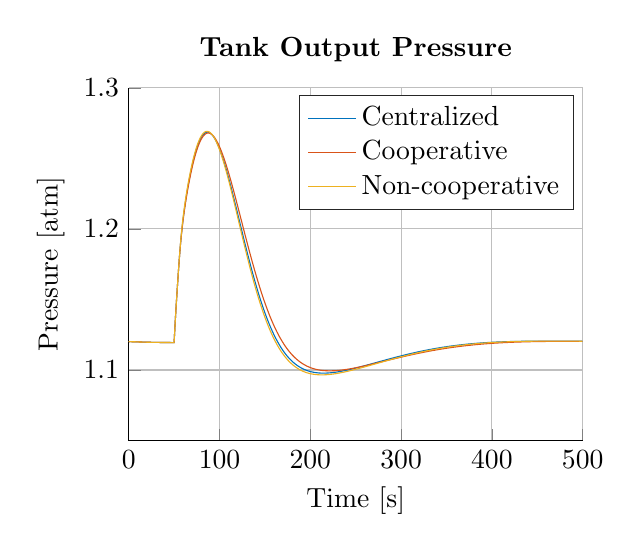
\begin{tikzpicture}

\begin{axis}[%
width=5.766cm,
height=4.479cm,
at={(0cm,0cm)},
scale only axis,
xmin=0,
xmax=500,
xlabel={Time [s]},
xmajorgrids,
ymin=1.05,
ymax=1.3,
ylabel={Pressure [atm]},
ymajorgrids,
axis background/.style={fill=white},
title style={font=\bfseries},
title={Tank Output Pressure},
axis x line*=bottom,
axis y line*=left,
legend style={legend cell align=left,align=left,draw=white!15!black}
]
\addplot [color=mycolor1,solid,forget plot]
  table[row sep=crcr]{%
0	1.12\\
0.5	1.12007\\
1	1.12008\\
1.5	1.12008\\
2	1.12008\\
2.5	1.12008\\
3	1.12008\\
3.5	1.12007\\
4	1.12007\\
4.5	1.12006\\
5	1.12005\\
5.5	1.12004\\
6	1.12003\\
6.5	1.12002\\
7	1.12001\\
7.5	1.12\\
8	1.11999\\
8.5	1.11997\\
9	1.11996\\
9.5	1.11995\\
10	1.11994\\
10.5	1.11992\\
11	1.11991\\
11.5	1.1199\\
12	1.11989\\
12.5	1.11987\\
13	1.11986\\
13.5	1.11985\\
14	1.11984\\
14.5	1.11983\\
15	1.11981\\
15.5	1.1198\\
16	1.11979\\
16.5	1.11978\\
17	1.11977\\
17.5	1.11976\\
18	1.11975\\
18.5	1.11974\\
19	1.11973\\
19.5	1.11973\\
20	1.11972\\
20.5	1.11971\\
21	1.1197\\
21.5	1.11969\\
22	1.11969\\
22.5	1.11968\\
23	1.11967\\
23.5	1.11966\\
24	1.11966\\
24.5	1.11965\\
25	1.11964\\
25.5	1.11964\\
26	1.11963\\
26.5	1.11962\\
27	1.11962\\
27.5	1.11961\\
28	1.11961\\
28.5	1.1196\\
29	1.1196\\
29.5	1.11959\\
30	1.11959\\
30.5	1.11958\\
31	1.11958\\
31.5	1.11957\\
32	1.11957\\
32.5	1.11956\\
33	1.11956\\
33.5	1.11955\\
34	1.11955\\
34.5	1.11954\\
35	1.11954\\
35.5	1.11954\\
36	1.11953\\
36.5	1.11953\\
37	1.11952\\
37.5	1.11952\\
38	1.11952\\
38.5	1.11951\\
39	1.11951\\
39.5	1.11951\\
40	1.1195\\
40.5	1.1195\\
41	1.1195\\
41.5	1.11949\\
42	1.11949\\
42.5	1.11949\\
43	1.11949\\
43.5	1.11948\\
44	1.11948\\
44.5	1.11948\\
45	1.11948\\
45.5	1.11947\\
46	1.11947\\
46.5	1.11947\\
47	1.11947\\
47.5	1.11946\\
48	1.11946\\
48.5	1.11946\\
49	1.11946\\
49.5	1.11946\\
50	1.11945\\
50.5	1.12569\\
51	1.13171\\
51.5	1.13735\\
52	1.14274\\
52.5	1.14794\\
53	1.153\\
53.5	1.15795\\
54	1.1628\\
54.5	1.16756\\
55	1.17229\\
55.5	1.17676\\
56	1.18105\\
56.5	1.18514\\
57	1.189\\
57.5	1.1926\\
58	1.19596\\
58.5	1.19912\\
59	1.2021\\
59.5	1.20491\\
60	1.20757\\
60.5	1.21011\\
61	1.21253\\
61.5	1.21486\\
62	1.21711\\
62.5	1.21928\\
63	1.22138\\
63.5	1.22342\\
64	1.22541\\
64.5	1.22733\\
65	1.22921\\
65.5	1.23103\\
66	1.2328\\
66.5	1.23452\\
67	1.2362\\
67.5	1.23784\\
68	1.23943\\
68.5	1.24099\\
69	1.2425\\
69.5	1.24397\\
70	1.2454\\
70.5	1.24679\\
71	1.24814\\
71.5	1.24944\\
72	1.2507\\
72.5	1.25192\\
73	1.2531\\
73.5	1.25424\\
74	1.25533\\
74.5	1.25637\\
75	1.25738\\
75.5	1.25834\\
76	1.25925\\
76.5	1.26012\\
77	1.26095\\
77.5	1.26174\\
78	1.26248\\
78.5	1.26317\\
79	1.26383\\
79.5	1.26444\\
80	1.26501\\
80.5	1.26553\\
81	1.26602\\
81.5	1.26646\\
82	1.26686\\
82.5	1.26721\\
83	1.26753\\
83.5	1.2678\\
84	1.26804\\
84.5	1.26823\\
85	1.26839\\
85.5	1.2685\\
86	1.26858\\
86.5	1.26861\\
87	1.26861\\
87.5	1.26857\\
88	1.26849\\
88.5	1.26838\\
89	1.26823\\
89.5	1.26804\\
90	1.26782\\
90.5	1.26756\\
91	1.26727\\
91.5	1.26695\\
92	1.26659\\
92.5	1.2662\\
93	1.26577\\
93.5	1.26532\\
94	1.26483\\
94.5	1.26431\\
95	1.26376\\
95.5	1.26318\\
96	1.26258\\
96.5	1.26194\\
97	1.26128\\
97.5	1.26059\\
98	1.25987\\
98.5	1.25913\\
99	1.25836\\
99.5	1.25757\\
100	1.25675\\
100.5	1.25591\\
101	1.25504\\
101.5	1.25415\\
102	1.25324\\
102.5	1.25231\\
103	1.25136\\
103.5	1.25039\\
104	1.2494\\
104.5	1.24839\\
105	1.24736\\
105.5	1.24631\\
106	1.24525\\
106.5	1.24417\\
107	1.24307\\
107.5	1.24196\\
108	1.24083\\
108.5	1.23969\\
109	1.23854\\
109.5	1.23737\\
110	1.23619\\
110.5	1.235\\
111	1.2338\\
111.5	1.23258\\
112	1.23136\\
112.5	1.23012\\
113	1.22888\\
113.5	1.22763\\
114	1.22637\\
114.5	1.2251\\
115	1.22382\\
115.5	1.22254\\
116	1.22126\\
116.5	1.21996\\
117	1.21866\\
117.5	1.21736\\
118	1.21606\\
118.5	1.21474\\
119	1.21343\\
119.5	1.21212\\
120	1.2108\\
120.5	1.20948\\
121	1.20816\\
121.5	1.20683\\
122	1.20551\\
122.5	1.20419\\
123	1.20287\\
123.5	1.20155\\
124	1.20023\\
124.5	1.19891\\
125	1.19759\\
125.5	1.19628\\
126	1.19497\\
126.5	1.19366\\
127	1.19235\\
127.5	1.19105\\
128	1.18976\\
128.5	1.18847\\
129	1.18718\\
129.5	1.1859\\
130	1.18462\\
130.5	1.18335\\
131	1.18208\\
131.5	1.18082\\
132	1.17957\\
132.5	1.17833\\
133	1.17709\\
133.5	1.17586\\
134	1.17464\\
134.5	1.17342\\
135	1.17221\\
135.5	1.17101\\
136	1.16982\\
136.5	1.16864\\
137	1.16747\\
137.5	1.1663\\
138	1.16515\\
138.5	1.164\\
139	1.16287\\
139.5	1.16174\\
140	1.16062\\
140.5	1.15952\\
141	1.15842\\
141.5	1.15734\\
142	1.15626\\
142.5	1.1552\\
143	1.15414\\
143.5	1.1531\\
144	1.15207\\
144.5	1.15104\\
145	1.15003\\
145.5	1.14903\\
146	1.14804\\
146.5	1.14707\\
147	1.1461\\
147.5	1.14514\\
148	1.1442\\
148.5	1.14327\\
149	1.14235\\
149.5	1.14144\\
150	1.14054\\
150.5	1.13965\\
151	1.13878\\
151.5	1.13792\\
152	1.13706\\
152.5	1.13622\\
153	1.13539\\
153.5	1.13458\\
154	1.13377\\
154.5	1.13297\\
155	1.13219\\
155.5	1.13142\\
156	1.13066\\
156.5	1.12991\\
157	1.12917\\
157.5	1.12844\\
158	1.12773\\
158.5	1.12702\\
159	1.12633\\
159.5	1.12565\\
160	1.12498\\
160.5	1.12432\\
161	1.12367\\
161.5	1.12303\\
162	1.1224\\
162.5	1.12178\\
163	1.12117\\
163.5	1.12058\\
164	1.11999\\
164.5	1.11941\\
165	1.11885\\
165.5	1.11829\\
166	1.11775\\
166.5	1.11721\\
167	1.11669\\
167.5	1.11617\\
168	1.11566\\
168.5	1.11517\\
169	1.11468\\
169.5	1.1142\\
170	1.11373\\
170.5	1.11327\\
171	1.11282\\
171.5	1.11238\\
172	1.11195\\
172.5	1.11153\\
173	1.11111\\
173.5	1.11071\\
174	1.11031\\
174.5	1.10992\\
175	1.10954\\
175.5	1.10917\\
176	1.1088\\
176.5	1.10844\\
177	1.1081\\
177.5	1.10775\\
178	1.10742\\
178.5	1.1071\\
179	1.10678\\
179.5	1.10647\\
180	1.10616\\
180.5	1.10587\\
181	1.10558\\
181.5	1.1053\\
182	1.10502\\
182.5	1.10475\\
183	1.10449\\
183.5	1.10423\\
184	1.10399\\
184.5	1.10374\\
185	1.10351\\
185.5	1.10328\\
186	1.10305\\
186.5	1.10284\\
187	1.10262\\
187.5	1.10242\\
188	1.10222\\
188.5	1.10202\\
189	1.10184\\
189.5	1.10165\\
190	1.10147\\
190.5	1.1013\\
191	1.10113\\
191.5	1.10097\\
192	1.10081\\
192.5	1.10066\\
193	1.10051\\
193.5	1.10037\\
194	1.10023\\
194.5	1.1001\\
195	1.09997\\
195.5	1.09985\\
196	1.09973\\
196.5	1.09961\\
197	1.0995\\
197.5	1.09939\\
198	1.09929\\
198.5	1.09919\\
199	1.0991\\
199.5	1.09901\\
200	1.09892\\
200.5	1.09884\\
201	1.09876\\
201.5	1.09868\\
202	1.09861\\
202.5	1.09854\\
203	1.09848\\
203.5	1.09841\\
204	1.09836\\
204.5	1.0983\\
205	1.09825\\
205.5	1.0982\\
206	1.09815\\
206.5	1.09811\\
207	1.09807\\
207.5	1.09803\\
208	1.098\\
208.5	1.09797\\
209	1.09794\\
209.5	1.09791\\
210	1.09789\\
210.5	1.09787\\
211	1.09785\\
211.5	1.09784\\
212	1.09782\\
212.5	1.09781\\
213	1.09781\\
213.5	1.0978\\
214	1.0978\\
214.5	1.0978\\
215	1.0978\\
215.5	1.0978\\
216	1.0978\\
216.5	1.09781\\
217	1.09782\\
217.5	1.09783\\
218	1.09785\\
218.5	1.09786\\
219	1.09788\\
219.5	1.0979\\
220	1.09792\\
220.5	1.09794\\
221	1.09796\\
221.5	1.09799\\
222	1.09802\\
222.5	1.09805\\
223	1.09808\\
223.5	1.09811\\
224	1.09814\\
224.5	1.09818\\
225	1.09822\\
225.5	1.09826\\
226	1.0983\\
226.5	1.09834\\
227	1.09838\\
227.5	1.09842\\
228	1.09847\\
228.5	1.09851\\
229	1.09856\\
229.5	1.09861\\
230	1.09866\\
230.5	1.09871\\
231	1.09876\\
231.5	1.09882\\
232	1.09887\\
232.5	1.09893\\
233	1.09899\\
233.5	1.09904\\
234	1.0991\\
234.5	1.09916\\
235	1.09922\\
235.5	1.09928\\
236	1.09935\\
236.5	1.09941\\
237	1.09947\\
237.5	1.09954\\
238	1.0996\\
238.5	1.09967\\
239	1.09974\\
239.5	1.09981\\
240	1.09988\\
240.5	1.09995\\
241	1.10002\\
241.5	1.10009\\
242	1.10016\\
242.5	1.10023\\
243	1.10031\\
243.5	1.10038\\
244	1.10045\\
244.5	1.10053\\
245	1.1006\\
245.5	1.10068\\
246	1.10076\\
246.5	1.10083\\
247	1.10091\\
247.5	1.10099\\
248	1.10107\\
248.5	1.10115\\
249	1.10123\\
249.5	1.10131\\
250	1.10139\\
};
\addplot [color=mycolor1,solid]
  table[row sep=crcr]{%
250	1.10139\\
250.5	1.10147\\
251	1.10155\\
251.5	1.10163\\
252	1.10172\\
252.5	1.1018\\
253	1.10188\\
253.5	1.10196\\
254	1.10205\\
254.5	1.10213\\
255	1.10222\\
255.5	1.1023\\
256	1.10239\\
256.5	1.10247\\
257	1.10256\\
257.5	1.10264\\
258	1.10273\\
258.5	1.10281\\
259	1.1029\\
259.5	1.10299\\
260	1.10307\\
260.5	1.10316\\
261	1.10325\\
261.5	1.10334\\
262	1.10342\\
262.5	1.10351\\
263	1.1036\\
263.5	1.10369\\
264	1.10378\\
264.5	1.10386\\
265	1.10395\\
265.5	1.10404\\
266	1.10413\\
266.5	1.10422\\
267	1.10431\\
267.5	1.1044\\
268	1.10448\\
268.5	1.10457\\
269	1.10466\\
269.5	1.10475\\
270	1.10484\\
270.5	1.10493\\
271	1.10502\\
271.5	1.10511\\
272	1.1052\\
272.5	1.10529\\
273	1.10538\\
273.5	1.10546\\
274	1.10555\\
274.5	1.10564\\
275	1.10573\\
275.5	1.10582\\
276	1.10591\\
276.5	1.106\\
277	1.10609\\
277.5	1.10618\\
278	1.10627\\
278.5	1.10635\\
279	1.10644\\
279.5	1.10653\\
280	1.10662\\
280.5	1.10671\\
281	1.1068\\
281.5	1.10688\\
282	1.10697\\
282.5	1.10706\\
283	1.10715\\
283.5	1.10724\\
284	1.10732\\
284.5	1.10741\\
285	1.1075\\
285.5	1.10759\\
286	1.10767\\
286.5	1.10776\\
287	1.10785\\
287.5	1.10793\\
288	1.10802\\
288.5	1.1081\\
289	1.10819\\
289.5	1.10828\\
290	1.10836\\
290.5	1.10845\\
291	1.10853\\
291.5	1.10862\\
292	1.1087\\
292.5	1.10879\\
293	1.10887\\
293.5	1.10896\\
294	1.10904\\
294.5	1.10912\\
295	1.10921\\
295.5	1.10929\\
296	1.10937\\
296.5	1.10946\\
297	1.10954\\
297.5	1.10962\\
298	1.1097\\
298.5	1.10979\\
299	1.10987\\
299.5	1.10995\\
300	1.11003\\
300.5	1.11011\\
301	1.11019\\
301.5	1.11027\\
302	1.11035\\
302.5	1.11043\\
303	1.11051\\
303.5	1.11059\\
304	1.11067\\
304.5	1.11075\\
305	1.11083\\
305.5	1.1109\\
306	1.11098\\
306.5	1.11106\\
307	1.11114\\
307.5	1.11121\\
308	1.11129\\
308.5	1.11137\\
309	1.11144\\
309.5	1.11152\\
310	1.11159\\
310.5	1.11167\\
311	1.11174\\
311.5	1.11182\\
312	1.11189\\
312.5	1.11197\\
313	1.11204\\
313.5	1.11211\\
314	1.11219\\
314.5	1.11226\\
315	1.11233\\
315.5	1.1124\\
316	1.11248\\
316.5	1.11255\\
317	1.11262\\
317.5	1.11269\\
318	1.11276\\
318.5	1.11283\\
319	1.1129\\
319.5	1.11297\\
320	1.11304\\
320.5	1.11311\\
321	1.11317\\
321.5	1.11324\\
322	1.11331\\
322.5	1.11338\\
323	1.11344\\
323.5	1.11351\\
324	1.11358\\
324.5	1.11364\\
325	1.11371\\
325.5	1.11377\\
326	1.11384\\
326.5	1.1139\\
327	1.11397\\
327.5	1.11403\\
328	1.11409\\
328.5	1.11416\\
329	1.11422\\
329.5	1.11428\\
330	1.11434\\
330.5	1.11441\\
331	1.11447\\
331.5	1.11453\\
332	1.11459\\
332.5	1.11465\\
333	1.11471\\
333.5	1.11477\\
334	1.11483\\
334.5	1.11489\\
335	1.11494\\
335.5	1.115\\
336	1.11506\\
336.5	1.11512\\
337	1.11517\\
337.5	1.11523\\
338	1.11529\\
338.5	1.11534\\
339	1.1154\\
339.5	1.11545\\
340	1.11551\\
340.5	1.11556\\
341	1.11562\\
341.5	1.11567\\
342	1.11572\\
342.5	1.11578\\
343	1.11583\\
343.5	1.11588\\
344	1.11593\\
344.5	1.11599\\
345	1.11604\\
345.5	1.11609\\
346	1.11614\\
346.5	1.11619\\
347	1.11624\\
347.5	1.11629\\
348	1.11634\\
348.5	1.11639\\
349	1.11643\\
349.5	1.11648\\
350	1.11653\\
350.5	1.11658\\
351	1.11662\\
351.5	1.11667\\
352	1.11672\\
352.5	1.11676\\
353	1.11681\\
353.5	1.11685\\
354	1.1169\\
354.5	1.11694\\
355	1.11699\\
355.5	1.11703\\
356	1.11707\\
356.5	1.11712\\
357	1.11716\\
357.5	1.1172\\
358	1.11724\\
358.5	1.11729\\
359	1.11733\\
359.5	1.11737\\
360	1.11741\\
360.5	1.11745\\
361	1.11749\\
361.5	1.11753\\
362	1.11757\\
362.5	1.11761\\
363	1.11765\\
363.5	1.11768\\
364	1.11772\\
364.5	1.11776\\
365	1.1178\\
365.5	1.11783\\
366	1.11787\\
366.5	1.11791\\
367	1.11794\\
367.5	1.11798\\
368	1.11801\\
368.5	1.11805\\
369	1.11808\\
369.5	1.11812\\
370	1.11815\\
370.5	1.11819\\
371	1.11822\\
371.5	1.11825\\
372	1.11829\\
372.5	1.11832\\
373	1.11835\\
373.5	1.11838\\
374	1.11841\\
374.5	1.11844\\
375	1.11848\\
375.5	1.11851\\
376	1.11854\\
376.5	1.11857\\
377	1.1186\\
377.5	1.11863\\
378	1.11865\\
378.5	1.11868\\
379	1.11871\\
379.5	1.11874\\
380	1.11877\\
380.5	1.1188\\
381	1.11882\\
381.5	1.11885\\
382	1.11888\\
382.5	1.1189\\
383	1.11893\\
383.5	1.11895\\
384	1.11898\\
384.5	1.11901\\
385	1.11903\\
385.5	1.11906\\
386	1.11908\\
386.5	1.1191\\
387	1.11913\\
387.5	1.11915\\
388	1.11917\\
388.5	1.1192\\
389	1.11922\\
389.5	1.11924\\
390	1.11927\\
390.5	1.11929\\
391	1.11931\\
391.5	1.11933\\
392	1.11935\\
392.5	1.11937\\
393	1.11939\\
393.5	1.11941\\
394	1.11943\\
394.5	1.11945\\
395	1.11947\\
395.5	1.11949\\
396	1.11951\\
396.5	1.11953\\
397	1.11955\\
397.5	1.11957\\
398	1.11959\\
398.5	1.11961\\
399	1.11962\\
399.5	1.11964\\
400	1.11966\\
400.5	1.11968\\
401	1.11969\\
401.5	1.11971\\
402	1.11973\\
402.5	1.11974\\
403	1.11976\\
403.5	1.11977\\
404	1.11979\\
404.5	1.1198\\
405	1.11982\\
405.5	1.11983\\
406	1.11985\\
406.5	1.11986\\
407	1.11988\\
407.5	1.11989\\
408	1.11991\\
408.5	1.11992\\
409	1.11993\\
409.5	1.11995\\
410	1.11996\\
410.5	1.11997\\
411	1.11998\\
411.5	1.12\\
412	1.12001\\
412.5	1.12002\\
413	1.12003\\
413.5	1.12004\\
414	1.12006\\
414.5	1.12007\\
415	1.12008\\
415.5	1.12009\\
416	1.1201\\
416.5	1.12011\\
417	1.12012\\
417.5	1.12013\\
418	1.12014\\
418.5	1.12015\\
419	1.12016\\
419.5	1.12017\\
420	1.12018\\
420.5	1.12019\\
421	1.1202\\
421.5	1.12021\\
422	1.12021\\
422.5	1.12022\\
423	1.12023\\
423.5	1.12024\\
424	1.12025\\
424.5	1.12025\\
425	1.12026\\
425.5	1.12027\\
426	1.12028\\
426.5	1.12028\\
427	1.12029\\
427.5	1.1203\\
428	1.12031\\
428.5	1.12031\\
429	1.12032\\
429.5	1.12032\\
430	1.12033\\
430.5	1.12034\\
431	1.12034\\
431.5	1.12035\\
432	1.12035\\
432.5	1.12036\\
433	1.12037\\
433.5	1.12037\\
434	1.12038\\
434.5	1.12038\\
435	1.12039\\
435.5	1.12039\\
436	1.1204\\
436.5	1.1204\\
437	1.1204\\
437.5	1.12041\\
438	1.12041\\
438.5	1.12042\\
439	1.12042\\
439.5	1.12042\\
440	1.12043\\
440.5	1.12043\\
441	1.12044\\
441.5	1.12044\\
442	1.12044\\
442.5	1.12045\\
443	1.12045\\
443.5	1.12045\\
444	1.12045\\
444.5	1.12046\\
445	1.12046\\
445.5	1.12046\\
446	1.12046\\
446.5	1.12047\\
447	1.12047\\
447.5	1.12047\\
448	1.12047\\
448.5	1.12048\\
449	1.12048\\
449.5	1.12048\\
450	1.12048\\
450.5	1.12048\\
451	1.12048\\
451.5	1.12049\\
452	1.12049\\
452.5	1.12049\\
453	1.12049\\
453.5	1.12049\\
454	1.12049\\
454.5	1.12049\\
455	1.12049\\
455.5	1.12049\\
456	1.1205\\
456.5	1.1205\\
457	1.1205\\
457.5	1.1205\\
458	1.1205\\
458.5	1.1205\\
459	1.1205\\
459.5	1.1205\\
460	1.1205\\
460.5	1.1205\\
461	1.1205\\
461.5	1.1205\\
462	1.1205\\
462.5	1.1205\\
463	1.1205\\
463.5	1.1205\\
464	1.1205\\
464.5	1.1205\\
465	1.1205\\
465.5	1.1205\\
466	1.1205\\
466.5	1.1205\\
467	1.1205\\
467.5	1.1205\\
468	1.12049\\
468.5	1.12049\\
469	1.12049\\
469.5	1.12049\\
470	1.12049\\
470.5	1.12049\\
471	1.12049\\
471.5	1.12049\\
472	1.12049\\
472.5	1.12049\\
473	1.12049\\
473.5	1.12048\\
474	1.12048\\
474.5	1.12048\\
475	1.12048\\
475.5	1.12048\\
476	1.12048\\
476.5	1.12048\\
477	1.12047\\
477.5	1.12047\\
478	1.12047\\
478.5	1.12047\\
479	1.12047\\
479.5	1.12047\\
480	1.12046\\
480.5	1.12046\\
481	1.12046\\
481.5	1.12046\\
482	1.12046\\
482.5	1.12046\\
483	1.12045\\
483.5	1.12045\\
484	1.12045\\
484.5	1.12045\\
485	1.12045\\
485.5	1.12044\\
486	1.12044\\
486.5	1.12044\\
487	1.12044\\
487.5	1.12044\\
488	1.12043\\
488.5	1.12043\\
489	1.12043\\
489.5	1.12043\\
490	1.12043\\
490.5	1.12042\\
491	1.12042\\
491.5	1.12042\\
492	1.12042\\
492.5	1.12042\\
493	1.12041\\
493.5	1.12041\\
494	1.12041\\
494.5	1.12041\\
495	1.1204\\
495.5	1.1204\\
496	1.1204\\
496.5	1.1204\\
497	1.12039\\
497.5	1.12039\\
498	1.12039\\
498.5	1.12039\\
499	1.12038\\
499.5	1.12038\\
};
\addlegendentry{Centralized};

\addplot [color=mycolor2,solid,forget plot]
  table[row sep=crcr]{%
0	1.12\\
0.5	1.12007\\
1	1.12008\\
1.5	1.12008\\
2	1.12008\\
2.5	1.12008\\
3	1.12008\\
3.5	1.12007\\
4	1.12006\\
4.5	1.12006\\
5	1.12005\\
5.5	1.12004\\
6	1.12003\\
6.5	1.12002\\
7	1.12001\\
7.5	1.11999\\
8	1.11998\\
8.5	1.11997\\
9	1.11996\\
9.5	1.11994\\
10	1.11993\\
10.5	1.11992\\
11	1.1199\\
11.5	1.11989\\
12	1.11988\\
12.5	1.11987\\
13	1.11985\\
13.5	1.11984\\
14	1.11983\\
14.5	1.11982\\
15	1.11981\\
15.5	1.1198\\
16	1.11979\\
16.5	1.11978\\
17	1.11977\\
17.5	1.11976\\
18	1.11975\\
18.5	1.11974\\
19	1.11973\\
19.5	1.11972\\
20	1.11971\\
20.5	1.1197\\
21	1.11969\\
21.5	1.11969\\
22	1.11968\\
22.5	1.11967\\
23	1.11966\\
23.5	1.11966\\
24	1.11965\\
24.5	1.11964\\
25	1.11964\\
25.5	1.11963\\
26	1.11962\\
26.5	1.11962\\
27	1.11961\\
27.5	1.11961\\
28	1.1196\\
28.5	1.11959\\
29	1.11959\\
29.5	1.11958\\
30	1.11958\\
30.5	1.11957\\
31	1.11957\\
31.5	1.11956\\
32	1.11956\\
32.5	1.11955\\
33	1.11955\\
33.5	1.11955\\
34	1.11954\\
34.5	1.11954\\
35	1.11953\\
35.5	1.11953\\
36	1.11952\\
36.5	1.11952\\
37	1.11952\\
37.5	1.11951\\
38	1.11951\\
38.5	1.11951\\
39	1.1195\\
39.5	1.1195\\
40	1.1195\\
40.5	1.11949\\
41	1.11949\\
41.5	1.11949\\
42	1.11948\\
42.5	1.11948\\
43	1.11948\\
43.5	1.11948\\
44	1.11947\\
44.5	1.11947\\
45	1.11947\\
45.5	1.11947\\
46	1.11946\\
46.5	1.11946\\
47	1.11946\\
47.5	1.11946\\
48	1.11945\\
48.5	1.11945\\
49	1.11945\\
49.5	1.11945\\
50	1.11944\\
50.5	1.12568\\
51	1.1317\\
51.5	1.13734\\
52	1.14274\\
52.5	1.14796\\
53	1.15303\\
53.5	1.15798\\
54	1.16283\\
54.5	1.16759\\
55	1.17228\\
55.5	1.1767\\
56	1.18091\\
56.5	1.18494\\
57	1.1887\\
57.5	1.19219\\
58	1.19546\\
58.5	1.19852\\
59	1.20141\\
59.5	1.20413\\
60	1.20672\\
60.5	1.20919\\
61	1.21156\\
61.5	1.21385\\
62	1.21606\\
62.5	1.2182\\
63	1.22027\\
63.5	1.22229\\
64	1.22426\\
64.5	1.22616\\
65	1.22801\\
65.5	1.2298\\
66	1.23154\\
66.5	1.23324\\
67	1.2349\\
67.5	1.23651\\
68	1.23808\\
68.5	1.23961\\
69	1.24111\\
69.5	1.24256\\
70	1.24398\\
70.5	1.24535\\
71	1.24669\\
71.5	1.24798\\
72	1.24924\\
72.5	1.25045\\
73	1.25162\\
73.5	1.25275\\
74	1.25385\\
74.5	1.25489\\
75	1.2559\\
75.5	1.25687\\
76	1.2578\\
76.5	1.25868\\
77	1.25952\\
77.5	1.26033\\
78	1.26109\\
78.5	1.26181\\
79	1.26248\\
79.5	1.26312\\
80	1.26372\\
80.5	1.26428\\
81	1.26479\\
81.5	1.26527\\
82	1.26571\\
82.5	1.26611\\
83	1.26647\\
83.5	1.26679\\
84	1.26707\\
84.5	1.26731\\
85	1.26752\\
85.5	1.26769\\
86	1.26782\\
86.5	1.26792\\
87	1.26798\\
87.5	1.268\\
88	1.26799\\
88.5	1.26794\\
89	1.26786\\
89.5	1.26775\\
90	1.2676\\
90.5	1.26741\\
91	1.2672\\
91.5	1.26695\\
92	1.26667\\
92.5	1.26636\\
93	1.26602\\
93.5	1.26565\\
94	1.26525\\
94.5	1.26482\\
95	1.26436\\
95.5	1.26387\\
96	1.26335\\
96.5	1.26281\\
97	1.26224\\
97.5	1.26164\\
98	1.26102\\
98.5	1.26037\\
99	1.2597\\
99.5	1.259\\
100	1.25828\\
100.5	1.25754\\
101	1.25678\\
101.5	1.25599\\
102	1.25518\\
102.5	1.25435\\
103	1.2535\\
103.5	1.25263\\
104	1.25174\\
104.5	1.25083\\
105	1.24991\\
105.5	1.24896\\
106	1.248\\
106.5	1.24702\\
107	1.24603\\
107.5	1.24502\\
108	1.24399\\
108.5	1.24295\\
109	1.2419\\
109.5	1.24083\\
110	1.23975\\
110.5	1.23866\\
111	1.23755\\
111.5	1.23644\\
112	1.23531\\
112.5	1.23417\\
113	1.23302\\
113.5	1.23187\\
114	1.2307\\
114.5	1.22953\\
115	1.22834\\
115.5	1.22715\\
116	1.22595\\
116.5	1.22475\\
117	1.22354\\
117.5	1.22232\\
118	1.2211\\
118.5	1.21987\\
119	1.21864\\
119.5	1.21741\\
120	1.21617\\
120.5	1.21493\\
121	1.21368\\
121.5	1.21244\\
122	1.21119\\
122.5	1.20994\\
123	1.20868\\
123.5	1.20743\\
124	1.20618\\
124.5	1.20493\\
125	1.20367\\
125.5	1.20242\\
126	1.20117\\
126.5	1.19992\\
127	1.19867\\
127.5	1.19743\\
128	1.19618\\
128.5	1.19494\\
129	1.19371\\
129.5	1.19247\\
130	1.19124\\
130.5	1.19001\\
131	1.18879\\
131.5	1.18757\\
132	1.18636\\
132.5	1.18515\\
133	1.18395\\
133.5	1.18275\\
134	1.18156\\
134.5	1.18037\\
135	1.17919\\
135.5	1.17802\\
136	1.17685\\
136.5	1.17569\\
137	1.17454\\
137.5	1.1734\\
138	1.17226\\
138.5	1.17113\\
139	1.17001\\
139.5	1.16889\\
140	1.16779\\
140.5	1.16669\\
141	1.1656\\
141.5	1.16452\\
142	1.16345\\
142.5	1.16238\\
143	1.16133\\
143.5	1.16028\\
144	1.15925\\
144.5	1.15822\\
145	1.1572\\
145.5	1.1562\\
146	1.1552\\
146.5	1.15421\\
147	1.15323\\
147.5	1.15226\\
148	1.15131\\
148.5	1.15036\\
149	1.14942\\
149.5	1.14849\\
150	1.14757\\
150.5	1.14667\\
151	1.14577\\
151.5	1.14488\\
152	1.14401\\
152.5	1.14314\\
153	1.14228\\
153.5	1.14144\\
154	1.1406\\
154.5	1.13978\\
155	1.13897\\
155.5	1.13816\\
156	1.13737\\
156.5	1.13659\\
157	1.13581\\
157.5	1.13505\\
158	1.1343\\
158.5	1.13356\\
159	1.13283\\
159.5	1.13211\\
160	1.1314\\
160.5	1.1307\\
161	1.13001\\
161.5	1.12933\\
162	1.12866\\
162.5	1.128\\
163	1.12735\\
163.5	1.12671\\
164	1.12608\\
164.5	1.12546\\
165	1.12485\\
165.5	1.12425\\
166	1.12366\\
166.5	1.12308\\
167	1.1225\\
167.5	1.12194\\
168	1.12139\\
168.5	1.12084\\
169	1.12031\\
169.5	1.11979\\
170	1.11927\\
170.5	1.11876\\
171	1.11826\\
171.5	1.11778\\
172	1.11729\\
172.5	1.11682\\
173	1.11636\\
173.5	1.11591\\
174	1.11546\\
174.5	1.11502\\
175	1.11459\\
175.5	1.11417\\
176	1.11376\\
176.5	1.11335\\
177	1.11295\\
177.5	1.11257\\
178	1.11218\\
178.5	1.11181\\
179	1.11144\\
179.5	1.11108\\
180	1.11073\\
180.5	1.11039\\
181	1.11005\\
181.5	1.10972\\
182	1.1094\\
182.5	1.10908\\
183	1.10877\\
183.5	1.10847\\
184	1.10817\\
184.5	1.10789\\
185	1.1076\\
185.5	1.10733\\
186	1.10706\\
186.5	1.10679\\
187	1.10654\\
187.5	1.10628\\
188	1.10604\\
188.5	1.1058\\
189	1.10557\\
189.5	1.10534\\
190	1.10512\\
190.5	1.1049\\
191	1.10469\\
191.5	1.10448\\
192	1.10428\\
192.5	1.10409\\
193	1.1039\\
193.5	1.10371\\
194	1.10353\\
194.5	1.10336\\
195	1.10319\\
195.5	1.10302\\
196	1.10286\\
196.5	1.1027\\
197	1.10255\\
197.5	1.10241\\
198	1.10226\\
198.5	1.10213\\
199	1.10199\\
199.5	1.10186\\
200	1.10174\\
200.5	1.10161\\
201	1.1015\\
201.5	1.10138\\
202	1.10127\\
202.5	1.10117\\
203	1.10107\\
203.5	1.10097\\
204	1.10087\\
204.5	1.10078\\
205	1.10069\\
205.5	1.10061\\
206	1.10053\\
206.5	1.10045\\
207	1.10038\\
207.5	1.10031\\
208	1.10024\\
208.5	1.10017\\
209	1.10011\\
209.5	1.10005\\
210	1.1\\
210.5	1.09994\\
211	1.09989\\
211.5	1.09985\\
212	1.0998\\
212.5	1.09976\\
213	1.09972\\
213.5	1.09968\\
214	1.09965\\
214.5	1.09962\\
215	1.09959\\
215.5	1.09956\\
216	1.09954\\
216.5	1.09952\\
217	1.0995\\
217.5	1.09948\\
218	1.09946\\
218.5	1.09945\\
219	1.09944\\
219.5	1.09943\\
220	1.09942\\
220.5	1.09942\\
221	1.09941\\
221.5	1.09941\\
222	1.09941\\
222.5	1.09942\\
223	1.09942\\
223.5	1.09943\\
224	1.09944\\
224.5	1.09945\\
225	1.09946\\
225.5	1.09947\\
226	1.09949\\
226.5	1.0995\\
227	1.09952\\
227.5	1.09954\\
228	1.09956\\
228.5	1.09958\\
229	1.09961\\
229.5	1.09963\\
230	1.09966\\
230.5	1.09969\\
231	1.09972\\
231.5	1.09975\\
232	1.09978\\
232.5	1.09981\\
233	1.09985\\
233.5	1.09988\\
234	1.09992\\
234.5	1.09996\\
235	1.1\\
235.5	1.10004\\
236	1.10008\\
236.5	1.10012\\
237	1.10017\\
237.5	1.10021\\
238	1.10026\\
238.5	1.1003\\
239	1.10035\\
239.5	1.1004\\
240	1.10045\\
240.5	1.1005\\
241	1.10055\\
241.5	1.1006\\
242	1.10065\\
242.5	1.10071\\
243	1.10076\\
243.5	1.10082\\
244	1.10087\\
244.5	1.10093\\
245	1.10099\\
245.5	1.10104\\
246	1.1011\\
246.5	1.10116\\
247	1.10122\\
247.5	1.10128\\
248	1.10134\\
248.5	1.10141\\
249	1.10147\\
249.5	1.10153\\
250	1.1016\\
};
\addplot [color=mycolor2,solid]
  table[row sep=crcr]{%
250	1.1016\\
250.5	1.10166\\
251	1.10173\\
251.5	1.10179\\
252	1.10186\\
252.5	1.10192\\
253	1.10199\\
253.5	1.10206\\
254	1.10213\\
254.5	1.10219\\
255	1.10226\\
255.5	1.10233\\
256	1.1024\\
256.5	1.10247\\
257	1.10254\\
257.5	1.10261\\
258	1.10268\\
258.5	1.10276\\
259	1.10283\\
259.5	1.1029\\
260	1.10297\\
260.5	1.10304\\
261	1.10312\\
261.5	1.10319\\
262	1.10326\\
262.5	1.10334\\
263	1.10341\\
263.5	1.10349\\
264	1.10356\\
264.5	1.10364\\
265	1.10371\\
265.5	1.10379\\
266	1.10386\\
266.5	1.10394\\
267	1.10402\\
267.5	1.10409\\
268	1.10417\\
268.5	1.10425\\
269	1.10432\\
269.5	1.1044\\
270	1.10448\\
270.5	1.10455\\
271	1.10463\\
271.5	1.10471\\
272	1.10479\\
272.5	1.10486\\
273	1.10494\\
273.5	1.10502\\
274	1.1051\\
274.5	1.10517\\
275	1.10525\\
275.5	1.10533\\
276	1.10541\\
276.5	1.10549\\
277	1.10557\\
277.5	1.10564\\
278	1.10572\\
278.5	1.1058\\
279	1.10588\\
279.5	1.10596\\
280	1.10604\\
280.5	1.10611\\
281	1.10619\\
281.5	1.10627\\
282	1.10635\\
282.5	1.10643\\
283	1.10651\\
283.5	1.10659\\
284	1.10666\\
284.5	1.10674\\
285	1.10682\\
285.5	1.1069\\
286	1.10698\\
286.5	1.10705\\
287	1.10713\\
287.5	1.10721\\
288	1.10729\\
288.5	1.10737\\
289	1.10744\\
289.5	1.10752\\
290	1.1076\\
290.5	1.10768\\
291	1.10775\\
291.5	1.10783\\
292	1.10791\\
292.5	1.10799\\
293	1.10806\\
293.5	1.10814\\
294	1.10822\\
294.5	1.10829\\
295	1.10837\\
295.5	1.10845\\
296	1.10852\\
296.5	1.1086\\
297	1.10867\\
297.5	1.10875\\
298	1.10883\\
298.5	1.1089\\
299	1.10898\\
299.5	1.10905\\
300	1.10913\\
300.5	1.1092\\
301	1.10928\\
301.5	1.10935\\
302	1.10942\\
302.5	1.1095\\
303	1.10957\\
303.5	1.10965\\
304	1.10972\\
304.5	1.10979\\
305	1.10987\\
305.5	1.10994\\
306	1.11001\\
306.5	1.11008\\
307	1.11016\\
307.5	1.11023\\
308	1.1103\\
308.5	1.11037\\
309	1.11044\\
309.5	1.11051\\
310	1.11059\\
310.5	1.11066\\
311	1.11073\\
311.5	1.1108\\
312	1.11087\\
312.5	1.11094\\
313	1.11101\\
313.5	1.11108\\
314	1.11115\\
314.5	1.11122\\
315	1.11128\\
315.5	1.11135\\
316	1.11142\\
316.5	1.11149\\
317	1.11156\\
317.5	1.11162\\
318	1.11169\\
318.5	1.11176\\
319	1.11183\\
319.5	1.11189\\
320	1.11196\\
320.5	1.11202\\
321	1.11209\\
321.5	1.11216\\
322	1.11222\\
322.5	1.11229\\
323	1.11235\\
323.5	1.11241\\
324	1.11248\\
324.5	1.11254\\
325	1.11261\\
325.5	1.11267\\
326	1.11273\\
326.5	1.1128\\
327	1.11286\\
327.5	1.11292\\
328	1.11298\\
328.5	1.11304\\
329	1.11311\\
329.5	1.11317\\
330	1.11323\\
330.5	1.11329\\
331	1.11335\\
331.5	1.11341\\
332	1.11347\\
332.5	1.11353\\
333	1.11359\\
333.5	1.11365\\
334	1.1137\\
334.5	1.11376\\
335	1.11382\\
335.5	1.11388\\
336	1.11393\\
336.5	1.11399\\
337	1.11405\\
337.5	1.11411\\
338	1.11416\\
338.5	1.11422\\
339	1.11427\\
339.5	1.11433\\
340	1.11438\\
340.5	1.11444\\
341	1.11449\\
341.5	1.11455\\
342	1.1146\\
342.5	1.11465\\
343	1.11471\\
343.5	1.11476\\
344	1.11481\\
344.5	1.11487\\
345	1.11492\\
345.5	1.11497\\
346	1.11502\\
346.5	1.11507\\
347	1.11512\\
347.5	1.11517\\
348	1.11522\\
348.5	1.11527\\
349	1.11532\\
349.5	1.11537\\
350	1.11542\\
350.5	1.11547\\
351	1.11552\\
351.5	1.11557\\
352	1.11562\\
352.5	1.11566\\
353	1.11571\\
353.5	1.11576\\
354	1.1158\\
354.5	1.11585\\
355	1.1159\\
355.5	1.11594\\
356	1.11599\\
356.5	1.11603\\
357	1.11608\\
357.5	1.11612\\
358	1.11617\\
358.5	1.11621\\
359	1.11626\\
359.5	1.1163\\
360	1.11634\\
360.5	1.11638\\
361	1.11643\\
361.5	1.11647\\
362	1.11651\\
362.5	1.11655\\
363	1.11659\\
363.5	1.11664\\
364	1.11668\\
364.5	1.11672\\
365	1.11676\\
365.5	1.1168\\
366	1.11684\\
366.5	1.11688\\
367	1.11692\\
367.5	1.11695\\
368	1.11699\\
368.5	1.11703\\
369	1.11707\\
369.5	1.11711\\
370	1.11714\\
370.5	1.11718\\
371	1.11722\\
371.5	1.11725\\
372	1.11729\\
372.5	1.11733\\
373	1.11736\\
373.5	1.1174\\
374	1.11743\\
374.5	1.11747\\
375	1.1175\\
375.5	1.11754\\
376	1.11757\\
376.5	1.1176\\
377	1.11764\\
377.5	1.11767\\
378	1.1177\\
378.5	1.11774\\
379	1.11777\\
379.5	1.1178\\
380	1.11783\\
380.5	1.11786\\
381	1.1179\\
381.5	1.11793\\
382	1.11796\\
382.5	1.11799\\
383	1.11802\\
383.5	1.11805\\
384	1.11808\\
384.5	1.11811\\
385	1.11814\\
385.5	1.11817\\
386	1.1182\\
386.5	1.11822\\
387	1.11825\\
387.5	1.11828\\
388	1.11831\\
388.5	1.11833\\
389	1.11836\\
389.5	1.11839\\
390	1.11842\\
390.5	1.11844\\
391	1.11847\\
391.5	1.11849\\
392	1.11852\\
392.5	1.11855\\
393	1.11857\\
393.5	1.1186\\
394	1.11862\\
394.5	1.11865\\
395	1.11867\\
395.5	1.11869\\
396	1.11872\\
396.5	1.11874\\
397	1.11876\\
397.5	1.11879\\
398	1.11881\\
398.5	1.11883\\
399	1.11886\\
399.5	1.11888\\
400	1.1189\\
400.5	1.11892\\
401	1.11894\\
401.5	1.11896\\
402	1.11899\\
402.5	1.11901\\
403	1.11903\\
403.5	1.11905\\
404	1.11907\\
404.5	1.11909\\
405	1.11911\\
405.5	1.11913\\
406	1.11915\\
406.5	1.11917\\
407	1.11918\\
407.5	1.1192\\
408	1.11922\\
408.5	1.11924\\
409	1.11926\\
409.5	1.11928\\
410	1.11929\\
410.5	1.11931\\
411	1.11933\\
411.5	1.11935\\
412	1.11936\\
412.5	1.11938\\
413	1.1194\\
413.5	1.11941\\
414	1.11943\\
414.5	1.11945\\
415	1.11946\\
415.5	1.11948\\
416	1.11949\\
416.5	1.11951\\
417	1.11952\\
417.5	1.11954\\
418	1.11955\\
418.5	1.11957\\
419	1.11958\\
419.5	1.11959\\
420	1.11961\\
420.5	1.11962\\
421	1.11964\\
421.5	1.11965\\
422	1.11966\\
422.5	1.11968\\
423	1.11969\\
423.5	1.1197\\
424	1.11971\\
424.5	1.11973\\
425	1.11974\\
425.5	1.11975\\
426	1.11976\\
426.5	1.11977\\
427	1.11979\\
427.5	1.1198\\
428	1.11981\\
428.5	1.11982\\
429	1.11983\\
429.5	1.11984\\
430	1.11985\\
430.5	1.11986\\
431	1.11987\\
431.5	1.11988\\
432	1.11989\\
432.5	1.1199\\
433	1.11991\\
433.5	1.11992\\
434	1.11993\\
434.5	1.11994\\
435	1.11995\\
435.5	1.11996\\
436	1.11997\\
436.5	1.11998\\
437	1.11999\\
437.5	1.12\\
438	1.12\\
438.5	1.12001\\
439	1.12002\\
439.5	1.12003\\
440	1.12004\\
440.5	1.12004\\
441	1.12005\\
441.5	1.12006\\
442	1.12007\\
442.5	1.12007\\
443	1.12008\\
443.5	1.12009\\
444	1.1201\\
444.5	1.1201\\
445	1.12011\\
445.5	1.12012\\
446	1.12012\\
446.5	1.12013\\
447	1.12013\\
447.5	1.12014\\
448	1.12015\\
448.5	1.12015\\
449	1.12016\\
449.5	1.12016\\
450	1.12017\\
450.5	1.12017\\
451	1.12018\\
451.5	1.12019\\
452	1.12019\\
452.5	1.1202\\
453	1.1202\\
453.5	1.12021\\
454	1.12021\\
454.5	1.12021\\
455	1.12022\\
455.5	1.12022\\
456	1.12023\\
456.5	1.12023\\
457	1.12024\\
457.5	1.12024\\
458	1.12024\\
458.5	1.12025\\
459	1.12025\\
459.5	1.12026\\
460	1.12026\\
460.5	1.12026\\
461	1.12027\\
461.5	1.12027\\
462	1.12027\\
462.5	1.12028\\
463	1.12028\\
463.5	1.12028\\
464	1.12029\\
464.5	1.12029\\
465	1.12029\\
465.5	1.12029\\
466	1.1203\\
466.5	1.1203\\
467	1.1203\\
467.5	1.1203\\
468	1.12031\\
468.5	1.12031\\
469	1.12031\\
469.5	1.12031\\
470	1.12032\\
470.5	1.12032\\
471	1.12032\\
471.5	1.12032\\
472	1.12032\\
472.5	1.12033\\
473	1.12033\\
473.5	1.12033\\
474	1.12033\\
474.5	1.12033\\
475	1.12033\\
475.5	1.12033\\
476	1.12034\\
476.5	1.12034\\
477	1.12034\\
477.5	1.12034\\
478	1.12034\\
478.5	1.12034\\
479	1.12034\\
479.5	1.12034\\
480	1.12034\\
480.5	1.12035\\
481	1.12035\\
481.5	1.12035\\
482	1.12035\\
482.5	1.12035\\
483	1.12035\\
483.5	1.12035\\
484	1.12035\\
484.5	1.12035\\
485	1.12035\\
485.5	1.12035\\
486	1.12035\\
486.5	1.12035\\
487	1.12035\\
487.5	1.12035\\
488	1.12035\\
488.5	1.12035\\
489	1.12035\\
489.5	1.12035\\
490	1.12035\\
490.5	1.12035\\
491	1.12035\\
491.5	1.12035\\
492	1.12035\\
492.5	1.12035\\
493	1.12035\\
493.5	1.12035\\
494	1.12035\\
494.5	1.12035\\
495	1.12035\\
495.5	1.12035\\
496	1.12035\\
496.5	1.12035\\
497	1.12035\\
497.5	1.12035\\
498	1.12035\\
498.5	1.12035\\
499	1.12035\\
499.5	1.12034\\
};
\addlegendentry{Cooperative};

\addplot [color=mycolor3,solid,forget plot]
  table[row sep=crcr]{%
0	1.12\\
0.5	1.12007\\
1	1.12008\\
1.5	1.12008\\
2	1.12008\\
2.5	1.12008\\
3	1.12008\\
3.5	1.12007\\
4	1.12007\\
4.5	1.12006\\
5	1.12005\\
5.5	1.12004\\
6	1.12003\\
6.5	1.12002\\
7	1.12001\\
7.5	1.12\\
8	1.11998\\
8.5	1.11997\\
9	1.11996\\
9.5	1.11995\\
10	1.11993\\
10.5	1.11992\\
11	1.11991\\
11.5	1.11989\\
12	1.11988\\
12.5	1.11987\\
13	1.11986\\
13.5	1.11984\\
14	1.11983\\
14.5	1.11982\\
15	1.11981\\
15.5	1.1198\\
16	1.11979\\
16.5	1.11978\\
17	1.11977\\
17.5	1.11976\\
18	1.11975\\
18.5	1.11974\\
19	1.11973\\
19.5	1.11972\\
20	1.11971\\
20.5	1.1197\\
21	1.1197\\
21.5	1.11969\\
22	1.11968\\
22.5	1.11967\\
23	1.11967\\
23.5	1.11966\\
24	1.11965\\
24.5	1.11964\\
25	1.11964\\
25.5	1.11963\\
26	1.11963\\
26.5	1.11962\\
27	1.11961\\
27.5	1.11961\\
28	1.1196\\
28.5	1.1196\\
29	1.11959\\
29.5	1.11959\\
30	1.11958\\
30.5	1.11958\\
31	1.11957\\
31.5	1.11957\\
32	1.11956\\
32.5	1.11956\\
33	1.11955\\
33.5	1.11955\\
34	1.11954\\
34.5	1.11954\\
35	1.11954\\
35.5	1.11953\\
36	1.11953\\
36.5	1.11952\\
37	1.11952\\
37.5	1.11952\\
38	1.11951\\
38.5	1.11951\\
39	1.11951\\
39.5	1.1195\\
40	1.1195\\
40.5	1.1195\\
41	1.11949\\
41.5	1.11949\\
42	1.11949\\
42.5	1.11948\\
43	1.11948\\
43.5	1.11948\\
44	1.11948\\
44.5	1.11947\\
45	1.11947\\
45.5	1.11947\\
46	1.11947\\
46.5	1.11946\\
47	1.11946\\
47.5	1.11946\\
48	1.11946\\
48.5	1.11946\\
49	1.11945\\
49.5	1.11945\\
50	1.11945\\
50.5	1.12569\\
51	1.1317\\
51.5	1.13734\\
52	1.14274\\
52.5	1.14795\\
53	1.15302\\
53.5	1.15798\\
54	1.16285\\
54.5	1.16764\\
55	1.17237\\
55.5	1.177\\
56	1.18138\\
56.5	1.18559\\
57	1.18958\\
57.5	1.19332\\
58	1.19681\\
58.5	1.20009\\
59	1.20317\\
59.5	1.20607\\
60	1.20881\\
60.5	1.21141\\
61	1.21388\\
61.5	1.21625\\
62	1.21853\\
62.5	1.22072\\
63	1.22284\\
63.5	1.2249\\
64	1.22689\\
64.5	1.22882\\
65	1.23069\\
65.5	1.2325\\
66	1.23426\\
66.5	1.23597\\
67	1.23763\\
67.5	1.23925\\
68	1.24083\\
68.5	1.24236\\
69	1.24386\\
69.5	1.24531\\
70	1.24672\\
70.5	1.24809\\
71	1.24942\\
71.5	1.25071\\
72	1.25195\\
72.5	1.25315\\
73	1.25431\\
73.5	1.25543\\
74	1.2565\\
74.5	1.25753\\
75	1.25851\\
75.5	1.25946\\
76	1.26035\\
76.5	1.26121\\
77	1.26201\\
77.5	1.26278\\
78	1.2635\\
78.5	1.26418\\
79	1.26481\\
79.5	1.2654\\
80	1.26594\\
80.5	1.26645\\
81	1.26691\\
81.5	1.26732\\
82	1.2677\\
82.5	1.26803\\
83	1.26832\\
83.5	1.26856\\
84	1.26877\\
84.5	1.26893\\
85	1.26906\\
85.5	1.26914\\
86	1.26918\\
86.5	1.26919\\
87	1.26915\\
87.5	1.26908\\
88	1.26897\\
88.5	1.26882\\
89	1.26863\\
89.5	1.26841\\
90	1.26815\\
90.5	1.26785\\
91	1.26752\\
91.5	1.26716\\
92	1.26676\\
92.5	1.26632\\
93	1.26586\\
93.5	1.26536\\
94	1.26483\\
94.5	1.26426\\
95	1.26367\\
95.5	1.26305\\
96	1.26239\\
96.5	1.26171\\
97	1.261\\
97.5	1.26026\\
98	1.2595\\
98.5	1.25871\\
99	1.25789\\
99.5	1.25705\\
100	1.25618\\
100.5	1.25529\\
101	1.25437\\
101.5	1.25344\\
102	1.25248\\
102.5	1.25149\\
103	1.25049\\
103.5	1.24947\\
104	1.24843\\
104.5	1.24737\\
105	1.24629\\
105.5	1.24519\\
106	1.24407\\
106.5	1.24294\\
107	1.2418\\
107.5	1.24063\\
108	1.23946\\
108.5	1.23827\\
109	1.23706\\
109.5	1.23584\\
110	1.23461\\
110.5	1.23337\\
111	1.23212\\
111.5	1.23086\\
112	1.22959\\
112.5	1.2283\\
113	1.22701\\
113.5	1.22571\\
114	1.22441\\
114.5	1.2231\\
115	1.22178\\
115.5	1.22045\\
116	1.21912\\
116.5	1.21778\\
117	1.21644\\
117.5	1.2151\\
118	1.21375\\
118.5	1.2124\\
119	1.21105\\
119.5	1.20969\\
120	1.20833\\
120.5	1.20698\\
121	1.20562\\
121.5	1.20426\\
122	1.2029\\
122.5	1.20155\\
123	1.20019\\
123.5	1.19884\\
124	1.19749\\
124.5	1.19614\\
125	1.19479\\
125.5	1.19345\\
126	1.19211\\
126.5	1.19078\\
127	1.18944\\
127.5	1.18812\\
128	1.1868\\
128.5	1.18548\\
129	1.18417\\
129.5	1.18287\\
130	1.18157\\
130.5	1.18028\\
131	1.179\\
131.5	1.17772\\
132	1.17645\\
132.5	1.17519\\
133	1.17394\\
133.5	1.17269\\
134	1.17146\\
134.5	1.17023\\
135	1.16901\\
135.5	1.1678\\
136	1.1666\\
136.5	1.16541\\
137	1.16423\\
137.5	1.16306\\
138	1.16189\\
138.5	1.16074\\
139	1.1596\\
139.5	1.15847\\
140	1.15735\\
140.5	1.15625\\
141	1.15515\\
141.5	1.15406\\
142	1.15299\\
142.5	1.15192\\
143	1.15087\\
143.5	1.14983\\
144	1.1488\\
144.5	1.14778\\
145	1.14677\\
145.5	1.14578\\
146	1.1448\\
146.5	1.14383\\
147	1.14287\\
147.5	1.14192\\
148	1.14098\\
148.5	1.14006\\
149	1.13915\\
149.5	1.13825\\
150	1.13736\\
150.5	1.13648\\
151	1.13562\\
151.5	1.13477\\
152	1.13393\\
152.5	1.1331\\
153	1.13229\\
153.5	1.13148\\
154	1.13069\\
154.5	1.12991\\
155	1.12914\\
155.5	1.12838\\
156	1.12764\\
156.5	1.12691\\
157	1.12618\\
157.5	1.12547\\
158	1.12477\\
158.5	1.12409\\
159	1.12341\\
159.5	1.12275\\
160	1.12209\\
160.5	1.12145\\
161	1.12082\\
161.5	1.1202\\
162	1.11959\\
162.5	1.11899\\
163	1.1184\\
163.5	1.11782\\
164	1.11725\\
164.5	1.1167\\
165	1.11615\\
165.5	1.11561\\
166	1.11509\\
166.5	1.11457\\
167	1.11407\\
167.5	1.11357\\
168	1.11308\\
168.5	1.11261\\
169	1.11214\\
169.5	1.11168\\
170	1.11123\\
170.5	1.11079\\
171	1.11036\\
171.5	1.10994\\
172	1.10953\\
172.5	1.10912\\
173	1.10873\\
173.5	1.10834\\
174	1.10797\\
174.5	1.1076\\
175	1.10723\\
175.5	1.10688\\
176	1.10654\\
176.5	1.1062\\
177	1.10587\\
177.5	1.10555\\
178	1.10523\\
178.5	1.10493\\
179	1.10463\\
179.5	1.10433\\
180	1.10405\\
180.5	1.10377\\
181	1.1035\\
181.5	1.10324\\
182	1.10298\\
182.5	1.10273\\
183	1.10248\\
183.5	1.10225\\
184	1.10201\\
184.5	1.10179\\
185	1.10157\\
185.5	1.10136\\
186	1.10115\\
186.5	1.10095\\
187	1.10075\\
187.5	1.10056\\
188	1.10038\\
188.5	1.1002\\
189	1.10003\\
189.5	1.09986\\
190	1.0997\\
190.5	1.09954\\
191	1.09939\\
191.5	1.09924\\
192	1.0991\\
192.5	1.09896\\
193	1.09883\\
193.5	1.0987\\
194	1.09858\\
194.5	1.09846\\
195	1.09834\\
195.5	1.09823\\
196	1.09813\\
196.5	1.09802\\
197	1.09792\\
197.5	1.09783\\
198	1.09774\\
198.5	1.09765\\
199	1.09757\\
199.5	1.09749\\
200	1.09742\\
200.5	1.09735\\
201	1.09728\\
201.5	1.09722\\
202	1.09715\\
202.5	1.0971\\
203	1.09704\\
203.5	1.09699\\
204	1.09694\\
204.5	1.0969\\
205	1.09686\\
205.5	1.09682\\
206	1.09678\\
206.5	1.09675\\
207	1.09672\\
207.5	1.09669\\
208	1.09667\\
208.5	1.09665\\
209	1.09663\\
209.5	1.09661\\
210	1.0966\\
210.5	1.09659\\
211	1.09658\\
211.5	1.09657\\
212	1.09657\\
212.5	1.09657\\
213	1.09657\\
213.5	1.09657\\
214	1.09657\\
214.5	1.09658\\
215	1.09659\\
215.5	1.0966\\
216	1.09661\\
216.5	1.09663\\
217	1.09664\\
217.5	1.09666\\
218	1.09668\\
218.5	1.0967\\
219	1.09673\\
219.5	1.09675\\
220	1.09678\\
220.5	1.09681\\
221	1.09684\\
221.5	1.09687\\
222	1.09691\\
222.5	1.09694\\
223	1.09698\\
223.5	1.09702\\
224	1.09706\\
224.5	1.0971\\
225	1.09714\\
225.5	1.09719\\
226	1.09723\\
226.5	1.09728\\
227	1.09733\\
227.5	1.09737\\
228	1.09742\\
228.5	1.09748\\
229	1.09753\\
229.5	1.09758\\
230	1.09764\\
230.5	1.09769\\
231	1.09775\\
231.5	1.09781\\
232	1.09787\\
232.5	1.09793\\
233	1.09799\\
233.5	1.09805\\
234	1.09811\\
234.5	1.09818\\
235	1.09824\\
235.5	1.09831\\
236	1.09837\\
236.5	1.09844\\
237	1.09851\\
237.5	1.09858\\
238	1.09865\\
238.5	1.09872\\
239	1.09879\\
239.5	1.09886\\
240	1.09893\\
240.5	1.09901\\
241	1.09908\\
241.5	1.09916\\
242	1.09923\\
242.5	1.09931\\
243	1.09938\\
243.5	1.09946\\
244	1.09954\\
244.5	1.09962\\
245	1.0997\\
245.5	1.09977\\
246	1.09985\\
246.5	1.09993\\
247	1.10002\\
247.5	1.1001\\
248	1.10018\\
248.5	1.10026\\
249	1.10034\\
249.5	1.10043\\
250	1.10051\\
};
\addplot [color=mycolor3,solid]
  table[row sep=crcr]{%
250	1.10051\\
250.5	1.10059\\
251	1.10068\\
251.5	1.10076\\
252	1.10085\\
252.5	1.10093\\
253	1.10102\\
253.5	1.1011\\
254	1.10119\\
254.5	1.10128\\
255	1.10136\\
255.5	1.10145\\
256	1.10154\\
256.5	1.10162\\
257	1.10171\\
257.5	1.1018\\
258	1.10189\\
258.5	1.10198\\
259	1.10206\\
259.5	1.10215\\
260	1.10224\\
260.5	1.10233\\
261	1.10242\\
261.5	1.10251\\
262	1.1026\\
262.5	1.10269\\
263	1.10278\\
263.5	1.10287\\
264	1.10296\\
264.5	1.10305\\
265	1.10314\\
265.5	1.10323\\
266	1.10332\\
266.5	1.10341\\
267	1.1035\\
267.5	1.1036\\
268	1.10369\\
268.5	1.10378\\
269	1.10387\\
269.5	1.10396\\
270	1.10405\\
270.5	1.10414\\
271	1.10423\\
271.5	1.10432\\
272	1.10441\\
272.5	1.10451\\
273	1.1046\\
273.5	1.10469\\
274	1.10478\\
274.5	1.10487\\
275	1.10496\\
275.5	1.10505\\
276	1.10514\\
276.5	1.10523\\
277	1.10532\\
277.5	1.10542\\
278	1.10551\\
278.5	1.1056\\
279	1.10569\\
279.5	1.10578\\
280	1.10587\\
280.5	1.10596\\
281	1.10605\\
281.5	1.10614\\
282	1.10623\\
282.5	1.10632\\
283	1.10641\\
283.5	1.1065\\
284	1.10659\\
284.5	1.10668\\
285	1.10677\\
285.5	1.10685\\
286	1.10694\\
286.5	1.10703\\
287	1.10712\\
287.5	1.10721\\
288	1.1073\\
288.5	1.10739\\
289	1.10747\\
289.5	1.10756\\
290	1.10765\\
290.5	1.10774\\
291	1.10782\\
291.5	1.10791\\
292	1.108\\
292.5	1.10808\\
293	1.10817\\
293.5	1.10826\\
294	1.10834\\
294.5	1.10843\\
295	1.10851\\
295.5	1.1086\\
296	1.10868\\
296.5	1.10877\\
297	1.10885\\
297.5	1.10894\\
298	1.10902\\
298.5	1.10911\\
299	1.10919\\
299.5	1.10927\\
300	1.10936\\
300.5	1.10944\\
301	1.10952\\
301.5	1.10961\\
302	1.10969\\
302.5	1.10977\\
303	1.10985\\
303.5	1.10993\\
304	1.11001\\
304.5	1.11009\\
305	1.11018\\
305.5	1.11026\\
306	1.11034\\
306.5	1.11042\\
307	1.11049\\
307.5	1.11057\\
308	1.11065\\
308.5	1.11073\\
309	1.11081\\
309.5	1.11089\\
310	1.11097\\
310.5	1.11104\\
311	1.11112\\
311.5	1.1112\\
312	1.11127\\
312.5	1.11135\\
313	1.11143\\
313.5	1.1115\\
314	1.11158\\
314.5	1.11165\\
315	1.11173\\
315.5	1.1118\\
316	1.11187\\
316.5	1.11195\\
317	1.11202\\
317.5	1.1121\\
318	1.11217\\
318.5	1.11224\\
319	1.11231\\
319.5	1.11238\\
320	1.11246\\
320.5	1.11253\\
321	1.1126\\
321.5	1.11267\\
322	1.11274\\
322.5	1.11281\\
323	1.11288\\
323.5	1.11295\\
324	1.11302\\
324.5	1.11308\\
325	1.11315\\
325.5	1.11322\\
326	1.11329\\
326.5	1.11335\\
327	1.11342\\
327.5	1.11349\\
328	1.11355\\
328.5	1.11362\\
329	1.11368\\
329.5	1.11375\\
330	1.11381\\
330.5	1.11388\\
331	1.11394\\
331.5	1.11401\\
332	1.11407\\
332.5	1.11413\\
333	1.11419\\
333.5	1.11426\\
334	1.11432\\
334.5	1.11438\\
335	1.11444\\
335.5	1.1145\\
336	1.11456\\
336.5	1.11462\\
337	1.11468\\
337.5	1.11474\\
338	1.1148\\
338.5	1.11486\\
339	1.11492\\
339.5	1.11497\\
340	1.11503\\
340.5	1.11509\\
341	1.11515\\
341.5	1.1152\\
342	1.11526\\
342.5	1.11531\\
343	1.11537\\
343.5	1.11542\\
344	1.11548\\
344.5	1.11553\\
345	1.11559\\
345.5	1.11564\\
346	1.11569\\
346.5	1.11575\\
347	1.1158\\
347.5	1.11585\\
348	1.1159\\
348.5	1.11595\\
349	1.11601\\
349.5	1.11606\\
350	1.11611\\
350.5	1.11616\\
351	1.11621\\
351.5	1.11626\\
352	1.1163\\
352.5	1.11635\\
353	1.1164\\
353.5	1.11645\\
354	1.1165\\
354.5	1.11654\\
355	1.11659\\
355.5	1.11664\\
356	1.11668\\
356.5	1.11673\\
357	1.11677\\
357.5	1.11682\\
358	1.11686\\
358.5	1.11691\\
359	1.11695\\
359.5	1.117\\
360	1.11704\\
360.5	1.11708\\
361	1.11713\\
361.5	1.11717\\
362	1.11721\\
362.5	1.11725\\
363	1.11729\\
363.5	1.11733\\
364	1.11737\\
364.5	1.11741\\
365	1.11745\\
365.5	1.11749\\
366	1.11753\\
366.5	1.11757\\
367	1.11761\\
367.5	1.11765\\
368	1.11769\\
368.5	1.11773\\
369	1.11776\\
369.5	1.1178\\
370	1.11784\\
370.5	1.11787\\
371	1.11791\\
371.5	1.11794\\
372	1.11798\\
372.5	1.11801\\
373	1.11805\\
373.5	1.11808\\
374	1.11812\\
374.5	1.11815\\
375	1.11819\\
375.5	1.11822\\
376	1.11825\\
376.5	1.11828\\
377	1.11832\\
377.5	1.11835\\
378	1.11838\\
378.5	1.11841\\
379	1.11844\\
379.5	1.11847\\
380	1.1185\\
380.5	1.11853\\
381	1.11856\\
381.5	1.11859\\
382	1.11862\\
382.5	1.11865\\
383	1.11868\\
383.5	1.11871\\
384	1.11874\\
384.5	1.11876\\
385	1.11879\\
385.5	1.11882\\
386	1.11884\\
386.5	1.11887\\
387	1.1189\\
387.5	1.11892\\
388	1.11895\\
388.5	1.11897\\
389	1.119\\
389.5	1.11902\\
390	1.11905\\
390.5	1.11907\\
391	1.1191\\
391.5	1.11912\\
392	1.11915\\
392.5	1.11917\\
393	1.11919\\
393.5	1.11921\\
394	1.11924\\
394.5	1.11926\\
395	1.11928\\
395.5	1.1193\\
396	1.11932\\
396.5	1.11935\\
397	1.11937\\
397.5	1.11939\\
398	1.11941\\
398.5	1.11943\\
399	1.11945\\
399.5	1.11947\\
400	1.11949\\
400.5	1.11951\\
401	1.11952\\
401.5	1.11954\\
402	1.11956\\
402.5	1.11958\\
403	1.1196\\
403.5	1.11962\\
404	1.11963\\
404.5	1.11965\\
405	1.11967\\
405.5	1.11968\\
406	1.1197\\
406.5	1.11972\\
407	1.11973\\
407.5	1.11975\\
408	1.11977\\
408.5	1.11978\\
409	1.1198\\
409.5	1.11981\\
410	1.11983\\
410.5	1.11984\\
411	1.11986\\
411.5	1.11987\\
412	1.11988\\
412.5	1.1199\\
413	1.11991\\
413.5	1.11992\\
414	1.11994\\
414.5	1.11995\\
415	1.11996\\
415.5	1.11998\\
416	1.11999\\
416.5	1.12\\
417	1.12001\\
417.5	1.12003\\
418	1.12004\\
418.5	1.12005\\
419	1.12006\\
419.5	1.12007\\
420	1.12008\\
420.5	1.12009\\
421	1.1201\\
421.5	1.12011\\
422	1.12012\\
422.5	1.12013\\
423	1.12014\\
423.5	1.12015\\
424	1.12016\\
424.5	1.12017\\
425	1.12018\\
425.5	1.12019\\
426	1.1202\\
426.5	1.12021\\
427	1.12022\\
427.5	1.12023\\
428	1.12023\\
428.5	1.12024\\
429	1.12025\\
429.5	1.12026\\
430	1.12027\\
430.5	1.12027\\
431	1.12028\\
431.5	1.12029\\
432	1.12029\\
432.5	1.1203\\
433	1.12031\\
433.5	1.12031\\
434	1.12032\\
434.5	1.12033\\
435	1.12033\\
435.5	1.12034\\
436	1.12035\\
436.5	1.12035\\
437	1.12036\\
437.5	1.12036\\
438	1.12037\\
438.5	1.12037\\
439	1.12038\\
439.5	1.12038\\
440	1.12039\\
440.5	1.12039\\
441	1.1204\\
441.5	1.1204\\
442	1.12041\\
442.5	1.12041\\
443	1.12041\\
443.5	1.12042\\
444	1.12042\\
444.5	1.12043\\
445	1.12043\\
445.5	1.12043\\
446	1.12044\\
446.5	1.12044\\
447	1.12044\\
447.5	1.12045\\
448	1.12045\\
448.5	1.12045\\
449	1.12046\\
449.5	1.12046\\
450	1.12046\\
450.5	1.12046\\
451	1.12047\\
451.5	1.12047\\
452	1.12047\\
452.5	1.12047\\
453	1.12048\\
453.5	1.12048\\
454	1.12048\\
454.5	1.12048\\
455	1.12048\\
455.5	1.12049\\
456	1.12049\\
456.5	1.12049\\
457	1.12049\\
457.5	1.12049\\
458	1.12049\\
458.5	1.12049\\
459	1.12049\\
459.5	1.1205\\
460	1.1205\\
460.5	1.1205\\
461	1.1205\\
461.5	1.1205\\
462	1.1205\\
462.5	1.1205\\
463	1.1205\\
463.5	1.1205\\
464	1.1205\\
464.5	1.1205\\
465	1.1205\\
465.5	1.1205\\
466	1.1205\\
466.5	1.1205\\
467	1.1205\\
467.5	1.1205\\
468	1.1205\\
468.5	1.1205\\
469	1.1205\\
469.5	1.1205\\
470	1.1205\\
470.5	1.1205\\
471	1.1205\\
471.5	1.1205\\
472	1.1205\\
472.5	1.1205\\
473	1.1205\\
473.5	1.1205\\
474	1.1205\\
474.5	1.1205\\
475	1.1205\\
475.5	1.12049\\
476	1.12049\\
476.5	1.12049\\
477	1.12049\\
477.5	1.12049\\
478	1.12049\\
478.5	1.12049\\
479	1.12049\\
479.5	1.12049\\
480	1.12048\\
480.5	1.12048\\
481	1.12048\\
481.5	1.12048\\
482	1.12048\\
482.5	1.12048\\
483	1.12048\\
483.5	1.12047\\
484	1.12047\\
484.5	1.12047\\
485	1.12047\\
485.5	1.12047\\
486	1.12047\\
486.5	1.12046\\
487	1.12046\\
487.5	1.12046\\
488	1.12046\\
488.5	1.12046\\
489	1.12046\\
489.5	1.12045\\
490	1.12045\\
490.5	1.12045\\
491	1.12045\\
491.5	1.12045\\
492	1.12044\\
492.5	1.12044\\
493	1.12044\\
493.5	1.12044\\
494	1.12044\\
494.5	1.12043\\
495	1.12043\\
495.5	1.12043\\
496	1.12043\\
496.5	1.12042\\
497	1.12042\\
497.5	1.12042\\
498	1.12042\\
498.5	1.12042\\
499	1.12041\\
499.5	1.12041\\
};
\addlegendentry{Non-cooperative};

\end{axis}
\end{tikzpicture}%
    \normalsize
  \end{subfigure}
  \hfill
  \begin{subfigure}{0.48\linewidth}
    \footnotesize
    % This file was created by matlab2tikz.
%
\definecolor{mycolor1}{rgb}{0.00000,0.44700,0.74100}%
\definecolor{mycolor2}{rgb}{0.85000,0.32500,0.09800}%
\definecolor{mycolor3}{rgb}{0.92900,0.69400,0.12500}%
%
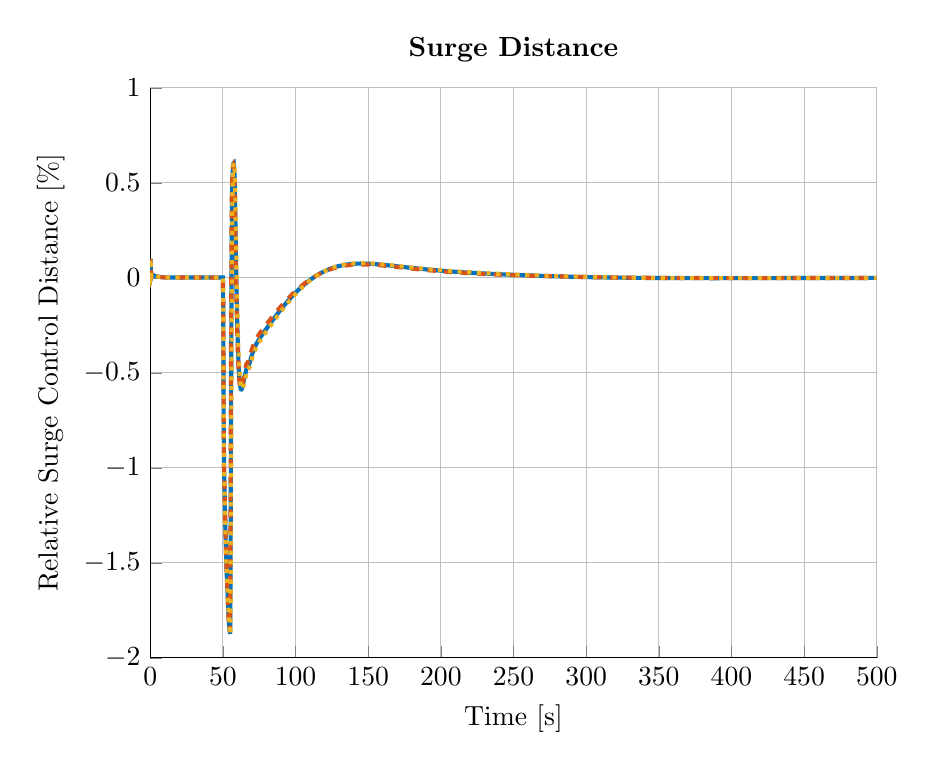
\begin{tikzpicture}

\begin{axis}[%
width=0.761\linewidth,
height=0.597\linewidth,
at={(0\linewidth,0\linewidth)},
scale only axis,
xmin=0,
xmax=500,
xlabel={Time [s]},
xmajorgrids,
ymin=-2,
ymax=1,
ylabel={Relative Surge Control Distance [\%]},
ymajorgrids,
axis background/.style={fill=white},
title style={font=\bfseries},
title={Surge Distance},
axis x line*=bottom,
axis y line*=left
]
\addplot [color=mycolor1,solid,line width=1.5pt,forget plot]
  table[row sep=crcr]{%
0	0.0693700000000002\\
0.25	0.0990399999999996\\
0.5	0.0265199999999997\\
0.75	0.00999999999999979\\
1	0.0180300000000004\\
1.25	0.0180600000000002\\
1.5	0.01539\\
1.75	0.0145999999999997\\
2	0.0142600000000002\\
2.25	0.0136000000000003\\
2.5	0.0129200000000003\\
2.75	0.0122999999999998\\
3	0.0117099999999999\\
3.25	0.0111299999999996\\
3.5	0.0105599999999999\\
3.75	0.0100199999999999\\
4	0.00949000000000044\\
4.25	0.00898999999999983\\
4.5	0.00849999999999973\\
4.75	0.00804000000000027\\
5	0.00759000000000043\\
5.25	0.00717000000000034\\
5.5	0.00677000000000039\\
5.75	0.00638999999999967\\
6	0.00602999999999998\\
6.25	0.00569000000000042\\
6.5	0.00535999999999959\\
6.75	0.00506000000000029\\
7	0.00478000000000023\\
7.25	0.00450999999999979\\
7.5	0.00426000000000037\\
7.75	0.0040300000000002\\
8	0.00380999999999965\\
8.25	0.00361000000000011\\
8.5	0.0034200000000002\\
8.75	0.00325000000000042\\
9	0.00309000000000026\\
9.25	0.00293999999999972\\
9.5	0.0028100000000002\\
9.75	0.00267999999999979\\
10	0.00257000000000041\\
10.25	0.00246999999999975\\
10.5	0.00236999999999998\\
10.75	0.00229000000000035\\
11	0.00220999999999982\\
11.25	0.00215000000000032\\
11.5	0.00208999999999993\\
11.75	0.00203000000000042\\
12	0.00197999999999965\\
12.25	0.00194000000000027\\
12.5	0.00190000000000001\\
12.75	0.00187000000000026\\
13	0.00185000000000013\\
13.25	0.00182000000000038\\
13.5	0.00180000000000025\\
13.75	0.00178999999999974\\
14	0.00178000000000011\\
14.25	0.00176999999999961\\
14.5	0.00175999999999998\\
14.75	0.00175000000000036\\
15	0.00175000000000036\\
15.25	0.00175000000000036\\
15.5	0.00175000000000036\\
15.75	0.00175000000000036\\
16	0.00175999999999998\\
16.25	0.00175999999999998\\
16.5	0.00175999999999998\\
16.75	0.00176999999999961\\
17	0.00178000000000011\\
17.25	0.00178000000000011\\
17.5	0.00178999999999974\\
17.75	0.00180000000000025\\
18	0.00180000000000025\\
18.25	0.00180999999999987\\
18.5	0.00182000000000038\\
18.75	0.00183\\
19	0.00183\\
19.25	0.00183999999999962\\
19.5	0.00185000000000013\\
19.75	0.00185000000000013\\
20	0.00185999999999975\\
20.25	0.00187000000000026\\
20.5	0.00187000000000026\\
20.75	0.00187999999999988\\
21	0.00187999999999988\\
21.25	0.00189000000000039\\
21.5	0.00189000000000039\\
21.75	0.00190000000000001\\
22	0.00190000000000001\\
22.25	0.00190000000000001\\
22.5	0.00190000000000001\\
22.75	0.00190999999999963\\
23	0.00190999999999963\\
23.25	0.00190999999999963\\
23.5	0.00190999999999963\\
23.75	0.00190999999999963\\
24	0.00190999999999963\\
24.25	0.00190999999999963\\
24.5	0.00190999999999963\\
24.75	0.00190999999999963\\
25	0.00190999999999963\\
25.25	0.00190999999999963\\
25.5	0.00190999999999963\\
25.75	0.00190999999999963\\
26	0.00190999999999963\\
26.25	0.00190000000000001\\
26.5	0.00190000000000001\\
26.75	0.00190000000000001\\
27	0.00190000000000001\\
27.25	0.00190000000000001\\
27.5	0.00189000000000039\\
27.75	0.00189000000000039\\
28	0.00189000000000039\\
28.25	0.00187999999999988\\
28.5	0.00187999999999988\\
28.75	0.00187999999999988\\
29	0.00187000000000026\\
29.25	0.00187000000000026\\
29.5	0.00187000000000026\\
29.75	0.00185999999999975\\
30	0.00185999999999975\\
30.25	0.00185999999999975\\
30.5	0.00185000000000013\\
30.75	0.00185000000000013\\
31	0.00183999999999962\\
31.25	0.00183999999999962\\
31.5	0.00183999999999962\\
31.75	0.00183\\
32	0.00183\\
32.25	0.00183\\
32.5	0.00182000000000038\\
32.75	0.00182000000000038\\
33	0.00180999999999987\\
33.25	0.00180999999999987\\
33.5	0.00180999999999987\\
33.75	0.00180000000000025\\
34	0.00180000000000025\\
34.25	0.00180000000000025\\
34.5	0.00178999999999974\\
34.75	0.00178999999999974\\
35	0.00178999999999974\\
35.25	0.00178000000000011\\
35.5	0.00178000000000011\\
35.75	0.00178000000000011\\
36	0.00176999999999961\\
36.25	0.00176999999999961\\
36.5	0.00176999999999961\\
36.75	0.00175999999999998\\
37	0.00175999999999998\\
37.25	0.00175999999999998\\
37.5	0.00175000000000036\\
37.75	0.00175000000000036\\
38	0.00175000000000036\\
38.25	0.00173999999999985\\
38.5	0.00173999999999985\\
38.75	0.00173999999999985\\
39	0.00173999999999985\\
39.25	0.00173000000000023\\
39.5	0.00173000000000023\\
39.75	0.00173000000000023\\
40	0.00171999999999972\\
40.25	0.00171999999999972\\
40.5	0.00171999999999972\\
40.75	0.00171999999999972\\
41	0.0017100000000001\\
41.25	0.0017100000000001\\
41.5	0.0017100000000001\\
41.75	0.0017100000000001\\
42	0.00169999999999959\\
42.25	0.00169999999999959\\
42.5	0.00169999999999959\\
42.75	0.00169999999999959\\
43	0.00169999999999959\\
43.25	0.00168999999999997\\
43.5	0.00168999999999997\\
43.75	0.00168999999999997\\
44	0.00168999999999997\\
44.25	0.00168000000000035\\
44.5	0.00168000000000035\\
44.75	0.00168000000000035\\
45	0.00168000000000035\\
45.25	0.00168000000000035\\
45.5	0.00166999999999984\\
45.75	0.00166999999999984\\
46	0.00166999999999984\\
46.25	0.00166999999999984\\
46.5	0.00166999999999984\\
46.75	0.00166999999999984\\
47	0.00166000000000022\\
47.25	0.00166000000000022\\
47.5	0.00166000000000022\\
47.75	0.00166000000000022\\
48	0.00166000000000022\\
48.25	0.00164999999999971\\
48.5	0.00164999999999971\\
48.75	0.00164999999999971\\
49	0.00164999999999971\\
49.25	0.00164999999999971\\
49.5	0.00164999999999971\\
49.75	0.00164999999999971\\
50	0.00164000000000009\\
50.25	-0.15753\\
50.5	-0.67415\\
50.75	-0.97497\\
51	-1.0645\\
51.25	-1.14641\\
51.5	-1.24849\\
51.75	-1.33687\\
52	-1.40864\\
52.25	-1.47242\\
52.5	-1.52977\\
52.75	-1.57967\\
53	-1.62275\\
53.25	-1.66337\\
53.5	-1.70892\\
53.75	-1.75344\\
54	-1.79266\\
54.25	-1.82558\\
54.5	-1.84848\\
54.75	-1.8633\\
55	-1.87315\\
55.25	-1.55099\\
55.5	-0.9513\\
55.75	-0.43173\\
56	0.0882399999999999\\
56.25	0.40155\\
56.5	0.50932\\
56.75	0.55751\\
57	0.58834\\
57.25	0.60285\\
57.5	0.60479\\
57.75	0.58705\\
58	0.53864\\
58.25	0.45678\\
58.5	0.34801\\
58.75	0.22685\\
59	0.10656\\
59.25	-0.00595999999999997\\
59.5	-0.10799\\
59.75	-0.19842\\
60	-0.27716\\
60.25	-0.34473\\
60.5	-0.40193\\
60.75	-0.4496\\
61	-0.48859\\
61.25	-0.51978\\
61.5	-0.54401\\
61.75	-0.5621\\
62	-0.57478\\
62.25	-0.58273\\
62.5	-0.58661\\
62.75	-0.58702\\
63	-0.58451\\
63.25	-0.57963\\
63.5	-0.57288\\
63.75	-0.56472\\
64	-0.55556\\
64.25	-0.54581\\
64.5	-0.53597\\
64.75	-0.52762\\
65	-0.51988\\
65.25	-0.51137\\
65.5	-0.50264\\
65.75	-0.49434\\
66	-0.48649\\
66.25	-0.47898\\
66.5	-0.47203\\
66.75	-0.46869\\
67	-0.46901\\
67.25	-0.4685\\
67.5	-0.46562\\
67.75	-0.46131\\
68	-0.45617\\
68.25	-0.45034\\
68.5	-0.44403\\
68.75	-0.43748\\
69	-0.43085\\
69.25	-0.42422\\
69.5	-0.41764\\
69.75	-0.41121\\
70	-0.40499\\
70.25	-0.399\\
70.5	-0.39325\\
70.75	-0.38777\\
71	-0.38253\\
71.25	-0.37753\\
71.5	-0.37276\\
71.75	-0.36821\\
72	-0.36386\\
72.25	-0.3597\\
72.5	-0.3557\\
72.75	-0.35187\\
73	-0.34817\\
73.25	-0.3446\\
73.5	-0.34114\\
73.75	-0.33779\\
74	-0.33453\\
74.25	-0.33134\\
74.5	-0.32823\\
74.75	-0.32518\\
75	-0.32218\\
75.25	-0.31923\\
75.5	-0.31633\\
75.75	-0.31346\\
76	-0.31062\\
76.25	-0.3078\\
76.5	-0.30502\\
76.75	-0.30225\\
77	-0.2995\\
77.25	-0.29676\\
77.5	-0.29404\\
77.75	-0.29132\\
78	-0.28862\\
78.25	-0.28592\\
78.5	-0.28324\\
78.75	-0.28055\\
79	-0.27788\\
79.25	-0.2752\\
79.5	-0.27253\\
79.75	-0.26987\\
80	-0.26721\\
80.25	-0.26455\\
80.5	-0.2619\\
80.75	-0.25925\\
81	-0.2566\\
81.25	-0.25396\\
81.5	-0.25132\\
81.75	-0.24869\\
82	-0.24606\\
82.25	-0.24343\\
82.5	-0.24081\\
82.75	-0.23819\\
83	-0.23558\\
83.25	-0.23297\\
83.5	-0.23037\\
83.75	-0.22777\\
84	-0.22518\\
84.25	-0.22259\\
84.5	-0.22001\\
84.75	-0.21744\\
85	-0.21487\\
85.25	-0.21231\\
85.5	-0.20976\\
85.75	-0.20721\\
86	-0.20467\\
86.25	-0.20214\\
86.5	-0.19962\\
86.75	-0.1971\\
87	-0.19459\\
87.25	-0.19209\\
87.5	-0.1896\\
87.75	-0.18712\\
88	-0.18465\\
88.25	-0.18218\\
88.5	-0.17972\\
88.75	-0.17728\\
89	-0.17484\\
89.25	-0.17241\\
89.5	-0.16999\\
89.75	-0.16758\\
90	-0.16518\\
90.25	-0.16279\\
90.5	-0.16041\\
90.75	-0.15804\\
91	-0.15568\\
91.25	-0.15333\\
91.5	-0.15099\\
91.75	-0.14866\\
92	-0.14634\\
92.25	-0.14403\\
92.5	-0.14173\\
92.75	-0.13944\\
93	-0.13717\\
93.25	-0.1349\\
93.5	-0.13265\\
93.75	-0.1304\\
94	-0.12817\\
94.25	-0.12595\\
94.5	-0.12374\\
94.75	-0.12154\\
95	-0.11936\\
95.25	-0.11718\\
95.5	-0.11502\\
95.75	-0.11287\\
96	-0.11073\\
96.25	-0.1086\\
96.5	-0.10648\\
96.75	-0.10438\\
97	-0.10229\\
97.25	-0.10021\\
97.5	-0.0981399999999999\\
97.75	-0.0960900000000002\\
98	-0.0940399999999997\\
98.25	-0.0920100000000001\\
98.5	-0.0899900000000002\\
98.75	-0.0879899999999996\\
99	-0.0859899999999998\\
99.25	-0.0840100000000001\\
99.5	-0.0820400000000001\\
99.75	-0.0800799999999997\\
100	-0.0781400000000003\\
100.25	-0.0762099999999997\\
100.5	-0.0742900000000004\\
100.75	-0.0723799999999999\\
101	-0.0704900000000004\\
101.25	-0.0686099999999996\\
101.5	-0.0667400000000002\\
101.75	-0.0648900000000001\\
102	-0.0630499999999996\\
102.25	-0.0612199999999996\\
102.5	-0.0594000000000001\\
102.75	-0.0575999999999999\\
103	-0.0558100000000001\\
103.25	-0.05403\\
103.5	-0.05227\\
103.75	-0.0505199999999997\\
104	-0.0487799999999998\\
104.25	-0.0470499999999996\\
104.5	-0.0453400000000004\\
104.75	-0.0436399999999999\\
105	-0.0419600000000004\\
105.25	-0.0402899999999997\\
105.5	-0.0386300000000004\\
105.75	-0.0369799999999998\\
106	-0.0353500000000002\\
106.25	-0.0337300000000003\\
106.5	-0.0321199999999999\\
106.75	-0.0305299999999997\\
107	-0.02895\\
107.25	-0.02738\\
107.5	-0.02583\\
107.75	-0.0242899999999997\\
108	-0.0227599999999999\\
108.25	-0.0212500000000002\\
108.5	-0.0197500000000002\\
108.75	-0.0182599999999997\\
109	-0.0167799999999998\\
109.25	-0.01532\\
109.5	-0.0138699999999998\\
109.75	-0.0124399999999998\\
110	-0.0110200000000003\\
110.25	-0.00961000000000034\\
110.5	-0.00821000000000005\\
110.75	-0.00682999999999989\\
111	-0.00546000000000024\\
111.25	-0.00410999999999984\\
111.5	-0.00276999999999994\\
111.75	-0.00143999999999966\\
112	-0.000119999999999898\\
112.25	0.00117999999999974\\
112.5	0.00246999999999975\\
112.75	0.00375000000000014\\
113	0.00502000000000002\\
113.25	0.00626999999999978\\
113.5	0.00750999999999991\\
113.75	0.0087299999999999\\
114	0.00994000000000028\\
114.25	0.0111400000000001\\
114.5	0.0123300000000004\\
114.75	0.0134999999999996\\
115	0.0146600000000001\\
115.25	0.0158100000000001\\
115.5	0.0169499999999996\\
115.75	0.0180699999999998\\
116	0.0191800000000004\\
116.25	0.0202799999999996\\
116.5	0.0213599999999996\\
116.75	0.0224299999999999\\
117	0.0234899999999998\\
117.25	0.02454\\
117.5	0.0255700000000001\\
117.75	0.0265899999999997\\
118	0.0275999999999996\\
118.25	0.0286\\
118.5	0.0295800000000002\\
118.75	0.0305600000000004\\
119	0.0315200000000004\\
119.25	0.0324600000000004\\
119.5	0.0334000000000003\\
119.75	0.0343200000000001\\
120	0.0352300000000003\\
120.25	0.03613\\
120.5	0.0370200000000001\\
120.75	0.03789\\
121	0.0387599999999999\\
121.25	0.0396099999999997\\
121.5	0.0404499999999999\\
121.75	0.0412800000000004\\
122	0.04209\\
122.25	0.0429000000000004\\
122.5	0.0436899999999998\\
122.75	0.0444699999999996\\
123	0.0452399999999997\\
123.25	0.0460000000000003\\
123.5	0.0467399999999998\\
123.75	0.0474800000000002\\
124	0.0481999999999996\\
124.25	0.0489100000000002\\
124.5	0.0496100000000004\\
124.75	0.0503\\
125	0.05098\\
125.25	0.0516500000000004\\
125.5	0.0523100000000003\\
125.75	0.0529500000000001\\
126	0.0535899999999998\\
126.25	0.0542100000000003\\
126.5	0.0548299999999999\\
126.75	0.0554300000000003\\
127	0.0560200000000002\\
127.25	0.0566000000000004\\
127.5	0.0571799999999998\\
127.75	0.0577399999999999\\
128	0.0582900000000004\\
128.25	0.0588300000000004\\
128.5	0.0593599999999999\\
128.75	0.0598799999999997\\
129	0.0603899999999999\\
129.25	0.0608899999999997\\
129.5	0.0613799999999998\\
129.75	0.0618600000000002\\
130	0.0623199999999997\\
130.25	0.0627899999999997\\
130.5	0.0632400000000004\\
130.75	0.0636799999999997\\
131	0.0641100000000003\\
131.25	0.0645300000000004\\
131.5	0.06494\\
131.75	0.06534\\
132	0.0657399999999999\\
132.25	0.0661199999999997\\
132.5	0.0664999999999996\\
132.75	0.0668600000000001\\
133	0.0672199999999998\\
133.25	0.0675699999999999\\
133.5	0.0679100000000004\\
133.75	0.0682400000000003\\
134	0.0685599999999997\\
134.25	0.0688800000000001\\
134.5	0.0691800000000002\\
134.75	0.0694800000000004\\
135	0.0697700000000001\\
135.25	0.0700500000000002\\
135.5	0.0703199999999997\\
135.75	0.0705799999999996\\
136	0.0708399999999996\\
136.25	0.0710800000000003\\
136.5	0.0713200000000001\\
136.75	0.0715500000000002\\
137	0.0717800000000004\\
137.25	0.0719900000000004\\
137.5	0.0721999999999996\\
137.75	0.0724\\
138	0.0725899999999999\\
138.25	0.0727799999999998\\
138.5	0.0729600000000001\\
138.75	0.0731299999999999\\
139	0.0732900000000001\\
139.25	0.0734500000000002\\
139.5	0.0735999999999999\\
139.75	0.0737399999999999\\
140	0.0738799999999999\\
140.25	0.0740100000000004\\
140.5	0.0741300000000003\\
140.75	0.0742500000000001\\
141	0.0743600000000004\\
141.25	0.0744600000000002\\
141.5	0.07456\\
141.75	0.0746500000000001\\
142	0.0747299999999997\\
142.25	0.0748100000000003\\
142.5	0.0748800000000003\\
142.75	0.0749399999999998\\
143	0.0750000000000002\\
143.25	0.0750599999999997\\
143.5	0.0750999999999999\\
143.75	0.0751499999999998\\
144	0.0751799999999996\\
144.25	0.0752100000000002\\
144.5	0.07524\\
144.75	0.0752600000000001\\
145	0.0752699999999997\\
145.25	0.0752800000000002\\
145.5	0.0752899999999999\\
145.75	0.0752899999999999\\
146	0.0752800000000002\\
146.25	0.0752699999999997\\
146.5	0.0752499999999996\\
146.75	0.0752300000000004\\
147	0.0752100000000002\\
147.25	0.0751799999999996\\
147.5	0.0751400000000002\\
147.75	0.0750999999999999\\
148	0.0750599999999997\\
148.25	0.0750099999999998\\
148.5	0.0749599999999999\\
148.75	0.0749000000000004\\
149	0.07484\\
149.25	0.07477\\
149.5	0.0747\\
149.75	0.07463\\
150	0.0745500000000003\\
150.25	0.0744699999999998\\
150.5	0.0743900000000002\\
150.75	0.0743\\
151	0.0742099999999999\\
151.25	0.0741100000000001\\
151.5	0.0740100000000004\\
151.75	0.0739099999999997\\
152	0.0738000000000003\\
152.25	0.07369\\
152.5	0.0735799999999998\\
152.75	0.0734599999999999\\
153	0.0733499999999996\\
153.25	0.0732200000000001\\
153.5	0.0731000000000002\\
153.75	0.0729699999999998\\
154	0.0728400000000002\\
154.25	0.0727000000000002\\
154.5	0.0725699999999998\\
154.75	0.0724299999999998\\
155	0.0722899999999997\\
155.25	0.0721400000000001\\
155.5	0.0719900000000004\\
155.75	0.0718399999999999\\
156	0.0716900000000003\\
156.25	0.0715399999999997\\
156.5	0.0713800000000004\\
156.75	0.0712200000000003\\
157	0.0710600000000001\\
157.25	0.0709\\
157.5	0.0707300000000002\\
157.75	0.0705600000000004\\
158	0.0704000000000002\\
158.25	0.0702199999999999\\
158.5	0.0700500000000002\\
158.75	0.0698800000000004\\
159	0.0697000000000001\\
159.25	0.0695199999999998\\
159.5	0.0693400000000004\\
159.75	0.0691600000000001\\
160	0.0689700000000002\\
160.25	0.0687899999999999\\
160.5	0.0686\\
160.75	0.0684100000000001\\
161	0.0682200000000002\\
161.25	0.0680300000000003\\
161.5	0.0678400000000003\\
161.75	0.0676500000000004\\
162	0.06745\\
162.25	0.0672600000000001\\
162.5	0.0670599999999997\\
162.75	0.0668600000000001\\
163	0.0666599999999997\\
163.25	0.0664600000000002\\
163.5	0.0662599999999998\\
163.75	0.0660600000000002\\
164	0.0658500000000002\\
164.25	0.0656499999999998\\
164.5	0.0654500000000002\\
164.75	0.0652400000000002\\
165	0.0650300000000001\\
165.25	0.0648299999999997\\
165.5	0.0646199999999997\\
165.75	0.0644099999999996\\
166	0.0641999999999996\\
166.25	0.0639900000000004\\
166.5	0.0637800000000004\\
166.75	0.0635700000000003\\
167	0.0633600000000003\\
167.25	0.0631500000000003\\
167.5	0.0629299999999997\\
167.75	0.0627199999999997\\
168	0.0625099999999996\\
168.25	0.06229\\
168.5	0.0620799999999999\\
168.75	0.0618699999999999\\
169	0.0616500000000002\\
169.25	0.0614400000000002\\
169.5	0.0612199999999996\\
169.75	0.0610099999999996\\
170	0.0607899999999999\\
170.25	0.0605799999999999\\
170.5	0.0603600000000002\\
170.75	0.0601500000000001\\
171	0.0599299999999996\\
171.25	0.0597200000000004\\
171.5	0.0594999999999999\\
171.75	0.0592800000000002\\
172	0.0590700000000002\\
172.25	0.0588499999999996\\
172.5	0.0586399999999996\\
172.75	0.0584199999999999\\
173	0.0582099999999999\\
173.25	0.0579900000000002\\
173.5	0.0577800000000002\\
173.75	0.0575599999999996\\
174	0.0573499999999996\\
174.25	0.0571299999999999\\
174.5	0.0569199999999999\\
174.75	0.0567099999999998\\
175	0.0564900000000002\\
175.25	0.0562800000000001\\
175.5	0.0560700000000001\\
175.75	0.0558500000000004\\
176	0.0556400000000004\\
176.25	0.0554300000000003\\
176.5	0.0552200000000003\\
176.75	0.0549999999999997\\
177	0.0547899999999997\\
177.25	0.0545799999999996\\
177.5	0.0543699999999996\\
177.75	0.0541600000000004\\
178	0.0539500000000004\\
178.25	0.0537400000000003\\
178.5	0.0535300000000003\\
178.75	0.0533299999999999\\
179	0.0531199999999998\\
179.25	0.0529099999999998\\
179.5	0.0526999999999997\\
179.75	0.0525000000000002\\
180	0.0522900000000002\\
180.25	0.0520899999999997\\
180.5	0.0518799999999997\\
180.75	0.0516800000000002\\
181	0.0514700000000001\\
181.25	0.0512699999999997\\
181.5	0.0510700000000002\\
181.75	0.0508699999999997\\
182	0.0506700000000002\\
182.25	0.0504600000000002\\
182.5	0.0502599999999997\\
182.75	0.0500600000000002\\
183	0.0498700000000003\\
183.25	0.0496699999999999\\
183.5	0.0494700000000003\\
183.75	0.0492699999999999\\
184	0.04908\\
184.25	0.0488799999999996\\
184.5	0.0486800000000001\\
184.75	0.0484900000000001\\
185	0.0482899999999997\\
185.25	0.0480999999999998\\
185.5	0.0479099999999999\\
185.75	0.04772\\
186	0.0475199999999996\\
186.25	0.0473299999999997\\
186.5	0.0471399999999997\\
186.75	0.0469499999999998\\
187	0.0467599999999999\\
187.25	0.0465799999999996\\
187.5	0.0463899999999997\\
187.75	0.0461999999999998\\
188	0.0460099999999999\\
188.25	0.0458299999999996\\
188.5	0.0456399999999997\\
188.75	0.0454600000000003\\
189	0.04528\\
189.25	0.0450900000000001\\
189.5	0.0449099999999998\\
189.75	0.0447300000000004\\
190	0.0445500000000001\\
190.25	0.0443699999999998\\
190.5	0.0441900000000004\\
190.75	0.0440100000000001\\
191	0.0438299999999998\\
191.25	0.0436500000000004\\
191.5	0.0434799999999997\\
191.75	0.0433000000000003\\
192	0.0431299999999997\\
192.25	0.0429500000000003\\
192.5	0.0427799999999996\\
192.75	0.0426000000000002\\
193	0.0424300000000004\\
193.25	0.0422599999999997\\
193.5	0.04209\\
193.75	0.0419200000000002\\
194	0.0417500000000004\\
194.25	0.0415799999999997\\
194.5	0.0414099999999999\\
194.75	0.0412400000000002\\
195	0.0410700000000004\\
195.25	0.0409100000000002\\
195.5	0.0407400000000004\\
195.75	0.0405699999999998\\
196	0.0404099999999996\\
196.25	0.0402399999999998\\
196.5	0.0400799999999997\\
196.75	0.0399200000000004\\
197	0.0397600000000002\\
197.25	0.0396000000000001\\
197.5	0.0394300000000003\\
197.75	0.0392700000000001\\
198	0.03911\\
198.25	0.0389600000000003\\
198.5	0.0388000000000002\\
198.75	0.03864\\
199	0.0384799999999998\\
199.25	0.0383300000000002\\
199.5	0.03817\\
199.75	0.0380200000000004\\
200	0.0378600000000002\\
200.25	0.0377099999999997\\
200.5	0.0375500000000004\\
200.75	0.0373999999999999\\
201	0.0372500000000002\\
201.25	0.0370999999999997\\
201.5	0.03695\\
201.75	0.0368000000000004\\
202	0.0366499999999998\\
202.25	0.0365000000000002\\
202.5	0.0363499999999997\\
202.75	0.0362\\
203	0.03606\\
203.25	0.0359100000000003\\
203.5	0.0357599999999998\\
203.75	0.0356199999999998\\
204	0.0354700000000001\\
204.25	0.0353300000000001\\
204.5	0.0351900000000001\\
204.75	0.0350400000000004\\
205	0.0349000000000004\\
205.25	0.0347600000000003\\
205.5	0.0346200000000003\\
205.75	0.0344800000000003\\
206	0.0343400000000003\\
206.25	0.0342000000000002\\
206.5	0.0340600000000002\\
206.75	0.0339200000000002\\
207	0.0337800000000001\\
207.25	0.0336400000000001\\
207.5	0.0335099999999997\\
207.75	0.0333699999999997\\
208	0.0332400000000002\\
208.25	0.0331000000000001\\
208.5	0.0329699999999997\\
208.75	0.0328299999999997\\
209	0.0327000000000002\\
209.25	0.0325600000000001\\
209.5	0.0324299999999997\\
209.75	0.0323000000000002\\
210	0.0321699999999998\\
210.25	0.0320400000000003\\
210.5	0.0319099999999999\\
210.75	0.0317800000000004\\
211	0.03165\\
211.25	0.0315200000000004\\
211.5	0.03139\\
211.75	0.0312599999999996\\
212	0.0311300000000001\\
212.25	0.0310100000000002\\
212.5	0.0308799999999998\\
212.75	0.0307500000000003\\
213	0.0306300000000004\\
213.25	0.0305\\
213.5	0.0303800000000001\\
213.75	0.0302499999999997\\
214	0.0301299999999998\\
214.25	0.0300099999999999\\
214.5	0.0298800000000004\\
214.75	0.0297599999999996\\
215	0.0296399999999997\\
215.25	0.0295199999999998\\
215.5	0.0293900000000002\\
215.75	0.0292700000000004\\
216	0.0291499999999996\\
216.25	0.0290299999999997\\
216.5	0.0289099999999998\\
216.75	0.0288000000000004\\
217	0.0286799999999996\\
217.25	0.0285599999999997\\
217.5	0.0284399999999998\\
217.75	0.0283199999999999\\
218	0.0282099999999996\\
218.25	0.0280899999999997\\
218.5	0.0279699999999998\\
218.75	0.0278600000000004\\
219	0.0277399999999997\\
219.25	0.0276300000000003\\
219.5	0.0275100000000004\\
219.75	0.0274000000000001\\
220	0.0272899999999998\\
220.25	0.0271699999999999\\
220.5	0.0270599999999996\\
220.75	0.0269500000000003\\
221	0.02684\\
221.25	0.0267200000000001\\
221.5	0.0266099999999998\\
221.75	0.0265000000000004\\
222	0.0263900000000001\\
222.25	0.0262799999999999\\
222.5	0.0261699999999996\\
222.75	0.0260600000000002\\
223	0.0259499999999999\\
223.25	0.0258399999999996\\
223.5	0.0257399999999999\\
223.75	0.0256299999999996\\
224	0.0255200000000002\\
224.25	0.0254099999999999\\
224.5	0.0253100000000002\\
224.75	0.0251999999999999\\
225	0.0250899999999996\\
225.25	0.0249899999999998\\
225.5	0.0248799999999996\\
225.75	0.0247799999999998\\
226	0.0246700000000004\\
226.25	0.0245699999999998\\
226.5	0.0244600000000004\\
226.75	0.0243599999999997\\
227	0.0242599999999999\\
227.25	0.0241499999999997\\
227.5	0.0240499999999999\\
227.75	0.0239500000000001\\
228	0.0238500000000004\\
228.25	0.0237499999999997\\
228.5	0.0236400000000003\\
228.75	0.0235399999999997\\
229	0.0234399999999999\\
229.25	0.0233400000000001\\
229.5	0.0232400000000004\\
229.75	0.0231399999999997\\
230	0.0230399999999999\\
230.25	0.0229400000000002\\
230.5	0.0228400000000004\\
230.75	0.0227399999999998\\
231	0.0226499999999996\\
231.25	0.0225499999999998\\
231.5	0.0224500000000001\\
231.75	0.0223500000000003\\
232	0.0222600000000002\\
232.25	0.0221600000000004\\
232.5	0.0220599999999997\\
232.75	0.0219699999999996\\
233	0.0218699999999998\\
233.25	0.0217700000000001\\
233.5	0.0216799999999999\\
233.75	0.0215800000000002\\
234	0.02149\\
234.25	0.0213999999999999\\
234.5	0.0213000000000001\\
234.75	0.02121\\
235	0.0211100000000002\\
235.25	0.02102\\
235.5	0.0209299999999999\\
235.75	0.0208300000000001\\
236	0.02074\\
236.25	0.0206499999999998\\
236.5	0.0205599999999997\\
236.75	0.0204700000000004\\
237	0.0203699999999998\\
237.25	0.0202799999999996\\
237.5	0.0201900000000004\\
237.75	0.0201000000000002\\
238	0.0200100000000001\\
238.25	0.0199199999999999\\
238.5	0.0198299999999998\\
238.75	0.0197399999999996\\
239	0.0196500000000004\\
239.25	0.0195600000000002\\
239.5	0.0194700000000001\\
239.75	0.0193899999999996\\
240	0.0193000000000003\\
240.25	0.0192100000000002\\
240.5	0.01912\\
240.75	0.0190299999999999\\
241	0.0189500000000002\\
241.25	0.0188600000000001\\
241.5	0.01877\\
241.75	0.0186900000000003\\
242	0.0186000000000002\\
242.25	0.01851\\
242.5	0.0184300000000004\\
242.75	0.0183400000000002\\
243	0.0182599999999997\\
243.25	0.0181699999999996\\
243.5	0.0180899999999999\\
243.75	0.0179999999999998\\
244	0.0179200000000002\\
244.25	0.01783\\
244.5	0.0177500000000004\\
244.75	0.0176699999999999\\
245	0.0175799999999997\\
245.25	0.0175000000000001\\
245.5	0.0174200000000004\\
245.75	0.0173300000000003\\
246	0.0172499999999998\\
246.25	0.0171700000000001\\
246.5	0.0170899999999996\\
246.75	0.01701\\
247	0.0169199999999998\\
247.25	0.0168400000000002\\
247.5	0.0167599999999997\\
247.75	0.01668\\
248	0.0166000000000004\\
248.25	0.0165199999999999\\
248.5	0.0164400000000002\\
248.75	0.0163599999999997\\
249	0.0162800000000001\\
249.25	0.0162000000000004\\
249.5	0.0161199999999999\\
249.75	0.0160400000000003\\
250	0.0159599999999998\\
250.25	0.0158899999999997\\
250.5	0.0158100000000001\\
250.75	0.0157299999999996\\
251	0.0156499999999999\\
251.25	0.0155700000000003\\
251.5	0.0155000000000003\\
251.75	0.0154199999999998\\
252	0.0153400000000001\\
252.25	0.0152599999999996\\
252.5	0.0151899999999996\\
252.75	0.01511\\
253	0.0150300000000003\\
253.25	0.0149600000000003\\
253.5	0.0148799999999998\\
253.75	0.0148099999999998\\
254	0.0147300000000001\\
254.25	0.0146600000000001\\
254.5	0.0145799999999996\\
254.75	0.0145099999999996\\
255	0.0144299999999999\\
255.25	0.0143599999999999\\
255.5	0.0142800000000003\\
255.75	0.0142100000000003\\
256	0.0141400000000003\\
256.25	0.0140599999999997\\
256.5	0.0139899999999997\\
256.75	0.0139199999999997\\
257	0.0138400000000001\\
257.25	0.0137700000000001\\
257.5	0.0137\\
257.75	0.01363\\
258	0.0135500000000004\\
258.25	0.0134800000000004\\
258.5	0.0134100000000004\\
258.75	0.0133400000000004\\
259	0.0132700000000003\\
259.25	0.0132000000000003\\
259.5	0.0131300000000003\\
259.75	0.0130600000000003\\
260	0.0129900000000003\\
260.25	0.0129200000000003\\
260.5	0.0128500000000003\\
260.75	0.0127800000000002\\
261	0.0127100000000002\\
261.25	0.0126400000000002\\
261.5	0.0125700000000002\\
261.75	0.0125000000000002\\
262	0.0124300000000002\\
262.25	0.0123600000000001\\
262.5	0.0122900000000001\\
262.75	0.0122299999999997\\
263	0.0121599999999997\\
263.25	0.0120899999999997\\
263.5	0.0120199999999997\\
263.75	0.0119499999999997\\
264	0.0118900000000002\\
264.25	0.0118200000000002\\
264.5	0.0117500000000001\\
264.75	0.0116899999999998\\
265	0.0116199999999997\\
265.25	0.0115499999999997\\
265.5	0.0114900000000002\\
265.75	0.0114200000000002\\
266	0.0113599999999998\\
266.25	0.0112899999999998\\
266.5	0.0112300000000003\\
266.75	0.0111600000000003\\
267	0.0110999999999999\\
267.25	0.0110299999999999\\
267.5	0.0109700000000004\\
267.75	0.0109000000000004\\
268	0.01084\\
268.25	0.0107699999999999\\
268.5	0.0107100000000004\\
268.75	0.01065\\
269	0.01058\\
269.25	0.0105199999999996\\
269.5	0.0104600000000001\\
269.75	0.0103999999999997\\
270	0.0103299999999997\\
270.25	0.0102700000000002\\
270.5	0.0102099999999998\\
270.75	0.0101500000000003\\
271	0.0100800000000003\\
271.25	0.0100199999999999\\
271.5	0.00996000000000041\\
271.75	0.00990000000000002\\
272	0.00983999999999963\\
272.25	0.00978000000000012\\
272.5	0.00971999999999973\\
272.75	0.00966000000000022\\
273	0.00959999999999983\\
273.25	0.00954000000000033\\
273.5	0.00947999999999993\\
273.75	0.00942000000000043\\
274	0.00936000000000003\\
274.25	0.00929999999999964\\
274.5	0.00924000000000014\\
274.75	0.00917999999999974\\
275	0.00912000000000024\\
275.25	0.00905999999999985\\
275.5	0.00900999999999996\\
275.75	0.00894999999999957\\
276	0.00889000000000006\\
276.25	0.00882999999999967\\
276.5	0.00877000000000017\\
276.75	0.00872000000000028\\
277	0.00865999999999989\\
277.25	0.00860000000000039\\
277.5	0.00854999999999961\\
277.75	0.00849000000000011\\
278	0.00842999999999972\\
278.25	0.00837999999999983\\
278.5	0.00832000000000033\\
278.75	0.00825999999999993\\
279	0.00821000000000005\\
279.25	0.00814999999999966\\
279.5	0.00809999999999977\\
279.75	0.00804000000000027\\
280	0.00799000000000039\\
280.25	0.00792999999999999\\
280.5	0.00788000000000011\\
280.75	0.00781999999999972\\
281	0.00776999999999983\\
281.25	0.00771999999999995\\
281.5	0.00765999999999956\\
281.75	0.00760999999999967\\
282	0.00755000000000017\\
282.25	0.00750000000000028\\
282.5	0.0074500000000004\\
282.75	0.00739000000000001\\
283	0.00734000000000012\\
283.25	0.00729000000000024\\
283.5	0.00724000000000036\\
283.75	0.00717999999999996\\
284	0.00713000000000008\\
284.25	0.0070800000000002\\
284.5	0.00703000000000031\\
284.75	0.00698000000000043\\
285	0.00692999999999966\\
285.25	0.00687999999999978\\
285.5	0.00682000000000027\\
285.75	0.00677000000000039\\
286	0.00671999999999962\\
286.25	0.00666999999999973\\
286.5	0.00661999999999985\\
286.75	0.00656999999999996\\
287	0.00652000000000008\\
287.25	0.0064700000000002\\
287.5	0.00642000000000031\\
287.75	0.00637000000000043\\
288	0.00631999999999966\\
288.25	0.00628000000000029\\
288.5	0.0062300000000004\\
288.75	0.00617999999999963\\
289	0.00612999999999975\\
289.25	0.00607999999999986\\
289.5	0.00602999999999998\\
289.75	0.00598999999999972\\
290	0.00593999999999983\\
290.25	0.00588999999999995\\
290.5	0.00584000000000007\\
290.75	0.00579999999999981\\
291	0.00574999999999992\\
291.25	0.00570000000000004\\
291.5	0.00565999999999978\\
291.75	0.00560999999999989\\
292	0.00556000000000001\\
292.25	0.00551999999999975\\
292.5	0.00546999999999986\\
292.75	0.00541999999999998\\
293	0.00537999999999972\\
293.25	0.00532999999999983\\
293.5	0.00528999999999957\\
293.75	0.00523999999999969\\
294	0.00520000000000032\\
294.25	0.00515000000000043\\
294.5	0.00511000000000017\\
294.75	0.00506999999999991\\
295	0.00502000000000002\\
295.25	0.00497999999999976\\
295.5	0.00492999999999988\\
295.75	0.00488999999999962\\
296	0.00485000000000024\\
296.25	0.00480000000000036\\
296.5	0.0047600000000001\\
296.75	0.00471999999999984\\
297	0.00466999999999995\\
297.25	0.00462999999999969\\
297.5	0.00459000000000032\\
297.75	0.00455000000000005\\
298	0.00450999999999979\\
298.25	0.00445999999999991\\
298.5	0.00441999999999965\\
298.75	0.00438000000000027\\
299	0.00434000000000001\\
299.25	0.00429999999999975\\
299.5	0.00426000000000037\\
299.75	0.00422000000000011\\
300	0.00417000000000023\\
300.25	0.00412999999999997\\
300.5	0.0040899999999997\\
300.75	0.00405000000000033\\
301	0.00401000000000007\\
301.25	0.00396999999999981\\
301.5	0.00393000000000043\\
301.75	0.00389999999999979\\
302	0.00386000000000042\\
302.25	0.00382000000000016\\
302.5	0.00377999999999989\\
302.75	0.00373999999999963\\
303	0.00370000000000026\\
303.25	0.00366\\
303.5	0.00361999999999973\\
303.75	0.00358999999999998\\
304	0.00354999999999972\\
304.25	0.00351000000000035\\
304.5	0.00347000000000008\\
304.75	0.00342999999999982\\
305	0.00340000000000007\\
305.25	0.00335999999999981\\
305.5	0.00332000000000043\\
305.75	0.00328999999999979\\
306	0.00325000000000042\\
306.25	0.00321000000000016\\
306.5	0.0031800000000004\\
306.75	0.00314000000000014\\
307	0.00311000000000039\\
307.25	0.00307000000000013\\
307.5	0.00302999999999987\\
307.75	0.00300000000000011\\
308	0.00295999999999985\\
308.25	0.0029300000000001\\
308.5	0.00288999999999984\\
308.75	0.00286000000000008\\
309	0.00281999999999982\\
309.25	0.00279000000000007\\
309.5	0.00276000000000032\\
309.75	0.00272000000000006\\
310	0.0026900000000003\\
310.25	0.00265000000000004\\
310.5	0.00262000000000029\\
310.75	0.00258999999999965\\
311	0.00255000000000027\\
311.25	0.00251999999999963\\
311.5	0.00248999999999988\\
311.75	0.00244999999999962\\
312	0.00241999999999987\\
312.25	0.00239000000000011\\
312.5	0.00236000000000036\\
312.75	0.00232999999999972\\
313	0.00229000000000035\\
313.25	0.00225999999999971\\
313.5	0.00222999999999995\\
313.75	0.0022000000000002\\
314	0.00216999999999956\\
314.25	0.00213999999999981\\
314.5	0.00210000000000043\\
314.75	0.00206999999999979\\
315	0.00204000000000004\\
315.25	0.00201000000000029\\
315.5	0.00197999999999965\\
315.75	0.0019499999999999\\
316	0.00192000000000014\\
316.25	0.00189000000000039\\
316.5	0.00185999999999975\\
316.75	0.00183\\
317	0.00180000000000025\\
317.25	0.00176999999999961\\
317.5	0.00173999999999985\\
317.75	0.00171999999999972\\
318	0.00168999999999997\\
318.25	0.00166000000000022\\
318.5	0.00162999999999958\\
318.75	0.00159999999999982\\
319	0.00157000000000007\\
319.25	0.00154999999999994\\
319.5	0.00152000000000019\\
319.75	0.00149000000000044\\
320	0.00145999999999979\\
320.25	0.00143000000000004\\
320.5	0.00140999999999991\\
320.75	0.00138000000000016\\
321	0.00135000000000041\\
321.25	0.00133000000000028\\
321.5	0.00129999999999963\\
321.75	0.00126999999999988\\
322	0.00124999999999975\\
322.25	0.00122\\
322.5	0.00119000000000025\\
322.75	0.00117000000000012\\
323	0.00114000000000036\\
323.25	0.00112000000000023\\
323.5	0.00108999999999959\\
323.75	0.00107000000000035\\
324	0.00103999999999971\\
324.25	0.00101999999999958\\
324.5	0.000989999999999824\\
324.75	0.000969999999999693\\
325	0.000939999999999941\\
325.25	0.00091999999999981\\
325.5	0.000890000000000057\\
325.75	0.000869999999999926\\
326	0.000849999999999795\\
326.25	0.000820000000000043\\
326.5	0.000799999999999912\\
326.75	0.000770000000000159\\
327	0.000750000000000028\\
327.25	0.000729999999999897\\
327.5	0.000700000000000145\\
327.75	0.000680000000000014\\
328	0.000659999999999883\\
328.25	0.000639999999999752\\
328.5	0.000609999999999999\\
328.75	0.000589999999999868\\
329	0.000569999999999737\\
329.25	0.000549999999999606\\
329.5	0.000519999999999854\\
329.75	0.000499999999999723\\
330	0.000479999999999592\\
330.25	0.000460000000000349\\
330.5	0.000440000000000218\\
330.75	0.000420000000000087\\
331	0.000390000000000335\\
331.25	0.000370000000000203\\
331.5	0.000350000000000072\\
331.75	0.000329999999999941\\
332	0.00030999999999981\\
332.25	0.000289999999999679\\
332.5	0.000270000000000437\\
332.75	0.000250000000000306\\
333	0.000230000000000175\\
333.25	0.000210000000000043\\
333.5	0.000189999999999912\\
333.75	0.000169999999999781\\
334	0.00014999999999965\\
334.25	0.000130000000000408\\
334.5	0.000110000000000277\\
334.75	9.00000000001455e-05\\
335	7.00000000000145e-05\\
335.25	6.00000000003931e-05\\
335.5	4.0000000000262e-05\\
335.75	2.0000000000131e-05\\
336	0\\
336.25	-2.0000000000131e-05\\
336.5	-4.0000000000262e-05\\
336.75	-6.00000000003931e-05\\
337	-7.00000000000145e-05\\
337.25	-9.00000000001455e-05\\
337.5	-0.000110000000000277\\
337.75	-0.000130000000000408\\
338	-0.000140000000000029\\
338.25	-0.00016000000000016\\
338.5	-0.000180000000000291\\
338.75	-0.000200000000000422\\
339	-0.000210000000000043\\
339.25	-0.000230000000000175\\
339.5	-0.000250000000000306\\
339.75	-0.000259999999999927\\
340	-0.000280000000000058\\
340.25	-0.000300000000000189\\
340.5	-0.00030999999999981\\
340.75	-0.000329999999999941\\
341	-0.000339999999999563\\
341.25	-0.000359999999999694\\
341.5	-0.000379999999999825\\
341.75	-0.000390000000000335\\
342	-0.000409999999999577\\
342.25	-0.000420000000000087\\
342.5	-0.000440000000000218\\
342.75	-0.000449999999999839\\
343	-0.00046999999999997\\
343.25	-0.000479999999999592\\
343.5	-0.000499999999999723\\
343.75	-0.000510000000000232\\
344	-0.000530000000000364\\
344.25	-0.000539999999999985\\
344.5	-0.000549999999999606\\
344.75	-0.000569999999999737\\
345	-0.000580000000000247\\
345.25	-0.000600000000000378\\
345.5	-0.000609999999999999\\
345.75	-0.000619999999999621\\
346	-0.000639999999999752\\
346.25	-0.000650000000000261\\
346.5	-0.000659999999999883\\
346.75	-0.000680000000000014\\
347	-0.000689999999999635\\
347.25	-0.000700000000000145\\
347.5	-0.000720000000000276\\
347.75	-0.000729999999999897\\
348	-0.000740000000000407\\
348.25	-0.000750000000000028\\
348.5	-0.000770000000000159\\
348.75	-0.000779999999999781\\
349	-0.00079000000000029\\
349.25	-0.000799999999999912\\
349.5	-0.000820000000000043\\
349.75	-0.000829999999999664\\
350	-0.000840000000000174\\
350.25	-0.000849999999999795\\
350.5	-0.000860000000000305\\
350.75	-0.000869999999999926\\
351	-0.000890000000000057\\
351.25	-0.000899999999999679\\
351.5	-0.000910000000000188\\
351.75	-0.00091999999999981\\
352	-0.000930000000000319\\
352.25	-0.000939999999999941\\
352.5	-0.000949999999999562\\
352.75	-0.000960000000000072\\
353	-0.000969999999999693\\
353.25	-0.000980000000000203\\
353.5	-0.000989999999999824\\
353.75	-0.00100000000000033\\
354	-0.00100999999999996\\
354.25	-0.00101999999999958\\
354.5	-0.00103000000000009\\
354.75	-0.00103999999999971\\
355	-0.00105000000000022\\
355.25	-0.00105999999999984\\
355.5	-0.00107000000000035\\
355.75	-0.00107999999999997\\
356	-0.00108999999999959\\
356.25	-0.0011000000000001\\
356.5	-0.00110999999999972\\
356.75	-0.00112000000000023\\
357	-0.00112999999999985\\
357.25	-0.00114000000000036\\
357.5	-0.00114999999999998\\
357.75	-0.00114999999999998\\
358	-0.00115999999999961\\
358.25	-0.00117000000000012\\
358.5	-0.00117999999999974\\
358.75	-0.00119000000000025\\
359	-0.00119999999999987\\
359.25	-0.00119999999999987\\
359.5	-0.00121000000000038\\
359.75	-0.00122\\
360	-0.00122999999999962\\
360.25	-0.00124000000000013\\
360.5	-0.00124000000000013\\
360.75	-0.00124999999999975\\
361	-0.00126000000000026\\
361.25	-0.00126999999999988\\
361.5	-0.00126999999999988\\
361.75	-0.00128000000000039\\
362	-0.00129000000000001\\
362.25	-0.00129000000000001\\
362.5	-0.00129999999999963\\
362.75	-0.00131000000000014\\
363	-0.00131000000000014\\
363.25	-0.00131999999999977\\
363.5	-0.00133000000000028\\
363.75	-0.00133000000000028\\
364	-0.0013399999999999\\
364.25	-0.00135000000000041\\
364.5	-0.00135000000000041\\
364.75	-0.00136000000000003\\
365	-0.00136999999999965\\
365.25	-0.00136999999999965\\
365.5	-0.00138000000000016\\
365.75	-0.00138000000000016\\
366	-0.00138999999999978\\
366.25	-0.00138999999999978\\
366.5	-0.00140000000000029\\
366.75	-0.00140999999999991\\
367	-0.00140999999999991\\
367.25	-0.00142000000000042\\
367.5	-0.00142000000000042\\
367.75	-0.00143000000000004\\
368	-0.00143000000000004\\
368.25	-0.00143999999999966\\
368.5	-0.00143999999999966\\
368.75	-0.00145000000000017\\
369	-0.00145000000000017\\
369.25	-0.00145999999999979\\
369.5	-0.00145999999999979\\
369.75	-0.0014700000000003\\
370	-0.0014700000000003\\
370.25	-0.0014700000000003\\
370.5	-0.00147999999999993\\
370.75	-0.00147999999999993\\
371	-0.00149000000000044\\
371.25	-0.00149000000000044\\
371.5	-0.00150000000000006\\
371.75	-0.00150000000000006\\
372	-0.00150000000000006\\
372.25	-0.00150999999999968\\
372.5	-0.00150999999999968\\
372.75	-0.00150999999999968\\
373	-0.00152000000000019\\
373.25	-0.00152000000000019\\
373.5	-0.00152000000000019\\
373.75	-0.00152999999999981\\
374	-0.00152999999999981\\
374.25	-0.00152999999999981\\
374.5	-0.00154000000000032\\
374.75	-0.00154000000000032\\
375	-0.00154000000000032\\
375.25	-0.00154999999999994\\
375.5	-0.00154999999999994\\
375.75	-0.00154999999999994\\
376	-0.00155999999999956\\
376.25	-0.00155999999999956\\
376.5	-0.00155999999999956\\
376.75	-0.00155999999999956\\
377	-0.00157000000000007\\
377.25	-0.00157000000000007\\
377.5	-0.00157000000000007\\
377.75	-0.00157000000000007\\
378	-0.00157999999999969\\
378.25	-0.00157999999999969\\
378.5	-0.00157999999999969\\
378.75	-0.00157999999999969\\
379	-0.00157999999999969\\
379.25	-0.0015900000000002\\
379.5	-0.0015900000000002\\
379.75	-0.0015900000000002\\
380	-0.0015900000000002\\
380.25	-0.0015900000000002\\
380.5	-0.00159999999999982\\
380.75	-0.00159999999999982\\
381	-0.00159999999999982\\
381.25	-0.00159999999999982\\
381.5	-0.00159999999999982\\
381.75	-0.00159999999999982\\
382	-0.00159999999999982\\
382.25	-0.00161000000000033\\
382.5	-0.00161000000000033\\
382.75	-0.00161000000000033\\
383	-0.00161000000000033\\
383.25	-0.00161000000000033\\
383.5	-0.00161000000000033\\
383.75	-0.00161000000000033\\
384	-0.00161000000000033\\
384.25	-0.00161000000000033\\
384.5	-0.00161000000000033\\
384.75	-0.00161000000000033\\
385	-0.00161999999999995\\
385.25	-0.00161999999999995\\
385.5	-0.00161999999999995\\
385.75	-0.00161999999999995\\
386	-0.00161999999999995\\
386.25	-0.00161999999999995\\
386.5	-0.00161999999999995\\
386.75	-0.00161999999999995\\
387	-0.00161999999999995\\
387.25	-0.00161999999999995\\
387.5	-0.00161999999999995\\
387.75	-0.00161999999999995\\
388	-0.00161999999999995\\
388.25	-0.00161999999999995\\
388.5	-0.00161999999999995\\
388.75	-0.00161999999999995\\
389	-0.00161999999999995\\
389.25	-0.00161999999999995\\
389.5	-0.00161999999999995\\
389.75	-0.00161999999999995\\
390	-0.00161999999999995\\
390.25	-0.00161999999999995\\
390.5	-0.00161999999999995\\
390.75	-0.00161999999999995\\
391	-0.00161999999999995\\
391.25	-0.00161999999999995\\
391.5	-0.00161999999999995\\
391.75	-0.00161000000000033\\
392	-0.00161000000000033\\
392.25	-0.00161000000000033\\
392.5	-0.00161000000000033\\
392.75	-0.00161000000000033\\
393	-0.00161000000000033\\
393.25	-0.00161000000000033\\
393.5	-0.00161000000000033\\
393.75	-0.00161000000000033\\
394	-0.00161000000000033\\
394.25	-0.00161000000000033\\
394.5	-0.00161000000000033\\
394.75	-0.00159999999999982\\
395	-0.00159999999999982\\
395.25	-0.00159999999999982\\
395.5	-0.00159999999999982\\
395.75	-0.00159999999999982\\
396	-0.00159999999999982\\
396.25	-0.00159999999999982\\
396.5	-0.00159999999999982\\
396.75	-0.0015900000000002\\
397	-0.0015900000000002\\
397.25	-0.0015900000000002\\
397.5	-0.0015900000000002\\
397.75	-0.0015900000000002\\
398	-0.0015900000000002\\
398.25	-0.00157999999999969\\
398.5	-0.00157999999999969\\
398.75	-0.00157999999999969\\
399	-0.00157999999999969\\
399.25	-0.00157999999999969\\
399.5	-0.00157999999999969\\
399.75	-0.00157000000000007\\
400	-0.00157000000000007\\
400.25	-0.00157000000000007\\
400.5	-0.00157000000000007\\
400.75	-0.00157000000000007\\
401	-0.00155999999999956\\
401.25	-0.00155999999999956\\
401.5	-0.00155999999999956\\
401.75	-0.00155999999999956\\
402	-0.00155999999999956\\
402.25	-0.00154999999999994\\
402.5	-0.00154999999999994\\
402.75	-0.00154999999999994\\
403	-0.00154999999999994\\
403.25	-0.00154999999999994\\
403.5	-0.00154000000000032\\
403.75	-0.00154000000000032\\
404	-0.00154000000000032\\
404.25	-0.00154000000000032\\
404.5	-0.00152999999999981\\
404.75	-0.00152999999999981\\
405	-0.00152999999999981\\
405.25	-0.00152999999999981\\
405.5	-0.00152000000000019\\
405.75	-0.00152000000000019\\
406	-0.00152000000000019\\
406.25	-0.00152000000000019\\
406.5	-0.00150999999999968\\
406.75	-0.00150999999999968\\
407	-0.00150999999999968\\
407.25	-0.00150999999999968\\
407.5	-0.00150000000000006\\
407.75	-0.00150000000000006\\
408	-0.00150000000000006\\
408.25	-0.00149000000000044\\
408.5	-0.00149000000000044\\
408.75	-0.00149000000000044\\
409	-0.00149000000000044\\
409.25	-0.00147999999999993\\
409.5	-0.00147999999999993\\
409.75	-0.00147999999999993\\
410	-0.0014700000000003\\
410.25	-0.0014700000000003\\
410.5	-0.0014700000000003\\
410.75	-0.0014700000000003\\
411	-0.00145999999999979\\
411.25	-0.00145999999999979\\
411.5	-0.00145999999999979\\
411.75	-0.00145000000000017\\
412	-0.00145000000000017\\
412.25	-0.00145000000000017\\
412.5	-0.00143999999999966\\
412.75	-0.00143999999999966\\
413	-0.00143999999999966\\
413.25	-0.00143000000000004\\
413.5	-0.00143000000000004\\
413.75	-0.00143000000000004\\
414	-0.00142000000000042\\
414.25	-0.00142000000000042\\
414.5	-0.00142000000000042\\
414.75	-0.00140999999999991\\
415	-0.00140999999999991\\
415.25	-0.00140999999999991\\
415.5	-0.00140000000000029\\
415.75	-0.00140000000000029\\
416	-0.00140000000000029\\
416.25	-0.00138999999999978\\
416.5	-0.00138999999999978\\
416.75	-0.00138999999999978\\
417	-0.00138000000000016\\
417.25	-0.00138000000000016\\
417.5	-0.00138000000000016\\
417.75	-0.00136999999999965\\
418	-0.00136999999999965\\
418.25	-0.00136999999999965\\
418.5	-0.00136000000000003\\
418.75	-0.00136000000000003\\
419	-0.00136000000000003\\
419.25	-0.00135000000000041\\
419.5	-0.00135000000000041\\
419.75	-0.0013399999999999\\
420	-0.0013399999999999\\
420.25	-0.0013399999999999\\
420.5	-0.00133000000000028\\
420.75	-0.00133000000000028\\
421	-0.00133000000000028\\
421.25	-0.00131999999999977\\
421.5	-0.00131999999999977\\
421.75	-0.00131999999999977\\
422	-0.00131000000000014\\
422.25	-0.00131000000000014\\
422.5	-0.00129999999999963\\
422.75	-0.00129999999999963\\
423	-0.00129999999999963\\
423.25	-0.00129000000000001\\
423.5	-0.00129000000000001\\
423.75	-0.00129000000000001\\
424	-0.00128000000000039\\
424.25	-0.00128000000000039\\
424.5	-0.00126999999999988\\
424.75	-0.00126999999999988\\
425	-0.00126999999999988\\
425.25	-0.00126000000000026\\
425.5	-0.00126000000000026\\
425.75	-0.00124999999999975\\
426	-0.00124999999999975\\
426.25	-0.00124999999999975\\
426.5	-0.00124000000000013\\
426.75	-0.00124000000000013\\
427	-0.00124000000000013\\
427.25	-0.00122999999999962\\
427.5	-0.00122999999999962\\
427.75	-0.00122\\
428	-0.00122\\
428.25	-0.00122\\
428.5	-0.00121000000000038\\
428.75	-0.00121000000000038\\
429	-0.00119999999999987\\
429.25	-0.00119999999999987\\
429.5	-0.00119999999999987\\
429.75	-0.00119000000000025\\
430	-0.00119000000000025\\
430.25	-0.00117999999999974\\
430.5	-0.00117999999999974\\
430.75	-0.00117999999999974\\
431	-0.00117000000000012\\
431.25	-0.00117000000000012\\
431.5	-0.00115999999999961\\
431.75	-0.00115999999999961\\
432	-0.00115999999999961\\
432.25	-0.00114999999999998\\
432.5	-0.00114999999999998\\
432.75	-0.00114000000000036\\
433	-0.00114000000000036\\
433.25	-0.00114000000000036\\
433.5	-0.00112999999999985\\
433.75	-0.00112999999999985\\
434	-0.00112000000000023\\
434.25	-0.00112000000000023\\
434.5	-0.00112000000000023\\
434.75	-0.00110999999999972\\
435	-0.00110999999999972\\
435.25	-0.0011000000000001\\
435.5	-0.0011000000000001\\
435.75	-0.0011000000000001\\
436	-0.00108999999999959\\
436.25	-0.00108999999999959\\
436.5	-0.00107999999999997\\
436.75	-0.00107999999999997\\
437	-0.00107999999999997\\
437.25	-0.00107000000000035\\
437.5	-0.00107000000000035\\
437.75	-0.00105999999999984\\
438	-0.00105999999999984\\
438.25	-0.00105999999999984\\
438.5	-0.00105000000000022\\
438.75	-0.00105000000000022\\
439	-0.00103999999999971\\
439.25	-0.00103999999999971\\
439.5	-0.00103000000000009\\
439.75	-0.00103000000000009\\
440	-0.00103000000000009\\
440.25	-0.00101999999999958\\
440.5	-0.00101999999999958\\
440.75	-0.00100999999999996\\
441	-0.00100999999999996\\
441.25	-0.00100999999999996\\
441.5	-0.00100000000000033\\
441.75	-0.00100000000000033\\
442	-0.000989999999999824\\
442.25	-0.000989999999999824\\
442.5	-0.000989999999999824\\
442.75	-0.000980000000000203\\
443	-0.000980000000000203\\
443.25	-0.000969999999999693\\
443.5	-0.000969999999999693\\
443.75	-0.000969999999999693\\
444	-0.000960000000000072\\
444.25	-0.000960000000000072\\
444.5	-0.000949999999999562\\
444.75	-0.000949999999999562\\
445	-0.000949999999999562\\
445.25	-0.000939999999999941\\
445.5	-0.000939999999999941\\
445.75	-0.000930000000000319\\
446	-0.000930000000000319\\
446.25	-0.000930000000000319\\
446.5	-0.00091999999999981\\
446.75	-0.00091999999999981\\
447	-0.000910000000000188\\
447.25	-0.000910000000000188\\
447.5	-0.000910000000000188\\
447.75	-0.000899999999999679\\
448	-0.000899999999999679\\
448.25	-0.000890000000000057\\
448.5	-0.000890000000000057\\
448.75	-0.000890000000000057\\
449	-0.000880000000000436\\
449.25	-0.000880000000000436\\
449.5	-0.000869999999999926\\
449.75	-0.000869999999999926\\
450	-0.000869999999999926\\
450.25	-0.000860000000000305\\
450.5	-0.000860000000000305\\
450.75	-0.000849999999999795\\
451	-0.000849999999999795\\
451.25	-0.000849999999999795\\
451.5	-0.000840000000000174\\
451.75	-0.000840000000000174\\
452	-0.000829999999999664\\
452.25	-0.000829999999999664\\
452.5	-0.000829999999999664\\
452.75	-0.000820000000000043\\
453	-0.000820000000000043\\
453.25	-0.000810000000000421\\
453.5	-0.000810000000000421\\
453.75	-0.000810000000000421\\
454	-0.000799999999999912\\
454.25	-0.000799999999999912\\
454.5	-0.000799999999999912\\
454.75	-0.00079000000000029\\
455	-0.00079000000000029\\
455.25	-0.000779999999999781\\
455.5	-0.000779999999999781\\
455.75	-0.000779999999999781\\
456	-0.000770000000000159\\
456.25	-0.000770000000000159\\
456.5	-0.00075999999999965\\
456.75	-0.00075999999999965\\
457	-0.00075999999999965\\
457.25	-0.000750000000000028\\
457.5	-0.000750000000000028\\
457.75	-0.000750000000000028\\
458	-0.000740000000000407\\
458.25	-0.000740000000000407\\
458.5	-0.000729999999999897\\
458.75	-0.000729999999999897\\
459	-0.000729999999999897\\
459.25	-0.000720000000000276\\
459.5	-0.000720000000000276\\
459.75	-0.000720000000000276\\
460	-0.000709999999999766\\
460.25	-0.000709999999999766\\
460.5	-0.000700000000000145\\
460.75	-0.000700000000000145\\
461	-0.000700000000000145\\
461.25	-0.000689999999999635\\
461.5	-0.000689999999999635\\
461.75	-0.000689999999999635\\
462	-0.000680000000000014\\
462.25	-0.000680000000000014\\
462.5	-0.000680000000000014\\
462.75	-0.000670000000000393\\
463	-0.000670000000000393\\
463.25	-0.000659999999999883\\
463.5	-0.000659999999999883\\
463.75	-0.000659999999999883\\
464	-0.000650000000000261\\
464.25	-0.000650000000000261\\
464.5	-0.000650000000000261\\
464.75	-0.000639999999999752\\
465	-0.000639999999999752\\
465.25	-0.000639999999999752\\
465.5	-0.00063000000000013\\
465.75	-0.00063000000000013\\
466	-0.00063000000000013\\
466.25	-0.000619999999999621\\
466.5	-0.000619999999999621\\
466.75	-0.000609999999999999\\
467	-0.000609999999999999\\
467.25	-0.000609999999999999\\
467.5	-0.000600000000000378\\
467.75	-0.000600000000000378\\
468	-0.000600000000000378\\
468.25	-0.000589999999999868\\
468.5	-0.000589999999999868\\
468.75	-0.000589999999999868\\
469	-0.000580000000000247\\
469.25	-0.000580000000000247\\
469.5	-0.000580000000000247\\
469.75	-0.000569999999999737\\
470	-0.000569999999999737\\
470.25	-0.000569999999999737\\
470.5	-0.000560000000000116\\
470.75	-0.000560000000000116\\
471	-0.000560000000000116\\
471.25	-0.000549999999999606\\
471.5	-0.000549999999999606\\
471.75	-0.000549999999999606\\
472	-0.000539999999999985\\
472.25	-0.000539999999999985\\
472.5	-0.000539999999999985\\
472.75	-0.000530000000000364\\
473	-0.000530000000000364\\
473.25	-0.000530000000000364\\
473.5	-0.000519999999999854\\
473.75	-0.000519999999999854\\
474	-0.000519999999999854\\
474.25	-0.000510000000000232\\
474.5	-0.000510000000000232\\
474.75	-0.000510000000000232\\
475	-0.000499999999999723\\
475.25	-0.000499999999999723\\
475.5	-0.000499999999999723\\
475.75	-0.000490000000000101\\
476	-0.000490000000000101\\
476.25	-0.000490000000000101\\
476.5	-0.000490000000000101\\
476.75	-0.000479999999999592\\
477	-0.000479999999999592\\
477.25	-0.000479999999999592\\
477.5	-0.00046999999999997\\
477.75	-0.00046999999999997\\
478	-0.00046999999999997\\
478.25	-0.000460000000000349\\
478.5	-0.000460000000000349\\
478.75	-0.000460000000000349\\
479	-0.000449999999999839\\
479.25	-0.000449999999999839\\
479.5	-0.000449999999999839\\
479.75	-0.000449999999999839\\
480	-0.000440000000000218\\
480.25	-0.000440000000000218\\
480.5	-0.000440000000000218\\
480.75	-0.000429999999999708\\
481	-0.000429999999999708\\
481.25	-0.000429999999999708\\
481.5	-0.000420000000000087\\
481.75	-0.000420000000000087\\
482	-0.000420000000000087\\
482.25	-0.000420000000000087\\
482.5	-0.000409999999999577\\
482.75	-0.000409999999999577\\
483	-0.000409999999999577\\
483.25	-0.000399999999999956\\
483.5	-0.000399999999999956\\
483.75	-0.000399999999999956\\
484	-0.000399999999999956\\
484.25	-0.000390000000000335\\
484.5	-0.000390000000000335\\
484.75	-0.000390000000000335\\
485	-0.000379999999999825\\
485.25	-0.000379999999999825\\
485.5	-0.000379999999999825\\
485.75	-0.000379999999999825\\
486	-0.000370000000000203\\
486.25	-0.000370000000000203\\
486.5	-0.000370000000000203\\
486.75	-0.000370000000000203\\
487	-0.000359999999999694\\
487.25	-0.000359999999999694\\
487.5	-0.000359999999999694\\
487.75	-0.000350000000000072\\
488	-0.000350000000000072\\
488.25	-0.000350000000000072\\
488.5	-0.000350000000000072\\
488.75	-0.000339999999999563\\
489	-0.000339999999999563\\
489.25	-0.000339999999999563\\
489.5	-0.000339999999999563\\
489.75	-0.000329999999999941\\
490	-0.000329999999999941\\
490.25	-0.000329999999999941\\
490.5	-0.000329999999999941\\
490.75	-0.00032000000000032\\
491	-0.00032000000000032\\
491.25	-0.00032000000000032\\
491.5	-0.00032000000000032\\
491.75	-0.00030999999999981\\
492	-0.00030999999999981\\
492.25	-0.00030999999999981\\
492.5	-0.00030999999999981\\
492.75	-0.000300000000000189\\
493	-0.000300000000000189\\
493.25	-0.000300000000000189\\
493.5	-0.000300000000000189\\
493.75	-0.000289999999999679\\
494	-0.000289999999999679\\
494.25	-0.000289999999999679\\
494.5	-0.000289999999999679\\
494.75	-0.000280000000000058\\
495	-0.000280000000000058\\
495.25	-0.000280000000000058\\
495.5	-0.000280000000000058\\
495.75	-0.000270000000000437\\
496	-0.000270000000000437\\
496.25	-0.000270000000000437\\
496.5	-0.000270000000000437\\
496.75	-0.000270000000000437\\
497	-0.000259999999999927\\
497.25	-0.000259999999999927\\
497.5	-0.000259999999999927\\
497.75	-0.000259999999999927\\
498	-0.000250000000000306\\
498.25	-0.000250000000000306\\
498.5	-0.000250000000000306\\
498.75	-0.000250000000000306\\
499	-0.000250000000000306\\
499.25	-0.000239999999999796\\
499.5	-0.000239999999999796\\
499.75	-0.000239999999999796\\
};
\addplot [color=mycolor2,dashed,line width=1.5pt,forget plot]
  table[row sep=crcr]{%
0	0.0693700000000002\\
0.25	0.0990200000000003\\
0.5	0.02644\\
0.75	0.00990000000000002\\
1	0.0179099999999996\\
1.25	0.0179200000000002\\
1.5	0.0152299999999999\\
1.75	0.0144200000000003\\
2	0.0140599999999997\\
2.25	0.0133799999999997\\
2.5	0.0126799999999996\\
2.75	0.0120500000000003\\
3	0.0114400000000003\\
3.25	0.01084\\
3.5	0.0102599999999997\\
3.75	0.00971000000000011\\
4	0.00917000000000012\\
4.25	0.00865999999999989\\
4.5	0.00816999999999979\\
4.75	0.00769999999999982\\
5	0.00724999999999998\\
5.25	0.00682000000000027\\
5.5	0.00642000000000031\\
5.75	0.0060399999999996\\
6	0.00567999999999991\\
6.25	0.00534000000000034\\
6.5	0.00502000000000002\\
6.75	0.00471999999999984\\
7	0.00443000000000016\\
7.25	0.00417000000000023\\
7.5	0.00393000000000043\\
7.75	0.00370000000000026\\
8	0.00349000000000022\\
8.25	0.00328999999999979\\
8.5	0.00311000000000039\\
8.75	0.00293999999999972\\
9	0.00279000000000007\\
9.25	0.00265000000000004\\
9.5	0.00251999999999963\\
9.75	0.00239999999999974\\
10	0.00229999999999997\\
10.25	0.0022000000000002\\
10.5	0.00211999999999968\\
10.75	0.00204000000000004\\
11	0.00197000000000003\\
11.25	0.00190999999999963\\
11.5	0.00185000000000013\\
11.75	0.00180999999999987\\
12	0.00175999999999998\\
12.25	0.00173000000000023\\
12.5	0.00169999999999959\\
12.75	0.00166999999999984\\
13	0.00164999999999971\\
13.25	0.00162999999999958\\
13.5	0.00161999999999995\\
13.75	0.00161000000000033\\
14	0.00159999999999982\\
14.25	0.00159999999999982\\
14.5	0.0015900000000002\\
14.75	0.0015900000000002\\
15	0.0015900000000002\\
15.25	0.0015900000000002\\
15.5	0.00159999999999982\\
15.75	0.00159999999999982\\
16	0.00161000000000033\\
16.25	0.00161999999999995\\
16.5	0.00161999999999995\\
16.75	0.00162999999999958\\
17	0.00164000000000009\\
17.25	0.00164999999999971\\
17.5	0.00164999999999971\\
17.75	0.00166000000000022\\
18	0.00166999999999984\\
18.25	0.00168000000000035\\
18.5	0.00168999999999997\\
18.75	0.00169999999999959\\
19	0.00169999999999959\\
19.25	0.0017100000000001\\
19.5	0.00171999999999972\\
19.75	0.00171999999999972\\
20	0.00173000000000023\\
20.25	0.00173999999999985\\
20.5	0.00173999999999985\\
20.75	0.00175000000000036\\
21	0.00175000000000036\\
21.25	0.00175000000000036\\
21.5	0.00175999999999998\\
21.75	0.00175999999999998\\
22	0.00175999999999998\\
22.25	0.00175999999999998\\
22.5	0.00176999999999961\\
22.75	0.00176999999999961\\
23	0.00176999999999961\\
23.25	0.00176999999999961\\
23.5	0.00176999999999961\\
23.75	0.00176999999999961\\
24	0.00176999999999961\\
24.25	0.00176999999999961\\
24.5	0.00176999999999961\\
24.75	0.00176999999999961\\
25	0.00175999999999998\\
25.25	0.00175999999999998\\
25.5	0.00175999999999998\\
25.75	0.00175999999999998\\
26	0.00175000000000036\\
26.25	0.00175000000000036\\
26.5	0.00175000000000036\\
26.75	0.00173999999999985\\
27	0.00173999999999985\\
27.25	0.00173999999999985\\
27.5	0.00173000000000023\\
27.75	0.00173000000000023\\
28	0.00173000000000023\\
28.25	0.00171999999999972\\
28.5	0.00171999999999972\\
28.75	0.0017100000000001\\
29	0.0017100000000001\\
29.25	0.00169999999999959\\
29.5	0.00169999999999959\\
29.75	0.00169999999999959\\
30	0.00168999999999997\\
30.25	0.00168999999999997\\
30.5	0.00168000000000035\\
30.75	0.00168000000000035\\
31	0.00166999999999984\\
31.25	0.00166999999999984\\
31.5	0.00166000000000022\\
31.75	0.00166000000000022\\
32	0.00166000000000022\\
32.25	0.00164999999999971\\
32.5	0.00164999999999971\\
32.75	0.00164000000000009\\
33	0.00164000000000009\\
33.25	0.00162999999999958\\
33.5	0.00162999999999958\\
33.75	0.00162999999999958\\
34	0.00161999999999995\\
34.25	0.00161999999999995\\
34.5	0.00161000000000033\\
34.75	0.00161000000000033\\
35	0.00161000000000033\\
35.25	0.00159999999999982\\
35.5	0.00159999999999982\\
35.75	0.0015900000000002\\
36	0.0015900000000002\\
36.25	0.0015900000000002\\
36.5	0.00157999999999969\\
36.75	0.00157999999999969\\
37	0.00157999999999969\\
37.25	0.00157000000000007\\
37.5	0.00157000000000007\\
37.75	0.00157000000000007\\
38	0.00155999999999956\\
38.25	0.00155999999999956\\
38.5	0.00155999999999956\\
38.75	0.00154999999999994\\
39	0.00154999999999994\\
39.25	0.00154999999999994\\
39.5	0.00154000000000032\\
39.75	0.00154000000000032\\
40	0.00154000000000032\\
40.25	0.00152999999999981\\
40.5	0.00152999999999981\\
40.75	0.00152999999999981\\
41	0.00152999999999981\\
41.25	0.00152000000000019\\
41.5	0.00152000000000019\\
41.75	0.00152000000000019\\
42	0.00152000000000019\\
42.25	0.00150999999999968\\
42.5	0.00150999999999968\\
42.75	0.00150999999999968\\
43	0.00150999999999968\\
43.25	0.00150000000000006\\
43.5	0.00150000000000006\\
43.75	0.00150000000000006\\
44	0.00150000000000006\\
44.25	0.00149000000000044\\
44.5	0.00149000000000044\\
44.75	0.00149000000000044\\
45	0.00149000000000044\\
45.25	0.00147999999999993\\
45.5	0.00147999999999993\\
45.75	0.00147999999999993\\
46	0.00147999999999993\\
46.25	0.00147999999999993\\
46.5	0.0014700000000003\\
46.75	0.0014700000000003\\
47	0.0014700000000003\\
47.25	0.0014700000000003\\
47.5	0.0014700000000003\\
47.75	0.00145999999999979\\
48	0.00145999999999979\\
48.25	0.00145999999999979\\
48.5	0.00145999999999979\\
48.75	0.00145999999999979\\
49	0.00145000000000017\\
49.25	0.00145000000000017\\
49.5	0.00145000000000017\\
49.75	0.00145000000000017\\
50	0.00145000000000017\\
50.25	-0.15772\\
50.5	-0.67415\\
50.75	-0.97422\\
51	-1.06237\\
51.25	-1.14265\\
51.5	-1.24303\\
51.75	-1.32974\\
52	-1.39993\\
52.25	-1.46242\\
52.5	-1.51888\\
52.75	-1.56845\\
53	-1.61259\\
53.25	-1.65976\\
53.5	-1.71069\\
53.75	-1.75935\\
54	-1.80102\\
54.25	-1.83025\\
54.5	-1.84956\\
54.75	-1.86303\\
55	-1.76165\\
55.25	-1.27135\\
55.5	-0.65872\\
55.75	-0.0391000000000004\\
56	0.34617\\
56.25	0.47927\\
56.5	0.53654\\
56.75	0.57265\\
57	0.58873\\
57.25	0.59323\\
57.5	0.58604\\
57.75	0.55378\\
58	0.48594\\
58.25	0.38499\\
58.5	0.26632\\
58.75	0.14558\\
59	0.03111\\
59.25	-0.07369\\
59.5	-0.16736\\
59.75	-0.24957\\
60	-0.32076\\
60.25	-0.3816\\
60.5	-0.43275\\
60.75	-0.47488\\
61	-0.50874\\
61.25	-0.53516\\
61.5	-0.55495\\
61.75	-0.56888\\
62	-0.57769\\
62.25	-0.58206\\
62.5	-0.58265\\
62.75	-0.58008\\
63	-0.57491\\
63.25	-0.5677\\
63.5	-0.55894\\
63.75	-0.54909\\
64	-0.53859\\
64.25	-0.52904\\
64.5	-0.52076\\
64.75	-0.51123\\
65	-0.50044\\
65.25	-0.48966\\
65.5	-0.47929\\
65.75	-0.46927\\
66	-0.45965\\
66.25	-0.4523\\
66.5	-0.45001\\
66.75	-0.44909\\
67	-0.44632\\
67.25	-0.44198\\
67.5	-0.43688\\
67.75	-0.4312\\
68	-0.42506\\
68.25	-0.41865\\
68.5	-0.41216\\
68.75	-0.40566\\
69	-0.39917\\
69.25	-0.39274\\
69.5	-0.38646\\
69.75	-0.38036\\
70	-0.37448\\
70.25	-0.36882\\
70.5	-0.3634\\
70.75	-0.35821\\
71	-0.35325\\
71.25	-0.34852\\
71.5	-0.34399\\
71.75	-0.33967\\
72	-0.33554\\
72.25	-0.33158\\
72.5	-0.32778\\
72.75	-0.32413\\
73	-0.32061\\
73.25	-0.31722\\
73.5	-0.31393\\
73.75	-0.31074\\
74	-0.30765\\
74.25	-0.30463\\
74.5	-0.30168\\
74.75	-0.29879\\
75	-0.29595\\
75.25	-0.29316\\
75.5	-0.29042\\
75.75	-0.28771\\
76	-0.28503\\
76.25	-0.28238\\
76.5	-0.27975\\
76.75	-0.27715\\
77	-0.27456\\
77.25	-0.27199\\
77.5	-0.26943\\
77.75	-0.26689\\
78	-0.26435\\
78.25	-0.26182\\
78.5	-0.2593\\
78.75	-0.25679\\
79	-0.25428\\
79.25	-0.25179\\
79.5	-0.24929\\
79.75	-0.2468\\
80	-0.24432\\
80.25	-0.24184\\
80.5	-0.23936\\
80.75	-0.23689\\
81	-0.23442\\
81.25	-0.23196\\
81.5	-0.2295\\
81.75	-0.22705\\
82	-0.2246\\
82.25	-0.22216\\
82.5	-0.21972\\
82.75	-0.21729\\
83	-0.21486\\
83.25	-0.21244\\
83.5	-0.21002\\
83.75	-0.20761\\
84	-0.2052\\
84.25	-0.20281\\
84.5	-0.20041\\
84.75	-0.19803\\
85	-0.19565\\
85.25	-0.19328\\
85.5	-0.19091\\
85.75	-0.18855\\
86	-0.1862\\
86.25	-0.18386\\
86.5	-0.18153\\
86.75	-0.1792\\
87	-0.17688\\
87.25	-0.17457\\
87.5	-0.17226\\
87.75	-0.16997\\
88	-0.16768\\
88.25	-0.16541\\
88.5	-0.16314\\
88.75	-0.16088\\
89	-0.15863\\
89.25	-0.15639\\
89.5	-0.15415\\
89.75	-0.15193\\
90	-0.14972\\
90.25	-0.14751\\
90.5	-0.14532\\
90.75	-0.14313\\
91	-0.14096\\
91.25	-0.13879\\
91.5	-0.13664\\
91.75	-0.13449\\
92	-0.13236\\
92.25	-0.13023\\
92.5	-0.12812\\
92.75	-0.12602\\
93	-0.12392\\
93.25	-0.12184\\
93.5	-0.11977\\
93.75	-0.11771\\
94	-0.11566\\
94.25	-0.11362\\
94.5	-0.11159\\
94.75	-0.10957\\
95	-0.10756\\
95.25	-0.10557\\
95.5	-0.10358\\
95.75	-0.10161\\
96	-0.0996499999999996\\
96.25	-0.0976999999999997\\
96.5	-0.0957600000000003\\
96.75	-0.0938299999999996\\
97	-0.0919100000000004\\
97.25	-0.0900100000000004\\
97.5	-0.0881100000000004\\
97.75	-0.0862299999999996\\
98	-0.0843600000000002\\
98.25	-0.0824999999999996\\
98.5	-0.08066\\
98.75	-0.0788200000000003\\
99	-0.077\\
99.25	-0.0751799999999996\\
99.5	-0.0733800000000002\\
99.75	-0.0715899999999996\\
100	-0.06982\\
100.25	-0.0680500000000004\\
100.5	-0.0663\\
100.75	-0.0645600000000002\\
101	-0.0628299999999999\\
101.25	-0.0611100000000002\\
101.5	-0.0594099999999997\\
101.75	-0.0577100000000002\\
102	-0.0560299999999998\\
102.25	-0.05436\\
102.5	-0.0527100000000003\\
102.75	-0.0510599999999997\\
103	-0.0494300000000001\\
103.25	-0.0478100000000001\\
103.5	-0.0461999999999998\\
103.75	-0.0446\\
104	-0.0430200000000003\\
104.25	-0.0414399999999997\\
104.5	-0.0398800000000001\\
104.75	-0.0383399999999998\\
105	-0.0368000000000004\\
105.25	-0.0352800000000002\\
105.5	-0.03376\\
105.75	-0.03226\\
106	-0.03078\\
106.25	-0.0293000000000001\\
106.5	-0.0278400000000003\\
106.75	-0.0263900000000001\\
107	-0.0249499999999996\\
107.25	-0.0235200000000004\\
107.5	-0.0221099999999996\\
107.75	-0.0207100000000002\\
108	-0.0193199999999996\\
108.25	-0.0179400000000003\\
108.5	-0.0165699999999998\\
108.75	-0.0152200000000002\\
109	-0.0138800000000003\\
109.25	-0.0125500000000001\\
109.5	-0.0112300000000003\\
109.75	-0.00992000000000015\\
110	-0.00863000000000014\\
110.25	-0.00734999999999975\\
110.5	-0.00607999999999986\\
110.75	-0.0048199999999996\\
111	-0.00356999999999985\\
111.25	-0.00234000000000023\\
111.5	-0.00112000000000023\\
111.75	9.00000000001455e-05\\
112	0.00129000000000001\\
112.25	0.00248000000000026\\
112.5	0.00365000000000038\\
112.75	0.00480999999999998\\
113	0.00595999999999997\\
113.25	0.00710000000000033\\
113.5	0.00823000000000018\\
113.75	0.0093399999999999\\
114	0.0104499999999996\\
114.25	0.0115400000000001\\
114.5	0.0126200000000001\\
114.75	0.0136900000000004\\
115	0.0147500000000003\\
115.25	0.01579\\
115.5	0.0168299999999997\\
115.75	0.0178500000000001\\
116	0.0188600000000001\\
116.25	0.0198600000000004\\
116.5	0.0208500000000003\\
116.75	0.02182\\
117	0.0227899999999996\\
117.25	0.0237400000000001\\
117.5	0.0246899999999997\\
117.75	0.02562\\
118	0.0265399999999998\\
118.25	0.02745\\
118.5	0.02834\\
118.75	0.0292300000000001\\
119	0.0301099999999996\\
119.25	0.0309699999999999\\
119.5	0.0318300000000002\\
119.75	0.0326700000000004\\
120	0.0335000000000001\\
120.25	0.0343200000000001\\
120.5	0.0351299999999997\\
120.75	0.0359299999999996\\
121	0.0367199999999999\\
121.25	0.0374999999999996\\
121.5	0.0382699999999998\\
121.75	0.0390300000000003\\
122	0.0397699999999999\\
122.25	0.0405100000000003\\
122.5	0.0412299999999997\\
122.75	0.0419499999999999\\
123	0.0426500000000001\\
123.25	0.0433500000000002\\
123.5	0.0440300000000002\\
123.75	0.0447100000000002\\
124	0.0453700000000001\\
124.25	0.04603\\
124.5	0.0466699999999998\\
124.75	0.0472999999999999\\
125	0.04793\\
125.25	0.04854\\
125.5	0.0491400000000004\\
125.75	0.0497399999999999\\
126	0.0503200000000001\\
126.25	0.0509000000000004\\
126.5	0.0514599999999996\\
126.75	0.0520199999999997\\
127	0.0525599999999997\\
127.25	0.0530999999999997\\
127.5	0.0536300000000001\\
127.75	0.0541499999999999\\
128	0.0546499999999996\\
128.25	0.0551500000000003\\
128.5	0.0556400000000004\\
128.75	0.0561199999999999\\
129	0.0566000000000004\\
129.25	0.0570599999999999\\
129.5	0.0575099999999997\\
129.75	0.0579599999999996\\
130	0.0583900000000002\\
130.25	0.0588199999999999\\
130.5	0.05924\\
130.75	0.0596500000000004\\
131	0.0600500000000004\\
131.25	0.0604399999999998\\
131.5	0.0608300000000002\\
131.75	0.0612000000000004\\
132	0.0615699999999997\\
132.25	0.0619300000000003\\
132.5	0.0622800000000003\\
132.75	0.0626199999999999\\
133	0.0629600000000003\\
133.25	0.0632799999999998\\
133.5	0.0636000000000001\\
133.75	0.0639099999999999\\
134	0.0642199999999997\\
134.25	0.0645100000000003\\
134.5	0.0648\\
134.75	0.06508\\
135	0.0653499999999996\\
135.25	0.0656100000000004\\
135.5	0.0658700000000003\\
135.75	0.0661199999999997\\
136	0.0663600000000004\\
136.25	0.0665899999999997\\
136.5	0.0668199999999999\\
136.75	0.0670400000000004\\
137	0.0672600000000001\\
137.25	0.0674599999999996\\
137.5	0.0676600000000001\\
137.75	0.06785\\
138	0.0680399999999999\\
138.25	0.0682200000000002\\
138.5	0.06839\\
138.75	0.0685500000000001\\
139	0.0687100000000003\\
139.25	0.0688599999999999\\
139.5	0.0690099999999996\\
139.75	0.0691499999999996\\
140	0.06928\\
140.25	0.0694100000000004\\
140.5	0.0695300000000003\\
140.75	0.0696399999999997\\
141	0.06975\\
141.25	0.0698499999999997\\
141.5	0.0699500000000004\\
141.75	0.0700399999999997\\
142	0.0701200000000002\\
142.25	0.0701999999999998\\
142.5	0.0702800000000003\\
142.75	0.0703399999999998\\
143	0.0704099999999999\\
143.25	0.0704599999999997\\
143.5	0.0705099999999996\\
143.75	0.0705600000000004\\
144	0.0705999999999998\\
144.25	0.07064\\
144.5	0.0706699999999998\\
144.75	0.0706899999999999\\
145	0.0707100000000001\\
145.25	0.0707300000000002\\
145.5	0.0707399999999998\\
145.75	0.0707399999999998\\
146	0.0707399999999998\\
146.25	0.0707399999999998\\
146.5	0.0707300000000002\\
146.75	0.0707199999999997\\
147	0.0707000000000004\\
147.25	0.0706800000000003\\
147.5	0.0706499999999997\\
147.75	0.0706199999999999\\
148	0.0705799999999996\\
148.25	0.0705400000000003\\
148.5	0.0705\\
148.75	0.0704500000000001\\
149	0.0704000000000002\\
149.25	0.0703500000000004\\
149.5	0.07029\\
149.75	0.0702199999999999\\
150	0.0701599999999996\\
150.25	0.0700799999999999\\
150.5	0.0700099999999999\\
150.75	0.0699300000000003\\
151	0.0698499999999997\\
151.25	0.0697700000000001\\
151.5	0.06968\\
151.75	0.0695800000000002\\
152	0.0694900000000001\\
152.25	0.0693900000000003\\
152.5	0.0692899999999996\\
152.75	0.0691800000000002\\
153	0.0690799999999996\\
153.25	0.0689700000000002\\
153.5	0.0688500000000003\\
153.75	0.06874\\
154	0.0686200000000001\\
154.25	0.0684899999999997\\
154.5	0.0683699999999998\\
154.75	0.0682400000000003\\
155	0.0681099999999999\\
155.25	0.0679800000000004\\
155.5	0.0678400000000003\\
155.75	0.0677000000000003\\
156	0.0675600000000003\\
156.25	0.0674200000000003\\
156.5	0.0672699999999997\\
156.75	0.0671299999999997\\
157	0.06698\\
157.25	0.0668199999999999\\
157.5	0.0666700000000002\\
157.75	0.0665100000000001\\
158	0.0663600000000004\\
158.25	0.0662000000000003\\
158.5	0.0660299999999996\\
158.75	0.0658700000000003\\
159	0.0656999999999996\\
159.25	0.0655400000000004\\
159.5	0.0653699999999997\\
159.75	0.0651900000000003\\
160	0.0650199999999996\\
160.25	0.0648499999999999\\
160.5	0.0646699999999996\\
160.75	0.0644900000000002\\
161	0.0643099999999999\\
161.25	0.0641299999999996\\
161.5	0.0639500000000002\\
161.75	0.0637699999999999\\
162	0.06358\\
162.25	0.0633999999999997\\
162.5	0.0632099999999998\\
162.75	0.0630199999999999\\
163	0.0628299999999999\\
163.25	0.06264\\
163.5	0.0624500000000001\\
163.75	0.0622600000000002\\
164	0.0620599999999998\\
164.25	0.0618699999999999\\
164.5	0.0616700000000003\\
164.75	0.0614800000000004\\
165	0.06128\\
165.25	0.0610799999999996\\
165.5	0.06088\\
165.75	0.0606799999999996\\
166	0.0604800000000001\\
166.25	0.0602799999999997\\
166.5	0.0600800000000001\\
166.75	0.0598700000000001\\
167	0.0596699999999997\\
167.25	0.0594599999999996\\
167.5	0.0592600000000001\\
167.75	0.0590599999999997\\
168	0.0588499999999996\\
168.25	0.0586399999999996\\
168.5	0.05844\\
168.75	0.05823\\
169	0.05802\\
169.25	0.0578200000000004\\
169.5	0.0576100000000004\\
169.75	0.0574000000000003\\
170	0.0571900000000003\\
170.25	0.0569800000000003\\
170.5	0.0567700000000002\\
170.75	0.0565600000000002\\
171	0.0563500000000001\\
171.25	0.0561400000000001\\
171.5	0.05593\\
171.75	0.0557299999999996\\
172	0.0555199999999996\\
172.25	0.0553100000000004\\
172.5	0.0551000000000004\\
172.75	0.0548900000000003\\
173	0.0546800000000003\\
173.25	0.0544700000000002\\
173.5	0.0542600000000002\\
173.75	0.0540500000000002\\
174	0.0538400000000001\\
174.25	0.0536300000000001\\
174.5	0.05342\\
174.75	0.05321\\
175	0.0529999999999999\\
175.25	0.0527899999999999\\
175.5	0.0525799999999998\\
175.75	0.0523699999999998\\
176	0.0521599999999998\\
176.25	0.0519600000000002\\
176.5	0.0517500000000002\\
176.75	0.0515400000000001\\
177	0.0513300000000001\\
177.25	0.0511299999999997\\
177.5	0.0509199999999996\\
177.75	0.0507099999999996\\
178	0.0505100000000001\\
178.25	0.0503\\
178.5	0.0500999999999996\\
178.75	0.0498900000000004\\
179	0.04969\\
179.25	0.04948\\
179.5	0.0492800000000004\\
179.75	0.04908\\
180	0.04887\\
180.25	0.0486700000000004\\
180.5	0.04847\\
180.75	0.0482699999999996\\
181	0.0480700000000001\\
181.25	0.0478699999999996\\
181.5	0.0476700000000001\\
181.75	0.0474699999999997\\
182	0.0472700000000001\\
182.25	0.0470699999999997\\
182.5	0.0468799999999998\\
182.75	0.0466800000000003\\
183	0.0464799999999999\\
183.25	0.0462899999999999\\
183.5	0.0460900000000004\\
183.75	0.0458999999999996\\
184	0.0457000000000001\\
184.25	0.0455100000000002\\
184.5	0.0453099999999997\\
184.75	0.0451199999999998\\
185	0.0449299999999999\\
185.25	0.04474\\
185.5	0.0445500000000001\\
185.75	0.0443600000000002\\
186	0.0441700000000003\\
186.25	0.0439800000000004\\
186.5	0.0437900000000004\\
186.75	0.0436100000000001\\
187	0.0434200000000002\\
187.25	0.0432300000000003\\
187.5	0.04305\\
187.75	0.0428600000000001\\
188	0.0426799999999998\\
188.25	0.0425000000000004\\
188.5	0.0423099999999996\\
188.75	0.0421300000000002\\
189	0.0419499999999999\\
189.25	0.0417699999999996\\
189.5	0.0415900000000002\\
189.75	0.0414099999999999\\
190	0.0412299999999997\\
190.25	0.0410500000000003\\
190.5	0.0408799999999996\\
190.75	0.0407000000000002\\
191	0.0405199999999999\\
191.25	0.0403500000000001\\
191.5	0.0401699999999998\\
191.75	0.04\\
192	0.0398300000000003\\
192.25	0.03965\\
192.5	0.0394800000000002\\
192.75	0.0393100000000004\\
193	0.0391399999999997\\
193.25	0.0389699999999999\\
193.5	0.0388000000000002\\
193.75	0.0386300000000004\\
194	0.0384700000000002\\
194.25	0.0382999999999996\\
194.5	0.0381299999999998\\
194.75	0.0379699999999996\\
195	0.0377999999999998\\
195.25	0.0376399999999997\\
195.5	0.0374800000000004\\
195.75	0.0373099999999997\\
196	0.0371499999999996\\
196.25	0.0369900000000003\\
196.5	0.0368300000000001\\
196.75	0.03667\\
197	0.0365099999999998\\
197.25	0.0363499999999997\\
197.5	0.0362\\
197.75	0.0360399999999998\\
198	0.0358799999999997\\
198.25	0.03573\\
198.5	0.0355699999999999\\
198.75	0.0354200000000002\\
199	0.0352699999999997\\
199.25	0.0351100000000004\\
199.5	0.0349599999999999\\
199.75	0.0348100000000002\\
200	0.0346599999999997\\
200.25	0.03451\\
200.5	0.0343600000000004\\
200.75	0.0342099999999999\\
201	0.0340600000000002\\
201.25	0.0339099999999997\\
201.5	0.0337699999999996\\
201.75	0.03362\\
202	0.03348\\
202.25	0.0333300000000003\\
202.5	0.0331900000000003\\
202.75	0.0330399999999997\\
203	0.0328999999999997\\
203.25	0.0327599999999997\\
203.5	0.0326199999999996\\
203.75	0.0324799999999996\\
204	0.03233\\
204.25	0.0321999999999996\\
204.5	0.0320600000000004\\
204.75	0.0319200000000004\\
205	0.0317800000000004\\
205.25	0.0316400000000003\\
205.5	0.0315099999999999\\
205.75	0.0313699999999999\\
206	0.0312299999999999\\
206.25	0.0311000000000003\\
206.5	0.0309699999999999\\
206.75	0.0308299999999999\\
207	0.0307000000000004\\
207.25	0.03057\\
207.5	0.0304399999999996\\
207.75	0.0303000000000004\\
208	0.03017\\
208.25	0.0300399999999996\\
208.5	0.0299199999999997\\
208.75	0.0297900000000002\\
209	0.0296599999999998\\
209.25	0.0295300000000003\\
209.5	0.0293999999999999\\
209.75	0.02928\\
210	0.0291499999999996\\
210.25	0.0290299999999997\\
210.5	0.0289000000000001\\
210.75	0.0287800000000002\\
211	0.0286499999999998\\
211.25	0.0285299999999999\\
211.5	0.02841\\
211.75	0.0282900000000001\\
212	0.0281599999999997\\
212.25	0.0280399999999998\\
212.5	0.0279199999999999\\
212.75	0.0278\\
213	0.0276800000000001\\
213.25	0.0275699999999999\\
213.5	0.02745\\
213.75	0.0273300000000001\\
214	0.0272100000000002\\
214.25	0.0270999999999999\\
214.5	0.02698\\
214.75	0.0268600000000001\\
215	0.0267499999999998\\
215.25	0.0266299999999999\\
215.5	0.0265199999999997\\
215.75	0.0264100000000003\\
216	0.0262900000000004\\
216.25	0.0261800000000001\\
216.5	0.0260699999999998\\
216.75	0.0259600000000004\\
217	0.0258399999999996\\
217.25	0.0257300000000003\\
217.5	0.02562\\
217.75	0.0255099999999997\\
218	0.0254000000000003\\
218.25	0.0252999999999997\\
218.5	0.0251900000000003\\
218.75	0.02508\\
219	0.0249699999999997\\
219.25	0.0248600000000003\\
219.5	0.0247599999999997\\
219.75	0.0246500000000003\\
220	0.0245499999999996\\
220.25	0.0244400000000002\\
220.5	0.0243399999999996\\
220.75	0.0242300000000002\\
221	0.0241300000000004\\
221.25	0.0240200000000002\\
221.5	0.0239200000000004\\
221.75	0.0238199999999997\\
222	0.02372\\
222.25	0.0236099999999997\\
222.5	0.0235099999999999\\
222.75	0.0234100000000002\\
223	0.0233100000000004\\
223.25	0.0232099999999997\\
223.5	0.02311\\
223.75	0.0230100000000002\\
224	0.0229100000000004\\
224.25	0.0228200000000003\\
224.5	0.0227199999999996\\
224.75	0.0226199999999999\\
225	0.0225200000000001\\
225.25	0.0224200000000003\\
225.5	0.0223300000000002\\
225.75	0.0222300000000004\\
226	0.0221400000000003\\
226.25	0.0220399999999996\\
226.5	0.0219500000000004\\
226.75	0.0218499999999997\\
227	0.0217599999999996\\
227.25	0.0216599999999998\\
227.5	0.0215699999999996\\
227.75	0.0214800000000004\\
228	0.0213799999999997\\
228.25	0.0212899999999996\\
228.5	0.0212000000000003\\
228.75	0.0211100000000002\\
229	0.02102\\
229.25	0.0209200000000003\\
229.5	0.0208300000000001\\
229.75	0.02074\\
230	0.0206499999999998\\
230.25	0.0205599999999997\\
230.5	0.0204700000000004\\
230.75	0.0203899999999999\\
231	0.0202999999999998\\
231.25	0.0202099999999996\\
231.5	0.0201200000000004\\
231.75	0.0200300000000002\\
232	0.0199499999999997\\
232.25	0.0198600000000004\\
232.5	0.0197700000000003\\
232.75	0.0196800000000001\\
233	0.0195999999999996\\
233.25	0.0195100000000004\\
233.5	0.0194299999999998\\
233.75	0.0193399999999997\\
234	0.0192600000000001\\
234.25	0.0191699999999999\\
234.5	0.0190900000000003\\
234.75	0.0190099999999997\\
235	0.0189199999999996\\
235.25	0.01884\\
235.5	0.0187600000000003\\
235.75	0.0186700000000002\\
236	0.0185899999999997\\
236.25	0.01851\\
236.5	0.0184300000000004\\
236.75	0.0183499999999999\\
237	0.0182599999999997\\
237.25	0.0181800000000001\\
237.5	0.0180999999999996\\
237.75	0.0180199999999999\\
238	0.0179400000000003\\
238.25	0.0178599999999998\\
238.5	0.0177800000000001\\
238.75	0.0176999999999996\\
239	0.01762\\
239.25	0.01755\\
239.5	0.0174700000000003\\
239.75	0.0173899999999998\\
240	0.0173100000000002\\
240.25	0.0172299999999996\\
240.5	0.0171599999999996\\
240.75	0.01708\\
241	0.0170000000000003\\
241.25	0.0169300000000003\\
241.5	0.0168499999999998\\
241.75	0.0167700000000002\\
242	0.0167000000000002\\
242.25	0.0166199999999996\\
242.5	0.0165499999999996\\
242.75	0.01647\\
243	0.0164\\
243.25	0.0163200000000003\\
243.5	0.0162500000000003\\
243.75	0.0161800000000003\\
244	0.0160999999999998\\
244.25	0.0160299999999998\\
244.5	0.0159500000000001\\
244.75	0.0158800000000001\\
245	0.0158100000000001\\
245.25	0.0157400000000001\\
245.5	0.0156599999999996\\
245.75	0.0155900000000004\\
246	0.0155200000000004\\
246.25	0.0154500000000004\\
246.5	0.0153800000000004\\
246.75	0.0153100000000004\\
247	0.0152400000000004\\
247.25	0.0151700000000003\\
247.5	0.0151000000000003\\
247.75	0.0150199999999998\\
248	0.0149600000000003\\
248.25	0.0148900000000003\\
248.5	0.0148200000000003\\
248.75	0.0147500000000003\\
249	0.0146800000000002\\
249.25	0.0146100000000002\\
249.5	0.0145400000000002\\
249.75	0.0144700000000002\\
250	0.0144000000000002\\
250.25	0.0143399999999998\\
250.5	0.0142699999999998\\
250.75	0.0141999999999998\\
251	0.0141299999999998\\
251.25	0.0140700000000002\\
251.5	0.0140000000000002\\
251.75	0.0139300000000002\\
252	0.0138699999999998\\
252.25	0.0137999999999998\\
252.5	0.0137299999999998\\
252.75	0.0136700000000003\\
253	0.0136000000000003\\
253.25	0.0135399999999999\\
253.5	0.0134699999999999\\
253.75	0.0134100000000004\\
254	0.0133400000000004\\
254.25	0.01328\\
254.5	0.0132099999999999\\
254.75	0.0131500000000004\\
255	0.01309\\
255.25	0.01302\\
255.5	0.0129599999999996\\
255.75	0.0129000000000001\\
256	0.0128300000000001\\
256.25	0.0127699999999997\\
256.5	0.0127100000000002\\
256.75	0.0126400000000002\\
257	0.0125799999999998\\
257.25	0.0125200000000003\\
257.5	0.0124599999999999\\
257.75	0.0124000000000004\\
258	0.01234\\
258.25	0.01227\\
258.5	0.0122099999999996\\
258.75	0.0121500000000001\\
259	0.0120899999999997\\
259.25	0.0120300000000002\\
259.5	0.0119699999999998\\
259.75	0.0119100000000003\\
260	0.0118499999999999\\
260.25	0.0117900000000004\\
260.5	0.01173\\
260.75	0.0116699999999996\\
261	0.0116100000000001\\
261.25	0.0115499999999997\\
261.5	0.0114900000000002\\
261.75	0.0114400000000003\\
262	0.0113799999999999\\
262.25	0.0113200000000004\\
262.5	0.01126\\
262.75	0.0111999999999997\\
263	0.0111400000000001\\
263.25	0.0110900000000003\\
263.5	0.0110299999999999\\
263.75	0.0109700000000004\\
264	0.0109199999999996\\
264.25	0.0108600000000001\\
264.5	0.0107999999999997\\
264.75	0.0107499999999998\\
265	0.0106900000000003\\
265.25	0.0106299999999999\\
265.5	0.01058\\
265.75	0.0105199999999996\\
266	0.0104699999999998\\
266.25	0.0104100000000003\\
266.5	0.0103499999999999\\
266.75	0.0103\\
267	0.0102399999999996\\
267.25	0.0101899999999997\\
267.5	0.0101300000000002\\
267.75	0.0100800000000003\\
268	0.0100300000000004\\
268.25	0.00997000000000003\\
268.5	0.00992000000000015\\
268.75	0.00985999999999976\\
269	0.00980999999999987\\
269.25	0.00975999999999999\\
269.5	0.0096999999999996\\
269.75	0.00964999999999971\\
270	0.00959999999999983\\
270.25	0.00954999999999995\\
270.5	0.00949000000000044\\
270.75	0.00943999999999967\\
271	0.00938999999999979\\
271.25	0.0093399999999999\\
271.5	0.0092800000000004\\
271.75	0.00922999999999963\\
272	0.00917999999999974\\
272.25	0.00912999999999986\\
272.5	0.00907999999999998\\
272.75	0.00903000000000009\\
273	0.00898000000000021\\
273.25	0.00893000000000033\\
273.5	0.00886999999999993\\
273.75	0.00882000000000005\\
274	0.00877000000000017\\
274.25	0.00872000000000028\\
274.5	0.0086700000000004\\
274.75	0.00861999999999963\\
275	0.00856999999999974\\
275.25	0.00853000000000037\\
275.5	0.0084799999999996\\
275.75	0.00842999999999972\\
276	0.00837999999999983\\
276.25	0.00832999999999995\\
276.5	0.00828000000000007\\
276.75	0.00823000000000018\\
277	0.0081800000000003\\
277.25	0.00813000000000041\\
277.5	0.00809000000000015\\
277.75	0.00804000000000027\\
278	0.00799000000000039\\
278.25	0.00793999999999961\\
278.5	0.00790000000000024\\
278.75	0.00785000000000036\\
279	0.00779999999999959\\
279.25	0.0077499999999997\\
279.5	0.00771000000000033\\
279.75	0.00765999999999956\\
280	0.00760999999999967\\
280.25	0.0075700000000003\\
280.5	0.00752000000000042\\
280.75	0.00748000000000015\\
281	0.00743000000000027\\
281.25	0.00738000000000039\\
281.5	0.00734000000000012\\
281.75	0.00729000000000024\\
282	0.00724999999999998\\
282.25	0.0072000000000001\\
282.5	0.00715999999999983\\
282.75	0.00710999999999995\\
283	0.00706999999999969\\
283.25	0.0070199999999998\\
283.5	0.00698000000000043\\
283.75	0.00694000000000017\\
284	0.00689000000000028\\
284.25	0.00685000000000002\\
284.5	0.00680000000000014\\
284.75	0.00675999999999988\\
285	0.00671999999999962\\
285.25	0.00666999999999973\\
285.5	0.00663000000000036\\
285.75	0.0065900000000001\\
286	0.00654000000000021\\
286.25	0.00649999999999995\\
286.5	0.00645999999999969\\
286.75	0.00642000000000031\\
287	0.00637000000000043\\
287.25	0.00633000000000017\\
287.5	0.00628999999999991\\
287.75	0.00624999999999964\\
288	0.00621000000000027\\
288.25	0.00617000000000001\\
288.5	0.00612000000000013\\
288.75	0.00607999999999986\\
289	0.0060399999999996\\
289.25	0.00600000000000023\\
289.5	0.00595999999999997\\
289.75	0.0059199999999997\\
290	0.00588000000000033\\
290.25	0.00584000000000007\\
290.5	0.00579999999999981\\
290.75	0.00576000000000043\\
291	0.00572000000000017\\
291.25	0.00567999999999991\\
291.5	0.00563999999999965\\
291.75	0.00560000000000027\\
292	0.00556000000000001\\
292.25	0.00551999999999975\\
292.5	0.00548000000000037\\
292.75	0.00544000000000011\\
293	0.00539999999999985\\
293.25	0.00535999999999959\\
293.5	0.00532999999999983\\
293.75	0.00528999999999957\\
294	0.0052500000000002\\
294.25	0.00520999999999994\\
294.5	0.00516999999999967\\
294.75	0.00513999999999992\\
295	0.00509999999999966\\
295.25	0.00506000000000029\\
295.5	0.00502000000000002\\
295.75	0.00499000000000027\\
296	0.00495000000000001\\
296.25	0.00490999999999975\\
296.5	0.00487000000000037\\
296.75	0.00483999999999973\\
297	0.00480000000000036\\
297.25	0.0047600000000001\\
297.5	0.00473000000000035\\
297.75	0.00469000000000008\\
298	0.00466000000000033\\
298.25	0.00462000000000007\\
298.5	0.00457999999999981\\
298.75	0.00455000000000005\\
299	0.00450999999999979\\
299.25	0.00448000000000004\\
299.5	0.00443999999999978\\
299.75	0.00441000000000003\\
300	0.00436999999999976\\
300.25	0.00434000000000001\\
300.5	0.00429999999999975\\
300.75	0.00427\\
301	0.00422999999999973\\
301.25	0.00419999999999998\\
301.5	0.00417000000000023\\
301.75	0.00412999999999997\\
302	0.00410000000000021\\
302.25	0.00405999999999995\\
302.5	0.0040300000000002\\
302.75	0.00399999999999956\\
303	0.00396000000000019\\
303.25	0.00393000000000043\\
303.5	0.00389999999999979\\
303.75	0.00387000000000004\\
304	0.00382999999999978\\
304.25	0.00380000000000003\\
304.5	0.00377000000000027\\
304.75	0.00373999999999963\\
305	0.00370000000000026\\
305.25	0.00366999999999962\\
305.5	0.00363999999999987\\
305.75	0.00361000000000011\\
306	0.00358000000000036\\
306.25	0.0035400000000001\\
306.5	0.00351000000000035\\
306.75	0.00347999999999971\\
307	0.00344999999999995\\
307.25	0.0034200000000002\\
307.5	0.00338999999999956\\
307.75	0.00335999999999981\\
308	0.00333000000000006\\
308.25	0.0033000000000003\\
308.5	0.00326999999999966\\
308.75	0.00323000000000029\\
309	0.00319999999999965\\
309.25	0.0031699999999999\\
309.5	0.00314000000000014\\
309.75	0.00312000000000001\\
310	0.00309000000000026\\
310.25	0.00305999999999962\\
310.5	0.00302999999999987\\
310.75	0.00300000000000011\\
311	0.00297000000000036\\
311.25	0.00293999999999972\\
311.5	0.00290999999999997\\
311.75	0.00288000000000022\\
312	0.00284999999999958\\
312.25	0.00281999999999982\\
312.5	0.00279999999999969\\
312.75	0.00276999999999994\\
313	0.00274000000000019\\
313.25	0.00271000000000043\\
313.5	0.00267999999999979\\
313.75	0.00265999999999966\\
314	0.00262999999999991\\
314.25	0.00260000000000016\\
314.5	0.00257000000000041\\
314.75	0.00255000000000027\\
315	0.00251999999999963\\
315.25	0.00248999999999988\\
315.5	0.00246999999999975\\
315.75	0.00244\\
316	0.00241000000000025\\
316.25	0.00239000000000011\\
316.5	0.00236000000000036\\
316.75	0.00232999999999972\\
317	0.00230999999999959\\
317.25	0.00227999999999984\\
317.5	0.00225000000000009\\
317.75	0.00222999999999995\\
318	0.0022000000000002\\
318.25	0.00218000000000007\\
318.5	0.00215000000000032\\
318.75	0.00213000000000019\\
319	0.00210000000000043\\
319.25	0.0020800000000003\\
319.5	0.00204999999999966\\
319.75	0.00203000000000042\\
320	0.00199999999999978\\
320.25	0.00197999999999965\\
320.5	0.0019499999999999\\
320.75	0.00192999999999977\\
321	0.00190999999999963\\
321.25	0.00187999999999988\\
321.5	0.00185999999999975\\
321.75	0.00183\\
322	0.00180999999999987\\
322.25	0.00178999999999974\\
322.5	0.00175999999999998\\
322.75	0.00173999999999985\\
323	0.00171999999999972\\
323.25	0.00168999999999997\\
323.5	0.00166999999999984\\
323.75	0.00164999999999971\\
324	0.00161999999999995\\
324.25	0.00159999999999982\\
324.5	0.00157999999999969\\
324.75	0.00155999999999956\\
325	0.00152999999999981\\
325.25	0.00150999999999968\\
325.5	0.00149000000000044\\
325.75	0.0014700000000003\\
326	0.00145000000000017\\
326.25	0.00142000000000042\\
326.5	0.00140000000000029\\
326.75	0.00138000000000016\\
327	0.00136000000000003\\
327.25	0.0013399999999999\\
327.5	0.00131999999999977\\
327.75	0.00129999999999963\\
328	0.00126999999999988\\
328.25	0.00124999999999975\\
328.5	0.00122999999999962\\
328.75	0.00121000000000038\\
329	0.00119000000000025\\
329.25	0.00117000000000012\\
329.5	0.00114999999999998\\
329.75	0.00112999999999985\\
330	0.00110999999999972\\
330.25	0.00108999999999959\\
330.5	0.00107000000000035\\
330.75	0.00105000000000022\\
331	0.00103000000000009\\
331.25	0.00100999999999996\\
331.5	0.000989999999999824\\
331.75	0.000969999999999693\\
332	0.000949999999999562\\
332.25	0.000930000000000319\\
332.5	0.00091999999999981\\
332.75	0.000899999999999679\\
333	0.000880000000000436\\
333.25	0.000860000000000305\\
333.5	0.000840000000000174\\
333.75	0.000820000000000043\\
334	0.000799999999999912\\
334.25	0.00079000000000029\\
334.5	0.000770000000000159\\
334.75	0.000750000000000028\\
335	0.000729999999999897\\
335.25	0.000709999999999766\\
335.5	0.000700000000000145\\
335.75	0.000680000000000014\\
336	0.000659999999999883\\
336.25	0.000639999999999752\\
336.5	0.00063000000000013\\
336.75	0.000609999999999999\\
337	0.000589999999999868\\
337.25	0.000569999999999737\\
337.5	0.000560000000000116\\
337.75	0.000539999999999985\\
338	0.000519999999999854\\
338.25	0.000510000000000232\\
338.5	0.000490000000000101\\
338.75	0.00046999999999997\\
339	0.000460000000000349\\
339.25	0.000440000000000218\\
339.5	0.000429999999999708\\
339.75	0.000409999999999577\\
340	0.000390000000000335\\
340.25	0.000379999999999825\\
340.5	0.000359999999999694\\
340.75	0.000350000000000072\\
341	0.000329999999999941\\
341.25	0.00032000000000032\\
341.5	0.000300000000000189\\
341.75	0.000289999999999679\\
342	0.000270000000000437\\
342.25	0.000259999999999927\\
342.5	0.000239999999999796\\
342.75	0.000230000000000175\\
343	0.000210000000000043\\
343.25	0.000200000000000422\\
343.5	0.000180000000000291\\
343.75	0.000169999999999781\\
344	0.00014999999999965\\
344.25	0.000140000000000029\\
344.5	0.000119999999999898\\
344.75	0.000110000000000277\\
345	9.99999999997669e-05\\
345.25	7.99999999996359e-05\\
345.5	7.00000000000145e-05\\
345.75	6.00000000003931e-05\\
346	4.0000000000262e-05\\
346.25	2.99999999997524e-05\\
346.5	2.0000000000131e-05\\
346.75	0\\
347	-9.99999999962142e-06\\
347.25	-2.0000000000131e-05\\
347.5	-4.0000000000262e-05\\
347.75	-4.99999999998835e-05\\
348	-6.00000000003931e-05\\
348.25	-7.99999999996359e-05\\
348.5	-9.00000000001455e-05\\
348.75	-9.99999999997669e-05\\
349	-0.000110000000000277\\
349.25	-0.000130000000000408\\
349.5	-0.000140000000000029\\
349.75	-0.00014999999999965\\
350	-0.00016000000000016\\
350.25	-0.000180000000000291\\
350.5	-0.000189999999999912\\
350.75	-0.000200000000000422\\
351	-0.000210000000000043\\
351.25	-0.000219999999999665\\
351.5	-0.000230000000000175\\
351.75	-0.000250000000000306\\
352	-0.000259999999999927\\
352.25	-0.000270000000000437\\
352.5	-0.000280000000000058\\
352.75	-0.000289999999999679\\
353	-0.000300000000000189\\
353.25	-0.00030999999999981\\
353.5	-0.00032000000000032\\
353.75	-0.000329999999999941\\
354	-0.000350000000000072\\
354.25	-0.000359999999999694\\
354.5	-0.000370000000000203\\
354.75	-0.000379999999999825\\
355	-0.000390000000000335\\
355.25	-0.000399999999999956\\
355.5	-0.000409999999999577\\
355.75	-0.000420000000000087\\
356	-0.000429999999999708\\
356.25	-0.000440000000000218\\
356.5	-0.000449999999999839\\
356.75	-0.000460000000000349\\
357	-0.00046999999999997\\
357.25	-0.000479999999999592\\
357.5	-0.000490000000000101\\
357.75	-0.000499999999999723\\
358	-0.000510000000000232\\
358.25	-0.000519999999999854\\
358.5	-0.000530000000000364\\
358.75	-0.000530000000000364\\
359	-0.000539999999999985\\
359.25	-0.000549999999999606\\
359.5	-0.000560000000000116\\
359.75	-0.000569999999999737\\
360	-0.000580000000000247\\
360.25	-0.000589999999999868\\
360.5	-0.000600000000000378\\
360.75	-0.000609999999999999\\
361	-0.000609999999999999\\
361.25	-0.000619999999999621\\
361.5	-0.00063000000000013\\
361.75	-0.000639999999999752\\
362	-0.000650000000000261\\
362.25	-0.000659999999999883\\
362.5	-0.000659999999999883\\
362.75	-0.000670000000000393\\
363	-0.000680000000000014\\
363.25	-0.000689999999999635\\
363.5	-0.000700000000000145\\
363.75	-0.000700000000000145\\
364	-0.000709999999999766\\
364.25	-0.000720000000000276\\
364.5	-0.000729999999999897\\
364.75	-0.000729999999999897\\
365	-0.000740000000000407\\
365.25	-0.000750000000000028\\
365.5	-0.00075999999999965\\
365.75	-0.00075999999999965\\
366	-0.000770000000000159\\
366.25	-0.000779999999999781\\
366.5	-0.000779999999999781\\
366.75	-0.00079000000000029\\
367	-0.000799999999999912\\
367.25	-0.000799999999999912\\
367.5	-0.000810000000000421\\
367.75	-0.000820000000000043\\
368	-0.000820000000000043\\
368.25	-0.000829999999999664\\
368.5	-0.000840000000000174\\
368.75	-0.000840000000000174\\
369	-0.000849999999999795\\
369.25	-0.000860000000000305\\
369.5	-0.000860000000000305\\
369.75	-0.000869999999999926\\
370	-0.000869999999999926\\
370.25	-0.000880000000000436\\
370.5	-0.000890000000000057\\
370.75	-0.000890000000000057\\
371	-0.000899999999999679\\
371.25	-0.000899999999999679\\
371.5	-0.000910000000000188\\
371.75	-0.000910000000000188\\
372	-0.00091999999999981\\
372.25	-0.000930000000000319\\
372.5	-0.000930000000000319\\
372.75	-0.000939999999999941\\
373	-0.000939999999999941\\
373.25	-0.000949999999999562\\
373.5	-0.000949999999999562\\
373.75	-0.000960000000000072\\
374	-0.000960000000000072\\
374.25	-0.000969999999999693\\
374.5	-0.000969999999999693\\
374.75	-0.000980000000000203\\
375	-0.000980000000000203\\
375.25	-0.000989999999999824\\
375.5	-0.000989999999999824\\
375.75	-0.00100000000000033\\
376	-0.00100000000000033\\
376.25	-0.00100000000000033\\
376.5	-0.00100999999999996\\
376.75	-0.00100999999999996\\
377	-0.00101999999999958\\
377.25	-0.00101999999999958\\
377.5	-0.00103000000000009\\
377.75	-0.00103000000000009\\
378	-0.00103000000000009\\
378.25	-0.00103999999999971\\
378.5	-0.00103999999999971\\
378.75	-0.00105000000000022\\
379	-0.00105000000000022\\
379.25	-0.00105000000000022\\
379.5	-0.00105999999999984\\
379.75	-0.00105999999999984\\
380	-0.00105999999999984\\
380.25	-0.00107000000000035\\
380.5	-0.00107000000000035\\
380.75	-0.00107999999999997\\
381	-0.00107999999999997\\
381.25	-0.00107999999999997\\
381.5	-0.00108999999999959\\
381.75	-0.00108999999999959\\
382	-0.00108999999999959\\
382.25	-0.0011000000000001\\
382.5	-0.0011000000000001\\
382.75	-0.0011000000000001\\
383	-0.0011000000000001\\
383.25	-0.00110999999999972\\
383.5	-0.00110999999999972\\
383.75	-0.00110999999999972\\
384	-0.00112000000000023\\
384.25	-0.00112000000000023\\
384.5	-0.00112000000000023\\
384.75	-0.00112000000000023\\
385	-0.00112999999999985\\
385.25	-0.00112999999999985\\
385.5	-0.00112999999999985\\
385.75	-0.00112999999999985\\
386	-0.00114000000000036\\
386.25	-0.00114000000000036\\
386.5	-0.00114000000000036\\
386.75	-0.00114000000000036\\
387	-0.00114999999999998\\
387.25	-0.00114999999999998\\
387.5	-0.00114999999999998\\
387.75	-0.00114999999999998\\
388	-0.00114999999999998\\
388.25	-0.00115999999999961\\
388.5	-0.00115999999999961\\
388.75	-0.00115999999999961\\
389	-0.00115999999999961\\
389.25	-0.00115999999999961\\
389.5	-0.00117000000000012\\
389.75	-0.00117000000000012\\
390	-0.00117000000000012\\
390.25	-0.00117000000000012\\
390.5	-0.00117000000000012\\
390.75	-0.00117000000000012\\
391	-0.00117999999999974\\
391.25	-0.00117999999999974\\
391.5	-0.00117999999999974\\
391.75	-0.00117999999999974\\
392	-0.00117999999999974\\
392.25	-0.00117999999999974\\
392.5	-0.00117999999999974\\
392.75	-0.00119000000000025\\
393	-0.00119000000000025\\
393.25	-0.00119000000000025\\
393.5	-0.00119000000000025\\
393.75	-0.00119000000000025\\
394	-0.00119000000000025\\
394.25	-0.00119000000000025\\
394.5	-0.00119000000000025\\
394.75	-0.00119000000000025\\
395	-0.00119999999999987\\
395.25	-0.00119999999999987\\
395.5	-0.00119999999999987\\
395.75	-0.00119999999999987\\
396	-0.00119999999999987\\
396.25	-0.00119999999999987\\
396.5	-0.00119999999999987\\
396.75	-0.00119999999999987\\
397	-0.00119999999999987\\
397.25	-0.00119999999999987\\
397.5	-0.00119999999999987\\
397.75	-0.00119999999999987\\
398	-0.00119999999999987\\
398.25	-0.00119999999999987\\
398.5	-0.00119999999999987\\
398.75	-0.00119999999999987\\
399	-0.00119999999999987\\
399.25	-0.00121000000000038\\
399.5	-0.00121000000000038\\
399.75	-0.00121000000000038\\
400	-0.00121000000000038\\
400.25	-0.00121000000000038\\
400.5	-0.00121000000000038\\
400.75	-0.00121000000000038\\
401	-0.00121000000000038\\
401.25	-0.00121000000000038\\
401.5	-0.00121000000000038\\
401.75	-0.00121000000000038\\
402	-0.00121000000000038\\
402.25	-0.00121000000000038\\
402.5	-0.00121000000000038\\
402.75	-0.00121000000000038\\
403	-0.00121000000000038\\
403.25	-0.00121000000000038\\
403.5	-0.00121000000000038\\
403.75	-0.00119999999999987\\
404	-0.00119999999999987\\
404.25	-0.00119999999999987\\
404.5	-0.00119999999999987\\
404.75	-0.00119999999999987\\
405	-0.00119999999999987\\
405.25	-0.00119999999999987\\
405.5	-0.00119999999999987\\
405.75	-0.00119999999999987\\
406	-0.00119999999999987\\
406.25	-0.00119999999999987\\
406.5	-0.00119999999999987\\
406.75	-0.00119999999999987\\
407	-0.00119999999999987\\
407.25	-0.00119999999999987\\
407.5	-0.00119999999999987\\
407.75	-0.00119999999999987\\
408	-0.00119999999999987\\
408.25	-0.00119000000000025\\
408.5	-0.00119000000000025\\
408.75	-0.00119000000000025\\
409	-0.00119000000000025\\
409.25	-0.00119000000000025\\
409.5	-0.00119000000000025\\
409.75	-0.00119000000000025\\
410	-0.00119000000000025\\
410.25	-0.00119000000000025\\
410.5	-0.00119000000000025\\
410.75	-0.00119000000000025\\
411	-0.00117999999999974\\
411.25	-0.00117999999999974\\
411.5	-0.00117999999999974\\
411.75	-0.00117999999999974\\
412	-0.00117999999999974\\
412.25	-0.00117999999999974\\
412.5	-0.00117999999999974\\
412.75	-0.00117999999999974\\
413	-0.00117999999999974\\
413.25	-0.00117000000000012\\
413.5	-0.00117000000000012\\
413.75	-0.00117000000000012\\
414	-0.00117000000000012\\
414.25	-0.00117000000000012\\
414.5	-0.00117000000000012\\
414.75	-0.00117000000000012\\
415	-0.00115999999999961\\
415.25	-0.00115999999999961\\
415.5	-0.00115999999999961\\
415.75	-0.00115999999999961\\
416	-0.00115999999999961\\
416.25	-0.00115999999999961\\
416.5	-0.00115999999999961\\
416.75	-0.00114999999999998\\
417	-0.00114999999999998\\
417.25	-0.00114999999999998\\
417.5	-0.00114999999999998\\
417.75	-0.00114999999999998\\
418	-0.00114999999999998\\
418.25	-0.00114000000000036\\
418.5	-0.00114000000000036\\
418.75	-0.00114000000000036\\
419	-0.00114000000000036\\
419.25	-0.00114000000000036\\
419.5	-0.00114000000000036\\
419.75	-0.00112999999999985\\
420	-0.00112999999999985\\
420.25	-0.00112999999999985\\
420.5	-0.00112999999999985\\
420.75	-0.00112999999999985\\
421	-0.00112000000000023\\
421.25	-0.00112000000000023\\
421.5	-0.00112000000000023\\
421.75	-0.00112000000000023\\
422	-0.00112000000000023\\
422.25	-0.00110999999999972\\
422.5	-0.00110999999999972\\
422.75	-0.00110999999999972\\
423	-0.00110999999999972\\
423.25	-0.00110999999999972\\
423.5	-0.0011000000000001\\
423.75	-0.0011000000000001\\
424	-0.0011000000000001\\
424.25	-0.0011000000000001\\
424.5	-0.0011000000000001\\
424.75	-0.00108999999999959\\
425	-0.00108999999999959\\
425.25	-0.00108999999999959\\
425.5	-0.00108999999999959\\
425.75	-0.00108999999999959\\
426	-0.00107999999999997\\
426.25	-0.00107999999999997\\
426.5	-0.00107999999999997\\
426.75	-0.00107999999999997\\
427	-0.00107999999999997\\
427.25	-0.00107000000000035\\
427.5	-0.00107000000000035\\
427.75	-0.00107000000000035\\
428	-0.00107000000000035\\
428.25	-0.00105999999999984\\
428.5	-0.00105999999999984\\
428.75	-0.00105999999999984\\
429	-0.00105999999999984\\
429.25	-0.00105000000000022\\
429.5	-0.00105000000000022\\
429.75	-0.00105000000000022\\
430	-0.00105000000000022\\
430.25	-0.00105000000000022\\
430.5	-0.00103999999999971\\
430.75	-0.00103999999999971\\
431	-0.00103999999999971\\
431.25	-0.00103999999999971\\
431.5	-0.00103000000000009\\
431.75	-0.00103000000000009\\
432	-0.00103000000000009\\
432.25	-0.00103000000000009\\
432.5	-0.00101999999999958\\
432.75	-0.00101999999999958\\
433	-0.00101999999999958\\
433.25	-0.00101999999999958\\
433.5	-0.00100999999999996\\
433.75	-0.00100999999999996\\
434	-0.00100999999999996\\
434.25	-0.00100999999999996\\
434.5	-0.00100000000000033\\
434.75	-0.00100000000000033\\
435	-0.00100000000000033\\
435.25	-0.00100000000000033\\
435.5	-0.000989999999999824\\
435.75	-0.000989999999999824\\
436	-0.000989999999999824\\
436.25	-0.000989999999999824\\
436.5	-0.000980000000000203\\
436.75	-0.000980000000000203\\
437	-0.000980000000000203\\
437.25	-0.000980000000000203\\
437.5	-0.000969999999999693\\
437.75	-0.000969999999999693\\
438	-0.000969999999999693\\
438.25	-0.000969999999999693\\
438.5	-0.000960000000000072\\
438.75	-0.000960000000000072\\
439	-0.000960000000000072\\
439.25	-0.000949999999999562\\
439.5	-0.000949999999999562\\
439.75	-0.000949999999999562\\
440	-0.000949999999999562\\
440.25	-0.000939999999999941\\
440.5	-0.000939999999999941\\
440.75	-0.000939999999999941\\
441	-0.000939999999999941\\
441.25	-0.000930000000000319\\
441.5	-0.000930000000000319\\
441.75	-0.000930000000000319\\
442	-0.00091999999999981\\
442.25	-0.00091999999999981\\
442.5	-0.00091999999999981\\
442.75	-0.00091999999999981\\
443	-0.000910000000000188\\
443.25	-0.000910000000000188\\
443.5	-0.000910000000000188\\
443.75	-0.000910000000000188\\
444	-0.000899999999999679\\
444.25	-0.000899999999999679\\
444.5	-0.000899999999999679\\
444.75	-0.000890000000000057\\
445	-0.000890000000000057\\
445.25	-0.000890000000000057\\
445.5	-0.000890000000000057\\
445.75	-0.000880000000000436\\
446	-0.000880000000000436\\
446.25	-0.000880000000000436\\
446.5	-0.000880000000000436\\
446.75	-0.000869999999999926\\
447	-0.000869999999999926\\
447.25	-0.000869999999999926\\
447.5	-0.000860000000000305\\
447.75	-0.000860000000000305\\
448	-0.000860000000000305\\
448.25	-0.000860000000000305\\
448.5	-0.000849999999999795\\
448.75	-0.000849999999999795\\
449	-0.000849999999999795\\
449.25	-0.000840000000000174\\
449.5	-0.000840000000000174\\
449.75	-0.000840000000000174\\
450	-0.000840000000000174\\
450.25	-0.000829999999999664\\
450.5	-0.000829999999999664\\
450.75	-0.000829999999999664\\
451	-0.000820000000000043\\
451.25	-0.000820000000000043\\
451.5	-0.000820000000000043\\
451.75	-0.000820000000000043\\
452	-0.000810000000000421\\
452.25	-0.000810000000000421\\
452.5	-0.000810000000000421\\
452.75	-0.000810000000000421\\
453	-0.000799999999999912\\
453.25	-0.000799999999999912\\
453.5	-0.000799999999999912\\
453.75	-0.00079000000000029\\
454	-0.00079000000000029\\
454.25	-0.00079000000000029\\
454.5	-0.00079000000000029\\
454.75	-0.000779999999999781\\
455	-0.000779999999999781\\
455.25	-0.000779999999999781\\
455.5	-0.000770000000000159\\
455.75	-0.000770000000000159\\
456	-0.000770000000000159\\
456.25	-0.000770000000000159\\
456.5	-0.00075999999999965\\
456.75	-0.00075999999999965\\
457	-0.00075999999999965\\
457.25	-0.000750000000000028\\
457.5	-0.000750000000000028\\
457.75	-0.000750000000000028\\
458	-0.000750000000000028\\
458.25	-0.000740000000000407\\
458.5	-0.000740000000000407\\
458.75	-0.000740000000000407\\
459	-0.000729999999999897\\
459.25	-0.000729999999999897\\
459.5	-0.000729999999999897\\
459.75	-0.000729999999999897\\
460	-0.000720000000000276\\
460.25	-0.000720000000000276\\
460.5	-0.000720000000000276\\
460.75	-0.000709999999999766\\
461	-0.000709999999999766\\
461.25	-0.000709999999999766\\
461.5	-0.000709999999999766\\
461.75	-0.000700000000000145\\
462	-0.000700000000000145\\
462.25	-0.000700000000000145\\
462.5	-0.000700000000000145\\
462.75	-0.000689999999999635\\
463	-0.000689999999999635\\
463.25	-0.000689999999999635\\
463.5	-0.000680000000000014\\
463.75	-0.000680000000000014\\
464	-0.000680000000000014\\
464.25	-0.000680000000000014\\
464.5	-0.000670000000000393\\
464.75	-0.000670000000000393\\
465	-0.000670000000000393\\
465.25	-0.000659999999999883\\
465.5	-0.000659999999999883\\
465.75	-0.000659999999999883\\
466	-0.000659999999999883\\
466.25	-0.000650000000000261\\
466.5	-0.000650000000000261\\
466.75	-0.000650000000000261\\
467	-0.000650000000000261\\
467.25	-0.000639999999999752\\
467.5	-0.000639999999999752\\
467.75	-0.000639999999999752\\
468	-0.00063000000000013\\
468.25	-0.00063000000000013\\
468.5	-0.00063000000000013\\
468.75	-0.00063000000000013\\
469	-0.000619999999999621\\
469.25	-0.000619999999999621\\
469.5	-0.000619999999999621\\
469.75	-0.000619999999999621\\
470	-0.000609999999999999\\
470.25	-0.000609999999999999\\
470.5	-0.000609999999999999\\
470.75	-0.000609999999999999\\
471	-0.000600000000000378\\
471.25	-0.000600000000000378\\
471.5	-0.000600000000000378\\
471.75	-0.000589999999999868\\
472	-0.000589999999999868\\
472.25	-0.000589999999999868\\
472.5	-0.000589999999999868\\
472.75	-0.000580000000000247\\
473	-0.000580000000000247\\
473.25	-0.000580000000000247\\
473.5	-0.000580000000000247\\
473.75	-0.000569999999999737\\
474	-0.000569999999999737\\
474.25	-0.000569999999999737\\
474.5	-0.000569999999999737\\
474.75	-0.000560000000000116\\
475	-0.000560000000000116\\
475.25	-0.000560000000000116\\
475.5	-0.000549999999999606\\
475.75	-0.000549999999999606\\
476	-0.000549999999999606\\
476.25	-0.000549999999999606\\
476.5	-0.000539999999999985\\
476.75	-0.000539999999999985\\
477	-0.000539999999999985\\
477.25	-0.000539999999999985\\
477.5	-0.000530000000000364\\
477.75	-0.000530000000000364\\
478	-0.000530000000000364\\
478.25	-0.000530000000000364\\
478.5	-0.000519999999999854\\
478.75	-0.000519999999999854\\
479	-0.000519999999999854\\
479.25	-0.000519999999999854\\
479.5	-0.000510000000000232\\
479.75	-0.000510000000000232\\
480	-0.000510000000000232\\
480.25	-0.000510000000000232\\
480.5	-0.000499999999999723\\
480.75	-0.000499999999999723\\
481	-0.000499999999999723\\
481.25	-0.000499999999999723\\
481.5	-0.000490000000000101\\
481.75	-0.000490000000000101\\
482	-0.000490000000000101\\
482.25	-0.000490000000000101\\
482.5	-0.000479999999999592\\
482.75	-0.000479999999999592\\
483	-0.000479999999999592\\
483.25	-0.000479999999999592\\
483.5	-0.00046999999999997\\
483.75	-0.00046999999999997\\
484	-0.00046999999999997\\
484.25	-0.00046999999999997\\
484.5	-0.000460000000000349\\
484.75	-0.000460000000000349\\
485	-0.000460000000000349\\
485.25	-0.000460000000000349\\
485.5	-0.000460000000000349\\
485.75	-0.000449999999999839\\
486	-0.000449999999999839\\
486.25	-0.000449999999999839\\
486.5	-0.000449999999999839\\
486.75	-0.000440000000000218\\
487	-0.000440000000000218\\
487.25	-0.000440000000000218\\
487.5	-0.000440000000000218\\
487.75	-0.000429999999999708\\
488	-0.000429999999999708\\
488.25	-0.000429999999999708\\
488.5	-0.000429999999999708\\
488.75	-0.000420000000000087\\
489	-0.000420000000000087\\
489.25	-0.000420000000000087\\
489.5	-0.000420000000000087\\
489.75	-0.000420000000000087\\
490	-0.000409999999999577\\
490.25	-0.000409999999999577\\
490.5	-0.000409999999999577\\
490.75	-0.000409999999999577\\
491	-0.000399999999999956\\
491.25	-0.000399999999999956\\
491.5	-0.000399999999999956\\
491.75	-0.000399999999999956\\
492	-0.000399999999999956\\
492.25	-0.000390000000000335\\
492.5	-0.000390000000000335\\
492.75	-0.000390000000000335\\
493	-0.000390000000000335\\
493.25	-0.000379999999999825\\
493.5	-0.000379999999999825\\
493.75	-0.000379999999999825\\
494	-0.000379999999999825\\
494.25	-0.000379999999999825\\
494.5	-0.000370000000000203\\
494.75	-0.000370000000000203\\
495	-0.000370000000000203\\
495.25	-0.000370000000000203\\
495.5	-0.000359999999999694\\
495.75	-0.000359999999999694\\
496	-0.000359999999999694\\
496.25	-0.000359999999999694\\
496.5	-0.000359999999999694\\
496.75	-0.000350000000000072\\
497	-0.000350000000000072\\
497.25	-0.000350000000000072\\
497.5	-0.000350000000000072\\
497.75	-0.000350000000000072\\
498	-0.000339999999999563\\
498.25	-0.000339999999999563\\
498.5	-0.000339999999999563\\
498.75	-0.000339999999999563\\
499	-0.000339999999999563\\
499.25	-0.000329999999999941\\
499.5	-0.000329999999999941\\
499.75	-0.000329999999999941\\
};
\addplot [color=mycolor3,dotted,line width=1.5pt,forget plot]
  table[row sep=crcr]{%
0	0.0693700000000002\\
0.25	0.0990700000000002\\
0.5	0.0265700000000004\\
0.75	0.01004\\
1	0.0180400000000001\\
1.25	0.0180499999999997\\
1.5	0.0153600000000003\\
1.75	0.0145499999999998\\
2	0.0141900000000001\\
2.25	0.0135100000000001\\
2.5	0.01281\\
2.75	0.0121799999999999\\
3	0.0115699999999999\\
3.25	0.0109700000000004\\
3.5	0.0103900000000001\\
3.75	0.00983000000000001\\
4	0.00929000000000002\\
4.25	0.00877000000000017\\
4.5	0.00828000000000007\\
4.75	0.00781000000000009\\
5	0.00736000000000026\\
5.25	0.00692999999999966\\
5.5	0.00652000000000008\\
5.75	0.00614000000000026\\
6	0.00577000000000005\\
6.25	0.0054299999999996\\
6.5	0.00509999999999966\\
6.75	0.00480000000000036\\
7	0.0045200000000003\\
7.25	0.00424999999999986\\
7.5	0.00399999999999956\\
7.75	0.00377000000000027\\
8	0.00356000000000023\\
8.25	0.00335999999999981\\
8.5	0.0031699999999999\\
8.75	0.00300000000000011\\
9	0.00284999999999958\\
9.25	0.00271000000000043\\
9.5	0.00257000000000041\\
9.75	0.00246000000000013\\
10	0.00234999999999985\\
10.25	0.00225000000000009\\
10.5	0.00215999999999994\\
10.75	0.0020800000000003\\
11	0.00201000000000029\\
11.25	0.0019499999999999\\
11.5	0.00189000000000039\\
11.75	0.00183999999999962\\
12	0.00180000000000025\\
12.25	0.00175999999999998\\
12.5	0.00173000000000023\\
12.75	0.00169999999999959\\
13	0.00168000000000035\\
13.25	0.00166000000000022\\
13.5	0.00164000000000009\\
13.75	0.00162999999999958\\
14	0.00161999999999995\\
14.25	0.00161000000000033\\
14.5	0.00161000000000033\\
14.75	0.00161000000000033\\
15	0.00161000000000033\\
15.25	0.00161000000000033\\
15.5	0.00161000000000033\\
15.75	0.00161999999999995\\
16	0.00161999999999995\\
16.25	0.00162999999999958\\
16.5	0.00162999999999958\\
16.75	0.00164000000000009\\
17	0.00164999999999971\\
17.25	0.00166000000000022\\
17.5	0.00166999999999984\\
17.75	0.00168000000000035\\
18	0.00168000000000035\\
18.25	0.00168999999999997\\
18.5	0.00169999999999959\\
18.75	0.0017100000000001\\
19	0.00171999999999972\\
19.25	0.00173000000000023\\
19.5	0.00173000000000023\\
19.75	0.00173999999999985\\
20	0.00175000000000036\\
20.25	0.00175999999999998\\
20.5	0.00175999999999998\\
20.75	0.00176999999999961\\
21	0.00176999999999961\\
21.25	0.00178000000000011\\
21.5	0.00178000000000011\\
21.75	0.00178999999999974\\
22	0.00178999999999974\\
22.25	0.00178999999999974\\
22.5	0.00180000000000025\\
22.75	0.00180000000000025\\
23	0.00180000000000025\\
23.25	0.00180000000000025\\
23.5	0.00180999999999987\\
23.75	0.00180999999999987\\
24	0.00180999999999987\\
24.25	0.00180999999999987\\
24.5	0.00180999999999987\\
24.75	0.00180999999999987\\
25	0.00180999999999987\\
25.25	0.00180999999999987\\
25.5	0.00180999999999987\\
25.75	0.00180999999999987\\
26	0.00180999999999987\\
26.25	0.00180000000000025\\
26.5	0.00180000000000025\\
26.75	0.00180000000000025\\
27	0.00180000000000025\\
27.25	0.00180000000000025\\
27.5	0.00180000000000025\\
27.75	0.00178999999999974\\
28	0.00178999999999974\\
28.25	0.00178999999999974\\
28.5	0.00178999999999974\\
28.75	0.00178000000000011\\
29	0.00178000000000011\\
29.25	0.00178000000000011\\
29.5	0.00176999999999961\\
29.75	0.00176999999999961\\
30	0.00176999999999961\\
30.25	0.00176999999999961\\
30.5	0.00175999999999998\\
30.75	0.00175999999999998\\
31	0.00175999999999998\\
31.25	0.00175000000000036\\
31.5	0.00175000000000036\\
31.75	0.00175000000000036\\
32	0.00173999999999985\\
32.25	0.00173999999999985\\
32.5	0.00173999999999985\\
32.75	0.00173000000000023\\
33	0.00173000000000023\\
33.25	0.00173000000000023\\
33.5	0.00173000000000023\\
33.75	0.00171999999999972\\
34	0.00171999999999972\\
34.25	0.00171999999999972\\
34.5	0.0017100000000001\\
34.75	0.0017100000000001\\
35	0.0017100000000001\\
35.25	0.0017100000000001\\
35.5	0.00169999999999959\\
35.75	0.00169999999999959\\
36	0.00169999999999959\\
36.25	0.00168999999999997\\
36.5	0.00168999999999997\\
36.75	0.00168999999999997\\
37	0.00168999999999997\\
37.25	0.00168000000000035\\
37.5	0.00168000000000035\\
37.75	0.00168000000000035\\
38	0.00168000000000035\\
38.25	0.00166999999999984\\
38.5	0.00166999999999984\\
38.75	0.00166999999999984\\
39	0.00166999999999984\\
39.25	0.00166999999999984\\
39.5	0.00166000000000022\\
39.75	0.00166000000000022\\
40	0.00166000000000022\\
40.25	0.00166000000000022\\
40.5	0.00164999999999971\\
40.75	0.00164999999999971\\
41	0.00164999999999971\\
41.25	0.00164999999999971\\
41.5	0.00164999999999971\\
41.75	0.00164999999999971\\
42	0.00164000000000009\\
42.25	0.00164000000000009\\
42.5	0.00164000000000009\\
42.75	0.00164000000000009\\
43	0.00164000000000009\\
43.25	0.00162999999999958\\
43.5	0.00162999999999958\\
43.75	0.00162999999999958\\
44	0.00162999999999958\\
44.25	0.00162999999999958\\
44.5	0.00162999999999958\\
44.75	0.00161999999999995\\
45	0.00161999999999995\\
45.25	0.00161999999999995\\
45.5	0.00161999999999995\\
45.75	0.00161999999999995\\
46	0.00161999999999995\\
46.25	0.00161999999999995\\
46.5	0.00161000000000033\\
46.75	0.00161000000000033\\
47	0.00161000000000033\\
47.25	0.00161000000000033\\
47.5	0.00161000000000033\\
47.75	0.00161000000000033\\
48	0.00161000000000033\\
48.25	0.00159999999999982\\
48.5	0.00159999999999982\\
48.75	0.00159999999999982\\
49	0.00159999999999982\\
49.25	0.00159999999999982\\
49.5	0.00159999999999982\\
49.75	0.00159999999999982\\
50	0.00159999999999982\\
50.25	-0.15757\\
50.5	-0.67404\\
50.75	-0.97425\\
51	-1.06278\\
51.25	-1.14368\\
51.5	-1.24484\\
51.75	-1.33235\\
52	-1.40333\\
52.25	-1.46645\\
52.5	-1.52325\\
52.75	-1.57273\\
53	-1.61542\\
53.25	-1.65227\\
53.5	-1.68774\\
53.75	-1.73111\\
54	-1.7737\\
54.25	-1.80834\\
54.5	-1.83676\\
54.75	-1.85756\\
55	-1.87006\\
55.25	-1.8769\\
55.5	-1.53907\\
55.75	-0.9148\\
56	-0.36041\\
56.25	0.0371800000000002\\
56.5	0.36855\\
56.75	0.5175\\
57	0.56805\\
57.25	0.59269\\
57.5	0.60364\\
57.75	0.60078\\
58	0.57701\\
58.25	0.52468\\
58.5	0.44468\\
58.75	0.3436\\
59	0.23119\\
59.25	0.11786\\
59.5	0.0104499999999996\\
59.75	-0.0879300000000001\\
60	-0.17608\\
60.25	-0.25371\\
60.5	-0.32107\\
60.75	-0.37877\\
61	-0.42753\\
61.25	-0.46813\\
61.5	-0.50133\\
61.75	-0.5279\\
62	-0.54856\\
62.25	-0.56397\\
62.5	-0.57476\\
62.75	-0.58153\\
63	-0.5848\\
63.25	-0.58509\\
63.5	-0.58289\\
63.75	-0.57865\\
64	-0.57279\\
64.25	-0.5657\\
64.5	-0.55795\\
64.75	-0.55113\\
65	-0.54423\\
65.25	-0.53584\\
65.5	-0.52671\\
65.75	-0.51767\\
66	-0.50881\\
66.25	-0.50015\\
66.5	-0.49202\\
66.75	-0.48776\\
67	-0.48764\\
67.25	-0.48702\\
67.5	-0.48425\\
67.75	-0.48016\\
68	-0.47531\\
68.25	-0.46978\\
68.5	-0.46374\\
68.75	-0.45741\\
69	-0.45096\\
69.25	-0.44445\\
69.5	-0.43793\\
69.75	-0.4315\\
70	-0.42521\\
70.25	-0.4191\\
70.5	-0.4132\\
70.75	-0.40751\\
71	-0.40204\\
71.25	-0.39679\\
71.5	-0.39175\\
71.75	-0.38691\\
72	-0.38227\\
72.25	-0.37782\\
72.5	-0.37354\\
72.75	-0.36942\\
73	-0.36545\\
73.25	-0.36162\\
73.5	-0.35791\\
73.75	-0.35432\\
74	-0.35084\\
74.25	-0.34745\\
74.5	-0.34414\\
74.75	-0.34091\\
75	-0.33776\\
75.25	-0.33466\\
75.5	-0.33162\\
75.75	-0.32862\\
76	-0.32567\\
76.25	-0.32276\\
76.5	-0.31988\\
76.75	-0.31703\\
77	-0.3142\\
77.25	-0.3114\\
77.5	-0.30861\\
77.75	-0.30584\\
78	-0.30309\\
78.25	-0.30034\\
78.5	-0.29761\\
78.75	-0.29489\\
79	-0.29217\\
79.25	-0.28946\\
79.5	-0.28675\\
79.75	-0.28405\\
80	-0.28135\\
80.25	-0.27866\\
80.5	-0.27597\\
80.75	-0.27328\\
81	-0.2706\\
81.25	-0.26791\\
81.5	-0.26523\\
81.75	-0.26255\\
82	-0.25988\\
82.25	-0.25721\\
82.5	-0.25454\\
82.75	-0.25187\\
83	-0.2492\\
83.25	-0.24654\\
83.5	-0.24388\\
83.75	-0.24123\\
84	-0.23858\\
84.25	-0.23593\\
84.5	-0.23329\\
84.75	-0.23065\\
85	-0.22802\\
85.25	-0.22539\\
85.5	-0.22277\\
85.75	-0.22015\\
86	-0.21754\\
86.25	-0.21493\\
86.5	-0.21233\\
86.75	-0.20974\\
87	-0.20715\\
87.25	-0.20457\\
87.5	-0.202\\
87.75	-0.19943\\
88	-0.19687\\
88.25	-0.19432\\
88.5	-0.19178\\
88.75	-0.18924\\
89	-0.18671\\
89.25	-0.18419\\
89.5	-0.18168\\
89.75	-0.17918\\
90	-0.17668\\
90.25	-0.1742\\
90.5	-0.17172\\
90.75	-0.16926\\
91	-0.1668\\
91.25	-0.16435\\
91.5	-0.16191\\
91.75	-0.15948\\
92	-0.15706\\
92.25	-0.15465\\
92.5	-0.15226\\
92.75	-0.14987\\
93	-0.14749\\
93.25	-0.14512\\
93.5	-0.14276\\
93.75	-0.14041\\
94	-0.13808\\
94.25	-0.13575\\
94.5	-0.13344\\
94.75	-0.13113\\
95	-0.12884\\
95.25	-0.12656\\
95.5	-0.12429\\
95.75	-0.12203\\
96	-0.11978\\
96.25	-0.11755\\
96.5	-0.11532\\
96.75	-0.11311\\
97	-0.11091\\
97.25	-0.10872\\
97.5	-0.10655\\
97.75	-0.10438\\
98	-0.10223\\
98.25	-0.10009\\
98.5	-0.0979599999999996\\
98.75	-0.0958500000000004\\
99	-0.0937400000000004\\
99.25	-0.0916499999999996\\
99.5	-0.0895799999999998\\
99.75	-0.08751\\
100	-0.0854600000000003\\
100.25	-0.0834200000000003\\
100.5	-0.0813899999999999\\
100.75	-0.0793799999999996\\
101	-0.0773700000000002\\
101.25	-0.0753899999999996\\
101.5	-0.07341\\
101.75	-0.0714499999999996\\
102	-0.0694999999999997\\
102.25	-0.0675600000000003\\
102.5	-0.0656400000000001\\
102.75	-0.0637299999999996\\
103	-0.0618299999999996\\
103.25	-0.0599499999999997\\
103.5	-0.0580800000000004\\
103.75	-0.0562199999999997\\
104	-0.0543800000000001\\
104.25	-0.0525500000000001\\
104.5	-0.0507299999999997\\
104.75	-0.0489300000000004\\
105	-0.0471399999999997\\
105.25	-0.0453700000000001\\
105.5	-0.0435999999999996\\
105.75	-0.0418500000000002\\
106	-0.0401199999999999\\
106.25	-0.0384000000000002\\
106.5	-0.0366900000000001\\
106.75	-0.0350000000000001\\
107	-0.0333199999999998\\
107.25	-0.03165\\
107.5	-0.0300000000000002\\
107.75	-0.0283600000000002\\
108	-0.0267400000000002\\
108.25	-0.0251200000000003\\
108.5	-0.0235300000000001\\
108.75	-0.0219399999999998\\
109	-0.0203699999999998\\
109.25	-0.0188199999999998\\
109.5	-0.0172800000000004\\
109.75	-0.0157499999999997\\
110	-0.0142300000000004\\
110.25	-0.0127300000000004\\
110.5	-0.0112500000000004\\
110.75	-0.00976999999999961\\
111	-0.00832000000000033\\
111.25	-0.00687000000000015\\
111.5	-0.00544000000000011\\
111.75	-0.00401999999999969\\
112	-0.00262000000000029\\
112.25	-0.00122999999999962\\
112.5	0.00014999999999965\\
112.75	0.00150999999999968\\
113	0.00286000000000008\\
113.25	0.00419000000000036\\
113.5	0.00551000000000013\\
113.75	0.00682000000000027\\
114	0.00811000000000028\\
114.25	0.00938999999999979\\
114.5	0.0106599999999997\\
114.75	0.0119100000000003\\
115	0.0131500000000004\\
115.25	0.0143700000000004\\
115.5	0.0155799999999999\\
115.75	0.0167799999999998\\
116	0.01797\\
116.25	0.0191400000000002\\
116.5	0.0202900000000001\\
116.75	0.0214400000000001\\
117	0.02257\\
117.25	0.0236900000000002\\
117.5	0.0247900000000003\\
117.75	0.0258799999999999\\
118	0.0269599999999999\\
118.25	0.0280199999999997\\
118.5	0.0290699999999999\\
118.75	0.0301099999999996\\
119	0.0311300000000001\\
119.25	0.0321400000000001\\
119.5	0.0331400000000004\\
119.75	0.0341300000000002\\
120	0.0350999999999999\\
120.25	0.03606\\
120.5	0.0369999999999999\\
120.75	0.0379399999999999\\
121	0.0388599999999997\\
121.25	0.0397600000000002\\
121.5	0.0406599999999999\\
121.75	0.0415400000000004\\
122	0.0424100000000003\\
122.25	0.0432699999999997\\
122.5	0.0441099999999999\\
122.75	0.04495\\
123	0.0457700000000001\\
123.25	0.0465799999999996\\
123.5	0.0473699999999999\\
123.75	0.0481499999999997\\
124	0.0489300000000004\\
124.25	0.0496800000000004\\
124.5	0.0504300000000004\\
124.75	0.0511699999999999\\
125	0.0518900000000002\\
125.25	0.0526\\
125.5	0.0533000000000001\\
125.75	0.0539899999999998\\
126	0.0546600000000002\\
126.25	0.0553299999999997\\
126.5	0.0559799999999999\\
126.75	0.0566199999999997\\
127	0.0572499999999998\\
127.25	0.0578700000000003\\
127.5	0.0584800000000003\\
127.75	0.0590799999999998\\
128	0.05966\\
128.25	0.0602400000000003\\
128.5	0.0608000000000004\\
128.75	0.06135\\
129	0.06189\\
129.25	0.06243\\
129.5	0.0629499999999998\\
129.75	0.0634600000000001\\
130	0.0639500000000002\\
130.25	0.0644400000000003\\
130.5	0.0649199999999999\\
130.75	0.0653899999999998\\
131	0.0658500000000002\\
131.25	0.0662900000000004\\
131.5	0.0667299999999997\\
131.75	0.0671600000000003\\
132	0.0675800000000004\\
132.25	0.0679800000000004\\
132.5	0.0683800000000003\\
132.75	0.0687699999999998\\
133	0.0691499999999996\\
133.25	0.0695199999999998\\
133.5	0.0698800000000004\\
133.75	0.0702299999999996\\
134	0.07057\\
134.25	0.0709\\
134.5	0.0712200000000003\\
134.75	0.0715399999999997\\
135	0.0718399999999999\\
135.25	0.0721400000000001\\
135.5	0.0724200000000002\\
135.75	0.0727000000000002\\
136	0.0729699999999998\\
136.25	0.0732299999999997\\
136.5	0.0734899999999996\\
136.75	0.0737300000000003\\
137	0.0739700000000001\\
137.25	0.0742000000000003\\
137.5	0.0744100000000003\\
137.75	0.07463\\
138	0.0748300000000004\\
138.25	0.0750299999999999\\
138.5	0.0752100000000002\\
138.75	0.0753899999999996\\
139	0.0755699999999999\\
139.25	0.0757300000000001\\
139.5	0.0758900000000002\\
139.75	0.0760399999999999\\
140	0.0761799999999999\\
140.25	0.0763199999999999\\
140.5	0.0764500000000004\\
140.75	0.0765700000000002\\
141	0.0766900000000001\\
141.25	0.0768000000000004\\
141.5	0.0769000000000002\\
141.75	0.0769900000000003\\
142	0.0770799999999996\\
142.25	0.0771600000000001\\
142.5	0.0772399999999998\\
142.75	0.0773099999999998\\
143	0.0773700000000002\\
143.25	0.07742\\
143.5	0.0774699999999999\\
143.75	0.0775199999999998\\
144	0.0775600000000001\\
144.25	0.0775899999999998\\
144.5	0.0776199999999996\\
144.75	0.0776399999999997\\
145	0.0776500000000002\\
145.25	0.0776599999999998\\
145.5	0.0776700000000003\\
145.75	0.0776700000000003\\
146	0.0776599999999998\\
146.25	0.0776500000000002\\
146.5	0.0776300000000001\\
146.75	0.07761\\
147	0.0775899999999998\\
147.25	0.0775499999999996\\
147.5	0.0775199999999998\\
147.75	0.0774800000000004\\
148	0.0774299999999997\\
148.25	0.0773799999999998\\
148.5	0.0773299999999999\\
148.75	0.0772700000000004\\
149	0.07721\\
149.25	0.07714\\
149.5	0.07707\\
149.75	0.0769900000000003\\
150	0.0769099999999998\\
150.25	0.0768300000000002\\
150.5	0.07674\\
150.75	0.0766499999999999\\
151	0.0765500000000001\\
151.25	0.0764500000000004\\
151.5	0.0763499999999997\\
151.75	0.0762499999999999\\
152	0.0761399999999997\\
152.25	0.0760199999999998\\
152.5	0.0759100000000004\\
152.75	0.0757899999999996\\
153	0.0756600000000001\\
153.25	0.0755400000000002\\
153.5	0.0754099999999998\\
153.75	0.0752800000000002\\
154	0.0751400000000002\\
154.25	0.0750099999999998\\
154.5	0.0748600000000001\\
154.75	0.0747200000000001\\
155	0.0745800000000001\\
155.25	0.0744300000000004\\
155.5	0.0742799999999999\\
155.75	0.0741199999999997\\
156	0.0739700000000001\\
156.25	0.0738099999999999\\
156.5	0.0736499999999998\\
156.75	0.07348\\
157	0.0733199999999998\\
157.25	0.07315\\
157.5	0.0729800000000003\\
157.75	0.0728099999999996\\
158	0.0726399999999998\\
158.25	0.0724600000000004\\
158.5	0.0722800000000001\\
158.75	0.0720999999999998\\
159	0.0719200000000004\\
159.25	0.0717400000000001\\
159.5	0.0715599999999998\\
159.75	0.0713699999999999\\
160	0.07118\\
160.25	0.0709900000000001\\
160.5	0.0708000000000002\\
160.75	0.0706100000000003\\
161	0.0704200000000004\\
161.25	0.0702199999999999\\
161.5	0.07003\\
161.75	0.0698299999999996\\
162	0.0696300000000001\\
162.25	0.0694299999999997\\
162.5	0.0692300000000001\\
162.75	0.0690299999999997\\
163	0.0688300000000002\\
163.25	0.0686200000000001\\
163.5	0.0684199999999997\\
163.75	0.0682099999999997\\
164	0.0680100000000001\\
164.25	0.0678000000000001\\
164.5	0.06759\\
164.75	0.06738\\
165	0.06717\\
165.25	0.0669599999999999\\
165.5	0.0667499999999999\\
165.75	0.0665399999999998\\
166	0.0663299999999998\\
166.25	0.0661100000000001\\
166.5	0.0659000000000001\\
166.75	0.06569\\
167	0.0654700000000004\\
167.25	0.0652600000000003\\
167.5	0.0650500000000003\\
167.75	0.0648299999999997\\
168	0.0646100000000001\\
168.25	0.0644\\
168.5	0.0641800000000003\\
168.75	0.0639700000000003\\
169	0.0637499999999998\\
169.25	0.0635300000000001\\
169.5	0.06332\\
169.75	0.0631000000000004\\
170	0.0628799999999998\\
170.25	0.0626699999999998\\
170.5	0.0624500000000001\\
170.75	0.0622299999999996\\
171	0.0620200000000004\\
171.25	0.0617999999999999\\
171.5	0.0615800000000002\\
171.75	0.0613700000000001\\
172	0.0611499999999996\\
172.25	0.0609299999999999\\
172.5	0.0607199999999999\\
172.75	0.0605000000000002\\
173	0.0602799999999997\\
173.25	0.0600699999999996\\
173.5	0.05985\\
173.75	0.0596300000000003\\
174	0.0594200000000003\\
174.25	0.0591999999999997\\
174.5	0.0589899999999997\\
174.75	0.05877\\
175	0.0585599999999999\\
175.25	0.0583499999999999\\
175.5	0.0581300000000002\\
175.75	0.0579200000000002\\
176	0.0577100000000002\\
176.25	0.0574899999999996\\
176.5	0.0572800000000004\\
176.75	0.0570700000000004\\
177	0.0568600000000004\\
177.25	0.0566500000000003\\
177.5	0.0564400000000003\\
177.75	0.0562300000000002\\
178	0.0560200000000002\\
178.25	0.0558100000000001\\
178.5	0.0556000000000001\\
178.75	0.0553900000000001\\
179	0.0551899999999996\\
179.25	0.0549799999999996\\
179.5	0.0547700000000004\\
179.75	0.05457\\
180	0.05436\\
180.25	0.0541600000000004\\
180.5	0.0539500000000004\\
180.75	0.05375\\
181	0.0535399999999999\\
181.25	0.0533400000000004\\
181.5	0.05314\\
181.75	0.0529400000000004\\
182	0.05274\\
182.25	0.0525399999999996\\
182.5	0.0523400000000001\\
182.75	0.0521399999999996\\
183	0.0519400000000001\\
183.25	0.0517399999999997\\
183.5	0.0515499999999998\\
183.75	0.0513500000000002\\
184	0.0511499999999998\\
184.25	0.0509599999999999\\
184.5	0.0507600000000004\\
184.75	0.0505699999999996\\
185	0.0503799999999996\\
185.25	0.0501800000000001\\
185.5	0.0499900000000002\\
185.75	0.0498000000000003\\
186	0.0496100000000004\\
186.25	0.0494199999999996\\
186.5	0.0492299999999997\\
186.75	0.0490399999999998\\
187	0.0488600000000003\\
187.25	0.0486700000000004\\
187.5	0.0484799999999996\\
187.75	0.0483000000000002\\
188	0.0481100000000003\\
188.25	0.04793\\
188.5	0.0477400000000001\\
188.75	0.0475599999999998\\
189	0.0473800000000004\\
189.25	0.0472000000000001\\
189.5	0.0470199999999998\\
189.75	0.0468400000000004\\
190	0.0466600000000001\\
190.25	0.0464799999999999\\
190.5	0.0462999999999996\\
190.75	0.0461200000000002\\
191	0.0459399999999999\\
191.25	0.0457700000000001\\
191.5	0.0455899999999998\\
191.75	0.04542\\
192	0.0452399999999997\\
192.25	0.0450699999999999\\
192.5	0.0449000000000002\\
192.75	0.0447300000000004\\
193	0.0445599999999997\\
193.25	0.0443800000000003\\
193.5	0.0442099999999996\\
193.75	0.0440500000000004\\
194	0.0438799999999997\\
194.25	0.0437099999999999\\
194.5	0.0435400000000001\\
194.75	0.04338\\
195	0.0432100000000002\\
195.25	0.0430400000000004\\
195.5	0.0428800000000003\\
195.75	0.0427200000000001\\
196	0.0425500000000003\\
196.25	0.0423900000000001\\
196.5	0.04223\\
196.75	0.0420699999999998\\
197	0.0419099999999997\\
197.25	0.0417500000000004\\
197.5	0.0415900000000002\\
197.75	0.0414300000000001\\
198	0.0412699999999999\\
198.25	0.0411099999999998\\
198.5	0.0409600000000001\\
198.75	0.0407999999999999\\
199	0.0406399999999998\\
199.25	0.0404900000000001\\
199.5	0.0403399999999996\\
199.75	0.0401800000000003\\
200	0.0400299999999998\\
200.25	0.0398800000000001\\
200.5	0.03972\\
200.75	0.0395700000000003\\
201	0.0394199999999998\\
201.25	0.0392700000000001\\
201.5	0.0391199999999996\\
201.75	0.0389799999999996\\
202	0.0388299999999999\\
202.25	0.0386800000000003\\
202.5	0.0385299999999997\\
202.75	0.0383899999999997\\
203	0.0382400000000001\\
203.25	0.0380900000000004\\
203.5	0.0379500000000004\\
203.75	0.0378100000000003\\
204	0.0376599999999998\\
204.25	0.0375199999999998\\
204.5	0.0373799999999997\\
204.75	0.0372399999999997\\
205	0.0370900000000001\\
205.25	0.03695\\
205.5	0.03681\\
205.75	0.03667\\
206	0.03653\\
206.25	0.0364000000000004\\
206.5	0.0362600000000004\\
206.75	0.0361200000000004\\
207	0.0359800000000003\\
207.25	0.0358499999999999\\
207.5	0.0357099999999999\\
207.75	0.0355800000000004\\
208	0.0354400000000004\\
208.25	0.03531\\
208.5	0.0351699999999999\\
208.75	0.0350400000000004\\
209	0.03491\\
209.25	0.03477\\
209.5	0.0346399999999996\\
209.75	0.03451\\
210	0.0343799999999996\\
210.25	0.0342500000000001\\
210.5	0.0341199999999997\\
210.75	0.0339900000000002\\
211	0.0338599999999998\\
211.25	0.0337300000000003\\
211.5	0.0336100000000004\\
211.75	0.03348\\
212	0.0333500000000004\\
212.25	0.03322\\
212.5	0.0331000000000001\\
212.75	0.0329699999999997\\
213	0.0328499999999998\\
213.25	0.0327200000000003\\
213.5	0.0326000000000004\\
213.75	0.0324799999999996\\
214	0.0323500000000001\\
214.25	0.0322300000000002\\
214.5	0.0321100000000003\\
214.75	0.0319799999999999\\
215	0.03186\\
215.25	0.0317400000000001\\
215.5	0.0316200000000002\\
215.75	0.0315000000000003\\
216	0.0313800000000004\\
216.25	0.0312599999999996\\
216.5	0.0311399999999997\\
216.75	0.0310199999999998\\
217	0.0308999999999999\\
217.25	0.0307899999999997\\
217.5	0.0306699999999998\\
217.75	0.0305499999999999\\
218	0.0304399999999996\\
218.25	0.0303199999999997\\
218.5	0.0301999999999998\\
218.75	0.0300900000000004\\
219	0.0299699999999996\\
219.25	0.0298600000000002\\
219.5	0.0297400000000003\\
219.75	0.02963\\
220	0.0295199999999998\\
220.25	0.0293999999999999\\
220.5	0.0292899999999996\\
220.75	0.0291800000000002\\
221	0.0290600000000003\\
221.25	0.02895\\
221.5	0.0288399999999998\\
221.75	0.0287300000000004\\
222	0.0286200000000001\\
222.25	0.0285099999999998\\
222.5	0.0284000000000004\\
222.75	0.0282900000000001\\
223	0.0281799999999999\\
223.25	0.0280699999999996\\
223.5	0.0279600000000002\\
223.75	0.0278499999999999\\
224	0.0277500000000002\\
224.25	0.0276399999999999\\
224.5	0.0275299999999996\\
224.75	0.0274200000000002\\
225	0.0273199999999996\\
225.25	0.0272100000000002\\
225.5	0.0271100000000004\\
225.75	0.0270000000000001\\
226	0.0268899999999999\\
226.25	0.0267900000000001\\
226.5	0.0266799999999998\\
226.75	0.02658\\
227	0.0264800000000003\\
227.25	0.02637\\
227.5	0.0262700000000002\\
227.75	0.0261699999999996\\
228	0.0260600000000002\\
228.25	0.0259600000000004\\
228.5	0.0258599999999998\\
228.75	0.02576\\
229	0.0256499999999997\\
229.25	0.02555\\
229.5	0.0254500000000002\\
229.75	0.0253500000000004\\
230	0.0252499999999998\\
230.25	0.02515\\
230.5	0.0250500000000002\\
230.75	0.0249499999999996\\
231	0.0248499999999998\\
231.25	0.02475\\
231.5	0.0246500000000003\\
231.75	0.0245499999999996\\
232	0.0244600000000004\\
232.25	0.0243599999999997\\
232.5	0.0242599999999999\\
232.75	0.0241600000000002\\
233	0.02407\\
233.25	0.0239700000000003\\
233.5	0.0238699999999996\\
233.75	0.0237800000000004\\
234	0.0236799999999997\\
234.25	0.0235799999999999\\
234.5	0.0234899999999998\\
234.75	0.02339\\
235	0.0232999999999999\\
235.25	0.0232000000000001\\
235.5	0.02311\\
235.75	0.0230199999999998\\
236	0.0229200000000001\\
236.25	0.0228299999999999\\
236.5	0.0227300000000001\\
236.75	0.02264\\
237	0.0225499999999998\\
237.25	0.0224599999999997\\
237.5	0.0223599999999999\\
237.75	0.0222699999999998\\
238	0.0221799999999996\\
238.25	0.0220900000000004\\
238.5	0.0220000000000002\\
238.75	0.0218999999999996\\
239	0.0218100000000003\\
239.25	0.0217200000000002\\
239.5	0.02163\\
239.75	0.0215399999999999\\
240	0.0214499999999997\\
240.25	0.0213599999999996\\
240.5	0.0212700000000003\\
240.75	0.0211800000000002\\
241	0.0210900000000001\\
241.25	0.0209999999999999\\
241.5	0.0209200000000003\\
241.75	0.0208300000000001\\
242	0.02074\\
242.25	0.0206499999999998\\
242.5	0.0205599999999997\\
242.75	0.0204800000000001\\
243	0.0203899999999999\\
243.25	0.0202999999999998\\
243.5	0.0202099999999996\\
243.75	0.02013\\
244	0.0200399999999998\\
244.25	0.0199600000000002\\
244.5	0.0198700000000001\\
244.75	0.0197799999999999\\
245	0.0197000000000003\\
245.25	0.0196100000000001\\
245.5	0.0195299999999996\\
245.75	0.0194400000000003\\
246	0.0193599999999998\\
246.25	0.0192699999999997\\
246.5	0.01919\\
246.75	0.0191100000000004\\
247	0.0190200000000003\\
247.25	0.0189399999999997\\
247.5	0.0188499999999996\\
247.75	0.01877\\
248	0.0186900000000003\\
248.25	0.0186099999999998\\
248.5	0.0185199999999996\\
248.75	0.01844\\
249	0.0183600000000004\\
249.25	0.0182799999999999\\
249.5	0.0182000000000002\\
249.75	0.0181100000000001\\
250	0.0180300000000004\\
250.25	0.0179499999999999\\
250.5	0.0178700000000003\\
250.75	0.0177899999999998\\
251	0.0177100000000001\\
251.25	0.0176299999999996\\
251.5	0.01755\\
251.75	0.0174700000000003\\
252	0.0173899999999998\\
252.25	0.0173100000000002\\
252.5	0.0172299999999996\\
252.75	0.01715\\
253	0.0170700000000004\\
253.25	0.0169899999999998\\
253.5	0.0169100000000002\\
253.75	0.0168400000000002\\
254	0.0167599999999997\\
254.25	0.01668\\
254.5	0.0166000000000004\\
254.75	0.0165300000000004\\
255	0.0164499999999999\\
255.25	0.0163700000000002\\
255.5	0.0162899999999997\\
255.75	0.0162199999999997\\
256	0.01614\\
256.25	0.0160600000000004\\
256.5	0.0159900000000004\\
256.75	0.0159099999999999\\
257	0.0158399999999999\\
257.25	0.0157600000000002\\
257.5	0.0156900000000002\\
257.75	0.0156099999999997\\
258	0.01553\\
258.25	0.01546\\
258.5	0.01539\\
258.75	0.0153100000000004\\
259	0.0152400000000004\\
259.25	0.0151599999999998\\
259.5	0.0150899999999998\\
259.75	0.0150199999999998\\
260	0.0149400000000002\\
260.25	0.0148700000000002\\
260.5	0.0148000000000001\\
260.75	0.0147199999999996\\
261	0.0146499999999996\\
261.25	0.0145799999999996\\
261.5	0.0145\\
261.75	0.0144299999999999\\
262	0.0143599999999999\\
262.25	0.0142899999999999\\
262.5	0.0142199999999999\\
262.75	0.0141499999999999\\
263	0.0140700000000002\\
263.25	0.0140000000000002\\
263.5	0.0139300000000002\\
263.75	0.0138600000000002\\
264	0.0137900000000002\\
264.25	0.0137200000000002\\
264.5	0.0136500000000002\\
264.75	0.0135800000000001\\
265	0.0135100000000001\\
265.25	0.0134400000000001\\
265.5	0.0133700000000001\\
265.75	0.0133000000000001\\
266	0.0132300000000001\\
266.25	0.0131600000000001\\
266.5	0.0130999999999997\\
266.75	0.0130299999999997\\
267	0.0129599999999996\\
267.25	0.0128899999999996\\
267.5	0.0128199999999996\\
267.75	0.0127499999999996\\
268	0.0126900000000001\\
268.25	0.0126200000000001\\
268.5	0.0125500000000001\\
268.75	0.0124899999999997\\
269	0.0124199999999997\\
269.25	0.0123499999999996\\
269.5	0.0122900000000001\\
269.75	0.0122200000000001\\
270	0.0121500000000001\\
270.25	0.0120899999999997\\
270.5	0.0120199999999997\\
270.75	0.0119600000000002\\
271	0.0118900000000002\\
271.25	0.0118200000000002\\
271.5	0.0117599999999998\\
271.75	0.0116899999999998\\
272	0.0116300000000003\\
272.25	0.0115699999999999\\
272.5	0.0114999999999998\\
272.75	0.0114400000000003\\
273	0.0113700000000003\\
273.25	0.0113099999999999\\
273.5	0.0112500000000004\\
273.75	0.0111800000000004\\
274	0.01112\\
274.25	0.0110599999999996\\
274.5	0.0109899999999996\\
274.75	0.0109300000000001\\
275	0.0108699999999997\\
275.25	0.0108100000000002\\
275.5	0.0107400000000002\\
275.75	0.0106799999999998\\
276	0.0106200000000003\\
276.25	0.0105599999999999\\
276.5	0.0105000000000004\\
276.75	0.0104300000000004\\
277	0.01037\\
277.25	0.0103099999999996\\
277.5	0.0102500000000001\\
277.75	0.0101899999999997\\
278	0.0101300000000002\\
278.25	0.0100699999999998\\
278.5	0.0100100000000003\\
278.75	0.0099499999999999\\
279	0.0098900000000004\\
279.25	0.00983000000000001\\
279.5	0.00976999999999961\\
279.75	0.00971000000000011\\
280	0.00964999999999971\\
280.25	0.00959000000000021\\
280.5	0.00954000000000033\\
280.75	0.00947999999999993\\
281	0.00942000000000043\\
281.25	0.00936000000000003\\
281.5	0.00929999999999964\\
281.75	0.00924999999999976\\
282	0.00919000000000025\\
282.25	0.00912999999999986\\
282.5	0.00907000000000036\\
282.75	0.00901999999999958\\
283	0.00896000000000008\\
283.25	0.00889999999999969\\
283.5	0.0088499999999998\\
283.75	0.0087900000000003\\
284	0.0087299999999999\\
284.25	0.00868000000000002\\
284.5	0.00861999999999963\\
284.75	0.00856999999999974\\
285	0.00851000000000024\\
285.25	0.00846000000000036\\
285.5	0.00839999999999996\\
285.75	0.00833999999999957\\
286	0.00828999999999969\\
286.25	0.0082399999999998\\
286.5	0.0081800000000003\\
286.75	0.00813000000000041\\
287	0.00807000000000002\\
287.25	0.00802000000000014\\
287.5	0.00797000000000025\\
287.75	0.00790999999999986\\
288	0.00785999999999998\\
288.25	0.00779999999999959\\
288.5	0.0077499999999997\\
288.75	0.00769999999999982\\
289	0.00764999999999993\\
289.25	0.00759000000000043\\
289.5	0.00753999999999966\\
289.75	0.00748999999999977\\
290	0.00743999999999989\\
290.25	0.00739000000000001\\
290.5	0.00732999999999961\\
290.75	0.00727999999999973\\
291	0.00722999999999985\\
291.25	0.00717999999999996\\
291.5	0.00713000000000008\\
291.75	0.0070800000000002\\
292	0.00703000000000031\\
292.25	0.00698000000000043\\
292.5	0.00692999999999966\\
292.75	0.00687999999999978\\
293	0.00682999999999989\\
293.25	0.00678000000000001\\
293.5	0.00673000000000012\\
293.75	0.00668000000000024\\
294	0.00663000000000036\\
294.25	0.00657999999999959\\
294.5	0.0065299999999997\\
294.75	0.00647999999999982\\
295	0.00642999999999994\\
295.25	0.00638999999999967\\
295.5	0.00633999999999979\\
295.75	0.00628999999999991\\
296	0.00624000000000002\\
296.25	0.00619000000000014\\
296.5	0.00614999999999988\\
296.75	0.00609999999999999\\
297	0.00605000000000011\\
297.25	0.00600999999999985\\
297.5	0.00595999999999997\\
297.75	0.00591000000000008\\
298	0.00586999999999982\\
298.25	0.00581999999999994\\
298.5	0.00577000000000005\\
298.75	0.00572999999999979\\
299	0.00567999999999991\\
299.25	0.00563999999999965\\
299.5	0.00558999999999976\\
299.75	0.00553999999999988\\
300	0.00549999999999962\\
300.25	0.00544999999999973\\
300.5	0.00541000000000036\\
300.75	0.0053700000000001\\
301	0.00532000000000021\\
301.25	0.00527999999999995\\
301.5	0.00523000000000007\\
301.75	0.00518999999999981\\
302	0.00515000000000043\\
302.25	0.00509999999999966\\
302.5	0.00506000000000029\\
302.75	0.00502000000000002\\
303	0.00497000000000014\\
303.25	0.00492999999999988\\
303.5	0.00488999999999962\\
303.75	0.00483999999999973\\
304	0.00480000000000036\\
304.25	0.0047600000000001\\
304.5	0.00471999999999984\\
304.75	0.00467999999999957\\
305	0.00462999999999969\\
305.25	0.00459000000000032\\
305.5	0.00455000000000005\\
305.75	0.00450999999999979\\
306	0.00447000000000042\\
306.25	0.00443000000000016\\
306.5	0.00438999999999989\\
306.75	0.00434999999999963\\
307	0.00431000000000026\\
307.25	0.00427\\
307.5	0.00422999999999973\\
307.75	0.00419000000000036\\
308	0.0041500000000001\\
308.25	0.00410999999999984\\
308.5	0.00406999999999957\\
308.75	0.0040300000000002\\
309	0.00398999999999994\\
309.25	0.00394999999999968\\
309.5	0.0039100000000003\\
309.75	0.00387000000000004\\
310	0.00382999999999978\\
310.25	0.00380000000000003\\
310.5	0.00375999999999976\\
310.75	0.00372000000000039\\
311	0.00368000000000013\\
311.25	0.00365000000000038\\
311.5	0.00361000000000011\\
311.75	0.00356999999999985\\
312	0.00352999999999959\\
312.25	0.00349999999999984\\
312.5	0.00345999999999957\\
312.75	0.0034200000000002\\
313	0.00338999999999956\\
313.25	0.00335000000000019\\
313.5	0.00330999999999992\\
313.75	0.00328000000000017\\
314	0.00323999999999991\\
314.25	0.00321000000000016\\
314.5	0.0031699999999999\\
314.75	0.00314000000000014\\
315	0.00309999999999988\\
315.25	0.00307000000000013\\
315.5	0.00302999999999987\\
315.75	0.00300000000000011\\
316	0.00295999999999985\\
316.25	0.0029300000000001\\
316.5	0.00288999999999984\\
316.75	0.00286000000000008\\
317	0.00283000000000033\\
317.25	0.00279000000000007\\
317.5	0.00276000000000032\\
317.75	0.00272999999999968\\
318	0.0026900000000003\\
318.25	0.00265999999999966\\
318.5	0.00262999999999991\\
318.75	0.00258999999999965\\
319	0.0025599999999999\\
319.25	0.00253000000000014\\
319.5	0.00250000000000039\\
319.75	0.00246000000000013\\
320	0.00243000000000038\\
320.25	0.00239999999999974\\
320.5	0.00236999999999998\\
320.75	0.00234000000000023\\
321	0.00230999999999959\\
321.25	0.00227999999999984\\
321.5	0.00223999999999958\\
321.75	0.00220999999999982\\
322	0.00218000000000007\\
322.25	0.00215000000000032\\
322.5	0.00211999999999968\\
322.75	0.00208999999999993\\
323	0.00206000000000017\\
323.25	0.00203000000000042\\
323.5	0.00199999999999978\\
323.75	0.00197000000000003\\
324	0.00194000000000027\\
324.25	0.00190999999999963\\
324.5	0.00187999999999988\\
324.75	0.00185999999999975\\
325	0.00183\\
325.25	0.00180000000000025\\
325.5	0.00176999999999961\\
325.75	0.00173999999999985\\
326	0.0017100000000001\\
326.25	0.00168000000000035\\
326.5	0.00166000000000022\\
326.75	0.00162999999999958\\
327	0.00159999999999982\\
327.25	0.00157000000000007\\
327.5	0.00154999999999994\\
327.75	0.00152000000000019\\
328	0.00149000000000044\\
328.25	0.0014700000000003\\
328.5	0.00143999999999966\\
328.75	0.00140999999999991\\
329	0.00138999999999978\\
329.25	0.00136000000000003\\
329.5	0.00133000000000028\\
329.75	0.00131000000000014\\
330	0.00128000000000039\\
330.25	0.00126000000000026\\
330.5	0.00122999999999962\\
330.75	0.00119999999999987\\
331	0.00117999999999974\\
331.25	0.00114999999999998\\
331.5	0.00112999999999985\\
331.75	0.0011000000000001\\
332	0.00107999999999997\\
332.25	0.00105000000000022\\
332.5	0.00103000000000009\\
332.75	0.00100999999999996\\
333	0.000980000000000203\\
333.25	0.000960000000000072\\
333.5	0.000930000000000319\\
333.75	0.000910000000000188\\
334	0.000890000000000057\\
334.25	0.000860000000000305\\
334.5	0.000840000000000174\\
334.75	0.000820000000000043\\
335	0.00079000000000029\\
335.25	0.000770000000000159\\
335.5	0.000750000000000028\\
335.75	0.000729999999999897\\
336	0.000700000000000145\\
336.25	0.000680000000000014\\
336.5	0.000659999999999883\\
336.75	0.000639999999999752\\
337	0.000609999999999999\\
337.25	0.000589999999999868\\
337.5	0.000569999999999737\\
337.75	0.000549999999999606\\
338	0.000530000000000364\\
338.25	0.000510000000000232\\
338.5	0.000490000000000101\\
338.75	0.000460000000000349\\
339	0.000440000000000218\\
339.25	0.000420000000000087\\
339.5	0.000399999999999956\\
339.75	0.000379999999999825\\
340	0.000359999999999694\\
340.25	0.000339999999999563\\
340.5	0.00032000000000032\\
340.75	0.000300000000000189\\
341	0.000280000000000058\\
341.25	0.000259999999999927\\
341.5	0.000239999999999796\\
341.75	0.000219999999999665\\
342	0.000200000000000422\\
342.25	0.000180000000000291\\
342.5	0.000169999999999781\\
342.75	0.00014999999999965\\
343	0.000130000000000408\\
343.25	0.000110000000000277\\
343.5	9.00000000001455e-05\\
343.75	7.00000000000145e-05\\
344	4.99999999998835e-05\\
344.25	4.0000000000262e-05\\
344.5	2.0000000000131e-05\\
344.75	0\\
345	-2.0000000000131e-05\\
345.25	-2.99999999997524e-05\\
345.5	-4.99999999998835e-05\\
345.75	-7.00000000000145e-05\\
346	-9.00000000001455e-05\\
346.25	-9.99999999997669e-05\\
346.5	-0.000119999999999898\\
346.75	-0.000140000000000029\\
347	-0.00014999999999965\\
347.25	-0.000169999999999781\\
347.5	-0.000189999999999912\\
347.75	-0.000200000000000422\\
348	-0.000219999999999665\\
348.25	-0.000239999999999796\\
348.5	-0.000250000000000306\\
348.75	-0.000270000000000437\\
349	-0.000280000000000058\\
349.25	-0.000300000000000189\\
349.5	-0.00032000000000032\\
349.75	-0.000329999999999941\\
350	-0.000350000000000072\\
350.25	-0.000359999999999694\\
350.5	-0.000379999999999825\\
350.75	-0.000390000000000335\\
351	-0.000409999999999577\\
351.25	-0.000420000000000087\\
351.5	-0.000440000000000218\\
351.75	-0.000449999999999839\\
352	-0.000460000000000349\\
352.25	-0.000479999999999592\\
352.5	-0.000490000000000101\\
352.75	-0.000510000000000232\\
353	-0.000519999999999854\\
353.25	-0.000530000000000364\\
353.5	-0.000549999999999606\\
353.75	-0.000560000000000116\\
354	-0.000580000000000247\\
354.25	-0.000589999999999868\\
354.5	-0.000600000000000378\\
354.75	-0.000619999999999621\\
355	-0.00063000000000013\\
355.25	-0.000639999999999752\\
355.5	-0.000650000000000261\\
355.75	-0.000670000000000393\\
356	-0.000680000000000014\\
356.25	-0.000689999999999635\\
356.5	-0.000700000000000145\\
356.75	-0.000720000000000276\\
357	-0.000729999999999897\\
357.25	-0.000740000000000407\\
357.5	-0.000750000000000028\\
357.75	-0.00075999999999965\\
358	-0.000779999999999781\\
358.25	-0.00079000000000029\\
358.5	-0.000799999999999912\\
358.75	-0.000810000000000421\\
359	-0.000820000000000043\\
359.25	-0.000829999999999664\\
359.5	-0.000840000000000174\\
359.75	-0.000860000000000305\\
360	-0.000869999999999926\\
360.25	-0.000880000000000436\\
360.5	-0.000890000000000057\\
360.75	-0.000899999999999679\\
361	-0.000910000000000188\\
361.25	-0.00091999999999981\\
361.5	-0.000930000000000319\\
361.75	-0.000939999999999941\\
362	-0.000949999999999562\\
362.25	-0.000960000000000072\\
362.5	-0.000969999999999693\\
362.75	-0.000980000000000203\\
363	-0.000989999999999824\\
363.25	-0.00100000000000033\\
363.5	-0.00100999999999996\\
363.75	-0.00101999999999958\\
364	-0.00103000000000009\\
364.25	-0.00103999999999971\\
364.5	-0.00105000000000022\\
364.75	-0.00105000000000022\\
365	-0.00105999999999984\\
365.25	-0.00107000000000035\\
365.5	-0.00107999999999997\\
365.75	-0.00108999999999959\\
366	-0.0011000000000001\\
366.25	-0.00110999999999972\\
366.5	-0.00112000000000023\\
366.75	-0.00112000000000023\\
367	-0.00112999999999985\\
367.25	-0.00114000000000036\\
367.5	-0.00114999999999998\\
367.75	-0.00115999999999961\\
368	-0.00115999999999961\\
368.25	-0.00117000000000012\\
368.5	-0.00117999999999974\\
368.75	-0.00119000000000025\\
369	-0.00119000000000025\\
369.25	-0.00119999999999987\\
369.5	-0.00121000000000038\\
369.75	-0.00122\\
370	-0.00122\\
370.25	-0.00122999999999962\\
370.5	-0.00124000000000013\\
370.75	-0.00124000000000013\\
371	-0.00124999999999975\\
371.25	-0.00126000000000026\\
371.5	-0.00126000000000026\\
371.75	-0.00126999999999988\\
372	-0.00128000000000039\\
372.25	-0.00128000000000039\\
372.5	-0.00129000000000001\\
372.75	-0.00129999999999963\\
373	-0.00129999999999963\\
373.25	-0.00131000000000014\\
373.5	-0.00131000000000014\\
373.75	-0.00131999999999977\\
374	-0.00133000000000028\\
374.25	-0.00133000000000028\\
374.5	-0.0013399999999999\\
374.75	-0.0013399999999999\\
375	-0.00135000000000041\\
375.25	-0.00135000000000041\\
375.5	-0.00136000000000003\\
375.75	-0.00136000000000003\\
376	-0.00136999999999965\\
376.25	-0.00136999999999965\\
376.5	-0.00138000000000016\\
376.75	-0.00138000000000016\\
377	-0.00138999999999978\\
377.25	-0.00138999999999978\\
377.5	-0.00140000000000029\\
377.75	-0.00140000000000029\\
378	-0.00140999999999991\\
378.25	-0.00140999999999991\\
378.5	-0.00142000000000042\\
378.75	-0.00142000000000042\\
379	-0.00143000000000004\\
379.25	-0.00143000000000004\\
379.5	-0.00143000000000004\\
379.75	-0.00143999999999966\\
380	-0.00143999999999966\\
380.25	-0.00145000000000017\\
380.5	-0.00145000000000017\\
380.75	-0.00145000000000017\\
381	-0.00145999999999979\\
381.25	-0.00145999999999979\\
381.5	-0.00145999999999979\\
381.75	-0.0014700000000003\\
382	-0.0014700000000003\\
382.25	-0.00147999999999993\\
382.5	-0.00147999999999993\\
382.75	-0.00147999999999993\\
383	-0.00149000000000044\\
383.25	-0.00149000000000044\\
383.5	-0.00149000000000044\\
383.75	-0.00149000000000044\\
384	-0.00150000000000006\\
384.25	-0.00150000000000006\\
384.5	-0.00150000000000006\\
384.75	-0.00150999999999968\\
385	-0.00150999999999968\\
385.25	-0.00150999999999968\\
385.5	-0.00150999999999968\\
385.75	-0.00152000000000019\\
386	-0.00152000000000019\\
386.25	-0.00152000000000019\\
386.5	-0.00152000000000019\\
386.75	-0.00152999999999981\\
387	-0.00152999999999981\\
387.25	-0.00152999999999981\\
387.5	-0.00152999999999981\\
387.75	-0.00152999999999981\\
388	-0.00154000000000032\\
388.25	-0.00154000000000032\\
388.5	-0.00154000000000032\\
388.75	-0.00154000000000032\\
389	-0.00154000000000032\\
389.25	-0.00154000000000032\\
389.5	-0.00154999999999994\\
389.75	-0.00154999999999994\\
390	-0.00154999999999994\\
390.25	-0.00154999999999994\\
390.5	-0.00154999999999994\\
390.75	-0.00154999999999994\\
391	-0.00154999999999994\\
391.25	-0.00155999999999956\\
391.5	-0.00155999999999956\\
391.75	-0.00155999999999956\\
392	-0.00155999999999956\\
392.25	-0.00155999999999956\\
392.5	-0.00155999999999956\\
392.75	-0.00155999999999956\\
393	-0.00155999999999956\\
393.25	-0.00155999999999956\\
393.5	-0.00155999999999956\\
393.75	-0.00157000000000007\\
394	-0.00157000000000007\\
394.25	-0.00157000000000007\\
394.5	-0.00157000000000007\\
394.75	-0.00157000000000007\\
395	-0.00157000000000007\\
395.25	-0.00157000000000007\\
395.5	-0.00157000000000007\\
395.75	-0.00157000000000007\\
396	-0.00157000000000007\\
396.25	-0.00157000000000007\\
396.5	-0.00157000000000007\\
396.75	-0.00157000000000007\\
397	-0.00157000000000007\\
397.25	-0.00157000000000007\\
397.5	-0.00157000000000007\\
397.75	-0.00157000000000007\\
398	-0.00157000000000007\\
398.25	-0.00157000000000007\\
398.5	-0.00157000000000007\\
398.75	-0.00157000000000007\\
399	-0.00157000000000007\\
399.25	-0.00157000000000007\\
399.5	-0.00157000000000007\\
399.75	-0.00157000000000007\\
400	-0.00157000000000007\\
400.25	-0.00157000000000007\\
400.5	-0.00157000000000007\\
400.75	-0.00157000000000007\\
401	-0.00155999999999956\\
401.25	-0.00155999999999956\\
401.5	-0.00155999999999956\\
401.75	-0.00155999999999956\\
402	-0.00155999999999956\\
402.25	-0.00155999999999956\\
402.5	-0.00155999999999956\\
402.75	-0.00155999999999956\\
403	-0.00155999999999956\\
403.25	-0.00155999999999956\\
403.5	-0.00155999999999956\\
403.75	-0.00155999999999956\\
404	-0.00154999999999994\\
404.25	-0.00154999999999994\\
404.5	-0.00154999999999994\\
404.75	-0.00154999999999994\\
405	-0.00154999999999994\\
405.25	-0.00154999999999994\\
405.5	-0.00154999999999994\\
405.75	-0.00154999999999994\\
406	-0.00154000000000032\\
406.25	-0.00154000000000032\\
406.5	-0.00154000000000032\\
406.75	-0.00154000000000032\\
407	-0.00154000000000032\\
407.25	-0.00154000000000032\\
407.5	-0.00154000000000032\\
407.75	-0.00152999999999981\\
408	-0.00152999999999981\\
408.25	-0.00152999999999981\\
408.5	-0.00152999999999981\\
408.75	-0.00152999999999981\\
409	-0.00152000000000019\\
409.25	-0.00152000000000019\\
409.5	-0.00152000000000019\\
409.75	-0.00152000000000019\\
410	-0.00152000000000019\\
410.25	-0.00152000000000019\\
410.5	-0.00150999999999968\\
410.75	-0.00150999999999968\\
411	-0.00150999999999968\\
411.25	-0.00150999999999968\\
411.5	-0.00150999999999968\\
411.75	-0.00150000000000006\\
412	-0.00150000000000006\\
412.25	-0.00150000000000006\\
412.5	-0.00150000000000006\\
412.75	-0.00149000000000044\\
413	-0.00149000000000044\\
413.25	-0.00149000000000044\\
413.5	-0.00149000000000044\\
413.75	-0.00149000000000044\\
414	-0.00147999999999993\\
414.25	-0.00147999999999993\\
414.5	-0.00147999999999993\\
414.75	-0.00147999999999993\\
415	-0.0014700000000003\\
415.25	-0.0014700000000003\\
415.5	-0.0014700000000003\\
415.75	-0.0014700000000003\\
416	-0.00145999999999979\\
416.25	-0.00145999999999979\\
416.5	-0.00145999999999979\\
416.75	-0.00145999999999979\\
417	-0.00145000000000017\\
417.25	-0.00145000000000017\\
417.5	-0.00145000000000017\\
417.75	-0.00143999999999966\\
418	-0.00143999999999966\\
418.25	-0.00143999999999966\\
418.5	-0.00143999999999966\\
418.75	-0.00143000000000004\\
419	-0.00143000000000004\\
419.25	-0.00143000000000004\\
419.5	-0.00143000000000004\\
419.75	-0.00142000000000042\\
420	-0.00142000000000042\\
420.25	-0.00142000000000042\\
420.5	-0.00140999999999991\\
420.75	-0.00140999999999991\\
421	-0.00140999999999991\\
421.25	-0.00140000000000029\\
421.5	-0.00140000000000029\\
421.75	-0.00140000000000029\\
422	-0.00140000000000029\\
422.25	-0.00138999999999978\\
422.5	-0.00138999999999978\\
422.75	-0.00138999999999978\\
423	-0.00138000000000016\\
423.25	-0.00138000000000016\\
423.5	-0.00138000000000016\\
423.75	-0.00136999999999965\\
424	-0.00136999999999965\\
424.25	-0.00136999999999965\\
424.5	-0.00136000000000003\\
424.75	-0.00136000000000003\\
425	-0.00136000000000003\\
425.25	-0.00135000000000041\\
425.5	-0.00135000000000041\\
425.75	-0.00135000000000041\\
426	-0.0013399999999999\\
426.25	-0.0013399999999999\\
426.5	-0.0013399999999999\\
426.75	-0.00133000000000028\\
427	-0.00133000000000028\\
427.25	-0.00133000000000028\\
427.5	-0.00131999999999977\\
427.75	-0.00131999999999977\\
428	-0.00131999999999977\\
428.25	-0.00131000000000014\\
428.5	-0.00131000000000014\\
428.75	-0.00131000000000014\\
429	-0.00129999999999963\\
429.25	-0.00129999999999963\\
429.5	-0.00129999999999963\\
429.75	-0.00129000000000001\\
430	-0.00129000000000001\\
430.25	-0.00129000000000001\\
430.5	-0.00128000000000039\\
430.75	-0.00128000000000039\\
431	-0.00128000000000039\\
431.25	-0.00126999999999988\\
431.5	-0.00126999999999988\\
431.75	-0.00126000000000026\\
432	-0.00126000000000026\\
432.25	-0.00126000000000026\\
432.5	-0.00124999999999975\\
432.75	-0.00124999999999975\\
433	-0.00124999999999975\\
433.25	-0.00124000000000013\\
433.5	-0.00124000000000013\\
433.75	-0.00124000000000013\\
434	-0.00122999999999962\\
434.25	-0.00122999999999962\\
434.5	-0.00122\\
434.75	-0.00122\\
435	-0.00122\\
435.25	-0.00121000000000038\\
435.5	-0.00121000000000038\\
435.75	-0.00121000000000038\\
436	-0.00119999999999987\\
436.25	-0.00119999999999987\\
436.5	-0.00119000000000025\\
436.75	-0.00119000000000025\\
437	-0.00119000000000025\\
437.25	-0.00117999999999974\\
437.5	-0.00117999999999974\\
437.75	-0.00117999999999974\\
438	-0.00117000000000012\\
438.25	-0.00117000000000012\\
438.5	-0.00115999999999961\\
438.75	-0.00115999999999961\\
439	-0.00115999999999961\\
439.25	-0.00114999999999998\\
439.5	-0.00114999999999998\\
439.75	-0.00114999999999998\\
440	-0.00114000000000036\\
440.25	-0.00114000000000036\\
440.5	-0.00112999999999985\\
440.75	-0.00112999999999985\\
441	-0.00112999999999985\\
441.25	-0.00112000000000023\\
441.5	-0.00112000000000023\\
441.75	-0.00110999999999972\\
442	-0.00110999999999972\\
442.25	-0.00110999999999972\\
442.5	-0.0011000000000001\\
442.75	-0.0011000000000001\\
443	-0.0011000000000001\\
443.25	-0.00108999999999959\\
443.5	-0.00108999999999959\\
443.75	-0.00107999999999997\\
444	-0.00107999999999997\\
444.25	-0.00107999999999997\\
444.5	-0.00107000000000035\\
444.75	-0.00107000000000035\\
445	-0.00105999999999984\\
445.25	-0.00105999999999984\\
445.5	-0.00105999999999984\\
445.75	-0.00105000000000022\\
446	-0.00105000000000022\\
446.25	-0.00103999999999971\\
446.5	-0.00103999999999971\\
446.75	-0.00103999999999971\\
447	-0.00103000000000009\\
447.25	-0.00103000000000009\\
447.5	-0.00103000000000009\\
447.75	-0.00101999999999958\\
448	-0.00101999999999958\\
448.25	-0.00100999999999996\\
448.5	-0.00100999999999996\\
448.75	-0.00100999999999996\\
449	-0.00100000000000033\\
449.25	-0.00100000000000033\\
449.5	-0.000989999999999824\\
449.75	-0.000989999999999824\\
450	-0.000989999999999824\\
450.25	-0.000980000000000203\\
450.5	-0.000980000000000203\\
450.75	-0.000969999999999693\\
451	-0.000969999999999693\\
451.25	-0.000969999999999693\\
451.5	-0.000960000000000072\\
451.75	-0.000960000000000072\\
452	-0.000960000000000072\\
452.25	-0.000949999999999562\\
452.5	-0.000949999999999562\\
452.75	-0.000939999999999941\\
453	-0.000939999999999941\\
453.25	-0.000939999999999941\\
453.5	-0.000930000000000319\\
453.75	-0.000930000000000319\\
454	-0.00091999999999981\\
454.25	-0.00091999999999981\\
454.5	-0.00091999999999981\\
454.75	-0.000910000000000188\\
455	-0.000910000000000188\\
455.25	-0.000899999999999679\\
455.5	-0.000899999999999679\\
455.75	-0.000899999999999679\\
456	-0.000890000000000057\\
456.25	-0.000890000000000057\\
456.5	-0.000890000000000057\\
456.75	-0.000880000000000436\\
457	-0.000880000000000436\\
457.25	-0.000869999999999926\\
457.5	-0.000869999999999926\\
457.75	-0.000869999999999926\\
458	-0.000860000000000305\\
458.25	-0.000860000000000305\\
458.5	-0.000849999999999795\\
458.75	-0.000849999999999795\\
459	-0.000849999999999795\\
459.25	-0.000840000000000174\\
459.5	-0.000840000000000174\\
459.75	-0.000840000000000174\\
460	-0.000829999999999664\\
460.25	-0.000829999999999664\\
460.5	-0.000820000000000043\\
460.75	-0.000820000000000043\\
461	-0.000820000000000043\\
461.25	-0.000810000000000421\\
461.5	-0.000810000000000421\\
461.75	-0.000810000000000421\\
462	-0.000799999999999912\\
462.25	-0.000799999999999912\\
462.5	-0.00079000000000029\\
462.75	-0.00079000000000029\\
463	-0.00079000000000029\\
463.25	-0.000779999999999781\\
463.5	-0.000779999999999781\\
463.75	-0.000779999999999781\\
464	-0.000770000000000159\\
464.25	-0.000770000000000159\\
464.5	-0.00075999999999965\\
464.75	-0.00075999999999965\\
465	-0.00075999999999965\\
465.25	-0.000750000000000028\\
465.5	-0.000750000000000028\\
465.75	-0.000750000000000028\\
466	-0.000740000000000407\\
466.25	-0.000740000000000407\\
466.5	-0.000729999999999897\\
466.75	-0.000729999999999897\\
467	-0.000729999999999897\\
467.25	-0.000720000000000276\\
467.5	-0.000720000000000276\\
467.75	-0.000720000000000276\\
468	-0.000709999999999766\\
468.25	-0.000709999999999766\\
468.5	-0.000709999999999766\\
468.75	-0.000700000000000145\\
469	-0.000700000000000145\\
469.25	-0.000700000000000145\\
469.5	-0.000689999999999635\\
469.75	-0.000689999999999635\\
470	-0.000680000000000014\\
470.25	-0.000680000000000014\\
470.5	-0.000680000000000014\\
470.75	-0.000670000000000393\\
471	-0.000670000000000393\\
471.25	-0.000670000000000393\\
471.5	-0.000659999999999883\\
471.75	-0.000659999999999883\\
472	-0.000659999999999883\\
472.25	-0.000650000000000261\\
472.5	-0.000650000000000261\\
472.75	-0.000650000000000261\\
473	-0.000639999999999752\\
473.25	-0.000639999999999752\\
473.5	-0.000639999999999752\\
473.75	-0.00063000000000013\\
474	-0.00063000000000013\\
474.25	-0.00063000000000013\\
474.5	-0.000619999999999621\\
474.75	-0.000619999999999621\\
475	-0.000609999999999999\\
475.25	-0.000609999999999999\\
475.5	-0.000609999999999999\\
475.75	-0.000600000000000378\\
476	-0.000600000000000378\\
476.25	-0.000600000000000378\\
476.5	-0.000589999999999868\\
476.75	-0.000589999999999868\\
477	-0.000589999999999868\\
477.25	-0.000580000000000247\\
477.5	-0.000580000000000247\\
477.75	-0.000580000000000247\\
478	-0.000569999999999737\\
478.25	-0.000569999999999737\\
478.5	-0.000569999999999737\\
478.75	-0.000560000000000116\\
479	-0.000560000000000116\\
479.25	-0.000560000000000116\\
479.5	-0.000549999999999606\\
479.75	-0.000549999999999606\\
480	-0.000549999999999606\\
480.25	-0.000549999999999606\\
480.5	-0.000539999999999985\\
480.75	-0.000539999999999985\\
481	-0.000539999999999985\\
481.25	-0.000530000000000364\\
481.5	-0.000530000000000364\\
481.75	-0.000530000000000364\\
482	-0.000519999999999854\\
482.25	-0.000519999999999854\\
482.5	-0.000519999999999854\\
482.75	-0.000510000000000232\\
483	-0.000510000000000232\\
483.25	-0.000510000000000232\\
483.5	-0.000499999999999723\\
483.75	-0.000499999999999723\\
484	-0.000499999999999723\\
484.25	-0.000490000000000101\\
484.5	-0.000490000000000101\\
484.75	-0.000490000000000101\\
485	-0.000490000000000101\\
485.25	-0.000479999999999592\\
485.5	-0.000479999999999592\\
485.75	-0.000479999999999592\\
486	-0.00046999999999997\\
486.25	-0.00046999999999997\\
486.5	-0.00046999999999997\\
486.75	-0.000460000000000349\\
487	-0.000460000000000349\\
487.25	-0.000460000000000349\\
487.5	-0.000460000000000349\\
487.75	-0.000449999999999839\\
488	-0.000449999999999839\\
488.25	-0.000449999999999839\\
488.5	-0.000440000000000218\\
488.75	-0.000440000000000218\\
489	-0.000440000000000218\\
489.25	-0.000440000000000218\\
489.5	-0.000429999999999708\\
489.75	-0.000429999999999708\\
490	-0.000429999999999708\\
490.25	-0.000420000000000087\\
490.5	-0.000420000000000087\\
490.75	-0.000420000000000087\\
491	-0.000420000000000087\\
491.25	-0.000409999999999577\\
491.5	-0.000409999999999577\\
491.75	-0.000409999999999577\\
492	-0.000399999999999956\\
492.25	-0.000399999999999956\\
492.5	-0.000399999999999956\\
492.75	-0.000399999999999956\\
493	-0.000390000000000335\\
493.25	-0.000390000000000335\\
493.5	-0.000390000000000335\\
493.75	-0.000379999999999825\\
494	-0.000379999999999825\\
494.25	-0.000379999999999825\\
494.5	-0.000379999999999825\\
494.75	-0.000370000000000203\\
495	-0.000370000000000203\\
495.25	-0.000370000000000203\\
495.5	-0.000370000000000203\\
495.75	-0.000359999999999694\\
496	-0.000359999999999694\\
496.25	-0.000359999999999694\\
496.5	-0.000359999999999694\\
496.75	-0.000350000000000072\\
497	-0.000350000000000072\\
497.25	-0.000350000000000072\\
497.5	-0.000339999999999563\\
497.75	-0.000339999999999563\\
498	-0.000339999999999563\\
498.25	-0.000339999999999563\\
498.5	-0.000329999999999941\\
498.75	-0.000329999999999941\\
499	-0.000329999999999941\\
499.25	-0.000329999999999941\\
499.5	-0.00032000000000032\\
499.75	-0.00032000000000032\\
};
\end{axis}
\end{tikzpicture}%
    \normalsize
  \end{subfigure}
  \\
  \begin{subfigure}{0.48\linewidth}
    \footnotesize
    % This file was created by matlab2tikz.
%
\definecolor{mycolor1}{rgb}{0.00000,0.44700,0.74100}%
\definecolor{mycolor2}{rgb}{0.85000,0.32500,0.09800}%
\definecolor{mycolor3}{rgb}{0.92900,0.69400,0.12500}%
%
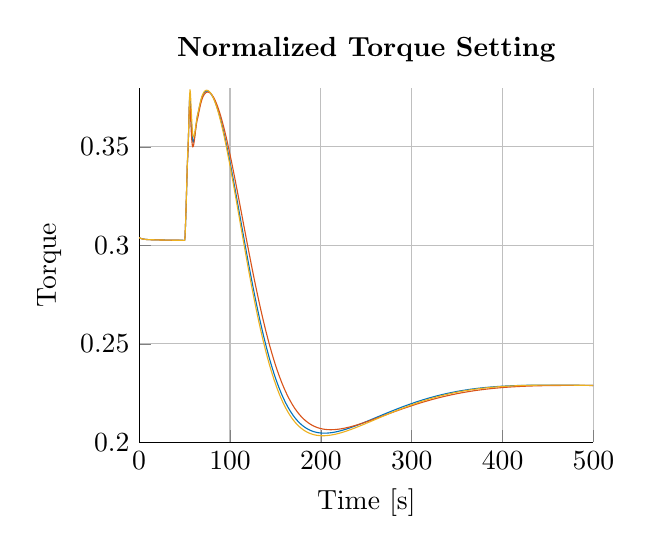
\begin{tikzpicture}

\begin{axis}[%
width=5.77cm,
height=4.5cm,
at={(0cm,0cm)},
scale only axis,
xmin=0,
xmax=500,
xlabel={Time [s]},
xmajorgrids,
ymin=0.2,
ymax=0.38,
ylabel={Torque},
ymajorgrids,
axis background/.style={fill=white},
title style={font=\bfseries},
title={Normalized Torque Setting},
axis x line*=bottom,
axis y line*=left
]
\addplot [color=mycolor1,solid,forget plot]
  table[row sep=crcr]{%
0	0.3039573152\\
0.5	0.303775988\\
1	0.303680777\\
1.5	0.303591625\\
2	0.303511058\\
2.5	0.303437863\\
3	0.303371714\\
3.5	0.303312209\\
4	0.303258903\\
4.5	0.30321133\\
5	0.303169016\\
5.5	0.303131484\\
6	0.30309827\\
6.5	0.303068925\\
7	0.303043022\\
7.5	0.30302016\\
8	0.30299996\\
8.5	0.30298209\\
9	0.30296622\\
9.5	0.30295207\\
10	0.30293939\\
10.5	0.30292794\\
11	0.30291752\\
11.5	0.30290797\\
12	0.30289911\\
12.5	0.30289083\\
13	0.302883\\
13.5	0.30287554\\
14	0.30286837\\
14.5	0.30286141\\
15	0.30285462\\
15.5	0.30284795\\
16	0.30284137\\
16.5	0.30283486\\
17	0.3028284\\
17.5	0.30282197\\
18	0.30281558\\
18.5	0.30280921\\
19	0.30280286\\
19.5	0.30279654\\
20	0.30279025\\
20.5	0.302784\\
21	0.30277779\\
21.5	0.30277162\\
22	0.30276551\\
22.5	0.30275946\\
23	0.30275348\\
23.5	0.30274757\\
24	0.30274173\\
24.5	0.30273598\\
25	0.30273032\\
25.5	0.30272476\\
26	0.30271928\\
26.5	0.30271391\\
27	0.30270864\\
27.5	0.30270347\\
28	0.30269841\\
28.5	0.30269345\\
29	0.3026886\\
29.5	0.30268385\\
30	0.30267921\\
30.5	0.30267467\\
31	0.30267023\\
31.5	0.3026659\\
32	0.30266167\\
32.5	0.30265754\\
33	0.30265351\\
33.5	0.30264957\\
34	0.30264573\\
34.5	0.30264198\\
35	0.30263832\\
35.5	0.30263475\\
36	0.30263126\\
36.5	0.30262786\\
37	0.30262454\\
37.5	0.3026213\\
38	0.30261814\\
38.5	0.30261505\\
39	0.30261204\\
39.5	0.3026091\\
40	0.30260623\\
40.5	0.30260343\\
41	0.30260069\\
41.5	0.30259802\\
42	0.30259541\\
42.5	0.30259287\\
43	0.30259038\\
43.5	0.30258795\\
44	0.30258558\\
44.5	0.30258327\\
45	0.30258101\\
45.5	0.3025788\\
46	0.30257665\\
46.5	0.30257454\\
47	0.30257249\\
47.5	0.30257048\\
48	0.30256852\\
48.5	0.3025666\\
49	0.30256473\\
49.5	0.30256291\\
50	0.30256112\\
50.5	0.304394478\\
51	0.31005118\\
51.5	0.3167577\\
52	0.3244155\\
52.5	0.332599\\
53	0.3409423\\
53.5	0.3457664\\
54	0.3514671\\
54.5	0.3592328\\
55	0.3680617\\
55.5	0.3746969\\
56	0.3750856\\
56.5	0.371095\\
57	0.3662848\\
57.5	0.3615689\\
58	0.3575059\\
58.5	0.3545839\\
59	0.3529578\\
59.5	0.3524559\\
60	0.3528279\\
60.5	0.3538361\\
61	0.3552738\\
61.5	0.356968\\
62	0.358779\\
62.5	0.360597\\
63	0.3623409\\
63.5	0.3639582\\
64	0.3654233\\
64.5	0.3665418\\
65	0.3674821\\
65.5	0.3685874\\
66	0.3696727\\
66.5	0.3707071\\
67	0.3717085\\
67.5	0.3726746\\
68	0.3735685\\
68.5	0.374377\\
69	0.3750961\\
69.5	0.3757275\\
70	0.3762754\\
70.5	0.3767459\\
71	0.3771453\\
71.5	0.3774796\\
72	0.3777542\\
72.5	0.3779738\\
73	0.3781422\\
73.5	0.3782629\\
74	0.3783385\\
74.5	0.3783715\\
75	0.3783635\\
75.5	0.3783164\\
76	0.3782313\\
76.5	0.3781093\\
77	0.3779515\\
77.5	0.3777586\\
78	0.3775314\\
78.5	0.3772706\\
79	0.3769767\\
79.5	0.3766505\\
80	0.3762924\\
80.5	0.3759031\\
81	0.375483\\
81.5	0.3750327\\
82	0.3745528\\
82.5	0.3740438\\
83	0.3735062\\
83.5	0.3729406\\
84	0.3723476\\
84.5	0.3717277\\
85	0.3710814\\
85.5	0.3704093\\
86	0.3697121\\
86.5	0.3689901\\
87	0.3682441\\
87.5	0.3674746\\
88	0.366682\\
88.5	0.3658671\\
89	0.3650303\\
89.5	0.3641722\\
90	0.3632934\\
90.5	0.3623945\\
91	0.3614759\\
91.5	0.3605382\\
92	0.3595821\\
92.5	0.358608\\
93	0.3576164\\
93.5	0.356608\\
94	0.3555833\\
94.5	0.3545428\\
95	0.3534869\\
95.5	0.3524164\\
96	0.3513316\\
96.5	0.3502332\\
97	0.3491215\\
97.5	0.3479972\\
98	0.3468608\\
98.5	0.3457127\\
99	0.3445534\\
99.5	0.3433835\\
100	0.3422035\\
100.5	0.3410137\\
101	0.3398148\\
101.5	0.3386072\\
102	0.3373913\\
102.5	0.3361676\\
103	0.3349366\\
103.5	0.3336988\\
104	0.3324546\\
104.5	0.3312044\\
105	0.3299487\\
105.5	0.3286879\\
106	0.3274225\\
106.5	0.3261529\\
107	0.3248794\\
107.5	0.3236026\\
108	0.3223228\\
108.5	0.3210404\\
109	0.3197558\\
109.5	0.3184695\\
110	0.3171818\\
110.5	0.315893\\
111	0.3146036\\
111.5	0.31331389\\
112	0.31202429\\
112.5	0.31073512\\
113	0.30944674\\
113.5	0.30815949\\
114	0.30687372\\
114.5	0.30558974\\
115	0.304307896\\
115.5	0.303028495\\
116	0.30175185\\
116.5	0.30047828\\
117	0.29920807\\
117.5	0.29794152\\
118	0.29667892\\
118.5	0.29542055\\
119	0.29416668\\
119.5	0.2929176\\
120	0.2916735\\
120.5	0.2904348\\
121	0.2892016\\
121.5	0.2879742\\
122	0.2867528\\
122.5	0.2855377\\
123	0.284329\\
123.5	0.2831271\\
124	0.2819321\\
124.5	0.2807442\\
125	0.2795636\\
125.5	0.2783906\\
126	0.2772252\\
126.5	0.2760678\\
127	0.2749184\\
127.5	0.2737773\\
128	0.2726445\\
128.5	0.2715204\\
129	0.2704049\\
129.5	0.2692983\\
130	0.2682008\\
130.5	0.2671123\\
131	0.2660331\\
131.5	0.2649633\\
132	0.2639031\\
132.5	0.2628524\\
133	0.2618115\\
133.5	0.2607804\\
134	0.2597593\\
134.5	0.2587481\\
135	0.2577471\\
135.5	0.2567562\\
136	0.2557756\\
136.5	0.2548054\\
137	0.2538455\\
137.5	0.2528961\\
138	0.2519572\\
138.5	0.2510288\\
139	0.2501111\\
139.5	0.249204\\
140	0.2483075\\
140.5	0.2474218\\
141	0.2465469\\
141.5	0.2456826\\
142	0.2448292\\
142.5	0.2439866\\
143	0.2431547\\
143.5	0.2423337\\
144	0.2415235\\
144.5	0.2407241\\
145	0.2399355\\
145.5	0.2391576\\
146	0.2383906\\
146.5	0.2376343\\
147	0.2368888\\
147.5	0.236154\\
148	0.2354298\\
148.5	0.2347164\\
149	0.2340135\\
149.5	0.2333212\\
150	0.2326395\\
150.5	0.2319683\\
151	0.2313076\\
151.5	0.2306572\\
152	0.2300172\\
152.5	0.2293876\\
153	0.2287682\\
153.5	0.2281589\\
154	0.2275598\\
154.5	0.2269708\\
155	0.2263918\\
155.5	0.2258227\\
156	0.2252635\\
156.5	0.2247141\\
157	0.2241744\\
157.5	0.2236444\\
158	0.2231239\\
158.5	0.222613\\
159	0.2221114\\
159.5	0.2216193\\
160	0.2211363\\
160.5	0.2206626\\
161	0.2201979\\
161.5	0.2197423\\
162	0.2192955\\
162.5	0.2188577\\
163	0.2184285\\
163.5	0.218008\\
164	0.2175961\\
164.5	0.2171927\\
165	0.2167977\\
165.5	0.2164109\\
166	0.2160324\\
166.5	0.215662\\
167	0.2152996\\
167.5	0.2149451\\
168	0.2145985\\
168.5	0.2142597\\
169	0.2139284\\
169.5	0.2136048\\
170	0.2132886\\
170.5	0.2129798\\
171	0.2126782\\
171.5	0.2123839\\
172	0.2120966\\
172.5	0.2118163\\
173	0.211543\\
173.5	0.2112764\\
174	0.2110166\\
174.5	0.2107634\\
175	0.2105168\\
175.5	0.2102766\\
176	0.2100427\\
176.5	0.2098152\\
177	0.2095938\\
177.5	0.2093784\\
178	0.2091691\\
178.5	0.2089657\\
179	0.2087682\\
179.5	0.2085763\\
180	0.2083902\\
180.5	0.2082095\\
181	0.2080344\\
181.5	0.2078647\\
182	0.2077003\\
182.5	0.2075411\\
183	0.207387\\
183.5	0.2072381\\
184	0.2070941\\
184.5	0.206955\\
185	0.2068208\\
185.5	0.2066913\\
186	0.2065664\\
186.5	0.2064462\\
187	0.2063305\\
187.5	0.2062193\\
188	0.2061124\\
188.5	0.2060098\\
189	0.2059114\\
189.5	0.2058172\\
190	0.2057271\\
190.5	0.205641\\
191	0.2055589\\
191.5	0.2054806\\
192	0.2054062\\
192.5	0.2053354\\
193	0.2052684\\
193.5	0.205205\\
194	0.2051451\\
194.5	0.2050888\\
195	0.2050358\\
195.5	0.2049863\\
196	0.20494\\
196.5	0.204897\\
197	0.2048571\\
197.5	0.2048204\\
198	0.2047868\\
198.5	0.2047562\\
199	0.2047285\\
199.5	0.2047038\\
200	0.2046819\\
200.5	0.2046628\\
201	0.2046464\\
201.5	0.2046328\\
202	0.2046218\\
202.5	0.2046134\\
203	0.2046075\\
203.5	0.2046042\\
204	0.2046033\\
204.5	0.2046048\\
205	0.2046086\\
205.5	0.2046148\\
206	0.2046232\\
206.5	0.2046339\\
207	0.2046467\\
207.5	0.2046617\\
208	0.2046788\\
208.5	0.2046979\\
209	0.204719\\
209.5	0.2047422\\
210	0.2047672\\
210.5	0.2047942\\
211	0.204823\\
211.5	0.2048536\\
212	0.204886\\
212.5	0.2049201\\
213	0.204956\\
213.5	0.2049935\\
214	0.2050327\\
214.5	0.2050735\\
215	0.2051159\\
215.5	0.2051598\\
216	0.2052052\\
216.5	0.2052521\\
217	0.2053004\\
217.5	0.2053502\\
218	0.2054013\\
218.5	0.2054538\\
219	0.2055076\\
219.5	0.2055627\\
220	0.2056191\\
220.5	0.2056767\\
221	0.2057356\\
221.5	0.2057956\\
222	0.2058568\\
222.5	0.2059191\\
223	0.2059825\\
223.5	0.206047\\
224	0.2061126\\
224.5	0.2061792\\
225	0.2062468\\
225.5	0.2063154\\
226	0.2063849\\
226.5	0.2064554\\
227	0.2065268\\
227.5	0.2065991\\
228	0.2066723\\
228.5	0.2067463\\
229	0.2068212\\
229.5	0.2068969\\
230	0.2069734\\
230.5	0.2070506\\
231	0.2071286\\
231.5	0.2072073\\
232	0.2072867\\
232.5	0.2073669\\
233	0.2074477\\
233.5	0.2075291\\
234	0.2076112\\
234.5	0.2076939\\
235	0.2077773\\
235.5	0.2078612\\
236	0.2079456\\
236.5	0.2080307\\
237	0.2081163\\
237.5	0.2082024\\
238	0.208289\\
238.5	0.2083761\\
239	0.2084636\\
239.5	0.2085517\\
240	0.2086401\\
240.5	0.2087291\\
241	0.2088184\\
241.5	0.2089081\\
242	0.2089982\\
242.5	0.2090888\\
243	0.2091796\\
243.5	0.2092708\\
244	0.2093624\\
244.5	0.2094543\\
245	0.2095465\\
245.5	0.209639\\
246	0.2097317\\
246.5	0.2098248\\
247	0.2099181\\
247.5	0.2100117\\
248	0.2101055\\
248.5	0.2101995\\
249	0.2102938\\
249.5	0.2103883\\
250	0.2104829\\
};
\addplot [color=mycolor1,solid,forget plot]
  table[row sep=crcr]{%
250	0.2104829\\
250.5	0.2105778\\
251	0.2106728\\
251.5	0.210768\\
252	0.2108634\\
252.5	0.2109589\\
253	0.2110545\\
253.5	0.2111503\\
254	0.2112462\\
254.5	0.2113422\\
255	0.2114383\\
255.5	0.2115344\\
256	0.2116307\\
256.5	0.211727\\
257	0.2118234\\
257.5	0.2119199\\
258	0.2120164\\
258.5	0.2121129\\
259	0.2122095\\
259.5	0.2123061\\
260	0.2124027\\
260.5	0.2124993\\
261	0.212596\\
261.5	0.2126926\\
262	0.2127892\\
262.5	0.2128857\\
263	0.2129823\\
263.5	0.2130788\\
264	0.2131752\\
264.5	0.2132716\\
265	0.213368\\
265.5	0.2134643\\
266	0.2135605\\
266.5	0.2136566\\
267	0.2137527\\
267.5	0.2138487\\
268	0.2139445\\
268.5	0.2140403\\
269	0.2141359\\
269.5	0.2142315\\
270	0.2143269\\
270.5	0.2144222\\
271	0.2145174\\
271.5	0.2146124\\
272	0.2147073\\
272.5	0.214802\\
273	0.2148966\\
273.5	0.2149911\\
274	0.2150853\\
274.5	0.2151794\\
275	0.2152734\\
275.5	0.2153671\\
276	0.2154607\\
276.5	0.215554\\
277	0.2156472\\
277.5	0.2157402\\
278	0.215833\\
278.5	0.2159256\\
279	0.2160179\\
279.5	0.2161101\\
280	0.216202\\
280.5	0.2162937\\
281	0.2163852\\
281.5	0.2164765\\
282	0.2165675\\
282.5	0.2166583\\
283	0.2167488\\
283.5	0.2168391\\
284	0.2169291\\
284.5	0.2170189\\
285	0.2171084\\
285.5	0.2171977\\
286	0.2172867\\
286.5	0.2173754\\
287	0.2174639\\
287.5	0.2175521\\
288	0.21764\\
288.5	0.2177276\\
289	0.2178149\\
289.5	0.217902\\
290	0.2179887\\
290.5	0.2180752\\
291	0.2181614\\
291.5	0.2182472\\
292	0.2183328\\
292.5	0.2184181\\
293	0.218503\\
293.5	0.2185877\\
294	0.218672\\
294.5	0.218756\\
295	0.2188397\\
295.5	0.2189231\\
296	0.2190061\\
296.5	0.2190889\\
297	0.2191713\\
297.5	0.2192534\\
298	0.2193351\\
298.5	0.2194165\\
299	0.2194976\\
299.5	0.2195783\\
300	0.2196587\\
300.5	0.2197387\\
301	0.2198184\\
301.5	0.2198978\\
302	0.2199768\\
302.5	0.2200555\\
303	0.2201338\\
303.5	0.2202117\\
304	0.2202893\\
304.5	0.2203666\\
305	0.2204435\\
305.5	0.22052\\
306	0.2205962\\
306.5	0.220672\\
307	0.2207474\\
307.5	0.2208225\\
308	0.2208972\\
308.5	0.2209715\\
309	0.2210455\\
309.5	0.2211191\\
310	0.2211923\\
310.5	0.2212652\\
311	0.2213377\\
311.5	0.2214098\\
312	0.2214815\\
312.5	0.2215529\\
313	0.2216238\\
313.5	0.2216944\\
314	0.2217647\\
314.5	0.2218345\\
315	0.221904\\
315.5	0.221973\\
316	0.2220417\\
316.5	0.22211\\
317	0.222178\\
317.5	0.2222455\\
318	0.2223127\\
318.5	0.2223794\\
319	0.2224458\\
319.5	0.2225118\\
320	0.2225774\\
320.5	0.2226426\\
321	0.2227075\\
321.5	0.2227719\\
322	0.222836\\
322.5	0.2228996\\
323	0.2229629\\
323.5	0.2230258\\
324	0.2230883\\
324.5	0.2231504\\
325	0.2232121\\
325.5	0.2232735\\
326	0.2233344\\
326.5	0.2233949\\
327	0.2234551\\
327.5	0.2235149\\
328	0.2235742\\
328.5	0.2236332\\
329	0.2236918\\
329.5	0.22375\\
330	0.2238078\\
330.5	0.2238653\\
331	0.2239223\\
331.5	0.2239789\\
332	0.2240352\\
332.5	0.2240911\\
333	0.2241465\\
333.5	0.2242016\\
334	0.2242563\\
334.5	0.2243106\\
335	0.2243646\\
335.5	0.2244181\\
336	0.2244713\\
336.5	0.224524\\
337	0.2245764\\
337.5	0.2246284\\
338	0.22468\\
338.5	0.2247313\\
339	0.2247821\\
339.5	0.2248326\\
340	0.2248827\\
340.5	0.2249324\\
341	0.2249817\\
341.5	0.2250306\\
342	0.2250792\\
342.5	0.2251274\\
343	0.2251752\\
343.5	0.2252226\\
344	0.2252697\\
344.5	0.2253164\\
345	0.2253627\\
345.5	0.2254086\\
346	0.2254542\\
346.5	0.2254993\\
347	0.2255442\\
347.5	0.2255886\\
348	0.2256327\\
348.5	0.2256764\\
349	0.2257198\\
349.5	0.2257627\\
350	0.2258053\\
350.5	0.2258476\\
351	0.2258895\\
351.5	0.225931\\
352	0.2259722\\
352.5	0.226013\\
353	0.2260534\\
353.5	0.2260935\\
354	0.2261333\\
354.5	0.2261727\\
355	0.2262117\\
355.5	0.2262504\\
356	0.2262887\\
356.5	0.2263267\\
357	0.2263643\\
357.5	0.2264016\\
358	0.2264385\\
358.5	0.2264751\\
359	0.2265114\\
359.5	0.2265473\\
360	0.2265828\\
360.5	0.2266181\\
361	0.2266529\\
361.5	0.2266875\\
362	0.2267217\\
362.5	0.2267556\\
363	0.2267892\\
363.5	0.2268224\\
364	0.2268553\\
364.5	0.2268878\\
365	0.2269201\\
365.5	0.226952\\
366	0.2269836\\
366.5	0.2270148\\
367	0.2270458\\
367.5	0.2270764\\
368	0.2271067\\
368.5	0.2271367\\
369	0.2271664\\
369.5	0.2271958\\
370	0.2272248\\
370.5	0.2272536\\
371	0.227282\\
371.5	0.2273101\\
372	0.2273379\\
372.5	0.2273655\\
373	0.2273927\\
373.5	0.2274196\\
374	0.2274462\\
374.5	0.2274726\\
375	0.2274986\\
375.5	0.2275243\\
376	0.2275498\\
376.5	0.2275749\\
377	0.2275998\\
377.5	0.2276244\\
378	0.2276486\\
378.5	0.2276726\\
379	0.2276964\\
379.5	0.2277198\\
380	0.227743\\
380.5	0.2277659\\
381	0.2277885\\
381.5	0.2278108\\
382	0.2278329\\
382.5	0.2278547\\
383	0.2278762\\
383.5	0.2278975\\
384	0.2279185\\
384.5	0.2279392\\
385	0.2279597\\
385.5	0.2279799\\
386	0.2279998\\
386.5	0.2280195\\
387	0.2280389\\
387.5	0.2280581\\
388	0.2280771\\
388.5	0.2280957\\
389	0.2281142\\
389.5	0.2281324\\
390	0.2281503\\
390.5	0.228168\\
391	0.2281855\\
391.5	0.2282027\\
392	0.2282197\\
392.5	0.2282364\\
393	0.2282529\\
393.5	0.2282692\\
394	0.2282852\\
394.5	0.2283011\\
395	0.2283166\\
395.5	0.228332\\
396	0.2283471\\
396.5	0.2283621\\
397	0.2283768\\
397.5	0.2283912\\
398	0.2284055\\
398.5	0.2284195\\
399	0.2284334\\
399.5	0.228447\\
400	0.2284604\\
400.5	0.2284736\\
401	0.2284866\\
401.5	0.2284994\\
402	0.228512\\
402.5	0.2285243\\
403	0.2285365\\
403.5	0.2285485\\
404	0.2285603\\
404.5	0.2285719\\
405	0.2285833\\
405.5	0.2285945\\
406	0.2286055\\
406.5	0.2286163\\
407	0.228627\\
407.5	0.2286374\\
408	0.2286477\\
408.5	0.2286578\\
409	0.2286677\\
409.5	0.2286774\\
410	0.228687\\
410.5	0.2286963\\
411	0.2287055\\
411.5	0.2287146\\
412	0.2287234\\
412.5	0.2287321\\
413	0.2287407\\
413.5	0.228749\\
414	0.2287572\\
414.5	0.2287652\\
415	0.2287731\\
415.5	0.2287808\\
416	0.2287884\\
416.5	0.2287958\\
417	0.228803\\
417.5	0.2288101\\
418	0.228817\\
418.5	0.2288238\\
419	0.2288305\\
419.5	0.228837\\
420	0.2288433\\
420.5	0.2288495\\
421	0.2288556\\
421.5	0.2288615\\
422	0.2288673\\
422.5	0.2288729\\
423	0.2288784\\
423.5	0.2288838\\
424	0.228889\\
424.5	0.2288941\\
425	0.2288991\\
425.5	0.228904\\
426	0.2289087\\
426.5	0.2289133\\
427	0.2289177\\
427.5	0.2289221\\
428	0.2289263\\
428.5	0.2289304\\
429	0.2289344\\
429.5	0.2289382\\
430	0.228942\\
430.5	0.2289456\\
431	0.2289491\\
431.5	0.2289525\\
432	0.2289558\\
432.5	0.228959\\
433	0.2289621\\
433.5	0.2289651\\
434	0.2289679\\
434.5	0.2289707\\
435	0.2289733\\
435.5	0.2289759\\
436	0.2289783\\
436.5	0.2289807\\
437	0.228983\\
437.5	0.2289851\\
438	0.2289872\\
438.5	0.2289892\\
439	0.228991\\
439.5	0.2289928\\
440	0.2289945\\
440.5	0.2289961\\
441	0.2289976\\
441.5	0.2289991\\
442	0.2290004\\
442.5	0.2290017\\
443	0.2290029\\
443.5	0.2290039\\
444	0.229005\\
444.5	0.2290059\\
445	0.2290068\\
445.5	0.2290075\\
446	0.2290082\\
446.5	0.2290089\\
447	0.2290094\\
447.5	0.2290099\\
448	0.2290103\\
448.5	0.2290106\\
449	0.2290109\\
449.5	0.2290111\\
450	0.2290112\\
450.5	0.2290113\\
451	0.2290113\\
451.5	0.2290112\\
452	0.2290111\\
452.5	0.2290109\\
453	0.2290106\\
453.5	0.2290103\\
454	0.22901\\
454.5	0.2290095\\
455	0.229009\\
455.5	0.2290085\\
456	0.2290079\\
456.5	0.2290072\\
457	0.2290065\\
457.5	0.2290057\\
458	0.2290049\\
458.5	0.2290041\\
459	0.2290031\\
459.5	0.2290022\\
460	0.2290012\\
460.5	0.2290001\\
461	0.228999\\
461.5	0.2289978\\
462	0.2289966\\
462.5	0.2289954\\
463	0.2289941\\
463.5	0.2289928\\
464	0.2289914\\
464.5	0.22899\\
465	0.2289885\\
465.5	0.2289871\\
466	0.2289855\\
466.5	0.228984\\
467	0.2289824\\
467.5	0.2289807\\
468	0.228979\\
468.5	0.2289773\\
469	0.2289756\\
469.5	0.2289738\\
470	0.228972\\
470.5	0.2289702\\
471	0.2289683\\
471.5	0.2289664\\
472	0.2289645\\
472.5	0.2289625\\
473	0.2289605\\
473.5	0.2289585\\
474	0.2289565\\
474.5	0.2289544\\
475	0.2289523\\
475.5	0.2289502\\
476	0.2289481\\
476.5	0.2289459\\
477	0.2289437\\
477.5	0.2289415\\
478	0.2289393\\
478.5	0.2289371\\
479	0.2289348\\
479.5	0.2289325\\
480	0.2289302\\
480.5	0.2289279\\
481	0.2289255\\
481.5	0.2289232\\
482	0.2289208\\
482.5	0.2289184\\
483	0.228916\\
483.5	0.2289136\\
484	0.2289111\\
484.5	0.2289087\\
485	0.2289062\\
485.5	0.2289038\\
486	0.2289013\\
486.5	0.2288988\\
487	0.2288962\\
487.5	0.2288937\\
488	0.2288912\\
488.5	0.2288886\\
489	0.2288861\\
489.5	0.2288835\\
490	0.228881\\
490.5	0.2288784\\
491	0.2288758\\
491.5	0.2288732\\
492	0.2288706\\
492.5	0.228868\\
493	0.2288654\\
493.5	0.2288628\\
494	0.2288601\\
494.5	0.2288575\\
495	0.2288549\\
495.5	0.2288522\\
496	0.2288496\\
496.5	0.2288469\\
497	0.2288443\\
497.5	0.2288416\\
498	0.228839\\
498.5	0.2288363\\
499	0.2288337\\
499.5	0.228831\\
};
\addplot [color=mycolor2,solid,forget plot]
  table[row sep=crcr]{%
0	0.3039552245\\
0.5	0.303765592\\
1	0.303666922\\
1.5	0.303574787\\
2	0.30349186\\
2.5	0.30341683\\
3	0.303349327\\
3.5	0.303288902\\
4	0.303235058\\
4.5	0.303187277\\
5	0.303145034\\
5.5	0.303107805\\
6	0.303075079\\
6.5	0.303046365\\
7	0.303021198\\
7.5	0.30299914\\
8	0.30297979\\
8.5	0.30296278\\
9	0.30294777\\
9.5	0.30293446\\
10	0.30292257\\
10.5	0.30291187\\
11	0.30290214\\
11.5	0.30289321\\
12	0.30288491\\
12.5	0.30287712\\
13	0.30286972\\
13.5	0.30286262\\
14	0.30285574\\
14.5	0.30284902\\
15	0.30284241\\
15.5	0.30283587\\
16	0.30282937\\
16.5	0.3028229\\
17	0.30281644\\
17.5	0.30280998\\
18	0.30280353\\
18.5	0.30279707\\
19	0.30279063\\
19.5	0.30278419\\
20	0.30277777\\
20.5	0.30277137\\
21	0.30276501\\
21.5	0.30275869\\
22	0.30275243\\
22.5	0.30274622\\
23	0.30274008\\
23.5	0.30273401\\
24	0.30272803\\
24.5	0.30272213\\
25	0.30271633\\
25.5	0.30271062\\
26	0.30270501\\
26.5	0.30269951\\
27	0.30269412\\
27.5	0.30268883\\
28	0.30268365\\
28.5	0.30267859\\
29	0.30267363\\
29.5	0.30266878\\
30	0.30266404\\
30.5	0.30265942\\
31	0.30265489\\
31.5	0.30265048\\
32	0.30264617\\
32.5	0.30264196\\
33	0.30263785\\
33.5	0.30263384\\
34	0.30262992\\
34.5	0.3026261\\
35	0.30262237\\
35.5	0.30261874\\
36	0.30261518\\
36.5	0.30261172\\
37	0.30260833\\
37.5	0.30260503\\
38	0.30260181\\
38.5	0.30259866\\
39	0.30259559\\
39.5	0.30259259\\
40	0.30258966\\
40.5	0.3025868\\
41	0.30258401\\
41.5	0.30258128\\
42	0.30257862\\
42.5	0.30257601\\
43	0.30257347\\
43.5	0.30257099\\
44	0.30256857\\
44.5	0.3025662\\
45	0.30256389\\
45.5	0.30256163\\
46	0.30255943\\
46.5	0.30255727\\
47	0.30255516\\
47.5	0.30255311\\
48	0.3025511\\
48.5	0.30254913\\
49	0.30254722\\
49.5	0.30254534\\
50	0.30254351\\
50.5	0.304471449\\
51	0.31042517\\
51.5	0.3174263\\
52	0.325291\\
52.5	0.3334964\\
53	0.3408456\\
53.5	0.3451152\\
54	0.3508922\\
54.5	0.3592195\\
55	0.3683954\\
55.5	0.3736534\\
56	0.3715522\\
56.5	0.3663626\\
57	0.3610624\\
57.5	0.356449\\
58	0.3529859\\
58.5	0.3509046\\
59	0.3500809\\
59.5	0.3502514\\
60	0.3511626\\
60.5	0.3525872\\
61	0.3543252\\
61.5	0.3562077\\
62	0.3580983\\
62.5	0.3598939\\
63	0.3615241\\
63.5	0.3629525\\
64	0.3640551\\
64.5	0.3647738\\
65	0.3659146\\
65.5	0.3671063\\
66	0.3682674\\
66.5	0.3693898\\
67	0.3704737\\
67.5	0.3714837\\
68	0.3724073\\
68.5	0.3732412\\
69	0.3739872\\
69.5	0.3746488\\
70	0.3752313\\
70.5	0.375741\\
71	0.3761835\\
71.5	0.3765645\\
72	0.3768889\\
72.5	0.3771609\\
73	0.3773843\\
73.5	0.3775621\\
74	0.3776969\\
74.5	0.3777909\\
75	0.3778458\\
75.5	0.3778632\\
76	0.3778442\\
76.5	0.37779\\
77	0.3777015\\
77.5	0.3775793\\
78	0.3774244\\
78.5	0.3772372\\
79	0.3770184\\
79.5	0.3767686\\
80	0.3764883\\
80.5	0.376178\\
81	0.3758383\\
81.5	0.3754696\\
82	0.3750724\\
82.5	0.3746474\\
83	0.3741949\\
83.5	0.3737155\\
84	0.3732096\\
84.5	0.3726779\\
85	0.3721207\\
85.5	0.3715386\\
86	0.3709322\\
86.5	0.3703018\\
87	0.3696481\\
87.5	0.3689715\\
88	0.3682725\\
88.5	0.3675517\\
89	0.3668096\\
89.5	0.3660466\\
90	0.3652632\\
90.5	0.36446\\
91	0.3636375\\
91.5	0.3627962\\
92	0.3619365\\
92.5	0.361059\\
93	0.3601641\\
93.5	0.3592523\\
94	0.3583242\\
94.5	0.3573802\\
95	0.3564208\\
95.5	0.3554464\\
96	0.3544576\\
96.5	0.3534548\\
97	0.3524385\\
97.5	0.3514092\\
98	0.3503673\\
98.5	0.3493133\\
99	0.3482476\\
99.5	0.3471707\\
100	0.346083\\
100.5	0.344985\\
101	0.3438772\\
101.5	0.3427599\\
102	0.3416336\\
102.5	0.3404987\\
103	0.3393557\\
103.5	0.3382049\\
104	0.3370469\\
104.5	0.3358819\\
105	0.3347104\\
105.5	0.3335328\\
106	0.3323496\\
106.5	0.331161\\
107	0.3299675\\
107.5	0.3287695\\
108	0.3275673\\
108.5	0.3263614\\
109	0.325152\\
109.5	0.3239397\\
110	0.3227246\\
110.5	0.3215072\\
111	0.3202879\\
111.5	0.3190669\\
112	0.3178446\\
112.5	0.3166214\\
113	0.3153975\\
113.5	0.3141734\\
114	0.31294924\\
114.5	0.31172545\\
115	0.31050231\\
115.5	0.30928011\\
116	0.30805916\\
116.5	0.30683976\\
117	0.30562219\\
117.5	0.304406727\\
118	0.30319366\\
118.5	0.30198326\\
119	0.30077579\\
119.5	0.29957151\\
120	0.29837068\\
120.5	0.29717356\\
121	0.29598038\\
121.5	0.29479139\\
122	0.2936068\\
122.5	0.2924269\\
123	0.2912519\\
123.5	0.2900819\\
124	0.2889173\\
124.5	0.2877582\\
125	0.2866048\\
125.5	0.2854573\\
126	0.284316\\
126.5	0.2831809\\
127	0.2820524\\
127.5	0.2809304\\
128	0.2798154\\
128.5	0.2787073\\
129	0.2776064\\
129.5	0.2765128\\
130	0.2754266\\
130.5	0.2743481\\
131	0.2732773\\
131.5	0.2722144\\
132	0.2711596\\
132.5	0.2701129\\
133	0.2690744\\
133.5	0.2680443\\
134	0.2670228\\
134.5	0.2660098\\
135	0.2650055\\
135.5	0.2640101\\
136	0.2630235\\
136.5	0.2620459\\
137	0.2610774\\
137.5	0.260118\\
138	0.2591678\\
138.5	0.258227\\
139	0.2572954\\
139.5	0.2563733\\
140	0.2554607\\
140.5	0.2545575\\
141	0.253664\\
141.5	0.25278\\
142	0.2519057\\
142.5	0.2510411\\
143	0.2501863\\
143.5	0.2493411\\
144	0.2485058\\
144.5	0.2476802\\
145	0.2468645\\
145.5	0.2460586\\
146	0.2452625\\
146.5	0.2444762\\
147	0.2436998\\
147.5	0.2429333\\
148	0.2421766\\
148.5	0.2414297\\
149	0.2406926\\
149.5	0.2399654\\
150	0.239248\\
150.5	0.2385403\\
151	0.2378424\\
151.5	0.2371542\\
152	0.2364757\\
152.5	0.2358069\\
153	0.2351477\\
153.5	0.2344981\\
154	0.2338581\\
154.5	0.2332276\\
155	0.2326066\\
155.5	0.2319951\\
156	0.2313929\\
156.5	0.2308001\\
157	0.2302165\\
157.5	0.2296422\\
158	0.2290771\\
158.5	0.2285211\\
159	0.2279742\\
159.5	0.2274363\\
160	0.2269074\\
160.5	0.2263873\\
161	0.2258761\\
161.5	0.2253736\\
162	0.2248798\\
162.5	0.2243947\\
163	0.223918\\
163.5	0.2234499\\
164	0.2229902\\
164.5	0.2225388\\
165	0.2220956\\
165.5	0.2216607\\
166	0.2212339\\
166.5	0.2208151\\
167	0.2204042\\
167.5	0.2200013\\
168	0.2196061\\
168.5	0.2192187\\
169	0.2188389\\
169.5	0.2184667\\
170	0.218102\\
170.5	0.2177446\\
171	0.2173946\\
171.5	0.2170519\\
172	0.2167162\\
172.5	0.2163877\\
173	0.2160662\\
173.5	0.2157516\\
174	0.2154438\\
174.5	0.2151427\\
175	0.2148484\\
175.5	0.2145606\\
176	0.2142793\\
176.5	0.2140045\\
177	0.213736\\
177.5	0.2134737\\
178	0.2132177\\
178.5	0.2129677\\
179	0.2127237\\
179.5	0.2124857\\
180	0.2122536\\
180.5	0.2120272\\
181	0.2118065\\
181.5	0.2115914\\
182	0.2113819\\
182.5	0.2111779\\
183	0.2109792\\
183.5	0.2107859\\
184	0.2105978\\
184.5	0.2104148\\
185	0.2102369\\
185.5	0.210064\\
186	0.2098961\\
186.5	0.209733\\
187	0.2095748\\
187.5	0.2094212\\
188	0.2092723\\
188.5	0.2091279\\
189	0.2089881\\
189.5	0.2088527\\
190	0.2087216\\
190.5	0.2085949\\
191	0.2084723\\
191.5	0.208354\\
192	0.2082397\\
192.5	0.2081295\\
193	0.2080232\\
193.5	0.2079208\\
194	0.2078223\\
194.5	0.2077275\\
195	0.2076365\\
195.5	0.2075491\\
196	0.2074653\\
196.5	0.207385\\
197	0.2073082\\
197.5	0.2072349\\
198	0.2071648\\
198.5	0.2070981\\
199	0.2070346\\
199.5	0.2069743\\
200	0.2069172\\
200.5	0.2068631\\
201	0.2068121\\
201.5	0.206764\\
202	0.2067188\\
202.5	0.2066766\\
203	0.2066371\\
203.5	0.2066004\\
204	0.2065664\\
204.5	0.2065352\\
205	0.2065065\\
205.5	0.2064804\\
206	0.2064569\\
206.5	0.2064358\\
207	0.2064172\\
207.5	0.2064009\\
208	0.2063871\\
208.5	0.2063755\\
209	0.2063662\\
209.5	0.2063591\\
210	0.2063543\\
210.5	0.2063515\\
211	0.2063509\\
211.5	0.2063523\\
212	0.2063558\\
212.5	0.2063612\\
213	0.2063686\\
213.5	0.2063779\\
214	0.2063891\\
214.5	0.2064022\\
215	0.206417\\
215.5	0.2064336\\
216	0.206452\\
216.5	0.206472\\
217	0.2064937\\
217.5	0.2065171\\
218	0.206542\\
218.5	0.2065686\\
219	0.2065967\\
219.5	0.2066263\\
220	0.2066573\\
220.5	0.2066898\\
221	0.2067238\\
221.5	0.2067591\\
222	0.2067958\\
222.5	0.2068339\\
223	0.2068732\\
223.5	0.2069139\\
224	0.2069558\\
224.5	0.2069989\\
225	0.2070432\\
225.5	0.2070887\\
226	0.2071354\\
226.5	0.2071832\\
227	0.2072321\\
227.5	0.2072821\\
228	0.2073331\\
228.5	0.2073852\\
229	0.2074383\\
229.5	0.2074924\\
230	0.2075474\\
230.5	0.2076034\\
231	0.2076603\\
231.5	0.2077182\\
232	0.2077769\\
232.5	0.2078365\\
233	0.2078969\\
233.5	0.2079582\\
234	0.2080202\\
234.5	0.2080831\\
235	0.2081467\\
235.5	0.2082111\\
236	0.2082762\\
236.5	0.208342\\
237	0.2084085\\
237.5	0.2084757\\
238	0.2085435\\
238.5	0.2086121\\
239	0.2086812\\
239.5	0.2087509\\
240	0.2088213\\
240.5	0.2088922\\
241	0.2089637\\
241.5	0.2090358\\
242	0.2091084\\
242.5	0.2091815\\
243	0.2092552\\
243.5	0.2093293\\
244	0.2094039\\
244.5	0.209479\\
245	0.2095545\\
245.5	0.2096305\\
246	0.2097069\\
246.5	0.2097837\\
247	0.2098609\\
247.5	0.2099385\\
248	0.2100165\\
248.5	0.2100948\\
249	0.2101735\\
249.5	0.2102526\\
250	0.210332\\
};
\addplot [color=mycolor2,solid,forget plot]
  table[row sep=crcr]{%
250	0.210332\\
250.5	0.2104117\\
251	0.2104917\\
251.5	0.210572\\
252	0.2106526\\
252.5	0.2107334\\
253	0.2108146\\
253.5	0.2108959\\
254	0.2109776\\
254.5	0.2110594\\
255	0.2111415\\
255.5	0.2112238\\
256	0.2113064\\
256.5	0.2113891\\
257	0.211472\\
257.5	0.211555\\
258	0.2116383\\
258.5	0.2117217\\
259	0.2118053\\
259.5	0.211889\\
260	0.2119728\\
260.5	0.2120568\\
261	0.2121408\\
261.5	0.212225\\
262	0.2123093\\
262.5	0.2123937\\
263	0.2124782\\
263.5	0.2125628\\
264	0.2126474\\
264.5	0.2127321\\
265	0.2128168\\
265.5	0.2129016\\
266	0.2129865\\
266.5	0.2130714\\
267	0.2131563\\
267.5	0.2132412\\
268	0.2133262\\
268.5	0.2134111\\
269	0.2134961\\
269.5	0.2135811\\
270	0.213666\\
270.5	0.213751\\
271	0.2138359\\
271.5	0.2139208\\
272	0.2140056\\
272.5	0.2140904\\
273	0.2141752\\
273.5	0.2142599\\
274	0.2143446\\
274.5	0.2144292\\
275	0.2145138\\
275.5	0.2145983\\
276	0.2146826\\
276.5	0.214767\\
277	0.2148512\\
277.5	0.2149353\\
278	0.2150194\\
278.5	0.2151033\\
279	0.2151872\\
279.5	0.2152709\\
280	0.2153545\\
280.5	0.215438\\
281	0.2155214\\
281.5	0.2156046\\
282	0.2156877\\
282.5	0.2157707\\
283	0.2158535\\
283.5	0.2159362\\
284	0.2160187\\
284.5	0.2161011\\
285	0.2161834\\
285.5	0.2162654\\
286	0.2163473\\
286.5	0.2164291\\
287	0.2165106\\
287.5	0.216592\\
288	0.2166732\\
288.5	0.2167543\\
289	0.2168351\\
289.5	0.2169158\\
290	0.2169962\\
290.5	0.2170765\\
291	0.2171566\\
291.5	0.2172364\\
292	0.2173161\\
292.5	0.2173955\\
293	0.2174748\\
293.5	0.2175538\\
294	0.2176326\\
294.5	0.2177112\\
295	0.2177896\\
295.5	0.2178677\\
296	0.2179456\\
296.5	0.2180233\\
297	0.2181008\\
297.5	0.218178\\
298	0.218255\\
298.5	0.2183317\\
299	0.2184082\\
299.5	0.2184845\\
300	0.2185605\\
300.5	0.2186362\\
301	0.2187117\\
301.5	0.218787\\
302	0.218862\\
302.5	0.2189367\\
303	0.2190112\\
303.5	0.2190854\\
304	0.2191593\\
304.5	0.219233\\
305	0.2193064\\
305.5	0.2193795\\
306	0.2194524\\
306.5	0.219525\\
307	0.2195973\\
307.5	0.2196693\\
308	0.2197411\\
308.5	0.2198126\\
309	0.2198838\\
309.5	0.2199547\\
310	0.2200253\\
310.5	0.2200956\\
311	0.2201657\\
311.5	0.2202354\\
312	0.2203049\\
312.5	0.2203741\\
313	0.220443\\
313.5	0.2205115\\
314	0.2205798\\
314.5	0.2206478\\
315	0.2207155\\
315.5	0.2207829\\
316	0.22085\\
316.5	0.2209168\\
317	0.2209833\\
317.5	0.2210494\\
318	0.2211153\\
318.5	0.2211809\\
319	0.2212461\\
319.5	0.2213111\\
320	0.2213757\\
320.5	0.2214401\\
321	0.2215041\\
321.5	0.2215678\\
322	0.2216312\\
322.5	0.2216943\\
323	0.221757\\
323.5	0.2218195\\
324	0.2218816\\
324.5	0.2219435\\
325	0.222005\\
325.5	0.2220661\\
326	0.222127\\
326.5	0.2221876\\
327	0.2222478\\
327.5	0.2223077\\
328	0.2223673\\
328.5	0.2224266\\
329	0.2224856\\
329.5	0.2225442\\
330	0.2226025\\
330.5	0.2226605\\
331	0.2227182\\
331.5	0.2227755\\
332	0.2228326\\
332.5	0.2228893\\
333	0.2229457\\
333.5	0.2230017\\
334	0.2230575\\
334.5	0.2231129\\
335	0.223168\\
335.5	0.2232227\\
336	0.2232772\\
336.5	0.2233313\\
337	0.2233851\\
337.5	0.2234386\\
338	0.2234917\\
338.5	0.2235446\\
339	0.2235971\\
339.5	0.2236493\\
340	0.2237011\\
340.5	0.2237527\\
341	0.2238039\\
341.5	0.2238548\\
342	0.2239054\\
342.5	0.2239556\\
343	0.2240056\\
343.5	0.2240552\\
344	0.2241045\\
344.5	0.2241535\\
345	0.2242021\\
345.5	0.2242504\\
346	0.2242984\\
346.5	0.2243461\\
347	0.2243935\\
347.5	0.2244406\\
348	0.2244873\\
348.5	0.2245337\\
349	0.2245798\\
349.5	0.2246256\\
350	0.2246711\\
350.5	0.2247162\\
351	0.2247611\\
351.5	0.2248056\\
352	0.2248498\\
352.5	0.2248937\\
353	0.2249373\\
353.5	0.2249806\\
354	0.2250235\\
354.5	0.2250662\\
355	0.2251085\\
355.5	0.2251506\\
356	0.2251923\\
356.5	0.2252337\\
357	0.2252748\\
357.5	0.2253156\\
358	0.2253561\\
358.5	0.2253963\\
359	0.2254362\\
359.5	0.2254757\\
360	0.225515\\
360.5	0.225554\\
361	0.2255927\\
361.5	0.225631\\
362	0.2256691\\
362.5	0.2257069\\
363	0.2257444\\
363.5	0.2257816\\
364	0.2258184\\
364.5	0.225855\\
365	0.2258913\\
365.5	0.2259273\\
366	0.225963\\
366.5	0.2259985\\
367	0.2260336\\
367.5	0.2260684\\
368	0.226103\\
368.5	0.2261372\\
369	0.2261712\\
369.5	0.2262049\\
370	0.2262383\\
370.5	0.2262714\\
371	0.2263043\\
371.5	0.2263368\\
372	0.2263691\\
372.5	0.2264011\\
373	0.2264328\\
373.5	0.2264643\\
374	0.2264954\\
374.5	0.2265263\\
375	0.226557\\
375.5	0.2265873\\
376	0.2266174\\
376.5	0.2266472\\
377	0.2266767\\
377.5	0.226706\\
378	0.226735\\
378.5	0.2267637\\
379	0.2267922\\
379.5	0.2268204\\
380	0.2268483\\
380.5	0.226876\\
381	0.2269034\\
381.5	0.2269306\\
382	0.2269575\\
382.5	0.2269841\\
383	0.2270105\\
383.5	0.2270367\\
384	0.2270626\\
384.5	0.2270882\\
385	0.2271136\\
385.5	0.2271387\\
386	0.2271636\\
386.5	0.2271882\\
387	0.2272126\\
387.5	0.2272368\\
388	0.2272607\\
388.5	0.2272844\\
389	0.2273078\\
389.5	0.227331\\
390	0.2273539\\
390.5	0.2273766\\
391	0.2273991\\
391.5	0.2274214\\
392	0.2274434\\
392.5	0.2274652\\
393	0.2274867\\
393.5	0.227508\\
394	0.2275291\\
394.5	0.22755\\
395	0.2275706\\
395.5	0.2275911\\
396	0.2276113\\
396.5	0.2276312\\
397	0.227651\\
397.5	0.2276705\\
398	0.2276898\\
398.5	0.227709\\
399	0.2277278\\
399.5	0.2277465\\
400	0.227765\\
400.5	0.2277832\\
401	0.2278013\\
401.5	0.2278191\\
402	0.2278368\\
402.5	0.2278542\\
403	0.2278714\\
403.5	0.2278884\\
404	0.2279053\\
404.5	0.2279219\\
405	0.2279383\\
405.5	0.2279545\\
406	0.2279706\\
406.5	0.2279864\\
407	0.228002\\
407.5	0.2280175\\
408	0.2280328\\
408.5	0.2280478\\
409	0.2280627\\
409.5	0.2280774\\
410	0.2280919\\
410.5	0.2281062\\
411	0.2281204\\
411.5	0.2281343\\
412	0.2281481\\
412.5	0.2281617\\
413	0.2281752\\
413.5	0.2281884\\
414	0.2282015\\
414.5	0.2282144\\
415	0.2282271\\
415.5	0.2282397\\
416	0.2282521\\
416.5	0.2282643\\
417	0.2282763\\
417.5	0.2282882\\
418	0.2282999\\
418.5	0.2283115\\
419	0.2283229\\
419.5	0.2283341\\
420	0.2283452\\
420.5	0.2283561\\
421	0.2283669\\
421.5	0.2283775\\
422	0.228388\\
422.5	0.2283983\\
423	0.2284084\\
423.5	0.2284184\\
424	0.2284282\\
424.5	0.2284379\\
425	0.2284475\\
425.5	0.2284569\\
426	0.2284662\\
426.5	0.2284753\\
427	0.2284843\\
427.5	0.2284931\\
428	0.2285018\\
428.5	0.2285104\\
429	0.2285188\\
429.5	0.2285271\\
430	0.2285352\\
430.5	0.2285433\\
431	0.2285511\\
431.5	0.2285589\\
432	0.2285665\\
432.5	0.228574\\
433	0.2285814\\
433.5	0.2285886\\
434	0.2285958\\
434.5	0.2286027\\
435	0.2286096\\
435.5	0.2286164\\
436	0.228623\\
436.5	0.2286295\\
437	0.2286359\\
437.5	0.2286422\\
438	0.2286483\\
438.5	0.2286544\\
439	0.2286603\\
439.5	0.2286661\\
440	0.2286718\\
440.5	0.2286774\\
441	0.2286829\\
441.5	0.2286883\\
442	0.2286936\\
442.5	0.2286987\\
443	0.2287038\\
443.5	0.2287088\\
444	0.2287136\\
444.5	0.2287184\\
445	0.228723\\
445.5	0.2287276\\
446	0.228732\\
446.5	0.2287364\\
447	0.2287406\\
447.5	0.2287448\\
448	0.2287489\\
448.5	0.2287529\\
449	0.2287567\\
449.5	0.2287605\\
450	0.2287642\\
450.5	0.2287679\\
451	0.2287714\\
451.5	0.2287748\\
452	0.2287782\\
452.5	0.2287814\\
453	0.2287846\\
453.5	0.2287877\\
454	0.2287907\\
454.5	0.2287937\\
455	0.2287965\\
455.5	0.2287993\\
456	0.228802\\
456.5	0.2288046\\
457	0.2288071\\
457.5	0.2288096\\
458	0.228812\\
458.5	0.2288143\\
459	0.2288165\\
459.5	0.2288187\\
460	0.2288208\\
460.5	0.2288228\\
461	0.2288248\\
461.5	0.2288267\\
462	0.2288285\\
462.5	0.2288303\\
463	0.2288319\\
463.5	0.2288336\\
464	0.2288351\\
464.5	0.2288366\\
465	0.228838\\
465.5	0.2288394\\
466	0.2288407\\
466.5	0.228842\\
467	0.2288432\\
467.5	0.2288443\\
468	0.2288453\\
468.5	0.2288464\\
469	0.2288473\\
469.5	0.2288482\\
470	0.2288491\\
470.5	0.2288499\\
471	0.2288506\\
471.5	0.2288513\\
472	0.2288519\\
472.5	0.2288525\\
473	0.228853\\
473.5	0.2288535\\
474	0.2288539\\
474.5	0.2288543\\
475	0.2288546\\
475.5	0.2288549\\
476	0.2288552\\
476.5	0.2288554\\
477	0.2288555\\
477.5	0.2288556\\
478	0.2288557\\
478.5	0.2288557\\
479	0.2288557\\
479.5	0.2288556\\
480	0.2288555\\
480.5	0.2288554\\
481	0.2288552\\
481.5	0.228855\\
482	0.2288547\\
482.5	0.2288544\\
483	0.2288541\\
483.5	0.2288537\\
484	0.2288533\\
484.5	0.2288529\\
485	0.2288524\\
485.5	0.2288519\\
486	0.2288514\\
486.5	0.2288508\\
487	0.2288502\\
487.5	0.2288495\\
488	0.2288489\\
488.5	0.2288482\\
489	0.2288474\\
489.5	0.2288467\\
490	0.2288459\\
490.5	0.2288451\\
491	0.2288442\\
491.5	0.2288433\\
492	0.2288424\\
492.5	0.2288415\\
493	0.2288406\\
493.5	0.2288396\\
494	0.2288386\\
494.5	0.2288376\\
495	0.2288365\\
495.5	0.2288354\\
496	0.2288343\\
496.5	0.2288332\\
497	0.2288321\\
497.5	0.2288309\\
498	0.2288297\\
498.5	0.2288285\\
499	0.2288273\\
499.5	0.2288261\\
};
\addplot [color=mycolor3,solid,forget plot]
  table[row sep=crcr]{%
0	0.3039595053\\
0.5	0.30377925\\
1	0.303678798\\
1.5	0.303585531\\
2	0.303501536\\
2.5	0.303425625\\
3	0.303357386\\
3.5	0.303296341\\
4	0.303241965\\
4.5	0.303193723\\
5	0.303151069\\
5.5	0.303113468\\
6	0.303080398\\
6.5	0.303051362\\
7	0.303025888\\
7.5	0.303003539\\
8	0.30298391\\
8.5	0.30296662\\
9	0.30295135\\
9.5	0.30293779\\
10	0.30292567\\
10.5	0.30291474\\
11	0.30290482\\
11.5	0.3028957\\
12	0.30288724\\
12.5	0.30287931\\
13	0.30287179\\
13.5	0.30286459\\
14	0.30285763\\
14.5	0.30285086\\
15	0.30284422\\
15.5	0.30283767\\
16	0.30283119\\
16.5	0.30282475\\
17	0.30281835\\
17.5	0.30281196\\
18	0.3028056\\
18.5	0.30279925\\
19	0.30279293\\
19.5	0.30278662\\
20	0.30278035\\
20.5	0.30277411\\
21	0.30276791\\
21.5	0.30276177\\
22	0.30275568\\
22.5	0.30274966\\
23	0.30274371\\
23.5	0.30273783\\
24	0.30273204\\
24.5	0.30272634\\
25	0.30272074\\
25.5	0.30271523\\
26	0.30270982\\
26.5	0.30270451\\
27	0.30269931\\
27.5	0.30269422\\
28	0.30268924\\
28.5	0.30268436\\
29	0.30267959\\
29.5	0.30267493\\
30	0.30267038\\
30.5	0.30266593\\
31	0.30266158\\
31.5	0.30265735\\
32	0.30265321\\
32.5	0.30264917\\
33	0.30264523\\
33.5	0.30264138\\
34	0.30263763\\
34.5	0.30263398\\
35	0.30263041\\
35.5	0.30262692\\
36	0.30262353\\
36.5	0.30262021\\
37	0.30261698\\
37.5	0.30261383\\
38	0.30261075\\
38.5	0.30260775\\
39	0.30260482\\
39.5	0.30260196\\
40	0.30259917\\
40.5	0.30259645\\
41	0.3025938\\
41.5	0.3025912\\
42	0.30258867\\
42.5	0.30258621\\
43	0.30258379\\
43.5	0.30258144\\
44	0.30257915\\
44.5	0.3025769\\
45	0.30257472\\
45.5	0.30257258\\
46	0.30257049\\
46.5	0.30256846\\
47	0.30256647\\
47.5	0.30256453\\
48	0.30256264\\
48.5	0.30256079\\
49	0.30255898\\
49.5	0.30255722\\
50	0.3025555\\
50.5	0.304467514\\
51	0.31031926\\
51.5	0.3171748\\
52	0.3249277\\
52.5	0.3331496\\
53	0.3415121\\
53.5	0.3475699\\
54	0.3528995\\
54.5	0.3592749\\
55	0.3677053\\
55.5	0.3762582\\
56	0.3791736\\
56.5	0.3767679\\
57	0.3719053\\
57.5	0.3668808\\
58	0.3623454\\
58.5	0.3587829\\
59	0.3564478\\
59.5	0.3552889\\
60	0.3550915\\
60.5	0.3556223\\
61	0.3566698\\
61.5	0.3580534\\
62	0.3596241\\
62.5	0.3612628\\
63	0.3628772\\
63.5	0.3644008\\
64	0.3657921\\
64.5	0.366835\\
65	0.3677599\\
65.5	0.3688921\\
66	0.3700111\\
66.5	0.3710743\\
67	0.3720974\\
67.5	0.3730826\\
68	0.3739948\\
68.5	0.3748213\\
69	0.3755575\\
69.5	0.3762042\\
70	0.3767645\\
70.5	0.3772437\\
71	0.3776477\\
71.5	0.3779819\\
72	0.3782519\\
72.5	0.3784622\\
73	0.3786173\\
73.5	0.3787207\\
74	0.3787756\\
74.5	0.3787846\\
75	0.3787502\\
75.5	0.3786741\\
76	0.3785582\\
76.5	0.3784036\\
77	0.3782118\\
77.5	0.3779836\\
78	0.37772\\
78.5	0.3774219\\
79	0.3770899\\
79.5	0.3767248\\
80	0.3763272\\
80.5	0.3758976\\
81	0.3754368\\
81.5	0.3749452\\
82	0.3744235\\
82.5	0.3738722\\
83	0.3732919\\
83.5	0.3726831\\
84	0.3720464\\
84.5	0.3713825\\
85	0.3706917\\
85.5	0.3699748\\
86	0.3692324\\
86.5	0.3684649\\
87	0.367673\\
87.5	0.3668573\\
88	0.3660183\\
88.5	0.3651567\\
89	0.364273\\
89.5	0.3633679\\
90	0.3624418\\
90.5	0.3614954\\
91	0.3605293\\
91.5	0.3595441\\
92	0.3585403\\
92.5	0.3575185\\
93	0.3564793\\
93.5	0.3554232\\
94	0.3543508\\
94.5	0.3532627\\
95	0.3521595\\
95.5	0.3510416\\
96	0.3499097\\
96.5	0.3487642\\
97	0.3476058\\
97.5	0.346435\\
98	0.3452523\\
98.5	0.3440582\\
99	0.3428533\\
99.5	0.341638\\
100	0.3404129\\
100.5	0.3391786\\
101	0.3379354\\
101.5	0.3366839\\
102	0.3354247\\
102.5	0.3341581\\
103	0.3328847\\
103.5	0.3316049\\
104	0.3303193\\
104.5	0.3290282\\
105	0.3277321\\
105.5	0.3264316\\
106	0.325127\\
106.5	0.3238187\\
107	0.3225073\\
107.5	0.3211931\\
108	0.3198766\\
108.5	0.3185582\\
109	0.3172382\\
109.5	0.3159172\\
110	0.3145954\\
110.5	0.31327336\\
111	0.31195136\\
111.5	0.31062981\\
112	0.30930907\\
112.5	0.30798951\\
113	0.30667149\\
113.5	0.30535536\\
114	0.3040414711\\
114.5	0.30273015\\
115	0.30142173\\
115.5	0.30011655\\
116	0.2988149\\
116.5	0.29751712\\
117	0.29622349\\
117.5	0.29493432\\
118	0.2936499\\
118.5	0.2923705\\
119	0.2910964\\
119.5	0.2898279\\
120	0.2885653\\
120.5	0.2873087\\
121	0.2860585\\
121.5	0.2848149\\
122	0.2835781\\
122.5	0.2823484\\
123	0.281126\\
123.5	0.279911\\
124	0.2787038\\
124.5	0.2775044\\
125	0.2763132\\
125.5	0.2751303\\
126	0.2739559\\
126.5	0.2727901\\
127	0.2716331\\
127.5	0.2704852\\
128	0.2693463\\
128.5	0.2682168\\
129	0.2670968\\
129.5	0.2659863\\
130	0.2648855\\
130.5	0.2637946\\
131	0.2627137\\
131.5	0.2616428\\
132	0.2605821\\
132.5	0.2595318\\
133	0.2584918\\
133.5	0.2574623\\
134	0.2564433\\
134.5	0.255435\\
135	0.2544375\\
135.5	0.2534507\\
136	0.2524748\\
136.5	0.2515098\\
137	0.2505557\\
137.5	0.2496127\\
138	0.2486807\\
138.5	0.2477599\\
139	0.2468501\\
139.5	0.2459516\\
140	0.2450642\\
140.5	0.244188\\
141	0.243323\\
141.5	0.2424692\\
142	0.2416267\\
142.5	0.2407954\\
143	0.2399754\\
143.5	0.2391665\\
144	0.2383689\\
144.5	0.2375825\\
145	0.2368072\\
145.5	0.2360431\\
146	0.2352901\\
146.5	0.2345483\\
147	0.2338175\\
147.5	0.2330977\\
148	0.2323889\\
148.5	0.2316911\\
149	0.2310041\\
149.5	0.2303281\\
150	0.2296628\\
150.5	0.2290082\\
151	0.2283644\\
151.5	0.2277312\\
152	0.2271085\\
152.5	0.2264964\\
153	0.2258947\\
153.5	0.2253033\\
154	0.2247223\\
154.5	0.2241514\\
155	0.2235907\\
155.5	0.2230401\\
156	0.2224995\\
156.5	0.2219688\\
157	0.2214479\\
157.5	0.2209367\\
158	0.2204352\\
158.5	0.2199433\\
159	0.2194608\\
159.5	0.2189878\\
160	0.218524\\
160.5	0.2180695\\
161	0.2176241\\
161.5	0.2171877\\
162	0.2167602\\
162.5	0.2163416\\
163	0.2159317\\
163.5	0.2155305\\
164	0.2151378\\
164.5	0.2147536\\
165	0.2143777\\
165.5	0.2140101\\
166	0.2136506\\
166.5	0.2132992\\
167	0.2129558\\
167.5	0.2126202\\
168	0.2122924\\
168.5	0.2119723\\
169	0.2116598\\
169.5	0.2113547\\
170	0.211057\\
170.5	0.2107665\\
171	0.2104833\\
171.5	0.2102071\\
172	0.2099379\\
172.5	0.2096756\\
173	0.2094201\\
173.5	0.2091713\\
174	0.2089291\\
174.5	0.2086933\\
175	0.208464\\
175.5	0.208241\\
176	0.2080243\\
176.5	0.2078136\\
177	0.207609\\
177.5	0.2074104\\
178	0.2072176\\
178.5	0.2070305\\
179	0.2068492\\
179.5	0.2066734\\
180	0.2065031\\
180.5	0.2063382\\
181	0.2061787\\
181.5	0.2060244\\
182	0.2058753\\
182.5	0.2057312\\
183	0.2055921\\
183.5	0.205458\\
184	0.2053286\\
184.5	0.205204\\
185	0.2050841\\
185.5	0.2049688\\
186	0.204858\\
186.5	0.2047516\\
187	0.2046496\\
187.5	0.2045518\\
188	0.2044583\\
188.5	0.2043689\\
189	0.2042836\\
189.5	0.2042022\\
190	0.2041248\\
190.5	0.2040513\\
191	0.203982\\
191.5	0.203915\\
192	0.203853\\
192.5	0.203794\\
193	0.203739\\
193.5	0.203687\\
194	0.203639\\
194.5	0.203594\\
195	0.203552\\
195.5	0.203513\\
196	0.203478\\
196.5	0.203446\\
197	0.203416\\
197.5	0.20339\\
198	0.203367\\
198.5	0.203346\\
199	0.203328\\
199.5	0.203313\\
200	0.203301\\
200.5	0.203292\\
201	0.203285\\
201.5	0.20328\\
202	0.203278\\
202.5	0.203279\\
203	0.203282\\
203.5	0.203287\\
204	0.203295\\
204.5	0.203305\\
205	0.203317\\
205.5	0.203332\\
206	0.203348\\
206.5	0.203367\\
207	0.203387\\
207.5	0.20341\\
208	0.203435\\
208.5	0.203461\\
209	0.20349\\
209.5	0.20352\\
210	0.203553\\
210.5	0.203587\\
211	0.203622\\
211.5	0.20366\\
212	0.203699\\
212.5	0.20374\\
213	0.203782\\
213.5	0.203826\\
214	0.203871\\
214.5	0.203918\\
215	0.203967\\
215.5	0.2040169\\
216	0.2040682\\
216.5	0.2041209\\
217	0.204175\\
217.5	0.2042304\\
218	0.2042871\\
218.5	0.2043451\\
219	0.2044043\\
219.5	0.2044648\\
220	0.2045264\\
220.5	0.2045891\\
221	0.2046531\\
221.5	0.2047181\\
222	0.2047842\\
222.5	0.2048513\\
223	0.2049195\\
223.5	0.2049887\\
224	0.2050589\\
224.5	0.2051301\\
225	0.2052022\\
225.5	0.2052752\\
226	0.2053491\\
226.5	0.2054239\\
227	0.2054995\\
227.5	0.205576\\
228	0.2056533\\
228.5	0.2057313\\
229	0.2058102\\
229.5	0.2058898\\
230	0.2059701\\
230.5	0.2060512\\
231	0.2061329\\
231.5	0.2062154\\
232	0.2062985\\
232.5	0.2063822\\
233	0.2064665\\
233.5	0.2065515\\
234	0.2066371\\
234.5	0.2067232\\
235	0.2068099\\
235.5	0.2068971\\
236	0.2069849\\
236.5	0.2070732\\
237	0.2071619\\
237.5	0.2072512\\
238	0.2073409\\
238.5	0.2074311\\
239	0.2075217\\
239.5	0.2076128\\
240	0.2077042\\
240.5	0.2077961\\
241	0.2078883\\
241.5	0.2079809\\
242	0.2080739\\
242.5	0.2081672\\
243	0.2082608\\
243.5	0.2083548\\
244	0.2084491\\
244.5	0.2085436\\
245	0.2086385\\
245.5	0.2087336\\
246	0.208829\\
246.5	0.2089247\\
247	0.2090206\\
247.5	0.2091167\\
248	0.209213\\
248.5	0.2093095\\
249	0.2094063\\
249.5	0.2095032\\
250	0.2096003\\
};
\addplot [color=mycolor3,solid,forget plot]
  table[row sep=crcr]{%
250	0.2096003\\
250.5	0.2096976\\
251	0.209795\\
251.5	0.2098926\\
252	0.2099903\\
252.5	0.2100882\\
253	0.2101861\\
253.5	0.2102842\\
254	0.2103824\\
254.5	0.2104807\\
255	0.2105791\\
255.5	0.2106775\\
256	0.210776\\
256.5	0.2108746\\
257	0.2109732\\
257.5	0.2110719\\
258	0.2111706\\
258.5	0.2112693\\
259	0.2113681\\
259.5	0.2114669\\
260	0.2115657\\
260.5	0.2116644\\
261	0.2117632\\
261.5	0.211862\\
262	0.2119607\\
262.5	0.2120594\\
263	0.2121581\\
263.5	0.2122567\\
264	0.2123553\\
264.5	0.2124538\\
265	0.2125523\\
265.5	0.2126507\\
266	0.212749\\
266.5	0.2128473\\
267	0.2129454\\
267.5	0.2130435\\
268	0.2131415\\
268.5	0.2132393\\
269	0.2133371\\
269.5	0.2134347\\
270	0.2135323\\
270.5	0.2136297\\
271	0.2137269\\
271.5	0.2138241\\
272	0.2139211\\
272.5	0.2140179\\
273	0.2141146\\
273.5	0.2142111\\
274	0.2143075\\
274.5	0.2144037\\
275	0.2144998\\
275.5	0.2145956\\
276	0.2146913\\
276.5	0.2147868\\
277	0.2148821\\
277.5	0.2149773\\
278	0.2150722\\
278.5	0.2151669\\
279	0.2152614\\
279.5	0.2153557\\
280	0.2154498\\
280.5	0.2155437\\
281	0.2156373\\
281.5	0.2157308\\
282	0.215824\\
282.5	0.2159169\\
283	0.2160097\\
283.5	0.2161021\\
284	0.2161944\\
284.5	0.2162864\\
285	0.2163781\\
285.5	0.2164696\\
286	0.2165608\\
286.5	0.2166518\\
287	0.2167425\\
287.5	0.2168329\\
288	0.2169231\\
288.5	0.217013\\
289	0.2171026\\
289.5	0.2171919\\
290	0.217281\\
290.5	0.2173698\\
291	0.2174582\\
291.5	0.2175464\\
292	0.2176343\\
292.5	0.2177219\\
293	0.2178092\\
293.5	0.2178962\\
294	0.2179829\\
294.5	0.2180692\\
295	0.2181553\\
295.5	0.2182411\\
296	0.2183265\\
296.5	0.2184116\\
297	0.2184964\\
297.5	0.2185809\\
298	0.2186651\\
298.5	0.2187489\\
299	0.2188324\\
299.5	0.2189156\\
300	0.2189984\\
300.5	0.2190809\\
301	0.2191631\\
301.5	0.219245\\
302	0.2193265\\
302.5	0.2194076\\
303	0.2194884\\
303.5	0.2195689\\
304	0.219649\\
304.5	0.2197288\\
305	0.2198082\\
305.5	0.2198873\\
306	0.219966\\
306.5	0.2200444\\
307	0.2201224\\
307.5	0.2202\\
308	0.2202773\\
308.5	0.2203543\\
309	0.2204308\\
309.5	0.220507\\
310	0.2205829\\
310.5	0.2206584\\
311	0.2207335\\
311.5	0.2208082\\
312	0.2208826\\
312.5	0.2209566\\
313	0.2210302\\
313.5	0.2211035\\
314	0.2211764\\
314.5	0.2212489\\
315	0.2213211\\
315.5	0.2213928\\
316	0.2214642\\
316.5	0.2215353\\
317	0.2216059\\
317.5	0.2216762\\
318	0.221746\\
318.5	0.2218155\\
319	0.2218847\\
319.5	0.2219534\\
320	0.2220218\\
320.5	0.2220897\\
321	0.2221573\\
321.5	0.2222245\\
322	0.2222914\\
322.5	0.2223578\\
323	0.2224239\\
323.5	0.2224895\\
324	0.2225548\\
324.5	0.2226197\\
325	0.2226843\\
325.5	0.2227484\\
326	0.2228121\\
326.5	0.2228755\\
327	0.2229385\\
327.5	0.2230011\\
328	0.2230633\\
328.5	0.2231251\\
329	0.2231865\\
329.5	0.2232475\\
330	0.2233082\\
330.5	0.2233685\\
331	0.2234283\\
331.5	0.2234878\\
332	0.2235469\\
332.5	0.2236057\\
333	0.223664\\
333.5	0.2237219\\
334	0.2237795\\
334.5	0.2238367\\
335	0.2238935\\
335.5	0.2239499\\
336	0.2240059\\
336.5	0.2240615\\
337	0.2241168\\
337.5	0.2241717\\
338	0.2242262\\
338.5	0.2242803\\
339	0.224334\\
339.5	0.2243873\\
340	0.2244403\\
340.5	0.2244928\\
341	0.224545\\
341.5	0.2245969\\
342	0.2246483\\
342.5	0.2246993\\
343	0.22475\\
343.5	0.2248003\\
344	0.2248503\\
344.5	0.2248998\\
345	0.224949\\
345.5	0.2249978\\
346	0.2250462\\
346.5	0.2250942\\
347	0.2251419\\
347.5	0.2251892\\
348	0.2252362\\
348.5	0.2252827\\
349	0.2253289\\
349.5	0.2253748\\
350	0.2254202\\
350.5	0.2254653\\
351	0.22551\\
351.5	0.2255544\\
352	0.2255984\\
352.5	0.2256421\\
353	0.2256853\\
353.5	0.2257282\\
354	0.2257708\\
354.5	0.225813\\
355	0.2258548\\
355.5	0.2258963\\
356	0.2259375\\
356.5	0.2259782\\
357	0.2260186\\
357.5	0.2260587\\
358	0.2260984\\
358.5	0.2261378\\
359	0.2261768\\
359.5	0.2262155\\
360	0.2262538\\
360.5	0.2262918\\
361	0.2263294\\
361.5	0.2263667\\
362	0.2264037\\
362.5	0.2264403\\
363	0.2264766\\
363.5	0.2265125\\
364	0.2265481\\
364.5	0.2265834\\
365	0.2266183\\
365.5	0.2266529\\
366	0.2266872\\
366.5	0.2267211\\
367	0.2267548\\
367.5	0.226788\\
368	0.226821\\
368.5	0.2268536\\
369	0.226886\\
369.5	0.226918\\
370	0.2269496\\
370.5	0.226981\\
371	0.227012\\
371.5	0.2270428\\
372	0.2270732\\
372.5	0.2271033\\
373	0.2271331\\
373.5	0.2271625\\
374	0.2271917\\
374.5	0.2272206\\
375	0.2272491\\
375.5	0.2272774\\
376	0.2273054\\
376.5	0.227333\\
377	0.2273604\\
377.5	0.2273874\\
378	0.2274142\\
378.5	0.2274407\\
379	0.2274669\\
379.5	0.2274928\\
380	0.2275184\\
380.5	0.2275437\\
381	0.2275687\\
381.5	0.2275934\\
382	0.2276179\\
382.5	0.2276421\\
383	0.227666\\
383.5	0.2276896\\
384	0.227713\\
384.5	0.227736\\
385	0.2277588\\
385.5	0.2277814\\
386	0.2278036\\
386.5	0.2278256\\
387	0.2278473\\
387.5	0.2278688\\
388	0.22789\\
388.5	0.2279109\\
389	0.2279316\\
389.5	0.227952\\
390	0.2279722\\
390.5	0.2279921\\
391	0.2280117\\
391.5	0.2280311\\
392	0.2280503\\
392.5	0.2280692\\
393	0.2280878\\
393.5	0.2281063\\
394	0.2281244\\
394.5	0.2281424\\
395	0.22816\\
395.5	0.2281775\\
396	0.2281947\\
396.5	0.2282117\\
397	0.2282284\\
397.5	0.2282449\\
398	0.2282612\\
398.5	0.2282773\\
399	0.2282931\\
399.5	0.2283087\\
400	0.2283241\\
400.5	0.2283393\\
401	0.2283542\\
401.5	0.2283689\\
402	0.2283835\\
402.5	0.2283977\\
403	0.2284118\\
403.5	0.2284257\\
404	0.2284394\\
404.5	0.2284528\\
405	0.2284661\\
405.5	0.2284791\\
406	0.2284919\\
406.5	0.2285046\\
407	0.228517\\
407.5	0.2285292\\
408	0.2285413\\
408.5	0.2285531\\
409	0.2285648\\
409.5	0.2285763\\
410	0.2285875\\
410.5	0.2285986\\
411	0.2286095\\
411.5	0.2286202\\
412	0.2286308\\
412.5	0.2286411\\
413	0.2286513\\
413.5	0.2286613\\
414	0.2286711\\
414.5	0.2286807\\
415	0.2286902\\
415.5	0.2286995\\
416	0.2287086\\
416.5	0.2287175\\
417	0.2287263\\
417.5	0.2287349\\
418	0.2287434\\
418.5	0.2287517\\
419	0.2287598\\
419.5	0.2287678\\
420	0.2287756\\
420.5	0.2287832\\
421	0.2287907\\
421.5	0.2287981\\
422	0.2288053\\
422.5	0.2288123\\
423	0.2288192\\
423.5	0.228826\\
424	0.2288326\\
424.5	0.228839\\
425	0.2288453\\
425.5	0.2288515\\
426	0.2288575\\
426.5	0.2288634\\
427	0.2288692\\
427.5	0.2288748\\
428	0.2288803\\
428.5	0.2288856\\
429	0.2288908\\
429.5	0.2288959\\
430	0.2289009\\
430.5	0.2289057\\
431	0.2289104\\
431.5	0.228915\\
432	0.2289195\\
432.5	0.2289238\\
433	0.228928\\
433.5	0.2289321\\
434	0.2289361\\
434.5	0.22894\\
435	0.2289437\\
435.5	0.2289473\\
436	0.2289509\\
436.5	0.2289543\\
437	0.2289576\\
437.5	0.2289608\\
438	0.2289639\\
438.5	0.2289668\\
439	0.2289697\\
439.5	0.2289725\\
440	0.2289752\\
440.5	0.2289777\\
441	0.2289802\\
441.5	0.2289826\\
442	0.2289849\\
442.5	0.228987\\
443	0.2289891\\
443.5	0.2289911\\
444	0.228993\\
444.5	0.2289948\\
445	0.2289966\\
445.5	0.2289982\\
446	0.2289997\\
446.5	0.2290012\\
447	0.2290026\\
447.5	0.2290039\\
448	0.2290051\\
448.5	0.2290062\\
449	0.2290073\\
449.5	0.2290082\\
450	0.2290091\\
450.5	0.2290099\\
451	0.2290107\\
451.5	0.2290113\\
452	0.2290119\\
452.5	0.2290124\\
453	0.2290129\\
453.5	0.2290133\\
454	0.2290136\\
454.5	0.2290138\\
455	0.229014\\
455.5	0.2290141\\
456	0.2290141\\
456.5	0.2290141\\
457	0.229014\\
457.5	0.2290138\\
458	0.2290136\\
458.5	0.2290133\\
459	0.229013\\
459.5	0.2290126\\
460	0.2290122\\
460.5	0.2290117\\
461	0.2290111\\
461.5	0.2290105\\
462	0.2290098\\
462.5	0.2290091\\
463	0.2290083\\
463.5	0.2290075\\
464	0.2290066\\
464.5	0.2290057\\
465	0.2290047\\
465.5	0.2290037\\
466	0.2290026\\
466.5	0.2290015\\
467	0.2290004\\
467.5	0.2289992\\
468	0.2289979\\
468.5	0.2289966\\
469	0.2289953\\
469.5	0.2289939\\
470	0.2289925\\
470.5	0.2289911\\
471	0.2289896\\
471.5	0.2289881\\
472	0.2289865\\
472.5	0.2289849\\
473	0.2289833\\
473.5	0.2289816\\
474	0.2289799\\
474.5	0.2289782\\
475	0.2289764\\
475.5	0.2289746\\
476	0.2289728\\
476.5	0.2289709\\
477	0.228969\\
477.5	0.2289671\\
478	0.2289652\\
478.5	0.2289632\\
479	0.2289612\\
479.5	0.2289592\\
480	0.2289571\\
480.5	0.228955\\
481	0.2289529\\
481.5	0.2289508\\
482	0.2289487\\
482.5	0.2289465\\
483	0.2289443\\
483.5	0.2289421\\
484	0.2289398\\
484.5	0.2289376\\
485	0.2289353\\
485.5	0.228933\\
486	0.2289307\\
486.5	0.2289284\\
487	0.228926\\
487.5	0.2289237\\
488	0.2289213\\
488.5	0.2289189\\
489	0.2289165\\
489.5	0.2289141\\
490	0.2289116\\
490.5	0.2289092\\
491	0.2289067\\
491.5	0.2289042\\
492	0.2289018\\
492.5	0.2288993\\
493	0.2288968\\
493.5	0.2288942\\
494	0.2288917\\
494.5	0.2288892\\
495	0.2288866\\
495.5	0.2288841\\
496	0.2288815\\
496.5	0.2288789\\
497	0.2288763\\
497.5	0.2288737\\
498	0.2288712\\
498.5	0.2288686\\
499	0.2288659\\
499.5	0.2288633\\
};
\end{axis}
\end{tikzpicture}%
    \normalsize
  \end{subfigure}
  \hfill
  \begin{subfigure}{0.48\linewidth}
    \footnotesize
    % This file was created by matlab2tikz.
%
\definecolor{mycolor1}{rgb}{0.00000,0.44700,0.74100}%
\definecolor{mycolor2}{rgb}{0.85000,0.32500,0.09800}%
\definecolor{mycolor3}{rgb}{0.92900,0.69400,0.12500}%
%
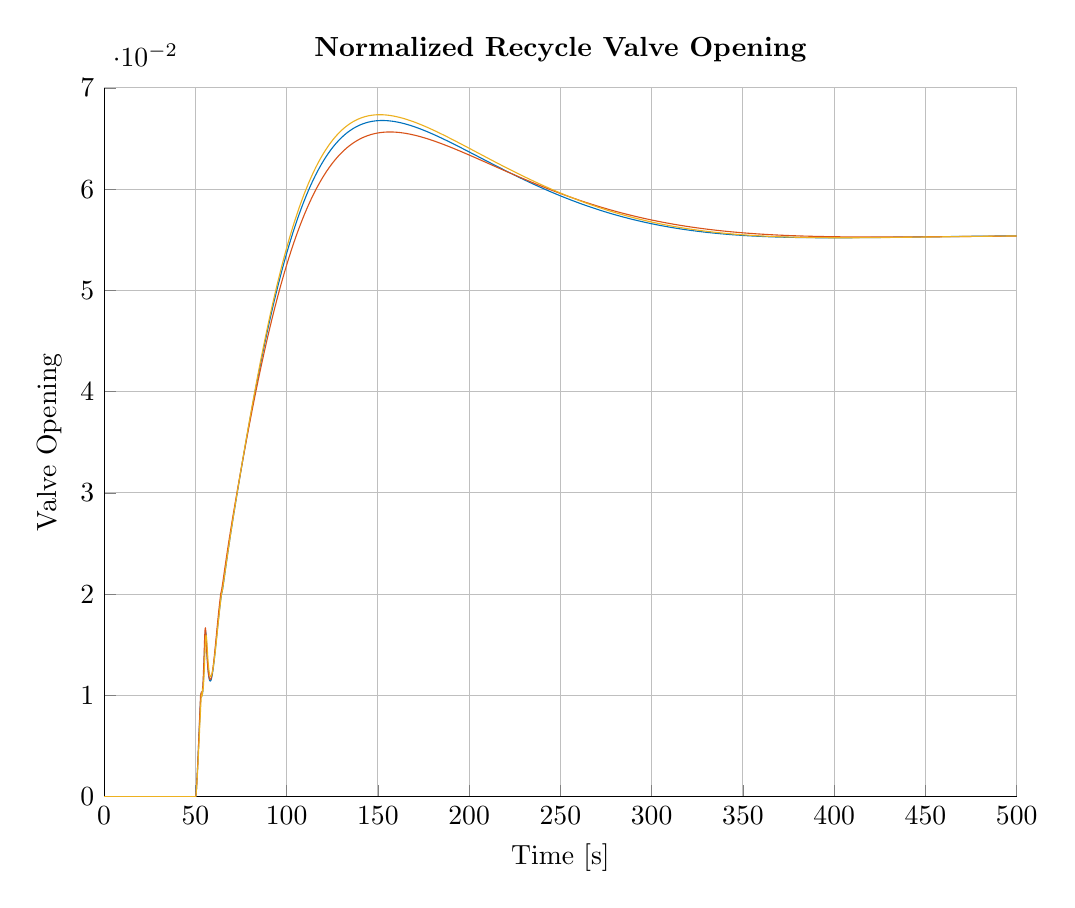
\begin{tikzpicture}

\begin{axis}[%
width=4.563in,
height=3.544in,
at={(0.792in,0.541in)},
scale only axis,
xmin=0,
xmax=500,
xlabel={Time [s]},
xmajorgrids,
ymin=0,
ymax=0.07,
ylabel={Valve Opening},
ymajorgrids,
axis background/.style={fill=white},
title style={font=\bfseries},
title={Normalized Recycle Valve Opening},
axis x line*=bottom,
axis y line*=left
]
\addplot [color=mycolor1,solid,forget plot]
  table[row sep=crcr]{%
0	6.90949e-310\\
0.05	6.90949e-310\\
0.1	6.90949e-310\\
0.15	6.90949e-310\\
0.2	6.90949e-310\\
0.25	6.90949e-310\\
0.3	6.90949e-310\\
0.35	6.90949e-310\\
0.4	6.90949e-310\\
0.45	6.90949e-310\\
0.5	6.90949e-310\\
0.55	6.90949e-310\\
0.6	6.90949e-310\\
0.65	6.90949e-310\\
0.7	6.90949e-310\\
0.75	6.90949e-310\\
0.8	6.90949e-310\\
0.85	6.90949e-310\\
0.9	6.90949e-310\\
0.95	6.90949e-310\\
1	6.90949e-310\\
1.05	6.90949e-310\\
1.1	6.90949e-310\\
1.15	6.90949e-310\\
1.2	6.90949e-310\\
1.25	6.90949e-310\\
1.3	6.90949e-310\\
1.35	6.90949e-310\\
1.4	6.90949e-310\\
1.45	6.90949e-310\\
1.5	6.90949e-310\\
1.55	6.90949e-310\\
1.6	6.90949e-310\\
1.65	6.90949e-310\\
1.7	6.90949e-310\\
1.75	6.90949e-310\\
1.8	6.90949e-310\\
1.85	6.90949e-310\\
1.9	6.90949e-310\\
1.95	6.90949e-310\\
2	6.90949e-310\\
2.05	6.90949e-310\\
2.1	6.90949e-310\\
2.15	6.90949e-310\\
2.2	6.90949e-310\\
2.25	6.90949e-310\\
2.3	6.90949e-310\\
2.35	6.90949e-310\\
2.4	6.90949e-310\\
2.45	6.90949e-310\\
2.5	6.90949e-310\\
2.55	6.90949e-310\\
2.6	6.90949e-310\\
2.65	6.90949e-310\\
2.7	6.90949e-310\\
2.75	6.90949e-310\\
2.8	6.90949e-310\\
2.85	6.90949e-310\\
2.9	6.90949e-310\\
2.95	6.90949e-310\\
3	6.90949e-310\\
3.05	6.90949e-310\\
3.1	6.90949e-310\\
3.15	6.90949e-310\\
3.2	6.90949e-310\\
3.25	6.90949e-310\\
3.3	6.90949e-310\\
3.35	6.90949e-310\\
3.4	6.90949e-310\\
3.45	6.90949e-310\\
3.5	6.90949e-310\\
3.55	6.90949e-310\\
3.6	6.90949e-310\\
3.65	6.90949e-310\\
3.7	6.90949e-310\\
3.75	6.90949e-310\\
3.8	6.90949e-310\\
3.85	6.90949e-310\\
3.9	6.90949e-310\\
3.95	6.90949e-310\\
4	6.90949e-310\\
4.05	6.90949e-310\\
4.1	6.90949e-310\\
4.15	6.90949e-310\\
4.2	6.90949e-310\\
4.25	6.90949e-310\\
4.3	6.90949e-310\\
4.35	6.90949e-310\\
4.4	6.90949e-310\\
4.45	6.90949e-310\\
4.5	6.90949e-310\\
4.55	6.90949e-310\\
4.6	6.90949e-310\\
4.65	6.90949e-310\\
4.7	6.90949e-310\\
4.75	6.90949e-310\\
4.8	6.90949e-310\\
4.85	6.90949e-310\\
4.9	6.90949e-310\\
4.95	6.90949e-310\\
5	6.90949e-310\\
5.05	6.90949e-310\\
5.1	6.90949e-310\\
5.15	6.90949e-310\\
5.2	6.90949e-310\\
5.25	6.90949e-310\\
5.3	6.90949e-310\\
5.35	6.90949e-310\\
5.4	6.90949e-310\\
5.45	6.90949e-310\\
5.5	6.90949e-310\\
5.55	6.90949e-310\\
5.6	6.90949e-310\\
5.65	6.90949e-310\\
5.7	6.90949e-310\\
5.75	6.90949e-310\\
5.8	6.90949e-310\\
5.85	6.90949e-310\\
5.9	6.90949e-310\\
5.95	6.90949e-310\\
6	6.90949e-310\\
6.05	6.90949e-310\\
6.1	6.90949e-310\\
6.15	6.90949e-310\\
6.2	6.90949e-310\\
6.25	6.90949e-310\\
6.3	6.90949e-310\\
6.35	6.90949e-310\\
6.4	6.90949e-310\\
6.45	6.90949e-310\\
6.5	6.90949e-310\\
6.55	6.90949e-310\\
6.6	6.90949e-310\\
6.65	6.90949e-310\\
6.7	6.90949e-310\\
6.75	6.90949e-310\\
6.8	6.90949e-310\\
6.85	6.90949e-310\\
6.9	6.90949e-310\\
6.95	6.90949e-310\\
7	6.90949e-310\\
7.05	6.90949e-310\\
7.1	6.90949e-310\\
7.15	6.90949e-310\\
7.2	6.90949e-310\\
7.25	6.90949e-310\\
7.3	6.90949e-310\\
7.35	6.90949e-310\\
7.4	6.90949e-310\\
7.45	6.90949e-310\\
7.5	6.90949e-310\\
7.55	6.90949e-310\\
7.6	6.90949e-310\\
7.65	6.90949e-310\\
7.7	6.90949e-310\\
7.75	6.90949e-310\\
7.8	6.90949e-310\\
7.85	6.90949e-310\\
7.9	6.90949e-310\\
7.95	6.90949e-310\\
8	6.90949e-310\\
8.05	6.90949e-310\\
8.1	6.90949e-310\\
8.15	6.90949e-310\\
8.2	6.90949e-310\\
8.25	6.90949e-310\\
8.3	6.90949e-310\\
8.35	6.90949e-310\\
8.4	6.90949e-310\\
8.45	6.90949e-310\\
8.5	6.90949e-310\\
8.55	6.90949e-310\\
8.6	6.90949e-310\\
8.65	6.90949e-310\\
8.7	6.90949e-310\\
8.75	6.90949e-310\\
8.8	6.90949e-310\\
8.85	6.90949e-310\\
8.9	6.90949e-310\\
8.95	6.90949e-310\\
9	6.90949e-310\\
9.05	6.90949e-310\\
9.1	6.90949e-310\\
9.15	6.90949e-310\\
9.2	6.90949e-310\\
9.25	6.90949e-310\\
9.3	6.90949e-310\\
9.35	6.90949e-310\\
9.4	6.90949e-310\\
9.45	6.90949e-310\\
9.5	6.90949e-310\\
9.55	6.90949e-310\\
9.6	6.90949e-310\\
9.65	6.90949e-310\\
9.7	6.90949e-310\\
9.75	6.90949e-310\\
9.8	6.90949e-310\\
9.85	6.90949e-310\\
9.9	6.90949e-310\\
9.95	6.90949e-310\\
10	6.90949e-310\\
10.05	6.90949e-310\\
10.1	6.90949e-310\\
10.15	6.90949e-310\\
10.2	6.90949e-310\\
10.25	6.90949e-310\\
10.3	6.90949e-310\\
10.35	6.90949e-310\\
10.4	6.90949e-310\\
10.45	6.90949e-310\\
10.5	6.90949e-310\\
10.55	6.90949e-310\\
10.6	6.90949e-310\\
10.65	6.90949e-310\\
10.7	6.90949e-310\\
10.75	6.90949e-310\\
10.8	6.90949e-310\\
10.85	6.90949e-310\\
10.9	6.90949e-310\\
10.95	6.90949e-310\\
11	6.90949e-310\\
11.05	6.90949e-310\\
11.1	6.90949e-310\\
11.15	6.90949e-310\\
11.2	6.90949e-310\\
11.25	6.90949e-310\\
11.3	6.90949e-310\\
11.35	6.90949e-310\\
11.4	6.90949e-310\\
11.45	6.90949e-310\\
11.5	6.90949e-310\\
11.55	6.90949e-310\\
11.6	6.90949e-310\\
11.65	6.90949e-310\\
11.7	6.90949e-310\\
11.75	6.90949e-310\\
11.8	6.90949e-310\\
11.85	6.90949e-310\\
11.9	6.90949e-310\\
11.95	6.90949e-310\\
12	6.90949e-310\\
12.05	6.90949e-310\\
12.1	6.90949e-310\\
12.15	6.90949e-310\\
12.2	6.90949e-310\\
12.25	6.90949e-310\\
12.3	6.90949e-310\\
12.35	6.90949e-310\\
12.4	6.90949e-310\\
12.45	6.90949e-310\\
12.5	6.90949e-310\\
12.55	6.90949e-310\\
12.6	6.90949e-310\\
12.65	6.90949e-310\\
12.7	6.90949e-310\\
12.75	6.90949e-310\\
12.8	6.90949e-310\\
12.85	6.90949e-310\\
12.9	6.90949e-310\\
12.95	6.90949e-310\\
13	6.90949e-310\\
13.05	6.90949e-310\\
13.1	6.90949e-310\\
13.15	6.90949e-310\\
13.2	6.90949e-310\\
13.25	6.90949e-310\\
13.3	6.90949e-310\\
13.35	6.90949e-310\\
13.4	6.90949e-310\\
13.45	6.90949e-310\\
13.5	6.90949e-310\\
13.55	6.90949e-310\\
13.6	6.90949e-310\\
13.65	6.90949e-310\\
13.7	6.90949e-310\\
13.75	6.90949e-310\\
13.8	6.90949e-310\\
13.85	6.90949e-310\\
13.9	6.90949e-310\\
13.95	6.90949e-310\\
14	6.90949e-310\\
14.05	6.90949e-310\\
14.1	6.90949e-310\\
14.15	6.90949e-310\\
14.2	6.90949e-310\\
14.25	6.90949e-310\\
14.3	6.90949e-310\\
14.35	6.90949e-310\\
14.4	6.90949e-310\\
14.45	6.90949e-310\\
14.5	6.90949e-310\\
14.55	6.90949e-310\\
14.6	6.90949e-310\\
14.65	6.90949e-310\\
14.7	6.90949e-310\\
14.75	6.90949e-310\\
14.8	6.90949e-310\\
14.85	6.90949e-310\\
14.9	6.90949e-310\\
14.95	6.90949e-310\\
15	6.90949e-310\\
15.05	6.90949e-310\\
15.1	6.90949e-310\\
15.15	6.90949e-310\\
15.2	6.90949e-310\\
15.25	6.90949e-310\\
15.3	6.90949e-310\\
15.35	6.90949e-310\\
15.4	6.90949e-310\\
15.45	6.90949e-310\\
15.5	6.90949e-310\\
15.55	6.90949e-310\\
15.6	6.90949e-310\\
15.65	6.90949e-310\\
15.7	6.90949e-310\\
15.75	6.90949e-310\\
15.8	6.90949e-310\\
15.85	6.90949e-310\\
15.9	6.90949e-310\\
15.95	6.90949e-310\\
16	6.90949e-310\\
16.05	6.90949e-310\\
16.1	6.90949e-310\\
16.15	6.90949e-310\\
16.2	6.90949e-310\\
16.25	6.90949e-310\\
16.3	6.90949e-310\\
16.35	6.90949e-310\\
16.4	6.90949e-310\\
16.45	6.90949e-310\\
16.5	6.90949e-310\\
16.55	6.90949e-310\\
16.6	6.90949e-310\\
16.65	6.90949e-310\\
16.7	6.90949e-310\\
16.75	6.90949e-310\\
16.8	6.90949e-310\\
16.85	6.90949e-310\\
16.9	6.90949e-310\\
16.95	6.90949e-310\\
17	6.90949e-310\\
17.05	6.90949e-310\\
17.1	6.90949e-310\\
17.15	6.90949e-310\\
17.2	6.90949e-310\\
17.25	6.90949e-310\\
17.3	6.90949e-310\\
17.35	6.90949e-310\\
17.4	6.90949e-310\\
17.45	6.90949e-310\\
17.5	6.90949e-310\\
17.55	6.90949e-310\\
17.6	6.90949e-310\\
17.65	6.90949e-310\\
17.7	6.90949e-310\\
17.75	6.90949e-310\\
17.8	6.90949e-310\\
17.85	6.90949e-310\\
17.9	6.90949e-310\\
17.95	6.90949e-310\\
18	6.90949e-310\\
18.05	6.90949e-310\\
18.1	6.90949e-310\\
18.15	6.90949e-310\\
18.2	6.90949e-310\\
18.25	6.90949e-310\\
18.3	6.90949e-310\\
18.35	6.90949e-310\\
18.4	6.90949e-310\\
18.45	6.90949e-310\\
18.5	6.90949e-310\\
18.55	6.90949e-310\\
18.6	6.90949e-310\\
18.65	6.90949e-310\\
18.7	6.90949e-310\\
18.75	6.90949e-310\\
18.8	6.90949e-310\\
18.85	6.90949e-310\\
18.9	6.90949e-310\\
18.95	6.90949e-310\\
19	6.90949e-310\\
19.05	6.90949e-310\\
19.1	6.90949e-310\\
19.15	6.90949e-310\\
19.2	6.90949e-310\\
19.25	6.90949e-310\\
19.3	6.90949e-310\\
19.35	6.90949e-310\\
19.4	6.90949e-310\\
19.45	6.90949e-310\\
19.5	6.90949e-310\\
19.55	6.90949e-310\\
19.6	6.90949e-310\\
19.65	6.90949e-310\\
19.7	6.90949e-310\\
19.75	6.90949e-310\\
19.8	6.90949e-310\\
19.85	6.90949e-310\\
19.9	6.90949e-310\\
19.95	6.90949e-310\\
20	6.90949e-310\\
20.05	6.90949e-310\\
20.1	6.90949e-310\\
20.15	6.90949e-310\\
20.2	6.90949e-310\\
20.25	6.90949e-310\\
20.3	6.90949e-310\\
20.35	6.90949e-310\\
20.4	6.90949e-310\\
20.45	6.90949e-310\\
20.5	6.90949e-310\\
20.55	6.90949e-310\\
20.6	6.90949e-310\\
20.65	6.90949e-310\\
20.7	6.90949e-310\\
20.75	6.90949e-310\\
20.8	6.90949e-310\\
20.85	6.90949e-310\\
20.9	6.90949e-310\\
20.95	6.90949e-310\\
21	6.90949e-310\\
21.05	6.90949e-310\\
21.1	6.90949e-310\\
21.15	6.90949e-310\\
21.2	6.90949e-310\\
21.25	6.90949e-310\\
21.3	6.90949e-310\\
21.35	6.90949e-310\\
21.4	6.90949e-310\\
21.45	6.90949e-310\\
21.5	6.90949e-310\\
21.55	6.90949e-310\\
21.6	6.90949e-310\\
21.65	6.90949e-310\\
21.7	6.90949e-310\\
21.75	6.90949e-310\\
21.8	6.90949e-310\\
21.85	6.90949e-310\\
21.9	6.90949e-310\\
21.95	6.90949e-310\\
22	6.90949e-310\\
22.05	6.90949e-310\\
22.1	6.90949e-310\\
22.15	6.90949e-310\\
22.2	6.90949e-310\\
22.25	6.90949e-310\\
22.3	6.90949e-310\\
22.35	6.90949e-310\\
22.4	6.90949e-310\\
22.45	6.90949e-310\\
22.5	6.90949e-310\\
22.55	6.90949e-310\\
22.6	6.90949e-310\\
22.65	6.90949e-310\\
22.7	6.90949e-310\\
22.75	6.90949e-310\\
22.8	6.90949e-310\\
22.85	6.90949e-310\\
22.9	6.90949e-310\\
22.95	6.90949e-310\\
23	6.90949e-310\\
23.05	6.90949e-310\\
23.1	6.90949e-310\\
23.15	6.90949e-310\\
23.2	6.90949e-310\\
23.25	6.90949e-310\\
23.3	6.90949e-310\\
23.35	6.90949e-310\\
23.4	6.90949e-310\\
23.45	6.90949e-310\\
23.5	6.90949e-310\\
23.55	6.90949e-310\\
23.6	6.90949e-310\\
23.65	6.90949e-310\\
23.7	6.90949e-310\\
23.75	6.90949e-310\\
23.8	6.90949e-310\\
23.85	6.90949e-310\\
23.9	6.90949e-310\\
23.95	6.90949e-310\\
24	6.90949e-310\\
24.05	6.90949e-310\\
24.1	6.90949e-310\\
24.15	6.90949e-310\\
24.2	6.90949e-310\\
24.25	6.90949e-310\\
24.3	6.90949e-310\\
24.35	6.90949e-310\\
24.4	6.90949e-310\\
24.45	6.90949e-310\\
24.5	6.90949e-310\\
24.55	6.90949e-310\\
24.6	6.90949e-310\\
24.65	6.90949e-310\\
24.7	6.90949e-310\\
24.75	6.90949e-310\\
24.8	6.90949e-310\\
24.85	6.90949e-310\\
24.9	6.90949e-310\\
24.95	6.90949e-310\\
25	6.90949e-310\\
25.05	6.90949e-310\\
25.1	6.90949e-310\\
25.15	6.90949e-310\\
25.2	6.90949e-310\\
25.25	6.90949e-310\\
25.3	6.90949e-310\\
25.35	6.90949e-310\\
25.4	6.90949e-310\\
25.45	6.90949e-310\\
25.5	6.90949e-310\\
25.55	6.90949e-310\\
25.6	6.90949e-310\\
25.65	6.90949e-310\\
25.7	6.90949e-310\\
25.75	6.90949e-310\\
25.8	6.90949e-310\\
25.85	6.90949e-310\\
25.9	6.90949e-310\\
25.95	6.90949e-310\\
26	6.90949e-310\\
26.05	6.90949e-310\\
26.1	6.90949e-310\\
26.15	6.90949e-310\\
26.2	6.90949e-310\\
26.25	6.90949e-310\\
26.3	6.90949e-310\\
26.35	6.90949e-310\\
26.4	6.90949e-310\\
26.45	6.90949e-310\\
26.5	6.90949e-310\\
26.55	6.90949e-310\\
26.6	6.90949e-310\\
26.65	6.90949e-310\\
26.7	6.90949e-310\\
26.75	6.90949e-310\\
26.8	6.90949e-310\\
26.85	6.90949e-310\\
26.9	6.90949e-310\\
26.95	6.90949e-310\\
27	6.90949e-310\\
27.05	6.90949e-310\\
27.1	6.90949e-310\\
27.15	6.90949e-310\\
27.2	6.90949e-310\\
27.25	6.90949e-310\\
27.3	6.90949e-310\\
27.35	6.90949e-310\\
27.4	6.90949e-310\\
27.45	6.90949e-310\\
27.5	6.90949e-310\\
27.55	6.90949e-310\\
27.6	6.90949e-310\\
27.65	6.90949e-310\\
27.7	6.90949e-310\\
27.75	6.90949e-310\\
27.8	6.90949e-310\\
27.85	6.90949e-310\\
27.9	6.90949e-310\\
27.95	6.90949e-310\\
28	6.90949e-310\\
28.05	6.90949e-310\\
28.1	6.90949e-310\\
28.15	6.90949e-310\\
28.2	6.90949e-310\\
28.25	6.90949e-310\\
28.3	6.90949e-310\\
28.35	6.90949e-310\\
28.4	6.90949e-310\\
28.45	6.90949e-310\\
28.5	6.90949e-310\\
28.55	6.90949e-310\\
28.6	6.90949e-310\\
28.65	6.90949e-310\\
28.7	6.90949e-310\\
28.75	6.90949e-310\\
28.8	6.90949e-310\\
28.85	6.90949e-310\\
28.9	6.90949e-310\\
28.95	6.90949e-310\\
29	6.90949e-310\\
29.05	6.90949e-310\\
29.1	6.90949e-310\\
29.15	6.90949e-310\\
29.2	6.90949e-310\\
29.25	6.90949e-310\\
29.3	6.90949e-310\\
29.35	6.90949e-310\\
29.4	6.90949e-310\\
29.45	6.90949e-310\\
29.5	6.90949e-310\\
29.55	6.90949e-310\\
29.6	6.90949e-310\\
29.65	6.90949e-310\\
29.7	6.90949e-310\\
29.75	6.90949e-310\\
29.8	6.90949e-310\\
29.85	6.90949e-310\\
29.9	6.90949e-310\\
29.95	6.90949e-310\\
30	6.90949e-310\\
30.05	6.90949e-310\\
30.1	6.90949e-310\\
30.15	6.90949e-310\\
30.2	6.90949e-310\\
30.25	6.90949e-310\\
30.3	6.90949e-310\\
30.35	6.90949e-310\\
30.4	6.90949e-310\\
30.45	6.90949e-310\\
30.5	6.90949e-310\\
30.55	6.90949e-310\\
30.6	6.90949e-310\\
30.65	6.90949e-310\\
30.7	6.90949e-310\\
30.75	6.90949e-310\\
30.8	6.90949e-310\\
30.85	6.90949e-310\\
30.9	6.90949e-310\\
30.95	6.90949e-310\\
31	6.90949e-310\\
31.05	6.90949e-310\\
31.1	6.90949e-310\\
31.15	6.90949e-310\\
31.2	6.90949e-310\\
31.25	6.90949e-310\\
31.3	6.90949e-310\\
31.35	6.90949e-310\\
31.4	6.90949e-310\\
31.45	6.90949e-310\\
31.5	6.90949e-310\\
31.55	6.90949e-310\\
31.6	6.90949e-310\\
31.65	6.90949e-310\\
31.7	6.90949e-310\\
31.75	6.90949e-310\\
31.8	6.90949e-310\\
31.85	6.90949e-310\\
31.9	6.90949e-310\\
31.95	6.90949e-310\\
32	6.90949e-310\\
32.05	6.90949e-310\\
32.1	6.90949e-310\\
32.15	6.90949e-310\\
32.2	6.90949e-310\\
32.25	6.90949e-310\\
32.3	6.90949e-310\\
32.35	6.90949e-310\\
32.4	6.90949e-310\\
32.45	6.90949e-310\\
32.5	6.90949e-310\\
32.55	6.90949e-310\\
32.6	6.90949e-310\\
32.65	6.90949e-310\\
32.7	6.90949e-310\\
32.75	6.90949e-310\\
32.8	6.90949e-310\\
32.85	6.90949e-310\\
32.9	6.90949e-310\\
32.95	6.90949e-310\\
33	6.90949e-310\\
33.05	6.90949e-310\\
33.1	6.90949e-310\\
33.15	6.90949e-310\\
33.2	6.90949e-310\\
33.25	6.90949e-310\\
33.3	6.90949e-310\\
33.35	6.90949e-310\\
33.4	6.90949e-310\\
33.45	6.90949e-310\\
33.5	6.90949e-310\\
33.55	6.90949e-310\\
33.6	6.90949e-310\\
33.65	6.90949e-310\\
33.7	6.90949e-310\\
33.75	6.90949e-310\\
33.8	6.90949e-310\\
33.85	6.90949e-310\\
33.9	6.90949e-310\\
33.95	6.90949e-310\\
34	6.90949e-310\\
34.05	6.90949e-310\\
34.1	6.90949e-310\\
34.15	6.90949e-310\\
34.2	6.90949e-310\\
34.25	6.90949e-310\\
34.3	6.90949e-310\\
34.35	6.90949e-310\\
34.4	6.90949e-310\\
34.45	6.90949e-310\\
34.5	6.90949e-310\\
34.55	6.90949e-310\\
34.6	6.90949e-310\\
34.65	6.90949e-310\\
34.7	6.90949e-310\\
34.75	6.90949e-310\\
34.8	6.90949e-310\\
34.85	6.90949e-310\\
34.9	6.90949e-310\\
34.95	6.90949e-310\\
35	6.90949e-310\\
35.05	6.90949e-310\\
35.1	6.90949e-310\\
35.15	6.90949e-310\\
35.2	6.90949e-310\\
35.25	6.90949e-310\\
35.3	6.90949e-310\\
35.35	6.90949e-310\\
35.4	6.90949e-310\\
35.45	6.90949e-310\\
35.5	6.90949e-310\\
35.55	6.90949e-310\\
35.6	6.90949e-310\\
35.65	6.90949e-310\\
35.7	6.90949e-310\\
35.75	6.90949e-310\\
35.8	6.90949e-310\\
35.85	6.90949e-310\\
35.9	6.90949e-310\\
35.95	6.90949e-310\\
36	6.90949e-310\\
36.05	6.90949e-310\\
36.1	6.90949e-310\\
36.15	6.90949e-310\\
36.2	6.90949e-310\\
36.25	6.90949e-310\\
36.3	6.90949e-310\\
36.35	6.90949e-310\\
36.4	6.90949e-310\\
36.45	6.90949e-310\\
36.5	6.90949e-310\\
36.55	6.90949e-310\\
36.6	6.90949e-310\\
36.65	6.90949e-310\\
36.7	6.90949e-310\\
36.75	6.90949e-310\\
36.8	6.90949e-310\\
36.85	6.90949e-310\\
36.9	6.90949e-310\\
36.95	6.90949e-310\\
37	6.90949e-310\\
37.05	6.90949e-310\\
37.1	6.90949e-310\\
37.15	6.90949e-310\\
37.2	6.90949e-310\\
37.25	6.90949e-310\\
37.3	6.90949e-310\\
37.35	6.90949e-310\\
37.4	6.90949e-310\\
37.45	6.90949e-310\\
37.5	6.90949e-310\\
37.55	6.90949e-310\\
37.6	6.90949e-310\\
37.65	6.90949e-310\\
37.7	6.90949e-310\\
37.75	6.90949e-310\\
37.8	6.90949e-310\\
37.85	6.90949e-310\\
37.9	6.90949e-310\\
37.95	6.90949e-310\\
38	6.90949e-310\\
38.05	6.90949e-310\\
38.1	6.90949e-310\\
38.15	6.90949e-310\\
38.2	6.90949e-310\\
38.25	6.90949e-310\\
38.3	6.90949e-310\\
38.35	6.90949e-310\\
38.4	6.90949e-310\\
38.45	6.90949e-310\\
38.5	6.90949e-310\\
38.55	6.90949e-310\\
38.6	6.90949e-310\\
38.65	6.90949e-310\\
38.7	6.90949e-310\\
38.75	6.90949e-310\\
38.8	6.90949e-310\\
38.85	6.90949e-310\\
38.9	6.90949e-310\\
38.95	6.90949e-310\\
39	6.90949e-310\\
39.05	6.90949e-310\\
39.1	6.90949e-310\\
39.15	6.90949e-310\\
39.2	6.90949e-310\\
39.25	6.90949e-310\\
39.3	6.90949e-310\\
39.35	6.90949e-310\\
39.4	6.90949e-310\\
39.45	6.90949e-310\\
39.5	6.90949e-310\\
39.55	6.90949e-310\\
39.6	6.90949e-310\\
39.65	6.90949e-310\\
39.7	6.90949e-310\\
39.75	6.90949e-310\\
39.8	6.90949e-310\\
39.85	6.90949e-310\\
39.9	6.90949e-310\\
39.95	6.90949e-310\\
40	6.90949e-310\\
40.05	6.90949e-310\\
40.1	6.90949e-310\\
40.15	6.90949e-310\\
40.2	6.90949e-310\\
40.25	6.90949e-310\\
40.3	6.90949e-310\\
40.35	6.90949e-310\\
40.4	6.90949e-310\\
40.45	6.90949e-310\\
40.5	6.90949e-310\\
40.55	6.90949e-310\\
40.6	6.90949e-310\\
40.65	6.90949e-310\\
40.7	6.90949e-310\\
40.75	6.90949e-310\\
40.8	6.90949e-310\\
40.85	6.90949e-310\\
40.9	6.90949e-310\\
40.95	6.90949e-310\\
41	6.90949e-310\\
41.05	6.90949e-310\\
41.1	6.90949e-310\\
41.15	6.90949e-310\\
41.2	6.90949e-310\\
41.25	6.90949e-310\\
41.3	6.90949e-310\\
41.35	6.90949e-310\\
41.4	6.90949e-310\\
41.45	6.90949e-310\\
41.5	6.90949e-310\\
41.55	6.90949e-310\\
41.6	6.90949e-310\\
41.65	6.90949e-310\\
41.7	6.90949e-310\\
41.75	6.90949e-310\\
41.8	6.90949e-310\\
41.85	6.90949e-310\\
41.9	6.90949e-310\\
41.95	6.90949e-310\\
42	6.90949e-310\\
42.05	6.90949e-310\\
42.1	6.90949e-310\\
42.15	6.90949e-310\\
42.2	6.90949e-310\\
42.25	6.90949e-310\\
42.3	6.90949e-310\\
42.35	6.90949e-310\\
42.4	6.90949e-310\\
42.45	6.90949e-310\\
42.5	6.90949e-310\\
42.55	6.90949e-310\\
42.6	6.90949e-310\\
42.65	6.90949e-310\\
42.7	6.90949e-310\\
42.75	6.90949e-310\\
42.8	6.90949e-310\\
42.85	6.90949e-310\\
42.9	6.90949e-310\\
42.95	6.90949e-310\\
43	6.90949e-310\\
43.05	6.90949e-310\\
43.1	6.90949e-310\\
43.15	6.90949e-310\\
43.2	6.90949e-310\\
43.25	6.90949e-310\\
43.3	6.90949e-310\\
43.35	6.90949e-310\\
43.4	6.90949e-310\\
43.45	6.90949e-310\\
43.5	6.90949e-310\\
43.55	6.90949e-310\\
43.6	6.90949e-310\\
43.65	6.90949e-310\\
43.7	6.90949e-310\\
43.75	6.90949e-310\\
43.8	6.90949e-310\\
43.85	6.90949e-310\\
43.9	6.90949e-310\\
43.95	6.90949e-310\\
44	6.90949e-310\\
44.05	6.90949e-310\\
44.1	6.90949e-310\\
44.15	6.90949e-310\\
44.2	6.90949e-310\\
44.25	6.90949e-310\\
44.3	6.90949e-310\\
44.35	6.90949e-310\\
44.4	6.90949e-310\\
44.45	6.90949e-310\\
44.5	6.90949e-310\\
44.55	6.90949e-310\\
44.6	6.90949e-310\\
44.65	6.90949e-310\\
44.7	6.90949e-310\\
44.75	6.90949e-310\\
44.8	6.90949e-310\\
44.85	6.90949e-310\\
44.9	6.90949e-310\\
44.95	6.90949e-310\\
45	6.90949e-310\\
45.05	6.90949e-310\\
45.1	6.90949e-310\\
45.15	6.90949e-310\\
45.2	6.90949e-310\\
45.25	6.90949e-310\\
45.3	6.90949e-310\\
45.35	6.90949e-310\\
45.4	6.90949e-310\\
45.45	6.90949e-310\\
45.5	6.90949e-310\\
45.55	6.90949e-310\\
45.6	6.90949e-310\\
45.65	6.90949e-310\\
45.7	6.90949e-310\\
45.75	6.90949e-310\\
45.8	6.90949e-310\\
45.85	6.90949e-310\\
45.9	6.90949e-310\\
45.95	6.90949e-310\\
46	6.90949e-310\\
46.05	6.90949e-310\\
46.1	6.90949e-310\\
46.15	6.90949e-310\\
46.2	6.90949e-310\\
46.25	6.90949e-310\\
46.3	6.90949e-310\\
46.35	6.90949e-310\\
46.4	6.90949e-310\\
46.45	6.90949e-310\\
46.5	6.90949e-310\\
46.55	6.90949e-310\\
46.6	6.90949e-310\\
46.65	6.90949e-310\\
46.7	6.90949e-310\\
46.75	6.90949e-310\\
46.8	6.90949e-310\\
46.85	6.90949e-310\\
46.9	6.90949e-310\\
46.95	6.90949e-310\\
47	6.90949e-310\\
47.05	6.90949e-310\\
47.1	6.90949e-310\\
47.15	6.90949e-310\\
47.2	6.90949e-310\\
47.25	6.90949e-310\\
47.3	6.90949e-310\\
47.35	6.90949e-310\\
47.4	6.90949e-310\\
47.45	6.90949e-310\\
47.5	6.90949e-310\\
47.55	6.90949e-310\\
47.6	6.90949e-310\\
47.65	6.90949e-310\\
47.7	6.90949e-310\\
47.75	6.90949e-310\\
47.8	6.90949e-310\\
47.85	6.90949e-310\\
47.9	6.90949e-310\\
47.95	6.90949e-310\\
48	6.90949e-310\\
48.05	6.90949e-310\\
48.1	6.90949e-310\\
48.15	6.90949e-310\\
48.2	6.90949e-310\\
48.25	6.90949e-310\\
48.3	6.90949e-310\\
48.35	6.90949e-310\\
48.4	6.90949e-310\\
48.45	6.90949e-310\\
48.5	6.90949e-310\\
48.55	6.90949e-310\\
48.6	6.90949e-310\\
48.65	6.90949e-310\\
48.7	6.90949e-310\\
48.75	6.90949e-310\\
48.8	6.90949e-310\\
48.85	6.90949e-310\\
48.9	6.90949e-310\\
48.95	6.90949e-310\\
49	6.90949e-310\\
49.05	6.90949e-310\\
49.1	6.90949e-310\\
49.15	6.90949e-310\\
49.2	6.90949e-310\\
49.25	6.90949e-310\\
49.3	6.90949e-310\\
49.35	6.90949e-310\\
49.4	6.90949e-310\\
49.45	6.90949e-310\\
49.5	6.90949e-310\\
49.55	6.90949e-310\\
49.6	6.90949e-310\\
49.65	6.90949e-310\\
49.7	6.90949e-310\\
49.75	6.90949e-310\\
49.8	6.90949e-310\\
49.85	6.90949e-310\\
49.9	6.90949e-310\\
49.95	6.90949e-310\\
50	6.90949e-310\\
50.05	6.90949e-310\\
50.1	1.70778e-06\\
50.15	1.05264e-05\\
50.2	3.12231e-05\\
50.25	6.733e-05\\
50.3	0.000120942\\
50.35	0.000192783\\
50.4	0.000282421\\
50.45	0.000388554\\
50.5	0.000509304\\
50.55	0.000642488\\
50.6	0.000785864\\
50.65	0.000937311\\
50.7	0.00109497\\
50.75	0.00125732\\
50.8	0.00142322\\
50.85	0.00159189\\
50.9	0.00176289\\
50.95	0.00193604\\
51	0.00211134\\
51.05	0.00228894\\
51.1	0.00246901\\
51.15	0.00265174\\
51.2	0.0028373\\
51.25	0.00302577\\
51.3	0.00321715\\
51.35	0.00341139\\
51.4	0.00360834\\
51.45	0.00380781\\
51.5	0.00400956\\
51.55	0.00421331\\
51.6	0.00441879\\
51.65	0.00462572\\
51.7	0.00483381\\
51.75	0.00504281\\
51.8	0.00525246\\
51.85	0.00546256\\
51.9	0.00567289\\
51.95	0.00588325\\
52	0.00609347\\
52.05	0.00630339\\
52.1	0.00651283\\
52.15	0.00672165\\
52.2	0.00692967\\
52.25	0.00713677\\
52.3	0.0073428\\
52.35	0.00754766\\
52.4	0.00775124\\
52.45	0.0079535\\
52.5	0.00815443\\
52.55	0.00835403\\
52.6	0.00855239\\
52.65	0.00874958\\
52.7	0.00894573\\
52.75	0.00914098\\
52.8	0.00933549\\
52.85	0.00952941\\
52.9	0.0097229\\
52.95	0.0099161\\
53	0.0101092\\
53.05	0.00982871\\
53.1	0.0100238\\
53.15	0.00976125\\
53.2	0.00999392\\
53.25	0.0102592\\
53.3	0.0100459\\
53.35	0.00985418\\
53.4	0.0101992\\
53.45	0.0100502\\
53.5	0.00992427\\
53.55	0.0103668\\
53.6	0.0102812\\
53.65	0.0102134\\
53.7	0.0101644\\
53.75	0.0101356\\
53.8	0.0101285\\
53.85	0.0101434\\
53.9	0.0101803\\
53.95	0.0102384\\
54	0.0103164\\
54.05	0.0104126\\
54.1	0.0105254\\
54.15	0.0106531\\
54.2	0.0107941\\
54.25	0.0109471\\
54.3	0.0111109\\
54.35	0.0112848\\
54.4	0.0114678\\
54.45	0.0116597\\
54.5	0.01186\\
54.55	0.0120684\\
54.6	0.0122847\\
54.65	0.0125087\\
54.7	0.0127403\\
54.75	0.0129794\\
54.8	0.0132258\\
54.85	0.0134794\\
54.9	0.01374\\
54.95	0.0140076\\
55	0.014282\\
55.05	0.0145587\\
55.1	0.0148275\\
55.15	0.0150826\\
55.2	0.0153151\\
55.25	0.0155271\\
55.3	0.0157193\\
55.35	0.0158837\\
55.4	0.0160168\\
55.45	0.0161225\\
55.5	0.0161968\\
55.55	0.0162411\\
55.6	0.0162635\\
55.65	0.0162633\\
55.7	0.0162386\\
55.75	0.0161878\\
55.8	0.0161105\\
55.85	0.0160075\\
55.9	0.0158808\\
55.95	0.0157336\\
56	0.0155694\\
56.05	0.0153925\\
56.1	0.0152069\\
56.15	0.0150162\\
56.2	0.0148236\\
56.25	0.0146319\\
56.3	0.014443\\
56.35	0.0142585\\
56.4	0.0140793\\
56.45	0.0139063\\
56.5	0.0137396\\
56.55	0.0135796\\
56.6	0.0134263\\
56.65	0.0132797\\
56.7	0.0131397\\
56.75	0.0130061\\
56.8	0.012879\\
56.85	0.0127582\\
56.9	0.0126435\\
56.95	0.012535\\
57	0.0124325\\
57.05	0.0123359\\
57.1	0.012245\\
57.15	0.0121598\\
57.2	0.0120801\\
57.25	0.0120057\\
57.3	0.0119366\\
57.35	0.0118724\\
57.4	0.0118132\\
57.45	0.0117586\\
57.5	0.0117086\\
57.55	0.011663\\
57.6	0.0116216\\
57.65	0.0115844\\
57.7	0.0115512\\
57.75	0.0115219\\
57.8	0.0114964\\
57.85	0.0114745\\
57.9	0.0114562\\
57.95	0.0114415\\
58	0.0114301\\
58.05	0.0114221\\
58.1	0.0114173\\
58.15	0.0114157\\
58.2	0.0114172\\
58.25	0.0114217\\
58.3	0.0114293\\
58.35	0.0114396\\
58.4	0.0114529\\
58.45	0.0114689\\
58.5	0.0114875\\
58.55	0.0115088\\
58.6	0.0115327\\
58.65	0.011559\\
58.7	0.0115878\\
58.75	0.0116189\\
58.8	0.0116523\\
58.85	0.0116879\\
58.9	0.0117256\\
58.95	0.0117655\\
59	0.0118074\\
59.05	0.0118513\\
59.1	0.0118971\\
59.15	0.0119448\\
59.2	0.0119943\\
59.25	0.0120456\\
59.3	0.0120987\\
59.35	0.0121534\\
59.4	0.0122097\\
59.45	0.0122677\\
59.5	0.0123271\\
59.55	0.0123881\\
59.6	0.0124506\\
59.65	0.0125145\\
59.7	0.0125797\\
59.75	0.0126463\\
59.8	0.0127142\\
59.85	0.0127833\\
59.9	0.0128537\\
59.95	0.0129252\\
60	0.0129979\\
60.05	0.0130717\\
60.1	0.0131465\\
60.15	0.0132224\\
60.2	0.0132992\\
60.25	0.013377\\
60.3	0.0134556\\
60.35	0.0135352\\
60.4	0.0136156\\
60.45	0.0136968\\
60.5	0.0137787\\
60.55	0.0138613\\
60.6	0.0139447\\
60.65	0.0140286\\
60.7	0.0141132\\
60.75	0.0141984\\
60.8	0.0142841\\
60.85	0.0143703\\
60.9	0.0144569\\
60.95	0.014544\\
61	0.0146315\\
61.05	0.0147193\\
61.1	0.0148075\\
61.15	0.0148959\\
61.2	0.0149846\\
61.25	0.0150735\\
61.3	0.0151626\\
61.35	0.0152519\\
61.4	0.0153412\\
61.45	0.0154307\\
61.5	0.0155202\\
61.55	0.0156097\\
61.6	0.0156992\\
61.65	0.0157887\\
61.7	0.0158781\\
61.75	0.0159674\\
61.8	0.0160566\\
61.85	0.0161456\\
61.9	0.0162345\\
61.95	0.0163231\\
62	0.0164115\\
62.05	0.0164996\\
62.1	0.0165875\\
62.15	0.016675\\
62.2	0.0167622\\
62.25	0.0168491\\
62.3	0.0169356\\
62.35	0.0170217\\
62.4	0.0171074\\
62.45	0.0171927\\
62.5	0.0172775\\
62.55	0.0173619\\
62.6	0.0174458\\
62.65	0.0175293\\
62.7	0.0176122\\
62.75	0.0176947\\
62.8	0.0177767\\
62.85	0.0178582\\
62.9	0.0179391\\
62.95	0.0180195\\
63	0.0180995\\
63.05	0.0181789\\
63.1	0.0182577\\
63.15	0.0183361\\
63.2	0.0184139\\
63.25	0.0184913\\
63.3	0.0185681\\
63.35	0.0186444\\
63.4	0.0187202\\
63.45	0.0187956\\
63.5	0.0188704\\
63.55	0.0189448\\
63.6	0.0190188\\
63.65	0.0190922\\
63.7	0.0191653\\
63.75	0.0192379\\
63.8	0.0193102\\
63.85	0.019382\\
63.9	0.0194534\\
63.95	0.0195245\\
64	0.0195952\\
64.05	0.0196656\\
64.1	0.0197357\\
64.15	0.0198054\\
64.2	0.0198748\\
64.25	0.019944\\
64.3	0.0200129\\
64.35	0.0200409\\
64.4	0.0200692\\
64.45	0.0200987\\
64.5	0.0201304\\
64.55	0.0201647\\
64.6	0.020202\\
64.65	0.0202425\\
64.7	0.0202859\\
64.75	0.0203321\\
64.8	0.0203808\\
64.85	0.0204317\\
64.9	0.0204844\\
64.95	0.0205387\\
65	0.0205944\\
65.05	0.0206512\\
65.1	0.020709\\
65.15	0.0207676\\
65.2	0.0208269\\
65.25	0.0208869\\
65.3	0.0209475\\
65.35	0.0210087\\
65.4	0.0210703\\
65.45	0.0211323\\
65.5	0.0211948\\
65.55	0.0212576\\
65.6	0.0213206\\
65.65	0.021384\\
65.7	0.0214476\\
65.75	0.0215114\\
65.8	0.0215753\\
65.85	0.0216394\\
65.9	0.0217036\\
65.95	0.0217678\\
66	0.0218322\\
66.05	0.0218966\\
66.1	0.021961\\
66.15	0.0220254\\
66.2	0.0220898\\
66.25	0.0221542\\
66.3	0.0222186\\
66.35	0.0222829\\
66.4	0.0223472\\
66.45	0.0224114\\
66.5	0.0224756\\
66.55	0.0225398\\
66.6	0.0226038\\
66.65	0.0226679\\
66.7	0.0227319\\
66.75	0.0227958\\
66.8	0.0228597\\
66.85	0.0229236\\
66.9	0.0229875\\
66.95	0.0230512\\
67	0.023115\\
67.05	0.0231786\\
67.1	0.0232422\\
67.15	0.0233057\\
67.2	0.0233691\\
67.25	0.0234324\\
67.3	0.0234956\\
67.35	0.0235586\\
67.4	0.0236216\\
67.45	0.0236844\\
67.5	0.023747\\
67.55	0.0238096\\
67.6	0.023872\\
67.65	0.0239343\\
67.7	0.0239964\\
67.75	0.0240585\\
67.8	0.0241204\\
67.85	0.0241822\\
67.9	0.0242438\\
67.95	0.0243054\\
68	0.0243668\\
68.05	0.0244281\\
68.1	0.0244892\\
68.15	0.0245503\\
68.2	0.0246112\\
68.25	0.024672\\
68.3	0.0247327\\
68.35	0.0247933\\
68.4	0.0248537\\
68.45	0.0249141\\
68.5	0.0249743\\
68.55	0.0250344\\
68.6	0.0250944\\
68.65	0.0251543\\
68.7	0.0252141\\
68.75	0.0252738\\
68.8	0.0253333\\
68.85	0.0253928\\
68.9	0.0254521\\
68.95	0.0255114\\
69	0.0255706\\
69.05	0.0256296\\
69.1	0.0256886\\
69.15	0.0257474\\
69.2	0.0258062\\
69.25	0.0258649\\
69.3	0.0259235\\
69.35	0.0259819\\
69.4	0.0260403\\
69.45	0.0260986\\
69.5	0.0261569\\
69.55	0.026215\\
69.6	0.026273\\
69.65	0.026331\\
69.7	0.0263889\\
69.75	0.0264467\\
69.8	0.0265044\\
69.85	0.0265621\\
69.9	0.0266196\\
69.95	0.0266771\\
70	0.0267345\\
70.05	0.0267919\\
70.1	0.0268491\\
70.15	0.0269063\\
70.2	0.0269634\\
70.25	0.0270205\\
70.3	0.0270775\\
70.35	0.0271344\\
70.4	0.0271913\\
70.45	0.027248\\
70.5	0.0273048\\
70.55	0.0273614\\
70.6	0.027418\\
70.65	0.0274746\\
70.7	0.027531\\
70.75	0.0275875\\
70.8	0.0276438\\
70.85	0.0277001\\
70.9	0.0277564\\
70.95	0.0278126\\
71	0.0278687\\
71.05	0.0279248\\
71.1	0.0279808\\
71.15	0.0280368\\
71.2	0.0280927\\
71.25	0.0281486\\
71.3	0.0282044\\
71.35	0.0282602\\
71.4	0.0283159\\
71.45	0.0283715\\
71.5	0.0284272\\
71.55	0.0284827\\
71.6	0.0285383\\
71.65	0.0285938\\
71.7	0.0286492\\
71.75	0.0287046\\
71.8	0.0287599\\
71.85	0.0288152\\
71.9	0.0288705\\
71.95	0.0289257\\
72	0.0289809\\
72.05	0.029036\\
72.1	0.0290911\\
72.15	0.0291462\\
72.2	0.0292012\\
72.25	0.0292562\\
72.3	0.0293111\\
72.35	0.029366\\
72.4	0.0294208\\
72.45	0.0294757\\
72.5	0.0295304\\
72.55	0.0295852\\
72.6	0.0296399\\
72.65	0.0296945\\
72.7	0.0297492\\
72.75	0.0298037\\
72.8	0.0298583\\
72.85	0.0299128\\
72.9	0.0299673\\
72.95	0.0300217\\
73	0.0300762\\
73.05	0.0301305\\
73.1	0.0301849\\
73.15	0.0302392\\
73.2	0.0302934\\
73.25	0.0303477\\
73.3	0.0304019\\
73.35	0.030456\\
73.4	0.0305102\\
73.45	0.0305643\\
73.5	0.0306183\\
73.55	0.0306724\\
73.6	0.0307264\\
73.65	0.0307803\\
73.7	0.0308343\\
73.75	0.0308882\\
73.8	0.030942\\
73.85	0.0309959\\
73.9	0.0310497\\
73.95	0.0311035\\
74	0.0311572\\
74.05	0.0312109\\
74.1	0.0312646\\
74.15	0.0313182\\
74.2	0.0313718\\
74.25	0.0314254\\
74.3	0.031479\\
74.35	0.0315325\\
74.4	0.031586\\
74.45	0.0316394\\
74.5	0.0316928\\
74.55	0.0317462\\
74.6	0.0317996\\
74.65	0.0318529\\
74.7	0.0319062\\
74.75	0.0319595\\
74.8	0.0320127\\
74.85	0.0320659\\
74.9	0.032119\\
74.95	0.0321722\\
75	0.0322253\\
75.05	0.0322784\\
75.1	0.0323314\\
75.15	0.0323844\\
75.2	0.0324374\\
75.25	0.0324903\\
75.3	0.0325432\\
75.35	0.0325961\\
75.4	0.032649\\
75.45	0.0327018\\
75.5	0.0327546\\
75.55	0.0328073\\
75.6	0.0328601\\
75.65	0.0329127\\
75.7	0.0329654\\
75.75	0.033018\\
75.8	0.0330706\\
75.85	0.0331232\\
75.9	0.0331757\\
75.95	0.0332282\\
76	0.0332807\\
76.05	0.0333331\\
76.1	0.0333855\\
76.15	0.0334379\\
76.2	0.0334902\\
76.25	0.0335425\\
76.3	0.0335948\\
76.35	0.033647\\
76.4	0.0336992\\
76.45	0.0337514\\
76.5	0.0338035\\
76.55	0.0338556\\
76.6	0.0339077\\
76.65	0.0339598\\
76.7	0.0340118\\
76.75	0.0340637\\
76.8	0.0341157\\
76.85	0.0341676\\
76.9	0.0342194\\
76.95	0.0342713\\
77	0.0343231\\
77.05	0.0343749\\
77.1	0.0344266\\
77.15	0.0344783\\
77.2	0.03453\\
77.25	0.0345816\\
77.3	0.0346332\\
77.35	0.0346848\\
77.4	0.0347363\\
77.45	0.0347878\\
77.5	0.0348393\\
77.55	0.0348907\\
77.6	0.0349421\\
77.65	0.0349934\\
77.7	0.0350448\\
77.75	0.035096\\
77.8	0.0351473\\
77.85	0.0351985\\
77.9	0.0352497\\
77.95	0.0353008\\
78	0.035352\\
78.05	0.035403\\
78.1	0.0354541\\
78.15	0.0355051\\
78.2	0.035556\\
78.25	0.035607\\
78.3	0.0356579\\
78.35	0.0357087\\
78.4	0.0357596\\
78.45	0.0358103\\
78.5	0.0358611\\
78.55	0.0359118\\
78.6	0.0359625\\
78.65	0.0360131\\
78.7	0.0360637\\
78.75	0.0361143\\
78.8	0.0361648\\
78.85	0.0362153\\
78.9	0.0362658\\
78.95	0.0363162\\
79	0.0363666\\
79.05	0.0364169\\
79.1	0.0364672\\
79.15	0.0365175\\
79.2	0.0365678\\
79.25	0.0366179\\
79.3	0.0366681\\
79.35	0.0367182\\
79.4	0.0367683\\
79.45	0.0368184\\
79.5	0.0368684\\
79.55	0.0369183\\
79.6	0.0369683\\
79.65	0.0370181\\
79.7	0.037068\\
79.75	0.0371178\\
79.8	0.0371676\\
79.85	0.0372173\\
79.9	0.037267\\
79.95	0.0373167\\
80	0.0373663\\
80.05	0.0374159\\
80.1	0.0374654\\
80.15	0.0375149\\
80.2	0.0375644\\
80.25	0.0376138\\
80.3	0.0376632\\
80.35	0.0377126\\
80.4	0.0377619\\
80.45	0.0378111\\
80.5	0.0378604\\
80.55	0.0379095\\
80.6	0.0379587\\
80.65	0.0380078\\
80.7	0.0380569\\
80.75	0.0381059\\
80.8	0.0381549\\
80.85	0.0382038\\
80.9	0.0382527\\
80.95	0.0383016\\
81	0.0383504\\
81.05	0.0383992\\
81.1	0.038448\\
81.15	0.0384967\\
81.2	0.0385453\\
81.25	0.038594\\
81.3	0.0386425\\
81.35	0.0386911\\
81.4	0.0387396\\
81.45	0.0387881\\
81.5	0.0388365\\
81.55	0.0388849\\
81.6	0.0389332\\
81.65	0.0389815\\
81.7	0.0390297\\
81.75	0.039078\\
81.8	0.0391261\\
81.85	0.0391743\\
81.9	0.0392223\\
81.95	0.0392704\\
82	0.0393184\\
82.05	0.0393664\\
82.1	0.0394143\\
82.15	0.0394622\\
82.2	0.03951\\
82.25	0.0395578\\
82.3	0.0396055\\
82.35	0.0396533\\
82.4	0.0397009\\
82.45	0.0397486\\
82.5	0.0397961\\
82.55	0.0398437\\
82.6	0.0398912\\
82.65	0.0399386\\
82.7	0.0399861\\
82.75	0.0400334\\
82.8	0.0400808\\
82.85	0.0401281\\
82.9	0.0401753\\
82.95	0.0402225\\
83	0.0402697\\
83.05	0.0403168\\
83.1	0.0403639\\
83.15	0.0404109\\
83.2	0.0404579\\
83.25	0.0405048\\
83.3	0.0405517\\
83.35	0.0405986\\
83.4	0.0406454\\
83.45	0.0406922\\
83.5	0.0407389\\
83.55	0.0407856\\
83.6	0.0408322\\
83.65	0.0408788\\
83.7	0.0409254\\
83.75	0.0409719\\
83.8	0.0410183\\
83.85	0.0410648\\
83.9	0.0411112\\
83.95	0.0411575\\
84	0.0412038\\
84.05	0.04125\\
84.1	0.0412962\\
84.15	0.0413424\\
84.2	0.0413885\\
84.25	0.0414346\\
84.3	0.0414806\\
84.35	0.0415266\\
84.4	0.0415725\\
84.45	0.0416184\\
84.5	0.0416643\\
84.55	0.0417101\\
84.6	0.0417559\\
84.65	0.0418016\\
84.7	0.0418473\\
84.75	0.0418929\\
84.8	0.0419385\\
84.85	0.041984\\
84.9	0.0420295\\
84.95	0.042075\\
85	0.0421204\\
85.05	0.0421657\\
85.1	0.0422111\\
85.15	0.0422563\\
85.2	0.0423016\\
85.25	0.0423467\\
85.3	0.0423919\\
85.35	0.042437\\
85.4	0.042482\\
85.45	0.042527\\
85.5	0.042572\\
85.55	0.0426169\\
85.6	0.0426618\\
85.65	0.0427066\\
85.7	0.0427514\\
85.75	0.0427961\\
85.8	0.0428408\\
85.85	0.0428855\\
85.9	0.0429301\\
85.95	0.0429746\\
86	0.0430191\\
86.05	0.0430636\\
86.1	0.043108\\
86.15	0.0431524\\
86.2	0.0431967\\
86.25	0.043241\\
86.3	0.0432852\\
86.35	0.0433294\\
86.4	0.0433736\\
86.45	0.0434177\\
86.5	0.0434617\\
86.55	0.0435057\\
86.6	0.0435497\\
86.65	0.0435936\\
86.7	0.0436375\\
86.75	0.0436813\\
86.8	0.0437251\\
86.85	0.0437688\\
86.9	0.0438125\\
86.95	0.0438561\\
87	0.0438997\\
87.05	0.0439433\\
87.1	0.0439868\\
87.15	0.0440303\\
87.2	0.0440737\\
87.25	0.044117\\
87.3	0.0441604\\
87.35	0.0442036\\
87.4	0.0442469\\
87.45	0.04429\\
87.5	0.0443332\\
87.55	0.0443763\\
87.6	0.0444193\\
87.65	0.0444623\\
87.7	0.0445053\\
87.75	0.0445482\\
87.8	0.044591\\
87.85	0.0446339\\
87.9	0.0446766\\
87.95	0.0447193\\
88	0.044762\\
88.05	0.0448046\\
88.1	0.0448472\\
88.15	0.0448898\\
88.2	0.0449323\\
88.25	0.0449747\\
88.3	0.0450171\\
88.35	0.0450594\\
88.4	0.0451017\\
88.45	0.045144\\
88.5	0.0451862\\
88.55	0.0452284\\
88.6	0.0452705\\
88.65	0.0453126\\
88.7	0.0453546\\
88.75	0.0453966\\
88.8	0.0454385\\
88.85	0.0454804\\
88.9	0.0455222\\
88.95	0.045564\\
89	0.0456058\\
89.05	0.0456475\\
89.1	0.0456891\\
89.15	0.0457307\\
89.2	0.0457723\\
89.25	0.0458138\\
89.3	0.0458552\\
89.35	0.0458967\\
89.4	0.045938\\
89.45	0.0459794\\
89.5	0.0460206\\
89.55	0.0460619\\
89.6	0.046103\\
89.65	0.0461442\\
89.7	0.0461853\\
89.75	0.0462263\\
89.8	0.0462673\\
89.85	0.0463083\\
89.9	0.0463492\\
89.95	0.04639\\
90	0.0464308\\
90.05	0.0464716\\
90.1	0.0465123\\
90.15	0.046553\\
90.2	0.0465936\\
90.25	0.0466342\\
90.3	0.0466747\\
90.35	0.0467152\\
90.4	0.0467556\\
90.45	0.046796\\
90.5	0.0468363\\
90.55	0.0468766\\
90.6	0.0469169\\
90.65	0.0469571\\
90.7	0.0469972\\
90.75	0.0470373\\
90.8	0.0470774\\
90.85	0.0471174\\
90.9	0.0471573\\
90.95	0.0471972\\
91	0.0472371\\
91.05	0.0472769\\
91.1	0.0473167\\
91.15	0.0473564\\
91.2	0.0473961\\
91.25	0.0474357\\
91.3	0.0474753\\
91.35	0.0475149\\
91.4	0.0475543\\
91.45	0.0475938\\
91.5	0.0476332\\
91.55	0.0476725\\
91.6	0.0477118\\
91.65	0.0477511\\
91.7	0.0477903\\
91.75	0.0478295\\
91.8	0.0478686\\
91.85	0.0479076\\
91.9	0.0479466\\
91.95	0.0479856\\
92	0.0480245\\
92.05	0.0480634\\
92.1	0.0481022\\
92.15	0.048141\\
92.2	0.0481797\\
92.25	0.0482184\\
92.3	0.0482571\\
92.35	0.0482957\\
92.4	0.0483342\\
92.45	0.0483727\\
92.5	0.0484112\\
92.55	0.0484496\\
92.6	0.0484879\\
92.65	0.0485262\\
92.7	0.0485645\\
92.75	0.0486027\\
92.8	0.0486409\\
92.85	0.048679\\
92.9	0.048717\\
92.95	0.0487551\\
93	0.048793\\
93.05	0.048831\\
93.1	0.0488689\\
93.15	0.0489067\\
93.2	0.0489445\\
93.25	0.0489822\\
93.3	0.0490199\\
93.35	0.0490575\\
93.4	0.0490951\\
93.45	0.0491327\\
93.5	0.0491702\\
93.55	0.0492077\\
93.6	0.0492451\\
93.65	0.0492824\\
93.7	0.0493197\\
93.75	0.049357\\
93.8	0.0493942\\
93.85	0.0494314\\
93.9	0.0494685\\
93.95	0.0495056\\
94	0.0495426\\
94.05	0.0495796\\
94.1	0.0496165\\
94.15	0.0496534\\
94.2	0.0496903\\
94.25	0.049727\\
94.3	0.0497638\\
94.35	0.0498005\\
94.4	0.0498371\\
94.45	0.0498737\\
94.5	0.0499103\\
94.55	0.0499468\\
94.6	0.0499833\\
94.65	0.0500197\\
94.7	0.050056\\
94.75	0.0500924\\
94.8	0.0501286\\
94.85	0.0501649\\
94.9	0.050201\\
94.95	0.0502372\\
95	0.0502733\\
95.05	0.0503093\\
95.1	0.0503453\\
95.15	0.0503812\\
95.2	0.0504171\\
95.25	0.050453\\
95.3	0.0504888\\
95.35	0.0505245\\
95.4	0.0505602\\
95.45	0.0505959\\
95.5	0.0506315\\
95.55	0.050667\\
95.6	0.0507026\\
95.65	0.050738\\
95.7	0.0507734\\
95.75	0.0508088\\
95.8	0.0508441\\
95.85	0.0508794\\
95.9	0.0509147\\
95.95	0.0509498\\
96	0.050985\\
96.05	0.0510201\\
96.1	0.0510551\\
96.15	0.0510901\\
96.2	0.0511251\\
96.25	0.05116\\
96.3	0.0511948\\
96.35	0.0512296\\
96.4	0.0512644\\
96.45	0.0512991\\
96.5	0.0513338\\
96.55	0.0513684\\
96.6	0.051403\\
96.65	0.0514375\\
96.7	0.051472\\
96.75	0.0515064\\
96.8	0.0515408\\
96.85	0.0515751\\
96.9	0.0516094\\
96.95	0.0516436\\
97	0.0516778\\
97.05	0.051712\\
97.1	0.0517461\\
97.15	0.0517801\\
97.2	0.0518141\\
97.25	0.0518481\\
97.3	0.051882\\
97.35	0.0519159\\
97.4	0.0519497\\
97.45	0.0519835\\
97.5	0.0520172\\
97.55	0.0520509\\
97.6	0.0520845\\
97.65	0.0521181\\
97.7	0.0521516\\
97.75	0.0521851\\
97.8	0.0522186\\
97.85	0.052252\\
97.9	0.0522853\\
97.95	0.0523186\\
98	0.0523519\\
98.05	0.0523851\\
98.1	0.0524183\\
98.15	0.0524514\\
98.2	0.0524845\\
98.25	0.0525175\\
98.3	0.0525505\\
98.35	0.0525834\\
98.4	0.0526163\\
98.45	0.0526491\\
98.5	0.0526819\\
98.55	0.0527146\\
98.6	0.0527473\\
98.65	0.05278\\
98.7	0.0528126\\
98.75	0.0528451\\
98.8	0.0528777\\
98.85	0.0529101\\
98.9	0.0529425\\
98.95	0.0529749\\
99	0.0530072\\
99.05	0.0530395\\
99.1	0.0530717\\
99.15	0.0531039\\
99.2	0.0531361\\
99.25	0.0531682\\
99.3	0.0532002\\
99.35	0.0532322\\
99.4	0.0532641\\
99.45	0.0532961\\
99.5	0.0533279\\
99.55	0.0533597\\
99.6	0.0533915\\
99.65	0.0534232\\
99.7	0.0534549\\
99.75	0.0534865\\
99.8	0.0535181\\
99.85	0.0535496\\
99.9	0.0535811\\
99.95	0.0536126\\
100	0.0536439\\
100.05	0.0536753\\
100.1	0.0537066\\
100.15	0.0537379\\
100.2	0.0537691\\
100.25	0.0538002\\
100.3	0.0538314\\
100.35	0.0538624\\
100.4	0.0538935\\
100.45	0.0539244\\
100.5	0.0539554\\
100.55	0.0539863\\
100.6	0.0540171\\
100.65	0.0540479\\
100.7	0.0540786\\
100.75	0.0541093\\
100.8	0.05414\\
100.85	0.0541706\\
100.9	0.0542012\\
100.95	0.0542317\\
101	0.0542622\\
101.05	0.0542926\\
101.1	0.054323\\
101.15	0.0543533\\
101.2	0.0543836\\
101.25	0.0544138\\
101.3	0.054444\\
101.35	0.0544742\\
101.4	0.0545043\\
101.45	0.0545344\\
101.5	0.0545644\\
101.55	0.0545944\\
101.6	0.0546243\\
101.65	0.0546542\\
101.7	0.054684\\
101.75	0.0547138\\
101.8	0.0547435\\
101.85	0.0547732\\
101.9	0.0548029\\
101.95	0.0548325\\
102	0.054862\\
102.05	0.0548915\\
102.1	0.054921\\
102.15	0.0549504\\
102.2	0.0549798\\
102.25	0.0550091\\
102.3	0.0550384\\
102.35	0.0550677\\
102.4	0.0550969\\
102.45	0.055126\\
102.5	0.0551551\\
102.55	0.0551842\\
102.6	0.0552132\\
102.65	0.0552421\\
102.7	0.0552711\\
102.75	0.0552999\\
102.8	0.0553288\\
102.85	0.0553576\\
102.9	0.0553863\\
102.95	0.055415\\
103	0.0554437\\
103.05	0.0554723\\
103.1	0.0555008\\
103.15	0.0555293\\
103.2	0.0555578\\
103.25	0.0555862\\
103.3	0.0556146\\
103.35	0.0556429\\
103.4	0.0556712\\
103.45	0.0556995\\
103.5	0.0557277\\
103.55	0.0557558\\
103.6	0.055784\\
103.65	0.055812\\
103.7	0.05584\\
103.75	0.055868\\
103.8	0.0558959\\
103.85	0.0559238\\
103.9	0.0559517\\
103.95	0.0559795\\
104	0.0560072\\
104.05	0.0560349\\
104.1	0.0560626\\
104.15	0.0560902\\
104.2	0.0561178\\
104.25	0.0561453\\
104.3	0.0561728\\
104.35	0.0562002\\
104.4	0.0562276\\
104.45	0.056255\\
104.5	0.0562823\\
104.55	0.0563096\\
104.6	0.0563368\\
104.65	0.0563639\\
104.7	0.0563911\\
104.75	0.0564182\\
104.8	0.0564452\\
104.85	0.0564722\\
104.9	0.0564991\\
104.95	0.056526\\
105	0.0565529\\
105.05	0.0565797\\
105.1	0.0566065\\
105.15	0.0566332\\
105.2	0.0566599\\
105.25	0.0566866\\
105.3	0.0567132\\
105.35	0.0567397\\
105.4	0.0567662\\
105.45	0.0567927\\
105.5	0.0568191\\
105.55	0.0568455\\
105.6	0.0568718\\
105.65	0.0568981\\
105.7	0.0569243\\
105.75	0.0569505\\
105.8	0.0569767\\
105.85	0.0570028\\
105.9	0.0570289\\
105.95	0.0570549\\
106	0.0570809\\
106.05	0.0571068\\
106.1	0.0571327\\
106.15	0.0571586\\
106.2	0.0571844\\
106.25	0.0572101\\
106.3	0.0572359\\
106.35	0.0572615\\
106.4	0.0572872\\
106.45	0.0573128\\
106.5	0.0573383\\
106.55	0.0573638\\
106.6	0.0573893\\
106.65	0.0574147\\
106.7	0.0574401\\
106.75	0.0574654\\
106.8	0.0574907\\
106.85	0.0575159\\
106.9	0.0575411\\
106.95	0.0575663\\
107	0.0575914\\
107.05	0.0576164\\
107.1	0.0576415\\
107.15	0.0576664\\
107.2	0.0576914\\
107.25	0.0577163\\
107.3	0.0577411\\
107.35	0.0577659\\
107.4	0.0577907\\
107.45	0.0578154\\
107.5	0.0578401\\
107.55	0.0578647\\
107.6	0.0578893\\
107.65	0.0579139\\
107.7	0.0579384\\
107.75	0.0579629\\
107.8	0.0579873\\
107.85	0.0580117\\
107.9	0.058036\\
107.95	0.0580603\\
108	0.0580846\\
108.05	0.0581088\\
108.1	0.0581329\\
108.15	0.058157\\
108.2	0.0581811\\
108.25	0.0582052\\
108.3	0.0582292\\
108.35	0.0582531\\
108.4	0.058277\\
108.45	0.0583009\\
108.5	0.0583247\\
108.55	0.0583485\\
108.6	0.0583722\\
108.65	0.0583959\\
108.7	0.0584196\\
108.75	0.0584432\\
108.8	0.0584668\\
108.85	0.0584903\\
108.9	0.0585138\\
108.95	0.0585372\\
109	0.0585606\\
109.05	0.058584\\
109.1	0.0586073\\
109.15	0.0586306\\
109.2	0.0586538\\
109.25	0.058677\\
109.3	0.0587002\\
109.35	0.0587233\\
109.4	0.0587464\\
109.45	0.0587694\\
109.5	0.0587924\\
109.55	0.0588153\\
109.6	0.0588382\\
109.65	0.0588611\\
109.7	0.0588839\\
109.75	0.0589067\\
109.8	0.0589294\\
109.85	0.0589521\\
109.9	0.0589747\\
109.95	0.0589973\\
110	0.0590199\\
110.05	0.0590424\\
110.1	0.0590649\\
110.15	0.0590873\\
110.2	0.0591097\\
110.25	0.0591321\\
110.3	0.0591544\\
110.35	0.0591767\\
110.4	0.0591989\\
110.45	0.0592211\\
110.5	0.0592433\\
110.55	0.0592654\\
110.6	0.0592875\\
110.65	0.0593095\\
110.7	0.0593315\\
110.75	0.0593534\\
110.8	0.0593753\\
110.85	0.0593972\\
110.9	0.059419\\
110.95	0.0594408\\
111	0.0594625\\
111.05	0.0594842\\
111.1	0.0595059\\
111.15	0.0595275\\
111.2	0.0595491\\
111.25	0.0595706\\
111.3	0.0595921\\
111.35	0.0596136\\
111.4	0.059635\\
111.45	0.0596563\\
111.5	0.0596777\\
111.55	0.059699\\
111.6	0.0597202\\
111.65	0.0597414\\
111.7	0.0597626\\
111.75	0.0597837\\
111.8	0.0598048\\
111.85	0.0598259\\
111.9	0.0598469\\
111.95	0.0598679\\
112	0.0598888\\
112.05	0.0599097\\
112.1	0.0599305\\
112.15	0.0599513\\
112.2	0.0599721\\
112.25	0.0599928\\
112.3	0.0600135\\
112.35	0.0600341\\
112.4	0.0600548\\
112.45	0.0600753\\
112.5	0.0600958\\
112.55	0.0601163\\
112.6	0.0601368\\
112.65	0.0601572\\
112.7	0.0601775\\
112.75	0.0601979\\
112.8	0.0602182\\
112.85	0.0602384\\
112.9	0.0602586\\
112.95	0.0602788\\
113	0.0602989\\
113.05	0.060319\\
113.1	0.060339\\
113.15	0.0603591\\
113.2	0.060379\\
113.25	0.060399\\
113.3	0.0604188\\
113.35	0.0604387\\
113.4	0.0604585\\
113.45	0.0604783\\
113.5	0.060498\\
113.55	0.0605177\\
113.6	0.0605374\\
113.65	0.060557\\
113.7	0.0605765\\
113.75	0.0605961\\
113.8	0.0606156\\
113.85	0.060635\\
113.9	0.0606545\\
113.95	0.0606738\\
114	0.0606932\\
114.05	0.0607125\\
114.1	0.0607317\\
114.15	0.060751\\
114.2	0.0607701\\
114.25	0.0607893\\
114.3	0.0608084\\
114.35	0.0608275\\
114.4	0.0608465\\
114.45	0.0608655\\
114.5	0.0608844\\
114.55	0.0609034\\
114.6	0.0609222\\
114.65	0.0609411\\
114.7	0.0609599\\
114.75	0.0609786\\
114.8	0.0609973\\
114.85	0.061016\\
114.9	0.0610347\\
114.95	0.0610533\\
115	0.0610718\\
115.05	0.0610904\\
115.1	0.0611089\\
115.15	0.0611273\\
115.2	0.0611457\\
115.25	0.0611641\\
115.3	0.0611824\\
115.35	0.0612007\\
115.4	0.061219\\
115.45	0.0612372\\
115.5	0.0612554\\
115.55	0.0612736\\
115.6	0.0612917\\
115.65	0.0613097\\
115.7	0.0613278\\
115.75	0.0613458\\
115.8	0.0613637\\
115.85	0.0613816\\
115.9	0.0613995\\
115.95	0.0614174\\
116	0.0614352\\
116.05	0.061453\\
116.1	0.0614707\\
116.15	0.0614884\\
116.2	0.061506\\
116.25	0.0615237\\
116.3	0.0615412\\
116.35	0.0615588\\
116.4	0.0615763\\
116.45	0.0615938\\
116.5	0.0616112\\
116.55	0.0616286\\
116.6	0.0616459\\
116.65	0.0616633\\
116.7	0.0616805\\
116.75	0.0616978\\
116.8	0.061715\\
116.85	0.0617322\\
116.9	0.0617493\\
116.95	0.0617664\\
117	0.0617835\\
117.05	0.0618005\\
117.1	0.0618175\\
117.15	0.0618344\\
117.2	0.0618513\\
117.25	0.0618682\\
117.3	0.0618851\\
117.35	0.0619019\\
117.4	0.0619186\\
117.45	0.0619354\\
117.5	0.0619521\\
117.55	0.0619687\\
117.6	0.0619853\\
117.65	0.0620019\\
117.7	0.0620185\\
117.75	0.062035\\
117.8	0.0620515\\
117.85	0.0620679\\
117.9	0.0620843\\
117.95	0.0621007\\
118	0.062117\\
118.05	0.0621333\\
118.1	0.0621495\\
118.15	0.0621658\\
118.2	0.0621819\\
118.25	0.0621981\\
118.3	0.0622142\\
118.35	0.0622303\\
118.4	0.0622463\\
118.45	0.0622623\\
118.5	0.0622783\\
118.55	0.0622942\\
118.6	0.0623101\\
118.65	0.062326\\
118.7	0.0623418\\
118.75	0.0623576\\
118.8	0.0623734\\
118.85	0.0623891\\
118.9	0.0624048\\
118.95	0.0624204\\
119	0.062436\\
119.05	0.0624516\\
119.1	0.0624671\\
119.15	0.0624826\\
119.2	0.0624981\\
119.25	0.0625136\\
119.3	0.062529\\
119.35	0.0625443\\
119.4	0.0625596\\
119.45	0.0625749\\
119.5	0.0625902\\
119.55	0.0626054\\
119.6	0.0626206\\
119.65	0.0626358\\
119.7	0.0626509\\
119.75	0.062666\\
119.8	0.062681\\
119.85	0.062696\\
119.9	0.062711\\
119.95	0.062726\\
120	0.0627409\\
120.05	0.0627557\\
120.1	0.0627706\\
120.15	0.0627854\\
120.2	0.0628002\\
120.25	0.0628149\\
120.3	0.0628296\\
120.35	0.0628443\\
120.4	0.0628589\\
120.45	0.0628735\\
120.5	0.0628881\\
120.55	0.0629026\\
120.6	0.0629171\\
120.65	0.0629315\\
120.7	0.062946\\
120.75	0.0629604\\
120.8	0.0629747\\
120.85	0.062989\\
120.9	0.0630033\\
120.95	0.0630176\\
121	0.0630318\\
121.05	0.063046\\
121.1	0.0630601\\
121.15	0.0630743\\
121.2	0.0630884\\
121.25	0.0631024\\
121.3	0.0631164\\
121.35	0.0631304\\
121.4	0.0631444\\
121.45	0.0631583\\
121.5	0.0631722\\
121.55	0.063186\\
121.6	0.0631998\\
121.65	0.0632136\\
121.7	0.0632274\\
121.75	0.0632411\\
121.8	0.0632548\\
121.85	0.0632684\\
121.9	0.063282\\
121.95	0.0632956\\
122	0.0633091\\
122.05	0.0633227\\
122.1	0.0633361\\
122.15	0.0633496\\
122.2	0.063363\\
122.25	0.0633764\\
122.3	0.0633897\\
122.35	0.0634031\\
122.4	0.0634163\\
122.45	0.0634296\\
122.5	0.0634428\\
122.55	0.063456\\
122.6	0.0634691\\
122.65	0.0634823\\
122.7	0.0634953\\
122.75	0.0635084\\
122.8	0.0635214\\
122.85	0.0635344\\
122.9	0.0635474\\
122.95	0.0635603\\
123	0.0635732\\
123.05	0.063586\\
123.1	0.0635989\\
123.15	0.0636117\\
123.2	0.0636244\\
123.25	0.0636371\\
123.3	0.0636498\\
123.35	0.0636625\\
123.4	0.0636751\\
123.45	0.0636877\\
123.5	0.0637003\\
123.55	0.0637128\\
123.6	0.0637253\\
123.65	0.0637378\\
123.7	0.0637503\\
123.75	0.0637627\\
123.8	0.063775\\
123.85	0.0637874\\
123.9	0.0637997\\
123.95	0.063812\\
124	0.0638242\\
124.05	0.0638364\\
124.1	0.0638486\\
124.15	0.0638608\\
124.2	0.0638729\\
124.25	0.063885\\
124.3	0.063897\\
124.35	0.0639091\\
124.4	0.0639211\\
124.45	0.063933\\
124.5	0.0639449\\
124.55	0.0639568\\
124.6	0.0639687\\
124.65	0.0639806\\
124.7	0.0639924\\
124.75	0.0640041\\
124.8	0.0640159\\
124.85	0.0640276\\
124.9	0.0640393\\
124.95	0.0640509\\
125	0.0640625\\
125.05	0.0640741\\
125.1	0.0640857\\
125.15	0.0640972\\
125.2	0.0641087\\
125.25	0.0641202\\
125.3	0.0641316\\
125.35	0.064143\\
125.4	0.0641544\\
125.45	0.0641657\\
125.5	0.064177\\
125.55	0.0641883\\
125.6	0.0641996\\
125.65	0.0642108\\
125.7	0.064222\\
125.75	0.0642331\\
125.8	0.0642443\\
125.85	0.0642554\\
125.9	0.0642664\\
125.95	0.0642775\\
126	0.0642885\\
126.05	0.0642995\\
126.1	0.0643104\\
126.15	0.0643213\\
126.2	0.0643322\\
126.25	0.0643431\\
126.3	0.0643539\\
126.35	0.0643647\\
126.4	0.0643755\\
126.45	0.0643862\\
126.5	0.0643969\\
126.55	0.0644076\\
126.6	0.0644182\\
126.65	0.0644288\\
126.7	0.0644394\\
126.75	0.06445\\
126.8	0.0644605\\
126.85	0.064471\\
126.9	0.0644815\\
126.95	0.0644919\\
127	0.0645023\\
127.05	0.0645127\\
127.1	0.0645231\\
127.15	0.0645334\\
127.2	0.0645437\\
127.25	0.0645539\\
127.3	0.0645642\\
127.35	0.0645744\\
127.4	0.0645846\\
127.45	0.0645947\\
127.5	0.0646048\\
127.55	0.0646149\\
127.6	0.064625\\
127.65	0.064635\\
127.7	0.064645\\
127.75	0.064655\\
127.8	0.0646649\\
127.85	0.0646748\\
127.9	0.0646847\\
127.95	0.0646946\\
128	0.0647044\\
128.05	0.0647142\\
128.1	0.064724\\
128.15	0.0647337\\
128.2	0.0647434\\
128.25	0.0647531\\
128.3	0.0647628\\
128.35	0.0647724\\
128.4	0.064782\\
128.45	0.0647916\\
128.5	0.0648011\\
128.55	0.0648106\\
128.6	0.0648201\\
128.65	0.0648296\\
128.7	0.064839\\
128.75	0.0648484\\
128.8	0.0648578\\
128.85	0.0648671\\
128.9	0.0648764\\
128.95	0.0648857\\
129	0.064895\\
129.05	0.0649042\\
129.1	0.0649134\\
129.15	0.0649226\\
129.2	0.0649317\\
129.25	0.0649409\\
129.3	0.06495\\
129.35	0.064959\\
129.4	0.0649681\\
129.45	0.0649771\\
129.5	0.0649861\\
129.55	0.064995\\
129.6	0.0650039\\
129.65	0.0650128\\
129.7	0.0650217\\
129.75	0.0650306\\
129.8	0.0650394\\
129.85	0.0650482\\
129.9	0.0650569\\
129.95	0.0650657\\
130	0.0650744\\
130.05	0.0650831\\
130.1	0.0650917\\
130.15	0.0651003\\
130.2	0.0651089\\
130.25	0.0651175\\
130.3	0.0651261\\
130.35	0.0651346\\
130.4	0.0651431\\
130.45	0.0651515\\
130.5	0.06516\\
130.55	0.0651684\\
130.6	0.0651768\\
130.65	0.0651851\\
130.7	0.0651935\\
130.75	0.0652018\\
130.8	0.0652101\\
130.85	0.0652183\\
130.9	0.0652265\\
130.95	0.0652347\\
131	0.0652429\\
131.05	0.0652511\\
131.1	0.0652592\\
131.15	0.0652673\\
131.2	0.0652753\\
131.25	0.0652834\\
131.3	0.0652914\\
131.35	0.0652994\\
131.4	0.0653073\\
131.45	0.0653153\\
131.5	0.0653232\\
131.55	0.0653311\\
131.6	0.0653389\\
131.65	0.0653468\\
131.7	0.0653546\\
131.75	0.0653624\\
131.8	0.0653701\\
131.85	0.0653778\\
131.9	0.0653855\\
131.95	0.0653932\\
132	0.0654009\\
132.05	0.0654085\\
132.1	0.0654161\\
132.15	0.0654237\\
132.2	0.0654312\\
132.25	0.0654387\\
132.3	0.0654462\\
132.35	0.0654537\\
132.4	0.0654612\\
132.45	0.0654686\\
132.5	0.065476\\
132.55	0.0654833\\
132.6	0.0654907\\
132.65	0.065498\\
132.7	0.0655053\\
132.75	0.0655126\\
132.8	0.0655198\\
132.85	0.065527\\
132.9	0.0655342\\
132.95	0.0655414\\
133	0.0655486\\
133.05	0.0655557\\
133.1	0.0655628\\
133.15	0.0655698\\
133.2	0.0655769\\
133.25	0.0655839\\
133.3	0.0655909\\
133.35	0.0655979\\
133.4	0.0656048\\
133.45	0.0656117\\
133.5	0.0656186\\
133.55	0.0656255\\
133.6	0.0656324\\
133.65	0.0656392\\
133.7	0.065646\\
133.75	0.0656528\\
133.8	0.0656595\\
133.85	0.0656662\\
133.9	0.0656729\\
133.95	0.0656796\\
134	0.0656863\\
134.05	0.0656929\\
134.1	0.0656995\\
134.15	0.0657061\\
134.2	0.0657126\\
134.25	0.0657192\\
134.3	0.0657257\\
134.35	0.0657322\\
134.4	0.0657386\\
134.45	0.0657451\\
134.5	0.0657515\\
134.55	0.0657579\\
134.6	0.0657642\\
134.65	0.0657706\\
134.7	0.0657769\\
134.75	0.0657832\\
134.8	0.0657894\\
134.85	0.0657957\\
134.9	0.0658019\\
134.95	0.0658081\\
135	0.0658143\\
135.05	0.0658204\\
135.1	0.0658266\\
135.15	0.0658327\\
135.2	0.0658388\\
135.25	0.0658448\\
135.3	0.0658508\\
135.35	0.0658569\\
135.4	0.0658628\\
135.45	0.0658688\\
135.5	0.0658748\\
135.55	0.0658807\\
135.6	0.0658866\\
135.65	0.0658924\\
135.7	0.0658983\\
135.75	0.0659041\\
135.8	0.0659099\\
135.85	0.0659157\\
135.9	0.0659215\\
135.95	0.0659272\\
136	0.0659329\\
136.05	0.0659386\\
136.1	0.0659443\\
136.15	0.0659499\\
136.2	0.0659555\\
136.25	0.0659611\\
136.3	0.0659667\\
136.35	0.0659723\\
136.4	0.0659778\\
136.45	0.0659833\\
136.5	0.0659888\\
136.55	0.0659943\\
136.6	0.0659997\\
136.65	0.0660051\\
136.7	0.0660105\\
136.75	0.0660159\\
136.8	0.0660213\\
136.85	0.0660266\\
136.9	0.0660319\\
136.95	0.0660372\\
137	0.0660424\\
137.05	0.0660477\\
137.1	0.0660529\\
137.15	0.0660581\\
137.2	0.0660633\\
137.25	0.0660684\\
137.3	0.0660736\\
137.35	0.0660787\\
137.4	0.0660838\\
137.45	0.0660888\\
137.5	0.0660939\\
137.55	0.0660989\\
137.6	0.0661039\\
137.65	0.0661089\\
137.7	0.0661139\\
137.75	0.0661188\\
137.8	0.0661237\\
137.85	0.0661286\\
137.9	0.0661335\\
137.95	0.0661383\\
138	0.0661432\\
138.05	0.066148\\
138.1	0.0661528\\
138.15	0.0661575\\
138.2	0.0661623\\
138.25	0.066167\\
138.3	0.0661717\\
138.35	0.0661764\\
138.4	0.066181\\
138.45	0.0661857\\
138.5	0.0661903\\
138.55	0.0661949\\
138.6	0.0661995\\
138.65	0.066204\\
138.7	0.0662086\\
138.75	0.0662131\\
138.8	0.0662176\\
138.85	0.066222\\
138.9	0.0662265\\
138.95	0.0662309\\
139	0.0662353\\
139.05	0.0662397\\
139.1	0.0662441\\
139.15	0.0662484\\
139.2	0.0662528\\
139.25	0.0662571\\
139.3	0.0662614\\
139.35	0.0662656\\
139.4	0.0662699\\
139.45	0.0662741\\
139.5	0.0662783\\
139.55	0.0662825\\
139.6	0.0662867\\
139.65	0.0662908\\
139.7	0.0662949\\
139.75	0.066299\\
139.8	0.0663031\\
139.85	0.0663072\\
139.9	0.0663112\\
139.95	0.0663152\\
140	0.0663193\\
140.05	0.0663232\\
140.1	0.0663272\\
140.15	0.0663311\\
140.2	0.0663351\\
140.25	0.066339\\
140.3	0.0663429\\
140.35	0.0663467\\
140.4	0.0663506\\
140.45	0.0663544\\
140.5	0.0663582\\
140.55	0.066362\\
140.6	0.0663658\\
140.65	0.0663695\\
140.7	0.0663732\\
140.75	0.0663769\\
140.8	0.0663806\\
140.85	0.0663843\\
140.9	0.0663879\\
140.95	0.0663916\\
141	0.0663952\\
141.05	0.0663988\\
141.1	0.0664023\\
141.15	0.0664059\\
141.2	0.0664094\\
141.25	0.0664129\\
141.3	0.0664164\\
141.35	0.0664199\\
141.4	0.0664234\\
141.45	0.0664268\\
141.5	0.0664302\\
141.55	0.0664336\\
141.6	0.066437\\
141.65	0.0664404\\
141.7	0.0664437\\
141.75	0.066447\\
141.8	0.0664504\\
141.85	0.0664536\\
141.9	0.0664569\\
141.95	0.0664602\\
142	0.0664634\\
142.05	0.0664666\\
142.1	0.0664698\\
142.15	0.066473\\
142.2	0.0664761\\
142.25	0.0664793\\
142.3	0.0664824\\
142.35	0.0664855\\
142.4	0.0664886\\
142.45	0.0664916\\
142.5	0.0664947\\
142.55	0.0664977\\
142.6	0.0665007\\
142.65	0.0665037\\
142.7	0.0665067\\
142.75	0.0665096\\
142.8	0.0665126\\
142.85	0.0665155\\
142.9	0.0665184\\
142.95	0.0665213\\
143	0.0665241\\
143.05	0.066527\\
143.1	0.0665298\\
143.15	0.0665326\\
143.2	0.0665354\\
143.25	0.0665382\\
143.3	0.0665409\\
143.35	0.0665437\\
143.4	0.0665464\\
143.45	0.0665491\\
143.5	0.0665518\\
143.55	0.0665545\\
143.6	0.0665571\\
143.65	0.0665598\\
143.7	0.0665624\\
143.75	0.066565\\
143.8	0.0665675\\
143.85	0.0665701\\
143.9	0.0665727\\
143.95	0.0665752\\
144	0.0665777\\
144.05	0.0665802\\
144.1	0.0665827\\
144.15	0.0665851\\
144.2	0.0665876\\
144.25	0.06659\\
144.3	0.0665924\\
144.35	0.0665948\\
144.4	0.0665972\\
144.45	0.0665995\\
144.5	0.0666018\\
144.55	0.0666042\\
144.6	0.0666065\\
144.65	0.0666088\\
144.7	0.066611\\
144.75	0.0666133\\
144.8	0.0666155\\
144.85	0.0666177\\
144.9	0.0666199\\
144.95	0.0666221\\
145	0.0666243\\
145.05	0.0666264\\
145.1	0.0666286\\
145.15	0.0666307\\
145.2	0.0666328\\
145.25	0.0666349\\
145.3	0.066637\\
145.35	0.066639\\
145.4	0.066641\\
145.45	0.0666431\\
145.5	0.0666451\\
145.55	0.0666471\\
145.6	0.066649\\
145.65	0.066651\\
145.7	0.0666529\\
145.75	0.0666548\\
145.8	0.0666567\\
145.85	0.0666586\\
145.9	0.0666605\\
145.95	0.0666624\\
146	0.0666642\\
146.05	0.066666\\
146.1	0.0666678\\
146.15	0.0666696\\
146.2	0.0666714\\
146.25	0.0666732\\
146.3	0.0666749\\
146.35	0.0666766\\
146.4	0.0666783\\
146.45	0.06668\\
146.5	0.0666817\\
146.55	0.0666834\\
146.6	0.066685\\
146.65	0.0666867\\
146.7	0.0666883\\
146.75	0.0666899\\
146.8	0.0666915\\
146.85	0.066693\\
146.9	0.0666946\\
146.95	0.0666961\\
147	0.0666976\\
147.05	0.0666992\\
147.1	0.0667006\\
147.15	0.0667021\\
147.2	0.0667036\\
147.25	0.066705\\
147.3	0.0667065\\
147.35	0.0667079\\
147.4	0.0667093\\
147.45	0.0667107\\
147.5	0.066712\\
147.55	0.0667134\\
147.6	0.0667147\\
147.65	0.066716\\
147.7	0.0667173\\
147.75	0.0667186\\
147.8	0.0667199\\
147.85	0.0667212\\
147.9	0.0667224\\
147.95	0.0667237\\
148	0.0667249\\
148.05	0.0667261\\
148.1	0.0667273\\
148.15	0.0667284\\
148.2	0.0667296\\
148.25	0.0667307\\
148.3	0.0667319\\
148.35	0.066733\\
148.4	0.0667341\\
148.45	0.0667352\\
148.5	0.0667362\\
148.55	0.0667373\\
148.6	0.0667383\\
148.65	0.0667393\\
148.7	0.0667404\\
148.75	0.0667414\\
148.8	0.0667423\\
148.85	0.0667433\\
148.9	0.0667443\\
148.95	0.0667452\\
149	0.0667461\\
149.05	0.066747\\
149.1	0.0667479\\
149.15	0.0667488\\
149.2	0.0667497\\
149.25	0.0667505\\
149.3	0.0667513\\
149.35	0.0667522\\
149.4	0.066753\\
149.45	0.0667538\\
149.5	0.0667546\\
149.55	0.0667553\\
149.6	0.0667561\\
149.65	0.0667568\\
149.7	0.0667575\\
149.75	0.0667582\\
149.8	0.0667589\\
149.85	0.0667596\\
149.9	0.0667603\\
149.95	0.0667609\\
150	0.0667616\\
150.05	0.0667622\\
150.1	0.0667628\\
150.15	0.0667634\\
150.2	0.066764\\
150.25	0.0667646\\
150.3	0.0667651\\
150.35	0.0667657\\
150.4	0.0667662\\
150.45	0.0667667\\
150.5	0.0667672\\
150.55	0.0667677\\
150.6	0.0667682\\
150.65	0.0667687\\
150.7	0.0667691\\
150.75	0.0667695\\
150.8	0.06677\\
150.85	0.0667704\\
150.9	0.0667708\\
150.95	0.0667711\\
151	0.0667715\\
151.05	0.0667719\\
151.1	0.0667722\\
151.15	0.0667725\\
151.2	0.0667729\\
151.25	0.0667732\\
151.3	0.0667734\\
151.35	0.0667737\\
151.4	0.066774\\
151.45	0.0667742\\
151.5	0.0667745\\
151.55	0.0667747\\
151.6	0.0667749\\
151.65	0.0667751\\
151.7	0.0667753\\
151.75	0.0667755\\
151.8	0.0667756\\
151.85	0.0667758\\
151.9	0.0667759\\
151.95	0.066776\\
152	0.0667761\\
152.05	0.0667762\\
152.1	0.0667763\\
152.15	0.0667764\\
152.2	0.0667764\\
152.25	0.0667765\\
152.3	0.0667765\\
152.35	0.0667765\\
152.4	0.0667765\\
152.45	0.0667765\\
152.5	0.0667765\\
152.55	0.0667765\\
152.6	0.0667764\\
152.65	0.0667764\\
152.7	0.0667763\\
152.75	0.0667762\\
152.8	0.0667761\\
152.85	0.066776\\
152.9	0.0667759\\
152.95	0.0667757\\
153	0.0667756\\
153.05	0.0667754\\
153.1	0.0667753\\
153.15	0.0667751\\
153.2	0.0667749\\
153.25	0.0667747\\
153.3	0.0667745\\
153.35	0.0667742\\
153.4	0.066774\\
153.45	0.0667738\\
153.5	0.0667735\\
153.55	0.0667732\\
153.6	0.0667729\\
153.65	0.0667726\\
153.7	0.0667723\\
153.75	0.066772\\
153.8	0.0667716\\
153.85	0.0667713\\
153.9	0.0667709\\
153.95	0.0667705\\
154	0.0667702\\
154.05	0.0667698\\
154.1	0.0667694\\
154.15	0.0667689\\
154.2	0.0667685\\
154.25	0.0667681\\
154.3	0.0667676\\
154.35	0.0667671\\
154.4	0.0667667\\
154.45	0.0667662\\
154.5	0.0667657\\
154.55	0.0667651\\
154.6	0.0667646\\
154.65	0.0667641\\
154.7	0.0667635\\
154.75	0.066763\\
154.8	0.0667624\\
154.85	0.0667618\\
154.9	0.0667612\\
154.95	0.0667606\\
155	0.06676\\
155.05	0.0667594\\
155.1	0.0667587\\
155.15	0.0667581\\
155.2	0.0667574\\
155.25	0.0667568\\
155.3	0.0667561\\
155.35	0.0667554\\
155.4	0.0667547\\
155.45	0.0667539\\
155.5	0.0667532\\
155.55	0.0667525\\
155.6	0.0667517\\
155.65	0.066751\\
155.7	0.0667502\\
155.75	0.0667494\\
155.8	0.0667486\\
155.85	0.0667478\\
155.9	0.066747\\
155.95	0.0667462\\
156	0.0667453\\
156.05	0.0667445\\
156.1	0.0667436\\
156.15	0.0667427\\
156.2	0.0667419\\
156.25	0.066741\\
156.3	0.0667401\\
156.35	0.0667391\\
156.4	0.0667382\\
156.45	0.0667373\\
156.5	0.0667363\\
156.55	0.0667354\\
156.6	0.0667344\\
156.65	0.0667334\\
156.7	0.0667324\\
156.75	0.0667314\\
156.8	0.0667304\\
156.85	0.0667294\\
156.9	0.0667284\\
156.95	0.0667273\\
157	0.0667263\\
157.05	0.0667252\\
157.1	0.0667242\\
157.15	0.0667231\\
157.2	0.066722\\
157.25	0.0667209\\
157.3	0.0667198\\
157.35	0.0667186\\
157.4	0.0667175\\
157.45	0.0667164\\
157.5	0.0667152\\
157.55	0.066714\\
157.6	0.0667129\\
157.65	0.0667117\\
157.7	0.0667105\\
157.75	0.0667093\\
157.8	0.0667081\\
157.85	0.0667068\\
157.9	0.0667056\\
157.95	0.0667044\\
158	0.0667031\\
158.05	0.0667018\\
158.1	0.0667006\\
158.15	0.0666993\\
158.2	0.066698\\
158.25	0.0666967\\
158.3	0.0666954\\
158.35	0.066694\\
158.4	0.0666927\\
158.45	0.0666913\\
158.5	0.06669\\
158.55	0.0666886\\
158.6	0.0666873\\
158.65	0.0666859\\
158.7	0.0666845\\
158.75	0.0666831\\
158.8	0.0666817\\
158.85	0.0666802\\
158.9	0.0666788\\
158.95	0.0666774\\
159	0.0666759\\
159.05	0.0666745\\
159.1	0.066673\\
159.15	0.0666715\\
159.2	0.06667\\
159.25	0.0666685\\
159.3	0.066667\\
159.35	0.0666655\\
159.4	0.066664\\
159.45	0.0666624\\
159.5	0.0666609\\
159.55	0.0666593\\
159.6	0.0666578\\
159.65	0.0666562\\
159.7	0.0666546\\
159.75	0.066653\\
159.8	0.0666514\\
159.85	0.0666498\\
159.9	0.0666482\\
159.95	0.0666466\\
160	0.0666449\\
160.05	0.0666433\\
160.1	0.0666416\\
160.15	0.06664\\
160.2	0.0666383\\
160.25	0.0666366\\
160.3	0.0666349\\
160.35	0.0666332\\
160.4	0.0666315\\
160.45	0.0666298\\
160.5	0.066628\\
160.55	0.0666263\\
160.6	0.0666246\\
160.65	0.0666228\\
160.7	0.066621\\
160.75	0.0666193\\
160.8	0.0666175\\
160.85	0.0666157\\
160.9	0.0666139\\
160.95	0.0666121\\
161	0.0666103\\
161.05	0.0666084\\
161.1	0.0666066\\
161.15	0.0666048\\
161.2	0.0666029\\
161.25	0.0666011\\
161.3	0.0665992\\
161.35	0.0665973\\
161.4	0.0665954\\
161.45	0.0665935\\
161.5	0.0665916\\
161.55	0.0665897\\
161.6	0.0665878\\
161.65	0.0665859\\
161.7	0.0665839\\
161.75	0.066582\\
161.8	0.06658\\
161.85	0.0665781\\
161.9	0.0665761\\
161.95	0.0665741\\
162	0.0665721\\
162.05	0.0665701\\
162.1	0.0665681\\
162.15	0.0665661\\
162.2	0.0665641\\
162.25	0.0665621\\
162.3	0.06656\\
162.35	0.066558\\
162.4	0.0665559\\
162.45	0.0665539\\
162.5	0.0665518\\
162.55	0.0665497\\
162.6	0.0665476\\
162.65	0.0665455\\
162.7	0.0665434\\
162.75	0.0665413\\
162.8	0.0665392\\
162.85	0.0665371\\
162.9	0.0665349\\
162.95	0.0665328\\
163	0.0665306\\
163.05	0.0665285\\
163.1	0.0665263\\
163.15	0.0665241\\
163.2	0.066522\\
163.25	0.0665198\\
163.3	0.0665176\\
163.35	0.0665154\\
163.4	0.0665131\\
163.45	0.0665109\\
163.5	0.0665087\\
163.55	0.0665065\\
163.6	0.0665042\\
163.65	0.066502\\
163.7	0.0664997\\
163.75	0.0664974\\
163.8	0.0664951\\
163.85	0.0664929\\
163.9	0.0664906\\
163.95	0.0664883\\
164	0.066486\\
164.05	0.0664837\\
164.1	0.0664813\\
164.15	0.066479\\
164.2	0.0664767\\
164.25	0.0664743\\
164.3	0.066472\\
164.35	0.0664696\\
164.4	0.0664672\\
164.45	0.0664649\\
164.5	0.0664625\\
164.55	0.0664601\\
164.6	0.0664577\\
164.65	0.0664553\\
164.7	0.0664529\\
164.75	0.0664505\\
164.8	0.066448\\
164.85	0.0664456\\
164.9	0.0664431\\
164.95	0.0664407\\
165	0.0664382\\
165.05	0.0664358\\
165.1	0.0664333\\
165.15	0.0664308\\
165.2	0.0664283\\
165.25	0.0664259\\
165.3	0.0664234\\
165.35	0.0664208\\
165.4	0.0664183\\
165.45	0.0664158\\
165.5	0.0664133\\
165.55	0.0664107\\
165.6	0.0664082\\
165.65	0.0664057\\
165.7	0.0664031\\
165.75	0.0664005\\
165.8	0.066398\\
165.85	0.0663954\\
165.9	0.0663928\\
165.95	0.0663902\\
166	0.0663876\\
166.05	0.066385\\
166.1	0.0663824\\
166.15	0.0663798\\
166.2	0.0663772\\
166.25	0.0663745\\
166.3	0.0663719\\
166.35	0.0663692\\
166.4	0.0663666\\
166.45	0.0663639\\
166.5	0.0663613\\
166.55	0.0663586\\
166.6	0.0663559\\
166.65	0.0663532\\
166.7	0.0663505\\
166.75	0.0663478\\
166.8	0.0663451\\
166.85	0.0663424\\
166.9	0.0663397\\
166.95	0.0663369\\
167	0.0663342\\
167.05	0.0663315\\
167.1	0.0663287\\
167.15	0.066326\\
167.2	0.0663232\\
167.25	0.0663204\\
167.3	0.0663177\\
167.35	0.0663149\\
167.4	0.0663121\\
167.45	0.0663093\\
167.5	0.0663065\\
167.55	0.0663037\\
167.6	0.0663009\\
167.65	0.0662981\\
167.7	0.0662953\\
167.75	0.0662924\\
167.8	0.0662896\\
167.85	0.0662867\\
167.9	0.0662839\\
167.95	0.066281\\
168	0.0662782\\
168.05	0.0662753\\
168.1	0.0662724\\
168.15	0.0662695\\
168.2	0.0662667\\
168.25	0.0662638\\
168.3	0.0662609\\
168.35	0.066258\\
168.4	0.066255\\
168.45	0.0662521\\
168.5	0.0662492\\
168.55	0.0662463\\
168.6	0.0662433\\
168.65	0.0662404\\
168.7	0.0662374\\
168.75	0.0662345\\
168.8	0.0662315\\
168.85	0.0662285\\
168.9	0.0662256\\
168.95	0.0662226\\
169	0.0662196\\
169.05	0.0662166\\
169.1	0.0662136\\
169.15	0.0662106\\
169.2	0.0662076\\
169.25	0.0662046\\
169.3	0.0662016\\
169.35	0.0661985\\
169.4	0.0661955\\
169.45	0.0661925\\
169.5	0.0661894\\
169.55	0.0661864\\
169.6	0.0661833\\
169.65	0.0661803\\
169.7	0.0661772\\
169.75	0.0661741\\
169.8	0.066171\\
169.85	0.0661679\\
169.9	0.0661649\\
169.95	0.0661618\\
170	0.0661587\\
170.05	0.0661555\\
170.1	0.0661524\\
170.15	0.0661493\\
170.2	0.0661462\\
170.25	0.0661431\\
170.3	0.0661399\\
170.35	0.0661368\\
170.4	0.0661336\\
170.45	0.0661305\\
170.5	0.0661273\\
170.55	0.0661242\\
170.6	0.066121\\
170.65	0.0661178\\
170.7	0.0661146\\
170.75	0.0661114\\
170.8	0.0661082\\
170.85	0.066105\\
170.9	0.0661018\\
170.95	0.0660986\\
171	0.0660954\\
171.05	0.0660922\\
171.1	0.066089\\
171.15	0.0660857\\
171.2	0.0660825\\
171.25	0.0660793\\
171.3	0.066076\\
171.35	0.0660728\\
171.4	0.0660695\\
171.45	0.0660663\\
171.5	0.066063\\
171.55	0.0660597\\
171.6	0.0660564\\
171.65	0.0660532\\
171.7	0.0660499\\
171.75	0.0660466\\
171.8	0.0660433\\
171.85	0.06604\\
171.9	0.0660367\\
171.95	0.0660333\\
172	0.06603\\
172.05	0.0660267\\
172.1	0.0660234\\
172.15	0.06602\\
172.2	0.0660167\\
172.25	0.0660133\\
172.3	0.06601\\
172.35	0.0660066\\
172.4	0.0660033\\
172.45	0.0659999\\
172.5	0.0659965\\
172.55	0.0659932\\
172.6	0.0659898\\
172.65	0.0659864\\
172.7	0.065983\\
172.75	0.0659796\\
172.8	0.0659762\\
172.85	0.0659728\\
172.9	0.0659694\\
172.95	0.065966\\
173	0.0659626\\
173.05	0.0659591\\
173.1	0.0659557\\
173.15	0.0659523\\
173.2	0.0659488\\
173.25	0.0659454\\
173.3	0.0659419\\
173.35	0.0659385\\
173.4	0.065935\\
173.45	0.0659316\\
173.5	0.0659281\\
173.55	0.0659246\\
173.6	0.0659212\\
173.65	0.0659177\\
173.7	0.0659142\\
173.75	0.0659107\\
173.8	0.0659072\\
173.85	0.0659037\\
173.9	0.0659002\\
173.95	0.0658967\\
174	0.0658932\\
174.05	0.0658896\\
174.1	0.0658861\\
174.15	0.0658826\\
174.2	0.0658791\\
174.25	0.0658755\\
174.3	0.065872\\
174.35	0.0658684\\
174.4	0.0658649\\
174.45	0.0658613\\
174.5	0.0658578\\
174.55	0.0658542\\
174.6	0.0658506\\
174.65	0.0658471\\
174.7	0.0658435\\
174.75	0.0658399\\
174.8	0.0658363\\
174.85	0.0658327\\
174.9	0.0658291\\
174.95	0.0658255\\
175	0.0658219\\
175.05	0.0658183\\
175.1	0.0658147\\
175.15	0.0658111\\
175.2	0.0658075\\
175.25	0.0658038\\
175.3	0.0658002\\
175.35	0.0657966\\
175.4	0.0657929\\
175.45	0.0657893\\
175.5	0.0657856\\
175.55	0.065782\\
175.6	0.0657783\\
175.65	0.0657747\\
175.7	0.065771\\
175.75	0.0657673\\
175.8	0.0657636\\
175.85	0.06576\\
175.9	0.0657563\\
175.95	0.0657526\\
176	0.0657489\\
176.05	0.0657452\\
176.1	0.0657415\\
176.15	0.0657378\\
176.2	0.0657341\\
176.25	0.0657304\\
176.3	0.0657267\\
176.35	0.065723\\
176.4	0.0657192\\
176.45	0.0657155\\
176.5	0.0657118\\
176.55	0.065708\\
176.6	0.0657043\\
176.65	0.0657006\\
176.7	0.0656968\\
176.75	0.0656931\\
176.8	0.0656893\\
176.85	0.0656856\\
176.9	0.0656818\\
176.95	0.065678\\
177	0.0656743\\
177.05	0.0656705\\
177.1	0.0656667\\
177.15	0.0656629\\
177.2	0.0656591\\
177.25	0.0656553\\
177.3	0.0656515\\
177.35	0.0656478\\
177.4	0.0656439\\
177.45	0.0656401\\
177.5	0.0656363\\
177.55	0.0656325\\
177.6	0.0656287\\
177.65	0.0656249\\
177.7	0.0656211\\
177.75	0.0656172\\
177.8	0.0656134\\
177.85	0.0656096\\
177.9	0.0656057\\
177.95	0.0656019\\
178	0.065598\\
178.05	0.0655942\\
178.1	0.0655903\\
178.15	0.0655865\\
178.2	0.0655826\\
178.25	0.0655787\\
178.3	0.0655749\\
178.35	0.065571\\
178.4	0.0655671\\
178.45	0.0655632\\
178.5	0.0655594\\
178.55	0.0655555\\
178.6	0.0655516\\
178.65	0.0655477\\
178.7	0.0655438\\
178.75	0.0655399\\
178.8	0.065536\\
178.85	0.0655321\\
178.9	0.0655282\\
178.95	0.0655243\\
179	0.0655203\\
179.05	0.0655164\\
179.1	0.0655125\\
179.15	0.0655086\\
179.2	0.0655046\\
179.25	0.0655007\\
179.3	0.0654967\\
179.35	0.0654928\\
179.4	0.0654889\\
179.45	0.0654849\\
179.5	0.065481\\
179.55	0.065477\\
179.6	0.065473\\
179.65	0.0654691\\
179.7	0.0654651\\
179.75	0.0654611\\
179.8	0.0654572\\
179.85	0.0654532\\
179.9	0.0654492\\
179.95	0.0654452\\
180	0.0654412\\
180.05	0.0654373\\
180.1	0.0654333\\
180.15	0.0654293\\
180.2	0.0654253\\
180.25	0.0654213\\
180.3	0.0654173\\
180.35	0.0654132\\
180.4	0.0654092\\
180.45	0.0654052\\
180.5	0.0654012\\
180.55	0.0653972\\
180.6	0.0653932\\
180.65	0.0653891\\
180.7	0.0653851\\
180.75	0.0653811\\
180.8	0.065377\\
180.85	0.065373\\
180.9	0.0653689\\
180.95	0.0653649\\
181	0.0653608\\
181.05	0.0653568\\
181.1	0.0653527\\
181.15	0.0653487\\
181.2	0.0653446\\
181.25	0.0653405\\
181.3	0.0653365\\
181.35	0.0653324\\
181.4	0.0653283\\
181.45	0.0653243\\
181.5	0.0653202\\
181.55	0.0653161\\
181.6	0.065312\\
181.65	0.0653079\\
181.7	0.0653038\\
181.75	0.0652997\\
181.8	0.0652956\\
181.85	0.0652915\\
181.9	0.0652874\\
181.95	0.0652833\\
182	0.0652792\\
182.05	0.0652751\\
182.1	0.065271\\
182.15	0.0652669\\
182.2	0.0652627\\
182.25	0.0652586\\
182.3	0.0652545\\
182.35	0.0652504\\
182.4	0.0652462\\
182.45	0.0652421\\
182.5	0.065238\\
182.55	0.0652338\\
182.6	0.0652297\\
182.65	0.0652255\\
182.7	0.0652214\\
182.75	0.0652172\\
182.8	0.0652131\\
182.85	0.0652089\\
182.9	0.0652048\\
182.95	0.0652006\\
183	0.0651964\\
183.05	0.0651923\\
183.1	0.0651881\\
183.15	0.0651839\\
183.2	0.0651797\\
183.25	0.0651756\\
183.3	0.0651714\\
183.35	0.0651672\\
183.4	0.065163\\
183.45	0.0651588\\
183.5	0.0651546\\
183.55	0.0651504\\
183.6	0.0651462\\
183.65	0.065142\\
183.7	0.0651378\\
183.75	0.0651336\\
183.8	0.0651294\\
183.85	0.0651252\\
183.9	0.065121\\
183.95	0.0651168\\
184	0.0651126\\
184.05	0.0651083\\
184.1	0.0651041\\
184.15	0.0650999\\
184.2	0.0650957\\
184.25	0.0650914\\
184.3	0.0650872\\
184.35	0.065083\\
184.4	0.0650787\\
184.45	0.0650745\\
184.5	0.0650702\\
184.55	0.065066\\
184.6	0.0650617\\
184.65	0.0650575\\
184.7	0.0650532\\
184.75	0.065049\\
184.8	0.0650447\\
184.85	0.0650405\\
184.9	0.0650362\\
184.95	0.0650319\\
185	0.0650277\\
185.05	0.0650234\\
185.1	0.0650191\\
185.15	0.0650149\\
185.2	0.0650106\\
185.25	0.0650063\\
185.3	0.065002\\
185.35	0.0649977\\
185.4	0.0649935\\
185.45	0.0649892\\
185.5	0.0649849\\
185.55	0.0649806\\
185.6	0.0649763\\
185.65	0.064972\\
185.7	0.0649677\\
185.75	0.0649634\\
185.8	0.0649591\\
185.85	0.0649548\\
185.9	0.0649505\\
185.95	0.0649462\\
186	0.0649418\\
186.05	0.0649375\\
186.1	0.0649332\\
186.15	0.0649289\\
186.2	0.0649246\\
186.25	0.0649203\\
186.3	0.0649159\\
186.35	0.0649116\\
186.4	0.0649073\\
186.45	0.0649029\\
186.5	0.0648986\\
186.55	0.0648943\\
186.6	0.0648899\\
186.65	0.0648856\\
186.7	0.0648812\\
186.75	0.0648769\\
186.8	0.0648726\\
186.85	0.0648682\\
186.9	0.0648639\\
186.95	0.0648595\\
187	0.0648551\\
187.05	0.0648508\\
187.1	0.0648464\\
187.15	0.0648421\\
187.2	0.0648377\\
187.25	0.0648333\\
187.3	0.064829\\
187.35	0.0648246\\
187.4	0.0648202\\
187.45	0.0648159\\
187.5	0.0648115\\
187.55	0.0648071\\
187.6	0.0648027\\
187.65	0.0647983\\
187.7	0.064794\\
187.75	0.0647896\\
187.8	0.0647852\\
187.85	0.0647808\\
187.9	0.0647764\\
187.95	0.064772\\
188	0.0647676\\
188.05	0.0647632\\
188.1	0.0647588\\
188.15	0.0647544\\
188.2	0.06475\\
188.25	0.0647456\\
188.3	0.0647412\\
188.35	0.0647368\\
188.4	0.0647324\\
188.45	0.064728\\
188.5	0.0647236\\
188.55	0.0647192\\
188.6	0.0647148\\
188.65	0.0647103\\
188.7	0.0647059\\
188.75	0.0647015\\
188.8	0.0646971\\
188.85	0.0646926\\
188.9	0.0646882\\
188.95	0.0646838\\
189	0.0646794\\
189.05	0.0646749\\
189.1	0.0646705\\
189.15	0.0646661\\
189.2	0.0646616\\
189.25	0.0646572\\
189.3	0.0646527\\
189.35	0.0646483\\
189.4	0.0646439\\
189.45	0.0646394\\
189.5	0.064635\\
189.55	0.0646305\\
189.6	0.0646261\\
189.65	0.0646216\\
189.7	0.0646172\\
189.75	0.0646127\\
189.8	0.0646082\\
189.85	0.0646038\\
189.9	0.0645993\\
189.95	0.0645949\\
190	0.0645904\\
190.05	0.0645859\\
190.1	0.0645815\\
190.15	0.064577\\
190.2	0.0645725\\
190.25	0.0645681\\
190.3	0.0645636\\
190.35	0.0645591\\
190.4	0.0645546\\
190.45	0.0645502\\
190.5	0.0645457\\
190.55	0.0645412\\
190.6	0.0645367\\
190.65	0.0645322\\
190.7	0.0645277\\
190.75	0.0645233\\
190.8	0.0645188\\
190.85	0.0645143\\
190.9	0.0645098\\
190.95	0.0645053\\
191	0.0645008\\
191.05	0.0644963\\
191.1	0.0644918\\
191.15	0.0644873\\
191.2	0.0644828\\
191.25	0.0644783\\
191.3	0.0644738\\
191.35	0.0644693\\
191.4	0.0644648\\
191.45	0.0644603\\
191.5	0.0644558\\
191.55	0.0644513\\
191.6	0.0644467\\
191.65	0.0644422\\
191.7	0.0644377\\
191.75	0.0644332\\
191.8	0.0644287\\
191.85	0.0644242\\
191.9	0.0644197\\
191.95	0.0644151\\
192	0.0644106\\
192.05	0.0644061\\
192.1	0.0644016\\
192.15	0.064397\\
192.2	0.0643925\\
192.25	0.064388\\
192.3	0.0643834\\
192.35	0.0643789\\
192.4	0.0643744\\
192.45	0.0643698\\
192.5	0.0643653\\
192.55	0.0643608\\
192.6	0.0643562\\
192.65	0.0643517\\
192.7	0.0643472\\
192.75	0.0643426\\
192.8	0.0643381\\
192.85	0.0643335\\
192.9	0.064329\\
192.95	0.0643244\\
193	0.0643199\\
193.05	0.0643153\\
193.1	0.0643108\\
193.15	0.0643062\\
193.2	0.0643017\\
193.25	0.0642971\\
193.3	0.0642926\\
193.35	0.064288\\
193.4	0.0642835\\
193.45	0.0642789\\
193.5	0.0642743\\
193.55	0.0642698\\
193.6	0.0642652\\
193.65	0.0642607\\
193.7	0.0642561\\
193.75	0.0642515\\
193.8	0.064247\\
193.85	0.0642424\\
193.9	0.0642378\\
193.95	0.0642333\\
194	0.0642287\\
194.05	0.0642241\\
194.1	0.0642195\\
194.15	0.064215\\
194.2	0.0642104\\
194.25	0.0642058\\
194.3	0.0642012\\
194.35	0.0641967\\
194.4	0.0641921\\
194.45	0.0641875\\
194.5	0.0641829\\
194.55	0.0641783\\
194.6	0.0641738\\
194.65	0.0641692\\
194.7	0.0641646\\
194.75	0.06416\\
194.8	0.0641554\\
194.85	0.0641508\\
194.9	0.0641462\\
194.95	0.0641417\\
195	0.0641371\\
195.05	0.0641325\\
195.1	0.0641279\\
195.15	0.0641233\\
195.2	0.0641187\\
195.25	0.0641141\\
195.3	0.0641095\\
195.35	0.0641049\\
195.4	0.0641003\\
195.45	0.0640957\\
195.5	0.0640911\\
195.55	0.0640865\\
195.6	0.0640819\\
195.65	0.0640773\\
195.7	0.0640727\\
195.75	0.0640681\\
195.8	0.0640635\\
195.85	0.0640589\\
195.9	0.0640543\\
195.95	0.0640497\\
196	0.0640451\\
196.05	0.0640404\\
196.1	0.0640358\\
196.15	0.0640312\\
196.2	0.0640266\\
196.25	0.064022\\
196.3	0.0640174\\
196.35	0.0640128\\
196.4	0.0640082\\
196.45	0.0640035\\
196.5	0.0639989\\
196.55	0.0639943\\
196.6	0.0639897\\
196.65	0.0639851\\
196.7	0.0639804\\
196.75	0.0639758\\
196.8	0.0639712\\
196.85	0.0639666\\
196.9	0.063962\\
196.95	0.0639573\\
197	0.0639527\\
197.05	0.0639481\\
197.1	0.0639435\\
197.15	0.0639388\\
197.2	0.0639342\\
197.25	0.0639296\\
197.3	0.0639249\\
197.35	0.0639203\\
197.4	0.0639157\\
197.45	0.063911\\
197.5	0.0639064\\
197.55	0.0639018\\
197.6	0.0638971\\
197.65	0.0638925\\
197.7	0.0638879\\
197.75	0.0638832\\
197.8	0.0638786\\
197.85	0.063874\\
197.9	0.0638693\\
197.95	0.0638647\\
198	0.0638601\\
198.05	0.0638554\\
198.1	0.0638508\\
198.15	0.0638461\\
198.2	0.0638415\\
198.25	0.0638369\\
198.3	0.0638322\\
198.35	0.0638276\\
198.4	0.0638229\\
198.45	0.0638183\\
198.5	0.0638136\\
198.55	0.063809\\
198.6	0.0638043\\
198.65	0.0637997\\
198.7	0.0637951\\
198.75	0.0637904\\
198.8	0.0637858\\
198.85	0.0637811\\
198.9	0.0637765\\
198.95	0.0637718\\
199	0.0637672\\
199.05	0.0637625\\
199.1	0.0637579\\
199.15	0.0637532\\
199.2	0.0637486\\
199.25	0.0637439\\
199.3	0.0637392\\
199.35	0.0637346\\
199.4	0.0637299\\
199.45	0.0637253\\
199.5	0.0637206\\
199.55	0.063716\\
199.6	0.0637113\\
199.65	0.0637067\\
199.7	0.063702\\
199.75	0.0636973\\
199.8	0.0636927\\
199.85	0.063688\\
199.9	0.0636834\\
199.95	0.0636787\\
200	0.0636741\\
};
\addplot [color=mycolor1,solid,forget plot]
  table[row sep=crcr]{%
200	0.0636741\\
200.05	0.0636694\\
200.1	0.0636647\\
200.15	0.0636601\\
200.2	0.0636554\\
200.25	0.0636507\\
200.3	0.0636461\\
200.35	0.0636414\\
200.4	0.0636368\\
200.45	0.0636321\\
200.5	0.0636274\\
200.55	0.0636228\\
200.6	0.0636181\\
200.65	0.0636134\\
200.7	0.0636088\\
200.75	0.0636041\\
200.8	0.0635994\\
200.85	0.0635948\\
200.9	0.0635901\\
200.95	0.0635854\\
201	0.0635808\\
201.05	0.0635761\\
201.1	0.0635714\\
201.15	0.0635668\\
201.2	0.0635621\\
201.25	0.0635574\\
201.3	0.0635528\\
201.35	0.0635481\\
201.4	0.0635434\\
201.45	0.0635387\\
201.5	0.0635341\\
201.55	0.0635294\\
201.6	0.0635247\\
201.65	0.0635201\\
201.7	0.0635154\\
201.75	0.0635107\\
201.8	0.063506\\
201.85	0.0635014\\
201.9	0.0634967\\
201.95	0.063492\\
202	0.0634874\\
202.05	0.0634827\\
202.1	0.063478\\
202.15	0.0634733\\
202.2	0.0634687\\
202.25	0.063464\\
202.3	0.0634593\\
202.35	0.0634546\\
202.4	0.06345\\
202.45	0.0634453\\
202.5	0.0634406\\
202.55	0.0634359\\
202.6	0.0634313\\
202.65	0.0634266\\
202.7	0.0634219\\
202.75	0.0634172\\
202.8	0.0634126\\
202.85	0.0634079\\
202.9	0.0634032\\
202.95	0.0633985\\
203	0.0633938\\
203.05	0.0633892\\
203.1	0.0633845\\
203.15	0.0633798\\
203.2	0.0633751\\
203.25	0.0633705\\
203.3	0.0633658\\
203.35	0.0633611\\
203.4	0.0633564\\
203.45	0.0633517\\
203.5	0.0633471\\
203.55	0.0633424\\
203.6	0.0633377\\
203.65	0.063333\\
203.7	0.0633283\\
203.75	0.0633237\\
203.8	0.063319\\
203.85	0.0633143\\
203.9	0.0633096\\
203.95	0.0633049\\
204	0.0633003\\
204.05	0.0632956\\
204.1	0.0632909\\
204.15	0.0632862\\
204.2	0.0632816\\
204.25	0.0632769\\
204.3	0.0632722\\
204.35	0.0632675\\
204.4	0.0632628\\
204.45	0.0632582\\
204.5	0.0632535\\
204.55	0.0632488\\
204.6	0.0632441\\
204.65	0.0632394\\
204.7	0.0632347\\
204.75	0.0632301\\
204.8	0.0632254\\
204.85	0.0632207\\
204.9	0.063216\\
204.95	0.0632113\\
205	0.0632067\\
205.05	0.063202\\
205.1	0.0631973\\
205.15	0.0631926\\
205.2	0.0631879\\
205.25	0.0631833\\
205.3	0.0631786\\
205.35	0.0631739\\
205.4	0.0631692\\
205.45	0.0631645\\
205.5	0.0631599\\
205.55	0.0631552\\
205.6	0.0631505\\
205.65	0.0631458\\
205.7	0.0631411\\
205.75	0.0631365\\
205.8	0.0631318\\
205.85	0.0631271\\
205.9	0.0631224\\
205.95	0.0631177\\
206	0.0631131\\
206.05	0.0631084\\
206.1	0.0631037\\
206.15	0.063099\\
206.2	0.0630944\\
206.25	0.0630897\\
206.3	0.063085\\
206.35	0.0630803\\
206.4	0.0630756\\
206.45	0.063071\\
206.5	0.0630663\\
206.55	0.0630616\\
206.6	0.0630569\\
206.65	0.0630522\\
206.7	0.0630476\\
206.75	0.0630429\\
206.8	0.0630382\\
206.85	0.0630335\\
206.9	0.0630289\\
206.95	0.0630242\\
207	0.0630195\\
207.05	0.0630148\\
207.1	0.0630102\\
207.15	0.0630055\\
207.2	0.0630008\\
207.25	0.0629961\\
207.3	0.0629914\\
207.35	0.0629868\\
207.4	0.0629821\\
207.45	0.0629774\\
207.5	0.0629727\\
207.55	0.0629681\\
207.6	0.0629634\\
207.65	0.0629587\\
207.7	0.0629541\\
207.75	0.0629494\\
207.8	0.0629447\\
207.85	0.06294\\
207.9	0.0629354\\
207.95	0.0629307\\
208	0.062926\\
208.05	0.0629213\\
208.1	0.0629167\\
208.15	0.062912\\
208.2	0.0629073\\
208.25	0.0629027\\
208.3	0.062898\\
208.35	0.0628933\\
208.4	0.0628886\\
208.45	0.062884\\
208.5	0.0628793\\
208.55	0.0628746\\
208.6	0.06287\\
208.65	0.0628653\\
208.7	0.0628606\\
208.75	0.062856\\
208.8	0.0628513\\
208.85	0.0628466\\
208.9	0.0628419\\
208.95	0.0628373\\
209	0.0628326\\
209.05	0.0628279\\
209.1	0.0628233\\
209.15	0.0628186\\
209.2	0.0628139\\
209.25	0.0628093\\
209.3	0.0628046\\
209.35	0.0628\\
209.4	0.0627953\\
209.45	0.0627906\\
209.5	0.062786\\
209.55	0.0627813\\
209.6	0.0627766\\
209.65	0.062772\\
209.7	0.0627673\\
209.75	0.0627626\\
209.8	0.062758\\
209.85	0.0627533\\
209.9	0.0627487\\
209.95	0.062744\\
210	0.0627393\\
210.05	0.0627347\\
210.1	0.06273\\
210.15	0.0627254\\
210.2	0.0627207\\
210.25	0.062716\\
210.3	0.0627114\\
210.35	0.0627067\\
210.4	0.0627021\\
210.45	0.0626974\\
210.5	0.0626928\\
210.55	0.0626881\\
210.6	0.0626834\\
210.65	0.0626788\\
210.7	0.0626741\\
210.75	0.0626695\\
210.8	0.0626648\\
210.85	0.0626602\\
210.9	0.0626555\\
210.95	0.0626509\\
211	0.0626462\\
211.05	0.0626416\\
211.1	0.0626369\\
211.15	0.0626323\\
211.2	0.0626276\\
211.25	0.062623\\
211.3	0.0626183\\
211.35	0.0626137\\
211.4	0.062609\\
211.45	0.0626044\\
211.5	0.0625997\\
211.55	0.0625951\\
211.6	0.0625904\\
211.65	0.0625858\\
211.7	0.0625811\\
211.75	0.0625765\\
211.8	0.0625718\\
211.85	0.0625672\\
211.9	0.0625626\\
211.95	0.0625579\\
212	0.0625533\\
212.05	0.0625486\\
212.1	0.062544\\
212.15	0.0625393\\
212.2	0.0625347\\
212.25	0.0625301\\
212.3	0.0625254\\
212.35	0.0625208\\
212.4	0.0625161\\
212.45	0.0625115\\
212.5	0.0625069\\
212.55	0.0625022\\
212.6	0.0624976\\
212.65	0.062493\\
212.7	0.0624883\\
212.75	0.0624837\\
212.8	0.0624791\\
212.85	0.0624744\\
212.9	0.0624698\\
212.95	0.0624652\\
213	0.0624605\\
213.05	0.0624559\\
213.1	0.0624513\\
213.15	0.0624466\\
213.2	0.062442\\
213.25	0.0624374\\
213.3	0.0624328\\
213.35	0.0624281\\
213.4	0.0624235\\
213.45	0.0624189\\
213.5	0.0624142\\
213.55	0.0624096\\
213.6	0.062405\\
213.65	0.0624004\\
213.7	0.0623957\\
213.75	0.0623911\\
213.8	0.0623865\\
213.85	0.0623819\\
213.9	0.0623773\\
213.95	0.0623726\\
214	0.062368\\
214.05	0.0623634\\
214.1	0.0623588\\
214.15	0.0623542\\
214.2	0.0623495\\
214.25	0.0623449\\
214.3	0.0623403\\
214.35	0.0623357\\
214.4	0.0623311\\
214.45	0.0623265\\
214.5	0.0623219\\
214.55	0.0623172\\
214.6	0.0623126\\
214.65	0.062308\\
214.7	0.0623034\\
214.75	0.0622988\\
214.8	0.0622942\\
214.85	0.0622896\\
214.9	0.062285\\
214.95	0.0622804\\
215	0.0622758\\
215.05	0.0622712\\
215.1	0.0622665\\
215.15	0.0622619\\
215.2	0.0622573\\
215.25	0.0622527\\
215.3	0.0622481\\
215.35	0.0622435\\
215.4	0.0622389\\
215.45	0.0622343\\
215.5	0.0622297\\
215.55	0.0622251\\
215.6	0.0622205\\
215.65	0.0622159\\
215.7	0.0622113\\
215.75	0.0622067\\
215.8	0.0622021\\
215.85	0.0621976\\
215.9	0.062193\\
215.95	0.0621884\\
216	0.0621838\\
216.05	0.0621792\\
216.1	0.0621746\\
216.15	0.06217\\
216.2	0.0621654\\
216.25	0.0621608\\
216.3	0.0621562\\
216.35	0.0621516\\
216.4	0.0621471\\
216.45	0.0621425\\
216.5	0.0621379\\
216.55	0.0621333\\
216.6	0.0621287\\
216.65	0.0621241\\
216.7	0.0621196\\
216.75	0.062115\\
216.8	0.0621104\\
216.85	0.0621058\\
216.9	0.0621012\\
216.95	0.0620967\\
217	0.0620921\\
217.05	0.0620875\\
217.1	0.0620829\\
217.15	0.0620784\\
217.2	0.0620738\\
217.25	0.0620692\\
217.3	0.0620646\\
217.35	0.0620601\\
217.4	0.0620555\\
217.45	0.0620509\\
217.5	0.0620464\\
217.55	0.0620418\\
217.6	0.0620372\\
217.65	0.0620327\\
217.7	0.0620281\\
217.75	0.0620235\\
217.8	0.062019\\
217.85	0.0620144\\
217.9	0.0620098\\
217.95	0.0620053\\
218	0.0620007\\
218.05	0.0619962\\
218.1	0.0619916\\
218.15	0.061987\\
218.2	0.0619825\\
218.25	0.0619779\\
218.3	0.0619734\\
218.35	0.0619688\\
218.4	0.0619643\\
218.45	0.0619597\\
218.5	0.0619552\\
218.55	0.0619506\\
218.6	0.0619461\\
218.65	0.0619415\\
218.7	0.061937\\
218.75	0.0619324\\
218.8	0.0619279\\
218.85	0.0619233\\
218.9	0.0619188\\
218.95	0.0619142\\
219	0.0619097\\
219.05	0.0619051\\
219.1	0.0619006\\
219.15	0.0618961\\
219.2	0.0618915\\
219.25	0.061887\\
219.3	0.0618824\\
219.35	0.0618779\\
219.4	0.0618734\\
219.45	0.0618688\\
219.5	0.0618643\\
219.55	0.0618598\\
219.6	0.0618552\\
219.65	0.0618507\\
219.7	0.0618462\\
219.75	0.0618416\\
219.8	0.0618371\\
219.85	0.0618326\\
219.9	0.0618281\\
219.95	0.0618235\\
220	0.061819\\
220.05	0.0618145\\
220.1	0.06181\\
220.15	0.0618054\\
220.2	0.0618009\\
220.25	0.0617964\\
220.3	0.0617919\\
220.35	0.0617874\\
220.4	0.0617829\\
220.45	0.0617783\\
220.5	0.0617738\\
220.55	0.0617693\\
220.6	0.0617648\\
220.65	0.0617603\\
220.7	0.0617558\\
220.75	0.0617513\\
220.8	0.0617467\\
220.85	0.0617422\\
220.9	0.0617377\\
220.95	0.0617332\\
221	0.0617287\\
221.05	0.0617242\\
221.1	0.0617197\\
221.15	0.0617152\\
221.2	0.0617107\\
221.25	0.0617062\\
221.3	0.0617017\\
221.35	0.0616972\\
221.4	0.0616927\\
221.45	0.0616882\\
221.5	0.0616837\\
221.55	0.0616792\\
221.6	0.0616747\\
221.65	0.0616702\\
221.7	0.0616657\\
221.75	0.0616613\\
221.8	0.0616568\\
221.85	0.0616523\\
221.9	0.0616478\\
221.95	0.0616433\\
222	0.0616388\\
222.05	0.0616343\\
222.1	0.0616299\\
222.15	0.0616254\\
222.2	0.0616209\\
222.25	0.0616164\\
222.3	0.0616119\\
222.35	0.0616075\\
222.4	0.061603\\
222.45	0.0615985\\
222.5	0.061594\\
222.55	0.0615896\\
222.6	0.0615851\\
222.65	0.0615806\\
222.7	0.0615761\\
222.75	0.0615717\\
222.8	0.0615672\\
222.85	0.0615627\\
222.9	0.0615583\\
222.95	0.0615538\\
223	0.0615493\\
223.05	0.0615449\\
223.1	0.0615404\\
223.15	0.0615359\\
223.2	0.0615315\\
223.25	0.061527\\
223.3	0.0615226\\
223.35	0.0615181\\
223.4	0.0615137\\
223.45	0.0615092\\
223.5	0.0615048\\
223.55	0.0615003\\
223.6	0.0614958\\
223.65	0.0614914\\
223.7	0.0614869\\
223.75	0.0614825\\
223.8	0.0614781\\
223.85	0.0614736\\
223.9	0.0614692\\
223.95	0.0614647\\
224	0.0614603\\
224.05	0.0614558\\
224.1	0.0614514\\
224.15	0.061447\\
224.2	0.0614425\\
224.25	0.0614381\\
224.3	0.0614336\\
224.35	0.0614292\\
224.4	0.0614248\\
224.45	0.0614203\\
224.5	0.0614159\\
224.55	0.0614115\\
224.6	0.0614071\\
224.65	0.0614026\\
224.7	0.0613982\\
224.75	0.0613938\\
224.8	0.0613894\\
224.85	0.0613849\\
224.9	0.0613805\\
224.95	0.0613761\\
225	0.0613717\\
225.05	0.0613673\\
225.1	0.0613628\\
225.15	0.0613584\\
225.2	0.061354\\
225.25	0.0613496\\
225.3	0.0613452\\
225.35	0.0613408\\
225.4	0.0613364\\
225.45	0.0613319\\
225.5	0.0613275\\
225.55	0.0613231\\
225.6	0.0613187\\
225.65	0.0613143\\
225.7	0.0613099\\
225.75	0.0613055\\
225.8	0.0613011\\
225.85	0.0612967\\
225.9	0.0612923\\
225.95	0.0612879\\
226	0.0612835\\
226.05	0.0612791\\
226.1	0.0612747\\
226.15	0.0612703\\
226.2	0.061266\\
226.25	0.0612616\\
226.3	0.0612572\\
226.35	0.0612528\\
226.4	0.0612484\\
226.45	0.061244\\
226.5	0.0612396\\
226.55	0.0612352\\
226.6	0.0612309\\
226.65	0.0612265\\
226.7	0.0612221\\
226.75	0.0612177\\
226.8	0.0612133\\
226.85	0.061209\\
226.9	0.0612046\\
226.95	0.0612002\\
227	0.0611959\\
227.05	0.0611915\\
227.1	0.0611871\\
227.15	0.0611827\\
227.2	0.0611784\\
227.25	0.061174\\
227.3	0.0611696\\
227.35	0.0611653\\
227.4	0.0611609\\
227.45	0.0611566\\
227.5	0.0611522\\
227.55	0.0611478\\
227.6	0.0611435\\
227.65	0.0611391\\
227.7	0.0611348\\
227.75	0.0611304\\
227.8	0.0611261\\
227.85	0.0611217\\
227.9	0.0611174\\
227.95	0.061113\\
228	0.0611087\\
228.05	0.0611043\\
228.1	0.0611\\
228.15	0.0610956\\
228.2	0.0610913\\
228.25	0.061087\\
228.3	0.0610826\\
228.35	0.0610783\\
228.4	0.0610739\\
228.45	0.0610696\\
228.5	0.0610653\\
228.55	0.0610609\\
228.6	0.0610566\\
228.65	0.0610523\\
228.7	0.061048\\
228.75	0.0610436\\
228.8	0.0610393\\
228.85	0.061035\\
228.9	0.0610307\\
228.95	0.0610263\\
229	0.061022\\
229.05	0.0610177\\
229.1	0.0610134\\
229.15	0.0610091\\
229.2	0.0610047\\
229.25	0.0610004\\
229.3	0.0609961\\
229.35	0.0609918\\
229.4	0.0609875\\
229.45	0.0609832\\
229.5	0.0609789\\
229.55	0.0609746\\
229.6	0.0609703\\
229.65	0.0609659\\
229.7	0.0609616\\
229.75	0.0609573\\
229.8	0.060953\\
229.85	0.0609487\\
229.9	0.0609444\\
229.95	0.0609402\\
230	0.0609359\\
230.05	0.0609316\\
230.1	0.0609273\\
230.15	0.060923\\
230.2	0.0609187\\
230.25	0.0609144\\
230.3	0.0609101\\
230.35	0.0609058\\
230.4	0.0609015\\
230.45	0.0608973\\
230.5	0.060893\\
230.55	0.0608887\\
230.6	0.0608844\\
230.65	0.0608801\\
230.7	0.0608759\\
230.75	0.0608716\\
230.8	0.0608673\\
230.85	0.060863\\
230.9	0.0608588\\
230.95	0.0608545\\
231	0.0608502\\
231.05	0.060846\\
231.1	0.0608417\\
231.15	0.0608374\\
231.2	0.0608332\\
231.25	0.0608289\\
231.3	0.0608247\\
231.35	0.0608204\\
231.4	0.0608161\\
231.45	0.0608119\\
231.5	0.0608076\\
231.55	0.0608034\\
231.6	0.0607991\\
231.65	0.0607949\\
231.7	0.0607906\\
231.75	0.0607864\\
231.8	0.0607821\\
231.85	0.0607779\\
231.9	0.0607736\\
231.95	0.0607694\\
232	0.0607652\\
232.05	0.0607609\\
232.1	0.0607567\\
232.15	0.0607524\\
232.2	0.0607482\\
232.25	0.060744\\
232.3	0.0607397\\
232.35	0.0607355\\
232.4	0.0607313\\
232.45	0.0607271\\
232.5	0.0607228\\
232.55	0.0607186\\
232.6	0.0607144\\
232.65	0.0607102\\
232.7	0.0607059\\
232.75	0.0607017\\
232.8	0.0606975\\
232.85	0.0606933\\
232.9	0.0606891\\
232.95	0.0606849\\
233	0.0606806\\
233.05	0.0606764\\
233.1	0.0606722\\
233.15	0.060668\\
233.2	0.0606638\\
233.25	0.0606596\\
233.3	0.0606554\\
233.35	0.0606512\\
233.4	0.060647\\
233.45	0.0606428\\
233.5	0.0606386\\
233.55	0.0606344\\
233.6	0.0606302\\
233.65	0.060626\\
233.7	0.0606218\\
233.75	0.0606176\\
233.8	0.0606134\\
233.85	0.0606093\\
233.9	0.0606051\\
233.95	0.0606009\\
234	0.0605967\\
234.05	0.0605925\\
234.1	0.0605883\\
234.15	0.0605842\\
234.2	0.06058\\
234.25	0.0605758\\
234.3	0.0605716\\
234.35	0.0605675\\
234.4	0.0605633\\
234.45	0.0605591\\
234.5	0.0605549\\
234.55	0.0605508\\
234.6	0.0605466\\
234.65	0.0605424\\
234.7	0.0605383\\
234.75	0.0605341\\
234.8	0.06053\\
234.85	0.0605258\\
234.9	0.0605216\\
234.95	0.0605175\\
235	0.0605133\\
235.05	0.0605092\\
235.1	0.060505\\
235.15	0.0605009\\
235.2	0.0604967\\
235.25	0.0604926\\
235.3	0.0604884\\
235.35	0.0604843\\
235.4	0.0604801\\
235.45	0.060476\\
235.5	0.0604719\\
235.55	0.0604677\\
235.6	0.0604636\\
235.65	0.0604595\\
235.7	0.0604553\\
235.75	0.0604512\\
235.8	0.0604471\\
235.85	0.0604429\\
235.9	0.0604388\\
235.95	0.0604347\\
236	0.0604305\\
236.05	0.0604264\\
236.1	0.0604223\\
236.15	0.0604182\\
236.2	0.0604141\\
236.25	0.0604099\\
236.3	0.0604058\\
236.35	0.0604017\\
236.4	0.0603976\\
236.45	0.0603935\\
236.5	0.0603894\\
236.55	0.0603853\\
236.6	0.0603812\\
236.65	0.0603771\\
236.7	0.060373\\
236.75	0.0603689\\
236.8	0.0603648\\
236.85	0.0603607\\
236.9	0.0603566\\
236.95	0.0603525\\
237	0.0603484\\
237.05	0.0603443\\
237.1	0.0603402\\
237.15	0.0603361\\
237.2	0.060332\\
237.25	0.0603279\\
237.3	0.0603238\\
237.35	0.0603198\\
237.4	0.0603157\\
237.45	0.0603116\\
237.5	0.0603075\\
237.55	0.0603034\\
237.6	0.0602994\\
237.65	0.0602953\\
237.7	0.0602912\\
237.75	0.0602871\\
237.8	0.0602831\\
237.85	0.060279\\
237.9	0.0602749\\
237.95	0.0602709\\
238	0.0602668\\
238.05	0.0602627\\
238.1	0.0602587\\
238.15	0.0602546\\
238.2	0.0602506\\
238.25	0.0602465\\
238.3	0.0602424\\
238.35	0.0602384\\
238.4	0.0602343\\
238.45	0.0602303\\
238.5	0.0602262\\
238.55	0.0602222\\
238.6	0.0602182\\
238.65	0.0602141\\
238.7	0.0602101\\
238.75	0.060206\\
238.8	0.060202\\
238.85	0.060198\\
238.9	0.0601939\\
238.95	0.0601899\\
239	0.0601858\\
239.05	0.0601818\\
239.1	0.0601778\\
239.15	0.0601738\\
239.2	0.0601697\\
239.25	0.0601657\\
239.3	0.0601617\\
239.35	0.0601577\\
239.4	0.0601536\\
239.45	0.0601496\\
239.5	0.0601456\\
239.55	0.0601416\\
239.6	0.0601376\\
239.65	0.0601336\\
239.7	0.0601296\\
239.75	0.0601255\\
239.8	0.0601215\\
239.85	0.0601175\\
239.9	0.0601135\\
239.95	0.0601095\\
240	0.0601055\\
240.05	0.0601015\\
240.1	0.0600975\\
240.15	0.0600935\\
240.2	0.0600895\\
240.25	0.0600855\\
240.3	0.0600816\\
240.35	0.0600776\\
240.4	0.0600736\\
240.45	0.0600696\\
240.5	0.0600656\\
240.55	0.0600616\\
240.6	0.0600576\\
240.65	0.0600537\\
240.7	0.0600497\\
240.75	0.0600457\\
240.8	0.0600417\\
240.85	0.0600378\\
240.9	0.0600338\\
240.95	0.0600298\\
241	0.0600258\\
241.05	0.0600219\\
241.1	0.0600179\\
241.15	0.0600139\\
241.2	0.06001\\
241.25	0.060006\\
241.3	0.0600021\\
241.35	0.0599981\\
241.4	0.0599941\\
241.45	0.0599902\\
241.5	0.0599862\\
241.55	0.0599823\\
241.6	0.0599783\\
241.65	0.0599744\\
241.7	0.0599704\\
241.75	0.0599665\\
241.8	0.0599626\\
241.85	0.0599586\\
241.9	0.0599547\\
241.95	0.0599507\\
242	0.0599468\\
242.05	0.0599429\\
242.1	0.0599389\\
242.15	0.059935\\
242.2	0.0599311\\
242.25	0.0599271\\
242.3	0.0599232\\
242.35	0.0599193\\
242.4	0.0599154\\
242.45	0.0599114\\
242.5	0.0599075\\
242.55	0.0599036\\
242.6	0.0598997\\
242.65	0.0598958\\
242.7	0.0598919\\
242.75	0.0598879\\
242.8	0.059884\\
242.85	0.0598801\\
242.9	0.0598762\\
242.95	0.0598723\\
243	0.0598684\\
243.05	0.0598645\\
243.1	0.0598606\\
243.15	0.0598567\\
243.2	0.0598528\\
243.25	0.0598489\\
243.3	0.059845\\
243.35	0.0598411\\
243.4	0.0598372\\
243.45	0.0598333\\
243.5	0.0598295\\
243.55	0.0598256\\
243.6	0.0598217\\
243.65	0.0598178\\
243.7	0.0598139\\
243.75	0.05981\\
243.8	0.0598062\\
243.85	0.0598023\\
243.9	0.0597984\\
243.95	0.0597945\\
244	0.0597907\\
244.05	0.0597868\\
244.1	0.0597829\\
244.15	0.0597791\\
244.2	0.0597752\\
244.25	0.0597713\\
244.3	0.0597675\\
244.35	0.0597636\\
244.4	0.0597598\\
244.45	0.0597559\\
244.5	0.0597521\\
244.55	0.0597482\\
244.6	0.0597444\\
244.65	0.0597405\\
244.7	0.0597367\\
244.75	0.0597328\\
244.8	0.059729\\
244.85	0.0597251\\
244.9	0.0597213\\
244.95	0.0597174\\
245	0.0597136\\
245.05	0.0597098\\
245.1	0.0597059\\
245.15	0.0597021\\
245.2	0.0596983\\
245.25	0.0596944\\
245.3	0.0596906\\
245.35	0.0596868\\
245.4	0.059683\\
245.45	0.0596791\\
245.5	0.0596753\\
245.55	0.0596715\\
245.6	0.0596677\\
245.65	0.0596639\\
245.7	0.0596601\\
245.75	0.0596562\\
245.8	0.0596524\\
245.85	0.0596486\\
245.9	0.0596448\\
245.95	0.059641\\
246	0.0596372\\
246.05	0.0596334\\
246.1	0.0596296\\
246.15	0.0596258\\
246.2	0.059622\\
246.25	0.0596182\\
246.3	0.0596144\\
246.35	0.0596106\\
246.4	0.0596068\\
246.45	0.0596031\\
246.5	0.0595993\\
246.55	0.0595955\\
246.6	0.0595917\\
246.65	0.0595879\\
246.7	0.0595841\\
246.75	0.0595804\\
246.8	0.0595766\\
246.85	0.0595728\\
246.9	0.059569\\
246.95	0.0595653\\
247	0.0595615\\
247.05	0.0595577\\
247.1	0.059554\\
247.15	0.0595502\\
247.2	0.0595464\\
247.25	0.0595427\\
247.3	0.0595389\\
247.35	0.0595352\\
247.4	0.0595314\\
247.45	0.0595276\\
247.5	0.0595239\\
247.55	0.0595201\\
247.6	0.0595164\\
247.65	0.0595126\\
247.7	0.0595089\\
247.75	0.0595052\\
247.8	0.0595014\\
247.85	0.0594977\\
247.9	0.0594939\\
247.95	0.0594902\\
248	0.0594865\\
248.05	0.0594827\\
248.1	0.059479\\
248.15	0.0594753\\
248.2	0.0594715\\
248.25	0.0594678\\
248.3	0.0594641\\
248.35	0.0594604\\
248.4	0.0594566\\
248.45	0.0594529\\
248.5	0.0594492\\
248.55	0.0594455\\
248.6	0.0594418\\
248.65	0.0594381\\
248.7	0.0594344\\
248.75	0.0594306\\
248.8	0.0594269\\
248.85	0.0594232\\
248.9	0.0594195\\
248.95	0.0594158\\
249	0.0594121\\
249.05	0.0594084\\
249.1	0.0594047\\
249.15	0.059401\\
249.2	0.0593973\\
249.25	0.0593936\\
249.3	0.05939\\
249.35	0.0593863\\
249.4	0.0593826\\
249.45	0.0593789\\
249.5	0.0593752\\
249.55	0.0593715\\
249.6	0.0593678\\
249.65	0.0593642\\
249.7	0.0593605\\
249.75	0.0593568\\
249.8	0.0593531\\
249.85	0.0593495\\
249.9	0.0593458\\
249.95	0.0593421\\
250	0.0593385\\
250.05	0.0593348\\
250.1	0.0593311\\
250.15	0.0593275\\
250.2	0.0593238\\
250.25	0.0593202\\
250.3	0.0593165\\
250.35	0.0593129\\
250.4	0.0593092\\
250.45	0.0593056\\
250.5	0.0593019\\
250.55	0.0592983\\
250.6	0.0592946\\
250.65	0.059291\\
250.7	0.0592873\\
250.75	0.0592837\\
250.8	0.0592801\\
250.85	0.0592764\\
250.9	0.0592728\\
250.95	0.0592692\\
251	0.0592655\\
251.05	0.0592619\\
251.1	0.0592583\\
251.15	0.0592546\\
251.2	0.059251\\
251.25	0.0592474\\
251.3	0.0592438\\
251.35	0.0592402\\
251.4	0.0592365\\
251.45	0.0592329\\
251.5	0.0592293\\
251.55	0.0592257\\
251.6	0.0592221\\
251.65	0.0592185\\
251.7	0.0592149\\
251.75	0.0592113\\
251.8	0.0592077\\
251.85	0.0592041\\
251.9	0.0592005\\
251.95	0.0591969\\
252	0.0591933\\
252.05	0.0591897\\
252.1	0.0591861\\
252.15	0.0591825\\
252.2	0.0591789\\
252.25	0.0591753\\
252.3	0.0591718\\
252.35	0.0591682\\
252.4	0.0591646\\
252.45	0.059161\\
252.5	0.0591574\\
252.55	0.0591539\\
252.6	0.0591503\\
252.65	0.0591467\\
252.7	0.0591431\\
252.75	0.0591396\\
252.8	0.059136\\
252.85	0.0591324\\
252.9	0.0591289\\
252.95	0.0591253\\
253	0.0591218\\
253.05	0.0591182\\
253.1	0.0591146\\
253.15	0.0591111\\
253.2	0.0591075\\
253.25	0.059104\\
253.3	0.0591004\\
253.35	0.0590969\\
253.4	0.0590933\\
253.45	0.0590898\\
253.5	0.0590863\\
253.55	0.0590827\\
253.6	0.0590792\\
253.65	0.0590756\\
253.7	0.0590721\\
253.75	0.0590686\\
253.8	0.059065\\
253.85	0.0590615\\
253.9	0.059058\\
253.95	0.0590545\\
254	0.0590509\\
254.05	0.0590474\\
254.1	0.0590439\\
254.15	0.0590404\\
254.2	0.0590369\\
254.25	0.0590333\\
254.3	0.0590298\\
254.35	0.0590263\\
254.4	0.0590228\\
254.45	0.0590193\\
254.5	0.0590158\\
254.55	0.0590123\\
254.6	0.0590088\\
254.65	0.0590053\\
254.7	0.0590018\\
254.75	0.0589983\\
254.8	0.0589948\\
254.85	0.0589913\\
254.9	0.0589878\\
254.95	0.0589843\\
255	0.0589808\\
255.05	0.0589773\\
255.1	0.0589739\\
255.15	0.0589704\\
255.2	0.0589669\\
255.25	0.0589634\\
255.3	0.0589599\\
255.35	0.0589565\\
255.4	0.058953\\
255.45	0.0589495\\
255.5	0.0589461\\
255.55	0.0589426\\
255.6	0.0589391\\
255.65	0.0589357\\
255.7	0.0589322\\
255.75	0.0589287\\
255.8	0.0589253\\
255.85	0.0589218\\
255.9	0.0589184\\
255.95	0.0589149\\
256	0.0589115\\
256.05	0.058908\\
256.1	0.0589046\\
256.15	0.0589011\\
256.2	0.0588977\\
256.25	0.0588942\\
256.3	0.0588908\\
256.35	0.0588873\\
256.4	0.0588839\\
256.45	0.0588805\\
256.5	0.058877\\
256.55	0.0588736\\
256.6	0.0588702\\
256.65	0.0588667\\
256.7	0.0588633\\
256.75	0.0588599\\
256.8	0.0588565\\
256.85	0.058853\\
256.9	0.0588496\\
256.95	0.0588462\\
257	0.0588428\\
257.05	0.0588394\\
257.1	0.058836\\
257.15	0.0588326\\
257.2	0.0588292\\
257.25	0.0588257\\
257.3	0.0588223\\
257.35	0.0588189\\
257.4	0.0588155\\
257.45	0.0588121\\
257.5	0.0588087\\
257.55	0.0588053\\
257.6	0.0588019\\
257.65	0.0587986\\
257.7	0.0587952\\
257.75	0.0587918\\
257.8	0.0587884\\
257.85	0.058785\\
257.9	0.0587816\\
257.95	0.0587782\\
258	0.0587749\\
258.05	0.0587715\\
258.1	0.0587681\\
258.15	0.0587647\\
258.2	0.0587614\\
258.25	0.058758\\
258.3	0.0587546\\
258.35	0.0587513\\
258.4	0.0587479\\
258.45	0.0587445\\
258.5	0.0587412\\
258.55	0.0587378\\
258.6	0.0587345\\
258.65	0.0587311\\
258.7	0.0587277\\
258.75	0.0587244\\
258.8	0.058721\\
258.85	0.0587177\\
258.9	0.0587143\\
258.95	0.058711\\
259	0.0587077\\
259.05	0.0587043\\
259.1	0.058701\\
259.15	0.0586976\\
259.2	0.0586943\\
259.25	0.058691\\
259.3	0.0586876\\
259.35	0.0586843\\
259.4	0.058681\\
259.45	0.0586777\\
259.5	0.0586743\\
259.55	0.058671\\
259.6	0.0586677\\
259.65	0.0586644\\
259.7	0.0586611\\
259.75	0.0586577\\
259.8	0.0586544\\
259.85	0.0586511\\
259.9	0.0586478\\
259.95	0.0586445\\
260	0.0586412\\
260.05	0.0586379\\
260.1	0.0586346\\
260.15	0.0586313\\
260.2	0.058628\\
260.25	0.0586247\\
260.3	0.0586214\\
260.35	0.0586181\\
260.4	0.0586148\\
260.45	0.0586115\\
260.5	0.0586082\\
260.55	0.0586049\\
260.6	0.0586017\\
260.65	0.0585984\\
260.7	0.0585951\\
260.75	0.0585918\\
260.8	0.0585885\\
260.85	0.0585853\\
260.9	0.058582\\
260.95	0.0585787\\
261	0.0585754\\
261.05	0.0585722\\
261.1	0.0585689\\
261.15	0.0585657\\
261.2	0.0585624\\
261.25	0.0585591\\
261.3	0.0585559\\
261.35	0.0585526\\
261.4	0.0585494\\
261.45	0.0585461\\
261.5	0.0585429\\
261.55	0.0585396\\
261.6	0.0585364\\
261.65	0.0585331\\
261.7	0.0585299\\
261.75	0.0585266\\
261.8	0.0585234\\
261.85	0.0585201\\
261.9	0.0585169\\
261.95	0.0585137\\
262	0.0585104\\
262.05	0.0585072\\
262.1	0.058504\\
262.15	0.0585008\\
262.2	0.0584975\\
262.25	0.0584943\\
262.3	0.0584911\\
262.35	0.0584879\\
262.4	0.0584847\\
262.45	0.0584814\\
262.5	0.0584782\\
262.55	0.058475\\
262.6	0.0584718\\
262.65	0.0584686\\
262.7	0.0584654\\
262.75	0.0584622\\
262.8	0.058459\\
262.85	0.0584558\\
262.9	0.0584526\\
262.95	0.0584494\\
263	0.0584462\\
263.05	0.058443\\
263.1	0.0584398\\
263.15	0.0584366\\
263.2	0.0584334\\
263.25	0.0584302\\
263.3	0.058427\\
263.35	0.0584239\\
263.4	0.0584207\\
263.45	0.0584175\\
263.5	0.0584143\\
263.55	0.0584111\\
263.6	0.058408\\
263.65	0.0584048\\
263.7	0.0584016\\
263.75	0.0583985\\
263.8	0.0583953\\
263.85	0.0583921\\
263.9	0.058389\\
263.95	0.0583858\\
264	0.0583827\\
264.05	0.0583795\\
264.1	0.0583763\\
264.15	0.0583732\\
264.2	0.05837\\
264.25	0.0583669\\
264.3	0.0583637\\
264.35	0.0583606\\
264.4	0.0583574\\
264.45	0.0583543\\
264.5	0.0583512\\
264.55	0.058348\\
264.6	0.0583449\\
264.65	0.0583418\\
264.7	0.0583386\\
264.75	0.0583355\\
264.8	0.0583324\\
264.85	0.0583292\\
264.9	0.0583261\\
264.95	0.058323\\
265	0.0583199\\
265.05	0.0583167\\
265.1	0.0583136\\
265.15	0.0583105\\
265.2	0.0583074\\
265.25	0.0583043\\
265.3	0.0583012\\
265.35	0.0582981\\
265.4	0.058295\\
265.45	0.0582918\\
265.5	0.0582887\\
265.55	0.0582856\\
265.6	0.0582825\\
265.65	0.0582794\\
265.7	0.0582764\\
265.75	0.0582733\\
265.8	0.0582702\\
265.85	0.0582671\\
265.9	0.058264\\
265.95	0.0582609\\
266	0.0582578\\
266.05	0.0582547\\
266.1	0.0582517\\
266.15	0.0582486\\
266.2	0.0582455\\
266.25	0.0582424\\
266.3	0.0582393\\
266.35	0.0582363\\
266.4	0.0582332\\
266.45	0.0582301\\
266.5	0.0582271\\
266.55	0.058224\\
266.6	0.0582209\\
266.65	0.0582179\\
266.7	0.0582148\\
266.75	0.0582118\\
266.8	0.0582087\\
266.85	0.0582057\\
266.9	0.0582026\\
266.95	0.0581996\\
267	0.0581965\\
267.05	0.0581935\\
267.1	0.0581904\\
267.15	0.0581874\\
267.2	0.0581843\\
267.25	0.0581813\\
267.3	0.0581783\\
267.35	0.0581752\\
267.4	0.0581722\\
267.45	0.0581692\\
267.5	0.0581661\\
267.55	0.0581631\\
267.6	0.0581601\\
267.65	0.0581571\\
267.7	0.058154\\
267.75	0.058151\\
267.8	0.058148\\
267.85	0.058145\\
267.9	0.058142\\
267.95	0.058139\\
268	0.0581359\\
268.05	0.0581329\\
268.1	0.0581299\\
268.15	0.0581269\\
268.2	0.0581239\\
268.25	0.0581209\\
268.3	0.0581179\\
268.35	0.0581149\\
268.4	0.0581119\\
268.45	0.0581089\\
268.5	0.0581059\\
268.55	0.0581029\\
268.6	0.0581\\
268.65	0.058097\\
268.7	0.058094\\
268.75	0.058091\\
268.8	0.058088\\
268.85	0.058085\\
268.9	0.0580821\\
268.95	0.0580791\\
269	0.0580761\\
269.05	0.0580731\\
269.1	0.0580702\\
269.15	0.0580672\\
269.2	0.0580642\\
269.25	0.0580613\\
269.3	0.0580583\\
269.35	0.0580554\\
269.4	0.0580524\\
269.45	0.0580494\\
269.5	0.0580465\\
269.55	0.0580435\\
269.6	0.0580406\\
269.65	0.0580376\\
269.7	0.0580347\\
269.75	0.0580317\\
269.8	0.0580288\\
269.85	0.0580259\\
269.9	0.0580229\\
269.95	0.05802\\
270	0.058017\\
270.05	0.0580141\\
270.1	0.0580112\\
270.15	0.0580082\\
270.2	0.0580053\\
270.25	0.0580024\\
270.3	0.0579995\\
270.35	0.0579965\\
270.4	0.0579936\\
270.45	0.0579907\\
270.5	0.0579878\\
270.55	0.0579849\\
270.6	0.0579819\\
270.65	0.057979\\
270.7	0.0579761\\
270.75	0.0579732\\
270.8	0.0579703\\
270.85	0.0579674\\
270.9	0.0579645\\
270.95	0.0579616\\
271	0.0579587\\
271.05	0.0579558\\
271.1	0.0579529\\
271.15	0.05795\\
271.2	0.0579471\\
271.25	0.0579442\\
271.3	0.0579413\\
271.35	0.0579385\\
271.4	0.0579356\\
271.45	0.0579327\\
271.5	0.0579298\\
271.55	0.0579269\\
271.6	0.057924\\
271.65	0.0579212\\
271.7	0.0579183\\
271.75	0.0579154\\
271.8	0.0579126\\
271.85	0.0579097\\
271.9	0.0579068\\
271.95	0.057904\\
272	0.0579011\\
272.05	0.0578982\\
272.1	0.0578954\\
272.15	0.0578925\\
272.2	0.0578897\\
272.25	0.0578868\\
272.3	0.057884\\
272.35	0.0578811\\
272.4	0.0578783\\
272.45	0.0578754\\
272.5	0.0578726\\
272.55	0.0578697\\
272.6	0.0578669\\
272.65	0.0578641\\
272.7	0.0578612\\
272.75	0.0578584\\
272.8	0.0578556\\
272.85	0.0578527\\
272.9	0.0578499\\
272.95	0.0578471\\
273	0.0578442\\
273.05	0.0578414\\
273.1	0.0578386\\
273.15	0.0578358\\
273.2	0.057833\\
273.25	0.0578301\\
273.3	0.0578273\\
273.35	0.0578245\\
273.4	0.0578217\\
273.45	0.0578189\\
273.5	0.0578161\\
273.55	0.0578133\\
273.6	0.0578105\\
273.65	0.0578077\\
273.7	0.0578049\\
273.75	0.0578021\\
273.8	0.0577993\\
273.85	0.0577965\\
273.9	0.0577937\\
273.95	0.0577909\\
274	0.0577881\\
274.05	0.0577853\\
274.1	0.0577826\\
274.15	0.0577798\\
274.2	0.057777\\
274.25	0.0577742\\
274.3	0.0577714\\
274.35	0.0577687\\
274.4	0.0577659\\
274.45	0.0577631\\
274.5	0.0577603\\
274.55	0.0577576\\
274.6	0.0577548\\
274.65	0.057752\\
274.7	0.0577493\\
274.75	0.0577465\\
274.8	0.0577438\\
274.85	0.057741\\
274.9	0.0577382\\
274.95	0.0577355\\
275	0.0577327\\
275.05	0.05773\\
275.1	0.0577272\\
275.15	0.0577245\\
275.2	0.0577218\\
275.25	0.057719\\
275.3	0.0577163\\
275.35	0.0577135\\
275.4	0.0577108\\
275.45	0.0577081\\
275.5	0.0577053\\
275.55	0.0577026\\
275.6	0.0576999\\
275.65	0.0576971\\
275.7	0.0576944\\
275.75	0.0576917\\
275.8	0.057689\\
275.85	0.0576863\\
275.9	0.0576835\\
275.95	0.0576808\\
276	0.0576781\\
276.05	0.0576754\\
276.1	0.0576727\\
276.15	0.05767\\
276.2	0.0576673\\
276.25	0.0576646\\
276.3	0.0576619\\
276.35	0.0576592\\
276.4	0.0576565\\
276.45	0.0576538\\
276.5	0.0576511\\
276.55	0.0576484\\
276.6	0.0576457\\
276.65	0.057643\\
276.7	0.0576403\\
276.75	0.0576376\\
276.8	0.0576349\\
276.85	0.0576322\\
276.9	0.0576296\\
276.95	0.0576269\\
277	0.0576242\\
277.05	0.0576215\\
277.1	0.0576189\\
277.15	0.0576162\\
277.2	0.0576135\\
277.25	0.0576108\\
277.3	0.0576082\\
277.35	0.0576055\\
277.4	0.0576028\\
277.45	0.0576002\\
277.5	0.0575975\\
277.55	0.0575949\\
277.6	0.0575922\\
277.65	0.0575896\\
277.7	0.0575869\\
277.75	0.0575843\\
277.8	0.0575816\\
277.85	0.057579\\
277.9	0.0575763\\
277.95	0.0575737\\
278	0.057571\\
278.05	0.0575684\\
278.1	0.0575658\\
278.15	0.0575631\\
278.2	0.0575605\\
278.25	0.0575579\\
278.3	0.0575552\\
278.35	0.0575526\\
278.4	0.05755\\
278.45	0.0575473\\
278.5	0.0575447\\
278.55	0.0575421\\
278.6	0.0575395\\
278.65	0.0575369\\
278.7	0.0575343\\
278.75	0.0575316\\
278.8	0.057529\\
278.85	0.0575264\\
278.9	0.0575238\\
278.95	0.0575212\\
279	0.0575186\\
279.05	0.057516\\
279.1	0.0575134\\
279.15	0.0575108\\
279.2	0.0575082\\
279.25	0.0575056\\
279.3	0.057503\\
279.35	0.0575004\\
279.4	0.0574978\\
279.45	0.0574952\\
279.5	0.0574927\\
279.55	0.0574901\\
279.6	0.0574875\\
279.65	0.0574849\\
279.7	0.0574823\\
279.75	0.0574798\\
279.8	0.0574772\\
279.85	0.0574746\\
279.9	0.057472\\
279.95	0.0574695\\
280	0.0574669\\
280.05	0.0574643\\
280.1	0.0574618\\
280.15	0.0574592\\
280.2	0.0574566\\
280.25	0.0574541\\
280.3	0.0574515\\
280.35	0.057449\\
280.4	0.0574464\\
280.45	0.0574439\\
280.5	0.0574413\\
280.55	0.0574388\\
280.6	0.0574362\\
280.65	0.0574337\\
280.7	0.0574311\\
280.75	0.0574286\\
280.8	0.0574261\\
280.85	0.0574235\\
280.9	0.057421\\
280.95	0.0574185\\
281	0.0574159\\
281.05	0.0574134\\
281.1	0.0574109\\
281.15	0.0574083\\
281.2	0.0574058\\
281.25	0.0574033\\
281.3	0.0574008\\
281.35	0.0573983\\
281.4	0.0573957\\
281.45	0.0573932\\
281.5	0.0573907\\
281.55	0.0573882\\
281.6	0.0573857\\
281.65	0.0573832\\
281.7	0.0573807\\
281.75	0.0573782\\
281.8	0.0573757\\
281.85	0.0573732\\
281.9	0.0573707\\
281.95	0.0573682\\
282	0.0573657\\
282.05	0.0573632\\
282.1	0.0573607\\
282.15	0.0573582\\
282.2	0.0573557\\
282.25	0.0573532\\
282.3	0.0573507\\
282.35	0.0573483\\
282.4	0.0573458\\
282.45	0.0573433\\
282.5	0.0573408\\
282.55	0.0573384\\
282.6	0.0573359\\
282.65	0.0573334\\
282.7	0.0573309\\
282.75	0.0573285\\
282.8	0.057326\\
282.85	0.0573235\\
282.9	0.0573211\\
282.95	0.0573186\\
283	0.0573162\\
283.05	0.0573137\\
283.1	0.0573112\\
283.15	0.0573088\\
283.2	0.0573063\\
283.25	0.0573039\\
283.3	0.0573014\\
283.35	0.057299\\
283.4	0.0572966\\
283.45	0.0572941\\
283.5	0.0572917\\
283.55	0.0572892\\
283.6	0.0572868\\
283.65	0.0572844\\
283.7	0.0572819\\
283.75	0.0572795\\
283.8	0.0572771\\
283.85	0.0572746\\
283.9	0.0572722\\
283.95	0.0572698\\
284	0.0572674\\
284.05	0.0572649\\
284.1	0.0572625\\
284.15	0.0572601\\
284.2	0.0572577\\
284.25	0.0572553\\
284.3	0.0572529\\
284.35	0.0572505\\
284.4	0.057248\\
284.45	0.0572456\\
284.5	0.0572432\\
284.55	0.0572408\\
284.6	0.0572384\\
284.65	0.057236\\
284.7	0.0572336\\
284.75	0.0572312\\
284.8	0.0572288\\
284.85	0.0572265\\
284.9	0.0572241\\
284.95	0.0572217\\
285	0.0572193\\
285.05	0.0572169\\
285.1	0.0572145\\
285.15	0.0572121\\
285.2	0.0572098\\
285.25	0.0572074\\
285.3	0.057205\\
285.35	0.0572026\\
285.4	0.0572003\\
285.45	0.0571979\\
285.5	0.0571955\\
285.55	0.0571931\\
285.6	0.0571908\\
285.65	0.0571884\\
285.7	0.0571861\\
285.75	0.0571837\\
285.8	0.0571813\\
285.85	0.057179\\
285.9	0.0571766\\
285.95	0.0571743\\
286	0.0571719\\
286.05	0.0571696\\
286.1	0.0571672\\
286.15	0.0571649\\
286.2	0.0571625\\
286.25	0.0571602\\
286.3	0.0571579\\
286.35	0.0571555\\
286.4	0.0571532\\
286.45	0.0571508\\
286.5	0.0571485\\
286.55	0.0571462\\
286.6	0.0571439\\
286.65	0.0571415\\
286.7	0.0571392\\
286.75	0.0571369\\
286.8	0.0571346\\
286.85	0.0571322\\
286.9	0.0571299\\
286.95	0.0571276\\
287	0.0571253\\
287.05	0.057123\\
287.1	0.0571207\\
287.15	0.0571183\\
287.2	0.057116\\
287.25	0.0571137\\
287.3	0.0571114\\
287.35	0.0571091\\
287.4	0.0571068\\
287.45	0.0571045\\
287.5	0.0571022\\
287.55	0.0570999\\
287.6	0.0570976\\
287.65	0.0570953\\
287.7	0.0570931\\
287.75	0.0570908\\
287.8	0.0570885\\
287.85	0.0570862\\
287.9	0.0570839\\
287.95	0.0570816\\
288	0.0570794\\
288.05	0.0570771\\
288.1	0.0570748\\
288.15	0.0570725\\
288.2	0.0570703\\
288.25	0.057068\\
288.3	0.0570657\\
288.35	0.0570634\\
288.4	0.0570612\\
288.45	0.0570589\\
288.5	0.0570567\\
288.55	0.0570544\\
288.6	0.0570521\\
288.65	0.0570499\\
288.7	0.0570476\\
288.75	0.0570454\\
288.8	0.0570431\\
288.85	0.0570409\\
288.9	0.0570386\\
288.95	0.0570364\\
289	0.0570341\\
289.05	0.0570319\\
289.1	0.0570296\\
289.15	0.0570274\\
289.2	0.0570252\\
289.25	0.0570229\\
289.3	0.0570207\\
289.35	0.0570185\\
289.4	0.0570162\\
289.45	0.057014\\
289.5	0.0570118\\
289.55	0.0570096\\
289.6	0.0570073\\
289.65	0.0570051\\
289.7	0.0570029\\
289.75	0.0570007\\
289.8	0.0569985\\
289.85	0.0569962\\
289.9	0.056994\\
289.95	0.0569918\\
290	0.0569896\\
290.05	0.0569874\\
290.1	0.0569852\\
290.15	0.056983\\
290.2	0.0569808\\
290.25	0.0569786\\
290.3	0.0569764\\
290.35	0.0569742\\
290.4	0.056972\\
290.45	0.0569698\\
290.5	0.0569676\\
290.55	0.0569654\\
290.6	0.0569632\\
290.65	0.056961\\
290.7	0.0569589\\
290.75	0.0569567\\
290.8	0.0569545\\
290.85	0.0569523\\
290.9	0.0569501\\
290.95	0.056948\\
291	0.0569458\\
291.05	0.0569436\\
291.1	0.0569415\\
291.15	0.0569393\\
291.2	0.0569371\\
291.25	0.0569349\\
291.3	0.0569328\\
291.35	0.0569306\\
291.4	0.0569285\\
291.45	0.0569263\\
291.5	0.0569241\\
291.55	0.056922\\
291.6	0.0569198\\
291.65	0.0569177\\
291.7	0.0569155\\
291.75	0.0569134\\
291.8	0.0569112\\
291.85	0.0569091\\
291.9	0.056907\\
291.95	0.0569048\\
292	0.0569027\\
292.05	0.0569005\\
292.1	0.0568984\\
292.15	0.0568963\\
292.2	0.0568941\\
292.25	0.056892\\
292.3	0.0568899\\
292.35	0.0568877\\
292.4	0.0568856\\
292.45	0.0568835\\
292.5	0.0568814\\
292.55	0.0568793\\
292.6	0.0568771\\
292.65	0.056875\\
292.7	0.0568729\\
292.75	0.0568708\\
292.8	0.0568687\\
292.85	0.0568666\\
292.9	0.0568645\\
292.95	0.0568624\\
293	0.0568603\\
293.05	0.0568581\\
293.1	0.056856\\
293.15	0.0568539\\
293.2	0.0568518\\
293.25	0.0568498\\
293.3	0.0568477\\
293.35	0.0568456\\
293.4	0.0568435\\
293.45	0.0568414\\
293.5	0.0568393\\
293.55	0.0568372\\
293.6	0.0568351\\
293.65	0.056833\\
293.7	0.056831\\
293.75	0.0568289\\
293.8	0.0568268\\
293.85	0.0568247\\
293.9	0.0568227\\
293.95	0.0568206\\
294	0.0568185\\
294.05	0.0568164\\
294.1	0.0568144\\
294.15	0.0568123\\
294.2	0.0568103\\
294.25	0.0568082\\
294.3	0.0568061\\
294.35	0.0568041\\
294.4	0.056802\\
294.45	0.0568\\
294.5	0.0567979\\
294.55	0.0567959\\
294.6	0.0567938\\
294.65	0.0567918\\
294.7	0.0567897\\
294.75	0.0567877\\
294.8	0.0567856\\
294.85	0.0567836\\
294.9	0.0567815\\
294.95	0.0567795\\
295	0.0567775\\
295.05	0.0567754\\
295.1	0.0567734\\
295.15	0.0567714\\
295.2	0.0567693\\
295.25	0.0567673\\
295.3	0.0567653\\
295.35	0.0567633\\
295.4	0.0567612\\
295.45	0.0567592\\
295.5	0.0567572\\
295.55	0.0567552\\
295.6	0.0567532\\
295.65	0.0567512\\
295.7	0.0567491\\
295.75	0.0567471\\
295.8	0.0567451\\
295.85	0.0567431\\
295.9	0.0567411\\
295.95	0.0567391\\
296	0.0567371\\
296.05	0.0567351\\
296.1	0.0567331\\
296.15	0.0567311\\
296.2	0.0567291\\
296.25	0.0567271\\
296.3	0.0567251\\
296.35	0.0567231\\
296.4	0.0567212\\
296.45	0.0567192\\
296.5	0.0567172\\
296.55	0.0567152\\
296.6	0.0567132\\
296.65	0.0567112\\
296.7	0.0567093\\
296.75	0.0567073\\
296.8	0.0567053\\
296.85	0.0567033\\
296.9	0.0567014\\
296.95	0.0566994\\
297	0.0566974\\
297.05	0.0566955\\
297.1	0.0566935\\
297.15	0.0566915\\
297.2	0.0566896\\
297.25	0.0566876\\
297.3	0.0566856\\
297.35	0.0566837\\
297.4	0.0566817\\
297.45	0.0566798\\
297.5	0.0566778\\
297.55	0.0566759\\
297.6	0.0566739\\
297.65	0.056672\\
297.7	0.05667\\
297.75	0.0566681\\
297.8	0.0566662\\
297.85	0.0566642\\
297.9	0.0566623\\
297.95	0.0566603\\
298	0.0566584\\
298.05	0.0566565\\
298.1	0.0566545\\
298.15	0.0566526\\
298.2	0.0566507\\
298.25	0.0566488\\
298.3	0.0566468\\
298.35	0.0566449\\
298.4	0.056643\\
298.45	0.0566411\\
298.5	0.0566392\\
298.55	0.0566372\\
298.6	0.0566353\\
298.65	0.0566334\\
298.7	0.0566315\\
298.75	0.0566296\\
298.8	0.0566277\\
298.85	0.0566258\\
298.9	0.0566239\\
298.95	0.056622\\
299	0.0566201\\
299.05	0.0566182\\
299.1	0.0566163\\
299.15	0.0566144\\
299.2	0.0566125\\
299.25	0.0566106\\
299.3	0.0566087\\
299.35	0.0566068\\
299.4	0.0566049\\
299.45	0.056603\\
299.5	0.0566011\\
299.55	0.0565993\\
299.6	0.0565974\\
299.65	0.0565955\\
299.7	0.0565936\\
299.75	0.0565918\\
299.8	0.0565899\\
299.85	0.056588\\
299.9	0.0565861\\
299.95	0.0565843\\
300	0.0565824\\
300.05	0.0565805\\
300.1	0.0565787\\
300.15	0.0565768\\
300.2	0.0565749\\
300.25	0.0565731\\
300.3	0.0565712\\
300.35	0.0565694\\
300.4	0.0565675\\
300.45	0.0565657\\
300.5	0.0565638\\
300.55	0.056562\\
300.6	0.0565601\\
300.65	0.0565583\\
300.7	0.0565564\\
300.75	0.0565546\\
300.8	0.0565527\\
300.85	0.0565509\\
300.9	0.056549\\
300.95	0.0565472\\
301	0.0565454\\
301.05	0.0565435\\
301.1	0.0565417\\
301.15	0.0565399\\
301.2	0.0565381\\
301.25	0.0565362\\
301.3	0.0565344\\
301.35	0.0565326\\
301.4	0.0565308\\
301.45	0.0565289\\
301.5	0.0565271\\
301.55	0.0565253\\
301.6	0.0565235\\
301.65	0.0565217\\
301.7	0.0565199\\
301.75	0.056518\\
301.8	0.0565162\\
301.85	0.0565144\\
301.9	0.0565126\\
301.95	0.0565108\\
302	0.056509\\
302.05	0.0565072\\
302.1	0.0565054\\
302.15	0.0565036\\
302.2	0.0565018\\
302.25	0.0565\\
302.3	0.0564982\\
302.35	0.0564964\\
302.4	0.0564947\\
302.45	0.0564929\\
302.5	0.0564911\\
302.55	0.0564893\\
302.6	0.0564875\\
302.65	0.0564857\\
302.7	0.056484\\
302.75	0.0564822\\
302.8	0.0564804\\
302.85	0.0564786\\
302.9	0.0564769\\
302.95	0.0564751\\
303	0.0564733\\
303.05	0.0564715\\
303.1	0.0564698\\
303.15	0.056468\\
303.2	0.0564662\\
303.25	0.0564645\\
303.3	0.0564627\\
303.35	0.056461\\
303.4	0.0564592\\
303.45	0.0564575\\
303.5	0.0564557\\
303.55	0.0564539\\
303.6	0.0564522\\
303.65	0.0564504\\
303.7	0.0564487\\
303.75	0.056447\\
303.8	0.0564452\\
303.85	0.0564435\\
303.9	0.0564417\\
303.95	0.05644\\
304	0.0564382\\
304.05	0.0564365\\
304.1	0.0564348\\
304.15	0.056433\\
304.2	0.0564313\\
304.25	0.0564296\\
304.3	0.0564279\\
304.35	0.0564261\\
304.4	0.0564244\\
304.45	0.0564227\\
304.5	0.056421\\
304.55	0.0564192\\
304.6	0.0564175\\
304.65	0.0564158\\
304.7	0.0564141\\
304.75	0.0564124\\
304.8	0.0564107\\
304.85	0.056409\\
304.9	0.0564072\\
304.95	0.0564055\\
305	0.0564038\\
305.05	0.0564021\\
305.1	0.0564004\\
305.15	0.0563987\\
305.2	0.056397\\
305.25	0.0563953\\
305.3	0.0563936\\
305.35	0.0563919\\
305.4	0.0563902\\
305.45	0.0563885\\
305.5	0.0563869\\
305.55	0.0563852\\
305.6	0.0563835\\
305.65	0.0563818\\
305.7	0.0563801\\
305.75	0.0563784\\
305.8	0.0563767\\
305.85	0.0563751\\
305.9	0.0563734\\
305.95	0.0563717\\
306	0.05637\\
306.05	0.0563684\\
306.1	0.0563667\\
306.15	0.056365\\
306.2	0.0563634\\
306.25	0.0563617\\
306.3	0.05636\\
306.35	0.0563584\\
306.4	0.0563567\\
306.45	0.056355\\
306.5	0.0563534\\
306.55	0.0563517\\
306.6	0.0563501\\
306.65	0.0563484\\
306.7	0.0563468\\
306.75	0.0563451\\
306.8	0.0563435\\
306.85	0.0563418\\
306.9	0.0563402\\
306.95	0.0563385\\
307	0.0563369\\
307.05	0.0563352\\
307.1	0.0563336\\
307.15	0.056332\\
307.2	0.0563303\\
307.25	0.0563287\\
307.3	0.0563271\\
307.35	0.0563254\\
307.4	0.0563238\\
307.45	0.0563222\\
307.5	0.0563205\\
307.55	0.0563189\\
307.6	0.0563173\\
307.65	0.0563157\\
307.7	0.0563141\\
307.75	0.0563124\\
307.8	0.0563108\\
307.85	0.0563092\\
307.9	0.0563076\\
307.95	0.056306\\
308	0.0563044\\
308.05	0.0563028\\
308.1	0.0563011\\
308.15	0.0562995\\
308.2	0.0562979\\
308.25	0.0562963\\
308.3	0.0562947\\
308.35	0.0562931\\
308.4	0.0562915\\
308.45	0.0562899\\
308.5	0.0562883\\
308.55	0.0562867\\
308.6	0.0562851\\
308.65	0.0562836\\
308.7	0.056282\\
308.75	0.0562804\\
308.8	0.0562788\\
308.85	0.0562772\\
308.9	0.0562756\\
308.95	0.056274\\
309	0.0562725\\
309.05	0.0562709\\
309.1	0.0562693\\
309.15	0.0562677\\
309.2	0.0562662\\
309.25	0.0562646\\
309.3	0.056263\\
309.35	0.0562614\\
309.4	0.0562599\\
309.45	0.0562583\\
309.5	0.0562567\\
309.55	0.0562552\\
309.6	0.0562536\\
309.65	0.056252\\
309.7	0.0562505\\
309.75	0.0562489\\
309.8	0.0562474\\
309.85	0.0562458\\
309.9	0.0562443\\
309.95	0.0562427\\
310	0.0562412\\
310.05	0.0562396\\
310.1	0.0562381\\
310.15	0.0562365\\
310.2	0.056235\\
310.25	0.0562334\\
310.3	0.0562319\\
310.35	0.0562304\\
310.4	0.0562288\\
310.45	0.0562273\\
310.5	0.0562258\\
310.55	0.0562242\\
310.6	0.0562227\\
310.65	0.0562212\\
310.7	0.0562196\\
310.75	0.0562181\\
310.8	0.0562166\\
310.85	0.0562151\\
310.9	0.0562135\\
310.95	0.056212\\
311	0.0562105\\
311.05	0.056209\\
311.1	0.0562075\\
311.15	0.0562059\\
311.2	0.0562044\\
311.25	0.0562029\\
311.3	0.0562014\\
311.35	0.0561999\\
311.4	0.0561984\\
311.45	0.0561969\\
311.5	0.0561954\\
311.55	0.0561939\\
311.6	0.0561924\\
311.65	0.0561909\\
311.7	0.0561894\\
311.75	0.0561879\\
311.8	0.0561864\\
311.85	0.0561849\\
311.9	0.0561834\\
311.95	0.0561819\\
312	0.0561804\\
312.05	0.0561789\\
312.1	0.0561774\\
312.15	0.056176\\
312.2	0.0561745\\
312.25	0.056173\\
312.3	0.0561715\\
312.35	0.05617\\
312.4	0.0561685\\
312.45	0.0561671\\
312.5	0.0561656\\
312.55	0.0561641\\
312.6	0.0561627\\
312.65	0.0561612\\
312.7	0.0561597\\
312.75	0.0561582\\
312.8	0.0561568\\
312.85	0.0561553\\
312.9	0.0561539\\
312.95	0.0561524\\
313	0.0561509\\
313.05	0.0561495\\
313.1	0.056148\\
313.15	0.0561466\\
313.2	0.0561451\\
313.25	0.0561437\\
313.3	0.0561422\\
313.35	0.0561408\\
313.4	0.0561393\\
313.45	0.0561379\\
313.5	0.0561364\\
313.55	0.056135\\
313.6	0.0561335\\
313.65	0.0561321\\
313.7	0.0561307\\
313.75	0.0561292\\
313.8	0.0561278\\
313.85	0.0561263\\
313.9	0.0561249\\
313.95	0.0561235\\
314	0.056122\\
314.05	0.0561206\\
314.1	0.0561192\\
314.15	0.0561178\\
314.2	0.0561163\\
314.25	0.0561149\\
314.3	0.0561135\\
314.35	0.0561121\\
314.4	0.0561107\\
314.45	0.0561092\\
314.5	0.0561078\\
314.55	0.0561064\\
314.6	0.056105\\
314.65	0.0561036\\
314.7	0.0561022\\
314.75	0.0561008\\
314.8	0.0560994\\
314.85	0.056098\\
314.9	0.0560966\\
314.95	0.0560952\\
315	0.0560938\\
315.05	0.0560924\\
315.1	0.056091\\
315.15	0.0560896\\
315.2	0.0560882\\
315.25	0.0560868\\
315.3	0.0560854\\
315.35	0.056084\\
315.4	0.0560826\\
315.45	0.0560812\\
315.5	0.0560798\\
315.55	0.0560784\\
315.6	0.0560771\\
315.65	0.0560757\\
315.7	0.0560743\\
315.75	0.0560729\\
315.8	0.0560715\\
315.85	0.0560702\\
315.9	0.0560688\\
315.95	0.0560674\\
316	0.056066\\
316.05	0.0560647\\
316.1	0.0560633\\
316.15	0.0560619\\
316.2	0.0560606\\
316.25	0.0560592\\
316.3	0.0560578\\
316.35	0.0560565\\
316.4	0.0560551\\
316.45	0.0560538\\
316.5	0.0560524\\
316.55	0.056051\\
316.6	0.0560497\\
316.65	0.0560483\\
316.7	0.056047\\
316.75	0.0560456\\
316.8	0.0560443\\
316.85	0.0560429\\
316.9	0.0560416\\
316.95	0.0560402\\
317	0.0560389\\
317.05	0.0560376\\
317.1	0.0560362\\
317.15	0.0560349\\
317.2	0.0560335\\
317.25	0.0560322\\
317.3	0.0560309\\
317.35	0.0560295\\
317.4	0.0560282\\
317.45	0.0560269\\
317.5	0.0560255\\
317.55	0.0560242\\
317.6	0.0560229\\
317.65	0.0560216\\
317.7	0.0560202\\
317.75	0.0560189\\
317.8	0.0560176\\
317.85	0.0560163\\
317.9	0.056015\\
317.95	0.0560136\\
318	0.0560123\\
318.05	0.056011\\
318.1	0.0560097\\
318.15	0.0560084\\
318.2	0.0560071\\
318.25	0.0560058\\
318.3	0.0560045\\
318.35	0.0560032\\
318.4	0.0560019\\
318.45	0.0560006\\
318.5	0.0559993\\
318.55	0.055998\\
318.6	0.0559967\\
318.65	0.0559954\\
318.7	0.0559941\\
318.75	0.0559928\\
318.8	0.0559915\\
318.85	0.0559902\\
318.9	0.0559889\\
318.95	0.0559876\\
319	0.0559863\\
319.05	0.055985\\
319.1	0.0559838\\
319.15	0.0559825\\
319.2	0.0559812\\
319.25	0.0559799\\
319.3	0.0559786\\
319.35	0.0559774\\
319.4	0.0559761\\
319.45	0.0559748\\
319.5	0.0559735\\
319.55	0.0559723\\
319.6	0.055971\\
319.65	0.0559697\\
319.7	0.0559685\\
319.75	0.0559672\\
319.8	0.0559659\\
319.85	0.0559647\\
319.9	0.0559634\\
319.95	0.0559621\\
320	0.0559609\\
320.05	0.0559596\\
320.1	0.0559584\\
320.15	0.0559571\\
320.2	0.0559559\\
320.25	0.0559546\\
320.3	0.0559534\\
320.35	0.0559521\\
320.4	0.0559509\\
320.45	0.0559496\\
320.5	0.0559484\\
320.55	0.0559471\\
320.6	0.0559459\\
320.65	0.0559446\\
320.7	0.0559434\\
320.75	0.0559422\\
320.8	0.0559409\\
320.85	0.0559397\\
320.9	0.0559385\\
320.95	0.0559372\\
321	0.055936\\
321.05	0.0559348\\
321.1	0.0559335\\
321.15	0.0559323\\
321.2	0.0559311\\
321.25	0.0559299\\
321.3	0.0559286\\
321.35	0.0559274\\
321.4	0.0559262\\
321.45	0.055925\\
321.5	0.0559238\\
321.55	0.0559225\\
321.6	0.0559213\\
321.65	0.0559201\\
321.7	0.0559189\\
321.75	0.0559177\\
321.8	0.0559165\\
321.85	0.0559153\\
321.9	0.0559141\\
321.95	0.0559129\\
322	0.0559116\\
322.05	0.0559104\\
322.1	0.0559092\\
322.15	0.055908\\
322.2	0.0559068\\
322.25	0.0559056\\
322.3	0.0559045\\
322.35	0.0559033\\
322.4	0.0559021\\
322.45	0.0559009\\
322.5	0.0558997\\
322.55	0.0558985\\
322.6	0.0558973\\
322.65	0.0558961\\
322.7	0.0558949\\
322.75	0.0558937\\
322.8	0.0558926\\
322.85	0.0558914\\
322.9	0.0558902\\
322.95	0.055889\\
323	0.0558878\\
323.05	0.0558867\\
323.1	0.0558855\\
323.15	0.0558843\\
323.2	0.0558831\\
323.25	0.055882\\
323.3	0.0558808\\
323.35	0.0558796\\
323.4	0.0558785\\
323.45	0.0558773\\
323.5	0.0558761\\
323.55	0.055875\\
323.6	0.0558738\\
323.65	0.0558727\\
323.7	0.0558715\\
323.75	0.0558703\\
323.8	0.0558692\\
323.85	0.055868\\
323.9	0.0558669\\
323.95	0.0558657\\
324	0.0558646\\
324.05	0.0558634\\
324.1	0.0558623\\
324.15	0.0558611\\
324.2	0.05586\\
324.25	0.0558588\\
324.3	0.0558577\\
324.35	0.0558566\\
324.4	0.0558554\\
324.45	0.0558543\\
324.5	0.0558531\\
324.55	0.055852\\
324.6	0.0558509\\
324.65	0.0558497\\
324.7	0.0558486\\
324.75	0.0558475\\
324.8	0.0558463\\
324.85	0.0558452\\
324.9	0.0558441\\
324.95	0.055843\\
325	0.0558418\\
325.05	0.0558407\\
325.1	0.0558396\\
325.15	0.0558385\\
325.2	0.0558373\\
325.25	0.0558362\\
325.3	0.0558351\\
325.35	0.055834\\
325.4	0.0558329\\
325.45	0.0558318\\
325.5	0.0558307\\
325.55	0.0558295\\
325.6	0.0558284\\
325.65	0.0558273\\
325.7	0.0558262\\
325.75	0.0558251\\
325.8	0.055824\\
325.85	0.0558229\\
325.9	0.0558218\\
325.95	0.0558207\\
326	0.0558196\\
326.05	0.0558185\\
326.1	0.0558174\\
326.15	0.0558163\\
326.2	0.0558152\\
326.25	0.0558141\\
326.3	0.055813\\
326.35	0.055812\\
326.4	0.0558109\\
326.45	0.0558098\\
326.5	0.0558087\\
326.55	0.0558076\\
326.6	0.0558065\\
326.65	0.0558054\\
326.7	0.0558044\\
326.75	0.0558033\\
326.8	0.0558022\\
326.85	0.0558011\\
326.9	0.0558001\\
326.95	0.055799\\
327	0.0557979\\
327.05	0.0557968\\
327.1	0.0557958\\
327.15	0.0557947\\
327.2	0.0557936\\
327.25	0.0557926\\
327.3	0.0557915\\
327.35	0.0557904\\
327.4	0.0557894\\
327.45	0.0557883\\
327.5	0.0557872\\
327.55	0.0557862\\
327.6	0.0557851\\
327.65	0.0557841\\
327.7	0.055783\\
327.75	0.055782\\
327.8	0.0557809\\
327.85	0.0557799\\
327.9	0.0557788\\
327.95	0.0557778\\
328	0.0557767\\
328.05	0.0557757\\
328.1	0.0557746\\
328.15	0.0557736\\
328.2	0.0557725\\
328.25	0.0557715\\
328.3	0.0557705\\
328.35	0.0557694\\
328.4	0.0557684\\
328.45	0.0557673\\
328.5	0.0557663\\
328.55	0.0557653\\
328.6	0.0557642\\
328.65	0.0557632\\
328.7	0.0557622\\
328.75	0.0557611\\
328.8	0.0557601\\
328.85	0.0557591\\
328.9	0.0557581\\
328.95	0.055757\\
329	0.055756\\
329.05	0.055755\\
329.1	0.055754\\
329.15	0.055753\\
329.2	0.0557519\\
329.25	0.0557509\\
329.3	0.0557499\\
329.35	0.0557489\\
329.4	0.0557479\\
329.45	0.0557469\\
329.5	0.0557459\\
329.55	0.0557449\\
329.6	0.0557438\\
329.65	0.0557428\\
329.7	0.0557418\\
329.75	0.0557408\\
329.8	0.0557398\\
329.85	0.0557388\\
329.9	0.0557378\\
329.95	0.0557368\\
330	0.0557358\\
330.05	0.0557348\\
330.1	0.0557338\\
330.15	0.0557328\\
330.2	0.0557318\\
330.25	0.0557309\\
330.3	0.0557299\\
330.35	0.0557289\\
330.4	0.0557279\\
330.45	0.0557269\\
330.5	0.0557259\\
330.55	0.0557249\\
330.6	0.0557239\\
330.65	0.055723\\
330.7	0.055722\\
330.75	0.055721\\
330.8	0.05572\\
330.85	0.0557191\\
330.9	0.0557181\\
330.95	0.0557171\\
331	0.0557161\\
331.05	0.0557152\\
331.1	0.0557142\\
331.15	0.0557132\\
331.2	0.0557122\\
331.25	0.0557113\\
331.3	0.0557103\\
331.35	0.0557093\\
331.4	0.0557084\\
331.45	0.0557074\\
331.5	0.0557065\\
331.55	0.0557055\\
331.6	0.0557045\\
331.65	0.0557036\\
331.7	0.0557026\\
331.75	0.0557017\\
331.8	0.0557007\\
331.85	0.0556998\\
331.9	0.0556988\\
331.95	0.0556979\\
332	0.0556969\\
332.05	0.055696\\
332.1	0.055695\\
332.15	0.0556941\\
332.2	0.0556931\\
332.25	0.0556922\\
332.3	0.0556912\\
332.35	0.0556903\\
332.4	0.0556894\\
332.45	0.0556884\\
332.5	0.0556875\\
332.55	0.0556865\\
332.6	0.0556856\\
332.65	0.0556847\\
332.7	0.0556837\\
332.75	0.0556828\\
332.8	0.0556819\\
332.85	0.055681\\
332.9	0.05568\\
332.95	0.0556791\\
333	0.0556782\\
333.05	0.0556772\\
333.1	0.0556763\\
333.15	0.0556754\\
333.2	0.0556745\\
333.25	0.0556736\\
333.3	0.0556726\\
333.35	0.0556717\\
333.4	0.0556708\\
333.45	0.0556699\\
333.5	0.055669\\
333.55	0.0556681\\
333.6	0.0556672\\
333.65	0.0556662\\
333.7	0.0556653\\
333.75	0.0556644\\
333.8	0.0556635\\
333.85	0.0556626\\
333.9	0.0556617\\
333.95	0.0556608\\
334	0.0556599\\
334.05	0.055659\\
334.1	0.0556581\\
334.15	0.0556572\\
334.2	0.0556563\\
334.25	0.0556554\\
334.3	0.0556545\\
334.35	0.0556536\\
334.4	0.0556527\\
334.45	0.0556518\\
334.5	0.0556509\\
334.55	0.0556501\\
334.6	0.0556492\\
334.65	0.0556483\\
334.7	0.0556474\\
334.75	0.0556465\\
334.8	0.0556456\\
334.85	0.0556447\\
334.9	0.0556439\\
334.95	0.055643\\
335	0.0556421\\
335.05	0.0556412\\
335.1	0.0556404\\
335.15	0.0556395\\
335.2	0.0556386\\
335.25	0.0556377\\
335.3	0.0556369\\
335.35	0.055636\\
335.4	0.0556351\\
335.45	0.0556342\\
335.5	0.0556334\\
335.55	0.0556325\\
335.6	0.0556316\\
335.65	0.0556308\\
335.7	0.0556299\\
335.75	0.0556291\\
335.8	0.0556282\\
335.85	0.0556273\\
335.9	0.0556265\\
335.95	0.0556256\\
336	0.0556248\\
336.05	0.0556239\\
336.1	0.0556231\\
336.15	0.0556222\\
336.2	0.0556214\\
336.25	0.0556205\\
336.3	0.0556197\\
336.35	0.0556188\\
336.4	0.055618\\
336.45	0.0556171\\
336.5	0.0556163\\
336.55	0.0556154\\
336.6	0.0556146\\
336.65	0.0556137\\
336.7	0.0556129\\
336.75	0.0556121\\
336.8	0.0556112\\
336.85	0.0556104\\
336.9	0.0556095\\
336.95	0.0556087\\
337	0.0556079\\
337.05	0.055607\\
337.1	0.0556062\\
337.15	0.0556054\\
337.2	0.0556046\\
337.25	0.0556037\\
337.3	0.0556029\\
337.35	0.0556021\\
337.4	0.0556012\\
337.45	0.0556004\\
337.5	0.0555996\\
337.55	0.0555988\\
337.6	0.055598\\
337.65	0.0555971\\
337.7	0.0555963\\
337.75	0.0555955\\
337.8	0.0555947\\
337.85	0.0555939\\
337.9	0.0555931\\
337.95	0.0555922\\
338	0.0555914\\
338.05	0.0555906\\
338.1	0.0555898\\
338.15	0.055589\\
338.2	0.0555882\\
338.25	0.0555874\\
338.3	0.0555866\\
338.35	0.0555858\\
338.4	0.055585\\
338.45	0.0555842\\
338.5	0.0555834\\
338.55	0.0555826\\
338.6	0.0555818\\
338.65	0.055581\\
338.7	0.0555802\\
338.75	0.0555794\\
338.8	0.0555786\\
338.85	0.0555778\\
338.9	0.055577\\
338.95	0.0555762\\
339	0.0555754\\
339.05	0.0555747\\
339.1	0.0555739\\
339.15	0.0555731\\
339.2	0.0555723\\
339.25	0.0555715\\
339.3	0.0555707\\
339.35	0.0555699\\
339.4	0.0555692\\
339.45	0.0555684\\
339.5	0.0555676\\
339.55	0.0555668\\
339.6	0.055566\\
339.65	0.0555653\\
339.7	0.0555645\\
339.75	0.0555637\\
339.8	0.055563\\
339.85	0.0555622\\
339.9	0.0555614\\
339.95	0.0555606\\
340	0.0555599\\
340.05	0.0555591\\
340.1	0.0555583\\
340.15	0.0555576\\
340.2	0.0555568\\
340.25	0.0555561\\
340.3	0.0555553\\
340.35	0.0555545\\
340.4	0.0555538\\
340.45	0.055553\\
340.5	0.0555523\\
340.55	0.0555515\\
340.6	0.0555507\\
340.65	0.05555\\
340.7	0.0555492\\
340.75	0.0555485\\
340.8	0.0555477\\
340.85	0.055547\\
340.9	0.0555462\\
340.95	0.0555455\\
341	0.0555447\\
341.05	0.055544\\
341.1	0.0555432\\
341.15	0.0555425\\
341.2	0.0555418\\
341.25	0.055541\\
341.3	0.0555403\\
341.35	0.0555395\\
341.4	0.0555388\\
341.45	0.0555381\\
341.5	0.0555373\\
341.55	0.0555366\\
341.6	0.0555359\\
341.65	0.0555351\\
341.7	0.0555344\\
341.75	0.0555337\\
341.8	0.0555329\\
341.85	0.0555322\\
341.9	0.0555315\\
341.95	0.0555308\\
342	0.05553\\
342.05	0.0555293\\
342.1	0.0555286\\
342.15	0.0555279\\
342.2	0.0555271\\
342.25	0.0555264\\
342.3	0.0555257\\
342.35	0.055525\\
342.4	0.0555243\\
342.45	0.0555235\\
342.5	0.0555228\\
342.55	0.0555221\\
342.6	0.0555214\\
342.65	0.0555207\\
342.7	0.05552\\
342.75	0.0555193\\
342.8	0.0555186\\
342.85	0.0555178\\
342.9	0.0555171\\
342.95	0.0555164\\
343	0.0555157\\
343.05	0.055515\\
343.1	0.0555143\\
343.15	0.0555136\\
343.2	0.0555129\\
343.25	0.0555122\\
343.3	0.0555115\\
343.35	0.0555108\\
343.4	0.0555101\\
343.45	0.0555094\\
343.5	0.0555087\\
343.55	0.055508\\
343.6	0.0555073\\
343.65	0.0555067\\
343.7	0.055506\\
343.75	0.0555053\\
343.8	0.0555046\\
343.85	0.0555039\\
343.9	0.0555032\\
343.95	0.0555025\\
344	0.0555018\\
344.05	0.0555012\\
344.1	0.0555005\\
344.15	0.0554998\\
344.2	0.0554991\\
344.25	0.0554984\\
344.3	0.0554977\\
344.35	0.0554971\\
344.4	0.0554964\\
344.45	0.0554957\\
344.5	0.055495\\
344.55	0.0554944\\
344.6	0.0554937\\
344.65	0.055493\\
344.7	0.0554924\\
344.75	0.0554917\\
344.8	0.055491\\
344.85	0.0554903\\
344.9	0.0554897\\
344.95	0.055489\\
345	0.0554884\\
345.05	0.0554877\\
345.1	0.055487\\
345.15	0.0554864\\
345.2	0.0554857\\
345.25	0.055485\\
345.3	0.0554844\\
345.35	0.0554837\\
345.4	0.0554831\\
345.45	0.0554824\\
345.5	0.0554818\\
345.55	0.0554811\\
345.6	0.0554805\\
345.65	0.0554798\\
345.7	0.0554791\\
345.75	0.0554785\\
345.8	0.0554778\\
345.85	0.0554772\\
345.9	0.0554766\\
345.95	0.0554759\\
346	0.0554753\\
346.05	0.0554746\\
346.1	0.055474\\
346.15	0.0554733\\
346.2	0.0554727\\
346.25	0.0554721\\
346.3	0.0554714\\
346.35	0.0554708\\
346.4	0.0554701\\
346.45	0.0554695\\
346.5	0.0554689\\
346.55	0.0554682\\
346.6	0.0554676\\
346.65	0.055467\\
346.7	0.0554663\\
346.75	0.0554657\\
346.8	0.0554651\\
346.85	0.0554644\\
346.9	0.0554638\\
346.95	0.0554632\\
347	0.0554626\\
347.05	0.0554619\\
347.1	0.0554613\\
347.15	0.0554607\\
347.2	0.0554601\\
347.25	0.0554594\\
347.3	0.0554588\\
347.35	0.0554582\\
347.4	0.0554576\\
347.45	0.055457\\
347.5	0.0554564\\
347.55	0.0554557\\
347.6	0.0554551\\
347.65	0.0554545\\
347.7	0.0554539\\
347.75	0.0554533\\
347.8	0.0554527\\
347.85	0.0554521\\
347.9	0.0554515\\
347.95	0.0554509\\
348	0.0554503\\
348.05	0.0554496\\
348.1	0.055449\\
348.15	0.0554484\\
348.2	0.0554478\\
348.25	0.0554472\\
348.3	0.0554466\\
348.35	0.055446\\
348.4	0.0554454\\
348.45	0.0554448\\
348.5	0.0554442\\
348.55	0.0554436\\
348.6	0.055443\\
348.65	0.0554424\\
348.7	0.0554419\\
348.75	0.0554413\\
348.8	0.0554407\\
348.85	0.0554401\\
348.9	0.0554395\\
348.95	0.0554389\\
349	0.0554383\\
349.05	0.0554377\\
349.1	0.0554371\\
349.15	0.0554366\\
349.2	0.055436\\
349.25	0.0554354\\
349.3	0.0554348\\
349.35	0.0554342\\
349.4	0.0554336\\
349.45	0.0554331\\
349.5	0.0554325\\
349.55	0.0554319\\
349.6	0.0554313\\
349.65	0.0554308\\
349.7	0.0554302\\
349.75	0.0554296\\
349.8	0.055429\\
349.85	0.0554285\\
349.9	0.0554279\\
349.95	0.0554273\\
350	0.0554268\\
350.05	0.0554262\\
350.1	0.0554256\\
350.15	0.055425\\
350.2	0.0554245\\
350.25	0.0554239\\
350.3	0.0554234\\
350.35	0.0554228\\
350.4	0.0554222\\
350.45	0.0554217\\
350.5	0.0554211\\
350.55	0.0554205\\
350.6	0.05542\\
350.65	0.0554194\\
350.7	0.0554189\\
350.75	0.0554183\\
350.8	0.0554178\\
350.85	0.0554172\\
350.9	0.0554167\\
350.95	0.0554161\\
351	0.0554156\\
351.05	0.055415\\
351.1	0.0554145\\
351.15	0.0554139\\
351.2	0.0554134\\
351.25	0.0554128\\
351.3	0.0554123\\
351.35	0.0554117\\
351.4	0.0554112\\
351.45	0.0554106\\
351.5	0.0554101\\
351.55	0.0554095\\
351.6	0.055409\\
351.65	0.0554085\\
351.7	0.0554079\\
351.75	0.0554074\\
351.8	0.0554069\\
351.85	0.0554063\\
351.9	0.0554058\\
351.95	0.0554053\\
352	0.0554047\\
352.05	0.0554042\\
352.1	0.0554037\\
352.15	0.0554031\\
352.2	0.0554026\\
352.25	0.0554021\\
352.3	0.0554015\\
352.35	0.055401\\
352.4	0.0554005\\
352.45	0.0554\\
352.5	0.0553994\\
352.55	0.0553989\\
352.6	0.0553984\\
352.65	0.0553979\\
352.7	0.0553973\\
352.75	0.0553968\\
352.8	0.0553963\\
352.85	0.0553958\\
352.9	0.0553953\\
352.95	0.0553947\\
353	0.0553942\\
353.05	0.0553937\\
353.1	0.0553932\\
353.15	0.0553927\\
353.2	0.0553922\\
353.25	0.0553917\\
353.3	0.0553912\\
353.35	0.0553906\\
353.4	0.0553901\\
353.45	0.0553896\\
353.5	0.0553891\\
353.55	0.0553886\\
353.6	0.0553881\\
353.65	0.0553876\\
353.7	0.0553871\\
353.75	0.0553866\\
353.8	0.0553861\\
353.85	0.0553856\\
353.9	0.0553851\\
353.95	0.0553846\\
354	0.0553841\\
354.05	0.0553836\\
354.1	0.0553831\\
354.15	0.0553826\\
354.2	0.0553821\\
354.25	0.0553816\\
354.3	0.0553811\\
354.35	0.0553806\\
354.4	0.0553801\\
354.45	0.0553796\\
354.5	0.0553792\\
354.55	0.0553787\\
354.6	0.0553782\\
354.65	0.0553777\\
354.7	0.0553772\\
354.75	0.0553767\\
354.8	0.0553762\\
354.85	0.0553758\\
354.9	0.0553753\\
354.95	0.0553748\\
355	0.0553743\\
355.05	0.0553738\\
355.1	0.0553733\\
355.15	0.0553729\\
355.2	0.0553724\\
355.25	0.0553719\\
355.3	0.0553714\\
355.35	0.055371\\
355.4	0.0553705\\
355.45	0.05537\\
355.5	0.0553695\\
355.55	0.0553691\\
355.6	0.0553686\\
355.65	0.0553681\\
355.7	0.0553676\\
355.75	0.0553672\\
355.8	0.0553667\\
355.85	0.0553662\\
355.9	0.0553658\\
355.95	0.0553653\\
356	0.0553648\\
356.05	0.0553644\\
356.1	0.0553639\\
356.15	0.0553635\\
356.2	0.055363\\
356.25	0.0553625\\
356.3	0.0553621\\
356.35	0.0553616\\
356.4	0.0553612\\
356.45	0.0553607\\
356.5	0.0553602\\
356.55	0.0553598\\
356.6	0.0553593\\
356.65	0.0553589\\
356.7	0.0553584\\
356.75	0.055358\\
356.8	0.0553575\\
356.85	0.0553571\\
356.9	0.0553566\\
356.95	0.0553562\\
357	0.0553557\\
357.05	0.0553553\\
357.1	0.0553548\\
357.15	0.0553544\\
357.2	0.0553539\\
357.25	0.0553535\\
357.3	0.055353\\
357.35	0.0553526\\
357.4	0.0553522\\
357.45	0.0553517\\
357.5	0.0553513\\
357.55	0.0553508\\
357.6	0.0553504\\
357.65	0.05535\\
357.7	0.0553495\\
357.75	0.0553491\\
357.8	0.0553486\\
357.85	0.0553482\\
357.9	0.0553478\\
357.95	0.0553473\\
358	0.0553469\\
358.05	0.0553465\\
358.1	0.055346\\
358.15	0.0553456\\
358.2	0.0553452\\
358.25	0.0553448\\
358.3	0.0553443\\
358.35	0.0553439\\
358.4	0.0553435\\
358.45	0.0553431\\
358.5	0.0553426\\
358.55	0.0553422\\
358.6	0.0553418\\
358.65	0.0553414\\
358.7	0.0553409\\
358.75	0.0553405\\
358.8	0.0553401\\
358.85	0.0553397\\
358.9	0.0553393\\
358.95	0.0553388\\
359	0.0553384\\
359.05	0.055338\\
359.1	0.0553376\\
359.15	0.0553372\\
359.2	0.0553368\\
359.25	0.0553364\\
359.3	0.0553359\\
359.35	0.0553355\\
359.4	0.0553351\\
359.45	0.0553347\\
359.5	0.0553343\\
359.55	0.0553339\\
359.6	0.0553335\\
359.65	0.0553331\\
359.7	0.0553327\\
359.75	0.0553323\\
359.8	0.0553319\\
359.85	0.0553315\\
359.9	0.0553311\\
359.95	0.0553307\\
360	0.0553302\\
360.05	0.0553298\\
360.1	0.0553294\\
360.15	0.055329\\
360.2	0.0553287\\
360.25	0.0553283\\
360.3	0.0553279\\
360.35	0.0553275\\
360.4	0.0553271\\
360.45	0.0553267\\
360.5	0.0553263\\
360.55	0.0553259\\
360.6	0.0553255\\
360.65	0.0553251\\
360.7	0.0553247\\
360.75	0.0553243\\
360.8	0.0553239\\
360.85	0.0553235\\
360.9	0.0553232\\
360.95	0.0553228\\
361	0.0553224\\
361.05	0.055322\\
361.1	0.0553216\\
361.15	0.0553212\\
361.2	0.0553208\\
361.25	0.0553205\\
361.3	0.0553201\\
361.35	0.0553197\\
361.4	0.0553193\\
361.45	0.0553189\\
361.5	0.0553186\\
361.55	0.0553182\\
361.6	0.0553178\\
361.65	0.0553174\\
361.7	0.0553171\\
361.75	0.0553167\\
361.8	0.0553163\\
361.85	0.0553159\\
361.9	0.0553156\\
361.95	0.0553152\\
362	0.0553148\\
362.05	0.0553144\\
362.1	0.0553141\\
362.15	0.0553137\\
362.2	0.0553133\\
362.25	0.055313\\
362.3	0.0553126\\
362.35	0.0553122\\
362.4	0.0553119\\
362.45	0.0553115\\
362.5	0.0553111\\
362.55	0.0553108\\
362.6	0.0553104\\
362.65	0.0553101\\
362.7	0.0553097\\
362.75	0.0553093\\
362.8	0.055309\\
362.85	0.0553086\\
362.9	0.0553083\\
362.95	0.0553079\\
363	0.0553075\\
363.05	0.0553072\\
363.1	0.0553068\\
363.15	0.0553065\\
363.2	0.0553061\\
363.25	0.0553058\\
363.3	0.0553054\\
363.35	0.0553051\\
363.4	0.0553047\\
363.45	0.0553044\\
363.5	0.055304\\
363.55	0.0553037\\
363.6	0.0553033\\
363.65	0.055303\\
363.7	0.0553026\\
363.75	0.0553023\\
363.8	0.0553019\\
363.85	0.0553016\\
363.9	0.0553012\\
363.95	0.0553009\\
364	0.0553006\\
364.05	0.0553002\\
364.1	0.0552999\\
364.15	0.0552995\\
364.2	0.0552992\\
364.25	0.0552989\\
364.3	0.0552985\\
364.35	0.0552982\\
364.4	0.0552978\\
364.45	0.0552975\\
364.5	0.0552972\\
364.55	0.0552968\\
364.6	0.0552965\\
364.65	0.0552962\\
364.7	0.0552958\\
364.75	0.0552955\\
364.8	0.0552952\\
364.85	0.0552948\\
364.9	0.0552945\\
364.95	0.0552942\\
365	0.0552939\\
365.05	0.0552935\\
365.1	0.0552932\\
365.15	0.0552929\\
365.2	0.0552925\\
365.25	0.0552922\\
365.3	0.0552919\\
365.35	0.0552916\\
365.4	0.0552912\\
365.45	0.0552909\\
365.5	0.0552906\\
365.55	0.0552903\\
365.6	0.05529\\
365.65	0.0552896\\
365.7	0.0552893\\
365.75	0.055289\\
365.8	0.0552887\\
365.85	0.0552884\\
365.9	0.0552881\\
365.95	0.0552877\\
366	0.0552874\\
366.05	0.0552871\\
366.1	0.0552868\\
366.15	0.0552865\\
366.2	0.0552862\\
366.25	0.0552859\\
366.3	0.0552856\\
366.35	0.0552852\\
366.4	0.0552849\\
366.45	0.0552846\\
366.5	0.0552843\\
366.55	0.055284\\
366.6	0.0552837\\
366.65	0.0552834\\
366.7	0.0552831\\
366.75	0.0552828\\
366.8	0.0552825\\
366.85	0.0552822\\
366.9	0.0552819\\
366.95	0.0552816\\
367	0.0552813\\
367.05	0.055281\\
367.1	0.0552807\\
367.15	0.0552804\\
367.2	0.0552801\\
367.25	0.0552798\\
367.3	0.0552795\\
367.35	0.0552792\\
367.4	0.0552789\\
367.45	0.0552786\\
367.5	0.0552783\\
367.55	0.055278\\
367.6	0.0552777\\
367.65	0.0552774\\
367.7	0.0552771\\
367.75	0.0552768\\
367.8	0.0552765\\
367.85	0.0552763\\
367.9	0.055276\\
367.95	0.0552757\\
368	0.0552754\\
368.05	0.0552751\\
368.1	0.0552748\\
368.15	0.0552745\\
368.2	0.0552742\\
368.25	0.055274\\
368.3	0.0552737\\
368.35	0.0552734\\
368.4	0.0552731\\
368.45	0.0552728\\
368.5	0.0552725\\
368.55	0.0552723\\
368.6	0.055272\\
368.65	0.0552717\\
368.7	0.0552714\\
368.75	0.0552712\\
368.8	0.0552709\\
368.85	0.0552706\\
368.9	0.0552703\\
368.95	0.05527\\
369	0.0552698\\
369.05	0.0552695\\
369.1	0.0552692\\
369.15	0.0552689\\
369.2	0.0552687\\
369.25	0.0552684\\
369.3	0.0552681\\
369.35	0.0552679\\
369.4	0.0552676\\
369.45	0.0552673\\
369.5	0.0552671\\
369.55	0.0552668\\
369.6	0.0552665\\
369.65	0.0552663\\
369.7	0.055266\\
369.75	0.0552657\\
369.8	0.0552655\\
369.85	0.0552652\\
369.9	0.0552649\\
369.95	0.0552647\\
370	0.0552644\\
370.05	0.0552641\\
370.1	0.0552639\\
370.15	0.0552636\\
370.2	0.0552634\\
370.25	0.0552631\\
370.3	0.0552628\\
370.35	0.0552626\\
370.4	0.0552623\\
370.45	0.0552621\\
370.5	0.0552618\\
370.55	0.0552616\\
370.6	0.0552613\\
370.65	0.055261\\
370.7	0.0552608\\
370.75	0.0552605\\
370.8	0.0552603\\
370.85	0.05526\\
370.9	0.0552598\\
370.95	0.0552595\\
371	0.0552593\\
371.05	0.055259\\
371.1	0.0552588\\
371.15	0.0552585\\
371.2	0.0552583\\
371.25	0.055258\\
371.3	0.0552578\\
371.35	0.0552575\\
371.4	0.0552573\\
371.45	0.0552571\\
371.5	0.0552568\\
371.55	0.0552566\\
371.6	0.0552563\\
371.65	0.0552561\\
371.7	0.0552558\\
371.75	0.0552556\\
371.8	0.0552554\\
371.85	0.0552551\\
371.9	0.0552549\\
371.95	0.0552546\\
372	0.0552544\\
372.05	0.0552542\\
372.1	0.0552539\\
372.15	0.0552537\\
372.2	0.0552535\\
372.25	0.0552532\\
372.3	0.055253\\
372.35	0.0552528\\
372.4	0.0552525\\
372.45	0.0552523\\
372.5	0.0552521\\
372.55	0.0552518\\
372.6	0.0552516\\
372.65	0.0552514\\
372.7	0.0552511\\
372.75	0.0552509\\
372.8	0.0552507\\
372.85	0.0552505\\
372.9	0.0552502\\
372.95	0.05525\\
373	0.0552498\\
373.05	0.0552496\\
373.1	0.0552493\\
373.15	0.0552491\\
373.2	0.0552489\\
373.25	0.0552487\\
373.3	0.0552484\\
373.35	0.0552482\\
373.4	0.055248\\
373.45	0.0552478\\
373.5	0.0552475\\
373.55	0.0552473\\
373.6	0.0552471\\
373.65	0.0552469\\
373.7	0.0552467\\
373.75	0.0552465\\
373.8	0.0552462\\
373.85	0.055246\\
373.9	0.0552458\\
373.95	0.0552456\\
374	0.0552454\\
374.05	0.0552452\\
374.1	0.0552449\\
374.15	0.0552447\\
374.2	0.0552445\\
374.25	0.0552443\\
374.3	0.0552441\\
374.35	0.0552439\\
374.4	0.0552437\\
374.45	0.0552435\\
374.5	0.0552433\\
374.55	0.0552431\\
374.6	0.0552428\\
374.65	0.0552426\\
374.7	0.0552424\\
374.75	0.0552422\\
374.8	0.055242\\
374.85	0.0552418\\
374.9	0.0552416\\
374.95	0.0552414\\
375	0.0552412\\
375.05	0.055241\\
375.1	0.0552408\\
375.15	0.0552406\\
375.2	0.0552404\\
375.25	0.0552402\\
375.3	0.05524\\
375.35	0.0552398\\
375.4	0.0552396\\
375.45	0.0552394\\
375.5	0.0552392\\
375.55	0.055239\\
375.6	0.0552388\\
375.65	0.0552386\\
375.7	0.0552384\\
375.75	0.0552382\\
375.8	0.055238\\
375.85	0.0552378\\
375.9	0.0552376\\
375.95	0.0552375\\
376	0.0552373\\
376.05	0.0552371\\
376.1	0.0552369\\
376.15	0.0552367\\
376.2	0.0552365\\
376.25	0.0552363\\
376.3	0.0552361\\
376.35	0.0552359\\
376.4	0.0552357\\
376.45	0.0552356\\
376.5	0.0552354\\
376.55	0.0552352\\
376.6	0.055235\\
376.65	0.0552348\\
376.7	0.0552346\\
376.75	0.0552344\\
376.8	0.0552343\\
376.85	0.0552341\\
376.9	0.0552339\\
376.95	0.0552337\\
377	0.0552335\\
377.05	0.0552334\\
377.1	0.0552332\\
377.15	0.055233\\
377.2	0.0552328\\
377.25	0.0552326\\
377.3	0.0552325\\
377.35	0.0552323\\
377.4	0.0552321\\
377.45	0.0552319\\
377.5	0.0552318\\
377.55	0.0552316\\
377.6	0.0552314\\
377.65	0.0552312\\
377.7	0.0552311\\
377.75	0.0552309\\
377.8	0.0552307\\
377.85	0.0552305\\
377.9	0.0552304\\
377.95	0.0552302\\
378	0.05523\\
378.05	0.0552299\\
378.1	0.0552297\\
378.15	0.0552295\\
378.2	0.0552293\\
378.25	0.0552292\\
378.3	0.055229\\
378.35	0.0552288\\
378.4	0.0552287\\
378.45	0.0552285\\
378.5	0.0552283\\
378.55	0.0552282\\
378.6	0.055228\\
378.65	0.0552279\\
378.7	0.0552277\\
378.75	0.0552275\\
378.8	0.0552274\\
378.85	0.0552272\\
378.9	0.055227\\
378.95	0.0552269\\
379	0.0552267\\
379.05	0.0552266\\
379.1	0.0552264\\
379.15	0.0552262\\
379.2	0.0552261\\
379.25	0.0552259\\
379.3	0.0552258\\
379.35	0.0552256\\
379.4	0.0552255\\
379.45	0.0552253\\
379.5	0.0552251\\
379.55	0.055225\\
379.6	0.0552248\\
379.65	0.0552247\\
379.7	0.0552245\\
379.75	0.0552244\\
379.8	0.0552242\\
379.85	0.0552241\\
379.9	0.0552239\\
379.95	0.0552238\\
380	0.0552236\\
380.05	0.0552235\\
380.1	0.0552233\\
380.15	0.0552232\\
380.2	0.055223\\
380.25	0.0552229\\
380.3	0.0552227\\
380.35	0.0552226\\
380.4	0.0552224\\
380.45	0.0552223\\
380.5	0.0552221\\
380.55	0.055222\\
380.6	0.0552219\\
380.65	0.0552217\\
380.7	0.0552216\\
380.75	0.0552214\\
380.8	0.0552213\\
380.85	0.0552211\\
380.9	0.055221\\
380.95	0.0552209\\
381	0.0552207\\
381.05	0.0552206\\
381.1	0.0552204\\
381.15	0.0552203\\
381.2	0.0552202\\
381.25	0.05522\\
381.3	0.0552199\\
381.35	0.0552198\\
381.4	0.0552196\\
381.45	0.0552195\\
381.5	0.0552193\\
381.55	0.0552192\\
381.6	0.0552191\\
381.65	0.0552189\\
381.7	0.0552188\\
381.75	0.0552187\\
381.8	0.0552185\\
381.85	0.0552184\\
381.9	0.0552183\\
381.95	0.0552181\\
382	0.055218\\
382.05	0.0552179\\
382.1	0.0552178\\
382.15	0.0552176\\
382.2	0.0552175\\
382.25	0.0552174\\
382.3	0.0552172\\
382.35	0.0552171\\
382.4	0.055217\\
382.45	0.0552169\\
382.5	0.0552167\\
382.55	0.0552166\\
382.6	0.0552165\\
382.65	0.0552164\\
382.7	0.0552162\\
382.75	0.0552161\\
382.8	0.055216\\
382.85	0.0552159\\
382.9	0.0552157\\
382.95	0.0552156\\
383	0.0552155\\
383.05	0.0552154\\
383.1	0.0552153\\
383.15	0.0552151\\
383.2	0.055215\\
383.25	0.0552149\\
383.3	0.0552148\\
383.35	0.0552147\\
383.4	0.0552145\\
383.45	0.0552144\\
383.5	0.0552143\\
383.55	0.0552142\\
383.6	0.0552141\\
383.65	0.055214\\
383.7	0.0552138\\
383.75	0.0552137\\
383.8	0.0552136\\
383.85	0.0552135\\
383.9	0.0552134\\
383.95	0.0552133\\
384	0.0552132\\
384.05	0.0552131\\
384.1	0.0552129\\
384.15	0.0552128\\
384.2	0.0552127\\
384.25	0.0552126\\
384.3	0.0552125\\
384.35	0.0552124\\
384.4	0.0552123\\
384.45	0.0552122\\
384.5	0.0552121\\
384.55	0.055212\\
384.6	0.0552119\\
384.65	0.0552117\\
384.7	0.0552116\\
384.75	0.0552115\\
384.8	0.0552114\\
384.85	0.0552113\\
384.9	0.0552112\\
384.95	0.0552111\\
385	0.055211\\
385.05	0.0552109\\
385.1	0.0552108\\
385.15	0.0552107\\
385.2	0.0552106\\
385.25	0.0552105\\
385.3	0.0552104\\
385.35	0.0552103\\
385.4	0.0552102\\
385.45	0.0552101\\
385.5	0.05521\\
385.55	0.0552099\\
385.6	0.0552098\\
385.65	0.0552097\\
385.7	0.0552096\\
385.75	0.0552095\\
385.8	0.0552094\\
385.85	0.0552093\\
385.9	0.0552092\\
385.95	0.0552091\\
386	0.055209\\
386.05	0.0552089\\
386.1	0.0552089\\
386.15	0.0552088\\
386.2	0.0552087\\
386.25	0.0552086\\
386.3	0.0552085\\
386.35	0.0552084\\
386.4	0.0552083\\
386.45	0.0552082\\
386.5	0.0552081\\
386.55	0.055208\\
386.6	0.0552079\\
386.65	0.0552079\\
386.7	0.0552078\\
386.75	0.0552077\\
386.8	0.0552076\\
386.85	0.0552075\\
386.9	0.0552074\\
386.95	0.0552073\\
387	0.0552072\\
387.05	0.0552072\\
387.1	0.0552071\\
387.15	0.055207\\
387.2	0.0552069\\
387.25	0.0552068\\
387.3	0.0552067\\
387.35	0.0552066\\
387.4	0.0552066\\
387.45	0.0552065\\
387.5	0.0552064\\
387.55	0.0552063\\
387.6	0.0552062\\
387.65	0.0552062\\
387.7	0.0552061\\
387.75	0.055206\\
387.8	0.0552059\\
387.85	0.0552058\\
387.9	0.0552058\\
387.95	0.0552057\\
388	0.0552056\\
388.05	0.0552055\\
388.1	0.0552054\\
388.15	0.0552054\\
388.2	0.0552053\\
388.25	0.0552052\\
388.3	0.0552051\\
388.35	0.0552051\\
388.4	0.055205\\
388.45	0.0552049\\
388.5	0.0552048\\
388.55	0.0552048\\
388.6	0.0552047\\
388.65	0.0552046\\
388.7	0.0552046\\
388.75	0.0552045\\
388.8	0.0552044\\
388.85	0.0552043\\
388.9	0.0552043\\
388.95	0.0552042\\
389	0.0552041\\
389.05	0.0552041\\
389.1	0.055204\\
389.15	0.0552039\\
389.2	0.0552039\\
389.25	0.0552038\\
389.3	0.0552037\\
389.35	0.0552037\\
389.4	0.0552036\\
389.45	0.0552035\\
389.5	0.0552035\\
389.55	0.0552034\\
389.6	0.0552033\\
389.65	0.0552033\\
389.7	0.0552032\\
389.75	0.0552031\\
389.8	0.0552031\\
389.85	0.055203\\
389.9	0.0552029\\
389.95	0.0552029\\
390	0.0552028\\
390.05	0.0552028\\
390.1	0.0552027\\
390.15	0.0552026\\
390.2	0.0552026\\
390.25	0.0552025\\
390.3	0.0552024\\
390.35	0.0552024\\
390.4	0.0552023\\
390.45	0.0552023\\
390.5	0.0552022\\
390.55	0.0552022\\
390.6	0.0552021\\
390.65	0.055202\\
390.7	0.055202\\
390.75	0.0552019\\
390.8	0.0552019\\
390.85	0.0552018\\
390.9	0.0552018\\
390.95	0.0552017\\
391	0.0552017\\
391.05	0.0552016\\
391.1	0.0552015\\
391.15	0.0552015\\
391.2	0.0552014\\
391.25	0.0552014\\
391.3	0.0552013\\
391.35	0.0552013\\
391.4	0.0552012\\
391.45	0.0552012\\
391.5	0.0552011\\
391.55	0.0552011\\
391.6	0.055201\\
391.65	0.055201\\
391.7	0.0552009\\
391.75	0.0552009\\
391.8	0.0552008\\
391.85	0.0552008\\
391.9	0.0552007\\
391.95	0.0552007\\
392	0.0552006\\
392.05	0.0552006\\
392.1	0.0552005\\
392.15	0.0552005\\
392.2	0.0552005\\
392.25	0.0552004\\
392.3	0.0552004\\
392.35	0.0552003\\
392.4	0.0552003\\
392.45	0.0552002\\
392.5	0.0552002\\
392.55	0.0552001\\
392.6	0.0552001\\
392.65	0.0552001\\
392.7	0.0552\\
392.75	0.0552\\
392.8	0.0551999\\
392.85	0.0551999\\
392.9	0.0551999\\
392.95	0.0551998\\
393	0.0551998\\
393.05	0.0551997\\
393.1	0.0551997\\
393.15	0.0551997\\
393.2	0.0551996\\
393.25	0.0551996\\
393.3	0.0551995\\
393.35	0.0551995\\
393.4	0.0551995\\
393.45	0.0551994\\
393.5	0.0551994\\
393.55	0.0551994\\
393.6	0.0551993\\
393.65	0.0551993\\
393.7	0.0551992\\
393.75	0.0551992\\
393.8	0.0551992\\
393.85	0.0551991\\
393.9	0.0551991\\
393.95	0.0551991\\
394	0.055199\\
394.05	0.055199\\
394.1	0.055199\\
394.15	0.0551989\\
394.2	0.0551989\\
394.25	0.0551989\\
394.3	0.0551989\\
394.35	0.0551988\\
394.4	0.0551988\\
394.45	0.0551988\\
394.5	0.0551987\\
394.55	0.0551987\\
394.6	0.0551987\\
394.65	0.0551986\\
394.7	0.0551986\\
394.75	0.0551986\\
394.8	0.0551986\\
394.85	0.0551985\\
394.9	0.0551985\\
394.95	0.0551985\\
395	0.0551985\\
395.05	0.0551984\\
395.1	0.0551984\\
395.15	0.0551984\\
395.2	0.0551984\\
395.25	0.0551983\\
395.3	0.0551983\\
395.35	0.0551983\\
395.4	0.0551983\\
395.45	0.0551982\\
395.5	0.0551982\\
395.55	0.0551982\\
395.6	0.0551982\\
395.65	0.0551981\\
395.7	0.0551981\\
395.75	0.0551981\\
395.8	0.0551981\\
395.85	0.0551981\\
395.9	0.055198\\
395.95	0.055198\\
396	0.055198\\
396.05	0.055198\\
396.1	0.055198\\
396.15	0.0551979\\
396.2	0.0551979\\
396.25	0.0551979\\
396.3	0.0551979\\
396.35	0.0551979\\
396.4	0.0551979\\
396.45	0.0551978\\
396.5	0.0551978\\
396.55	0.0551978\\
396.6	0.0551978\\
396.65	0.0551978\\
396.7	0.0551978\\
396.75	0.0551977\\
396.8	0.0551977\\
396.85	0.0551977\\
396.9	0.0551977\\
396.95	0.0551977\\
397	0.0551977\\
397.05	0.0551977\\
397.1	0.0551976\\
397.15	0.0551976\\
397.2	0.0551976\\
397.25	0.0551976\\
397.3	0.0551976\\
397.35	0.0551976\\
397.4	0.0551976\\
397.45	0.0551976\\
397.5	0.0551976\\
397.55	0.0551975\\
397.6	0.0551975\\
397.65	0.0551975\\
397.7	0.0551975\\
397.75	0.0551975\\
397.8	0.0551975\\
397.85	0.0551975\\
397.9	0.0551975\\
397.95	0.0551975\\
398	0.0551975\\
398.05	0.0551975\\
398.1	0.0551975\\
398.15	0.0551975\\
398.2	0.0551974\\
398.25	0.0551974\\
398.3	0.0551974\\
398.35	0.0551974\\
398.4	0.0551974\\
398.45	0.0551974\\
398.5	0.0551974\\
398.55	0.0551974\\
398.6	0.0551974\\
398.65	0.0551974\\
398.7	0.0551974\\
398.75	0.0551974\\
398.8	0.0551974\\
398.85	0.0551974\\
398.9	0.0551974\\
398.95	0.0551974\\
399	0.0551974\\
399.05	0.0551974\\
399.1	0.0551974\\
399.15	0.0551974\\
399.2	0.0551974\\
399.25	0.0551974\\
399.3	0.0551974\\
399.35	0.0551974\\
399.4	0.0551974\\
399.45	0.0551974\\
399.5	0.0551974\\
399.55	0.0551974\\
399.6	0.0551974\\
399.65	0.0551974\\
399.7	0.0551974\\
399.75	0.0551974\\
399.8	0.0551974\\
399.85	0.0551974\\
399.9	0.0551974\\
399.95	0.0551974\\
400	0.0551974\\
};
\addplot [color=mycolor1,solid,forget plot]
  table[row sep=crcr]{%
400	0.0551974\\
400.05	0.0551974\\
400.1	0.0551974\\
400.15	0.0551974\\
400.2	0.0551975\\
400.25	0.0551975\\
400.3	0.0551975\\
400.35	0.0551975\\
400.4	0.0551975\\
400.45	0.0551975\\
400.5	0.0551975\\
400.55	0.0551975\\
400.6	0.0551975\\
400.65	0.0551975\\
400.7	0.0551975\\
400.75	0.0551975\\
400.8	0.0551975\\
400.85	0.0551976\\
400.9	0.0551976\\
400.95	0.0551976\\
401	0.0551976\\
401.05	0.0551976\\
401.1	0.0551976\\
401.15	0.0551976\\
401.2	0.0551976\\
401.25	0.0551976\\
401.3	0.0551977\\
401.35	0.0551977\\
401.4	0.0551977\\
401.45	0.0551977\\
401.5	0.0551977\\
401.55	0.0551977\\
401.6	0.0551977\\
401.65	0.0551977\\
401.7	0.0551978\\
401.75	0.0551978\\
401.8	0.0551978\\
401.85	0.0551978\\
401.9	0.0551978\\
401.95	0.0551978\\
402	0.0551978\\
402.05	0.0551979\\
402.1	0.0551979\\
402.15	0.0551979\\
402.2	0.0551979\\
402.25	0.0551979\\
402.3	0.0551979\\
402.35	0.055198\\
402.4	0.055198\\
402.45	0.055198\\
402.5	0.055198\\
402.55	0.055198\\
402.6	0.0551981\\
402.65	0.0551981\\
402.7	0.0551981\\
402.75	0.0551981\\
402.8	0.0551981\\
402.85	0.0551982\\
402.9	0.0551982\\
402.95	0.0551982\\
403	0.0551982\\
403.05	0.0551982\\
403.1	0.0551983\\
403.15	0.0551983\\
403.2	0.0551983\\
403.25	0.0551983\\
403.3	0.0551984\\
403.35	0.0551984\\
403.4	0.0551984\\
403.45	0.0551984\\
403.5	0.0551984\\
403.55	0.0551985\\
403.6	0.0551985\\
403.65	0.0551985\\
403.7	0.0551985\\
403.75	0.0551986\\
403.8	0.0551986\\
403.85	0.0551986\\
403.9	0.0551986\\
403.95	0.0551987\\
404	0.0551987\\
404.05	0.0551987\\
404.1	0.0551987\\
404.15	0.0551988\\
404.2	0.0551988\\
404.25	0.0551988\\
404.3	0.0551989\\
404.35	0.0551989\\
404.4	0.0551989\\
404.45	0.0551989\\
404.5	0.055199\\
404.55	0.055199\\
404.6	0.055199\\
404.65	0.0551991\\
404.7	0.0551991\\
404.75	0.0551991\\
404.8	0.0551991\\
404.85	0.0551992\\
404.9	0.0551992\\
404.95	0.0551992\\
405	0.0551993\\
405.05	0.0551993\\
405.1	0.0551993\\
405.15	0.0551994\\
405.2	0.0551994\\
405.25	0.0551994\\
405.3	0.0551995\\
405.35	0.0551995\\
405.4	0.0551995\\
405.45	0.0551996\\
405.5	0.0551996\\
405.55	0.0551996\\
405.6	0.0551997\\
405.65	0.0551997\\
405.7	0.0551997\\
405.75	0.0551998\\
405.8	0.0551998\\
405.85	0.0551998\\
405.9	0.0551999\\
405.95	0.0551999\\
406	0.0551999\\
406.05	0.0552\\
406.1	0.0552\\
406.15	0.0552\\
406.2	0.0552001\\
406.25	0.0552001\\
406.3	0.0552002\\
406.35	0.0552002\\
406.4	0.0552002\\
406.45	0.0552003\\
406.5	0.0552003\\
406.55	0.0552003\\
406.6	0.0552004\\
406.65	0.0552004\\
406.7	0.0552005\\
406.75	0.0552005\\
406.8	0.0552005\\
406.85	0.0552006\\
406.9	0.0552006\\
406.95	0.0552007\\
407	0.0552007\\
407.05	0.0552007\\
407.1	0.0552008\\
407.15	0.0552008\\
407.2	0.0552009\\
407.25	0.0552009\\
407.3	0.0552009\\
407.35	0.055201\\
407.4	0.055201\\
407.45	0.0552011\\
407.5	0.0552011\\
407.55	0.0552012\\
407.6	0.0552012\\
407.65	0.0552012\\
407.7	0.0552013\\
407.75	0.0552013\\
407.8	0.0552014\\
407.85	0.0552014\\
407.9	0.0552015\\
407.95	0.0552015\\
408	0.0552016\\
408.05	0.0552016\\
408.1	0.0552016\\
408.15	0.0552017\\
408.2	0.0552017\\
408.25	0.0552018\\
408.3	0.0552018\\
408.35	0.0552019\\
408.4	0.0552019\\
408.45	0.055202\\
408.5	0.055202\\
408.55	0.0552021\\
408.6	0.0552021\\
408.65	0.0552022\\
408.7	0.0552022\\
408.75	0.0552023\\
408.8	0.0552023\\
408.85	0.0552024\\
408.9	0.0552024\\
408.95	0.0552024\\
409	0.0552025\\
409.05	0.0552025\\
409.1	0.0552026\\
409.15	0.0552026\\
409.2	0.0552027\\
409.25	0.0552027\\
409.3	0.0552028\\
409.35	0.0552028\\
409.4	0.0552029\\
409.45	0.0552029\\
409.5	0.055203\\
409.55	0.055203\\
409.6	0.0552031\\
409.65	0.0552032\\
409.7	0.0552032\\
409.75	0.0552033\\
409.8	0.0552033\\
409.85	0.0552034\\
409.9	0.0552034\\
409.95	0.0552035\\
410	0.0552035\\
410.05	0.0552036\\
410.1	0.0552036\\
410.15	0.0552037\\
410.2	0.0552037\\
410.25	0.0552038\\
410.3	0.0552038\\
410.35	0.0552039\\
410.4	0.055204\\
410.45	0.055204\\
410.5	0.0552041\\
410.55	0.0552041\\
410.6	0.0552042\\
410.65	0.0552042\\
410.7	0.0552043\\
410.75	0.0552043\\
410.8	0.0552044\\
410.85	0.0552045\\
410.9	0.0552045\\
410.95	0.0552046\\
411	0.0552046\\
411.05	0.0552047\\
411.1	0.0552047\\
411.15	0.0552048\\
411.2	0.0552049\\
411.25	0.0552049\\
411.3	0.055205\\
411.35	0.055205\\
411.4	0.0552051\\
411.45	0.0552051\\
411.5	0.0552052\\
411.55	0.0552053\\
411.6	0.0552053\\
411.65	0.0552054\\
411.7	0.0552054\\
411.75	0.0552055\\
411.8	0.0552056\\
411.85	0.0552056\\
411.9	0.0552057\\
411.95	0.0552057\\
412	0.0552058\\
412.05	0.0552059\\
412.1	0.0552059\\
412.15	0.055206\\
412.2	0.0552061\\
412.25	0.0552061\\
412.3	0.0552062\\
412.35	0.0552062\\
412.4	0.0552063\\
412.45	0.0552064\\
412.5	0.0552064\\
412.55	0.0552065\\
412.6	0.0552066\\
412.65	0.0552066\\
412.7	0.0552067\\
412.75	0.0552067\\
412.8	0.0552068\\
412.85	0.0552069\\
412.9	0.0552069\\
412.95	0.055207\\
413	0.0552071\\
413.05	0.0552071\\
413.1	0.0552072\\
413.15	0.0552073\\
413.2	0.0552073\\
413.25	0.0552074\\
413.3	0.0552075\\
413.35	0.0552075\\
413.4	0.0552076\\
413.45	0.0552077\\
413.5	0.0552077\\
413.55	0.0552078\\
413.6	0.0552079\\
413.65	0.0552079\\
413.7	0.055208\\
413.75	0.0552081\\
413.8	0.0552081\\
413.85	0.0552082\\
413.9	0.0552083\\
413.95	0.0552083\\
414	0.0552084\\
414.05	0.0552085\\
414.1	0.0552085\\
414.15	0.0552086\\
414.2	0.0552087\\
414.25	0.0552087\\
414.3	0.0552088\\
414.35	0.0552089\\
414.4	0.0552089\\
414.45	0.055209\\
414.5	0.0552091\\
414.55	0.0552092\\
414.6	0.0552092\\
414.65	0.0552093\\
414.7	0.0552094\\
414.75	0.0552094\\
414.8	0.0552095\\
414.85	0.0552096\\
414.9	0.0552096\\
414.95	0.0552097\\
415	0.0552098\\
415.05	0.0552099\\
415.1	0.0552099\\
415.15	0.05521\\
415.2	0.0552101\\
415.25	0.0552102\\
415.3	0.0552102\\
415.35	0.0552103\\
415.4	0.0552104\\
415.45	0.0552104\\
415.5	0.0552105\\
415.55	0.0552106\\
415.6	0.0552107\\
415.65	0.0552107\\
415.7	0.0552108\\
415.75	0.0552109\\
415.8	0.055211\\
415.85	0.055211\\
415.9	0.0552111\\
415.95	0.0552112\\
416	0.0552113\\
416.05	0.0552113\\
416.1	0.0552114\\
416.15	0.0552115\\
416.2	0.0552116\\
416.25	0.0552116\\
416.3	0.0552117\\
416.35	0.0552118\\
416.4	0.0552119\\
416.45	0.0552119\\
416.5	0.055212\\
416.55	0.0552121\\
416.6	0.0552122\\
416.65	0.0552122\\
416.7	0.0552123\\
416.75	0.0552124\\
416.8	0.0552125\\
416.85	0.0552125\\
416.9	0.0552126\\
416.95	0.0552127\\
417	0.0552128\\
417.05	0.0552129\\
417.1	0.0552129\\
417.15	0.055213\\
417.2	0.0552131\\
417.25	0.0552132\\
417.3	0.0552132\\
417.35	0.0552133\\
417.4	0.0552134\\
417.45	0.0552135\\
417.5	0.0552136\\
417.55	0.0552136\\
417.6	0.0552137\\
417.65	0.0552138\\
417.7	0.0552139\\
417.75	0.055214\\
417.8	0.055214\\
417.85	0.0552141\\
417.9	0.0552142\\
417.95	0.0552143\\
418	0.0552144\\
418.05	0.0552144\\
418.1	0.0552145\\
418.15	0.0552146\\
418.2	0.0552147\\
418.25	0.0552148\\
418.3	0.0552149\\
418.35	0.0552149\\
418.4	0.055215\\
418.45	0.0552151\\
418.5	0.0552152\\
418.55	0.0552153\\
418.6	0.0552153\\
418.65	0.0552154\\
418.7	0.0552155\\
418.75	0.0552156\\
418.8	0.0552157\\
418.85	0.0552158\\
418.9	0.0552158\\
418.95	0.0552159\\
419	0.055216\\
419.05	0.0552161\\
419.1	0.0552162\\
419.15	0.0552163\\
419.2	0.0552163\\
419.25	0.0552164\\
419.3	0.0552165\\
419.35	0.0552166\\
419.4	0.0552167\\
419.45	0.0552168\\
419.5	0.0552169\\
419.55	0.0552169\\
419.6	0.055217\\
419.65	0.0552171\\
419.7	0.0552172\\
419.75	0.0552173\\
419.8	0.0552174\\
419.85	0.0552175\\
419.9	0.0552175\\
419.95	0.0552176\\
420	0.0552177\\
420.05	0.0552178\\
420.1	0.0552179\\
420.15	0.055218\\
420.2	0.0552181\\
420.25	0.0552181\\
420.3	0.0552182\\
420.35	0.0552183\\
420.4	0.0552184\\
420.45	0.0552185\\
420.5	0.0552186\\
420.55	0.0552187\\
420.6	0.0552188\\
420.65	0.0552188\\
420.7	0.0552189\\
420.75	0.055219\\
420.8	0.0552191\\
420.85	0.0552192\\
420.9	0.0552193\\
420.95	0.0552194\\
421	0.0552195\\
421.05	0.0552196\\
421.1	0.0552196\\
421.15	0.0552197\\
421.2	0.0552198\\
421.25	0.0552199\\
421.3	0.05522\\
421.35	0.0552201\\
421.4	0.0552202\\
421.45	0.0552203\\
421.5	0.0552204\\
421.55	0.0552204\\
421.6	0.0552205\\
421.65	0.0552206\\
421.7	0.0552207\\
421.75	0.0552208\\
421.8	0.0552209\\
421.85	0.055221\\
421.9	0.0552211\\
421.95	0.0552212\\
422	0.0552213\\
422.05	0.0552214\\
422.1	0.0552214\\
422.15	0.0552215\\
422.2	0.0552216\\
422.25	0.0552217\\
422.3	0.0552218\\
422.35	0.0552219\\
422.4	0.055222\\
422.45	0.0552221\\
422.5	0.0552222\\
422.55	0.0552223\\
422.6	0.0552224\\
422.65	0.0552225\\
422.7	0.0552226\\
422.75	0.0552226\\
422.8	0.0552227\\
422.85	0.0552228\\
422.9	0.0552229\\
422.95	0.055223\\
423	0.0552231\\
423.05	0.0552232\\
423.1	0.0552233\\
423.15	0.0552234\\
423.2	0.0552235\\
423.25	0.0552236\\
423.3	0.0552237\\
423.35	0.0552238\\
423.4	0.0552239\\
423.45	0.055224\\
423.5	0.0552241\\
423.55	0.0552241\\
423.6	0.0552242\\
423.65	0.0552243\\
423.7	0.0552244\\
423.75	0.0552245\\
423.8	0.0552246\\
423.85	0.0552247\\
423.9	0.0552248\\
423.95	0.0552249\\
424	0.055225\\
424.05	0.0552251\\
424.1	0.0552252\\
424.15	0.0552253\\
424.2	0.0552254\\
424.25	0.0552255\\
424.3	0.0552256\\
424.35	0.0552257\\
424.4	0.0552258\\
424.45	0.0552259\\
424.5	0.055226\\
424.55	0.0552261\\
424.6	0.0552262\\
424.65	0.0552263\\
424.7	0.0552264\\
424.75	0.0552265\\
424.8	0.0552266\\
424.85	0.0552267\\
424.9	0.0552267\\
424.95	0.0552268\\
425	0.0552269\\
425.05	0.055227\\
425.1	0.0552271\\
425.15	0.0552272\\
425.2	0.0552273\\
425.25	0.0552274\\
425.3	0.0552275\\
425.35	0.0552276\\
425.4	0.0552277\\
425.45	0.0552278\\
425.5	0.0552279\\
425.55	0.055228\\
425.6	0.0552281\\
425.65	0.0552282\\
425.7	0.0552283\\
425.75	0.0552284\\
425.8	0.0552285\\
425.85	0.0552286\\
425.9	0.0552287\\
425.95	0.0552288\\
426	0.0552289\\
426.05	0.055229\\
426.1	0.0552291\\
426.15	0.0552292\\
426.2	0.0552293\\
426.25	0.0552294\\
426.3	0.0552295\\
426.35	0.0552296\\
426.4	0.0552297\\
426.45	0.0552298\\
426.5	0.0552299\\
426.55	0.05523\\
426.6	0.0552301\\
426.65	0.0552302\\
426.7	0.0552303\\
426.75	0.0552304\\
426.8	0.0552305\\
426.85	0.0552306\\
426.9	0.0552307\\
426.95	0.0552308\\
427	0.0552309\\
427.05	0.055231\\
427.1	0.0552311\\
427.15	0.0552312\\
427.2	0.0552313\\
427.25	0.0552315\\
427.3	0.0552316\\
427.35	0.0552317\\
427.4	0.0552318\\
427.45	0.0552319\\
427.5	0.055232\\
427.55	0.0552321\\
427.6	0.0552322\\
427.65	0.0552323\\
427.7	0.0552324\\
427.75	0.0552325\\
427.8	0.0552326\\
427.85	0.0552327\\
427.9	0.0552328\\
427.95	0.0552329\\
428	0.055233\\
428.05	0.0552331\\
428.1	0.0552332\\
428.15	0.0552333\\
428.2	0.0552334\\
428.25	0.0552335\\
428.3	0.0552336\\
428.35	0.0552337\\
428.4	0.0552338\\
428.45	0.0552339\\
428.5	0.055234\\
428.55	0.0552341\\
428.6	0.0552342\\
428.65	0.0552343\\
428.7	0.0552345\\
428.75	0.0552346\\
428.8	0.0552347\\
428.85	0.0552348\\
428.9	0.0552349\\
428.95	0.055235\\
429	0.0552351\\
429.05	0.0552352\\
429.1	0.0552353\\
429.15	0.0552354\\
429.2	0.0552355\\
429.25	0.0552356\\
429.3	0.0552357\\
429.35	0.0552358\\
429.4	0.0552359\\
429.45	0.055236\\
429.5	0.0552361\\
429.55	0.0552362\\
429.6	0.0552363\\
429.65	0.0552365\\
429.7	0.0552366\\
429.75	0.0552367\\
429.8	0.0552368\\
429.85	0.0552369\\
429.9	0.055237\\
429.95	0.0552371\\
430	0.0552372\\
430.05	0.0552373\\
430.1	0.0552374\\
430.15	0.0552375\\
430.2	0.0552376\\
430.25	0.0552377\\
430.3	0.0552378\\
430.35	0.0552379\\
430.4	0.0552381\\
430.45	0.0552382\\
430.5	0.0552383\\
430.55	0.0552384\\
430.6	0.0552385\\
430.65	0.0552386\\
430.7	0.0552387\\
430.75	0.0552388\\
430.8	0.0552389\\
430.85	0.055239\\
430.9	0.0552391\\
430.95	0.0552392\\
431	0.0552393\\
431.05	0.0552395\\
431.1	0.0552396\\
431.15	0.0552397\\
431.2	0.0552398\\
431.25	0.0552399\\
431.3	0.05524\\
431.35	0.0552401\\
431.4	0.0552402\\
431.45	0.0552403\\
431.5	0.0552404\\
431.55	0.0552405\\
431.6	0.0552407\\
431.65	0.0552408\\
431.7	0.0552409\\
431.75	0.055241\\
431.8	0.0552411\\
431.85	0.0552412\\
431.9	0.0552413\\
431.95	0.0552414\\
432	0.0552415\\
432.05	0.0552416\\
432.1	0.0552417\\
432.15	0.0552419\\
432.2	0.055242\\
432.25	0.0552421\\
432.3	0.0552422\\
432.35	0.0552423\\
432.4	0.0552424\\
432.45	0.0552425\\
432.5	0.0552426\\
432.55	0.0552427\\
432.6	0.0552428\\
432.65	0.055243\\
432.7	0.0552431\\
432.75	0.0552432\\
432.8	0.0552433\\
432.85	0.0552434\\
432.9	0.0552435\\
432.95	0.0552436\\
433	0.0552437\\
433.05	0.0552438\\
433.1	0.055244\\
433.15	0.0552441\\
433.2	0.0552442\\
433.25	0.0552443\\
433.3	0.0552444\\
433.35	0.0552445\\
433.4	0.0552446\\
433.45	0.0552447\\
433.5	0.0552448\\
433.55	0.055245\\
433.6	0.0552451\\
433.65	0.0552452\\
433.7	0.0552453\\
433.75	0.0552454\\
433.8	0.0552455\\
433.85	0.0552456\\
433.9	0.0552457\\
433.95	0.0552458\\
434	0.055246\\
434.05	0.0552461\\
434.1	0.0552462\\
434.15	0.0552463\\
434.2	0.0552464\\
434.25	0.0552465\\
434.3	0.0552466\\
434.35	0.0552467\\
434.4	0.0552469\\
434.45	0.055247\\
434.5	0.0552471\\
434.55	0.0552472\\
434.6	0.0552473\\
434.65	0.0552474\\
434.7	0.0552475\\
434.75	0.0552476\\
434.8	0.0552478\\
434.85	0.0552479\\
434.9	0.055248\\
434.95	0.0552481\\
435	0.0552482\\
435.05	0.0552483\\
435.1	0.0552484\\
435.15	0.0552485\\
435.2	0.0552487\\
435.25	0.0552488\\
435.3	0.0552489\\
435.35	0.055249\\
435.4	0.0552491\\
435.45	0.0552492\\
435.5	0.0552493\\
435.55	0.0552495\\
435.6	0.0552496\\
435.65	0.0552497\\
435.7	0.0552498\\
435.75	0.0552499\\
435.8	0.05525\\
435.85	0.0552501\\
435.9	0.0552502\\
435.95	0.0552504\\
436	0.0552505\\
436.05	0.0552506\\
436.1	0.0552507\\
436.15	0.0552508\\
436.2	0.0552509\\
436.25	0.055251\\
436.3	0.0552512\\
436.35	0.0552513\\
436.4	0.0552514\\
436.45	0.0552515\\
436.5	0.0552516\\
436.55	0.0552517\\
436.6	0.0552518\\
436.65	0.055252\\
436.7	0.0552521\\
436.75	0.0552522\\
436.8	0.0552523\\
436.85	0.0552524\\
436.9	0.0552525\\
436.95	0.0552527\\
437	0.0552528\\
437.05	0.0552529\\
437.1	0.055253\\
437.15	0.0552531\\
437.2	0.0552532\\
437.25	0.0552533\\
437.3	0.0552535\\
437.35	0.0552536\\
437.4	0.0552537\\
437.45	0.0552538\\
437.5	0.0552539\\
437.55	0.055254\\
437.6	0.0552541\\
437.65	0.0552543\\
437.7	0.0552544\\
437.75	0.0552545\\
437.8	0.0552546\\
437.85	0.0552547\\
437.9	0.0552548\\
437.95	0.055255\\
438	0.0552551\\
438.05	0.0552552\\
438.1	0.0552553\\
438.15	0.0552554\\
438.2	0.0552555\\
438.25	0.0552557\\
438.3	0.0552558\\
438.35	0.0552559\\
438.4	0.055256\\
438.45	0.0552561\\
438.5	0.0552562\\
438.55	0.0552563\\
438.6	0.0552565\\
438.65	0.0552566\\
438.7	0.0552567\\
438.75	0.0552568\\
438.8	0.0552569\\
438.85	0.055257\\
438.9	0.0552572\\
438.95	0.0552573\\
439	0.0552574\\
439.05	0.0552575\\
439.1	0.0552576\\
439.15	0.0552577\\
439.2	0.0552579\\
439.25	0.055258\\
439.3	0.0552581\\
439.35	0.0552582\\
439.4	0.0552583\\
439.45	0.0552584\\
439.5	0.0552586\\
439.55	0.0552587\\
439.6	0.0552588\\
439.65	0.0552589\\
439.7	0.055259\\
439.75	0.0552591\\
439.8	0.0552593\\
439.85	0.0552594\\
439.9	0.0552595\\
439.95	0.0552596\\
440	0.0552597\\
440.05	0.0552598\\
440.1	0.05526\\
440.15	0.0552601\\
440.2	0.0552602\\
440.25	0.0552603\\
440.3	0.0552604\\
440.35	0.0552605\\
440.4	0.0552607\\
440.45	0.0552608\\
440.5	0.0552609\\
440.55	0.055261\\
440.6	0.0552611\\
440.65	0.0552613\\
440.7	0.0552614\\
440.75	0.0552615\\
440.8	0.0552616\\
440.85	0.0552617\\
440.9	0.0552618\\
440.95	0.055262\\
441	0.0552621\\
441.05	0.0552622\\
441.1	0.0552623\\
441.15	0.0552624\\
441.2	0.0552625\\
441.25	0.0552627\\
441.3	0.0552628\\
441.35	0.0552629\\
441.4	0.055263\\
441.45	0.0552631\\
441.5	0.0552633\\
441.55	0.0552634\\
441.6	0.0552635\\
441.65	0.0552636\\
441.7	0.0552637\\
441.75	0.0552638\\
441.8	0.055264\\
441.85	0.0552641\\
441.9	0.0552642\\
441.95	0.0552643\\
442	0.0552644\\
442.05	0.0552646\\
442.1	0.0552647\\
442.15	0.0552648\\
442.2	0.0552649\\
442.25	0.055265\\
442.3	0.0552651\\
442.35	0.0552653\\
442.4	0.0552654\\
442.45	0.0552655\\
442.5	0.0552656\\
442.55	0.0552657\\
442.6	0.0552659\\
442.65	0.055266\\
442.7	0.0552661\\
442.75	0.0552662\\
442.8	0.0552663\\
442.85	0.0552664\\
442.9	0.0552666\\
442.95	0.0552667\\
443	0.0552668\\
443.05	0.0552669\\
443.1	0.055267\\
443.15	0.0552672\\
443.2	0.0552673\\
443.25	0.0552674\\
443.3	0.0552675\\
443.35	0.0552676\\
443.4	0.0552678\\
443.45	0.0552679\\
443.5	0.055268\\
443.55	0.0552681\\
443.6	0.0552682\\
443.65	0.0552683\\
443.7	0.0552685\\
443.75	0.0552686\\
443.8	0.0552687\\
443.85	0.0552688\\
443.9	0.0552689\\
443.95	0.0552691\\
444	0.0552692\\
444.05	0.0552693\\
444.1	0.0552694\\
444.15	0.0552695\\
444.2	0.0552697\\
444.25	0.0552698\\
444.3	0.0552699\\
444.35	0.05527\\
444.4	0.0552701\\
444.45	0.0552702\\
444.5	0.0552704\\
444.55	0.0552705\\
444.6	0.0552706\\
444.65	0.0552707\\
444.7	0.0552708\\
444.75	0.055271\\
444.8	0.0552711\\
444.85	0.0552712\\
444.9	0.0552713\\
444.95	0.0552714\\
445	0.0552716\\
445.05	0.0552717\\
445.1	0.0552718\\
445.15	0.0552719\\
445.2	0.055272\\
445.25	0.0552722\\
445.3	0.0552723\\
445.35	0.0552724\\
445.4	0.0552725\\
445.45	0.0552726\\
445.5	0.0552728\\
445.55	0.0552729\\
445.6	0.055273\\
445.65	0.0552731\\
445.7	0.0552732\\
445.75	0.0552733\\
445.8	0.0552735\\
445.85	0.0552736\\
445.9	0.0552737\\
445.95	0.0552738\\
446	0.0552739\\
446.05	0.0552741\\
446.1	0.0552742\\
446.15	0.0552743\\
446.2	0.0552744\\
446.25	0.0552745\\
446.3	0.0552747\\
446.35	0.0552748\\
446.4	0.0552749\\
446.45	0.055275\\
446.5	0.0552751\\
446.55	0.0552753\\
446.6	0.0552754\\
446.65	0.0552755\\
446.7	0.0552756\\
446.75	0.0552757\\
446.8	0.0552759\\
446.85	0.055276\\
446.9	0.0552761\\
446.95	0.0552762\\
447	0.0552763\\
447.05	0.0552765\\
447.1	0.0552766\\
447.15	0.0552767\\
447.2	0.0552768\\
447.25	0.0552769\\
447.3	0.0552771\\
447.35	0.0552772\\
447.4	0.0552773\\
447.45	0.0552774\\
447.5	0.0552775\\
447.55	0.0552777\\
447.6	0.0552778\\
447.65	0.0552779\\
447.7	0.055278\\
447.75	0.0552781\\
447.8	0.0552783\\
447.85	0.0552784\\
447.9	0.0552785\\
447.95	0.0552786\\
448	0.0552787\\
448.05	0.0552788\\
448.1	0.055279\\
448.15	0.0552791\\
448.2	0.0552792\\
448.25	0.0552793\\
448.3	0.0552794\\
448.35	0.0552796\\
448.4	0.0552797\\
448.45	0.0552798\\
448.5	0.0552799\\
448.55	0.05528\\
448.6	0.0552802\\
448.65	0.0552803\\
448.7	0.0552804\\
448.75	0.0552805\\
448.8	0.0552806\\
448.85	0.0552808\\
448.9	0.0552809\\
448.95	0.055281\\
449	0.0552811\\
449.05	0.0552812\\
449.1	0.0552814\\
449.15	0.0552815\\
449.2	0.0552816\\
449.25	0.0552817\\
449.3	0.0552818\\
449.35	0.055282\\
449.4	0.0552821\\
449.45	0.0552822\\
449.5	0.0552823\\
449.55	0.0552824\\
449.6	0.0552826\\
449.65	0.0552827\\
449.7	0.0552828\\
449.75	0.0552829\\
449.8	0.055283\\
449.85	0.0552832\\
449.9	0.0552833\\
449.95	0.0552834\\
450	0.0552835\\
450.05	0.0552836\\
450.1	0.0552838\\
450.15	0.0552839\\
450.2	0.055284\\
450.25	0.0552841\\
450.3	0.0552842\\
450.35	0.0552844\\
450.4	0.0552845\\
450.45	0.0552846\\
450.5	0.0552847\\
450.55	0.0552848\\
450.6	0.055285\\
450.65	0.0552851\\
450.7	0.0552852\\
450.75	0.0552853\\
450.8	0.0552854\\
450.85	0.0552856\\
450.9	0.0552857\\
450.95	0.0552858\\
451	0.0552859\\
451.05	0.055286\\
451.1	0.0552861\\
451.15	0.0552863\\
451.2	0.0552864\\
451.25	0.0552865\\
451.3	0.0552866\\
451.35	0.0552867\\
451.4	0.0552869\\
451.45	0.055287\\
451.5	0.0552871\\
451.55	0.0552872\\
451.6	0.0552873\\
451.65	0.0552875\\
451.7	0.0552876\\
451.75	0.0552877\\
451.8	0.0552878\\
451.85	0.0552879\\
451.9	0.0552881\\
451.95	0.0552882\\
452	0.0552883\\
452.05	0.0552884\\
452.1	0.0552885\\
452.15	0.0552887\\
452.2	0.0552888\\
452.25	0.0552889\\
452.3	0.055289\\
452.35	0.0552891\\
452.4	0.0552893\\
452.45	0.0552894\\
452.5	0.0552895\\
452.55	0.0552896\\
452.6	0.0552897\\
452.65	0.0552899\\
452.7	0.05529\\
452.75	0.0552901\\
452.8	0.0552902\\
452.85	0.0552903\\
452.9	0.0552904\\
452.95	0.0552906\\
453	0.0552907\\
453.05	0.0552908\\
453.1	0.0552909\\
453.15	0.055291\\
453.2	0.0552912\\
453.25	0.0552913\\
453.3	0.0552914\\
453.35	0.0552915\\
453.4	0.0552916\\
453.45	0.0552918\\
453.5	0.0552919\\
453.55	0.055292\\
453.6	0.0552921\\
453.65	0.0552922\\
453.7	0.0552924\\
453.75	0.0552925\\
453.8	0.0552926\\
453.85	0.0552927\\
453.9	0.0552928\\
453.95	0.055293\\
454	0.0552931\\
454.05	0.0552932\\
454.1	0.0552933\\
454.15	0.0552934\\
454.2	0.0552935\\
454.25	0.0552937\\
454.3	0.0552938\\
454.35	0.0552939\\
454.4	0.055294\\
454.45	0.0552941\\
454.5	0.0552943\\
454.55	0.0552944\\
454.6	0.0552945\\
454.65	0.0552946\\
454.7	0.0552947\\
454.75	0.0552949\\
454.8	0.055295\\
454.85	0.0552951\\
454.9	0.0552952\\
454.95	0.0552953\\
455	0.0552954\\
455.05	0.0552956\\
455.1	0.0552957\\
455.15	0.0552958\\
455.2	0.0552959\\
455.25	0.055296\\
455.3	0.0552962\\
455.35	0.0552963\\
455.4	0.0552964\\
455.45	0.0552965\\
455.5	0.0552966\\
455.55	0.0552968\\
455.6	0.0552969\\
455.65	0.055297\\
455.7	0.0552971\\
455.75	0.0552972\\
455.8	0.0552973\\
455.85	0.0552975\\
455.9	0.0552976\\
455.95	0.0552977\\
456	0.0552978\\
456.05	0.0552979\\
456.1	0.0552981\\
456.15	0.0552982\\
456.2	0.0552983\\
456.25	0.0552984\\
456.3	0.0552985\\
456.35	0.0552986\\
456.4	0.0552988\\
456.45	0.0552989\\
456.5	0.055299\\
456.55	0.0552991\\
456.6	0.0552992\\
456.65	0.0552994\\
456.7	0.0552995\\
456.75	0.0552996\\
456.8	0.0552997\\
456.85	0.0552998\\
456.9	0.0552999\\
456.95	0.0553001\\
457	0.0553002\\
457.05	0.0553003\\
457.1	0.0553004\\
457.15	0.0553005\\
457.2	0.0553007\\
457.25	0.0553008\\
457.3	0.0553009\\
457.35	0.055301\\
457.4	0.0553011\\
457.45	0.0553012\\
457.5	0.0553014\\
457.55	0.0553015\\
457.6	0.0553016\\
457.65	0.0553017\\
457.7	0.0553018\\
457.75	0.0553019\\
457.8	0.0553021\\
457.85	0.0553022\\
457.9	0.0553023\\
457.95	0.0553024\\
458	0.0553025\\
458.05	0.0553027\\
458.1	0.0553028\\
458.15	0.0553029\\
458.2	0.055303\\
458.25	0.0553031\\
458.3	0.0553032\\
458.35	0.0553034\\
458.4	0.0553035\\
458.45	0.0553036\\
458.5	0.0553037\\
458.55	0.0553038\\
458.6	0.0553039\\
458.65	0.0553041\\
458.7	0.0553042\\
458.75	0.0553043\\
458.8	0.0553044\\
458.85	0.0553045\\
458.9	0.0553046\\
458.95	0.0553048\\
459	0.0553049\\
459.05	0.055305\\
459.1	0.0553051\\
459.15	0.0553052\\
459.2	0.0553054\\
459.25	0.0553055\\
459.3	0.0553056\\
459.35	0.0553057\\
459.4	0.0553058\\
459.45	0.0553059\\
459.5	0.0553061\\
459.55	0.0553062\\
459.6	0.0553063\\
459.65	0.0553064\\
459.7	0.0553065\\
459.75	0.0553066\\
459.8	0.0553068\\
459.85	0.0553069\\
459.9	0.055307\\
459.95	0.0553071\\
460	0.0553072\\
460.05	0.0553073\\
460.1	0.0553075\\
460.15	0.0553076\\
460.2	0.0553077\\
460.25	0.0553078\\
460.3	0.0553079\\
460.35	0.055308\\
460.4	0.0553082\\
460.45	0.0553083\\
460.5	0.0553084\\
460.55	0.0553085\\
460.6	0.0553086\\
460.65	0.0553087\\
460.7	0.0553088\\
460.75	0.055309\\
460.8	0.0553091\\
460.85	0.0553092\\
460.9	0.0553093\\
460.95	0.0553094\\
461	0.0553095\\
461.05	0.0553097\\
461.1	0.0553098\\
461.15	0.0553099\\
461.2	0.05531\\
461.25	0.0553101\\
461.3	0.0553102\\
461.35	0.0553104\\
461.4	0.0553105\\
461.45	0.0553106\\
461.5	0.0553107\\
461.55	0.0553108\\
461.6	0.0553109\\
461.65	0.055311\\
461.7	0.0553112\\
461.75	0.0553113\\
461.8	0.0553114\\
461.85	0.0553115\\
461.9	0.0553116\\
461.95	0.0553117\\
462	0.0553119\\
462.05	0.055312\\
462.1	0.0553121\\
462.15	0.0553122\\
462.2	0.0553123\\
462.25	0.0553124\\
462.3	0.0553125\\
462.35	0.0553127\\
462.4	0.0553128\\
462.45	0.0553129\\
462.5	0.055313\\
462.55	0.0553131\\
462.6	0.0553132\\
462.65	0.0553134\\
462.7	0.0553135\\
462.75	0.0553136\\
462.8	0.0553137\\
462.85	0.0553138\\
462.9	0.0553139\\
462.95	0.055314\\
463	0.0553142\\
463.05	0.0553143\\
463.1	0.0553144\\
463.15	0.0553145\\
463.2	0.0553146\\
463.25	0.0553147\\
463.3	0.0553148\\
463.35	0.055315\\
463.4	0.0553151\\
463.45	0.0553152\\
463.5	0.0553153\\
463.55	0.0553154\\
463.6	0.0553155\\
463.65	0.0553156\\
463.7	0.0553158\\
463.75	0.0553159\\
463.8	0.055316\\
463.85	0.0553161\\
463.9	0.0553162\\
463.95	0.0553163\\
464	0.0553164\\
464.05	0.0553166\\
464.1	0.0553167\\
464.15	0.0553168\\
464.2	0.0553169\\
464.25	0.055317\\
464.3	0.0553171\\
464.35	0.0553172\\
464.4	0.0553174\\
464.45	0.0553175\\
464.5	0.0553176\\
464.55	0.0553177\\
464.6	0.0553178\\
464.65	0.0553179\\
464.7	0.055318\\
464.75	0.0553182\\
464.8	0.0553183\\
464.85	0.0553184\\
464.9	0.0553185\\
464.95	0.0553186\\
465	0.0553187\\
465.05	0.0553188\\
465.1	0.0553189\\
465.15	0.0553191\\
465.2	0.0553192\\
465.25	0.0553193\\
465.3	0.0553194\\
465.35	0.0553195\\
465.4	0.0553196\\
465.45	0.0553197\\
465.5	0.0553199\\
465.55	0.05532\\
465.6	0.0553201\\
465.65	0.0553202\\
465.7	0.0553203\\
465.75	0.0553204\\
465.8	0.0553205\\
465.85	0.0553206\\
465.9	0.0553208\\
465.95	0.0553209\\
466	0.055321\\
466.05	0.0553211\\
466.1	0.0553212\\
466.15	0.0553213\\
466.2	0.0553214\\
466.25	0.0553215\\
466.3	0.0553217\\
466.35	0.0553218\\
466.4	0.0553219\\
466.45	0.055322\\
466.5	0.0553221\\
466.55	0.0553222\\
466.6	0.0553223\\
466.65	0.0553224\\
466.7	0.0553226\\
466.75	0.0553227\\
466.8	0.0553228\\
466.85	0.0553229\\
466.9	0.055323\\
466.95	0.0553231\\
467	0.0553232\\
467.05	0.0553233\\
467.1	0.0553234\\
467.15	0.0553236\\
467.2	0.0553237\\
467.25	0.0553238\\
467.3	0.0553239\\
467.35	0.055324\\
467.4	0.0553241\\
467.45	0.0553242\\
467.5	0.0553243\\
467.55	0.0553244\\
467.6	0.0553246\\
467.65	0.0553247\\
467.7	0.0553248\\
467.75	0.0553249\\
467.8	0.055325\\
467.85	0.0553251\\
467.9	0.0553252\\
467.95	0.0553253\\
468	0.0553254\\
468.05	0.0553256\\
468.1	0.0553257\\
468.15	0.0553258\\
468.2	0.0553259\\
468.25	0.055326\\
468.3	0.0553261\\
468.35	0.0553262\\
468.4	0.0553263\\
468.45	0.0553264\\
468.5	0.0553266\\
468.55	0.0553267\\
468.6	0.0553268\\
468.65	0.0553269\\
468.7	0.055327\\
468.75	0.0553271\\
468.8	0.0553272\\
468.85	0.0553273\\
468.9	0.0553274\\
468.95	0.0553276\\
469	0.0553277\\
469.05	0.0553278\\
469.1	0.0553279\\
469.15	0.055328\\
469.2	0.0553281\\
469.25	0.0553282\\
469.3	0.0553283\\
469.35	0.0553284\\
469.4	0.0553285\\
469.45	0.0553287\\
469.5	0.0553288\\
469.55	0.0553289\\
469.6	0.055329\\
469.65	0.0553291\\
469.7	0.0553292\\
469.75	0.0553293\\
469.8	0.0553294\\
469.85	0.0553295\\
469.9	0.0553296\\
469.95	0.0553297\\
470	0.0553299\\
470.05	0.05533\\
470.1	0.0553301\\
470.15	0.0553302\\
470.2	0.0553303\\
470.25	0.0553304\\
470.3	0.0553305\\
470.35	0.0553306\\
470.4	0.0553307\\
470.45	0.0553308\\
470.5	0.0553309\\
470.55	0.0553311\\
470.6	0.0553312\\
470.65	0.0553313\\
470.7	0.0553314\\
470.75	0.0553315\\
470.8	0.0553316\\
470.85	0.0553317\\
470.9	0.0553318\\
470.95	0.0553319\\
471	0.055332\\
471.05	0.0553321\\
471.1	0.0553322\\
471.15	0.0553324\\
471.2	0.0553325\\
471.25	0.0553326\\
471.3	0.0553327\\
471.35	0.0553328\\
471.4	0.0553329\\
471.45	0.055333\\
471.5	0.0553331\\
471.55	0.0553332\\
471.6	0.0553333\\
471.65	0.0553334\\
471.7	0.0553335\\
471.75	0.0553337\\
471.8	0.0553338\\
471.85	0.0553339\\
471.9	0.055334\\
471.95	0.0553341\\
472	0.0553342\\
472.05	0.0553343\\
472.1	0.0553344\\
472.15	0.0553345\\
472.2	0.0553346\\
472.25	0.0553347\\
472.3	0.0553348\\
472.35	0.0553349\\
472.4	0.0553351\\
472.45	0.0553352\\
472.5	0.0553353\\
472.55	0.0553354\\
472.6	0.0553355\\
472.65	0.0553356\\
472.7	0.0553357\\
472.75	0.0553358\\
472.8	0.0553359\\
472.85	0.055336\\
472.9	0.0553361\\
472.95	0.0553362\\
473	0.0553363\\
473.05	0.0553364\\
473.1	0.0553365\\
473.15	0.0553367\\
473.2	0.0553368\\
473.25	0.0553369\\
473.3	0.055337\\
473.35	0.0553371\\
473.4	0.0553372\\
473.45	0.0553373\\
473.5	0.0553374\\
473.55	0.0553375\\
473.6	0.0553376\\
473.65	0.0553377\\
473.7	0.0553378\\
473.75	0.0553379\\
473.8	0.055338\\
473.85	0.0553381\\
473.9	0.0553382\\
473.95	0.0553383\\
474	0.0553385\\
474.05	0.0553386\\
474.1	0.0553387\\
474.15	0.0553388\\
474.2	0.0553389\\
474.25	0.055339\\
474.3	0.0553391\\
474.35	0.0553392\\
474.4	0.0553393\\
474.45	0.0553394\\
474.5	0.0553395\\
474.55	0.0553396\\
474.6	0.0553397\\
474.65	0.0553398\\
474.7	0.0553399\\
474.75	0.05534\\
474.8	0.0553401\\
474.85	0.0553402\\
474.9	0.0553403\\
474.95	0.0553405\\
475	0.0553406\\
475.05	0.0553407\\
475.1	0.0553408\\
475.15	0.0553409\\
475.2	0.055341\\
475.25	0.0553411\\
475.3	0.0553412\\
475.35	0.0553413\\
475.4	0.0553414\\
475.45	0.0553415\\
475.5	0.0553416\\
475.55	0.0553417\\
475.6	0.0553418\\
475.65	0.0553419\\
475.7	0.055342\\
475.75	0.0553421\\
475.8	0.0553422\\
475.85	0.0553423\\
475.9	0.0553424\\
475.95	0.0553425\\
476	0.0553426\\
476.05	0.0553427\\
476.1	0.0553428\\
476.15	0.0553429\\
476.2	0.0553431\\
476.25	0.0553432\\
476.3	0.0553433\\
476.35	0.0553434\\
476.4	0.0553435\\
476.45	0.0553436\\
476.5	0.0553437\\
476.55	0.0553438\\
476.6	0.0553439\\
476.65	0.055344\\
476.7	0.0553441\\
476.75	0.0553442\\
476.8	0.0553443\\
476.85	0.0553444\\
476.9	0.0553445\\
476.95	0.0553446\\
477	0.0553447\\
477.05	0.0553448\\
477.1	0.0553449\\
477.15	0.055345\\
477.2	0.0553451\\
477.25	0.0553452\\
477.3	0.0553453\\
477.35	0.0553454\\
477.4	0.0553455\\
477.45	0.0553456\\
477.5	0.0553457\\
477.55	0.0553458\\
477.6	0.0553459\\
477.65	0.055346\\
477.7	0.0553461\\
477.75	0.0553462\\
477.8	0.0553463\\
477.85	0.0553464\\
477.9	0.0553465\\
477.95	0.0553466\\
478	0.0553467\\
478.05	0.0553468\\
478.1	0.0553469\\
478.15	0.055347\\
478.2	0.0553471\\
478.25	0.0553472\\
478.3	0.0553474\\
478.35	0.0553475\\
478.4	0.0553476\\
478.45	0.0553477\\
478.5	0.0553478\\
478.55	0.0553479\\
478.6	0.055348\\
478.65	0.0553481\\
478.7	0.0553482\\
478.75	0.0553483\\
478.8	0.0553484\\
478.85	0.0553485\\
478.9	0.0553486\\
478.95	0.0553487\\
479	0.0553488\\
479.05	0.0553489\\
479.1	0.055349\\
479.15	0.0553491\\
479.2	0.0553492\\
479.25	0.0553493\\
479.3	0.0553494\\
479.35	0.0553495\\
479.4	0.0553496\\
479.45	0.0553497\\
479.5	0.0553498\\
479.55	0.0553499\\
479.6	0.05535\\
479.65	0.0553501\\
479.7	0.0553502\\
479.75	0.0553503\\
479.8	0.0553504\\
479.85	0.0553505\\
479.9	0.0553506\\
479.95	0.0553507\\
480	0.0553508\\
480.05	0.0553509\\
480.1	0.055351\\
480.15	0.0553511\\
480.2	0.0553512\\
480.25	0.0553513\\
480.3	0.0553514\\
480.35	0.0553515\\
480.4	0.0553516\\
480.45	0.0553517\\
480.5	0.0553518\\
480.55	0.0553519\\
480.6	0.055352\\
480.65	0.055352\\
480.7	0.0553521\\
480.75	0.0553522\\
480.8	0.0553523\\
480.85	0.0553524\\
480.9	0.0553525\\
480.95	0.0553526\\
481	0.0553527\\
481.05	0.0553528\\
481.1	0.0553529\\
481.15	0.055353\\
481.2	0.0553531\\
481.25	0.0553532\\
481.3	0.0553533\\
481.35	0.0553534\\
481.4	0.0553535\\
481.45	0.0553536\\
481.5	0.0553537\\
481.55	0.0553538\\
481.6	0.0553539\\
481.65	0.055354\\
481.7	0.0553541\\
481.75	0.0553542\\
481.8	0.0553543\\
481.85	0.0553544\\
481.9	0.0553545\\
481.95	0.0553546\\
482	0.0553547\\
482.05	0.0553548\\
482.1	0.0553549\\
482.15	0.055355\\
482.2	0.0553551\\
482.25	0.0553552\\
482.3	0.0553553\\
482.35	0.0553554\\
482.4	0.0553555\\
482.45	0.0553556\\
482.5	0.0553557\\
482.55	0.0553558\\
482.6	0.0553559\\
482.65	0.055356\\
482.7	0.0553561\\
482.75	0.0553561\\
482.8	0.0553562\\
482.85	0.0553563\\
482.9	0.0553564\\
482.95	0.0553565\\
483	0.0553566\\
483.05	0.0553567\\
483.1	0.0553568\\
483.15	0.0553569\\
483.2	0.055357\\
483.25	0.0553571\\
483.3	0.0553572\\
483.35	0.0553573\\
483.4	0.0553574\\
483.45	0.0553575\\
483.5	0.0553576\\
483.55	0.0553577\\
483.6	0.0553578\\
483.65	0.0553579\\
483.7	0.055358\\
483.75	0.0553581\\
483.8	0.0553582\\
483.85	0.0553583\\
483.9	0.0553583\\
483.95	0.0553584\\
484	0.0553585\\
484.05	0.0553586\\
484.1	0.0553587\\
484.15	0.0553588\\
484.2	0.0553589\\
484.25	0.055359\\
484.3	0.0553591\\
484.35	0.0553592\\
484.4	0.0553593\\
484.45	0.0553594\\
484.5	0.0553595\\
484.55	0.0553596\\
484.6	0.0553597\\
484.65	0.0553598\\
484.7	0.0553599\\
484.75	0.05536\\
484.8	0.0553601\\
484.85	0.0553601\\
484.9	0.0553602\\
484.95	0.0553603\\
485	0.0553604\\
485.05	0.0553605\\
485.1	0.0553606\\
485.15	0.0553607\\
485.2	0.0553608\\
485.25	0.0553609\\
485.3	0.055361\\
485.35	0.0553611\\
485.4	0.0553612\\
485.45	0.0553613\\
485.5	0.0553614\\
485.55	0.0553615\\
485.6	0.0553616\\
485.65	0.0553616\\
485.7	0.0553617\\
485.75	0.0553618\\
485.8	0.0553619\\
485.85	0.055362\\
485.9	0.0553621\\
485.95	0.0553622\\
486	0.0553623\\
486.05	0.0553624\\
486.1	0.0553625\\
486.15	0.0553626\\
486.2	0.0553627\\
486.25	0.0553628\\
486.3	0.0553628\\
486.35	0.0553629\\
486.4	0.055363\\
486.45	0.0553631\\
486.5	0.0553632\\
486.55	0.0553633\\
486.6	0.0553634\\
486.65	0.0553635\\
486.7	0.0553636\\
486.75	0.0553637\\
486.8	0.0553638\\
486.85	0.0553639\\
486.9	0.055364\\
486.95	0.055364\\
487	0.0553641\\
487.05	0.0553642\\
487.1	0.0553643\\
487.15	0.0553644\\
487.2	0.0553645\\
487.25	0.0553646\\
487.3	0.0553647\\
487.35	0.0553648\\
487.4	0.0553649\\
487.45	0.055365\\
487.5	0.055365\\
487.55	0.0553651\\
487.6	0.0553652\\
487.65	0.0553653\\
487.7	0.0553654\\
487.75	0.0553655\\
487.8	0.0553656\\
487.85	0.0553657\\
487.9	0.0553658\\
487.95	0.0553659\\
488	0.055366\\
488.05	0.055366\\
488.1	0.0553661\\
488.15	0.0553662\\
488.2	0.0553663\\
488.25	0.0553664\\
488.3	0.0553665\\
488.35	0.0553666\\
488.4	0.0553667\\
488.45	0.0553668\\
488.5	0.0553669\\
488.55	0.0553669\\
488.6	0.055367\\
488.65	0.0553671\\
488.7	0.0553672\\
488.75	0.0553673\\
488.8	0.0553674\\
488.85	0.0553675\\
488.9	0.0553676\\
488.95	0.0553677\\
489	0.0553678\\
489.05	0.0553678\\
489.1	0.0553679\\
489.15	0.055368\\
489.2	0.0553681\\
489.25	0.0553682\\
489.3	0.0553683\\
489.35	0.0553684\\
489.4	0.0553685\\
489.45	0.0553686\\
489.5	0.0553686\\
489.55	0.0553687\\
489.6	0.0553688\\
489.65	0.0553689\\
489.7	0.055369\\
489.75	0.0553691\\
489.8	0.0553692\\
489.85	0.0553693\\
489.9	0.0553693\\
489.95	0.0553694\\
490	0.0553695\\
490.05	0.0553696\\
490.1	0.0553697\\
490.15	0.0553698\\
490.2	0.0553699\\
490.25	0.05537\\
490.3	0.0553701\\
490.35	0.0553701\\
490.4	0.0553702\\
490.45	0.0553703\\
490.5	0.0553704\\
490.55	0.0553705\\
490.6	0.0553706\\
490.65	0.0553707\\
490.7	0.0553708\\
490.75	0.0553708\\
490.8	0.0553709\\
490.85	0.055371\\
490.9	0.0553711\\
490.95	0.0553712\\
491	0.0553713\\
491.05	0.0553714\\
491.1	0.0553714\\
491.15	0.0553715\\
491.2	0.0553716\\
491.25	0.0553717\\
491.3	0.0553718\\
491.35	0.0553719\\
491.4	0.055372\\
491.45	0.0553721\\
491.5	0.0553721\\
491.55	0.0553722\\
491.6	0.0553723\\
491.65	0.0553724\\
491.7	0.0553725\\
491.75	0.0553726\\
491.8	0.0553727\\
491.85	0.0553727\\
491.9	0.0553728\\
491.95	0.0553729\\
492	0.055373\\
492.05	0.0553731\\
492.1	0.0553732\\
492.15	0.0553733\\
492.2	0.0553733\\
492.25	0.0553734\\
492.3	0.0553735\\
492.35	0.0553736\\
492.4	0.0553737\\
492.45	0.0553738\\
492.5	0.0553739\\
492.55	0.0553739\\
492.6	0.055374\\
492.65	0.0553741\\
492.7	0.0553742\\
492.75	0.0553743\\
492.8	0.0553744\\
492.85	0.0553744\\
492.9	0.0553745\\
492.95	0.0553746\\
493	0.0553747\\
493.05	0.0553748\\
493.1	0.0553749\\
493.15	0.055375\\
493.2	0.055375\\
493.25	0.0553751\\
493.3	0.0553752\\
493.35	0.0553753\\
493.4	0.0553754\\
493.45	0.0553755\\
493.5	0.0553755\\
493.55	0.0553756\\
493.6	0.0553757\\
493.65	0.0553758\\
493.7	0.0553759\\
493.75	0.055376\\
493.8	0.055376\\
493.85	0.0553761\\
493.9	0.0553762\\
493.95	0.0553763\\
494	0.0553764\\
494.05	0.0553765\\
494.1	0.0553765\\
494.15	0.0553766\\
494.2	0.0553767\\
494.25	0.0553768\\
494.3	0.0553769\\
494.35	0.055377\\
494.4	0.055377\\
494.45	0.0553771\\
494.5	0.0553772\\
494.55	0.0553773\\
494.6	0.0553774\\
494.65	0.0553775\\
494.7	0.0553775\\
494.75	0.0553776\\
494.8	0.0553777\\
494.85	0.0553778\\
494.9	0.0553779\\
494.95	0.055378\\
495	0.055378\\
495.05	0.0553781\\
495.1	0.0553782\\
495.15	0.0553783\\
495.2	0.0553784\\
495.25	0.0553784\\
495.3	0.0553785\\
495.35	0.0553786\\
495.4	0.0553787\\
495.45	0.0553788\\
495.5	0.0553789\\
495.55	0.0553789\\
495.6	0.055379\\
495.65	0.0553791\\
495.7	0.0553792\\
495.75	0.0553793\\
495.8	0.0553793\\
495.85	0.0553794\\
495.9	0.0553795\\
495.95	0.0553796\\
496	0.0553797\\
496.05	0.0553797\\
496.1	0.0553798\\
496.15	0.0553799\\
496.2	0.05538\\
496.25	0.0553801\\
496.3	0.0553801\\
496.35	0.0553802\\
496.4	0.0553803\\
496.45	0.0553804\\
496.5	0.0553805\\
496.55	0.0553805\\
496.6	0.0553806\\
496.65	0.0553807\\
496.7	0.0553808\\
496.75	0.0553809\\
496.8	0.0553809\\
496.85	0.055381\\
496.9	0.0553811\\
496.95	0.0553812\\
497	0.0553813\\
497.05	0.0553813\\
497.1	0.0553814\\
497.15	0.0553815\\
497.2	0.0553816\\
497.25	0.0553817\\
497.3	0.0553817\\
497.35	0.0553818\\
497.4	0.0553819\\
497.45	0.055382\\
497.5	0.0553821\\
497.55	0.0553821\\
497.6	0.0553822\\
497.65	0.0553823\\
497.7	0.0553824\\
497.75	0.0553825\\
497.8	0.0553825\\
497.85	0.0553826\\
497.9	0.0553827\\
497.95	0.0553828\\
498	0.0553828\\
498.05	0.0553829\\
498.1	0.055383\\
498.15	0.0553831\\
498.2	0.0553832\\
498.25	0.0553832\\
498.3	0.0553833\\
498.35	0.0553834\\
498.4	0.0553835\\
498.45	0.0553836\\
498.5	0.0553836\\
498.55	0.0553837\\
498.6	0.0553838\\
498.65	0.0553839\\
498.7	0.0553839\\
498.75	0.055384\\
498.8	0.0553841\\
498.85	0.0553842\\
498.9	0.0553843\\
498.95	0.0553843\\
499	0.0553844\\
499.05	0.0553845\\
499.1	0.0553846\\
499.15	0.0553846\\
499.2	0.0553847\\
499.25	0.0553848\\
499.3	0.0553849\\
499.35	0.0553849\\
499.4	0.055385\\
499.45	0.0553851\\
499.5	0.0553852\\
499.55	0.0553853\\
499.6	0.0553853\\
499.65	0.0553854\\
499.7	0.0553855\\
499.75	0.0553856\\
499.8	0.0553856\\
499.85	0.0553857\\
499.9	0.0553858\\
499.95	0.0553859\\
};
\addplot [color=mycolor2,solid,forget plot]
  table[row sep=crcr]{%
0	6.91844e-310\\
0.05	6.91844e-310\\
0.1	6.91844e-310\\
0.15	6.91844e-310\\
0.2	6.91844e-310\\
0.25	6.91844e-310\\
0.3	6.91844e-310\\
0.35	6.91844e-310\\
0.4	6.91844e-310\\
0.45	6.91844e-310\\
0.5	6.91844e-310\\
0.55	6.91844e-310\\
0.6	6.91844e-310\\
0.65	6.91844e-310\\
0.7	6.91844e-310\\
0.75	6.91844e-310\\
0.8	6.91844e-310\\
0.85	6.91844e-310\\
0.9	6.91844e-310\\
0.95	6.91844e-310\\
1	6.91844e-310\\
1.05	6.91844e-310\\
1.1	6.91844e-310\\
1.15	6.91844e-310\\
1.2	6.91844e-310\\
1.25	6.91844e-310\\
1.3	6.91844e-310\\
1.35	6.91844e-310\\
1.4	6.91844e-310\\
1.45	6.91844e-310\\
1.5	6.91844e-310\\
1.55	6.91844e-310\\
1.6	6.91844e-310\\
1.65	6.91844e-310\\
1.7	6.91844e-310\\
1.75	6.91844e-310\\
1.8	6.91844e-310\\
1.85	6.91844e-310\\
1.9	6.91844e-310\\
1.95	6.91844e-310\\
2	6.91844e-310\\
2.05	6.91844e-310\\
2.1	6.91844e-310\\
2.15	6.91844e-310\\
2.2	6.91844e-310\\
2.25	6.91844e-310\\
2.3	6.91844e-310\\
2.35	6.91844e-310\\
2.4	6.91844e-310\\
2.45	6.91844e-310\\
2.5	6.91844e-310\\
2.55	6.91844e-310\\
2.6	6.91844e-310\\
2.65	6.91844e-310\\
2.7	6.91844e-310\\
2.75	6.91844e-310\\
2.8	6.91844e-310\\
2.85	6.91844e-310\\
2.9	6.91844e-310\\
2.95	6.91844e-310\\
3	6.91844e-310\\
3.05	6.91844e-310\\
3.1	6.91844e-310\\
3.15	6.91844e-310\\
3.2	6.91844e-310\\
3.25	6.91844e-310\\
3.3	6.91844e-310\\
3.35	6.91844e-310\\
3.4	6.91844e-310\\
3.45	6.91844e-310\\
3.5	6.91844e-310\\
3.55	6.91844e-310\\
3.6	6.91844e-310\\
3.65	6.91844e-310\\
3.7	6.91844e-310\\
3.75	6.91844e-310\\
3.8	6.91844e-310\\
3.85	6.91844e-310\\
3.9	6.91844e-310\\
3.95	6.91844e-310\\
4	6.91844e-310\\
4.05	6.91844e-310\\
4.1	6.91844e-310\\
4.15	6.91844e-310\\
4.2	6.91844e-310\\
4.25	6.91844e-310\\
4.3	6.91844e-310\\
4.35	6.91844e-310\\
4.4	6.91844e-310\\
4.45	6.91844e-310\\
4.5	6.91844e-310\\
4.55	6.91844e-310\\
4.6	6.91844e-310\\
4.65	6.91844e-310\\
4.7	6.91844e-310\\
4.75	6.91844e-310\\
4.8	6.91844e-310\\
4.85	6.91844e-310\\
4.9	6.91844e-310\\
4.95	6.91844e-310\\
5	6.91844e-310\\
5.05	6.91844e-310\\
5.1	6.91844e-310\\
5.15	6.91844e-310\\
5.2	6.91844e-310\\
5.25	6.91844e-310\\
5.3	6.91844e-310\\
5.35	6.91844e-310\\
5.4	6.91844e-310\\
5.45	6.91844e-310\\
5.5	6.91844e-310\\
5.55	6.91844e-310\\
5.6	6.91844e-310\\
5.65	6.91844e-310\\
5.7	6.91844e-310\\
5.75	6.91844e-310\\
5.8	6.91844e-310\\
5.85	6.91844e-310\\
5.9	6.91844e-310\\
5.95	6.91844e-310\\
6	6.91844e-310\\
6.05	6.91844e-310\\
6.1	6.91844e-310\\
6.15	6.91844e-310\\
6.2	6.91844e-310\\
6.25	6.91844e-310\\
6.3	6.91844e-310\\
6.35	6.91844e-310\\
6.4	6.91844e-310\\
6.45	6.91844e-310\\
6.5	6.91844e-310\\
6.55	6.91844e-310\\
6.6	6.91844e-310\\
6.65	6.91844e-310\\
6.7	6.91844e-310\\
6.75	6.91844e-310\\
6.8	6.91844e-310\\
6.85	6.91844e-310\\
6.9	6.91844e-310\\
6.95	6.91844e-310\\
7	6.91844e-310\\
7.05	6.91844e-310\\
7.1	6.91844e-310\\
7.15	6.91844e-310\\
7.2	6.91844e-310\\
7.25	6.91844e-310\\
7.3	6.91844e-310\\
7.35	6.91844e-310\\
7.4	6.91844e-310\\
7.45	6.91844e-310\\
7.5	6.91844e-310\\
7.55	6.91844e-310\\
7.6	6.91844e-310\\
7.65	6.91844e-310\\
7.7	6.91844e-310\\
7.75	6.91844e-310\\
7.8	6.91844e-310\\
7.85	6.91844e-310\\
7.9	6.91844e-310\\
7.95	6.91844e-310\\
8	6.91844e-310\\
8.05	6.91844e-310\\
8.1	6.91844e-310\\
8.15	6.91844e-310\\
8.2	6.91844e-310\\
8.25	6.91844e-310\\
8.3	6.91844e-310\\
8.35	6.91844e-310\\
8.4	6.91844e-310\\
8.45	6.91844e-310\\
8.5	6.91844e-310\\
8.55	6.91844e-310\\
8.6	6.91844e-310\\
8.65	6.91844e-310\\
8.7	6.91844e-310\\
8.75	6.91844e-310\\
8.8	6.91844e-310\\
8.85	6.91844e-310\\
8.9	6.91844e-310\\
8.95	6.91844e-310\\
9	6.91844e-310\\
9.05	6.91844e-310\\
9.1	6.91844e-310\\
9.15	6.91844e-310\\
9.2	6.91844e-310\\
9.25	6.91844e-310\\
9.3	6.91844e-310\\
9.35	6.91844e-310\\
9.4	6.91844e-310\\
9.45	6.91844e-310\\
9.5	6.91844e-310\\
9.55	6.91844e-310\\
9.6	6.91844e-310\\
9.65	6.91844e-310\\
9.7	6.91844e-310\\
9.75	6.91844e-310\\
9.8	6.91844e-310\\
9.85	6.91844e-310\\
9.9	6.91844e-310\\
9.95	6.91844e-310\\
10	6.91844e-310\\
10.05	6.91844e-310\\
10.1	6.91844e-310\\
10.15	6.91844e-310\\
10.2	6.91844e-310\\
10.25	6.91844e-310\\
10.3	6.91844e-310\\
10.35	6.91844e-310\\
10.4	6.91844e-310\\
10.45	6.91844e-310\\
10.5	6.91844e-310\\
10.55	6.91844e-310\\
10.6	6.91844e-310\\
10.65	6.91844e-310\\
10.7	6.91844e-310\\
10.75	6.91844e-310\\
10.8	6.91844e-310\\
10.85	6.91844e-310\\
10.9	6.91844e-310\\
10.95	6.91844e-310\\
11	6.91844e-310\\
11.05	6.91844e-310\\
11.1	6.91844e-310\\
11.15	6.91844e-310\\
11.2	6.91844e-310\\
11.25	6.91844e-310\\
11.3	6.91844e-310\\
11.35	6.91844e-310\\
11.4	6.91844e-310\\
11.45	6.91844e-310\\
11.5	6.91844e-310\\
11.55	6.91844e-310\\
11.6	6.91844e-310\\
11.65	6.91844e-310\\
11.7	6.91844e-310\\
11.75	6.91844e-310\\
11.8	6.91844e-310\\
11.85	6.91844e-310\\
11.9	6.91844e-310\\
11.95	6.91844e-310\\
12	6.91844e-310\\
12.05	6.91844e-310\\
12.1	6.91844e-310\\
12.15	6.91844e-310\\
12.2	6.91844e-310\\
12.25	6.91844e-310\\
12.3	6.91844e-310\\
12.35	6.91844e-310\\
12.4	6.91844e-310\\
12.45	6.91844e-310\\
12.5	6.91844e-310\\
12.55	6.91844e-310\\
12.6	6.91844e-310\\
12.65	6.91844e-310\\
12.7	6.91844e-310\\
12.75	6.91844e-310\\
12.8	6.91844e-310\\
12.85	6.91844e-310\\
12.9	6.91844e-310\\
12.95	6.91844e-310\\
13	6.91844e-310\\
13.05	6.91844e-310\\
13.1	6.91844e-310\\
13.15	6.91844e-310\\
13.2	6.91844e-310\\
13.25	6.91844e-310\\
13.3	6.91844e-310\\
13.35	6.91844e-310\\
13.4	6.91844e-310\\
13.45	6.91844e-310\\
13.5	6.91844e-310\\
13.55	6.91844e-310\\
13.6	6.91844e-310\\
13.65	6.91844e-310\\
13.7	6.91844e-310\\
13.75	6.91844e-310\\
13.8	6.91844e-310\\
13.85	6.91844e-310\\
13.9	6.91844e-310\\
13.95	6.91844e-310\\
14	6.91844e-310\\
14.05	6.91844e-310\\
14.1	6.91844e-310\\
14.15	6.91844e-310\\
14.2	6.91844e-310\\
14.25	6.91844e-310\\
14.3	6.91844e-310\\
14.35	6.91844e-310\\
14.4	6.91844e-310\\
14.45	6.91844e-310\\
14.5	6.91844e-310\\
14.55	6.91844e-310\\
14.6	6.91844e-310\\
14.65	6.91844e-310\\
14.7	6.91844e-310\\
14.75	6.91844e-310\\
14.8	6.91844e-310\\
14.85	6.91844e-310\\
14.9	6.91844e-310\\
14.95	6.91844e-310\\
15	6.91844e-310\\
15.05	6.91844e-310\\
15.1	6.91844e-310\\
15.15	6.91844e-310\\
15.2	6.91844e-310\\
15.25	6.91844e-310\\
15.3	6.91844e-310\\
15.35	6.91844e-310\\
15.4	6.91844e-310\\
15.45	6.91844e-310\\
15.5	6.91844e-310\\
15.55	6.91844e-310\\
15.6	6.91844e-310\\
15.65	6.91844e-310\\
15.7	6.91844e-310\\
15.75	6.91844e-310\\
15.8	6.91844e-310\\
15.85	6.91844e-310\\
15.9	6.91844e-310\\
15.95	6.91844e-310\\
16	6.91844e-310\\
16.05	6.91844e-310\\
16.1	6.91844e-310\\
16.15	6.91844e-310\\
16.2	6.91844e-310\\
16.25	6.91844e-310\\
16.3	6.91844e-310\\
16.35	6.91844e-310\\
16.4	6.91844e-310\\
16.45	6.91844e-310\\
16.5	6.91844e-310\\
16.55	6.91844e-310\\
16.6	6.91844e-310\\
16.65	6.91844e-310\\
16.7	6.91844e-310\\
16.75	6.91844e-310\\
16.8	6.91844e-310\\
16.85	6.91844e-310\\
16.9	6.91844e-310\\
16.95	6.91844e-310\\
17	6.91844e-310\\
17.05	6.91844e-310\\
17.1	6.91844e-310\\
17.15	6.91844e-310\\
17.2	6.91844e-310\\
17.25	6.91844e-310\\
17.3	6.91844e-310\\
17.35	6.91844e-310\\
17.4	6.91844e-310\\
17.45	6.91844e-310\\
17.5	6.91844e-310\\
17.55	6.91844e-310\\
17.6	6.91844e-310\\
17.65	6.91844e-310\\
17.7	6.91844e-310\\
17.75	6.91844e-310\\
17.8	6.91844e-310\\
17.85	6.91844e-310\\
17.9	6.91844e-310\\
17.95	6.91844e-310\\
18	6.91844e-310\\
18.05	6.91844e-310\\
18.1	6.91844e-310\\
18.15	6.91844e-310\\
18.2	6.91844e-310\\
18.25	6.91844e-310\\
18.3	6.91844e-310\\
18.35	6.91844e-310\\
18.4	6.91844e-310\\
18.45	6.91844e-310\\
18.5	6.91844e-310\\
18.55	6.91844e-310\\
18.6	6.91844e-310\\
18.65	6.91844e-310\\
18.7	6.91844e-310\\
18.75	6.91844e-310\\
18.8	6.91844e-310\\
18.85	6.91844e-310\\
18.9	6.91844e-310\\
18.95	6.91844e-310\\
19	6.91844e-310\\
19.05	6.91844e-310\\
19.1	6.91844e-310\\
19.15	6.91844e-310\\
19.2	6.91844e-310\\
19.25	6.91844e-310\\
19.3	6.91844e-310\\
19.35	6.91844e-310\\
19.4	6.91844e-310\\
19.45	6.91844e-310\\
19.5	6.91844e-310\\
19.55	6.91844e-310\\
19.6	6.91844e-310\\
19.65	6.91844e-310\\
19.7	6.91844e-310\\
19.75	6.91844e-310\\
19.8	6.91844e-310\\
19.85	6.91844e-310\\
19.9	6.91844e-310\\
19.95	6.91844e-310\\
20	6.91844e-310\\
20.05	6.91844e-310\\
20.1	6.91844e-310\\
20.15	6.91844e-310\\
20.2	6.91844e-310\\
20.25	6.91844e-310\\
20.3	6.91844e-310\\
20.35	6.91844e-310\\
20.4	6.91844e-310\\
20.45	6.91844e-310\\
20.5	6.91844e-310\\
20.55	6.91844e-310\\
20.6	6.91844e-310\\
20.65	6.91844e-310\\
20.7	6.91844e-310\\
20.75	6.91844e-310\\
20.8	6.91844e-310\\
20.85	6.91844e-310\\
20.9	6.91844e-310\\
20.95	6.91844e-310\\
21	6.91844e-310\\
21.05	6.91844e-310\\
21.1	6.91844e-310\\
21.15	6.91844e-310\\
21.2	6.91844e-310\\
21.25	6.91844e-310\\
21.3	6.91844e-310\\
21.35	6.91844e-310\\
21.4	6.91844e-310\\
21.45	6.91844e-310\\
21.5	6.91844e-310\\
21.55	6.91844e-310\\
21.6	6.91844e-310\\
21.65	6.91844e-310\\
21.7	6.91844e-310\\
21.75	6.91844e-310\\
21.8	6.91844e-310\\
21.85	6.91844e-310\\
21.9	6.91844e-310\\
21.95	6.91844e-310\\
22	6.91844e-310\\
22.05	6.91844e-310\\
22.1	6.91844e-310\\
22.15	6.91844e-310\\
22.2	6.91844e-310\\
22.25	6.91844e-310\\
22.3	6.91844e-310\\
22.35	6.91844e-310\\
22.4	6.91844e-310\\
22.45	6.91844e-310\\
22.5	6.91844e-310\\
22.55	6.91844e-310\\
22.6	6.91844e-310\\
22.65	6.91844e-310\\
22.7	6.91844e-310\\
22.75	6.91844e-310\\
22.8	6.91844e-310\\
22.85	6.91844e-310\\
22.9	6.91844e-310\\
22.95	6.91844e-310\\
23	6.91844e-310\\
23.05	6.91844e-310\\
23.1	6.91844e-310\\
23.15	6.91844e-310\\
23.2	6.91844e-310\\
23.25	6.91844e-310\\
23.3	6.91844e-310\\
23.35	6.91844e-310\\
23.4	6.91844e-310\\
23.45	6.91844e-310\\
23.5	6.91844e-310\\
23.55	6.91844e-310\\
23.6	6.91844e-310\\
23.65	6.91844e-310\\
23.7	6.91844e-310\\
23.75	6.91844e-310\\
23.8	6.91844e-310\\
23.85	6.91844e-310\\
23.9	6.91844e-310\\
23.95	6.91844e-310\\
24	6.91844e-310\\
24.05	6.91844e-310\\
24.1	6.91844e-310\\
24.15	6.91844e-310\\
24.2	6.91844e-310\\
24.25	6.91844e-310\\
24.3	6.91844e-310\\
24.35	6.91844e-310\\
24.4	6.91844e-310\\
24.45	6.91844e-310\\
24.5	6.91844e-310\\
24.55	6.91844e-310\\
24.6	6.91844e-310\\
24.65	6.91844e-310\\
24.7	6.91844e-310\\
24.75	6.91844e-310\\
24.8	6.91844e-310\\
24.85	6.91844e-310\\
24.9	6.91844e-310\\
24.95	6.91844e-310\\
25	6.91844e-310\\
25.05	6.91844e-310\\
25.1	6.91844e-310\\
25.15	6.91844e-310\\
25.2	6.91844e-310\\
25.25	6.91844e-310\\
25.3	6.91844e-310\\
25.35	6.91844e-310\\
25.4	6.91844e-310\\
25.45	6.91844e-310\\
25.5	6.91844e-310\\
25.55	6.91844e-310\\
25.6	6.91844e-310\\
25.65	6.91844e-310\\
25.7	6.91844e-310\\
25.75	6.91844e-310\\
25.8	6.91844e-310\\
25.85	6.91844e-310\\
25.9	6.91844e-310\\
25.95	6.91844e-310\\
26	6.91844e-310\\
26.05	6.91844e-310\\
26.1	6.91844e-310\\
26.15	6.91844e-310\\
26.2	6.91844e-310\\
26.25	6.91844e-310\\
26.3	6.91844e-310\\
26.35	6.91844e-310\\
26.4	6.91844e-310\\
26.45	6.91844e-310\\
26.5	6.91844e-310\\
26.55	6.91844e-310\\
26.6	6.91844e-310\\
26.65	6.91844e-310\\
26.7	6.91844e-310\\
26.75	6.91844e-310\\
26.8	6.91844e-310\\
26.85	6.91844e-310\\
26.9	6.91844e-310\\
26.95	6.91844e-310\\
27	6.91844e-310\\
27.05	6.91844e-310\\
27.1	6.91844e-310\\
27.15	6.91844e-310\\
27.2	6.91844e-310\\
27.25	6.91844e-310\\
27.3	6.91844e-310\\
27.35	6.91844e-310\\
27.4	6.91844e-310\\
27.45	6.91844e-310\\
27.5	6.91844e-310\\
27.55	6.91844e-310\\
27.6	6.91844e-310\\
27.65	6.91844e-310\\
27.7	6.91844e-310\\
27.75	6.91844e-310\\
27.8	6.91844e-310\\
27.85	6.91844e-310\\
27.9	6.91844e-310\\
27.95	6.91844e-310\\
28	6.91844e-310\\
28.05	6.91844e-310\\
28.1	6.91844e-310\\
28.15	6.91844e-310\\
28.2	6.91844e-310\\
28.25	6.91844e-310\\
28.3	6.91844e-310\\
28.35	6.91844e-310\\
28.4	6.91844e-310\\
28.45	6.91844e-310\\
28.5	6.91844e-310\\
28.55	6.91844e-310\\
28.6	6.91844e-310\\
28.65	6.91844e-310\\
28.7	6.91844e-310\\
28.75	6.91844e-310\\
28.8	6.91844e-310\\
28.85	6.91844e-310\\
28.9	6.91844e-310\\
28.95	6.91844e-310\\
29	6.91844e-310\\
29.05	6.91844e-310\\
29.1	6.91844e-310\\
29.15	6.91844e-310\\
29.2	6.91844e-310\\
29.25	6.91844e-310\\
29.3	6.91844e-310\\
29.35	6.91844e-310\\
29.4	6.91844e-310\\
29.45	6.91844e-310\\
29.5	6.91844e-310\\
29.55	6.91844e-310\\
29.6	6.91844e-310\\
29.65	6.91844e-310\\
29.7	6.91844e-310\\
29.75	6.91844e-310\\
29.8	6.91844e-310\\
29.85	6.91844e-310\\
29.9	6.91844e-310\\
29.95	6.91844e-310\\
30	6.91844e-310\\
30.05	6.91844e-310\\
30.1	6.91844e-310\\
30.15	6.91844e-310\\
30.2	6.91844e-310\\
30.25	6.91844e-310\\
30.3	6.91844e-310\\
30.35	6.91844e-310\\
30.4	6.91844e-310\\
30.45	6.91844e-310\\
30.5	6.91844e-310\\
30.55	6.91844e-310\\
30.6	6.91844e-310\\
30.65	6.91844e-310\\
30.7	6.91844e-310\\
30.75	6.91844e-310\\
30.8	6.91844e-310\\
30.85	6.91844e-310\\
30.9	6.91844e-310\\
30.95	6.91844e-310\\
31	6.91844e-310\\
31.05	6.91844e-310\\
31.1	6.91844e-310\\
31.15	6.91844e-310\\
31.2	6.91844e-310\\
31.25	6.91844e-310\\
31.3	6.91844e-310\\
31.35	6.91844e-310\\
31.4	6.91844e-310\\
31.45	6.91844e-310\\
31.5	6.91844e-310\\
31.55	6.91844e-310\\
31.6	6.91844e-310\\
31.65	6.91844e-310\\
31.7	6.91844e-310\\
31.75	6.91844e-310\\
31.8	6.91844e-310\\
31.85	6.91844e-310\\
31.9	6.91844e-310\\
31.95	6.91844e-310\\
32	6.91844e-310\\
32.05	6.91844e-310\\
32.1	6.91844e-310\\
32.15	6.91844e-310\\
32.2	6.91844e-310\\
32.25	6.91844e-310\\
32.3	6.91844e-310\\
32.35	6.91844e-310\\
32.4	6.91844e-310\\
32.45	6.91844e-310\\
32.5	6.91844e-310\\
32.55	6.91844e-310\\
32.6	6.91844e-310\\
32.65	6.91844e-310\\
32.7	6.91844e-310\\
32.75	6.91844e-310\\
32.8	6.91844e-310\\
32.85	6.91844e-310\\
32.9	6.91844e-310\\
32.95	6.91844e-310\\
33	6.91844e-310\\
33.05	6.91844e-310\\
33.1	6.91844e-310\\
33.15	6.91844e-310\\
33.2	6.91844e-310\\
33.25	6.91844e-310\\
33.3	6.91844e-310\\
33.35	6.91844e-310\\
33.4	6.91844e-310\\
33.45	6.91844e-310\\
33.5	6.91844e-310\\
33.55	6.91844e-310\\
33.6	6.91844e-310\\
33.65	6.91844e-310\\
33.7	6.91844e-310\\
33.75	6.91844e-310\\
33.8	6.91844e-310\\
33.85	6.91844e-310\\
33.9	6.91844e-310\\
33.95	6.91844e-310\\
34	6.91844e-310\\
34.05	6.91844e-310\\
34.1	6.91844e-310\\
34.15	6.91844e-310\\
34.2	6.91844e-310\\
34.25	6.91844e-310\\
34.3	6.91844e-310\\
34.35	6.91844e-310\\
34.4	6.91844e-310\\
34.45	6.91844e-310\\
34.5	6.91844e-310\\
34.55	6.91844e-310\\
34.6	6.91844e-310\\
34.65	6.91844e-310\\
34.7	6.91844e-310\\
34.75	6.91844e-310\\
34.8	6.91844e-310\\
34.85	6.91844e-310\\
34.9	6.91844e-310\\
34.95	6.91844e-310\\
35	6.91844e-310\\
35.05	6.91844e-310\\
35.1	6.91844e-310\\
35.15	6.91844e-310\\
35.2	6.91844e-310\\
35.25	6.91844e-310\\
35.3	6.91844e-310\\
35.35	6.91844e-310\\
35.4	6.91844e-310\\
35.45	6.91844e-310\\
35.5	6.91844e-310\\
35.55	6.91844e-310\\
35.6	6.91844e-310\\
35.65	6.91844e-310\\
35.7	6.91844e-310\\
35.75	6.91844e-310\\
35.8	6.91844e-310\\
35.85	6.91844e-310\\
35.9	6.91844e-310\\
35.95	6.91844e-310\\
36	6.91844e-310\\
36.05	6.91844e-310\\
36.1	6.91844e-310\\
36.15	6.91844e-310\\
36.2	6.91844e-310\\
36.25	6.91844e-310\\
36.3	6.91844e-310\\
36.35	6.91844e-310\\
36.4	6.91844e-310\\
36.45	6.91844e-310\\
36.5	6.91844e-310\\
36.55	6.91844e-310\\
36.6	6.91844e-310\\
36.65	6.91844e-310\\
36.7	6.91844e-310\\
36.75	6.91844e-310\\
36.8	6.91844e-310\\
36.85	6.91844e-310\\
36.9	6.91844e-310\\
36.95	6.91844e-310\\
37	6.91844e-310\\
37.05	6.91844e-310\\
37.1	6.91844e-310\\
37.15	6.91844e-310\\
37.2	6.91844e-310\\
37.25	6.91844e-310\\
37.3	6.91844e-310\\
37.35	6.91844e-310\\
37.4	6.91844e-310\\
37.45	6.91844e-310\\
37.5	6.91844e-310\\
37.55	6.91844e-310\\
37.6	6.91844e-310\\
37.65	6.91844e-310\\
37.7	6.91844e-310\\
37.75	6.91844e-310\\
37.8	6.91844e-310\\
37.85	6.91844e-310\\
37.9	6.91844e-310\\
37.95	6.91844e-310\\
38	6.91844e-310\\
38.05	6.91844e-310\\
38.1	6.91844e-310\\
38.15	6.91844e-310\\
38.2	6.91844e-310\\
38.25	6.91844e-310\\
38.3	6.91844e-310\\
38.35	6.91844e-310\\
38.4	6.91844e-310\\
38.45	6.91844e-310\\
38.5	6.91844e-310\\
38.55	6.91844e-310\\
38.6	6.91844e-310\\
38.65	6.91844e-310\\
38.7	6.91844e-310\\
38.75	6.91844e-310\\
38.8	6.91844e-310\\
38.85	6.91844e-310\\
38.9	6.91844e-310\\
38.95	6.91844e-310\\
39	6.91844e-310\\
39.05	6.91844e-310\\
39.1	6.91844e-310\\
39.15	6.91844e-310\\
39.2	6.91844e-310\\
39.25	6.91844e-310\\
39.3	6.91844e-310\\
39.35	6.91844e-310\\
39.4	6.91844e-310\\
39.45	6.91844e-310\\
39.5	6.91844e-310\\
39.55	6.91844e-310\\
39.6	6.91844e-310\\
39.65	6.91844e-310\\
39.7	6.91844e-310\\
39.75	6.91844e-310\\
39.8	6.91844e-310\\
39.85	6.91844e-310\\
39.9	6.91844e-310\\
39.95	6.91844e-310\\
40	6.91844e-310\\
40.05	6.91844e-310\\
40.1	6.91844e-310\\
40.15	6.91844e-310\\
40.2	6.91844e-310\\
40.25	6.91844e-310\\
40.3	6.91844e-310\\
40.35	6.91844e-310\\
40.4	6.91844e-310\\
40.45	6.91844e-310\\
40.5	6.91844e-310\\
40.55	6.91844e-310\\
40.6	6.91844e-310\\
40.65	6.91844e-310\\
40.7	6.91844e-310\\
40.75	6.91844e-310\\
40.8	6.91844e-310\\
40.85	6.91844e-310\\
40.9	6.91844e-310\\
40.95	6.91844e-310\\
41	6.91844e-310\\
41.05	6.91844e-310\\
41.1	6.91844e-310\\
41.15	6.91844e-310\\
41.2	6.91844e-310\\
41.25	6.91844e-310\\
41.3	6.91844e-310\\
41.35	6.91844e-310\\
41.4	6.91844e-310\\
41.45	6.91844e-310\\
41.5	6.91844e-310\\
41.55	6.91844e-310\\
41.6	6.91844e-310\\
41.65	6.91844e-310\\
41.7	6.91844e-310\\
41.75	6.91844e-310\\
41.8	6.91844e-310\\
41.85	6.91844e-310\\
41.9	6.91844e-310\\
41.95	6.91844e-310\\
42	6.91844e-310\\
42.05	6.91844e-310\\
42.1	6.91844e-310\\
42.15	6.91844e-310\\
42.2	6.91844e-310\\
42.25	6.91844e-310\\
42.3	6.91844e-310\\
42.35	6.91844e-310\\
42.4	6.91844e-310\\
42.45	6.91844e-310\\
42.5	6.91844e-310\\
42.55	6.91844e-310\\
42.6	6.91844e-310\\
42.65	6.91844e-310\\
42.7	6.91844e-310\\
42.75	6.91844e-310\\
42.8	6.91844e-310\\
42.85	6.91844e-310\\
42.9	6.91844e-310\\
42.95	6.91844e-310\\
43	6.91844e-310\\
43.05	6.91844e-310\\
43.1	6.91844e-310\\
43.15	6.91844e-310\\
43.2	6.91844e-310\\
43.25	6.91844e-310\\
43.3	6.91844e-310\\
43.35	6.91844e-310\\
43.4	6.91844e-310\\
43.45	6.91844e-310\\
43.5	6.91844e-310\\
43.55	6.91844e-310\\
43.6	6.91844e-310\\
43.65	6.91844e-310\\
43.7	6.91844e-310\\
43.75	6.91844e-310\\
43.8	6.91844e-310\\
43.85	6.91844e-310\\
43.9	6.91844e-310\\
43.95	6.91844e-310\\
44	6.91844e-310\\
44.05	6.91844e-310\\
44.1	6.91844e-310\\
44.15	6.91844e-310\\
44.2	6.91844e-310\\
44.25	6.91844e-310\\
44.3	6.91844e-310\\
44.35	6.91844e-310\\
44.4	6.91844e-310\\
44.45	6.91844e-310\\
44.5	6.91844e-310\\
44.55	6.91844e-310\\
44.6	6.91844e-310\\
44.65	6.91844e-310\\
44.7	6.91844e-310\\
44.75	6.91844e-310\\
44.8	6.91844e-310\\
44.85	6.91844e-310\\
44.9	6.91844e-310\\
44.95	6.91844e-310\\
45	6.91844e-310\\
45.05	6.91844e-310\\
45.1	6.91844e-310\\
45.15	6.91844e-310\\
45.2	6.91844e-310\\
45.25	6.91844e-310\\
45.3	6.91844e-310\\
45.35	6.91844e-310\\
45.4	6.91844e-310\\
45.45	6.91844e-310\\
45.5	6.91844e-310\\
45.55	6.91844e-310\\
45.6	6.91844e-310\\
45.65	6.91844e-310\\
45.7	6.91844e-310\\
45.75	6.91844e-310\\
45.8	6.91844e-310\\
45.85	6.91844e-310\\
45.9	6.91844e-310\\
45.95	6.91844e-310\\
46	6.91844e-310\\
46.05	6.91844e-310\\
46.1	6.91844e-310\\
46.15	6.91844e-310\\
46.2	6.91844e-310\\
46.25	6.91844e-310\\
46.3	6.91844e-310\\
46.35	6.91844e-310\\
46.4	6.91844e-310\\
46.45	6.91844e-310\\
46.5	6.91844e-310\\
46.55	6.91844e-310\\
46.6	6.91844e-310\\
46.65	6.91844e-310\\
46.7	6.91844e-310\\
46.75	6.91844e-310\\
46.8	6.91844e-310\\
46.85	6.91844e-310\\
46.9	6.91844e-310\\
46.95	6.91844e-310\\
47	6.91844e-310\\
47.05	6.91844e-310\\
47.1	6.91844e-310\\
47.15	6.91844e-310\\
47.2	6.91844e-310\\
47.25	6.91844e-310\\
47.3	6.91844e-310\\
47.35	6.91844e-310\\
47.4	6.91844e-310\\
47.45	6.91844e-310\\
47.5	6.91844e-310\\
47.55	6.91844e-310\\
47.6	6.91844e-310\\
47.65	6.91844e-310\\
47.7	6.91844e-310\\
47.75	6.91844e-310\\
47.8	6.91844e-310\\
47.85	6.91844e-310\\
47.9	6.91844e-310\\
47.95	6.91844e-310\\
48	6.91844e-310\\
48.05	6.91844e-310\\
48.1	6.91844e-310\\
48.15	6.91844e-310\\
48.2	6.91844e-310\\
48.25	6.91844e-310\\
48.3	6.91844e-310\\
48.35	6.91844e-310\\
48.4	6.91844e-310\\
48.45	6.91844e-310\\
48.5	6.91844e-310\\
48.55	6.91844e-310\\
48.6	6.91844e-310\\
48.65	6.91844e-310\\
48.7	6.91844e-310\\
48.75	6.91844e-310\\
48.8	6.91844e-310\\
48.85	6.91844e-310\\
48.9	6.91844e-310\\
48.95	6.91844e-310\\
49	6.91844e-310\\
49.05	6.91844e-310\\
49.1	6.91844e-310\\
49.15	6.91844e-310\\
49.2	6.91844e-310\\
49.25	6.91844e-310\\
49.3	6.91844e-310\\
49.35	6.91844e-310\\
49.4	6.91844e-310\\
49.45	6.91844e-310\\
49.5	6.91844e-310\\
49.55	6.91844e-310\\
49.6	6.91844e-310\\
49.65	6.91844e-310\\
49.7	6.91844e-310\\
49.75	6.91844e-310\\
49.8	6.91844e-310\\
49.85	6.91844e-310\\
49.9	6.91844e-310\\
49.95	6.91844e-310\\
50	6.91844e-310\\
50.05	6.91844e-310\\
50.1	1.76e-06\\
50.15	1.08175e-05\\
50.2	3.20688e-05\\
50.25	6.91356e-05\\
50.3	0.00012416\\
50.35	0.000197875\\
50.4	0.000289828\\
50.45	0.000398672\\
50.5	0.000522473\\
50.55	0.000658991\\
50.6	0.000805922\\
50.65	0.000961096\\
50.7	0.00112261\\
50.75	0.00128893\\
50.8	0.00145888\\
50.85	0.00163171\\
50.9	0.00180696\\
50.95	0.00198449\\
51	0.00216432\\
51.05	0.00234662\\
51.1	0.0025316\\
51.15	0.00271949\\
51.2	0.00291045\\
51.25	0.00310461\\
51.3	0.00330199\\
51.35	0.00350253\\
51.4	0.00370613\\
51.45	0.00391259\\
51.5	0.00412168\\
51.55	0.00433315\\
51.6	0.00454673\\
51.65	0.00476214\\
51.7	0.00497912\\
51.75	0.00519742\\
51.8	0.00541682\\
51.85	0.00563709\\
51.9	0.00585806\\
51.95	0.00607954\\
52	0.00630136\\
52.05	0.00652338\\
52.1	0.00674544\\
52.15	0.00696739\\
52.2	0.0071891\\
52.25	0.00741042\\
52.3	0.00763122\\
52.35	0.00785139\\
52.4	0.00807085\\
52.45	0.00828952\\
52.5	0.00850739\\
52.55	0.00872444\\
52.6	0.00894072\\
52.65	0.0091563\\
52.7	0.00937125\\
52.75	0.00958568\\
52.8	0.00979971\\
52.85	0.0100135\\
52.9	0.0097383\\
52.95	0.00995516\\
53	0.0101892\\
53.05	0.00993604\\
53.1	0.0102063\\
53.15	0.00998507\\
53.2	0.0103091\\
53.25	0.0101262\\
53.3	0.00996734\\
53.35	0.0103843\\
53.4	0.0102684\\
53.45	0.0101746\\
53.5	0.0101035\\
53.55	0.0100568\\
53.6	0.0100354\\
53.65	0.0100393\\
53.7	0.0100679\\
53.75	0.0101198\\
53.8	0.0101931\\
53.85	0.0102857\\
53.9	0.0103957\\
53.95	0.0105211\\
54	0.0106601\\
54.05	0.0108114\\
54.1	0.0109737\\
54.15	0.0111462\\
54.2	0.0113282\\
54.25	0.0115192\\
54.3	0.0117189\\
54.35	0.011927\\
54.4	0.0121432\\
54.45	0.0123675\\
54.5	0.0125997\\
54.55	0.0128396\\
54.6	0.0130872\\
54.65	0.0133423\\
54.7	0.0136047\\
54.75	0.0138745\\
54.8	0.0141514\\
54.85	0.0144355\\
54.9	0.0147219\\
54.95	0.0150002\\
55	0.0152694\\
55.05	0.0155258\\
55.1	0.0157619\\
55.15	0.0159756\\
55.2	0.0161619\\
55.25	0.0163224\\
55.3	0.0164502\\
55.35	0.0165442\\
55.4	0.016611\\
55.45	0.0166484\\
55.5	0.0166539\\
55.55	0.0166259\\
55.6	0.0165643\\
55.65	0.0164709\\
55.7	0.0163488\\
55.75	0.0162023\\
55.8	0.0160363\\
55.85	0.0158558\\
55.9	0.0156657\\
55.95	0.0154701\\
56	0.0152726\\
56.05	0.0150759\\
56.1	0.0148822\\
56.15	0.0146929\\
56.2	0.0145091\\
56.25	0.0143312\\
56.3	0.0141596\\
56.35	0.0139946\\
56.4	0.013836\\
56.45	0.0136839\\
56.5	0.0135382\\
56.55	0.0133988\\
56.6	0.0132656\\
56.65	0.0131387\\
56.7	0.0130178\\
56.75	0.0129029\\
56.8	0.0127939\\
56.85	0.0126907\\
56.9	0.0125932\\
56.95	0.0125012\\
57	0.0124146\\
57.05	0.0123331\\
57.1	0.0122567\\
57.15	0.0121851\\
57.2	0.0121182\\
57.25	0.0120558\\
57.3	0.0119977\\
57.35	0.0119437\\
57.4	0.0118938\\
57.45	0.0118478\\
57.5	0.0118055\\
57.55	0.011767\\
57.6	0.011732\\
57.65	0.0117005\\
57.7	0.0116725\\
57.75	0.0116479\\
57.8	0.0116266\\
57.85	0.0116086\\
57.9	0.0115938\\
57.95	0.0115823\\
58	0.0115739\\
58.05	0.0115687\\
58.1	0.0115666\\
58.15	0.0115675\\
58.2	0.0115715\\
58.25	0.0115784\\
58.3	0.0115883\\
58.35	0.011601\\
58.4	0.0116165\\
58.45	0.0116348\\
58.5	0.0116558\\
58.55	0.0116793\\
58.6	0.0117055\\
58.65	0.0117341\\
58.7	0.0117651\\
58.75	0.0117986\\
58.8	0.0118343\\
58.85	0.0118723\\
58.9	0.0119125\\
58.95	0.0119549\\
59	0.0119993\\
59.05	0.0120458\\
59.1	0.0120943\\
59.15	0.0121447\\
59.2	0.012197\\
59.25	0.0122512\\
59.3	0.0123072\\
59.35	0.0123649\\
59.4	0.0124244\\
59.45	0.0124855\\
59.5	0.0125482\\
59.55	0.0126125\\
59.6	0.0126784\\
59.65	0.0127458\\
59.7	0.0128146\\
59.75	0.0128848\\
59.8	0.0129563\\
59.85	0.0130292\\
59.9	0.0131034\\
59.95	0.0131789\\
60	0.0132555\\
60.05	0.0133333\\
60.1	0.0134122\\
60.15	0.0134922\\
60.2	0.0135733\\
60.25	0.0136553\\
60.3	0.0137383\\
60.35	0.0138223\\
60.4	0.0139071\\
60.45	0.0139928\\
60.5	0.0140792\\
60.55	0.0141665\\
60.6	0.0142544\\
60.65	0.014343\\
60.7	0.0144323\\
60.75	0.0145222\\
60.8	0.0146127\\
60.85	0.0147037\\
60.9	0.0147952\\
60.95	0.0148871\\
61	0.0149794\\
61.05	0.0150722\\
61.1	0.0151652\\
61.15	0.0152586\\
61.2	0.0153522\\
61.25	0.0154461\\
61.3	0.0155402\\
61.35	0.0156344\\
61.4	0.0157287\\
61.45	0.0158231\\
61.5	0.0159176\\
61.55	0.0160121\\
61.6	0.0161066\\
61.65	0.016201\\
61.7	0.0162954\\
61.75	0.0163896\\
61.8	0.0164837\\
61.85	0.0165776\\
61.9	0.0166713\\
61.95	0.0167648\\
62	0.0168581\\
62.05	0.016951\\
62.1	0.0170436\\
62.15	0.0171359\\
62.2	0.0172279\\
62.25	0.0173194\\
62.3	0.0174106\\
62.35	0.0175013\\
62.4	0.0175916\\
62.45	0.0176814\\
62.5	0.0177707\\
62.55	0.0178596\\
62.6	0.0179479\\
62.65	0.0180357\\
62.7	0.018123\\
62.75	0.0182098\\
62.8	0.018296\\
62.85	0.0183816\\
62.9	0.0184667\\
62.95	0.0185512\\
63	0.0186351\\
63.05	0.0187185\\
63.1	0.0188013\\
63.15	0.0188835\\
63.2	0.0189651\\
63.25	0.0190462\\
63.3	0.0191268\\
63.35	0.0192067\\
63.4	0.0192862\\
63.45	0.0193651\\
63.5	0.0194435\\
63.55	0.0195213\\
63.6	0.0195987\\
63.65	0.0196755\\
63.7	0.0197519\\
63.75	0.0198278\\
63.8	0.0199033\\
63.85	0.0199784\\
63.9	0.020053\\
63.95	0.0200839\\
64	0.0201151\\
64.05	0.0201476\\
64.1	0.020182\\
64.15	0.0202188\\
64.2	0.0202585\\
64.25	0.0203009\\
64.3	0.0203461\\
64.35	0.0203938\\
64.4	0.0204437\\
64.45	0.0204955\\
64.5	0.0205489\\
64.55	0.0206038\\
64.6	0.0206598\\
64.65	0.0207167\\
64.7	0.0207744\\
64.75	0.0208329\\
64.8	0.020892\\
64.85	0.0209516\\
64.9	0.0210116\\
64.95	0.0210721\\
65	0.021133\\
65.05	0.0211942\\
65.1	0.0212557\\
65.15	0.0213174\\
65.2	0.0213794\\
65.25	0.0214416\\
65.3	0.0215039\\
65.35	0.0215663\\
65.4	0.0216289\\
65.45	0.0216915\\
65.5	0.0217541\\
65.55	0.0218168\\
65.6	0.0218795\\
65.65	0.0219422\\
65.7	0.0220049\\
65.75	0.0220675\\
65.8	0.02213\\
65.85	0.0221926\\
65.9	0.022255\\
65.95	0.0223174\\
66	0.0223797\\
66.05	0.0224419\\
66.1	0.022504\\
66.15	0.0225661\\
66.2	0.022628\\
66.25	0.02269\\
66.3	0.0227519\\
66.35	0.0228137\\
66.4	0.0228755\\
66.45	0.0229373\\
66.5	0.0229991\\
66.55	0.0230609\\
66.6	0.0231226\\
66.65	0.0231842\\
66.7	0.0232458\\
66.75	0.0233073\\
66.8	0.0233688\\
66.85	0.0234301\\
66.9	0.0234913\\
66.95	0.0235525\\
67	0.0236135\\
67.05	0.0236744\\
67.1	0.0237352\\
67.15	0.0237959\\
67.2	0.0238564\\
67.25	0.0239168\\
67.3	0.0239772\\
67.35	0.0240373\\
67.4	0.0240974\\
67.45	0.0241574\\
67.5	0.0242172\\
67.55	0.0242769\\
67.6	0.0243365\\
67.65	0.024396\\
67.7	0.0244553\\
67.75	0.0245145\\
67.8	0.0245736\\
67.85	0.0246326\\
67.9	0.0246915\\
67.95	0.0247502\\
68	0.0248089\\
68.05	0.0248674\\
68.1	0.0249258\\
68.15	0.024984\\
68.2	0.0250422\\
68.25	0.0251002\\
68.3	0.0251582\\
68.35	0.025216\\
68.4	0.0252737\\
68.45	0.0253313\\
68.5	0.0253888\\
68.55	0.0254461\\
68.6	0.0255034\\
68.65	0.0255606\\
68.7	0.0256176\\
68.75	0.0256746\\
68.8	0.0257314\\
68.85	0.0257882\\
68.9	0.0258448\\
68.95	0.0259014\\
69	0.0259578\\
69.05	0.0260142\\
69.1	0.0260704\\
69.15	0.0261266\\
69.2	0.0261826\\
69.25	0.0262386\\
69.3	0.0262945\\
69.35	0.0263503\\
69.4	0.026406\\
69.45	0.0264616\\
69.5	0.0265171\\
69.55	0.0265725\\
69.6	0.0266279\\
69.65	0.0266831\\
69.7	0.0267383\\
69.75	0.0267934\\
69.8	0.0268484\\
69.85	0.0269034\\
69.9	0.0269583\\
69.95	0.027013\\
70	0.0270678\\
70.05	0.0271224\\
70.1	0.027177\\
70.15	0.0272314\\
70.2	0.0272859\\
70.25	0.0273402\\
70.3	0.0273945\\
70.35	0.0274487\\
70.4	0.0275028\\
70.45	0.0275569\\
70.5	0.0276109\\
70.55	0.0276649\\
70.6	0.0277188\\
70.65	0.0277726\\
70.7	0.0278263\\
70.75	0.02788\\
70.8	0.0279337\\
70.85	0.0279873\\
70.9	0.0280408\\
70.95	0.0280942\\
71	0.0281477\\
71.05	0.028201\\
71.1	0.0282543\\
71.15	0.0283075\\
71.2	0.0283607\\
71.25	0.0284139\\
71.3	0.0284669\\
71.35	0.02852\\
71.4	0.028573\\
71.45	0.0286259\\
71.5	0.0286788\\
71.55	0.0287316\\
71.6	0.0287844\\
71.65	0.0288371\\
71.7	0.0288898\\
71.75	0.0289424\\
71.8	0.028995\\
71.85	0.0290476\\
71.9	0.0291001\\
71.95	0.0291526\\
72	0.029205\\
72.05	0.0292573\\
72.1	0.0293097\\
72.15	0.029362\\
72.2	0.0294142\\
72.25	0.0294664\\
72.3	0.0295186\\
72.35	0.0295707\\
72.4	0.0296228\\
72.45	0.0296748\\
72.5	0.0297268\\
72.55	0.0297788\\
72.6	0.0298307\\
72.65	0.0298826\\
72.7	0.0299345\\
72.75	0.0299863\\
72.8	0.030038\\
72.85	0.0300898\\
72.9	0.0301415\\
72.95	0.0301931\\
73	0.0302448\\
73.05	0.0302964\\
73.1	0.0303479\\
73.15	0.0303994\\
73.2	0.0304509\\
73.25	0.0305024\\
73.3	0.0305538\\
73.35	0.0306052\\
73.4	0.0306565\\
73.45	0.0307078\\
73.5	0.0307591\\
73.55	0.0308103\\
73.6	0.0308616\\
73.65	0.0309127\\
73.7	0.0309639\\
73.75	0.031015\\
73.8	0.0310661\\
73.85	0.0311171\\
73.9	0.0311681\\
73.95	0.0312191\\
74	0.03127\\
74.05	0.0313209\\
74.1	0.0313718\\
74.15	0.0314227\\
74.2	0.0314735\\
74.25	0.0315243\\
74.3	0.031575\\
74.35	0.0316257\\
74.4	0.0316764\\
74.45	0.0317271\\
74.5	0.0317777\\
74.55	0.0318283\\
74.6	0.0318788\\
74.65	0.0319293\\
74.7	0.0319798\\
74.75	0.0320303\\
74.8	0.0320807\\
74.85	0.0321311\\
74.9	0.0321815\\
74.95	0.0322318\\
75	0.0322821\\
75.05	0.0323324\\
75.1	0.0323826\\
75.15	0.0324328\\
75.2	0.032483\\
75.25	0.0325332\\
75.3	0.0325833\\
75.35	0.0326334\\
75.4	0.0326834\\
75.45	0.0327334\\
75.5	0.0327834\\
75.55	0.0328334\\
75.6	0.0328833\\
75.65	0.0329332\\
75.7	0.032983\\
75.75	0.0330329\\
75.8	0.0330826\\
75.85	0.0331324\\
75.9	0.0331821\\
75.95	0.0332318\\
76	0.0332815\\
76.05	0.0333311\\
76.1	0.0333807\\
76.15	0.0334303\\
76.2	0.0334798\\
76.25	0.0335293\\
76.3	0.0335788\\
76.35	0.0336283\\
76.4	0.0336777\\
76.45	0.033727\\
76.5	0.0337764\\
76.55	0.0338257\\
76.6	0.033875\\
76.65	0.0339242\\
76.7	0.0339734\\
76.75	0.0340226\\
76.8	0.0340717\\
76.85	0.0341208\\
76.9	0.0341699\\
76.95	0.034219\\
77	0.034268\\
77.05	0.034317\\
77.1	0.0343659\\
77.15	0.0344148\\
77.2	0.0344637\\
77.25	0.0345125\\
77.3	0.0345613\\
77.35	0.0346101\\
77.4	0.0346589\\
77.45	0.0347076\\
77.5	0.0347562\\
77.55	0.0348049\\
77.6	0.0348535\\
77.65	0.034902\\
77.7	0.0349506\\
77.75	0.0349991\\
77.8	0.0350476\\
77.85	0.035096\\
77.9	0.0351444\\
77.95	0.0351927\\
78	0.0352411\\
78.05	0.0352894\\
78.1	0.0353376\\
78.15	0.0353859\\
78.2	0.035434\\
78.25	0.0354822\\
78.3	0.0355303\\
78.35	0.0355784\\
78.4	0.0356264\\
78.45	0.0356745\\
78.5	0.0357224\\
78.55	0.0357704\\
78.6	0.0358183\\
78.65	0.0358661\\
78.7	0.035914\\
78.75	0.0359618\\
78.8	0.0360095\\
78.85	0.0360573\\
78.9	0.036105\\
78.95	0.0361526\\
79	0.0362002\\
79.05	0.0362478\\
79.1	0.0362953\\
79.15	0.0363428\\
79.2	0.0363903\\
79.25	0.0364378\\
79.3	0.0364851\\
79.35	0.0365325\\
79.4	0.0365798\\
79.45	0.0366271\\
79.5	0.0366744\\
79.55	0.0367216\\
79.6	0.0367687\\
79.65	0.0368159\\
79.7	0.036863\\
79.75	0.03691\\
79.8	0.0369571\\
79.85	0.0370041\\
79.9	0.037051\\
79.95	0.0370979\\
80	0.0371448\\
80.05	0.0371916\\
80.1	0.0372384\\
80.15	0.0372852\\
80.2	0.0373319\\
80.25	0.0373786\\
80.3	0.0374252\\
80.35	0.0374718\\
80.4	0.0375184\\
80.45	0.0375649\\
80.5	0.0376114\\
80.55	0.0376579\\
80.6	0.0377043\\
80.65	0.0377507\\
80.7	0.037797\\
80.75	0.0378433\\
80.8	0.0378896\\
80.85	0.0379358\\
80.9	0.037982\\
80.95	0.0380281\\
81	0.0380742\\
81.05	0.0381203\\
81.1	0.0381663\\
81.15	0.0382123\\
81.2	0.0382582\\
81.25	0.0383041\\
81.3	0.03835\\
81.35	0.0383958\\
81.4	0.0384416\\
81.45	0.0384874\\
81.5	0.0385331\\
81.55	0.0385788\\
81.6	0.0386244\\
81.65	0.03867\\
81.7	0.0387155\\
81.75	0.038761\\
81.8	0.0388065\\
81.85	0.0388519\\
81.9	0.0388973\\
81.95	0.0389427\\
82	0.038988\\
82.05	0.0390333\\
82.1	0.0390785\\
82.15	0.0391237\\
82.2	0.0391688\\
82.25	0.0392139\\
82.3	0.039259\\
82.35	0.039304\\
82.4	0.039349\\
82.45	0.0393939\\
82.5	0.0394389\\
82.55	0.0394837\\
82.6	0.0395285\\
82.65	0.0395733\\
82.7	0.0396181\\
82.75	0.0396628\\
82.8	0.0397074\\
82.85	0.039752\\
82.9	0.0397966\\
82.95	0.0398412\\
83	0.0398856\\
83.05	0.0399301\\
83.1	0.0399745\\
83.15	0.0400189\\
83.2	0.0400632\\
83.25	0.0401075\\
83.3	0.0401517\\
83.35	0.040196\\
83.4	0.0402401\\
83.45	0.0402842\\
83.5	0.0403283\\
83.55	0.0403724\\
83.6	0.0404164\\
83.65	0.0404603\\
83.7	0.0405042\\
83.75	0.0405481\\
83.8	0.0405919\\
83.85	0.0406357\\
83.9	0.0406795\\
83.95	0.0407232\\
84	0.0407668\\
84.05	0.0408104\\
84.1	0.040854\\
84.15	0.0408976\\
84.2	0.0409411\\
84.25	0.0409845\\
84.3	0.0410279\\
84.35	0.0410713\\
84.4	0.0411146\\
84.45	0.0411579\\
84.5	0.0412011\\
84.55	0.0412443\\
84.6	0.0412875\\
84.65	0.0413306\\
84.7	0.0413737\\
84.75	0.0414167\\
84.8	0.0414597\\
84.85	0.0415026\\
84.9	0.0415455\\
84.95	0.0415884\\
85	0.0416312\\
85.05	0.041674\\
85.1	0.0417167\\
85.15	0.0417594\\
85.2	0.041802\\
85.25	0.0418446\\
85.3	0.0418872\\
85.35	0.0419297\\
85.4	0.0419722\\
85.45	0.0420146\\
85.5	0.042057\\
85.55	0.0420993\\
85.6	0.0421416\\
85.65	0.0421839\\
85.7	0.0422261\\
85.75	0.0422683\\
85.8	0.0423104\\
85.85	0.0423525\\
85.9	0.0423946\\
85.95	0.0424366\\
86	0.0424785\\
86.05	0.0425204\\
86.1	0.0425623\\
86.15	0.0426041\\
86.2	0.0426459\\
86.25	0.0426876\\
86.3	0.0427293\\
86.35	0.042771\\
86.4	0.0428126\\
86.45	0.0428542\\
86.5	0.0428957\\
86.55	0.0429372\\
86.6	0.0429786\\
86.65	0.04302\\
86.7	0.0430614\\
86.75	0.0431027\\
86.8	0.0431439\\
86.85	0.0431852\\
86.9	0.0432263\\
86.95	0.0432675\\
87	0.0433085\\
87.05	0.0433496\\
87.1	0.0433906\\
87.15	0.0434316\\
87.2	0.0434725\\
87.25	0.0435133\\
87.3	0.0435542\\
87.35	0.043595\\
87.4	0.0436357\\
87.45	0.0436764\\
87.5	0.043717\\
87.55	0.0437576\\
87.6	0.0437982\\
87.65	0.0438387\\
87.7	0.0438792\\
87.75	0.0439196\\
87.8	0.04396\\
87.85	0.0440004\\
87.9	0.0440407\\
87.95	0.0440809\\
88	0.0441212\\
88.05	0.0441613\\
88.1	0.0442014\\
88.15	0.0442415\\
88.2	0.0442816\\
88.25	0.0443216\\
88.3	0.0443615\\
88.35	0.0444014\\
88.4	0.0444413\\
88.45	0.0444811\\
88.5	0.0445209\\
88.55	0.0445606\\
88.6	0.0446003\\
88.65	0.0446399\\
88.7	0.0446795\\
88.75	0.0447191\\
88.8	0.0447586\\
88.85	0.0447981\\
88.9	0.0448375\\
88.95	0.0448769\\
89	0.0449162\\
89.05	0.0449555\\
89.1	0.0449947\\
89.15	0.0450339\\
89.2	0.0450731\\
89.25	0.0451122\\
89.3	0.0451513\\
89.35	0.0451903\\
89.4	0.0452293\\
89.45	0.0452682\\
89.5	0.0453071\\
89.55	0.045346\\
89.6	0.0453848\\
89.65	0.0454235\\
89.7	0.0454622\\
89.75	0.0455009\\
89.8	0.0455395\\
89.85	0.0455781\\
89.9	0.0456167\\
89.95	0.0456551\\
90	0.0456936\\
90.05	0.045732\\
90.1	0.0457704\\
90.15	0.0458087\\
90.2	0.045847\\
90.25	0.0458852\\
90.3	0.0459234\\
90.35	0.0459615\\
90.4	0.0459996\\
90.45	0.0460376\\
90.5	0.0460757\\
90.55	0.0461136\\
90.6	0.0461515\\
90.65	0.0461894\\
90.7	0.0462272\\
90.75	0.046265\\
90.8	0.0463028\\
90.85	0.0463405\\
90.9	0.0463781\\
90.95	0.0464157\\
91	0.0464533\\
91.05	0.0464908\\
91.1	0.0465283\\
91.15	0.0465657\\
91.2	0.0466031\\
91.25	0.0466404\\
91.3	0.0466777\\
91.35	0.046715\\
91.4	0.0467522\\
91.45	0.0467894\\
91.5	0.0468265\\
91.55	0.0468636\\
91.6	0.0469006\\
91.65	0.0469376\\
91.7	0.0469745\\
91.75	0.0470114\\
91.8	0.0470483\\
91.85	0.0470851\\
91.9	0.0471219\\
91.95	0.0471586\\
92	0.0471953\\
92.05	0.0472319\\
92.1	0.0472685\\
92.15	0.047305\\
92.2	0.0473415\\
92.25	0.047378\\
92.3	0.0474144\\
92.35	0.0474508\\
92.4	0.0474871\\
92.45	0.0475234\\
92.5	0.0475596\\
92.55	0.0475958\\
92.6	0.0476319\\
92.65	0.047668\\
92.7	0.0477041\\
92.75	0.0477401\\
92.8	0.0477761\\
92.85	0.047812\\
92.9	0.0478479\\
92.95	0.0478837\\
93	0.0479195\\
93.05	0.0479552\\
93.1	0.0479909\\
93.15	0.0480266\\
93.2	0.0480622\\
93.25	0.0480978\\
93.3	0.0481333\\
93.35	0.0481688\\
93.4	0.0482042\\
93.45	0.0482396\\
93.5	0.048275\\
93.55	0.0483103\\
93.6	0.0483455\\
93.65	0.0483808\\
93.7	0.0484159\\
93.75	0.0484511\\
93.8	0.0484861\\
93.85	0.0485212\\
93.9	0.0485562\\
93.95	0.0485911\\
94	0.048626\\
94.05	0.0486609\\
94.1	0.0486957\\
94.15	0.0487305\\
94.2	0.0487652\\
94.25	0.0487999\\
94.3	0.0488346\\
94.35	0.0488692\\
94.4	0.0489037\\
94.45	0.0489382\\
94.5	0.0489727\\
94.55	0.0490071\\
94.6	0.0490415\\
94.65	0.0490758\\
94.7	0.0491101\\
94.75	0.0491444\\
94.8	0.0491786\\
94.85	0.0492127\\
94.9	0.0492468\\
94.95	0.0492809\\
95	0.0493149\\
95.05	0.0493489\\
95.1	0.0493828\\
95.15	0.0494167\\
95.2	0.0494506\\
95.25	0.0494844\\
95.3	0.0495182\\
95.35	0.0495519\\
95.4	0.0495855\\
95.45	0.0496192\\
95.5	0.0496528\\
95.55	0.0496863\\
95.6	0.0497198\\
95.65	0.0497533\\
95.7	0.0497867\\
95.75	0.04982\\
95.8	0.0498534\\
95.85	0.0498866\\
95.9	0.0499199\\
95.95	0.0499531\\
96	0.0499862\\
96.05	0.0500193\\
96.1	0.0500524\\
96.15	0.0500854\\
96.2	0.0501184\\
96.25	0.0501513\\
96.3	0.0501842\\
96.35	0.050217\\
96.4	0.0502498\\
96.45	0.0502826\\
96.5	0.0503153\\
96.55	0.050348\\
96.6	0.0503806\\
96.65	0.0504132\\
96.7	0.0504457\\
96.75	0.0504782\\
96.8	0.0505107\\
96.85	0.0505431\\
96.9	0.0505754\\
96.95	0.0506077\\
97	0.05064\\
97.05	0.0506722\\
97.1	0.0507044\\
97.15	0.0507366\\
97.2	0.0507687\\
97.25	0.0508007\\
97.3	0.0508328\\
97.35	0.0508647\\
97.4	0.0508967\\
97.45	0.0509285\\
97.5	0.0509604\\
97.55	0.0509922\\
97.6	0.0510239\\
97.65	0.0510556\\
97.7	0.0510873\\
97.75	0.0511189\\
97.8	0.0511505\\
97.85	0.0511821\\
97.9	0.0512135\\
97.95	0.051245\\
98	0.0512764\\
98.05	0.0513078\\
98.1	0.0513391\\
98.15	0.0513704\\
98.2	0.0514016\\
98.25	0.0514328\\
98.3	0.0514639\\
98.35	0.0514951\\
98.4	0.0515261\\
98.45	0.0515571\\
98.5	0.0515881\\
98.55	0.051619\\
98.6	0.0516499\\
98.65	0.0516808\\
98.7	0.0517116\\
98.75	0.0517424\\
98.8	0.0517731\\
98.85	0.0518037\\
98.9	0.0518344\\
98.95	0.051865\\
99	0.0518955\\
99.05	0.051926\\
99.1	0.0519565\\
99.15	0.0519869\\
99.2	0.0520173\\
99.25	0.0520476\\
99.3	0.0520779\\
99.35	0.0521081\\
99.4	0.0521383\\
99.45	0.0521685\\
99.5	0.0521986\\
99.55	0.0522287\\
99.6	0.0522587\\
99.65	0.0522887\\
99.7	0.0523187\\
99.75	0.0523486\\
99.8	0.0523784\\
99.85	0.0524083\\
99.9	0.052438\\
99.95	0.0524678\\
100	0.0524975\\
100.05	0.0525271\\
100.1	0.0525567\\
100.15	0.0525863\\
100.2	0.0526158\\
100.25	0.0526453\\
100.3	0.0526747\\
100.35	0.0527041\\
100.4	0.0527335\\
100.45	0.0527628\\
100.5	0.0527921\\
100.55	0.0528213\\
100.6	0.0528505\\
100.65	0.0528796\\
100.7	0.0529087\\
100.75	0.0529378\\
100.8	0.0529668\\
100.85	0.0529957\\
100.9	0.0530247\\
100.95	0.0530536\\
101	0.0530824\\
101.05	0.0531112\\
101.1	0.05314\\
101.15	0.0531687\\
101.2	0.0531974\\
101.25	0.053226\\
101.3	0.0532546\\
101.35	0.0532832\\
101.4	0.0533117\\
101.45	0.0533401\\
101.5	0.0533686\\
101.55	0.0533969\\
101.6	0.0534253\\
101.65	0.0534536\\
101.7	0.0534818\\
101.75	0.05351\\
101.8	0.0535382\\
101.85	0.0535664\\
101.9	0.0535944\\
101.95	0.0536225\\
102	0.0536505\\
102.05	0.0536785\\
102.1	0.0537064\\
102.15	0.0537343\\
102.2	0.0537621\\
102.25	0.0537899\\
102.3	0.0538177\\
102.35	0.0538454\\
102.4	0.0538731\\
102.45	0.0539007\\
102.5	0.0539283\\
102.55	0.0539558\\
102.6	0.0539833\\
102.65	0.0540108\\
102.7	0.0540382\\
102.75	0.0540656\\
102.8	0.0540929\\
102.85	0.0541202\\
102.9	0.0541475\\
102.95	0.0541747\\
103	0.0542019\\
103.05	0.054229\\
103.1	0.0542561\\
103.15	0.0542832\\
103.2	0.0543102\\
103.25	0.0543372\\
103.3	0.0543641\\
103.35	0.054391\\
103.4	0.0544178\\
103.45	0.0544446\\
103.5	0.0544714\\
103.55	0.0544981\\
103.6	0.0545248\\
103.65	0.0545514\\
103.7	0.054578\\
103.75	0.0546046\\
103.8	0.0546311\\
103.85	0.0546576\\
103.9	0.054684\\
103.95	0.0547104\\
104	0.0547368\\
104.05	0.0547631\\
104.1	0.0547894\\
104.15	0.0548156\\
104.2	0.0548418\\
104.25	0.0548679\\
104.3	0.0548941\\
104.35	0.0549201\\
104.4	0.0549462\\
104.45	0.0549721\\
104.5	0.0549981\\
104.55	0.055024\\
104.6	0.0550499\\
104.65	0.0550757\\
104.7	0.0551015\\
104.75	0.0551272\\
104.8	0.0551529\\
104.85	0.0551786\\
104.9	0.0552042\\
104.95	0.0552298\\
105	0.0552553\\
105.05	0.0552808\\
105.1	0.0553063\\
105.15	0.0553317\\
105.2	0.0553571\\
105.25	0.0553825\\
105.3	0.0554078\\
105.35	0.055433\\
105.4	0.0554582\\
105.45	0.0554834\\
105.5	0.0555086\\
105.55	0.0555337\\
105.6	0.0555587\\
105.65	0.0555837\\
105.7	0.0556087\\
105.75	0.0556337\\
105.8	0.0556586\\
105.85	0.0556834\\
105.9	0.0557082\\
105.95	0.055733\\
106	0.0557578\\
106.05	0.0557825\\
106.1	0.0558071\\
106.15	0.0558318\\
106.2	0.0558563\\
106.25	0.0558809\\
106.3	0.0559054\\
106.35	0.0559298\\
106.4	0.0559543\\
106.45	0.0559786\\
106.5	0.056003\\
106.55	0.0560273\\
106.6	0.0560516\\
106.65	0.0560758\\
106.7	0.0561\\
106.75	0.0561241\\
106.8	0.0561482\\
106.85	0.0561723\\
106.9	0.0561963\\
106.95	0.0562203\\
107	0.0562443\\
107.05	0.0562682\\
107.1	0.056292\\
107.15	0.0563159\\
107.2	0.0563397\\
107.25	0.0563634\\
107.3	0.0563871\\
107.35	0.0564108\\
107.4	0.0564344\\
107.45	0.056458\\
107.5	0.0564816\\
107.55	0.0565051\\
107.6	0.0565286\\
107.65	0.056552\\
107.7	0.0565754\\
107.75	0.0565988\\
107.8	0.0566221\\
107.85	0.0566454\\
107.9	0.0566687\\
107.95	0.0566919\\
108	0.056715\\
108.05	0.0567382\\
108.1	0.0567612\\
108.15	0.0567843\\
108.2	0.0568073\\
108.25	0.0568303\\
108.3	0.0568532\\
108.35	0.0568761\\
108.4	0.056899\\
108.45	0.0569218\\
108.5	0.0569446\\
108.55	0.0569673\\
108.6	0.05699\\
108.65	0.0570127\\
108.7	0.0570353\\
108.75	0.0570579\\
108.8	0.0570805\\
108.85	0.057103\\
108.9	0.0571255\\
108.95	0.0571479\\
109	0.0571703\\
109.05	0.0571926\\
109.1	0.057215\\
109.15	0.0572373\\
109.2	0.0572595\\
109.25	0.0572817\\
109.3	0.0573039\\
109.35	0.057326\\
109.4	0.0573481\\
109.45	0.0573702\\
109.5	0.0573922\\
109.55	0.0574142\\
109.6	0.0574361\\
109.65	0.057458\\
109.7	0.0574799\\
109.75	0.0575017\\
109.8	0.0575235\\
109.85	0.0575452\\
109.9	0.0575669\\
109.95	0.0575886\\
110	0.0576103\\
110.05	0.0576319\\
110.1	0.0576534\\
110.15	0.057675\\
110.2	0.0576964\\
110.25	0.0577179\\
110.3	0.0577393\\
110.35	0.0577607\\
110.4	0.057782\\
110.45	0.0578033\\
110.5	0.0578246\\
110.55	0.0578458\\
110.6	0.057867\\
110.65	0.0578882\\
110.7	0.0579093\\
110.75	0.0579303\\
110.8	0.0579514\\
110.85	0.0579724\\
110.9	0.0579934\\
110.95	0.0580143\\
111	0.0580352\\
111.05	0.058056\\
111.1	0.0580768\\
111.15	0.0580976\\
111.2	0.0581184\\
111.25	0.0581391\\
111.3	0.0581597\\
111.35	0.0581804\\
111.4	0.058201\\
111.45	0.0582215\\
111.5	0.0582421\\
111.55	0.0582625\\
111.6	0.058283\\
111.65	0.0583034\\
111.7	0.0583238\\
111.75	0.0583441\\
111.8	0.0583644\\
111.85	0.0583847\\
111.9	0.0584049\\
111.95	0.0584251\\
112	0.0584453\\
112.05	0.0584654\\
112.1	0.0584855\\
112.15	0.0585055\\
112.2	0.0585255\\
112.25	0.0585455\\
112.3	0.0585654\\
112.35	0.0585853\\
112.4	0.0586052\\
112.45	0.058625\\
112.5	0.0586448\\
112.55	0.0586646\\
112.6	0.0586843\\
112.65	0.058704\\
112.7	0.0587236\\
112.75	0.0587432\\
112.8	0.0587628\\
112.85	0.0587824\\
112.9	0.0588019\\
112.95	0.0588213\\
113	0.0588408\\
113.05	0.0588602\\
113.1	0.0588795\\
113.15	0.0588988\\
113.2	0.0589181\\
113.25	0.0589374\\
113.3	0.0589566\\
113.35	0.0589758\\
113.4	0.0589949\\
113.45	0.059014\\
113.5	0.0590331\\
113.55	0.0590521\\
113.6	0.0590712\\
113.65	0.0590901\\
113.7	0.0591091\\
113.75	0.0591279\\
113.8	0.0591468\\
113.85	0.0591656\\
113.9	0.0591844\\
113.95	0.0592032\\
114	0.0592219\\
114.05	0.0592406\\
114.1	0.0592592\\
114.15	0.0592779\\
114.2	0.0592964\\
114.25	0.059315\\
114.3	0.0593335\\
114.35	0.059352\\
114.4	0.0593704\\
114.45	0.0593888\\
114.5	0.0594072\\
114.55	0.0594255\\
114.6	0.0594438\\
114.65	0.0594621\\
114.7	0.0594803\\
114.75	0.0594985\\
114.8	0.0595167\\
114.85	0.0595348\\
114.9	0.0595529\\
114.95	0.0595709\\
115	0.0595889\\
115.05	0.0596069\\
115.1	0.0596249\\
115.15	0.0596428\\
115.2	0.0596607\\
115.25	0.0596785\\
115.3	0.0596963\\
115.35	0.0597141\\
115.4	0.0597319\\
115.45	0.0597496\\
115.5	0.0597673\\
115.55	0.0597849\\
115.6	0.0598025\\
115.65	0.0598201\\
115.7	0.0598376\\
115.75	0.0598551\\
115.8	0.0598726\\
115.85	0.05989\\
115.9	0.0599074\\
115.95	0.0599248\\
116	0.0599421\\
116.05	0.0599594\\
116.1	0.0599767\\
116.15	0.0599939\\
116.2	0.0600111\\
116.25	0.0600283\\
116.3	0.0600454\\
116.35	0.0600625\\
116.4	0.0600796\\
116.45	0.0600966\\
116.5	0.0601136\\
116.55	0.0601306\\
116.6	0.0601475\\
116.65	0.0601644\\
116.7	0.0601812\\
116.75	0.0601981\\
116.8	0.0602149\\
116.85	0.0602316\\
116.9	0.0602484\\
116.95	0.060265\\
117	0.0602817\\
117.05	0.0602983\\
117.1	0.0603149\\
117.15	0.0603315\\
117.2	0.060348\\
117.25	0.0603645\\
117.3	0.060381\\
117.35	0.0603974\\
117.4	0.0604138\\
117.45	0.0604301\\
117.5	0.0604465\\
117.55	0.0604628\\
117.6	0.060479\\
117.65	0.0604953\\
117.7	0.0605115\\
117.75	0.0605276\\
117.8	0.0605437\\
117.85	0.0605598\\
117.9	0.0605759\\
117.95	0.0605919\\
118	0.0606079\\
118.05	0.0606239\\
118.1	0.0606398\\
118.15	0.0606557\\
118.2	0.0606716\\
118.25	0.0606874\\
118.3	0.0607032\\
118.35	0.060719\\
118.4	0.0607347\\
118.45	0.0607505\\
118.5	0.0607661\\
118.55	0.0607818\\
118.6	0.0607974\\
118.65	0.0608129\\
118.7	0.0608285\\
118.75	0.060844\\
118.8	0.0608595\\
118.85	0.0608749\\
118.9	0.0608903\\
118.95	0.0609057\\
119	0.0609211\\
119.05	0.0609364\\
119.1	0.0609517\\
119.15	0.0609669\\
119.2	0.0609822\\
119.25	0.0609973\\
119.3	0.0610125\\
119.35	0.0610276\\
119.4	0.0610427\\
119.45	0.0610578\\
119.5	0.0610728\\
119.55	0.0610878\\
119.6	0.0611028\\
119.65	0.0611177\\
119.7	0.0611326\\
119.75	0.0611475\\
119.8	0.0611623\\
119.85	0.0611771\\
119.9	0.0611919\\
119.95	0.0612067\\
120	0.0612214\\
120.05	0.0612361\\
120.1	0.0612507\\
120.15	0.0612653\\
120.2	0.0612799\\
120.25	0.0612945\\
120.3	0.061309\\
120.35	0.0613235\\
120.4	0.061338\\
120.45	0.0613524\\
120.5	0.0613668\\
120.55	0.0613812\\
120.6	0.0613955\\
120.65	0.0614098\\
120.7	0.0614241\\
120.75	0.0614383\\
120.8	0.0614525\\
120.85	0.0614667\\
120.9	0.0614809\\
120.95	0.061495\\
121	0.0615091\\
121.05	0.0615232\\
121.1	0.0615372\\
121.15	0.0615512\\
121.2	0.0615652\\
121.25	0.0615791\\
121.3	0.061593\\
121.35	0.0616069\\
121.4	0.0616207\\
121.45	0.0616345\\
121.5	0.0616483\\
121.55	0.0616621\\
121.6	0.0616758\\
121.65	0.0616895\\
121.7	0.0617032\\
121.75	0.0617168\\
121.8	0.0617304\\
121.85	0.061744\\
121.9	0.0617575\\
121.95	0.061771\\
122	0.0617845\\
122.05	0.061798\\
122.1	0.0618114\\
122.15	0.0618248\\
122.2	0.0618381\\
122.25	0.0618515\\
122.3	0.0618648\\
122.35	0.061878\\
122.4	0.0618913\\
122.45	0.0619045\\
122.5	0.0619177\\
122.55	0.0619308\\
122.6	0.0619439\\
122.65	0.061957\\
122.7	0.0619701\\
122.75	0.0619831\\
122.8	0.0619961\\
122.85	0.0620091\\
122.9	0.0620221\\
122.95	0.062035\\
123	0.0620479\\
123.05	0.0620607\\
123.1	0.0620735\\
123.15	0.0620863\\
123.2	0.0620991\\
123.25	0.0621119\\
123.3	0.0621246\\
123.35	0.0621372\\
123.4	0.0621499\\
123.45	0.0621625\\
123.5	0.0621751\\
123.55	0.0621877\\
123.6	0.0622002\\
123.65	0.0622127\\
123.7	0.0622252\\
123.75	0.0622376\\
123.8	0.0622501\\
123.85	0.0622624\\
123.9	0.0622748\\
123.95	0.0622871\\
124	0.0622994\\
124.05	0.0623117\\
124.1	0.062324\\
124.15	0.0623362\\
124.2	0.0623484\\
124.25	0.0623605\\
124.3	0.0623726\\
124.35	0.0623848\\
124.4	0.0623968\\
124.45	0.0624089\\
124.5	0.0624209\\
124.55	0.0624329\\
124.6	0.0624448\\
124.65	0.0624568\\
124.7	0.0624687\\
124.75	0.0624805\\
124.8	0.0624924\\
124.85	0.0625042\\
124.9	0.062516\\
124.95	0.0625278\\
125	0.0625395\\
125.05	0.0625512\\
125.1	0.0625629\\
125.15	0.0625745\\
125.2	0.0625861\\
125.25	0.0625977\\
125.3	0.0626093\\
125.35	0.0626208\\
125.4	0.0626323\\
125.45	0.0626438\\
125.5	0.0626553\\
125.55	0.0626667\\
125.6	0.0626781\\
125.65	0.0626895\\
125.7	0.0627008\\
125.75	0.0627121\\
125.8	0.0627234\\
125.85	0.0627347\\
125.9	0.0627459\\
125.95	0.0627571\\
126	0.0627683\\
126.05	0.0627794\\
126.1	0.0627905\\
126.15	0.0628016\\
126.2	0.0628127\\
126.25	0.0628237\\
126.3	0.0628348\\
126.35	0.0628457\\
126.4	0.0628567\\
126.45	0.0628676\\
126.5	0.0628785\\
126.55	0.0628894\\
126.6	0.0629003\\
126.65	0.0629111\\
126.7	0.0629219\\
126.75	0.0629326\\
126.8	0.0629434\\
126.85	0.0629541\\
126.9	0.0629648\\
126.95	0.0629754\\
127	0.0629861\\
127.05	0.0629967\\
127.1	0.0630073\\
127.15	0.0630178\\
127.2	0.0630283\\
127.25	0.0630388\\
127.3	0.0630493\\
127.35	0.0630598\\
127.4	0.0630702\\
127.45	0.0630806\\
127.5	0.0630909\\
127.55	0.0631013\\
127.6	0.0631116\\
127.65	0.0631219\\
127.7	0.0631321\\
127.75	0.0631424\\
127.8	0.0631526\\
127.85	0.0631628\\
127.9	0.0631729\\
127.95	0.063183\\
128	0.0631931\\
128.05	0.0632032\\
128.1	0.0632133\\
128.15	0.0632233\\
128.2	0.0632333\\
128.25	0.0632433\\
128.3	0.0632532\\
128.35	0.0632631\\
128.4	0.063273\\
128.45	0.0632829\\
128.5	0.0632927\\
128.55	0.0633026\\
128.6	0.0633123\\
128.65	0.0633221\\
128.7	0.0633318\\
128.75	0.0633416\\
128.8	0.0633512\\
128.85	0.0633609\\
128.9	0.0633705\\
128.95	0.0633802\\
129	0.0633897\\
129.05	0.0633993\\
129.1	0.0634088\\
129.15	0.0634183\\
129.2	0.0634278\\
129.25	0.0634373\\
129.3	0.0634467\\
129.35	0.0634561\\
129.4	0.0634655\\
129.45	0.0634749\\
129.5	0.0634842\\
129.55	0.0634935\\
129.6	0.0635028\\
129.65	0.063512\\
129.7	0.0635213\\
129.75	0.0635305\\
129.8	0.0635397\\
129.85	0.0635488\\
129.9	0.063558\\
129.95	0.0635671\\
130	0.0635761\\
130.05	0.0635852\\
130.1	0.0635942\\
130.15	0.0636032\\
130.2	0.0636122\\
130.25	0.0636212\\
130.3	0.0636301\\
130.35	0.063639\\
130.4	0.0636479\\
130.45	0.0636568\\
130.5	0.0636656\\
130.55	0.0636744\\
130.6	0.0636832\\
130.65	0.0636919\\
130.7	0.0637007\\
130.75	0.0637094\\
130.8	0.0637181\\
130.85	0.0637267\\
130.9	0.0637354\\
130.95	0.063744\\
131	0.0637526\\
131.05	0.0637612\\
131.1	0.0637697\\
131.15	0.0637782\\
131.2	0.0637867\\
131.25	0.0637952\\
131.3	0.0638036\\
131.35	0.063812\\
131.4	0.0638204\\
131.45	0.0638288\\
131.5	0.0638372\\
131.55	0.0638455\\
131.6	0.0638538\\
131.65	0.0638621\\
131.7	0.0638703\\
131.75	0.0638786\\
131.8	0.0638868\\
131.85	0.063895\\
131.9	0.0639031\\
131.95	0.0639112\\
132	0.0639194\\
132.05	0.0639274\\
132.1	0.0639355\\
132.15	0.0639436\\
132.2	0.0639516\\
132.25	0.0639596\\
132.3	0.0639675\\
132.35	0.0639755\\
132.4	0.0639834\\
132.45	0.0639913\\
132.5	0.0639992\\
132.55	0.064007\\
132.6	0.0640149\\
132.65	0.0640227\\
132.7	0.0640305\\
132.75	0.0640382\\
132.8	0.064046\\
132.85	0.0640537\\
132.9	0.0640614\\
132.95	0.0640691\\
133	0.0640767\\
133.05	0.0640843\\
133.1	0.0640919\\
133.15	0.0640995\\
133.2	0.0641071\\
133.25	0.0641146\\
133.3	0.0641221\\
133.35	0.0641296\\
133.4	0.0641371\\
133.45	0.0641445\\
133.5	0.0641519\\
133.55	0.0641593\\
133.6	0.0641667\\
133.65	0.064174\\
133.7	0.0641814\\
133.75	0.0641887\\
133.8	0.064196\\
133.85	0.0642032\\
133.9	0.0642105\\
133.95	0.0642177\\
134	0.0642249\\
134.05	0.064232\\
134.1	0.0642392\\
134.15	0.0642463\\
134.2	0.0642534\\
134.25	0.0642605\\
134.3	0.0642676\\
134.35	0.0642746\\
134.4	0.0642816\\
134.45	0.0642886\\
134.5	0.0642956\\
134.55	0.0643025\\
134.6	0.0643095\\
134.65	0.0643164\\
134.7	0.0643233\\
134.75	0.0643301\\
134.8	0.064337\\
134.85	0.0643438\\
134.9	0.0643506\\
134.95	0.0643574\\
135	0.0643641\\
135.05	0.0643709\\
135.1	0.0643776\\
135.15	0.0643843\\
135.2	0.0643909\\
135.25	0.0643976\\
135.3	0.0644042\\
135.35	0.0644108\\
135.4	0.0644174\\
135.45	0.0644239\\
135.5	0.0644305\\
135.55	0.064437\\
135.6	0.0644435\\
135.65	0.06445\\
135.7	0.0644564\\
135.75	0.0644629\\
135.8	0.0644693\\
135.85	0.0644757\\
135.9	0.064482\\
135.95	0.0644884\\
136	0.0644947\\
136.05	0.064501\\
136.1	0.0645073\\
136.15	0.0645136\\
136.2	0.0645198\\
136.25	0.064526\\
136.3	0.0645322\\
136.35	0.0645384\\
136.4	0.0645446\\
136.45	0.0645507\\
136.5	0.0645568\\
136.55	0.0645629\\
136.6	0.064569\\
136.65	0.0645751\\
136.7	0.0645811\\
136.75	0.0645871\\
136.8	0.0645931\\
136.85	0.0645991\\
136.9	0.064605\\
136.95	0.064611\\
137	0.0646169\\
137.05	0.0646228\\
137.1	0.0646286\\
137.15	0.0646345\\
137.2	0.0646403\\
137.25	0.0646461\\
137.3	0.0646519\\
137.35	0.0646577\\
137.4	0.0646634\\
137.45	0.0646692\\
137.5	0.0646749\\
137.55	0.0646806\\
137.6	0.0646862\\
137.65	0.0646919\\
137.7	0.0646975\\
137.75	0.0647031\\
137.8	0.0647087\\
137.85	0.0647143\\
137.9	0.0647198\\
137.95	0.0647254\\
138	0.0647309\\
138.05	0.0647364\\
138.1	0.0647418\\
138.15	0.0647473\\
138.2	0.0647527\\
138.25	0.0647581\\
138.3	0.0647635\\
138.35	0.0647689\\
138.4	0.0647742\\
138.45	0.0647796\\
138.5	0.0647849\\
138.55	0.0647902\\
138.6	0.0647955\\
138.65	0.0648007\\
138.7	0.0648059\\
138.75	0.0648112\\
138.8	0.0648164\\
138.85	0.0648215\\
138.9	0.0648267\\
138.95	0.0648318\\
139	0.0648369\\
139.05	0.064842\\
139.1	0.0648471\\
139.15	0.0648522\\
139.2	0.0648572\\
139.25	0.0648623\\
139.3	0.0648673\\
139.35	0.0648722\\
139.4	0.0648772\\
139.45	0.0648822\\
139.5	0.0648871\\
139.55	0.064892\\
139.6	0.0648969\\
139.65	0.0649018\\
139.7	0.0649066\\
139.75	0.0649114\\
139.8	0.0649163\\
139.85	0.0649211\\
139.9	0.0649258\\
139.95	0.0649306\\
140	0.0649353\\
140.05	0.06494\\
140.1	0.0649448\\
140.15	0.0649494\\
140.2	0.0649541\\
140.25	0.0649587\\
140.3	0.0649634\\
140.35	0.064968\\
140.4	0.0649726\\
140.45	0.0649772\\
140.5	0.0649817\\
140.55	0.0649862\\
140.6	0.0649908\\
140.65	0.0649953\\
140.7	0.0649997\\
140.75	0.0650042\\
140.8	0.0650087\\
140.85	0.0650131\\
140.9	0.0650175\\
140.95	0.0650219\\
141	0.0650262\\
141.05	0.0650306\\
141.1	0.0650349\\
141.15	0.0650393\\
141.2	0.0650436\\
141.25	0.0650478\\
141.3	0.0650521\\
141.35	0.0650564\\
141.4	0.0650606\\
141.45	0.0650648\\
141.5	0.065069\\
141.55	0.0650732\\
141.6	0.0650773\\
141.65	0.0650815\\
141.7	0.0650856\\
141.75	0.0650897\\
141.8	0.0650938\\
141.85	0.0650978\\
141.9	0.0651019\\
141.95	0.0651059\\
142	0.06511\\
142.05	0.065114\\
142.1	0.0651179\\
142.15	0.0651219\\
142.2	0.0651258\\
142.25	0.0651298\\
142.3	0.0651337\\
142.35	0.0651376\\
142.4	0.0651415\\
142.45	0.0651453\\
142.5	0.0651492\\
142.55	0.065153\\
142.6	0.0651568\\
142.65	0.0651606\\
142.7	0.0651644\\
142.75	0.0651681\\
142.8	0.0651719\\
142.85	0.0651756\\
142.9	0.0651793\\
142.95	0.065183\\
143	0.0651867\\
143.05	0.0651903\\
143.1	0.065194\\
143.15	0.0651976\\
143.2	0.0652012\\
143.25	0.0652048\\
143.3	0.0652083\\
143.35	0.0652119\\
143.4	0.0652154\\
143.45	0.065219\\
143.5	0.0652225\\
143.55	0.0652259\\
143.6	0.0652294\\
143.65	0.0652329\\
143.7	0.0652363\\
143.75	0.0652397\\
143.8	0.0652431\\
143.85	0.0652465\\
143.9	0.0652499\\
143.95	0.0652533\\
144	0.0652566\\
144.05	0.0652599\\
144.1	0.0652632\\
144.15	0.0652665\\
144.2	0.0652698\\
144.25	0.065273\\
144.3	0.0652763\\
144.35	0.0652795\\
144.4	0.0652827\\
144.45	0.0652859\\
144.5	0.0652891\\
144.55	0.0652923\\
144.6	0.0652954\\
144.65	0.0652985\\
144.7	0.0653016\\
144.75	0.0653047\\
144.8	0.0653078\\
144.85	0.0653109\\
144.9	0.0653139\\
144.95	0.065317\\
145	0.06532\\
145.05	0.065323\\
145.1	0.065326\\
145.15	0.0653289\\
145.2	0.0653319\\
145.25	0.0653348\\
145.3	0.0653378\\
145.35	0.0653407\\
145.4	0.0653436\\
145.45	0.0653464\\
145.5	0.0653493\\
145.55	0.0653521\\
145.6	0.065355\\
145.65	0.0653578\\
145.7	0.0653606\\
145.75	0.0653634\\
145.8	0.0653661\\
145.85	0.0653689\\
145.9	0.0653716\\
145.95	0.0653743\\
146	0.065377\\
146.05	0.0653797\\
146.1	0.0653824\\
146.15	0.0653851\\
146.2	0.0653877\\
146.25	0.0653903\\
146.3	0.0653929\\
146.35	0.0653955\\
146.4	0.0653981\\
146.45	0.0654007\\
146.5	0.0654033\\
146.55	0.0654058\\
146.6	0.0654083\\
146.65	0.0654108\\
146.7	0.0654133\\
146.75	0.0654158\\
146.8	0.0654183\\
146.85	0.0654207\\
146.9	0.0654231\\
146.95	0.0654256\\
147	0.065428\\
147.05	0.0654304\\
147.1	0.0654327\\
147.15	0.0654351\\
147.2	0.0654374\\
147.25	0.0654398\\
147.3	0.0654421\\
147.35	0.0654444\\
147.4	0.0654467\\
147.45	0.0654489\\
147.5	0.0654512\\
147.55	0.0654534\\
147.6	0.0654557\\
147.65	0.0654579\\
147.7	0.0654601\\
147.75	0.0654623\\
147.8	0.0654644\\
147.85	0.0654666\\
147.9	0.0654687\\
147.95	0.0654709\\
148	0.065473\\
148.05	0.0654751\\
148.1	0.0654772\\
148.15	0.0654792\\
148.2	0.0654813\\
148.25	0.0654833\\
148.3	0.0654854\\
148.35	0.0654874\\
148.4	0.0654894\\
148.45	0.0654914\\
148.5	0.0654933\\
148.55	0.0654953\\
148.6	0.0654972\\
148.65	0.0654992\\
148.7	0.0655011\\
148.75	0.065503\\
148.8	0.0655049\\
148.85	0.0655068\\
148.9	0.0655086\\
148.95	0.0655105\\
149	0.0655123\\
149.05	0.0655141\\
149.1	0.0655159\\
149.15	0.0655177\\
149.2	0.0655195\\
149.25	0.0655213\\
149.3	0.065523\\
149.35	0.0655247\\
149.4	0.0655265\\
149.45	0.0655282\\
149.5	0.0655299\\
149.55	0.0655316\\
149.6	0.0655332\\
149.65	0.0655349\\
149.7	0.0655365\\
149.75	0.0655381\\
149.8	0.0655398\\
149.85	0.0655414\\
149.9	0.065543\\
149.95	0.0655445\\
150	0.0655461\\
150.05	0.0655476\\
150.1	0.0655492\\
150.15	0.0655507\\
150.2	0.0655522\\
150.25	0.0655537\\
150.3	0.0655552\\
150.35	0.0655567\\
150.4	0.0655581\\
150.45	0.0655596\\
150.5	0.065561\\
150.55	0.0655624\\
150.6	0.0655638\\
150.65	0.0655652\\
150.7	0.0655666\\
150.75	0.0655679\\
150.8	0.0655693\\
150.85	0.0655706\\
150.9	0.065572\\
150.95	0.0655733\\
151	0.0655746\\
151.05	0.0655759\\
151.1	0.0655771\\
151.15	0.0655784\\
151.2	0.0655796\\
151.25	0.0655809\\
151.3	0.0655821\\
151.35	0.0655833\\
151.4	0.0655845\\
151.45	0.0655857\\
151.5	0.0655869\\
151.55	0.065588\\
151.6	0.0655892\\
151.65	0.0655903\\
151.7	0.0655914\\
151.75	0.0655926\\
151.8	0.0655937\\
151.85	0.0655947\\
151.9	0.0655958\\
151.95	0.0655969\\
152	0.0655979\\
152.05	0.065599\\
152.1	0.0656\\
152.15	0.065601\\
152.2	0.065602\\
152.25	0.065603\\
152.3	0.065604\\
152.35	0.0656049\\
152.4	0.0656059\\
152.45	0.0656068\\
152.5	0.0656077\\
152.55	0.0656087\\
152.6	0.0656096\\
152.65	0.0656104\\
152.7	0.0656113\\
152.75	0.0656122\\
152.8	0.065613\\
152.85	0.0656139\\
152.9	0.0656147\\
152.95	0.0656155\\
153	0.0656163\\
153.05	0.0656171\\
153.1	0.0656179\\
153.15	0.0656187\\
153.2	0.0656194\\
153.25	0.0656202\\
153.3	0.0656209\\
153.35	0.0656216\\
153.4	0.0656224\\
153.45	0.0656231\\
153.5	0.0656237\\
153.55	0.0656244\\
153.6	0.0656251\\
153.65	0.0656257\\
153.7	0.0656264\\
153.75	0.065627\\
153.8	0.0656276\\
153.85	0.0656282\\
153.9	0.0656288\\
153.95	0.0656294\\
154	0.06563\\
154.05	0.0656305\\
154.1	0.0656311\\
154.15	0.0656316\\
154.2	0.0656322\\
154.25	0.0656327\\
154.3	0.0656332\\
154.35	0.0656337\\
154.4	0.0656342\\
154.45	0.0656346\\
154.5	0.0656351\\
154.55	0.0656355\\
154.6	0.065636\\
154.65	0.0656364\\
154.7	0.0656368\\
154.75	0.0656372\\
154.8	0.0656376\\
154.85	0.065638\\
154.9	0.0656383\\
154.95	0.0656387\\
155	0.0656391\\
155.05	0.0656394\\
155.1	0.0656397\\
155.15	0.06564\\
155.2	0.0656403\\
155.25	0.0656406\\
155.3	0.0656409\\
155.35	0.0656412\\
155.4	0.0656414\\
155.45	0.0656417\\
155.5	0.0656419\\
155.55	0.0656421\\
155.6	0.0656424\\
155.65	0.0656426\\
155.7	0.0656428\\
155.75	0.0656429\\
155.8	0.0656431\\
155.85	0.0656433\\
155.9	0.0656434\\
155.95	0.0656436\\
156	0.0656437\\
156.05	0.0656438\\
156.1	0.0656439\\
156.15	0.065644\\
156.2	0.0656441\\
156.25	0.0656442\\
156.3	0.0656443\\
156.35	0.0656443\\
156.4	0.0656444\\
156.45	0.0656444\\
156.5	0.0656444\\
156.55	0.0656444\\
156.6	0.0656444\\
156.65	0.0656444\\
156.7	0.0656444\\
156.75	0.0656444\\
156.8	0.0656444\\
156.85	0.0656443\\
156.9	0.0656443\\
156.95	0.0656442\\
157	0.0656441\\
157.05	0.065644\\
157.1	0.0656439\\
157.15	0.0656438\\
157.2	0.0656437\\
157.25	0.0656436\\
157.3	0.0656434\\
157.35	0.0656433\\
157.4	0.0656431\\
157.45	0.065643\\
157.5	0.0656428\\
157.55	0.0656426\\
157.6	0.0656424\\
157.65	0.0656422\\
157.7	0.065642\\
157.75	0.0656417\\
157.8	0.0656415\\
157.85	0.0656412\\
157.9	0.065641\\
157.95	0.0656407\\
158	0.0656404\\
158.05	0.0656401\\
158.1	0.0656398\\
158.15	0.0656395\\
158.2	0.0656392\\
158.25	0.0656389\\
158.3	0.0656386\\
158.35	0.0656382\\
158.4	0.0656379\\
158.45	0.0656375\\
158.5	0.0656371\\
158.55	0.0656367\\
158.6	0.0656363\\
158.65	0.0656359\\
158.7	0.0656355\\
158.75	0.0656351\\
158.8	0.0656347\\
158.85	0.0656342\\
158.9	0.0656338\\
158.95	0.0656333\\
159	0.0656328\\
159.05	0.0656323\\
159.1	0.0656319\\
159.15	0.0656314\\
159.2	0.0656308\\
159.25	0.0656303\\
159.3	0.0656298\\
159.35	0.0656293\\
159.4	0.0656287\\
159.45	0.0656282\\
159.5	0.0656276\\
159.55	0.065627\\
159.6	0.0656264\\
159.65	0.0656259\\
159.7	0.0656253\\
159.75	0.0656246\\
159.8	0.065624\\
159.85	0.0656234\\
159.9	0.0656228\\
159.95	0.0656221\\
160	0.0656215\\
160.05	0.0656208\\
160.1	0.0656201\\
160.15	0.0656194\\
160.2	0.0656187\\
160.25	0.065618\\
160.3	0.0656173\\
160.35	0.0656166\\
160.4	0.0656159\\
160.45	0.0656151\\
160.5	0.0656144\\
160.55	0.0656136\\
160.6	0.0656129\\
160.65	0.0656121\\
160.7	0.0656113\\
160.75	0.0656105\\
160.8	0.0656097\\
160.85	0.0656089\\
160.9	0.0656081\\
160.95	0.0656073\\
161	0.0656065\\
161.05	0.0656056\\
161.1	0.0656048\\
161.15	0.0656039\\
161.2	0.065603\\
161.25	0.0656022\\
161.3	0.0656013\\
161.35	0.0656004\\
161.4	0.0655995\\
161.45	0.0655986\\
161.5	0.0655976\\
161.55	0.0655967\\
161.6	0.0655958\\
161.65	0.0655948\\
161.7	0.0655939\\
161.75	0.0655929\\
161.8	0.0655919\\
161.85	0.065591\\
161.9	0.06559\\
161.95	0.065589\\
162	0.065588\\
162.05	0.065587\\
162.1	0.0655859\\
162.15	0.0655849\\
162.2	0.0655839\\
162.25	0.0655828\\
162.3	0.0655818\\
162.35	0.0655807\\
162.4	0.0655796\\
162.45	0.0655786\\
162.5	0.0655775\\
162.55	0.0655764\\
162.6	0.0655753\\
162.65	0.0655742\\
162.7	0.065573\\
162.75	0.0655719\\
162.8	0.0655708\\
162.85	0.0655696\\
162.9	0.0655685\\
162.95	0.0655673\\
163	0.0655662\\
163.05	0.065565\\
163.1	0.0655638\\
163.15	0.0655626\\
163.2	0.0655614\\
163.25	0.0655602\\
163.3	0.065559\\
163.35	0.0655578\\
163.4	0.0655565\\
163.45	0.0655553\\
163.5	0.065554\\
163.55	0.0655528\\
163.6	0.0655515\\
163.65	0.0655503\\
163.7	0.065549\\
163.75	0.0655477\\
163.8	0.0655464\\
163.85	0.0655451\\
163.9	0.0655438\\
163.95	0.0655425\\
164	0.0655411\\
164.05	0.0655398\\
164.1	0.0655385\\
164.15	0.0655371\\
164.2	0.0655358\\
164.25	0.0655344\\
164.3	0.065533\\
164.35	0.0655317\\
164.4	0.0655303\\
164.45	0.0655289\\
164.5	0.0655275\\
164.55	0.0655261\\
164.6	0.0655247\\
164.65	0.0655232\\
164.7	0.0655218\\
164.75	0.0655204\\
164.8	0.0655189\\
164.85	0.0655175\\
164.9	0.065516\\
164.95	0.0655145\\
165	0.0655131\\
165.05	0.0655116\\
165.1	0.0655101\\
165.15	0.0655086\\
165.2	0.0655071\\
165.25	0.0655056\\
165.3	0.0655041\\
165.35	0.0655025\\
165.4	0.065501\\
165.45	0.0654995\\
165.5	0.0654979\\
165.55	0.0654964\\
165.6	0.0654948\\
165.65	0.0654932\\
165.7	0.0654916\\
165.75	0.0654901\\
165.8	0.0654885\\
165.85	0.0654869\\
165.9	0.0654853\\
165.95	0.0654837\\
166	0.065482\\
166.05	0.0654804\\
166.1	0.0654788\\
166.15	0.0654771\\
166.2	0.0654755\\
166.25	0.0654738\\
166.3	0.0654722\\
166.35	0.0654705\\
166.4	0.0654688\\
166.45	0.0654672\\
166.5	0.0654655\\
166.55	0.0654638\\
166.6	0.0654621\\
166.65	0.0654604\\
166.7	0.0654586\\
166.75	0.0654569\\
166.8	0.0654552\\
166.85	0.0654534\\
166.9	0.0654517\\
166.95	0.06545\\
167	0.0654482\\
167.05	0.0654464\\
167.1	0.0654447\\
167.15	0.0654429\\
167.2	0.0654411\\
167.25	0.0654393\\
167.3	0.0654375\\
167.35	0.0654357\\
167.4	0.0654339\\
167.45	0.0654321\\
167.5	0.0654303\\
167.55	0.0654284\\
167.6	0.0654266\\
167.65	0.0654247\\
167.7	0.0654229\\
167.75	0.065421\\
167.8	0.0654192\\
167.85	0.0654173\\
167.9	0.0654154\\
167.95	0.0654136\\
168	0.0654117\\
168.05	0.0654098\\
168.1	0.0654079\\
168.15	0.065406\\
168.2	0.065404\\
168.25	0.0654021\\
168.3	0.0654002\\
168.35	0.0653983\\
168.4	0.0653963\\
168.45	0.0653944\\
168.5	0.0653924\\
168.55	0.0653905\\
168.6	0.0653885\\
168.65	0.0653865\\
168.7	0.0653845\\
168.75	0.0653826\\
168.8	0.0653806\\
168.85	0.0653786\\
168.9	0.0653766\\
168.95	0.0653746\\
169	0.0653725\\
169.05	0.0653705\\
169.1	0.0653685\\
169.15	0.0653665\\
169.2	0.0653644\\
169.25	0.0653624\\
169.3	0.0653603\\
169.35	0.0653583\\
169.4	0.0653562\\
169.45	0.0653541\\
169.5	0.0653521\\
169.55	0.06535\\
169.6	0.0653479\\
169.65	0.0653458\\
169.7	0.0653437\\
169.75	0.0653416\\
169.8	0.0653395\\
169.85	0.0653374\\
169.9	0.0653352\\
169.95	0.0653331\\
170	0.065331\\
170.05	0.0653288\\
170.1	0.0653267\\
170.15	0.0653245\\
170.2	0.0653224\\
170.25	0.0653202\\
170.3	0.065318\\
170.35	0.0653159\\
170.4	0.0653137\\
170.45	0.0653115\\
170.5	0.0653093\\
170.55	0.0653071\\
170.6	0.0653049\\
170.65	0.0653027\\
170.7	0.0653005\\
170.75	0.0652982\\
170.8	0.065296\\
170.85	0.0652938\\
170.9	0.0652915\\
170.95	0.0652893\\
171	0.065287\\
171.05	0.0652848\\
171.1	0.0652825\\
171.15	0.0652802\\
171.2	0.065278\\
171.25	0.0652757\\
171.3	0.0652734\\
171.35	0.0652711\\
171.4	0.0652688\\
171.45	0.0652665\\
171.5	0.0652642\\
171.55	0.0652619\\
171.6	0.0652596\\
171.65	0.0652573\\
171.7	0.0652549\\
171.75	0.0652526\\
171.8	0.0652503\\
171.85	0.0652479\\
171.9	0.0652456\\
171.95	0.0652432\\
172	0.0652408\\
172.05	0.0652385\\
172.1	0.0652361\\
172.15	0.0652337\\
172.2	0.0652313\\
172.25	0.065229\\
172.3	0.0652266\\
172.35	0.0652242\\
172.4	0.0652218\\
172.45	0.0652193\\
172.5	0.0652169\\
172.55	0.0652145\\
172.6	0.0652121\\
172.65	0.0652097\\
172.7	0.0652072\\
172.75	0.0652048\\
172.8	0.0652023\\
172.85	0.0651999\\
172.9	0.0651974\\
172.95	0.065195\\
173	0.0651925\\
173.05	0.06519\\
173.1	0.0651876\\
173.15	0.0651851\\
173.2	0.0651826\\
173.25	0.0651801\\
173.3	0.0651776\\
173.35	0.0651751\\
173.4	0.0651726\\
173.45	0.0651701\\
173.5	0.0651676\\
173.55	0.065165\\
173.6	0.0651625\\
173.65	0.06516\\
173.7	0.0651574\\
173.75	0.0651549\\
173.8	0.0651523\\
173.85	0.0651498\\
173.9	0.0651472\\
173.95	0.0651447\\
174	0.0651421\\
174.05	0.0651395\\
174.1	0.065137\\
174.15	0.0651344\\
174.2	0.0651318\\
174.25	0.0651292\\
174.3	0.0651266\\
174.35	0.065124\\
174.4	0.0651214\\
174.45	0.0651188\\
174.5	0.0651162\\
174.55	0.0651136\\
174.6	0.0651109\\
174.65	0.0651083\\
174.7	0.0651057\\
174.75	0.065103\\
174.8	0.0651004\\
174.85	0.0650977\\
174.9	0.0650951\\
174.95	0.0650924\\
175	0.0650898\\
175.05	0.0650871\\
175.1	0.0650844\\
175.15	0.0650818\\
175.2	0.0650791\\
175.25	0.0650764\\
175.3	0.0650737\\
175.35	0.065071\\
175.4	0.0650683\\
175.45	0.0650656\\
175.5	0.0650629\\
175.55	0.0650602\\
175.6	0.0650575\\
175.65	0.0650547\\
175.7	0.065052\\
175.75	0.0650493\\
175.8	0.0650466\\
175.85	0.0650438\\
175.9	0.0650411\\
175.95	0.0650383\\
176	0.0650356\\
176.05	0.0650328\\
176.1	0.06503\\
176.15	0.0650273\\
176.2	0.0650245\\
176.25	0.0650217\\
176.3	0.065019\\
176.35	0.0650162\\
176.4	0.0650134\\
176.45	0.0650106\\
176.5	0.0650078\\
176.55	0.065005\\
176.6	0.0650022\\
176.65	0.0649994\\
176.7	0.0649966\\
176.75	0.0649937\\
176.8	0.0649909\\
176.85	0.0649881\\
176.9	0.0649853\\
176.95	0.0649824\\
177	0.0649796\\
177.05	0.0649767\\
177.1	0.0649739\\
177.15	0.064971\\
177.2	0.0649682\\
177.25	0.0649653\\
177.3	0.0649625\\
177.35	0.0649596\\
177.4	0.0649567\\
177.45	0.0649538\\
177.5	0.064951\\
177.55	0.0649481\\
177.6	0.0649452\\
177.65	0.0649423\\
177.7	0.0649394\\
177.75	0.0649365\\
177.8	0.0649336\\
177.85	0.0649307\\
177.9	0.0649278\\
177.95	0.0649248\\
178	0.0649219\\
178.05	0.064919\\
178.1	0.0649161\\
178.15	0.0649131\\
178.2	0.0649102\\
178.25	0.0649073\\
178.3	0.0649043\\
178.35	0.0649014\\
178.4	0.0648984\\
178.45	0.0648954\\
178.5	0.0648925\\
178.55	0.0648895\\
178.6	0.0648866\\
178.65	0.0648836\\
178.7	0.0648806\\
178.75	0.0648776\\
178.8	0.0648746\\
178.85	0.0648716\\
178.9	0.0648687\\
178.95	0.0648657\\
179	0.0648627\\
179.05	0.0648597\\
179.1	0.0648566\\
179.15	0.0648536\\
179.2	0.0648506\\
179.25	0.0648476\\
179.3	0.0648446\\
179.35	0.0648416\\
179.4	0.0648385\\
179.45	0.0648355\\
179.5	0.0648325\\
179.55	0.0648294\\
179.6	0.0648264\\
179.65	0.0648233\\
179.7	0.0648203\\
179.75	0.0648172\\
179.8	0.0648141\\
179.85	0.0648111\\
179.9	0.064808\\
179.95	0.0648049\\
180	0.0648019\\
180.05	0.0647988\\
180.1	0.0647957\\
180.15	0.0647926\\
180.2	0.0647895\\
180.25	0.0647864\\
180.3	0.0647834\\
180.35	0.0647803\\
180.4	0.0647771\\
180.45	0.064774\\
180.5	0.0647709\\
180.55	0.0647678\\
180.6	0.0647647\\
180.65	0.0647616\\
180.7	0.0647585\\
180.75	0.0647553\\
180.8	0.0647522\\
180.85	0.0647491\\
180.9	0.0647459\\
180.95	0.0647428\\
181	0.0647396\\
181.05	0.0647365\\
181.1	0.0647333\\
181.15	0.0647302\\
181.2	0.064727\\
181.25	0.0647239\\
181.3	0.0647207\\
181.35	0.0647175\\
181.4	0.0647144\\
181.45	0.0647112\\
181.5	0.064708\\
181.55	0.0647048\\
181.6	0.0647016\\
181.65	0.0646984\\
181.7	0.0646953\\
181.75	0.0646921\\
181.8	0.0646889\\
181.85	0.0646857\\
181.9	0.0646825\\
181.95	0.0646792\\
182	0.064676\\
182.05	0.0646728\\
182.1	0.0646696\\
182.15	0.0646664\\
182.2	0.0646632\\
182.25	0.0646599\\
182.3	0.0646567\\
182.35	0.0646535\\
182.4	0.0646502\\
182.45	0.064647\\
182.5	0.0646437\\
182.55	0.0646405\\
182.6	0.0646373\\
182.65	0.064634\\
182.7	0.0646307\\
182.75	0.0646275\\
182.8	0.0646242\\
182.85	0.064621\\
182.9	0.0646177\\
182.95	0.0646144\\
183	0.0646111\\
183.05	0.0646079\\
183.1	0.0646046\\
183.15	0.0646013\\
183.2	0.064598\\
183.25	0.0645947\\
183.3	0.0645914\\
183.35	0.0645881\\
183.4	0.0645848\\
183.45	0.0645815\\
183.5	0.0645782\\
183.55	0.0645749\\
183.6	0.0645716\\
183.65	0.0645683\\
183.7	0.064565\\
183.75	0.0645617\\
183.8	0.0645583\\
183.85	0.064555\\
183.9	0.0645517\\
183.95	0.0645484\\
184	0.064545\\
184.05	0.0645417\\
184.1	0.0645383\\
184.15	0.064535\\
184.2	0.0645316\\
184.25	0.0645283\\
184.3	0.0645249\\
184.35	0.0645216\\
184.4	0.0645182\\
184.45	0.0645149\\
184.5	0.0645115\\
184.55	0.0645081\\
184.6	0.0645048\\
184.65	0.0645014\\
184.7	0.064498\\
184.75	0.0644947\\
184.8	0.0644913\\
184.85	0.0644879\\
184.9	0.0644845\\
184.95	0.0644811\\
185	0.0644777\\
185.05	0.0644743\\
185.1	0.0644709\\
185.15	0.0644675\\
185.2	0.0644641\\
185.25	0.0644607\\
185.3	0.0644573\\
185.35	0.0644539\\
185.4	0.0644505\\
185.45	0.0644471\\
185.5	0.0644437\\
185.55	0.0644403\\
185.6	0.0644368\\
185.65	0.0644334\\
185.7	0.06443\\
185.75	0.0644266\\
185.8	0.0644231\\
185.85	0.0644197\\
185.9	0.0644162\\
185.95	0.0644128\\
186	0.0644094\\
186.05	0.0644059\\
186.1	0.0644025\\
186.15	0.064399\\
186.2	0.0643956\\
186.25	0.0643921\\
186.3	0.0643886\\
186.35	0.0643852\\
186.4	0.0643817\\
186.45	0.0643782\\
186.5	0.0643748\\
186.55	0.0643713\\
186.6	0.0643678\\
186.65	0.0643644\\
186.7	0.0643609\\
186.75	0.0643574\\
186.8	0.0643539\\
186.85	0.0643504\\
186.9	0.0643469\\
186.95	0.0643434\\
187	0.06434\\
187.05	0.0643365\\
187.1	0.064333\\
187.15	0.0643295\\
187.2	0.064326\\
187.25	0.0643224\\
187.3	0.0643189\\
187.35	0.0643154\\
187.4	0.0643119\\
187.45	0.0643084\\
187.5	0.0643049\\
187.55	0.0643014\\
187.6	0.0642978\\
187.65	0.0642943\\
187.7	0.0642908\\
187.75	0.0642873\\
187.8	0.0642837\\
187.85	0.0642802\\
187.9	0.0642767\\
187.95	0.0642731\\
188	0.0642696\\
188.05	0.064266\\
188.1	0.0642625\\
188.15	0.0642589\\
188.2	0.0642554\\
188.25	0.0642518\\
188.3	0.0642483\\
188.35	0.0642447\\
188.4	0.0642412\\
188.45	0.0642376\\
188.5	0.064234\\
188.55	0.0642305\\
188.6	0.0642269\\
188.65	0.0642233\\
188.7	0.0642198\\
188.75	0.0642162\\
188.8	0.0642126\\
188.85	0.064209\\
188.9	0.0642055\\
188.95	0.0642019\\
189	0.0641983\\
189.05	0.0641947\\
189.1	0.0641911\\
189.15	0.0641875\\
189.2	0.0641839\\
189.25	0.0641803\\
189.3	0.0641767\\
189.35	0.0641731\\
189.4	0.0641695\\
189.45	0.0641659\\
189.5	0.0641623\\
189.55	0.0641587\\
189.6	0.0641551\\
189.65	0.0641515\\
189.7	0.0641479\\
189.75	0.0641443\\
189.8	0.0641407\\
189.85	0.064137\\
189.9	0.0641334\\
189.95	0.0641298\\
190	0.0641262\\
190.05	0.0641225\\
190.1	0.0641189\\
190.15	0.0641153\\
190.2	0.0641116\\
190.25	0.064108\\
190.3	0.0641044\\
190.35	0.0641007\\
190.4	0.0640971\\
190.45	0.0640934\\
190.5	0.0640898\\
190.55	0.0640861\\
190.6	0.0640825\\
190.65	0.0640788\\
190.7	0.0640752\\
190.75	0.0640715\\
190.8	0.0640679\\
190.85	0.0640642\\
190.9	0.0640606\\
190.95	0.0640569\\
191	0.0640532\\
191.05	0.0640496\\
191.1	0.0640459\\
191.15	0.0640422\\
191.2	0.0640385\\
191.25	0.0640349\\
191.3	0.0640312\\
191.35	0.0640275\\
191.4	0.0640238\\
191.45	0.0640202\\
191.5	0.0640165\\
191.55	0.0640128\\
191.6	0.0640091\\
191.65	0.0640054\\
191.7	0.0640017\\
191.75	0.063998\\
191.8	0.0639943\\
191.85	0.0639906\\
191.9	0.0639869\\
191.95	0.0639832\\
192	0.0639795\\
192.05	0.0639758\\
192.1	0.0639721\\
192.15	0.0639684\\
192.2	0.0639647\\
192.25	0.063961\\
192.3	0.0639573\\
192.35	0.0639536\\
192.4	0.0639499\\
192.45	0.0639462\\
192.5	0.0639424\\
192.55	0.0639387\\
192.6	0.063935\\
192.65	0.0639313\\
192.7	0.0639276\\
192.75	0.0639238\\
192.8	0.0639201\\
192.85	0.0639164\\
192.9	0.0639126\\
192.95	0.0639089\\
193	0.0639052\\
193.05	0.0639014\\
193.1	0.0638977\\
193.15	0.063894\\
193.2	0.0638902\\
193.25	0.0638865\\
193.3	0.0638827\\
193.35	0.063879\\
193.4	0.0638752\\
193.45	0.0638715\\
193.5	0.0638677\\
193.55	0.063864\\
193.6	0.0638602\\
193.65	0.0638565\\
193.7	0.0638527\\
193.75	0.063849\\
193.8	0.0638452\\
193.85	0.0638414\\
193.9	0.0638377\\
193.95	0.0638339\\
194	0.0638302\\
194.05	0.0638264\\
194.1	0.0638226\\
194.15	0.0638188\\
194.2	0.0638151\\
194.25	0.0638113\\
194.3	0.0638075\\
194.35	0.0638038\\
194.4	0.0638\\
194.45	0.0637962\\
194.5	0.0637924\\
194.55	0.0637886\\
194.6	0.0637849\\
194.65	0.0637811\\
194.7	0.0637773\\
194.75	0.0637735\\
194.8	0.0637697\\
194.85	0.0637659\\
194.9	0.0637621\\
194.95	0.0637583\\
195	0.0637545\\
195.05	0.0637507\\
195.1	0.0637469\\
195.15	0.0637431\\
195.2	0.0637393\\
195.25	0.0637355\\
195.3	0.0637317\\
195.35	0.0637279\\
195.4	0.0637241\\
195.45	0.0637203\\
195.5	0.0637165\\
195.55	0.0637127\\
195.6	0.0637089\\
195.65	0.0637051\\
195.7	0.0637013\\
195.75	0.0636975\\
195.8	0.0636936\\
195.85	0.0636898\\
195.9	0.063686\\
195.95	0.0636822\\
196	0.0636784\\
196.05	0.0636745\\
196.1	0.0636707\\
196.15	0.0636669\\
196.2	0.0636631\\
196.25	0.0636592\\
196.3	0.0636554\\
196.35	0.0636516\\
196.4	0.0636478\\
196.45	0.0636439\\
196.5	0.0636401\\
196.55	0.0636363\\
196.6	0.0636324\\
196.65	0.0636286\\
196.7	0.0636248\\
196.75	0.0636209\\
196.8	0.0636171\\
196.85	0.0636132\\
196.9	0.0636094\\
196.95	0.0636055\\
197	0.0636017\\
197.05	0.0635979\\
197.1	0.063594\\
197.15	0.0635902\\
197.2	0.0635863\\
197.25	0.0635825\\
197.3	0.0635786\\
197.35	0.0635748\\
197.4	0.0635709\\
197.45	0.063567\\
197.5	0.0635632\\
197.55	0.0635593\\
197.6	0.0635555\\
197.65	0.0635516\\
197.7	0.0635478\\
197.75	0.0635439\\
197.8	0.06354\\
197.85	0.0635362\\
197.9	0.0635323\\
197.95	0.0635284\\
198	0.0635246\\
198.05	0.0635207\\
198.1	0.0635168\\
198.15	0.063513\\
198.2	0.0635091\\
198.25	0.0635052\\
198.3	0.0635013\\
198.35	0.0634975\\
198.4	0.0634936\\
198.45	0.0634897\\
198.5	0.0634858\\
198.55	0.063482\\
198.6	0.0634781\\
198.65	0.0634742\\
198.7	0.0634703\\
198.75	0.0634664\\
198.8	0.0634626\\
198.85	0.0634587\\
198.9	0.0634548\\
198.95	0.0634509\\
199	0.063447\\
199.05	0.0634431\\
199.1	0.0634392\\
199.15	0.0634353\\
199.2	0.0634314\\
199.25	0.0634276\\
199.3	0.0634237\\
199.35	0.0634198\\
199.4	0.0634159\\
199.45	0.063412\\
199.5	0.0634081\\
199.55	0.0634042\\
199.6	0.0634003\\
199.65	0.0633964\\
199.7	0.0633925\\
199.75	0.0633886\\
199.8	0.0633847\\
199.85	0.0633808\\
199.9	0.0633769\\
199.95	0.063373\\
200	0.0633691\\
};
\addplot [color=mycolor2,solid,forget plot]
  table[row sep=crcr]{%
200	0.0633691\\
200.05	0.0633652\\
200.1	0.0633613\\
200.15	0.0633573\\
200.2	0.0633534\\
200.25	0.0633495\\
200.3	0.0633456\\
200.35	0.0633417\\
200.4	0.0633378\\
200.45	0.0633339\\
200.5	0.06333\\
200.55	0.0633261\\
200.6	0.0633221\\
200.65	0.0633182\\
200.7	0.0633143\\
200.75	0.0633104\\
200.8	0.0633065\\
200.85	0.0633026\\
200.9	0.0632986\\
200.95	0.0632947\\
201	0.0632908\\
201.05	0.0632869\\
201.1	0.0632829\\
201.15	0.063279\\
201.2	0.0632751\\
201.25	0.0632712\\
201.3	0.0632672\\
201.35	0.0632633\\
201.4	0.0632594\\
201.45	0.0632555\\
201.5	0.0632515\\
201.55	0.0632476\\
201.6	0.0632437\\
201.65	0.0632397\\
201.7	0.0632358\\
201.75	0.0632319\\
201.8	0.0632279\\
201.85	0.063224\\
201.9	0.0632201\\
201.95	0.0632161\\
202	0.0632122\\
202.05	0.0632083\\
202.1	0.0632043\\
202.15	0.0632004\\
202.2	0.0631964\\
202.25	0.0631925\\
202.3	0.0631886\\
202.35	0.0631846\\
202.4	0.0631807\\
202.45	0.0631767\\
202.5	0.0631728\\
202.55	0.0631689\\
202.6	0.0631649\\
202.65	0.063161\\
202.7	0.063157\\
202.75	0.0631531\\
202.8	0.0631491\\
202.85	0.0631452\\
202.9	0.0631412\\
202.95	0.0631373\\
203	0.0631333\\
203.05	0.0631294\\
203.1	0.0631254\\
203.15	0.0631215\\
203.2	0.0631175\\
203.25	0.0631136\\
203.3	0.0631096\\
203.35	0.0631057\\
203.4	0.0631017\\
203.45	0.0630978\\
203.5	0.0630938\\
203.55	0.0630899\\
203.6	0.0630859\\
203.65	0.063082\\
203.7	0.063078\\
203.75	0.063074\\
203.8	0.0630701\\
203.85	0.0630661\\
203.9	0.0630622\\
203.95	0.0630582\\
204	0.0630542\\
204.05	0.0630503\\
204.1	0.0630463\\
204.15	0.0630424\\
204.2	0.0630384\\
204.25	0.0630344\\
204.3	0.0630305\\
204.35	0.0630265\\
204.4	0.0630226\\
204.45	0.0630186\\
204.5	0.0630146\\
204.55	0.0630107\\
204.6	0.0630067\\
204.65	0.0630027\\
204.7	0.0629988\\
204.75	0.0629948\\
204.8	0.0629908\\
204.85	0.0629869\\
204.9	0.0629829\\
204.95	0.0629789\\
205	0.062975\\
205.05	0.062971\\
205.1	0.062967\\
205.15	0.062963\\
205.2	0.0629591\\
205.25	0.0629551\\
205.3	0.0629511\\
205.35	0.0629472\\
205.4	0.0629432\\
205.45	0.0629392\\
205.5	0.0629352\\
205.55	0.0629313\\
205.6	0.0629273\\
205.65	0.0629233\\
205.7	0.0629193\\
205.75	0.0629154\\
205.8	0.0629114\\
205.85	0.0629074\\
205.9	0.0629034\\
205.95	0.0628995\\
206	0.0628955\\
206.05	0.0628915\\
206.1	0.0628875\\
206.15	0.0628836\\
206.2	0.0628796\\
206.25	0.0628756\\
206.3	0.0628716\\
206.35	0.0628676\\
206.4	0.0628637\\
206.45	0.0628597\\
206.5	0.0628557\\
206.55	0.0628517\\
206.6	0.0628477\\
206.65	0.0628438\\
206.7	0.0628398\\
206.75	0.0628358\\
206.8	0.0628318\\
206.85	0.0628278\\
206.9	0.0628239\\
206.95	0.0628199\\
207	0.0628159\\
207.05	0.0628119\\
207.1	0.0628079\\
207.15	0.0628039\\
207.2	0.0628\\
207.25	0.062796\\
207.3	0.062792\\
207.35	0.062788\\
207.4	0.062784\\
207.45	0.06278\\
207.5	0.062776\\
207.55	0.0627721\\
207.6	0.0627681\\
207.65	0.0627641\\
207.7	0.0627601\\
207.75	0.0627561\\
207.8	0.0627521\\
207.85	0.0627481\\
207.9	0.0627442\\
207.95	0.0627402\\
208	0.0627362\\
208.05	0.0627322\\
208.1	0.0627282\\
208.15	0.0627242\\
208.2	0.0627202\\
208.25	0.0627162\\
208.3	0.0627122\\
208.35	0.0627083\\
208.4	0.0627043\\
208.45	0.0627003\\
208.5	0.0626963\\
208.55	0.0626923\\
208.6	0.0626883\\
208.65	0.0626843\\
208.7	0.0626803\\
208.75	0.0626763\\
208.8	0.0626724\\
208.85	0.0626684\\
208.9	0.0626644\\
208.95	0.0626604\\
209	0.0626564\\
209.05	0.0626524\\
209.1	0.0626484\\
209.15	0.0626444\\
209.2	0.0626404\\
209.25	0.0626364\\
209.3	0.0626324\\
209.35	0.0626285\\
209.4	0.0626245\\
209.45	0.0626205\\
209.5	0.0626165\\
209.55	0.0626125\\
209.6	0.0626085\\
209.65	0.0626045\\
209.7	0.0626005\\
209.75	0.0625965\\
209.8	0.0625925\\
209.85	0.0625885\\
209.9	0.0625845\\
209.95	0.0625805\\
210	0.0625766\\
210.05	0.0625726\\
210.1	0.0625686\\
210.15	0.0625646\\
210.2	0.0625606\\
210.25	0.0625566\\
210.3	0.0625526\\
210.35	0.0625486\\
210.4	0.0625446\\
210.45	0.0625406\\
210.5	0.0625366\\
210.55	0.0625326\\
210.6	0.0625286\\
210.65	0.0625246\\
210.7	0.0625206\\
210.75	0.0625167\\
210.8	0.0625127\\
210.85	0.0625087\\
210.9	0.0625047\\
210.95	0.0625007\\
211	0.0624967\\
211.05	0.0624927\\
211.1	0.0624887\\
211.15	0.0624847\\
211.2	0.0624807\\
211.25	0.0624767\\
211.3	0.0624727\\
211.35	0.0624687\\
211.4	0.0624647\\
211.45	0.0624607\\
211.5	0.0624568\\
211.55	0.0624528\\
211.6	0.0624488\\
211.65	0.0624448\\
211.7	0.0624408\\
211.75	0.0624368\\
211.8	0.0624328\\
211.85	0.0624288\\
211.9	0.0624248\\
211.95	0.0624208\\
212	0.0624168\\
212.05	0.0624128\\
212.1	0.0624088\\
212.15	0.0624049\\
212.2	0.0624009\\
212.25	0.0623969\\
212.3	0.0623929\\
212.35	0.0623889\\
212.4	0.0623849\\
212.45	0.0623809\\
212.5	0.0623769\\
212.55	0.0623729\\
212.6	0.0623689\\
212.65	0.0623649\\
212.7	0.0623609\\
212.75	0.062357\\
212.8	0.062353\\
212.85	0.062349\\
212.9	0.062345\\
212.95	0.062341\\
213	0.062337\\
213.05	0.062333\\
213.1	0.062329\\
213.15	0.062325\\
213.2	0.062321\\
213.25	0.062317\\
213.3	0.0623131\\
213.35	0.0623091\\
213.4	0.0623051\\
213.45	0.0623011\\
213.5	0.0622971\\
213.55	0.0622931\\
213.6	0.0622891\\
213.65	0.0622851\\
213.7	0.0622811\\
213.75	0.0622772\\
213.8	0.0622732\\
213.85	0.0622692\\
213.9	0.0622652\\
213.95	0.0622612\\
214	0.0622572\\
214.05	0.0622532\\
214.1	0.0622492\\
214.15	0.0622453\\
214.2	0.0622413\\
214.25	0.0622373\\
214.3	0.0622333\\
214.35	0.0622293\\
214.4	0.0622253\\
214.45	0.0622213\\
214.5	0.0622174\\
214.55	0.0622134\\
214.6	0.0622094\\
214.65	0.0622054\\
214.7	0.0622014\\
214.75	0.0621974\\
214.8	0.0621934\\
214.85	0.0621895\\
214.9	0.0621855\\
214.95	0.0621815\\
215	0.0621775\\
215.05	0.0621735\\
215.1	0.0621695\\
215.15	0.0621656\\
215.2	0.0621616\\
215.25	0.0621576\\
215.3	0.0621536\\
215.35	0.0621496\\
215.4	0.0621457\\
215.45	0.0621417\\
215.5	0.0621377\\
215.55	0.0621337\\
215.6	0.0621297\\
215.65	0.0621258\\
215.7	0.0621218\\
215.75	0.0621178\\
215.8	0.0621138\\
215.85	0.0621098\\
215.9	0.0621059\\
215.95	0.0621019\\
216	0.0620979\\
216.05	0.0620939\\
216.1	0.06209\\
216.15	0.062086\\
216.2	0.062082\\
216.25	0.062078\\
216.3	0.0620741\\
216.35	0.0620701\\
216.4	0.0620661\\
216.45	0.0620621\\
216.5	0.0620582\\
216.55	0.0620542\\
216.6	0.0620502\\
216.65	0.0620462\\
216.7	0.0620423\\
216.75	0.0620383\\
216.8	0.0620343\\
216.85	0.0620303\\
216.9	0.0620264\\
216.95	0.0620224\\
217	0.0620184\\
217.05	0.0620145\\
217.1	0.0620105\\
217.15	0.0620065\\
217.2	0.0620025\\
217.25	0.0619986\\
217.3	0.0619946\\
217.35	0.0619906\\
217.4	0.0619867\\
217.45	0.0619827\\
217.5	0.0619787\\
217.55	0.0619748\\
217.6	0.0619708\\
217.65	0.0619668\\
217.7	0.0619629\\
217.75	0.0619589\\
217.8	0.0619549\\
217.85	0.061951\\
217.9	0.061947\\
217.95	0.061943\\
218	0.0619391\\
218.05	0.0619351\\
218.1	0.0619312\\
218.15	0.0619272\\
218.2	0.0619232\\
218.25	0.0619193\\
218.3	0.0619153\\
218.35	0.0619114\\
218.4	0.0619074\\
218.45	0.0619034\\
218.5	0.0618995\\
218.55	0.0618955\\
218.6	0.0618916\\
218.65	0.0618876\\
218.7	0.0618836\\
218.75	0.0618797\\
218.8	0.0618757\\
218.85	0.0618718\\
218.9	0.0618678\\
218.95	0.0618639\\
219	0.0618599\\
219.05	0.0618559\\
219.1	0.061852\\
219.15	0.061848\\
219.2	0.0618441\\
219.25	0.0618401\\
219.3	0.0618362\\
219.35	0.0618322\\
219.4	0.0618283\\
219.45	0.0618243\\
219.5	0.0618204\\
219.55	0.0618164\\
219.6	0.0618125\\
219.65	0.0618085\\
219.7	0.0618046\\
219.75	0.0618006\\
219.8	0.0617967\\
219.85	0.0617927\\
219.9	0.0617888\\
219.95	0.0617849\\
220	0.0617809\\
220.05	0.061777\\
220.1	0.061773\\
220.15	0.0617691\\
220.2	0.0617651\\
220.25	0.0617612\\
220.3	0.0617572\\
220.35	0.0617533\\
220.4	0.0617494\\
220.45	0.0617454\\
220.5	0.0617415\\
220.55	0.0617375\\
220.6	0.0617336\\
220.65	0.0617297\\
220.7	0.0617257\\
220.75	0.0617218\\
220.8	0.0617179\\
220.85	0.0617139\\
220.9	0.06171\\
220.95	0.061706\\
221	0.0617021\\
221.05	0.0616982\\
221.1	0.0616942\\
221.15	0.0616903\\
221.2	0.0616864\\
221.25	0.0616824\\
221.3	0.0616785\\
221.35	0.0616746\\
221.4	0.0616707\\
221.45	0.0616667\\
221.5	0.0616628\\
221.55	0.0616589\\
221.6	0.0616549\\
221.65	0.061651\\
221.7	0.0616471\\
221.75	0.0616432\\
221.8	0.0616392\\
221.85	0.0616353\\
221.9	0.0616314\\
221.95	0.0616275\\
222	0.0616235\\
222.05	0.0616196\\
222.1	0.0616157\\
222.15	0.0616118\\
222.2	0.0616078\\
222.25	0.0616039\\
222.3	0.0616\\
222.35	0.0615961\\
222.4	0.0615922\\
222.45	0.0615882\\
222.5	0.0615843\\
222.55	0.0615804\\
222.6	0.0615765\\
222.65	0.0615726\\
222.7	0.0615687\\
222.75	0.0615648\\
222.8	0.0615608\\
222.85	0.0615569\\
222.9	0.061553\\
222.95	0.0615491\\
223	0.0615452\\
223.05	0.0615413\\
223.1	0.0615374\\
223.15	0.0615335\\
223.2	0.0615296\\
223.25	0.0615256\\
223.3	0.0615217\\
223.35	0.0615178\\
223.4	0.0615139\\
223.45	0.06151\\
223.5	0.0615061\\
223.55	0.0615022\\
223.6	0.0614983\\
223.65	0.0614944\\
223.7	0.0614905\\
223.75	0.0614866\\
223.8	0.0614827\\
223.85	0.0614788\\
223.9	0.0614749\\
223.95	0.061471\\
224	0.0614671\\
224.05	0.0614632\\
224.1	0.0614593\\
224.15	0.0614554\\
224.2	0.0614515\\
224.25	0.0614476\\
224.3	0.0614437\\
224.35	0.0614398\\
224.4	0.0614359\\
224.45	0.0614321\\
224.5	0.0614282\\
224.55	0.0614243\\
224.6	0.0614204\\
224.65	0.0614165\\
224.7	0.0614126\\
224.75	0.0614087\\
224.8	0.0614048\\
224.85	0.0614009\\
224.9	0.0613971\\
224.95	0.0613932\\
225	0.0613893\\
225.05	0.0613854\\
225.1	0.0613815\\
225.15	0.0613776\\
225.2	0.0613738\\
225.25	0.0613699\\
225.3	0.061366\\
225.35	0.0613621\\
225.4	0.0613582\\
225.45	0.0613544\\
225.5	0.0613505\\
225.55	0.0613466\\
225.6	0.0613427\\
225.65	0.0613389\\
225.7	0.061335\\
225.75	0.0613311\\
225.8	0.0613272\\
225.85	0.0613234\\
225.9	0.0613195\\
225.95	0.0613156\\
226	0.0613118\\
226.05	0.0613079\\
226.1	0.061304\\
226.15	0.0613002\\
226.2	0.0612963\\
226.25	0.0612924\\
226.3	0.0612886\\
226.35	0.0612847\\
226.4	0.0612808\\
226.45	0.061277\\
226.5	0.0612731\\
226.55	0.0612693\\
226.6	0.0612654\\
226.65	0.0612615\\
226.7	0.0612577\\
226.75	0.0612538\\
226.8	0.06125\\
226.85	0.0612461\\
226.9	0.0612422\\
226.95	0.0612384\\
227	0.0612345\\
227.05	0.0612307\\
227.1	0.0612268\\
227.15	0.061223\\
227.2	0.0612191\\
227.25	0.0612153\\
227.3	0.0612114\\
227.35	0.0612076\\
227.4	0.0612037\\
227.45	0.0611999\\
227.5	0.061196\\
227.55	0.0611922\\
227.6	0.0611884\\
227.65	0.0611845\\
227.7	0.0611807\\
227.75	0.0611768\\
227.8	0.061173\\
227.85	0.0611691\\
227.9	0.0611653\\
227.95	0.0611615\\
228	0.0611576\\
228.05	0.0611538\\
228.1	0.06115\\
228.15	0.0611461\\
228.2	0.0611423\\
228.25	0.0611385\\
228.3	0.0611346\\
228.35	0.0611308\\
228.4	0.061127\\
228.45	0.0611231\\
228.5	0.0611193\\
228.55	0.0611155\\
228.6	0.0611116\\
228.65	0.0611078\\
228.7	0.061104\\
228.75	0.0611002\\
228.8	0.0610963\\
228.85	0.0610925\\
228.9	0.0610887\\
228.95	0.0610849\\
229	0.0610811\\
229.05	0.0610772\\
229.1	0.0610734\\
229.15	0.0610696\\
229.2	0.0610658\\
229.25	0.061062\\
229.3	0.0610581\\
229.35	0.0610543\\
229.4	0.0610505\\
229.45	0.0610467\\
229.5	0.0610429\\
229.55	0.0610391\\
229.6	0.0610353\\
229.65	0.0610315\\
229.7	0.0610276\\
229.75	0.0610238\\
229.8	0.06102\\
229.85	0.0610162\\
229.9	0.0610124\\
229.95	0.0610086\\
230	0.0610048\\
230.05	0.061001\\
230.1	0.0609972\\
230.15	0.0609934\\
230.2	0.0609896\\
230.25	0.0609858\\
230.3	0.060982\\
230.35	0.0609782\\
230.4	0.0609744\\
230.45	0.0609706\\
230.5	0.0609668\\
230.55	0.060963\\
230.6	0.0609592\\
230.65	0.0609555\\
230.7	0.0609517\\
230.75	0.0609479\\
230.8	0.0609441\\
230.85	0.0609403\\
230.9	0.0609365\\
230.95	0.0609327\\
231	0.0609289\\
231.05	0.0609252\\
231.1	0.0609214\\
231.15	0.0609176\\
231.2	0.0609138\\
231.25	0.06091\\
231.3	0.0609062\\
231.35	0.0609025\\
231.4	0.0608987\\
231.45	0.0608949\\
231.5	0.0608911\\
231.55	0.0608874\\
231.6	0.0608836\\
231.65	0.0608798\\
231.7	0.060876\\
231.75	0.0608723\\
231.8	0.0608685\\
231.85	0.0608647\\
231.9	0.060861\\
231.95	0.0608572\\
232	0.0608534\\
232.05	0.0608497\\
232.1	0.0608459\\
232.15	0.0608421\\
232.2	0.0608384\\
232.25	0.0608346\\
232.3	0.0608309\\
232.35	0.0608271\\
232.4	0.0608233\\
232.45	0.0608196\\
232.5	0.0608158\\
232.55	0.0608121\\
232.6	0.0608083\\
232.65	0.0608046\\
232.7	0.0608008\\
232.75	0.0607971\\
232.8	0.0607933\\
232.85	0.0607896\\
232.9	0.0607858\\
232.95	0.0607821\\
233	0.0607783\\
233.05	0.0607746\\
233.1	0.0607708\\
233.15	0.0607671\\
233.2	0.0607633\\
233.25	0.0607596\\
233.3	0.0607558\\
233.35	0.0607521\\
233.4	0.0607484\\
233.45	0.0607446\\
233.5	0.0607409\\
233.55	0.0607372\\
233.6	0.0607334\\
233.65	0.0607297\\
233.7	0.060726\\
233.75	0.0607222\\
233.8	0.0607185\\
233.85	0.0607148\\
233.9	0.060711\\
233.95	0.0607073\\
234	0.0607036\\
234.05	0.0606999\\
234.1	0.0606961\\
234.15	0.0606924\\
234.2	0.0606887\\
234.25	0.060685\\
234.3	0.0606812\\
234.35	0.0606775\\
234.4	0.0606738\\
234.45	0.0606701\\
234.5	0.0606664\\
234.55	0.0606627\\
234.6	0.0606589\\
234.65	0.0606552\\
234.7	0.0606515\\
234.75	0.0606478\\
234.8	0.0606441\\
234.85	0.0606404\\
234.9	0.0606367\\
234.95	0.060633\\
235	0.0606293\\
235.05	0.0606256\\
235.1	0.0606218\\
235.15	0.0606181\\
235.2	0.0606144\\
235.25	0.0606107\\
235.3	0.060607\\
235.35	0.0606033\\
235.4	0.0605996\\
235.45	0.0605959\\
235.5	0.0605923\\
235.55	0.0605886\\
235.6	0.0605849\\
235.65	0.0605812\\
235.7	0.0605775\\
235.75	0.0605738\\
235.8	0.0605701\\
235.85	0.0605664\\
235.9	0.0605627\\
235.95	0.060559\\
236	0.0605554\\
236.05	0.0605517\\
236.1	0.060548\\
236.15	0.0605443\\
236.2	0.0605406\\
236.25	0.0605369\\
236.3	0.0605333\\
236.35	0.0605296\\
236.4	0.0605259\\
236.45	0.0605222\\
236.5	0.0605186\\
236.55	0.0605149\\
236.6	0.0605112\\
236.65	0.0605075\\
236.7	0.0605039\\
236.75	0.0605002\\
236.8	0.0604965\\
236.85	0.0604929\\
236.9	0.0604892\\
236.95	0.0604855\\
237	0.0604819\\
237.05	0.0604782\\
237.1	0.0604745\\
237.15	0.0604709\\
237.2	0.0604672\\
237.25	0.0604636\\
237.3	0.0604599\\
237.35	0.0604563\\
237.4	0.0604526\\
237.45	0.0604489\\
237.5	0.0604453\\
237.55	0.0604416\\
237.6	0.060438\\
237.65	0.0604343\\
237.7	0.0604307\\
237.75	0.060427\\
237.8	0.0604234\\
237.85	0.0604198\\
237.9	0.0604161\\
237.95	0.0604125\\
238	0.0604088\\
238.05	0.0604052\\
238.1	0.0604016\\
238.15	0.0603979\\
238.2	0.0603943\\
238.25	0.0603906\\
238.3	0.060387\\
238.35	0.0603834\\
238.4	0.0603797\\
238.45	0.0603761\\
238.5	0.0603725\\
238.55	0.0603688\\
238.6	0.0603652\\
238.65	0.0603616\\
238.7	0.060358\\
238.75	0.0603543\\
238.8	0.0603507\\
238.85	0.0603471\\
238.9	0.0603435\\
238.95	0.0603399\\
239	0.0603362\\
239.05	0.0603326\\
239.1	0.060329\\
239.15	0.0603254\\
239.2	0.0603218\\
239.25	0.0603182\\
239.3	0.0603145\\
239.35	0.0603109\\
239.4	0.0603073\\
239.45	0.0603037\\
239.5	0.0603001\\
239.55	0.0602965\\
239.6	0.0602929\\
239.65	0.0602893\\
239.7	0.0602857\\
239.75	0.0602821\\
239.8	0.0602785\\
239.85	0.0602749\\
239.9	0.0602713\\
239.95	0.0602677\\
240	0.0602641\\
240.05	0.0602605\\
240.1	0.0602569\\
240.15	0.0602533\\
240.2	0.0602497\\
240.25	0.0602461\\
240.3	0.0602425\\
240.35	0.060239\\
240.4	0.0602354\\
240.45	0.0602318\\
240.5	0.0602282\\
240.55	0.0602246\\
240.6	0.060221\\
240.65	0.0602175\\
240.7	0.0602139\\
240.75	0.0602103\\
240.8	0.0602067\\
240.85	0.0602031\\
240.9	0.0601996\\
240.95	0.060196\\
241	0.0601924\\
241.05	0.0601889\\
241.1	0.0601853\\
241.15	0.0601817\\
241.2	0.0601781\\
241.25	0.0601746\\
241.3	0.060171\\
241.35	0.0601674\\
241.4	0.0601639\\
241.45	0.0601603\\
241.5	0.0601568\\
241.55	0.0601532\\
241.6	0.0601496\\
241.65	0.0601461\\
241.7	0.0601425\\
241.75	0.060139\\
241.8	0.0601354\\
241.85	0.0601319\\
241.9	0.0601283\\
241.95	0.0601248\\
242	0.0601212\\
242.05	0.0601177\\
242.1	0.0601141\\
242.15	0.0601106\\
242.2	0.060107\\
242.25	0.0601035\\
242.3	0.0601\\
242.35	0.0600964\\
242.4	0.0600929\\
242.45	0.0600893\\
242.5	0.0600858\\
242.55	0.0600823\\
242.6	0.0600787\\
242.65	0.0600752\\
242.7	0.0600717\\
242.75	0.0600681\\
242.8	0.0600646\\
242.85	0.0600611\\
242.9	0.0600576\\
242.95	0.060054\\
243	0.0600505\\
243.05	0.060047\\
243.1	0.0600435\\
243.15	0.0600399\\
243.2	0.0600364\\
243.25	0.0600329\\
243.3	0.0600294\\
243.35	0.0600259\\
243.4	0.0600224\\
243.45	0.0600188\\
243.5	0.0600153\\
243.55	0.0600118\\
243.6	0.0600083\\
243.65	0.0600048\\
243.7	0.0600013\\
243.75	0.0599978\\
243.8	0.0599943\\
243.85	0.0599908\\
243.9	0.0599873\\
243.95	0.0599838\\
244	0.0599803\\
244.05	0.0599768\\
244.1	0.0599733\\
244.15	0.0599698\\
244.2	0.0599663\\
244.25	0.0599628\\
244.3	0.0599593\\
244.35	0.0599558\\
244.4	0.0599523\\
244.45	0.0599488\\
244.5	0.0599453\\
244.55	0.0599419\\
244.6	0.0599384\\
244.65	0.0599349\\
244.7	0.0599314\\
244.75	0.0599279\\
244.8	0.0599244\\
244.85	0.059921\\
244.9	0.0599175\\
244.95	0.059914\\
245	0.0599105\\
245.05	0.0599071\\
245.1	0.0599036\\
245.15	0.0599001\\
245.2	0.0598967\\
245.25	0.0598932\\
245.3	0.0598897\\
245.35	0.0598863\\
245.4	0.0598828\\
245.45	0.0598793\\
245.5	0.0598759\\
245.55	0.0598724\\
245.6	0.0598689\\
245.65	0.0598655\\
245.7	0.059862\\
245.75	0.0598586\\
245.8	0.0598551\\
245.85	0.0598517\\
245.9	0.0598482\\
245.95	0.0598448\\
246	0.0598413\\
246.05	0.0598379\\
246.1	0.0598344\\
246.15	0.059831\\
246.2	0.0598275\\
246.25	0.0598241\\
246.3	0.0598206\\
246.35	0.0598172\\
246.4	0.0598138\\
246.45	0.0598103\\
246.5	0.0598069\\
246.55	0.0598035\\
246.6	0.0598\\
246.65	0.0597966\\
246.7	0.0597932\\
246.75	0.0597897\\
246.8	0.0597863\\
246.85	0.0597829\\
246.9	0.0597794\\
246.95	0.059776\\
247	0.0597726\\
247.05	0.0597692\\
247.1	0.0597657\\
247.15	0.0597623\\
247.2	0.0597589\\
247.25	0.0597555\\
247.3	0.0597521\\
247.35	0.0597487\\
247.4	0.0597452\\
247.45	0.0597418\\
247.5	0.0597384\\
247.55	0.059735\\
247.6	0.0597316\\
247.65	0.0597282\\
247.7	0.0597248\\
247.75	0.0597214\\
247.8	0.059718\\
247.85	0.0597146\\
247.9	0.0597112\\
247.95	0.0597078\\
248	0.0597044\\
248.05	0.059701\\
248.1	0.0596976\\
248.15	0.0596942\\
248.2	0.0596908\\
248.25	0.0596874\\
248.3	0.059684\\
248.35	0.0596806\\
248.4	0.0596773\\
248.45	0.0596739\\
248.5	0.0596705\\
248.55	0.0596671\\
248.6	0.0596637\\
248.65	0.0596603\\
248.7	0.059657\\
248.75	0.0596536\\
248.8	0.0596502\\
248.85	0.0596468\\
248.9	0.0596435\\
248.95	0.0596401\\
249	0.0596367\\
249.05	0.0596333\\
249.1	0.05963\\
249.15	0.0596266\\
249.2	0.0596232\\
249.25	0.0596199\\
249.3	0.0596165\\
249.35	0.0596132\\
249.4	0.0596098\\
249.45	0.0596064\\
249.5	0.0596031\\
249.55	0.0595997\\
249.6	0.0595964\\
249.65	0.059593\\
249.7	0.0595897\\
249.75	0.0595863\\
249.8	0.059583\\
249.85	0.0595796\\
249.9	0.0595763\\
249.95	0.0595729\\
250	0.0595696\\
250.05	0.0595662\\
250.1	0.0595629\\
250.15	0.0595595\\
250.2	0.0595562\\
250.25	0.0595529\\
250.3	0.0595495\\
250.35	0.0595462\\
250.4	0.0595429\\
250.45	0.0595395\\
250.5	0.0595362\\
250.55	0.0595329\\
250.6	0.0595295\\
250.65	0.0595262\\
250.7	0.0595229\\
250.75	0.0595196\\
250.8	0.0595162\\
250.85	0.0595129\\
250.9	0.0595096\\
250.95	0.0595063\\
251	0.059503\\
251.05	0.0594996\\
251.1	0.0594963\\
251.15	0.059493\\
251.2	0.0594897\\
251.25	0.0594864\\
251.3	0.0594831\\
251.35	0.0594798\\
251.4	0.0594765\\
251.45	0.0594732\\
251.5	0.0594699\\
251.55	0.0594665\\
251.6	0.0594632\\
251.65	0.0594599\\
251.7	0.0594566\\
251.75	0.0594533\\
251.8	0.0594501\\
251.85	0.0594468\\
251.9	0.0594435\\
251.95	0.0594402\\
252	0.0594369\\
252.05	0.0594336\\
252.1	0.0594303\\
252.15	0.059427\\
252.2	0.0594237\\
252.25	0.0594204\\
252.3	0.0594172\\
252.35	0.0594139\\
252.4	0.0594106\\
252.45	0.0594073\\
252.5	0.0594041\\
252.55	0.0594008\\
252.6	0.0593975\\
252.65	0.0593942\\
252.7	0.059391\\
252.75	0.0593877\\
252.8	0.0593844\\
252.85	0.0593812\\
252.9	0.0593779\\
252.95	0.0593746\\
253	0.0593714\\
253.05	0.0593681\\
253.1	0.0593648\\
253.15	0.0593616\\
253.2	0.0593583\\
253.25	0.0593551\\
253.3	0.0593518\\
253.35	0.0593486\\
253.4	0.0593453\\
253.45	0.059342\\
253.5	0.0593388\\
253.55	0.0593356\\
253.6	0.0593323\\
253.65	0.0593291\\
253.7	0.0593258\\
253.75	0.0593226\\
253.8	0.0593193\\
253.85	0.0593161\\
253.9	0.0593129\\
253.95	0.0593096\\
254	0.0593064\\
254.05	0.0593031\\
254.1	0.0592999\\
254.15	0.0592967\\
254.2	0.0592935\\
254.25	0.0592902\\
254.3	0.059287\\
254.35	0.0592838\\
254.4	0.0592805\\
254.45	0.0592773\\
254.5	0.0592741\\
254.55	0.0592709\\
254.6	0.0592677\\
254.65	0.0592644\\
254.7	0.0592612\\
254.75	0.059258\\
254.8	0.0592548\\
254.85	0.0592516\\
254.9	0.0592484\\
254.95	0.0592452\\
255	0.059242\\
255.05	0.0592388\\
255.1	0.0592355\\
255.15	0.0592323\\
255.2	0.0592291\\
255.25	0.0592259\\
255.3	0.0592227\\
255.35	0.0592195\\
255.4	0.0592163\\
255.45	0.0592132\\
255.5	0.05921\\
255.55	0.0592068\\
255.6	0.0592036\\
255.65	0.0592004\\
255.7	0.0591972\\
255.75	0.059194\\
255.8	0.0591908\\
255.85	0.0591876\\
255.9	0.0591845\\
255.95	0.0591813\\
256	0.0591781\\
256.05	0.0591749\\
256.1	0.0591717\\
256.15	0.0591686\\
256.2	0.0591654\\
256.25	0.0591622\\
256.3	0.059159\\
256.35	0.0591559\\
256.4	0.0591527\\
256.45	0.0591495\\
256.5	0.0591464\\
256.55	0.0591432\\
256.6	0.05914\\
256.65	0.0591369\\
256.7	0.0591337\\
256.75	0.0591306\\
256.8	0.0591274\\
256.85	0.0591243\\
256.9	0.0591211\\
256.95	0.0591179\\
257	0.0591148\\
257.05	0.0591116\\
257.1	0.0591085\\
257.15	0.0591054\\
257.2	0.0591022\\
257.25	0.0590991\\
257.3	0.0590959\\
257.35	0.0590928\\
257.4	0.0590896\\
257.45	0.0590865\\
257.5	0.0590834\\
257.55	0.0590802\\
257.6	0.0590771\\
257.65	0.059074\\
257.7	0.0590708\\
257.75	0.0590677\\
257.8	0.0590646\\
257.85	0.0590614\\
257.9	0.0590583\\
257.95	0.0590552\\
258	0.0590521\\
258.05	0.0590489\\
258.1	0.0590458\\
258.15	0.0590427\\
258.2	0.0590396\\
258.25	0.0590365\\
258.3	0.0590334\\
258.35	0.0590302\\
258.4	0.0590271\\
258.45	0.059024\\
258.5	0.0590209\\
258.55	0.0590178\\
258.6	0.0590147\\
258.65	0.0590116\\
258.7	0.0590085\\
258.75	0.0590054\\
258.8	0.0590023\\
258.85	0.0589992\\
258.9	0.0589961\\
258.95	0.058993\\
259	0.0589899\\
259.05	0.0589868\\
259.1	0.0589837\\
259.15	0.0589806\\
259.2	0.0589775\\
259.25	0.0589745\\
259.3	0.0589714\\
259.35	0.0589683\\
259.4	0.0589652\\
259.45	0.0589621\\
259.5	0.058959\\
259.55	0.058956\\
259.6	0.0589529\\
259.65	0.0589498\\
259.7	0.0589467\\
259.75	0.0589437\\
259.8	0.0589406\\
259.85	0.0589375\\
259.9	0.0589344\\
259.95	0.0589314\\
260	0.0589283\\
260.05	0.0589253\\
260.1	0.0589222\\
260.15	0.0589191\\
260.2	0.0589161\\
260.25	0.058913\\
260.3	0.05891\\
260.35	0.0589069\\
260.4	0.0589038\\
260.45	0.0589008\\
260.5	0.0588977\\
260.55	0.0588947\\
260.6	0.0588916\\
260.65	0.0588886\\
260.7	0.0588855\\
260.75	0.0588825\\
260.8	0.0588795\\
260.85	0.0588764\\
260.9	0.0588734\\
260.95	0.0588703\\
261	0.0588673\\
261.05	0.0588643\\
261.1	0.0588612\\
261.15	0.0588582\\
261.2	0.0588552\\
261.25	0.0588521\\
261.3	0.0588491\\
261.35	0.0588461\\
261.4	0.0588431\\
261.45	0.05884\\
261.5	0.058837\\
261.55	0.058834\\
261.6	0.058831\\
261.65	0.058828\\
261.7	0.0588249\\
261.75	0.0588219\\
261.8	0.0588189\\
261.85	0.0588159\\
261.9	0.0588129\\
261.95	0.0588099\\
262	0.0588069\\
262.05	0.0588039\\
262.1	0.0588009\\
262.15	0.0587979\\
262.2	0.0587949\\
262.25	0.0587919\\
262.3	0.0587889\\
262.35	0.0587859\\
262.4	0.0587829\\
262.45	0.0587799\\
262.5	0.0587769\\
262.55	0.0587739\\
262.6	0.0587709\\
262.65	0.0587679\\
262.7	0.0587649\\
262.75	0.0587619\\
262.8	0.0587589\\
262.85	0.058756\\
262.9	0.058753\\
262.95	0.05875\\
263	0.058747\\
263.05	0.058744\\
263.1	0.0587411\\
263.15	0.0587381\\
263.2	0.0587351\\
263.25	0.0587322\\
263.3	0.0587292\\
263.35	0.0587262\\
263.4	0.0587233\\
263.45	0.0587203\\
263.5	0.0587173\\
263.55	0.0587144\\
263.6	0.0587114\\
263.65	0.0587084\\
263.7	0.0587055\\
263.75	0.0587025\\
263.8	0.0586996\\
263.85	0.0586966\\
263.9	0.0586937\\
263.95	0.0586907\\
264	0.0586878\\
264.05	0.0586848\\
264.1	0.0586819\\
264.15	0.0586789\\
264.2	0.058676\\
264.25	0.058673\\
264.3	0.0586701\\
264.35	0.0586672\\
264.4	0.0586642\\
264.45	0.0586613\\
264.5	0.0586584\\
264.55	0.0586554\\
264.6	0.0586525\\
264.65	0.0586496\\
264.7	0.0586466\\
264.75	0.0586437\\
264.8	0.0586408\\
264.85	0.0586379\\
264.9	0.0586349\\
264.95	0.058632\\
265	0.0586291\\
265.05	0.0586262\\
265.1	0.0586233\\
265.15	0.0586203\\
265.2	0.0586174\\
265.25	0.0586145\\
265.3	0.0586116\\
265.35	0.0586087\\
265.4	0.0586058\\
265.45	0.0586029\\
265.5	0.0586\\
265.55	0.0585971\\
265.6	0.0585942\\
265.65	0.0585913\\
265.7	0.0585884\\
265.75	0.0585855\\
265.8	0.0585826\\
265.85	0.0585797\\
265.9	0.0585768\\
265.95	0.0585739\\
266	0.058571\\
266.05	0.0585681\\
266.1	0.0585652\\
266.15	0.0585623\\
266.2	0.0585595\\
266.25	0.0585566\\
266.3	0.0585537\\
266.35	0.0585508\\
266.4	0.0585479\\
266.45	0.0585451\\
266.5	0.0585422\\
266.55	0.0585393\\
266.6	0.0585364\\
266.65	0.0585336\\
266.7	0.0585307\\
266.75	0.0585278\\
266.8	0.058525\\
266.85	0.0585221\\
266.9	0.0585192\\
266.95	0.0585164\\
267	0.0585135\\
267.05	0.0585106\\
267.1	0.0585078\\
267.15	0.0585049\\
267.2	0.0585021\\
267.25	0.0584992\\
267.3	0.0584964\\
267.35	0.0584935\\
267.4	0.0584907\\
267.45	0.0584878\\
267.5	0.058485\\
267.55	0.0584821\\
267.6	0.0584793\\
267.65	0.0584764\\
267.7	0.0584736\\
267.75	0.0584708\\
267.8	0.0584679\\
267.85	0.0584651\\
267.9	0.0584623\\
267.95	0.0584594\\
268	0.0584566\\
268.05	0.0584538\\
268.1	0.0584509\\
268.15	0.0584481\\
268.2	0.0584453\\
268.25	0.0584425\\
268.3	0.0584396\\
268.35	0.0584368\\
268.4	0.058434\\
268.45	0.0584312\\
268.5	0.0584284\\
268.55	0.0584256\\
268.6	0.0584227\\
268.65	0.0584199\\
268.7	0.0584171\\
268.75	0.0584143\\
268.8	0.0584115\\
268.85	0.0584087\\
268.9	0.0584059\\
268.95	0.0584031\\
269	0.0584003\\
269.05	0.0583975\\
269.1	0.0583947\\
269.15	0.0583919\\
269.2	0.0583891\\
269.25	0.0583863\\
269.3	0.0583835\\
269.35	0.0583807\\
269.4	0.0583779\\
269.45	0.0583751\\
269.5	0.0583724\\
269.55	0.0583696\\
269.6	0.0583668\\
269.65	0.058364\\
269.7	0.0583612\\
269.75	0.0583584\\
269.8	0.0583557\\
269.85	0.0583529\\
269.9	0.0583501\\
269.95	0.0583473\\
270	0.0583446\\
270.05	0.0583418\\
270.1	0.058339\\
270.15	0.0583363\\
270.2	0.0583335\\
270.25	0.0583307\\
270.3	0.058328\\
270.35	0.0583252\\
270.4	0.0583225\\
270.45	0.0583197\\
270.5	0.0583169\\
270.55	0.0583142\\
270.6	0.0583114\\
270.65	0.0583087\\
270.7	0.0583059\\
270.75	0.0583032\\
270.8	0.0583004\\
270.85	0.0582977\\
270.9	0.0582949\\
270.95	0.0582922\\
271	0.0582895\\
271.05	0.0582867\\
271.1	0.058284\\
271.15	0.0582812\\
271.2	0.0582785\\
271.25	0.0582758\\
271.3	0.058273\\
271.35	0.0582703\\
271.4	0.0582676\\
271.45	0.0582648\\
271.5	0.0582621\\
271.55	0.0582594\\
271.6	0.0582567\\
271.65	0.0582539\\
271.7	0.0582512\\
271.75	0.0582485\\
271.8	0.0582458\\
271.85	0.0582431\\
271.9	0.0582404\\
271.95	0.0582376\\
272	0.0582349\\
272.05	0.0582322\\
272.1	0.0582295\\
272.15	0.0582268\\
272.2	0.0582241\\
272.25	0.0582214\\
272.3	0.0582187\\
272.35	0.058216\\
272.4	0.0582133\\
272.45	0.0582106\\
272.5	0.0582079\\
272.55	0.0582052\\
272.6	0.0582025\\
272.65	0.0581998\\
272.7	0.0581971\\
272.75	0.0581944\\
272.8	0.0581917\\
272.85	0.0581891\\
272.9	0.0581864\\
272.95	0.0581837\\
273	0.058181\\
273.05	0.0581783\\
273.1	0.0581757\\
273.15	0.058173\\
273.2	0.0581703\\
273.25	0.0581676\\
273.3	0.0581649\\
273.35	0.0581623\\
273.4	0.0581596\\
273.45	0.0581569\\
273.5	0.0581543\\
273.55	0.0581516\\
273.6	0.0581489\\
273.65	0.0581463\\
273.7	0.0581436\\
273.75	0.058141\\
273.8	0.0581383\\
273.85	0.0581356\\
273.9	0.058133\\
273.95	0.0581303\\
274	0.0581277\\
274.05	0.058125\\
274.1	0.0581224\\
274.15	0.0581197\\
274.2	0.0581171\\
274.25	0.0581144\\
274.3	0.0581118\\
274.35	0.0581092\\
274.4	0.0581065\\
274.45	0.0581039\\
274.5	0.0581012\\
274.55	0.0580986\\
274.6	0.058096\\
274.65	0.0580933\\
274.7	0.0580907\\
274.75	0.0580881\\
274.8	0.0580855\\
274.85	0.0580828\\
274.9	0.0580802\\
274.95	0.0580776\\
275	0.058075\\
275.05	0.0580723\\
275.1	0.0580697\\
275.15	0.0580671\\
275.2	0.0580645\\
275.25	0.0580619\\
275.3	0.0580593\\
275.35	0.0580566\\
275.4	0.058054\\
275.45	0.0580514\\
275.5	0.0580488\\
275.55	0.0580462\\
275.6	0.0580436\\
275.65	0.058041\\
275.7	0.0580384\\
275.75	0.0580358\\
275.8	0.0580332\\
275.85	0.0580306\\
275.9	0.058028\\
275.95	0.0580254\\
276	0.0580228\\
276.05	0.0580202\\
276.1	0.0580177\\
276.15	0.0580151\\
276.2	0.0580125\\
276.25	0.0580099\\
276.3	0.0580073\\
276.35	0.0580047\\
276.4	0.0580021\\
276.45	0.0579996\\
276.5	0.057997\\
276.55	0.0579944\\
276.6	0.0579918\\
276.65	0.0579893\\
276.7	0.0579867\\
276.75	0.0579841\\
276.8	0.0579816\\
276.85	0.057979\\
276.9	0.0579764\\
276.95	0.0579739\\
277	0.0579713\\
277.05	0.0579687\\
277.1	0.0579662\\
277.15	0.0579636\\
277.2	0.0579611\\
277.25	0.0579585\\
277.3	0.057956\\
277.35	0.0579534\\
277.4	0.0579509\\
277.45	0.0579483\\
277.5	0.0579458\\
277.55	0.0579432\\
277.6	0.0579407\\
277.65	0.0579381\\
277.7	0.0579356\\
277.75	0.0579331\\
277.8	0.0579305\\
277.85	0.057928\\
277.9	0.0579254\\
277.95	0.0579229\\
278	0.0579204\\
278.05	0.0579178\\
278.1	0.0579153\\
278.15	0.0579128\\
278.2	0.0579103\\
278.25	0.0579077\\
278.3	0.0579052\\
278.35	0.0579027\\
278.4	0.0579002\\
278.45	0.0578977\\
278.5	0.0578951\\
278.55	0.0578926\\
278.6	0.0578901\\
278.65	0.0578876\\
278.7	0.0578851\\
278.75	0.0578826\\
278.8	0.0578801\\
278.85	0.0578776\\
278.9	0.0578751\\
278.95	0.0578725\\
279	0.05787\\
279.05	0.0578675\\
279.1	0.057865\\
279.15	0.0578625\\
279.2	0.0578601\\
279.25	0.0578576\\
279.3	0.0578551\\
279.35	0.0578526\\
279.4	0.0578501\\
279.45	0.0578476\\
279.5	0.0578451\\
279.55	0.0578426\\
279.6	0.0578401\\
279.65	0.0578377\\
279.7	0.0578352\\
279.75	0.0578327\\
279.8	0.0578302\\
279.85	0.0578277\\
279.9	0.0578253\\
279.95	0.0578228\\
280	0.0578203\\
280.05	0.0578178\\
280.1	0.0578154\\
280.15	0.0578129\\
280.2	0.0578104\\
280.25	0.057808\\
280.3	0.0578055\\
280.35	0.057803\\
280.4	0.0578006\\
280.45	0.0577981\\
280.5	0.0577957\\
280.55	0.0577932\\
280.6	0.0577908\\
280.65	0.0577883\\
280.7	0.0577859\\
280.75	0.0577834\\
280.8	0.057781\\
280.85	0.0577785\\
280.9	0.0577761\\
280.95	0.0577736\\
281	0.0577712\\
281.05	0.0577687\\
281.1	0.0577663\\
281.15	0.0577639\\
281.2	0.0577614\\
281.25	0.057759\\
281.3	0.0577566\\
281.35	0.0577541\\
281.4	0.0577517\\
281.45	0.0577493\\
281.5	0.0577468\\
281.55	0.0577444\\
281.6	0.057742\\
281.65	0.0577396\\
281.7	0.0577371\\
281.75	0.0577347\\
281.8	0.0577323\\
281.85	0.0577299\\
281.9	0.0577275\\
281.95	0.0577251\\
282	0.0577226\\
282.05	0.0577202\\
282.1	0.0577178\\
282.15	0.0577154\\
282.2	0.057713\\
282.25	0.0577106\\
282.3	0.0577082\\
282.35	0.0577058\\
282.4	0.0577034\\
282.45	0.057701\\
282.5	0.0576986\\
282.55	0.0576962\\
282.6	0.0576938\\
282.65	0.0576914\\
282.7	0.057689\\
282.75	0.0576866\\
282.8	0.0576842\\
282.85	0.0576819\\
282.9	0.0576795\\
282.95	0.0576771\\
283	0.0576747\\
283.05	0.0576723\\
283.1	0.0576699\\
283.15	0.0576676\\
283.2	0.0576652\\
283.25	0.0576628\\
283.3	0.0576604\\
283.35	0.0576581\\
283.4	0.0576557\\
283.45	0.0576533\\
283.5	0.057651\\
283.55	0.0576486\\
283.6	0.0576462\\
283.65	0.0576439\\
283.7	0.0576415\\
283.75	0.0576391\\
283.8	0.0576368\\
283.85	0.0576344\\
283.9	0.0576321\\
283.95	0.0576297\\
284	0.0576274\\
284.05	0.057625\\
284.1	0.0576227\\
284.15	0.0576203\\
284.2	0.057618\\
284.25	0.0576156\\
284.3	0.0576133\\
284.35	0.0576109\\
284.4	0.0576086\\
284.45	0.0576062\\
284.5	0.0576039\\
284.55	0.0576016\\
284.6	0.0575992\\
284.65	0.0575969\\
284.7	0.0575946\\
284.75	0.0575922\\
284.8	0.0575899\\
284.85	0.0575876\\
284.9	0.0575853\\
284.95	0.0575829\\
285	0.0575806\\
285.05	0.0575783\\
285.1	0.057576\\
285.15	0.0575736\\
285.2	0.0575713\\
285.25	0.057569\\
285.3	0.0575667\\
285.35	0.0575644\\
285.4	0.0575621\\
285.45	0.0575598\\
285.5	0.0575575\\
285.55	0.0575551\\
285.6	0.0575528\\
285.65	0.0575505\\
285.7	0.0575482\\
285.75	0.0575459\\
285.8	0.0575436\\
285.85	0.0575413\\
285.9	0.057539\\
285.95	0.0575367\\
286	0.0575345\\
286.05	0.0575322\\
286.1	0.0575299\\
286.15	0.0575276\\
286.2	0.0575253\\
286.25	0.057523\\
286.3	0.0575207\\
286.35	0.0575184\\
286.4	0.0575162\\
286.45	0.0575139\\
286.5	0.0575116\\
286.55	0.0575093\\
286.6	0.057507\\
286.65	0.0575048\\
286.7	0.0575025\\
286.75	0.0575002\\
286.8	0.057498\\
286.85	0.0574957\\
286.9	0.0574934\\
286.95	0.0574912\\
287	0.0574889\\
287.05	0.0574866\\
287.1	0.0574844\\
287.15	0.0574821\\
287.2	0.0574798\\
287.25	0.0574776\\
287.3	0.0574753\\
287.35	0.0574731\\
287.4	0.0574708\\
287.45	0.0574686\\
287.5	0.0574663\\
287.55	0.0574641\\
287.6	0.0574618\\
287.65	0.0574596\\
287.7	0.0574573\\
287.75	0.0574551\\
287.8	0.0574529\\
287.85	0.0574506\\
287.9	0.0574484\\
287.95	0.0574461\\
288	0.0574439\\
288.05	0.0574417\\
288.1	0.0574394\\
288.15	0.0574372\\
288.2	0.057435\\
288.25	0.0574328\\
288.3	0.0574305\\
288.35	0.0574283\\
288.4	0.0574261\\
288.45	0.0574239\\
288.5	0.0574216\\
288.55	0.0574194\\
288.6	0.0574172\\
288.65	0.057415\\
288.7	0.0574128\\
288.75	0.0574106\\
288.8	0.0574084\\
288.85	0.0574061\\
288.9	0.0574039\\
288.95	0.0574017\\
289	0.0573995\\
289.05	0.0573973\\
289.1	0.0573951\\
289.15	0.0573929\\
289.2	0.0573907\\
289.25	0.0573885\\
289.3	0.0573863\\
289.35	0.0573841\\
289.4	0.0573819\\
289.45	0.0573797\\
289.5	0.0573776\\
289.55	0.0573754\\
289.6	0.0573732\\
289.65	0.057371\\
289.7	0.0573688\\
289.75	0.0573666\\
289.8	0.0573644\\
289.85	0.0573623\\
289.9	0.0573601\\
289.95	0.0573579\\
290	0.0573557\\
290.05	0.0573536\\
290.1	0.0573514\\
290.15	0.0573492\\
290.2	0.057347\\
290.25	0.0573449\\
290.3	0.0573427\\
290.35	0.0573405\\
290.4	0.0573384\\
290.45	0.0573362\\
290.5	0.057334\\
290.55	0.0573319\\
290.6	0.0573297\\
290.65	0.0573276\\
290.7	0.0573254\\
290.75	0.0573233\\
290.8	0.0573211\\
290.85	0.057319\\
290.9	0.0573168\\
290.95	0.0573147\\
291	0.0573125\\
291.05	0.0573104\\
291.1	0.0573082\\
291.15	0.0573061\\
291.2	0.0573039\\
291.25	0.0573018\\
291.3	0.0572997\\
291.35	0.0572975\\
291.4	0.0572954\\
291.45	0.0572933\\
291.5	0.0572911\\
291.55	0.057289\\
291.6	0.0572869\\
291.65	0.0572847\\
291.7	0.0572826\\
291.75	0.0572805\\
291.8	0.0572784\\
291.85	0.0572762\\
291.9	0.0572741\\
291.95	0.057272\\
292	0.0572699\\
292.05	0.0572678\\
292.1	0.0572656\\
292.15	0.0572635\\
292.2	0.0572614\\
292.25	0.0572593\\
292.3	0.0572572\\
292.35	0.0572551\\
292.4	0.057253\\
292.45	0.0572509\\
292.5	0.0572488\\
292.55	0.0572467\\
292.6	0.0572446\\
292.65	0.0572425\\
292.7	0.0572404\\
292.75	0.0572383\\
292.8	0.0572362\\
292.85	0.0572341\\
292.9	0.057232\\
292.95	0.0572299\\
293	0.0572278\\
293.05	0.0572257\\
293.1	0.0572237\\
293.15	0.0572216\\
293.2	0.0572195\\
293.25	0.0572174\\
293.3	0.0572153\\
293.35	0.0572132\\
293.4	0.0572112\\
293.45	0.0572091\\
293.5	0.057207\\
293.55	0.0572049\\
293.6	0.0572029\\
293.65	0.0572008\\
293.7	0.0571987\\
293.75	0.0571967\\
293.8	0.0571946\\
293.85	0.0571925\\
293.9	0.0571905\\
293.95	0.0571884\\
294	0.0571864\\
294.05	0.0571843\\
294.1	0.0571822\\
294.15	0.0571802\\
294.2	0.0571781\\
294.25	0.0571761\\
294.3	0.057174\\
294.35	0.057172\\
294.4	0.0571699\\
294.45	0.0571679\\
294.5	0.0571658\\
294.55	0.0571638\\
294.6	0.0571618\\
294.65	0.0571597\\
294.7	0.0571577\\
294.75	0.0571556\\
294.8	0.0571536\\
294.85	0.0571516\\
294.9	0.0571495\\
294.95	0.0571475\\
295	0.0571455\\
295.05	0.0571434\\
295.1	0.0571414\\
295.15	0.0571394\\
295.2	0.0571374\\
295.25	0.0571353\\
295.3	0.0571333\\
295.35	0.0571313\\
295.4	0.0571293\\
295.45	0.0571272\\
295.5	0.0571252\\
295.55	0.0571232\\
295.6	0.0571212\\
295.65	0.0571192\\
295.7	0.0571172\\
295.75	0.0571152\\
295.8	0.0571132\\
295.85	0.0571112\\
295.9	0.0571092\\
295.95	0.0571071\\
296	0.0571051\\
296.05	0.0571031\\
296.1	0.0571011\\
296.15	0.0570991\\
296.2	0.0570971\\
296.25	0.0570952\\
296.3	0.0570932\\
296.35	0.0570912\\
296.4	0.0570892\\
296.45	0.0570872\\
296.5	0.0570852\\
296.55	0.0570832\\
296.6	0.0570812\\
296.65	0.0570792\\
296.7	0.0570773\\
296.75	0.0570753\\
296.8	0.0570733\\
296.85	0.0570713\\
296.9	0.0570693\\
296.95	0.0570674\\
297	0.0570654\\
297.05	0.0570634\\
297.1	0.0570615\\
297.15	0.0570595\\
297.2	0.0570575\\
297.25	0.0570555\\
297.3	0.0570536\\
297.35	0.0570516\\
297.4	0.0570497\\
297.45	0.0570477\\
297.5	0.0570457\\
297.55	0.0570438\\
297.6	0.0570418\\
297.65	0.0570399\\
297.7	0.0570379\\
297.75	0.057036\\
297.8	0.057034\\
297.85	0.0570321\\
297.9	0.0570301\\
297.95	0.0570282\\
298	0.0570262\\
298.05	0.0570243\\
298.1	0.0570223\\
298.15	0.0570204\\
298.2	0.0570184\\
298.25	0.0570165\\
298.3	0.0570146\\
298.35	0.0570126\\
298.4	0.0570107\\
298.45	0.0570088\\
298.5	0.0570068\\
298.55	0.0570049\\
298.6	0.057003\\
298.65	0.0570011\\
298.7	0.0569991\\
298.75	0.0569972\\
298.8	0.0569953\\
298.85	0.0569934\\
298.9	0.0569914\\
298.95	0.0569895\\
299	0.0569876\\
299.05	0.0569857\\
299.1	0.0569838\\
299.15	0.0569819\\
299.2	0.0569799\\
299.25	0.056978\\
299.3	0.0569761\\
299.35	0.0569742\\
299.4	0.0569723\\
299.45	0.0569704\\
299.5	0.0569685\\
299.55	0.0569666\\
299.6	0.0569647\\
299.65	0.0569628\\
299.7	0.0569609\\
299.75	0.056959\\
299.8	0.0569571\\
299.85	0.0569552\\
299.9	0.0569533\\
299.95	0.0569514\\
300	0.0569496\\
300.05	0.0569477\\
300.1	0.0569458\\
300.15	0.0569439\\
300.2	0.056942\\
300.25	0.0569401\\
300.3	0.0569383\\
300.35	0.0569364\\
300.4	0.0569345\\
300.45	0.0569326\\
300.5	0.0569307\\
300.55	0.0569289\\
300.6	0.056927\\
300.65	0.0569251\\
300.7	0.0569233\\
300.75	0.0569214\\
300.8	0.0569195\\
300.85	0.0569177\\
300.9	0.0569158\\
300.95	0.0569139\\
301	0.0569121\\
301.05	0.0569102\\
301.1	0.0569084\\
301.15	0.0569065\\
301.2	0.0569046\\
301.25	0.0569028\\
301.3	0.0569009\\
301.35	0.0568991\\
301.4	0.0568972\\
301.45	0.0568954\\
301.5	0.0568935\\
301.55	0.0568917\\
301.6	0.0568898\\
301.65	0.056888\\
301.7	0.0568862\\
301.75	0.0568843\\
301.8	0.0568825\\
301.85	0.0568806\\
301.9	0.0568788\\
301.95	0.056877\\
302	0.0568751\\
302.05	0.0568733\\
302.1	0.0568715\\
302.15	0.0568696\\
302.2	0.0568678\\
302.25	0.056866\\
302.3	0.0568642\\
302.35	0.0568623\\
302.4	0.0568605\\
302.45	0.0568587\\
302.5	0.0568569\\
302.55	0.0568551\\
302.6	0.0568532\\
302.65	0.0568514\\
302.7	0.0568496\\
302.75	0.0568478\\
302.8	0.056846\\
302.85	0.0568442\\
302.9	0.0568424\\
302.95	0.0568406\\
303	0.0568388\\
303.05	0.056837\\
303.1	0.0568352\\
303.15	0.0568334\\
303.2	0.0568316\\
303.25	0.0568298\\
303.3	0.056828\\
303.35	0.0568262\\
303.4	0.0568244\\
303.45	0.0568226\\
303.5	0.0568208\\
303.55	0.056819\\
303.6	0.0568172\\
303.65	0.0568154\\
303.7	0.0568136\\
303.75	0.0568118\\
303.8	0.0568101\\
303.85	0.0568083\\
303.9	0.0568065\\
303.95	0.0568047\\
304	0.0568029\\
304.05	0.0568012\\
304.1	0.0567994\\
304.15	0.0567976\\
304.2	0.0567958\\
304.25	0.0567941\\
304.3	0.0567923\\
304.35	0.0567905\\
304.4	0.0567888\\
304.45	0.056787\\
304.5	0.0567852\\
304.55	0.0567835\\
304.6	0.0567817\\
304.65	0.05678\\
304.7	0.0567782\\
304.75	0.0567764\\
304.8	0.0567747\\
304.85	0.0567729\\
304.9	0.0567712\\
304.95	0.0567694\\
305	0.0567677\\
305.05	0.0567659\\
305.1	0.0567642\\
305.15	0.0567624\\
305.2	0.0567607\\
305.25	0.0567589\\
305.3	0.0567572\\
305.35	0.0567555\\
305.4	0.0567537\\
305.45	0.056752\\
305.5	0.0567502\\
305.55	0.0567485\\
305.6	0.0567468\\
305.65	0.056745\\
305.7	0.0567433\\
305.75	0.0567416\\
305.8	0.0567398\\
305.85	0.0567381\\
305.9	0.0567364\\
305.95	0.0567347\\
306	0.0567329\\
306.05	0.0567312\\
306.1	0.0567295\\
306.15	0.0567278\\
306.2	0.0567261\\
306.25	0.0567243\\
306.3	0.0567226\\
306.35	0.0567209\\
306.4	0.0567192\\
306.45	0.0567175\\
306.5	0.0567158\\
306.55	0.0567141\\
306.6	0.0567124\\
306.65	0.0567107\\
306.7	0.056709\\
306.75	0.0567073\\
306.8	0.0567055\\
306.85	0.0567038\\
306.9	0.0567021\\
306.95	0.0567005\\
307	0.0566988\\
307.05	0.0566971\\
307.1	0.0566954\\
307.15	0.0566937\\
307.2	0.056692\\
307.25	0.0566903\\
307.3	0.0566886\\
307.35	0.0566869\\
307.4	0.0566852\\
307.45	0.0566835\\
307.5	0.0566819\\
307.55	0.0566802\\
307.6	0.0566785\\
307.65	0.0566768\\
307.7	0.0566751\\
307.75	0.0566735\\
307.8	0.0566718\\
307.85	0.0566701\\
307.9	0.0566684\\
307.95	0.0566668\\
308	0.0566651\\
308.05	0.0566634\\
308.1	0.0566618\\
308.15	0.0566601\\
308.2	0.0566584\\
308.25	0.0566568\\
308.3	0.0566551\\
308.35	0.0566535\\
308.4	0.0566518\\
308.45	0.0566501\\
308.5	0.0566485\\
308.55	0.0566468\\
308.6	0.0566452\\
308.65	0.0566435\\
308.7	0.0566419\\
308.75	0.0566402\\
308.8	0.0566386\\
308.85	0.0566369\\
308.9	0.0566353\\
308.95	0.0566336\\
309	0.056632\\
309.05	0.0566304\\
309.1	0.0566287\\
309.15	0.0566271\\
309.2	0.0566254\\
309.25	0.0566238\\
309.3	0.0566222\\
309.35	0.0566205\\
309.4	0.0566189\\
309.45	0.0566173\\
309.5	0.0566156\\
309.55	0.056614\\
309.6	0.0566124\\
309.65	0.0566108\\
309.7	0.0566091\\
309.75	0.0566075\\
309.8	0.0566059\\
309.85	0.0566043\\
309.9	0.0566026\\
309.95	0.056601\\
310	0.0565994\\
310.05	0.0565978\\
310.1	0.0565962\\
310.15	0.0565946\\
310.2	0.056593\\
310.25	0.0565914\\
310.3	0.0565897\\
310.35	0.0565881\\
310.4	0.0565865\\
310.45	0.0565849\\
310.5	0.0565833\\
310.55	0.0565817\\
310.6	0.0565801\\
310.65	0.0565785\\
310.7	0.0565769\\
310.75	0.0565753\\
310.8	0.0565737\\
310.85	0.0565721\\
310.9	0.0565705\\
310.95	0.056569\\
311	0.0565674\\
311.05	0.0565658\\
311.1	0.0565642\\
311.15	0.0565626\\
311.2	0.056561\\
311.25	0.0565594\\
311.3	0.0565578\\
311.35	0.0565563\\
311.4	0.0565547\\
311.45	0.0565531\\
311.5	0.0565515\\
311.55	0.05655\\
311.6	0.0565484\\
311.65	0.0565468\\
311.7	0.0565452\\
311.75	0.0565437\\
311.8	0.0565421\\
311.85	0.0565405\\
311.9	0.056539\\
311.95	0.0565374\\
312	0.0565358\\
312.05	0.0565343\\
312.1	0.0565327\\
312.15	0.0565312\\
312.2	0.0565296\\
312.25	0.056528\\
312.3	0.0565265\\
312.35	0.0565249\\
312.4	0.0565234\\
312.45	0.0565218\\
312.5	0.0565203\\
312.55	0.0565187\\
312.6	0.0565172\\
312.65	0.0565156\\
312.7	0.0565141\\
312.75	0.0565125\\
312.8	0.056511\\
312.85	0.0565094\\
312.9	0.0565079\\
312.95	0.0565064\\
313	0.0565048\\
313.05	0.0565033\\
313.1	0.0565018\\
313.15	0.0565002\\
313.2	0.0564987\\
313.25	0.0564972\\
313.3	0.0564956\\
313.35	0.0564941\\
313.4	0.0564926\\
313.45	0.056491\\
313.5	0.0564895\\
313.55	0.056488\\
313.6	0.0564865\\
313.65	0.0564849\\
313.7	0.0564834\\
313.75	0.0564819\\
313.8	0.0564804\\
313.85	0.0564789\\
313.9	0.0564774\\
313.95	0.0564758\\
314	0.0564743\\
314.05	0.0564728\\
314.1	0.0564713\\
314.15	0.0564698\\
314.2	0.0564683\\
314.25	0.0564668\\
314.3	0.0564653\\
314.35	0.0564638\\
314.4	0.0564623\\
314.45	0.0564608\\
314.5	0.0564593\\
314.55	0.0564578\\
314.6	0.0564563\\
314.65	0.0564548\\
314.7	0.0564533\\
314.75	0.0564518\\
314.8	0.0564503\\
314.85	0.0564488\\
314.9	0.0564473\\
314.95	0.0564458\\
315	0.0564444\\
315.05	0.0564429\\
315.1	0.0564414\\
315.15	0.0564399\\
315.2	0.0564384\\
315.25	0.0564369\\
315.3	0.0564355\\
315.35	0.056434\\
315.4	0.0564325\\
315.45	0.056431\\
315.5	0.0564296\\
315.55	0.0564281\\
315.6	0.0564266\\
315.65	0.0564251\\
315.7	0.0564237\\
315.75	0.0564222\\
315.8	0.0564207\\
315.85	0.0564193\\
315.9	0.0564178\\
315.95	0.0564164\\
316	0.0564149\\
316.05	0.0564134\\
316.1	0.056412\\
316.15	0.0564105\\
316.2	0.0564091\\
316.25	0.0564076\\
316.3	0.0564061\\
316.35	0.0564047\\
316.4	0.0564032\\
316.45	0.0564018\\
316.5	0.0564003\\
316.55	0.0563989\\
316.6	0.0563975\\
316.65	0.056396\\
316.7	0.0563946\\
316.75	0.0563931\\
316.8	0.0563917\\
316.85	0.0563902\\
316.9	0.0563888\\
316.95	0.0563874\\
317	0.0563859\\
317.05	0.0563845\\
317.1	0.0563831\\
317.15	0.0563816\\
317.2	0.0563802\\
317.25	0.0563788\\
317.3	0.0563773\\
317.35	0.0563759\\
317.4	0.0563745\\
317.45	0.0563731\\
317.5	0.0563716\\
317.55	0.0563702\\
317.6	0.0563688\\
317.65	0.0563674\\
317.7	0.0563659\\
317.75	0.0563645\\
317.8	0.0563631\\
317.85	0.0563617\\
317.9	0.0563603\\
317.95	0.0563589\\
318	0.0563575\\
318.05	0.0563561\\
318.1	0.0563546\\
318.15	0.0563532\\
318.2	0.0563518\\
318.25	0.0563504\\
318.3	0.056349\\
318.35	0.0563476\\
318.4	0.0563462\\
318.45	0.0563448\\
318.5	0.0563434\\
318.55	0.056342\\
318.6	0.0563406\\
318.65	0.0563392\\
318.7	0.0563378\\
318.75	0.0563364\\
318.8	0.0563351\\
318.85	0.0563337\\
318.9	0.0563323\\
318.95	0.0563309\\
319	0.0563295\\
319.05	0.0563281\\
319.1	0.0563267\\
319.15	0.0563253\\
319.2	0.056324\\
319.25	0.0563226\\
319.3	0.0563212\\
319.35	0.0563198\\
319.4	0.0563184\\
319.45	0.0563171\\
319.5	0.0563157\\
319.55	0.0563143\\
319.6	0.056313\\
319.65	0.0563116\\
319.7	0.0563102\\
319.75	0.0563088\\
319.8	0.0563075\\
319.85	0.0563061\\
319.9	0.0563047\\
319.95	0.0563034\\
320	0.056302\\
320.05	0.0563007\\
320.1	0.0562993\\
320.15	0.0562979\\
320.2	0.0562966\\
320.25	0.0562952\\
320.3	0.0562939\\
320.35	0.0562925\\
320.4	0.0562912\\
320.45	0.0562898\\
320.5	0.0562885\\
320.55	0.0562871\\
320.6	0.0562858\\
320.65	0.0562844\\
320.7	0.0562831\\
320.75	0.0562817\\
320.8	0.0562804\\
320.85	0.0562791\\
320.9	0.0562777\\
320.95	0.0562764\\
321	0.056275\\
321.05	0.0562737\\
321.1	0.0562724\\
321.15	0.056271\\
321.2	0.0562697\\
321.25	0.0562684\\
321.3	0.056267\\
321.35	0.0562657\\
321.4	0.0562644\\
321.45	0.0562631\\
321.5	0.0562617\\
321.55	0.0562604\\
321.6	0.0562591\\
321.65	0.0562578\\
321.7	0.0562564\\
321.75	0.0562551\\
321.8	0.0562538\\
321.85	0.0562525\\
321.9	0.0562512\\
321.95	0.0562499\\
322	0.0562485\\
322.05	0.0562472\\
322.1	0.0562459\\
322.15	0.0562446\\
322.2	0.0562433\\
322.25	0.056242\\
322.3	0.0562407\\
322.35	0.0562394\\
322.4	0.0562381\\
322.45	0.0562368\\
322.5	0.0562355\\
322.55	0.0562342\\
322.6	0.0562329\\
322.65	0.0562316\\
322.7	0.0562303\\
322.75	0.056229\\
322.8	0.0562277\\
322.85	0.0562264\\
322.9	0.0562251\\
322.95	0.0562238\\
323	0.0562225\\
323.05	0.0562212\\
323.1	0.0562199\\
323.15	0.0562187\\
323.2	0.0562174\\
323.25	0.0562161\\
323.3	0.0562148\\
323.35	0.0562135\\
323.4	0.0562122\\
323.45	0.056211\\
323.5	0.0562097\\
323.55	0.0562084\\
323.6	0.0562071\\
323.65	0.0562059\\
323.7	0.0562046\\
323.75	0.0562033\\
323.8	0.056202\\
323.85	0.0562008\\
323.9	0.0561995\\
323.95	0.0561982\\
324	0.056197\\
324.05	0.0561957\\
324.1	0.0561944\\
324.15	0.0561932\\
324.2	0.0561919\\
324.25	0.0561907\\
324.3	0.0561894\\
324.35	0.0561881\\
324.4	0.0561869\\
324.45	0.0561856\\
324.5	0.0561844\\
324.55	0.0561831\\
324.6	0.0561819\\
324.65	0.0561806\\
324.7	0.0561794\\
324.75	0.0561781\\
324.8	0.0561769\\
324.85	0.0561756\\
324.9	0.0561744\\
324.95	0.0561731\\
325	0.0561719\\
325.05	0.0561707\\
325.1	0.0561694\\
325.15	0.0561682\\
325.2	0.0561669\\
325.25	0.0561657\\
325.3	0.0561645\\
325.35	0.0561632\\
325.4	0.056162\\
325.45	0.0561608\\
325.5	0.0561595\\
325.55	0.0561583\\
325.6	0.0561571\\
325.65	0.0561559\\
325.7	0.0561546\\
325.75	0.0561534\\
325.8	0.0561522\\
325.85	0.056151\\
325.9	0.0561497\\
325.95	0.0561485\\
326	0.0561473\\
326.05	0.0561461\\
326.1	0.0561449\\
326.15	0.0561436\\
326.2	0.0561424\\
326.25	0.0561412\\
326.3	0.05614\\
326.35	0.0561388\\
326.4	0.0561376\\
326.45	0.0561364\\
326.5	0.0561352\\
326.55	0.056134\\
326.6	0.0561328\\
326.65	0.0561316\\
326.7	0.0561303\\
326.75	0.0561291\\
326.8	0.0561279\\
326.85	0.0561267\\
326.9	0.0561255\\
326.95	0.0561243\\
327	0.0561232\\
327.05	0.056122\\
327.1	0.0561208\\
327.15	0.0561196\\
327.2	0.0561184\\
327.25	0.0561172\\
327.3	0.056116\\
327.35	0.0561148\\
327.4	0.0561136\\
327.45	0.0561124\\
327.5	0.0561113\\
327.55	0.0561101\\
327.6	0.0561089\\
327.65	0.0561077\\
327.7	0.0561065\\
327.75	0.0561053\\
327.8	0.0561042\\
327.85	0.056103\\
327.9	0.0561018\\
327.95	0.0561006\\
328	0.0560995\\
328.05	0.0560983\\
328.1	0.0560971\\
328.15	0.056096\\
328.2	0.0560948\\
328.25	0.0560936\\
328.3	0.0560925\\
328.35	0.0560913\\
328.4	0.0560901\\
328.45	0.056089\\
328.5	0.0560878\\
328.55	0.0560866\\
328.6	0.0560855\\
328.65	0.0560843\\
328.7	0.0560832\\
328.75	0.056082\\
328.8	0.0560808\\
328.85	0.0560797\\
328.9	0.0560785\\
328.95	0.0560774\\
329	0.0560762\\
329.05	0.0560751\\
329.1	0.0560739\\
329.15	0.0560728\\
329.2	0.0560716\\
329.25	0.0560705\\
329.3	0.0560694\\
329.35	0.0560682\\
329.4	0.0560671\\
329.45	0.0560659\\
329.5	0.0560648\\
329.55	0.0560637\\
329.6	0.0560625\\
329.65	0.0560614\\
329.7	0.0560602\\
329.75	0.0560591\\
329.8	0.056058\\
329.85	0.0560568\\
329.9	0.0560557\\
329.95	0.0560546\\
330	0.0560535\\
330.05	0.0560523\\
330.1	0.0560512\\
330.15	0.0560501\\
330.2	0.056049\\
330.25	0.0560478\\
330.3	0.0560467\\
330.35	0.0560456\\
330.4	0.0560445\\
330.45	0.0560433\\
330.5	0.0560422\\
330.55	0.0560411\\
330.6	0.05604\\
330.65	0.0560389\\
330.7	0.0560378\\
330.75	0.0560367\\
330.8	0.0560355\\
330.85	0.0560344\\
330.9	0.0560333\\
330.95	0.0560322\\
331	0.0560311\\
331.05	0.05603\\
331.1	0.0560289\\
331.15	0.0560278\\
331.2	0.0560267\\
331.25	0.0560256\\
331.3	0.0560245\\
331.35	0.0560234\\
331.4	0.0560223\\
331.45	0.0560212\\
331.5	0.0560201\\
331.55	0.056019\\
331.6	0.0560179\\
331.65	0.0560168\\
331.7	0.0560157\\
331.75	0.0560147\\
331.8	0.0560136\\
331.85	0.0560125\\
331.9	0.0560114\\
331.95	0.0560103\\
332	0.0560092\\
332.05	0.0560081\\
332.1	0.0560071\\
332.15	0.056006\\
332.2	0.0560049\\
332.25	0.0560038\\
332.3	0.0560027\\
332.35	0.0560017\\
332.4	0.0560006\\
332.45	0.0559995\\
332.5	0.0559984\\
332.55	0.0559974\\
332.6	0.0559963\\
332.65	0.0559952\\
332.7	0.0559942\\
332.75	0.0559931\\
332.8	0.055992\\
332.85	0.0559909\\
332.9	0.0559899\\
332.95	0.0559888\\
333	0.0559878\\
333.05	0.0559867\\
333.1	0.0559856\\
333.15	0.0559846\\
333.2	0.0559835\\
333.25	0.0559825\\
333.3	0.0559814\\
333.35	0.0559803\\
333.4	0.0559793\\
333.45	0.0559782\\
333.5	0.0559772\\
333.55	0.0559761\\
333.6	0.0559751\\
333.65	0.055974\\
333.7	0.055973\\
333.75	0.0559719\\
333.8	0.0559709\\
333.85	0.0559699\\
333.9	0.0559688\\
333.95	0.0559678\\
334	0.0559667\\
334.05	0.0559657\\
334.1	0.0559646\\
334.15	0.0559636\\
334.2	0.0559626\\
334.25	0.0559615\\
334.3	0.0559605\\
334.35	0.0559595\\
334.4	0.0559584\\
334.45	0.0559574\\
334.5	0.0559564\\
334.55	0.0559553\\
334.6	0.0559543\\
334.65	0.0559533\\
334.7	0.0559523\\
334.75	0.0559512\\
334.8	0.0559502\\
334.85	0.0559492\\
334.9	0.0559482\\
334.95	0.0559471\\
335	0.0559461\\
335.05	0.0559451\\
335.1	0.0559441\\
335.15	0.0559431\\
335.2	0.0559421\\
335.25	0.055941\\
335.3	0.05594\\
335.35	0.055939\\
335.4	0.055938\\
335.45	0.055937\\
335.5	0.055936\\
335.55	0.055935\\
335.6	0.055934\\
335.65	0.055933\\
335.7	0.0559319\\
335.75	0.0559309\\
335.8	0.0559299\\
335.85	0.0559289\\
335.9	0.0559279\\
335.95	0.0559269\\
336	0.0559259\\
336.05	0.0559249\\
336.1	0.0559239\\
336.15	0.0559229\\
336.2	0.055922\\
336.25	0.055921\\
336.3	0.05592\\
336.35	0.055919\\
336.4	0.055918\\
336.45	0.055917\\
336.5	0.055916\\
336.55	0.055915\\
336.6	0.055914\\
336.65	0.055913\\
336.7	0.0559121\\
336.75	0.0559111\\
336.8	0.0559101\\
336.85	0.0559091\\
336.9	0.0559081\\
336.95	0.0559072\\
337	0.0559062\\
337.05	0.0559052\\
337.1	0.0559042\\
337.15	0.0559032\\
337.2	0.0559023\\
337.25	0.0559013\\
337.3	0.0559003\\
337.35	0.0558994\\
337.4	0.0558984\\
337.45	0.0558974\\
337.5	0.0558964\\
337.55	0.0558955\\
337.6	0.0558945\\
337.65	0.0558935\\
337.7	0.0558926\\
337.75	0.0558916\\
337.8	0.0558907\\
337.85	0.0558897\\
337.9	0.0558887\\
337.95	0.0558878\\
338	0.0558868\\
338.05	0.0558859\\
338.1	0.0558849\\
338.15	0.055884\\
338.2	0.055883\\
338.25	0.055882\\
338.3	0.0558811\\
338.35	0.0558801\\
338.4	0.0558792\\
338.45	0.0558782\\
338.5	0.0558773\\
338.55	0.0558763\\
338.6	0.0558754\\
338.65	0.0558745\\
338.7	0.0558735\\
338.75	0.0558726\\
338.8	0.0558716\\
338.85	0.0558707\\
338.9	0.0558697\\
338.95	0.0558688\\
339	0.0558679\\
339.05	0.0558669\\
339.1	0.055866\\
339.15	0.0558651\\
339.2	0.0558641\\
339.25	0.0558632\\
339.3	0.0558623\\
339.35	0.0558613\\
339.4	0.0558604\\
339.45	0.0558595\\
339.5	0.0558585\\
339.55	0.0558576\\
339.6	0.0558567\\
339.65	0.0558558\\
339.7	0.0558548\\
339.75	0.0558539\\
339.8	0.055853\\
339.85	0.0558521\\
339.9	0.0558512\\
339.95	0.0558502\\
340	0.0558493\\
340.05	0.0558484\\
340.1	0.0558475\\
340.15	0.0558466\\
340.2	0.0558457\\
340.25	0.0558448\\
340.3	0.0558438\\
340.35	0.0558429\\
340.4	0.055842\\
340.45	0.0558411\\
340.5	0.0558402\\
340.55	0.0558393\\
340.6	0.0558384\\
340.65	0.0558375\\
340.7	0.0558366\\
340.75	0.0558357\\
340.8	0.0558348\\
340.85	0.0558339\\
340.9	0.055833\\
340.95	0.0558321\\
341	0.0558312\\
341.05	0.0558303\\
341.1	0.0558294\\
341.15	0.0558285\\
341.2	0.0558276\\
341.25	0.0558267\\
341.3	0.0558258\\
341.35	0.0558249\\
341.4	0.055824\\
341.45	0.0558231\\
341.5	0.0558223\\
341.55	0.0558214\\
341.6	0.0558205\\
341.65	0.0558196\\
341.7	0.0558187\\
341.75	0.0558178\\
341.8	0.055817\\
341.85	0.0558161\\
341.9	0.0558152\\
341.95	0.0558143\\
342	0.0558134\\
342.05	0.0558126\\
342.1	0.0558117\\
342.15	0.0558108\\
342.2	0.0558099\\
342.25	0.0558091\\
342.3	0.0558082\\
342.35	0.0558073\\
342.4	0.0558064\\
342.45	0.0558056\\
342.5	0.0558047\\
342.55	0.0558038\\
342.6	0.055803\\
342.65	0.0558021\\
342.7	0.0558012\\
342.75	0.0558004\\
342.8	0.0557995\\
342.85	0.0557986\\
342.9	0.0557978\\
342.95	0.0557969\\
343	0.0557961\\
343.05	0.0557952\\
343.1	0.0557944\\
343.15	0.0557935\\
343.2	0.0557926\\
343.25	0.0557918\\
343.3	0.0557909\\
343.35	0.0557901\\
343.4	0.0557892\\
343.45	0.0557884\\
343.5	0.0557875\\
343.55	0.0557867\\
343.6	0.0557858\\
343.65	0.055785\\
343.7	0.0557841\\
343.75	0.0557833\\
343.8	0.0557825\\
343.85	0.0557816\\
343.9	0.0557808\\
343.95	0.0557799\\
344	0.0557791\\
344.05	0.0557782\\
344.1	0.0557774\\
344.15	0.0557766\\
344.2	0.0557757\\
344.25	0.0557749\\
344.3	0.0557741\\
344.35	0.0557732\\
344.4	0.0557724\\
344.45	0.0557716\\
344.5	0.0557707\\
344.55	0.0557699\\
344.6	0.0557691\\
344.65	0.0557683\\
344.7	0.0557674\\
344.75	0.0557666\\
344.8	0.0557658\\
344.85	0.055765\\
344.9	0.0557641\\
344.95	0.0557633\\
345	0.0557625\\
345.05	0.0557617\\
345.1	0.0557608\\
345.15	0.05576\\
345.2	0.0557592\\
345.25	0.0557584\\
345.3	0.0557576\\
345.35	0.0557568\\
345.4	0.055756\\
345.45	0.0557551\\
345.5	0.0557543\\
345.55	0.0557535\\
345.6	0.0557527\\
345.65	0.0557519\\
345.7	0.0557511\\
345.75	0.0557503\\
345.8	0.0557495\\
345.85	0.0557487\\
345.9	0.0557479\\
345.95	0.0557471\\
346	0.0557463\\
346.05	0.0557455\\
346.1	0.0557447\\
346.15	0.0557439\\
346.2	0.0557431\\
346.25	0.0557423\\
346.3	0.0557415\\
346.35	0.0557407\\
346.4	0.0557399\\
346.45	0.0557391\\
346.5	0.0557383\\
346.55	0.0557375\\
346.6	0.0557367\\
346.65	0.0557359\\
346.7	0.0557351\\
346.75	0.0557343\\
346.8	0.0557335\\
346.85	0.0557328\\
346.9	0.055732\\
346.95	0.0557312\\
347	0.0557304\\
347.05	0.0557296\\
347.1	0.0557288\\
347.15	0.0557281\\
347.2	0.0557273\\
347.25	0.0557265\\
347.3	0.0557257\\
347.35	0.0557249\\
347.4	0.0557242\\
347.45	0.0557234\\
347.5	0.0557226\\
347.55	0.0557218\\
347.6	0.0557211\\
347.65	0.0557203\\
347.7	0.0557195\\
347.75	0.0557188\\
347.8	0.055718\\
347.85	0.0557172\\
347.9	0.0557165\\
347.95	0.0557157\\
348	0.0557149\\
348.05	0.0557142\\
348.1	0.0557134\\
348.15	0.0557126\\
348.2	0.0557119\\
348.25	0.0557111\\
348.3	0.0557103\\
348.35	0.0557096\\
348.4	0.0557088\\
348.45	0.0557081\\
348.5	0.0557073\\
348.55	0.0557066\\
348.6	0.0557058\\
348.65	0.055705\\
348.7	0.0557043\\
348.75	0.0557035\\
348.8	0.0557028\\
348.85	0.055702\\
348.9	0.0557013\\
348.95	0.0557005\\
349	0.0556998\\
349.05	0.055699\\
349.1	0.0556983\\
349.15	0.0556975\\
349.2	0.0556968\\
349.25	0.0556961\\
349.3	0.0556953\\
349.35	0.0556946\\
349.4	0.0556938\\
349.45	0.0556931\\
349.5	0.0556924\\
349.55	0.0556916\\
349.6	0.0556909\\
349.65	0.0556901\\
349.7	0.0556894\\
349.75	0.0556887\\
349.8	0.0556879\\
349.85	0.0556872\\
349.9	0.0556865\\
349.95	0.0556857\\
350	0.055685\\
350.05	0.0556843\\
350.1	0.0556836\\
350.15	0.0556828\\
350.2	0.0556821\\
350.25	0.0556814\\
350.3	0.0556806\\
350.35	0.0556799\\
350.4	0.0556792\\
350.45	0.0556785\\
350.5	0.0556778\\
350.55	0.055677\\
350.6	0.0556763\\
350.65	0.0556756\\
350.7	0.0556749\\
350.75	0.0556742\\
350.8	0.0556734\\
350.85	0.0556727\\
350.9	0.055672\\
350.95	0.0556713\\
351	0.0556706\\
351.05	0.0556699\\
351.1	0.0556692\\
351.15	0.0556685\\
351.2	0.0556677\\
351.25	0.055667\\
351.3	0.0556663\\
351.35	0.0556656\\
351.4	0.0556649\\
351.45	0.0556642\\
351.5	0.0556635\\
351.55	0.0556628\\
351.6	0.0556621\\
351.65	0.0556614\\
351.7	0.0556607\\
351.75	0.05566\\
351.8	0.0556593\\
351.85	0.0556586\\
351.9	0.0556579\\
351.95	0.0556572\\
352	0.0556565\\
352.05	0.0556558\\
352.1	0.0556551\\
352.15	0.0556544\\
352.2	0.0556537\\
352.25	0.055653\\
352.3	0.0556524\\
352.35	0.0556517\\
352.4	0.055651\\
352.45	0.0556503\\
352.5	0.0556496\\
352.55	0.0556489\\
352.6	0.0556482\\
352.65	0.0556475\\
352.7	0.0556469\\
352.75	0.0556462\\
352.8	0.0556455\\
352.85	0.0556448\\
352.9	0.0556441\\
352.95	0.0556435\\
353	0.0556428\\
353.05	0.0556421\\
353.1	0.0556414\\
353.15	0.0556407\\
353.2	0.0556401\\
353.25	0.0556394\\
353.3	0.0556387\\
353.35	0.055638\\
353.4	0.0556374\\
353.45	0.0556367\\
353.5	0.055636\\
353.55	0.0556354\\
353.6	0.0556347\\
353.65	0.055634\\
353.7	0.0556334\\
353.75	0.0556327\\
353.8	0.055632\\
353.85	0.0556314\\
353.9	0.0556307\\
353.95	0.05563\\
354	0.0556294\\
354.05	0.0556287\\
354.1	0.0556281\\
354.15	0.0556274\\
354.2	0.0556267\\
354.25	0.0556261\\
354.3	0.0556254\\
354.35	0.0556248\\
354.4	0.0556241\\
354.45	0.0556235\\
354.5	0.0556228\\
354.55	0.0556221\\
354.6	0.0556215\\
354.65	0.0556208\\
354.7	0.0556202\\
354.75	0.0556195\\
354.8	0.0556189\\
354.85	0.0556182\\
354.9	0.0556176\\
354.95	0.055617\\
355	0.0556163\\
355.05	0.0556157\\
355.1	0.055615\\
355.15	0.0556144\\
355.2	0.0556137\\
355.25	0.0556131\\
355.3	0.0556125\\
355.35	0.0556118\\
355.4	0.0556112\\
355.45	0.0556105\\
355.5	0.0556099\\
355.55	0.0556093\\
355.6	0.0556086\\
355.65	0.055608\\
355.7	0.0556074\\
355.75	0.0556067\\
355.8	0.0556061\\
355.85	0.0556055\\
355.9	0.0556048\\
355.95	0.0556042\\
356	0.0556036\\
356.05	0.0556029\\
356.1	0.0556023\\
356.15	0.0556017\\
356.2	0.0556011\\
356.25	0.0556004\\
356.3	0.0555998\\
356.35	0.0555992\\
356.4	0.0555986\\
356.45	0.0555979\\
356.5	0.0555973\\
356.55	0.0555967\\
356.6	0.0555961\\
356.65	0.0555955\\
356.7	0.0555948\\
356.75	0.0555942\\
356.8	0.0555936\\
356.85	0.055593\\
356.9	0.0555924\\
356.95	0.0555918\\
357	0.0555911\\
357.05	0.0555905\\
357.1	0.0555899\\
357.15	0.0555893\\
357.2	0.0555887\\
357.25	0.0555881\\
357.3	0.0555875\\
357.35	0.0555869\\
357.4	0.0555863\\
357.45	0.0555857\\
357.5	0.0555851\\
357.55	0.0555845\\
357.6	0.0555839\\
357.65	0.0555832\\
357.7	0.0555826\\
357.75	0.055582\\
357.8	0.0555814\\
357.85	0.0555808\\
357.9	0.0555802\\
357.95	0.0555796\\
358	0.055579\\
358.05	0.0555785\\
358.1	0.0555779\\
358.15	0.0555773\\
358.2	0.0555767\\
358.25	0.0555761\\
358.3	0.0555755\\
358.35	0.0555749\\
358.4	0.0555743\\
358.45	0.0555737\\
358.5	0.0555731\\
358.55	0.0555725\\
358.6	0.0555719\\
358.65	0.0555714\\
358.7	0.0555708\\
358.75	0.0555702\\
358.8	0.0555696\\
358.85	0.055569\\
358.9	0.0555684\\
358.95	0.0555678\\
359	0.0555673\\
359.05	0.0555667\\
359.1	0.0555661\\
359.15	0.0555655\\
359.2	0.0555649\\
359.25	0.0555644\\
359.3	0.0555638\\
359.35	0.0555632\\
359.4	0.0555626\\
359.45	0.0555621\\
359.5	0.0555615\\
359.55	0.0555609\\
359.6	0.0555603\\
359.65	0.0555598\\
359.7	0.0555592\\
359.75	0.0555586\\
359.8	0.0555581\\
359.85	0.0555575\\
359.9	0.0555569\\
359.95	0.0555564\\
360	0.0555558\\
360.05	0.0555552\\
360.1	0.0555547\\
360.15	0.0555541\\
360.2	0.0555535\\
360.25	0.055553\\
360.3	0.0555524\\
360.35	0.0555518\\
360.4	0.0555513\\
360.45	0.0555507\\
360.5	0.0555502\\
360.55	0.0555496\\
360.6	0.055549\\
360.65	0.0555485\\
360.7	0.0555479\\
360.75	0.0555474\\
360.8	0.0555468\\
360.85	0.0555463\\
360.9	0.0555457\\
360.95	0.0555452\\
361	0.0555446\\
361.05	0.0555441\\
361.1	0.0555435\\
361.15	0.055543\\
361.2	0.0555424\\
361.25	0.0555419\\
361.3	0.0555413\\
361.35	0.0555408\\
361.4	0.0555402\\
361.45	0.0555397\\
361.5	0.0555391\\
361.55	0.0555386\\
361.6	0.055538\\
361.65	0.0555375\\
361.7	0.055537\\
361.75	0.0555364\\
361.8	0.0555359\\
361.85	0.0555353\\
361.9	0.0555348\\
361.95	0.0555343\\
362	0.0555337\\
362.05	0.0555332\\
362.1	0.0555327\\
362.15	0.0555321\\
362.2	0.0555316\\
362.25	0.0555311\\
362.3	0.0555305\\
362.35	0.05553\\
362.4	0.0555295\\
362.45	0.0555289\\
362.5	0.0555284\\
362.55	0.0555279\\
362.6	0.0555274\\
362.65	0.0555268\\
362.7	0.0555263\\
362.75	0.0555258\\
362.8	0.0555252\\
362.85	0.0555247\\
362.9	0.0555242\\
362.95	0.0555237\\
363	0.0555232\\
363.05	0.0555226\\
363.1	0.0555221\\
363.15	0.0555216\\
363.2	0.0555211\\
363.25	0.0555206\\
363.3	0.05552\\
363.35	0.0555195\\
363.4	0.055519\\
363.45	0.0555185\\
363.5	0.055518\\
363.55	0.0555175\\
363.6	0.0555169\\
363.65	0.0555164\\
363.7	0.0555159\\
363.75	0.0555154\\
363.8	0.0555149\\
363.85	0.0555144\\
363.9	0.0555139\\
363.95	0.0555134\\
364	0.0555129\\
364.05	0.0555124\\
364.1	0.0555119\\
364.15	0.0555113\\
364.2	0.0555108\\
364.25	0.0555103\\
364.3	0.0555098\\
364.35	0.0555093\\
364.4	0.0555088\\
364.45	0.0555083\\
364.5	0.0555078\\
364.55	0.0555073\\
364.6	0.0555068\\
364.65	0.0555063\\
364.7	0.0555058\\
364.75	0.0555053\\
364.8	0.0555048\\
364.85	0.0555043\\
364.9	0.0555039\\
364.95	0.0555034\\
365	0.0555029\\
365.05	0.0555024\\
365.1	0.0555019\\
365.15	0.0555014\\
365.2	0.0555009\\
365.25	0.0555004\\
365.3	0.0554999\\
365.35	0.0554994\\
365.4	0.0554989\\
365.45	0.0554985\\
365.5	0.055498\\
365.55	0.0554975\\
365.6	0.055497\\
365.65	0.0554965\\
365.7	0.055496\\
365.75	0.0554955\\
365.8	0.0554951\\
365.85	0.0554946\\
365.9	0.0554941\\
365.95	0.0554936\\
366	0.0554931\\
366.05	0.0554927\\
366.1	0.0554922\\
366.15	0.0554917\\
366.2	0.0554912\\
366.25	0.0554908\\
366.3	0.0554903\\
366.35	0.0554898\\
366.4	0.0554893\\
366.45	0.0554889\\
366.5	0.0554884\\
366.55	0.0554879\\
366.6	0.0554874\\
366.65	0.055487\\
366.7	0.0554865\\
366.75	0.055486\\
366.8	0.0554856\\
366.85	0.0554851\\
366.9	0.0554846\\
366.95	0.0554842\\
367	0.0554837\\
367.05	0.0554832\\
367.1	0.0554828\\
367.15	0.0554823\\
367.2	0.0554818\\
367.25	0.0554814\\
367.3	0.0554809\\
367.35	0.0554805\\
367.4	0.05548\\
367.45	0.0554795\\
367.5	0.0554791\\
367.55	0.0554786\\
367.6	0.0554782\\
367.65	0.0554777\\
367.7	0.0554772\\
367.75	0.0554768\\
367.8	0.0554763\\
367.85	0.0554759\\
367.9	0.0554754\\
367.95	0.055475\\
368	0.0554745\\
368.05	0.0554741\\
368.1	0.0554736\\
368.15	0.0554732\\
368.2	0.0554727\\
368.25	0.0554723\\
368.3	0.0554718\\
368.35	0.0554714\\
368.4	0.0554709\\
368.45	0.0554705\\
368.5	0.05547\\
368.55	0.0554696\\
368.6	0.0554691\\
368.65	0.0554687\\
368.7	0.0554683\\
368.75	0.0554678\\
368.8	0.0554674\\
368.85	0.0554669\\
368.9	0.0554665\\
368.95	0.0554661\\
369	0.0554656\\
369.05	0.0554652\\
369.1	0.0554647\\
369.15	0.0554643\\
369.2	0.0554639\\
369.25	0.0554634\\
369.3	0.055463\\
369.35	0.0554626\\
369.4	0.0554621\\
369.45	0.0554617\\
369.5	0.0554613\\
369.55	0.0554608\\
369.6	0.0554604\\
369.65	0.05546\\
369.7	0.0554595\\
369.75	0.0554591\\
369.8	0.0554587\\
369.85	0.0554583\\
369.9	0.0554578\\
369.95	0.0554574\\
370	0.055457\\
370.05	0.0554565\\
370.1	0.0554561\\
370.15	0.0554557\\
370.2	0.0554553\\
370.25	0.0554549\\
370.3	0.0554544\\
370.35	0.055454\\
370.4	0.0554536\\
370.45	0.0554532\\
370.5	0.0554527\\
370.55	0.0554523\\
370.6	0.0554519\\
370.65	0.0554515\\
370.7	0.0554511\\
370.75	0.0554507\\
370.8	0.0554502\\
370.85	0.0554498\\
370.9	0.0554494\\
370.95	0.055449\\
371	0.0554486\\
371.05	0.0554482\\
371.1	0.0554478\\
371.15	0.0554474\\
371.2	0.0554469\\
371.25	0.0554465\\
371.3	0.0554461\\
371.35	0.0554457\\
371.4	0.0554453\\
371.45	0.0554449\\
371.5	0.0554445\\
371.55	0.0554441\\
371.6	0.0554437\\
371.65	0.0554433\\
371.7	0.0554429\\
371.75	0.0554425\\
371.8	0.0554421\\
371.85	0.0554417\\
371.9	0.0554413\\
371.95	0.0554409\\
372	0.0554405\\
372.05	0.0554401\\
372.1	0.0554397\\
372.15	0.0554393\\
372.2	0.0554389\\
372.25	0.0554385\\
372.3	0.0554381\\
372.35	0.0554377\\
372.4	0.0554373\\
372.45	0.0554369\\
372.5	0.0554365\\
372.55	0.0554361\\
372.6	0.0554357\\
372.65	0.0554353\\
372.7	0.0554349\\
372.75	0.0554345\\
372.8	0.0554341\\
372.85	0.0554337\\
372.9	0.0554334\\
372.95	0.055433\\
373	0.0554326\\
373.05	0.0554322\\
373.1	0.0554318\\
373.15	0.0554314\\
373.2	0.055431\\
373.25	0.0554306\\
373.3	0.0554303\\
373.35	0.0554299\\
373.4	0.0554295\\
373.45	0.0554291\\
373.5	0.0554287\\
373.55	0.0554284\\
373.6	0.055428\\
373.65	0.0554276\\
373.7	0.0554272\\
373.75	0.0554268\\
373.8	0.0554265\\
373.85	0.0554261\\
373.9	0.0554257\\
373.95	0.0554253\\
374	0.0554249\\
374.05	0.0554246\\
374.1	0.0554242\\
374.15	0.0554238\\
374.2	0.0554235\\
374.25	0.0554231\\
374.3	0.0554227\\
374.35	0.0554223\\
374.4	0.055422\\
374.45	0.0554216\\
374.5	0.0554212\\
374.55	0.0554209\\
374.6	0.0554205\\
374.65	0.0554201\\
374.7	0.0554197\\
374.75	0.0554194\\
374.8	0.055419\\
374.85	0.0554187\\
374.9	0.0554183\\
374.95	0.0554179\\
375	0.0554176\\
375.05	0.0554172\\
375.1	0.0554168\\
375.15	0.0554165\\
375.2	0.0554161\\
375.25	0.0554157\\
375.3	0.0554154\\
375.35	0.055415\\
375.4	0.0554147\\
375.45	0.0554143\\
375.5	0.055414\\
375.55	0.0554136\\
375.6	0.0554132\\
375.65	0.0554129\\
375.7	0.0554125\\
375.75	0.0554122\\
375.8	0.0554118\\
375.85	0.0554115\\
375.9	0.0554111\\
375.95	0.0554108\\
376	0.0554104\\
376.05	0.0554101\\
376.1	0.0554097\\
376.15	0.0554094\\
376.2	0.055409\\
376.25	0.0554087\\
376.3	0.0554083\\
376.35	0.055408\\
376.4	0.0554076\\
376.45	0.0554073\\
376.5	0.0554069\\
376.55	0.0554066\\
376.6	0.0554062\\
376.65	0.0554059\\
376.7	0.0554055\\
376.75	0.0554052\\
376.8	0.0554048\\
376.85	0.0554045\\
376.9	0.0554042\\
376.95	0.0554038\\
377	0.0554035\\
377.05	0.0554031\\
377.1	0.0554028\\
377.15	0.0554025\\
377.2	0.0554021\\
377.25	0.0554018\\
377.3	0.0554015\\
377.35	0.0554011\\
377.4	0.0554008\\
377.45	0.0554004\\
377.5	0.0554001\\
377.55	0.0553998\\
377.6	0.0553994\\
377.65	0.0553991\\
377.7	0.0553988\\
377.75	0.0553984\\
377.8	0.0553981\\
377.85	0.0553978\\
377.9	0.0553974\\
377.95	0.0553971\\
378	0.0553968\\
378.05	0.0553965\\
378.1	0.0553961\\
378.15	0.0553958\\
378.2	0.0553955\\
378.25	0.0553952\\
378.3	0.0553948\\
378.35	0.0553945\\
378.4	0.0553942\\
378.45	0.0553939\\
378.5	0.0553935\\
378.55	0.0553932\\
378.6	0.0553929\\
378.65	0.0553926\\
378.7	0.0553922\\
378.75	0.0553919\\
378.8	0.0553916\\
378.85	0.0553913\\
378.9	0.055391\\
378.95	0.0553906\\
379	0.0553903\\
379.05	0.05539\\
379.1	0.0553897\\
379.15	0.0553894\\
379.2	0.0553891\\
379.25	0.0553887\\
379.3	0.0553884\\
379.35	0.0553881\\
379.4	0.0553878\\
379.45	0.0553875\\
379.5	0.0553872\\
379.55	0.0553869\\
379.6	0.0553865\\
379.65	0.0553862\\
379.7	0.0553859\\
379.75	0.0553856\\
379.8	0.0553853\\
379.85	0.055385\\
379.9	0.0553847\\
379.95	0.0553844\\
380	0.0553841\\
380.05	0.0553838\\
380.1	0.0553835\\
380.15	0.0553832\\
380.2	0.0553829\\
380.25	0.0553825\\
380.3	0.0553822\\
380.35	0.0553819\\
380.4	0.0553816\\
380.45	0.0553813\\
380.5	0.055381\\
380.55	0.0553807\\
380.6	0.0553804\\
380.65	0.0553801\\
380.7	0.0553798\\
380.75	0.0553795\\
380.8	0.0553792\\
380.85	0.0553789\\
380.9	0.0553786\\
380.95	0.0553783\\
381	0.055378\\
381.05	0.0553778\\
381.1	0.0553775\\
381.15	0.0553772\\
381.2	0.0553769\\
381.25	0.0553766\\
381.3	0.0553763\\
381.35	0.055376\\
381.4	0.0553757\\
381.45	0.0553754\\
381.5	0.0553751\\
381.55	0.0553748\\
381.6	0.0553745\\
381.65	0.0553742\\
381.7	0.055374\\
381.75	0.0553737\\
381.8	0.0553734\\
381.85	0.0553731\\
381.9	0.0553728\\
381.95	0.0553725\\
382	0.0553722\\
382.05	0.0553719\\
382.1	0.0553717\\
382.15	0.0553714\\
382.2	0.0553711\\
382.25	0.0553708\\
382.3	0.0553705\\
382.35	0.0553702\\
382.4	0.05537\\
382.45	0.0553697\\
382.5	0.0553694\\
382.55	0.0553691\\
382.6	0.0553688\\
382.65	0.0553686\\
382.7	0.0553683\\
382.75	0.055368\\
382.8	0.0553677\\
382.85	0.0553675\\
382.9	0.0553672\\
382.95	0.0553669\\
383	0.0553666\\
383.05	0.0553663\\
383.1	0.0553661\\
383.15	0.0553658\\
383.2	0.0553655\\
383.25	0.0553653\\
383.3	0.055365\\
383.35	0.0553647\\
383.4	0.0553644\\
383.45	0.0553642\\
383.5	0.0553639\\
383.55	0.0553636\\
383.6	0.0553634\\
383.65	0.0553631\\
383.7	0.0553628\\
383.75	0.0553625\\
383.8	0.0553623\\
383.85	0.055362\\
383.9	0.0553617\\
383.95	0.0553615\\
384	0.0553612\\
384.05	0.055361\\
384.1	0.0553607\\
384.15	0.0553604\\
384.2	0.0553602\\
384.25	0.0553599\\
384.3	0.0553596\\
384.35	0.0553594\\
384.4	0.0553591\\
384.45	0.0553589\\
384.5	0.0553586\\
384.55	0.0553583\\
384.6	0.0553581\\
384.65	0.0553578\\
384.7	0.0553576\\
384.75	0.0553573\\
384.8	0.055357\\
384.85	0.0553568\\
384.9	0.0553565\\
384.95	0.0553563\\
385	0.055356\\
385.05	0.0553558\\
385.1	0.0553555\\
385.15	0.0553553\\
385.2	0.055355\\
385.25	0.0553547\\
385.3	0.0553545\\
385.35	0.0553542\\
385.4	0.055354\\
385.45	0.0553537\\
385.5	0.0553535\\
385.55	0.0553532\\
385.6	0.055353\\
385.65	0.0553527\\
385.7	0.0553525\\
385.75	0.0553522\\
385.8	0.055352\\
385.85	0.0553517\\
385.9	0.0553515\\
385.95	0.0553513\\
386	0.055351\\
386.05	0.0553508\\
386.1	0.0553505\\
386.15	0.0553503\\
386.2	0.05535\\
386.25	0.0553498\\
386.3	0.0553495\\
386.35	0.0553493\\
386.4	0.0553491\\
386.45	0.0553488\\
386.5	0.0553486\\
386.55	0.0553483\\
386.6	0.0553481\\
386.65	0.0553479\\
386.7	0.0553476\\
386.75	0.0553474\\
386.8	0.0553471\\
386.85	0.0553469\\
386.9	0.0553467\\
386.95	0.0553464\\
387	0.0553462\\
387.05	0.055346\\
387.1	0.0553457\\
387.15	0.0553455\\
387.2	0.0553453\\
387.25	0.055345\\
387.3	0.0553448\\
387.35	0.0553446\\
387.4	0.0553443\\
387.45	0.0553441\\
387.5	0.0553439\\
387.55	0.0553436\\
387.6	0.0553434\\
387.65	0.0553432\\
387.7	0.0553429\\
387.75	0.0553427\\
387.8	0.0553425\\
387.85	0.0553422\\
387.9	0.055342\\
387.95	0.0553418\\
388	0.0553416\\
388.05	0.0553413\\
388.1	0.0553411\\
388.15	0.0553409\\
388.2	0.0553407\\
388.25	0.0553404\\
388.3	0.0553402\\
388.35	0.05534\\
388.4	0.0553398\\
388.45	0.0553395\\
388.5	0.0553393\\
388.55	0.0553391\\
388.6	0.0553389\\
388.65	0.0553387\\
388.7	0.0553384\\
388.75	0.0553382\\
388.8	0.055338\\
388.85	0.0553378\\
388.9	0.0553376\\
388.95	0.0553373\\
389	0.0553371\\
389.05	0.0553369\\
389.1	0.0553367\\
389.15	0.0553365\\
389.2	0.0553363\\
389.25	0.055336\\
389.3	0.0553358\\
389.35	0.0553356\\
389.4	0.0553354\\
389.45	0.0553352\\
389.5	0.055335\\
389.55	0.0553348\\
389.6	0.0553345\\
389.65	0.0553343\\
389.7	0.0553341\\
389.75	0.0553339\\
389.8	0.0553337\\
389.85	0.0553335\\
389.9	0.0553333\\
389.95	0.0553331\\
390	0.0553329\\
390.05	0.0553327\\
390.1	0.0553325\\
390.15	0.0553322\\
390.2	0.055332\\
390.25	0.0553318\\
390.3	0.0553316\\
390.35	0.0553314\\
390.4	0.0553312\\
390.45	0.055331\\
390.5	0.0553308\\
390.55	0.0553306\\
390.6	0.0553304\\
390.65	0.0553302\\
390.7	0.05533\\
390.75	0.0553298\\
390.8	0.0553296\\
390.85	0.0553294\\
390.9	0.0553292\\
390.95	0.055329\\
391	0.0553288\\
391.05	0.0553286\\
391.1	0.0553284\\
391.15	0.0553282\\
391.2	0.055328\\
391.25	0.0553278\\
391.3	0.0553276\\
391.35	0.0553274\\
391.4	0.0553272\\
391.45	0.055327\\
391.5	0.0553268\\
391.55	0.0553266\\
391.6	0.0553264\\
391.65	0.0553262\\
391.7	0.055326\\
391.75	0.0553258\\
391.8	0.0553256\\
391.85	0.0553255\\
391.9	0.0553253\\
391.95	0.0553251\\
392	0.0553249\\
392.05	0.0553247\\
392.1	0.0553245\\
392.15	0.0553243\\
392.2	0.0553241\\
392.25	0.0553239\\
392.3	0.0553237\\
392.35	0.0553236\\
392.4	0.0553234\\
392.45	0.0553232\\
392.5	0.055323\\
392.55	0.0553228\\
392.6	0.0553226\\
392.65	0.0553224\\
392.7	0.0553222\\
392.75	0.0553221\\
392.8	0.0553219\\
392.85	0.0553217\\
392.9	0.0553215\\
392.95	0.0553213\\
393	0.0553211\\
393.05	0.055321\\
393.1	0.0553208\\
393.15	0.0553206\\
393.2	0.0553204\\
393.25	0.0553202\\
393.3	0.0553201\\
393.35	0.0553199\\
393.4	0.0553197\\
393.45	0.0553195\\
393.5	0.0553193\\
393.55	0.0553192\\
393.6	0.055319\\
393.65	0.0553188\\
393.7	0.0553186\\
393.75	0.0553184\\
393.8	0.0553183\\
393.85	0.0553181\\
393.9	0.0553179\\
393.95	0.0553177\\
394	0.0553176\\
394.05	0.0553174\\
394.1	0.0553172\\
394.15	0.055317\\
394.2	0.0553169\\
394.25	0.0553167\\
394.3	0.0553165\\
394.35	0.0553164\\
394.4	0.0553162\\
394.45	0.055316\\
394.5	0.0553158\\
394.55	0.0553157\\
394.6	0.0553155\\
394.65	0.0553153\\
394.7	0.0553152\\
394.75	0.055315\\
394.8	0.0553148\\
394.85	0.0553147\\
394.9	0.0553145\\
394.95	0.0553143\\
395	0.0553142\\
395.05	0.055314\\
395.1	0.0553138\\
395.15	0.0553137\\
395.2	0.0553135\\
395.25	0.0553133\\
395.3	0.0553132\\
395.35	0.055313\\
395.4	0.0553128\\
395.45	0.0553127\\
395.5	0.0553125\\
395.55	0.0553124\\
395.6	0.0553122\\
395.65	0.055312\\
395.7	0.0553119\\
395.75	0.0553117\\
395.8	0.0553116\\
395.85	0.0553114\\
395.9	0.0553112\\
395.95	0.0553111\\
396	0.0553109\\
396.05	0.0553108\\
396.1	0.0553106\\
396.15	0.0553104\\
396.2	0.0553103\\
396.25	0.0553101\\
396.3	0.05531\\
396.35	0.0553098\\
396.4	0.0553097\\
396.45	0.0553095\\
396.5	0.0553093\\
396.55	0.0553092\\
396.6	0.055309\\
396.65	0.0553089\\
396.7	0.0553087\\
396.75	0.0553086\\
396.8	0.0553084\\
396.85	0.0553083\\
396.9	0.0553081\\
396.95	0.055308\\
397	0.0553078\\
397.05	0.0553077\\
397.1	0.0553075\\
397.15	0.0553074\\
397.2	0.0553072\\
397.25	0.0553071\\
397.3	0.0553069\\
397.35	0.0553068\\
397.4	0.0553066\\
397.45	0.0553065\\
397.5	0.0553063\\
397.55	0.0553062\\
397.6	0.055306\\
397.65	0.0553059\\
397.7	0.0553057\\
397.75	0.0553056\\
397.8	0.0553055\\
397.85	0.0553053\\
397.9	0.0553052\\
397.95	0.055305\\
398	0.0553049\\
398.05	0.0553047\\
398.1	0.0553046\\
398.15	0.0553045\\
398.2	0.0553043\\
398.25	0.0553042\\
398.3	0.055304\\
398.35	0.0553039\\
398.4	0.0553037\\
398.45	0.0553036\\
398.5	0.0553035\\
398.55	0.0553033\\
398.6	0.0553032\\
398.65	0.0553031\\
398.7	0.0553029\\
398.75	0.0553028\\
398.8	0.0553026\\
398.85	0.0553025\\
398.9	0.0553024\\
398.95	0.0553022\\
399	0.0553021\\
399.05	0.055302\\
399.1	0.0553018\\
399.15	0.0553017\\
399.2	0.0553015\\
399.25	0.0553014\\
399.3	0.0553013\\
399.35	0.0553011\\
399.4	0.055301\\
399.45	0.0553009\\
399.5	0.0553007\\
399.55	0.0553006\\
399.6	0.0553005\\
399.65	0.0553004\\
399.7	0.0553002\\
399.75	0.0553001\\
399.8	0.0553\\
399.85	0.0552998\\
399.9	0.0552997\\
399.95	0.0552996\\
400	0.0552994\\
};
\addplot [color=mycolor2,solid,forget plot]
  table[row sep=crcr]{%
400	0.0552994\\
400.05	0.0552993\\
400.1	0.0552992\\
400.15	0.0552991\\
400.2	0.0552989\\
400.25	0.0552988\\
400.3	0.0552987\\
400.35	0.0552986\\
400.4	0.0552984\\
400.45	0.0552983\\
400.5	0.0552982\\
400.55	0.0552981\\
400.6	0.0552979\\
400.65	0.0552978\\
400.7	0.0552977\\
400.75	0.0552976\\
400.8	0.0552974\\
400.85	0.0552973\\
400.9	0.0552972\\
400.95	0.0552971\\
401	0.0552969\\
401.05	0.0552968\\
401.1	0.0552967\\
401.15	0.0552966\\
401.2	0.0552965\\
401.25	0.0552963\\
401.3	0.0552962\\
401.35	0.0552961\\
401.4	0.055296\\
401.45	0.0552959\\
401.5	0.0552957\\
401.55	0.0552956\\
401.6	0.0552955\\
401.65	0.0552954\\
401.7	0.0552953\\
401.75	0.0552952\\
401.8	0.055295\\
401.85	0.0552949\\
401.9	0.0552948\\
401.95	0.0552947\\
402	0.0552946\\
402.05	0.0552945\\
402.1	0.0552943\\
402.15	0.0552942\\
402.2	0.0552941\\
402.25	0.055294\\
402.3	0.0552939\\
402.35	0.0552938\\
402.4	0.0552937\\
402.45	0.0552936\\
402.5	0.0552934\\
402.55	0.0552933\\
402.6	0.0552932\\
402.65	0.0552931\\
402.7	0.055293\\
402.75	0.0552929\\
402.8	0.0552928\\
402.85	0.0552927\\
402.9	0.0552926\\
402.95	0.0552925\\
403	0.0552923\\
403.05	0.0552922\\
403.1	0.0552921\\
403.15	0.055292\\
403.2	0.0552919\\
403.25	0.0552918\\
403.3	0.0552917\\
403.35	0.0552916\\
403.4	0.0552915\\
403.45	0.0552914\\
403.5	0.0552913\\
403.55	0.0552912\\
403.6	0.0552911\\
403.65	0.055291\\
403.7	0.0552909\\
403.75	0.0552908\\
403.8	0.0552907\\
403.85	0.0552906\\
403.9	0.0552905\\
403.95	0.0552904\\
404	0.0552903\\
404.05	0.0552902\\
404.1	0.0552901\\
404.15	0.05529\\
404.2	0.0552899\\
404.25	0.0552898\\
404.3	0.0552897\\
404.35	0.0552896\\
404.4	0.0552895\\
404.45	0.0552894\\
404.5	0.0552893\\
404.55	0.0552892\\
404.6	0.0552891\\
404.65	0.055289\\
404.7	0.0552889\\
404.75	0.0552888\\
404.8	0.0552887\\
404.85	0.0552886\\
404.9	0.0552885\\
404.95	0.0552884\\
405	0.0552883\\
405.05	0.0552882\\
405.1	0.0552881\\
405.15	0.055288\\
405.2	0.0552879\\
405.25	0.0552878\\
405.3	0.0552877\\
405.35	0.0552876\\
405.4	0.0552875\\
405.45	0.0552874\\
405.5	0.0552874\\
405.55	0.0552873\\
405.6	0.0552872\\
405.65	0.0552871\\
405.7	0.055287\\
405.75	0.0552869\\
405.8	0.0552868\\
405.85	0.0552867\\
405.9	0.0552866\\
405.95	0.0552865\\
406	0.0552864\\
406.05	0.0552864\\
406.1	0.0552863\\
406.15	0.0552862\\
406.2	0.0552861\\
406.25	0.055286\\
406.3	0.0552859\\
406.35	0.0552858\\
406.4	0.0552857\\
406.45	0.0552857\\
406.5	0.0552856\\
406.55	0.0552855\\
406.6	0.0552854\\
406.65	0.0552853\\
406.7	0.0552852\\
406.75	0.0552851\\
406.8	0.0552851\\
406.85	0.055285\\
406.9	0.0552849\\
406.95	0.0552848\\
407	0.0552847\\
407.05	0.0552846\\
407.1	0.0552846\\
407.15	0.0552845\\
407.2	0.0552844\\
407.25	0.0552843\\
407.3	0.0552842\\
407.35	0.0552842\\
407.4	0.0552841\\
407.45	0.055284\\
407.5	0.0552839\\
407.55	0.0552838\\
407.6	0.0552838\\
407.65	0.0552837\\
407.7	0.0552836\\
407.75	0.0552835\\
407.8	0.0552834\\
407.85	0.0552834\\
407.9	0.0552833\\
407.95	0.0552832\\
408	0.0552831\\
408.05	0.0552831\\
408.1	0.055283\\
408.15	0.0552829\\
408.2	0.0552828\\
408.25	0.0552828\\
408.3	0.0552827\\
408.35	0.0552826\\
408.4	0.0552825\\
408.45	0.0552825\\
408.5	0.0552824\\
408.55	0.0552823\\
408.6	0.0552822\\
408.65	0.0552822\\
408.7	0.0552821\\
408.75	0.055282\\
408.8	0.0552819\\
408.85	0.0552819\\
408.9	0.0552818\\
408.95	0.0552817\\
409	0.0552817\\
409.05	0.0552816\\
409.1	0.0552815\\
409.15	0.0552814\\
409.2	0.0552814\\
409.25	0.0552813\\
409.3	0.0552812\\
409.35	0.0552812\\
409.4	0.0552811\\
409.45	0.055281\\
409.5	0.055281\\
409.55	0.0552809\\
409.6	0.0552808\\
409.65	0.0552808\\
409.7	0.0552807\\
409.75	0.0552806\\
409.8	0.0552806\\
409.85	0.0552805\\
409.9	0.0552804\\
409.95	0.0552804\\
410	0.0552803\\
410.05	0.0552802\\
410.1	0.0552802\\
410.15	0.0552801\\
410.2	0.05528\\
410.25	0.05528\\
410.3	0.0552799\\
410.35	0.0552798\\
410.4	0.0552798\\
410.45	0.0552797\\
410.5	0.0552796\\
410.55	0.0552796\\
410.6	0.0552795\\
410.65	0.0552795\\
410.7	0.0552794\\
410.75	0.0552793\\
410.8	0.0552793\\
410.85	0.0552792\\
410.9	0.0552792\\
410.95	0.0552791\\
411	0.055279\\
411.05	0.055279\\
411.1	0.0552789\\
411.15	0.0552789\\
411.2	0.0552788\\
411.25	0.0552787\\
411.3	0.0552787\\
411.35	0.0552786\\
411.4	0.0552786\\
411.45	0.0552785\\
411.5	0.0552785\\
411.55	0.0552784\\
411.6	0.0552783\\
411.65	0.0552783\\
411.7	0.0552782\\
411.75	0.0552782\\
411.8	0.0552781\\
411.85	0.0552781\\
411.9	0.055278\\
411.95	0.0552779\\
412	0.0552779\\
412.05	0.0552778\\
412.1	0.0552778\\
412.15	0.0552777\\
412.2	0.0552777\\
412.25	0.0552776\\
412.3	0.0552776\\
412.35	0.0552775\\
412.4	0.0552775\\
412.45	0.0552774\\
412.5	0.0552774\\
412.55	0.0552773\\
412.6	0.0552773\\
412.65	0.0552772\\
412.7	0.0552772\\
412.75	0.0552771\\
412.8	0.0552771\\
412.85	0.055277\\
412.9	0.055277\\
412.95	0.0552769\\
413	0.0552769\\
413.05	0.0552768\\
413.1	0.0552768\\
413.15	0.0552767\\
413.2	0.0552767\\
413.25	0.0552766\\
413.3	0.0552766\\
413.35	0.0552765\\
413.4	0.0552765\\
413.45	0.0552764\\
413.5	0.0552764\\
413.55	0.0552763\\
413.6	0.0552763\\
413.65	0.0552762\\
413.7	0.0552762\\
413.75	0.0552761\\
413.8	0.0552761\\
413.85	0.055276\\
413.9	0.055276\\
413.95	0.055276\\
414	0.0552759\\
414.05	0.0552759\\
414.1	0.0552758\\
414.15	0.0552758\\
414.2	0.0552757\\
414.25	0.0552757\\
414.3	0.0552757\\
414.35	0.0552756\\
414.4	0.0552756\\
414.45	0.0552755\\
414.5	0.0552755\\
414.55	0.0552754\\
414.6	0.0552754\\
414.65	0.0552754\\
414.7	0.0552753\\
414.75	0.0552753\\
414.8	0.0552752\\
414.85	0.0552752\\
414.9	0.0552752\\
414.95	0.0552751\\
415	0.0552751\\
415.05	0.055275\\
415.1	0.055275\\
415.15	0.055275\\
415.2	0.0552749\\
415.25	0.0552749\\
415.3	0.0552748\\
415.35	0.0552748\\
415.4	0.0552748\\
415.45	0.0552747\\
415.5	0.0552747\\
415.55	0.0552747\\
415.6	0.0552746\\
415.65	0.0552746\\
415.7	0.0552745\\
415.75	0.0552745\\
415.8	0.0552745\\
415.85	0.0552744\\
415.9	0.0552744\\
415.95	0.0552744\\
416	0.0552743\\
416.05	0.0552743\\
416.1	0.0552743\\
416.15	0.0552742\\
416.2	0.0552742\\
416.25	0.0552742\\
416.3	0.0552741\\
416.35	0.0552741\\
416.4	0.0552741\\
416.45	0.055274\\
416.5	0.055274\\
416.55	0.055274\\
416.6	0.0552739\\
416.65	0.0552739\\
416.7	0.0552739\\
416.75	0.0552738\\
416.8	0.0552738\\
416.85	0.0552738\\
416.9	0.0552737\\
416.95	0.0552737\\
417	0.0552737\\
417.05	0.0552737\\
417.1	0.0552736\\
417.15	0.0552736\\
417.2	0.0552736\\
417.25	0.0552735\\
417.3	0.0552735\\
417.35	0.0552735\\
417.4	0.0552735\\
417.45	0.0552734\\
417.5	0.0552734\\
417.55	0.0552734\\
417.6	0.0552733\\
417.65	0.0552733\\
417.7	0.0552733\\
417.75	0.0552733\\
417.8	0.0552732\\
417.85	0.0552732\\
417.9	0.0552732\\
417.95	0.0552732\\
418	0.0552731\\
418.05	0.0552731\\
418.1	0.0552731\\
418.15	0.0552731\\
418.2	0.055273\\
418.25	0.055273\\
418.3	0.055273\\
418.35	0.055273\\
418.4	0.0552729\\
418.45	0.0552729\\
418.5	0.0552729\\
418.55	0.0552729\\
418.6	0.0552728\\
418.65	0.0552728\\
418.7	0.0552728\\
418.75	0.0552728\\
418.8	0.0552728\\
418.85	0.0552727\\
418.9	0.0552727\\
418.95	0.0552727\\
419	0.0552727\\
419.05	0.0552726\\
419.1	0.0552726\\
419.15	0.0552726\\
419.2	0.0552726\\
419.25	0.0552726\\
419.3	0.0552725\\
419.35	0.0552725\\
419.4	0.0552725\\
419.45	0.0552725\\
419.5	0.0552725\\
419.55	0.0552725\\
419.6	0.0552724\\
419.65	0.0552724\\
419.7	0.0552724\\
419.75	0.0552724\\
419.8	0.0552724\\
419.85	0.0552723\\
419.9	0.0552723\\
419.95	0.0552723\\
420	0.0552723\\
420.05	0.0552723\\
420.1	0.0552723\\
420.15	0.0552722\\
420.2	0.0552722\\
420.25	0.0552722\\
420.3	0.0552722\\
420.35	0.0552722\\
420.4	0.0552722\\
420.45	0.0552722\\
420.5	0.0552721\\
420.55	0.0552721\\
420.6	0.0552721\\
420.65	0.0552721\\
420.7	0.0552721\\
420.75	0.0552721\\
420.8	0.0552721\\
420.85	0.055272\\
420.9	0.055272\\
420.95	0.055272\\
421	0.055272\\
421.05	0.055272\\
421.1	0.055272\\
421.15	0.055272\\
421.2	0.055272\\
421.25	0.0552719\\
421.3	0.0552719\\
421.35	0.0552719\\
421.4	0.0552719\\
421.45	0.0552719\\
421.5	0.0552719\\
421.55	0.0552719\\
421.6	0.0552719\\
421.65	0.0552719\\
421.7	0.0552718\\
421.75	0.0552718\\
421.8	0.0552718\\
421.85	0.0552718\\
421.9	0.0552718\\
421.95	0.0552718\\
422	0.0552718\\
422.05	0.0552718\\
422.1	0.0552718\\
422.15	0.0552718\\
422.2	0.0552718\\
422.25	0.0552717\\
422.3	0.0552717\\
422.35	0.0552717\\
422.4	0.0552717\\
422.45	0.0552717\\
422.5	0.0552717\\
422.55	0.0552717\\
422.6	0.0552717\\
422.65	0.0552717\\
422.7	0.0552717\\
422.75	0.0552717\\
422.8	0.0552717\\
422.85	0.0552717\\
422.9	0.0552717\\
422.95	0.0552717\\
423	0.0552717\\
423.05	0.0552716\\
423.1	0.0552716\\
423.15	0.0552716\\
423.2	0.0552716\\
423.25	0.0552716\\
423.3	0.0552716\\
423.35	0.0552716\\
423.4	0.0552716\\
423.45	0.0552716\\
423.5	0.0552716\\
423.55	0.0552716\\
423.6	0.0552716\\
423.65	0.0552716\\
423.7	0.0552716\\
423.75	0.0552716\\
423.8	0.0552716\\
423.85	0.0552716\\
423.9	0.0552716\\
423.95	0.0552716\\
424	0.0552716\\
424.05	0.0552716\\
424.1	0.0552716\\
424.15	0.0552716\\
424.2	0.0552716\\
424.25	0.0552716\\
424.3	0.0552716\\
424.35	0.0552716\\
424.4	0.0552716\\
424.45	0.0552716\\
424.5	0.0552716\\
424.55	0.0552716\\
424.6	0.0552716\\
424.65	0.0552716\\
424.7	0.0552716\\
424.75	0.0552716\\
424.8	0.0552716\\
424.85	0.0552716\\
424.9	0.0552716\\
424.95	0.0552716\\
425	0.0552716\\
425.05	0.0552716\\
425.1	0.0552716\\
425.15	0.0552716\\
425.2	0.0552716\\
425.25	0.0552716\\
425.3	0.0552716\\
425.35	0.0552716\\
425.4	0.0552716\\
425.45	0.0552716\\
425.5	0.0552717\\
425.55	0.0552717\\
425.6	0.0552717\\
425.65	0.0552717\\
425.7	0.0552717\\
425.75	0.0552717\\
425.8	0.0552717\\
425.85	0.0552717\\
425.9	0.0552717\\
425.95	0.0552717\\
426	0.0552717\\
426.05	0.0552717\\
426.1	0.0552717\\
426.15	0.0552717\\
426.2	0.0552717\\
426.25	0.0552717\\
426.3	0.0552717\\
426.35	0.0552718\\
426.4	0.0552718\\
426.45	0.0552718\\
426.5	0.0552718\\
426.55	0.0552718\\
426.6	0.0552718\\
426.65	0.0552718\\
426.7	0.0552718\\
426.75	0.0552718\\
426.8	0.0552718\\
426.85	0.0552718\\
426.9	0.0552719\\
426.95	0.0552719\\
427	0.0552719\\
427.05	0.0552719\\
427.1	0.0552719\\
427.15	0.0552719\\
427.2	0.0552719\\
427.25	0.0552719\\
427.3	0.0552719\\
427.35	0.0552719\\
427.4	0.055272\\
427.45	0.055272\\
427.5	0.055272\\
427.55	0.055272\\
427.6	0.055272\\
427.65	0.055272\\
427.7	0.055272\\
427.75	0.055272\\
427.8	0.055272\\
427.85	0.0552721\\
427.9	0.0552721\\
427.95	0.0552721\\
428	0.0552721\\
428.05	0.0552721\\
428.1	0.0552721\\
428.15	0.0552721\\
428.2	0.0552722\\
428.25	0.0552722\\
428.3	0.0552722\\
428.35	0.0552722\\
428.4	0.0552722\\
428.45	0.0552722\\
428.5	0.0552722\\
428.55	0.0552723\\
428.6	0.0552723\\
428.65	0.0552723\\
428.7	0.0552723\\
428.75	0.0552723\\
428.8	0.0552723\\
428.85	0.0552723\\
428.9	0.0552724\\
428.95	0.0552724\\
429	0.0552724\\
429.05	0.0552724\\
429.1	0.0552724\\
429.15	0.0552724\\
429.2	0.0552725\\
429.25	0.0552725\\
429.3	0.0552725\\
429.35	0.0552725\\
429.4	0.0552725\\
429.45	0.0552725\\
429.5	0.0552726\\
429.55	0.0552726\\
429.6	0.0552726\\
429.65	0.0552726\\
429.7	0.0552726\\
429.75	0.0552727\\
429.8	0.0552727\\
429.85	0.0552727\\
429.9	0.0552727\\
429.95	0.0552727\\
430	0.0552727\\
430.05	0.0552728\\
430.1	0.0552728\\
430.15	0.0552728\\
430.2	0.0552728\\
430.25	0.0552728\\
430.3	0.0552729\\
430.35	0.0552729\\
430.4	0.0552729\\
430.45	0.0552729\\
430.5	0.055273\\
430.55	0.055273\\
430.6	0.055273\\
430.65	0.055273\\
430.7	0.055273\\
430.75	0.0552731\\
430.8	0.0552731\\
430.85	0.0552731\\
430.9	0.0552731\\
430.95	0.0552731\\
431	0.0552732\\
431.05	0.0552732\\
431.1	0.0552732\\
431.15	0.0552732\\
431.2	0.0552733\\
431.25	0.0552733\\
431.3	0.0552733\\
431.35	0.0552733\\
431.4	0.0552734\\
431.45	0.0552734\\
431.5	0.0552734\\
431.55	0.0552734\\
431.6	0.0552734\\
431.65	0.0552735\\
431.7	0.0552735\\
431.75	0.0552735\\
431.8	0.0552735\\
431.85	0.0552736\\
431.9	0.0552736\\
431.95	0.0552736\\
432	0.0552736\\
432.05	0.0552737\\
432.1	0.0552737\\
432.15	0.0552737\\
432.2	0.0552737\\
432.25	0.0552738\\
432.3	0.0552738\\
432.35	0.0552738\\
432.4	0.0552739\\
432.45	0.0552739\\
432.5	0.0552739\\
432.55	0.0552739\\
432.6	0.055274\\
432.65	0.055274\\
432.7	0.055274\\
432.75	0.055274\\
432.8	0.0552741\\
432.85	0.0552741\\
432.9	0.0552741\\
432.95	0.0552742\\
433	0.0552742\\
433.05	0.0552742\\
433.1	0.0552742\\
433.15	0.0552743\\
433.2	0.0552743\\
433.25	0.0552743\\
433.3	0.0552744\\
433.35	0.0552744\\
433.4	0.0552744\\
433.45	0.0552744\\
433.5	0.0552745\\
433.55	0.0552745\\
433.6	0.0552745\\
433.65	0.0552746\\
433.7	0.0552746\\
433.75	0.0552746\\
433.8	0.0552746\\
433.85	0.0552747\\
433.9	0.0552747\\
433.95	0.0552747\\
434	0.0552748\\
434.05	0.0552748\\
434.1	0.0552748\\
434.15	0.0552749\\
434.2	0.0552749\\
434.25	0.0552749\\
434.3	0.055275\\
434.35	0.055275\\
434.4	0.055275\\
434.45	0.0552751\\
434.5	0.0552751\\
434.55	0.0552751\\
434.6	0.0552752\\
434.65	0.0552752\\
434.7	0.0552752\\
434.75	0.0552752\\
434.8	0.0552753\\
434.85	0.0552753\\
434.9	0.0552753\\
434.95	0.0552754\\
435	0.0552754\\
435.05	0.0552754\\
435.1	0.0552755\\
435.15	0.0552755\\
435.2	0.0552755\\
435.25	0.0552756\\
435.3	0.0552756\\
435.35	0.0552757\\
435.4	0.0552757\\
435.45	0.0552757\\
435.5	0.0552758\\
435.55	0.0552758\\
435.6	0.0552758\\
435.65	0.0552759\\
435.7	0.0552759\\
435.75	0.0552759\\
435.8	0.055276\\
435.85	0.055276\\
435.9	0.055276\\
435.95	0.0552761\\
436	0.0552761\\
436.05	0.0552761\\
436.1	0.0552762\\
436.15	0.0552762\\
436.2	0.0552763\\
436.25	0.0552763\\
436.3	0.0552763\\
436.35	0.0552764\\
436.4	0.0552764\\
436.45	0.0552764\\
436.5	0.0552765\\
436.55	0.0552765\\
436.6	0.0552765\\
436.65	0.0552766\\
436.7	0.0552766\\
436.75	0.0552767\\
436.8	0.0552767\\
436.85	0.0552767\\
436.9	0.0552768\\
436.95	0.0552768\\
437	0.0552769\\
437.05	0.0552769\\
437.1	0.0552769\\
437.15	0.055277\\
437.2	0.055277\\
437.25	0.055277\\
437.3	0.0552771\\
437.35	0.0552771\\
437.4	0.0552772\\
437.45	0.0552772\\
437.5	0.0552772\\
437.55	0.0552773\\
437.6	0.0552773\\
437.65	0.0552774\\
437.7	0.0552774\\
437.75	0.0552774\\
437.8	0.0552775\\
437.85	0.0552775\\
437.9	0.0552776\\
437.95	0.0552776\\
438	0.0552776\\
438.05	0.0552777\\
438.1	0.0552777\\
438.15	0.0552778\\
438.2	0.0552778\\
438.25	0.0552778\\
438.3	0.0552779\\
438.35	0.0552779\\
438.4	0.055278\\
438.45	0.055278\\
438.5	0.0552781\\
438.55	0.0552781\\
438.6	0.0552781\\
438.65	0.0552782\\
438.7	0.0552782\\
438.75	0.0552783\\
438.8	0.0552783\\
438.85	0.0552784\\
438.9	0.0552784\\
438.95	0.0552784\\
439	0.0552785\\
439.05	0.0552785\\
439.1	0.0552786\\
439.15	0.0552786\\
439.2	0.0552787\\
439.25	0.0552787\\
439.3	0.0552787\\
439.35	0.0552788\\
439.4	0.0552788\\
439.45	0.0552789\\
439.5	0.0552789\\
439.55	0.055279\\
439.6	0.055279\\
439.65	0.055279\\
439.7	0.0552791\\
439.75	0.0552791\\
439.8	0.0552792\\
439.85	0.0552792\\
439.9	0.0552793\\
439.95	0.0552793\\
440	0.0552794\\
440.05	0.0552794\\
440.1	0.0552795\\
440.15	0.0552795\\
440.2	0.0552795\\
440.25	0.0552796\\
440.3	0.0552796\\
440.35	0.0552797\\
440.4	0.0552797\\
440.45	0.0552798\\
440.5	0.0552798\\
440.55	0.0552799\\
440.6	0.0552799\\
440.65	0.05528\\
440.7	0.05528\\
440.75	0.05528\\
440.8	0.0552801\\
440.85	0.0552801\\
440.9	0.0552802\\
440.95	0.0552802\\
441	0.0552803\\
441.05	0.0552803\\
441.1	0.0552804\\
441.15	0.0552804\\
441.2	0.0552805\\
441.25	0.0552805\\
441.3	0.0552806\\
441.35	0.0552806\\
441.4	0.0552807\\
441.45	0.0552807\\
441.5	0.0552808\\
441.55	0.0552808\\
441.6	0.0552809\\
441.65	0.0552809\\
441.7	0.055281\\
441.75	0.055281\\
441.8	0.0552811\\
441.85	0.0552811\\
441.9	0.0552811\\
441.95	0.0552812\\
442	0.0552812\\
442.05	0.0552813\\
442.1	0.0552813\\
442.15	0.0552814\\
442.2	0.0552814\\
442.25	0.0552815\\
442.3	0.0552815\\
442.35	0.0552816\\
442.4	0.0552816\\
442.45	0.0552817\\
442.5	0.0552817\\
442.55	0.0552818\\
442.6	0.0552818\\
442.65	0.0552819\\
442.7	0.0552819\\
442.75	0.055282\\
442.8	0.055282\\
442.85	0.0552821\\
442.9	0.0552821\\
442.95	0.0552822\\
443	0.0552822\\
443.05	0.0552823\\
443.1	0.0552824\\
443.15	0.0552824\\
443.2	0.0552825\\
443.25	0.0552825\\
443.3	0.0552826\\
443.35	0.0552826\\
443.4	0.0552827\\
443.45	0.0552827\\
443.5	0.0552828\\
443.55	0.0552828\\
443.6	0.0552829\\
443.65	0.0552829\\
443.7	0.055283\\
443.75	0.055283\\
443.8	0.0552831\\
443.85	0.0552831\\
443.9	0.0552832\\
443.95	0.0552832\\
444	0.0552833\\
444.05	0.0552833\\
444.1	0.0552834\\
444.15	0.0552834\\
444.2	0.0552835\\
444.25	0.0552836\\
444.3	0.0552836\\
444.35	0.0552837\\
444.4	0.0552837\\
444.45	0.0552838\\
444.5	0.0552838\\
444.55	0.0552839\\
444.6	0.0552839\\
444.65	0.055284\\
444.7	0.055284\\
444.75	0.0552841\\
444.8	0.0552841\\
444.85	0.0552842\\
444.9	0.0552843\\
444.95	0.0552843\\
445	0.0552844\\
445.05	0.0552844\\
445.1	0.0552845\\
445.15	0.0552845\\
445.2	0.0552846\\
445.25	0.0552846\\
445.3	0.0552847\\
445.35	0.0552847\\
445.4	0.0552848\\
445.45	0.0552849\\
445.5	0.0552849\\
445.55	0.055285\\
445.6	0.055285\\
445.65	0.0552851\\
445.7	0.0552851\\
445.75	0.0552852\\
445.8	0.0552852\\
445.85	0.0552853\\
445.9	0.0552854\\
445.95	0.0552854\\
446	0.0552855\\
446.05	0.0552855\\
446.1	0.0552856\\
446.15	0.0552856\\
446.2	0.0552857\\
446.25	0.0552858\\
446.3	0.0552858\\
446.35	0.0552859\\
446.4	0.0552859\\
446.45	0.055286\\
446.5	0.055286\\
446.55	0.0552861\\
446.6	0.0552862\\
446.65	0.0552862\\
446.7	0.0552863\\
446.75	0.0552863\\
446.8	0.0552864\\
446.85	0.0552864\\
446.9	0.0552865\\
446.95	0.0552866\\
447	0.0552866\\
447.05	0.0552867\\
447.1	0.0552867\\
447.15	0.0552868\\
447.2	0.0552868\\
447.25	0.0552869\\
447.3	0.055287\\
447.35	0.055287\\
447.4	0.0552871\\
447.45	0.0552871\\
447.5	0.0552872\\
447.55	0.0552873\\
447.6	0.0552873\\
447.65	0.0552874\\
447.7	0.0552874\\
447.75	0.0552875\\
447.8	0.0552875\\
447.85	0.0552876\\
447.9	0.0552877\\
447.95	0.0552877\\
448	0.0552878\\
448.05	0.0552878\\
448.1	0.0552879\\
448.15	0.055288\\
448.2	0.055288\\
448.25	0.0552881\\
448.3	0.0552881\\
448.35	0.0552882\\
448.4	0.0552883\\
448.45	0.0552883\\
448.5	0.0552884\\
448.55	0.0552884\\
448.6	0.0552885\\
448.65	0.0552886\\
448.7	0.0552886\\
448.75	0.0552887\\
448.8	0.0552887\\
448.85	0.0552888\\
448.9	0.0552889\\
448.95	0.0552889\\
449	0.055289\\
449.05	0.055289\\
449.1	0.0552891\\
449.15	0.0552892\\
449.2	0.0552892\\
449.25	0.0552893\\
449.3	0.0552893\\
449.35	0.0552894\\
449.4	0.0552895\\
449.45	0.0552895\\
449.5	0.0552896\\
449.55	0.0552897\\
449.6	0.0552897\\
449.65	0.0552898\\
449.7	0.0552898\\
449.75	0.0552899\\
449.8	0.05529\\
449.85	0.05529\\
449.9	0.0552901\\
449.95	0.0552901\\
450	0.0552902\\
450.05	0.0552903\\
450.1	0.0552903\\
450.15	0.0552904\\
450.2	0.0552905\\
450.25	0.0552905\\
450.3	0.0552906\\
450.35	0.0552906\\
450.4	0.0552907\\
450.45	0.0552908\\
450.5	0.0552908\\
450.55	0.0552909\\
450.6	0.055291\\
450.65	0.055291\\
450.7	0.0552911\\
450.75	0.0552911\\
450.8	0.0552912\\
450.85	0.0552913\\
450.9	0.0552913\\
450.95	0.0552914\\
451	0.0552915\\
451.05	0.0552915\\
451.1	0.0552916\\
451.15	0.0552917\\
451.2	0.0552917\\
451.25	0.0552918\\
451.3	0.0552918\\
451.35	0.0552919\\
451.4	0.055292\\
451.45	0.055292\\
451.5	0.0552921\\
451.55	0.0552922\\
451.6	0.0552922\\
451.65	0.0552923\\
451.7	0.0552924\\
451.75	0.0552924\\
451.8	0.0552925\\
451.85	0.0552926\\
451.9	0.0552926\\
451.95	0.0552927\\
452	0.0552927\\
452.05	0.0552928\\
452.1	0.0552929\\
452.15	0.0552929\\
452.2	0.055293\\
452.25	0.0552931\\
452.3	0.0552931\\
452.35	0.0552932\\
452.4	0.0552933\\
452.45	0.0552933\\
452.5	0.0552934\\
452.55	0.0552935\\
452.6	0.0552935\\
452.65	0.0552936\\
452.7	0.0552937\\
452.75	0.0552937\\
452.8	0.0552938\\
452.85	0.0552939\\
452.9	0.0552939\\
452.95	0.055294\\
453	0.055294\\
453.05	0.0552941\\
453.1	0.0552942\\
453.15	0.0552942\\
453.2	0.0552943\\
453.25	0.0552944\\
453.3	0.0552944\\
453.35	0.0552945\\
453.4	0.0552946\\
453.45	0.0552946\\
453.5	0.0552947\\
453.55	0.0552948\\
453.6	0.0552948\\
453.65	0.0552949\\
453.7	0.055295\\
453.75	0.055295\\
453.8	0.0552951\\
453.85	0.0552952\\
453.9	0.0552952\\
453.95	0.0552953\\
454	0.0552954\\
454.05	0.0552954\\
454.1	0.0552955\\
454.15	0.0552956\\
454.2	0.0552956\\
454.25	0.0552957\\
454.3	0.0552958\\
454.35	0.0552958\\
454.4	0.0552959\\
454.45	0.055296\\
454.5	0.055296\\
454.55	0.0552961\\
454.6	0.0552962\\
454.65	0.0552962\\
454.7	0.0552963\\
454.75	0.0552964\\
454.8	0.0552965\\
454.85	0.0552965\\
454.9	0.0552966\\
454.95	0.0552967\\
455	0.0552967\\
455.05	0.0552968\\
455.1	0.0552969\\
455.15	0.0552969\\
455.2	0.055297\\
455.25	0.0552971\\
455.3	0.0552971\\
455.35	0.0552972\\
455.4	0.0552973\\
455.45	0.0552973\\
455.5	0.0552974\\
455.55	0.0552975\\
455.6	0.0552975\\
455.65	0.0552976\\
455.7	0.0552977\\
455.75	0.0552977\\
455.8	0.0552978\\
455.85	0.0552979\\
455.9	0.055298\\
455.95	0.055298\\
456	0.0552981\\
456.05	0.0552982\\
456.1	0.0552982\\
456.15	0.0552983\\
456.2	0.0552984\\
456.25	0.0552984\\
456.3	0.0552985\\
456.35	0.0552986\\
456.4	0.0552986\\
456.45	0.0552987\\
456.5	0.0552988\\
456.55	0.0552988\\
456.6	0.0552989\\
456.65	0.055299\\
456.7	0.0552991\\
456.75	0.0552991\\
456.8	0.0552992\\
456.85	0.0552993\\
456.9	0.0552993\\
456.95	0.0552994\\
457	0.0552995\\
457.05	0.0552995\\
457.1	0.0552996\\
457.15	0.0552997\\
457.2	0.0552998\\
457.25	0.0552998\\
457.3	0.0552999\\
457.35	0.0553\\
457.4	0.0553\\
457.45	0.0553001\\
457.5	0.0553002\\
457.55	0.0553002\\
457.6	0.0553003\\
457.65	0.0553004\\
457.7	0.0553005\\
457.75	0.0553005\\
457.8	0.0553006\\
457.85	0.0553007\\
457.9	0.0553007\\
457.95	0.0553008\\
458	0.0553009\\
458.05	0.0553009\\
458.1	0.055301\\
458.15	0.0553011\\
458.2	0.0553012\\
458.25	0.0553012\\
458.3	0.0553013\\
458.35	0.0553014\\
458.4	0.0553014\\
458.45	0.0553015\\
458.5	0.0553016\\
458.55	0.0553017\\
458.6	0.0553017\\
458.65	0.0553018\\
458.7	0.0553019\\
458.75	0.0553019\\
458.8	0.055302\\
458.85	0.0553021\\
458.9	0.0553022\\
458.95	0.0553022\\
459	0.0553023\\
459.05	0.0553024\\
459.1	0.0553024\\
459.15	0.0553025\\
459.2	0.0553026\\
459.25	0.0553027\\
459.3	0.0553027\\
459.35	0.0553028\\
459.4	0.0553029\\
459.45	0.0553029\\
459.5	0.055303\\
459.55	0.0553031\\
459.6	0.0553032\\
459.65	0.0553032\\
459.7	0.0553033\\
459.75	0.0553034\\
459.8	0.0553034\\
459.85	0.0553035\\
459.9	0.0553036\\
459.95	0.0553037\\
460	0.0553037\\
460.05	0.0553038\\
460.1	0.0553039\\
460.15	0.0553039\\
460.2	0.055304\\
460.25	0.0553041\\
460.3	0.0553042\\
460.35	0.0553042\\
460.4	0.0553043\\
460.45	0.0553044\\
460.5	0.0553045\\
460.55	0.0553045\\
460.6	0.0553046\\
460.65	0.0553047\\
460.7	0.0553047\\
460.75	0.0553048\\
460.8	0.0553049\\
460.85	0.055305\\
460.9	0.055305\\
460.95	0.0553051\\
461	0.0553052\\
461.05	0.0553053\\
461.1	0.0553053\\
461.15	0.0553054\\
461.2	0.0553055\\
461.25	0.0553055\\
461.3	0.0553056\\
461.35	0.0553057\\
461.4	0.0553058\\
461.45	0.0553058\\
461.5	0.0553059\\
461.55	0.055306\\
461.6	0.0553061\\
461.65	0.0553061\\
461.7	0.0553062\\
461.75	0.0553063\\
461.8	0.0553064\\
461.85	0.0553064\\
461.9	0.0553065\\
461.95	0.0553066\\
462	0.0553066\\
462.05	0.0553067\\
462.1	0.0553068\\
462.15	0.0553069\\
462.2	0.0553069\\
462.25	0.055307\\
462.3	0.0553071\\
462.35	0.0553072\\
462.4	0.0553072\\
462.45	0.0553073\\
462.5	0.0553074\\
462.55	0.0553075\\
462.6	0.0553075\\
462.65	0.0553076\\
462.7	0.0553077\\
462.75	0.0553077\\
462.8	0.0553078\\
462.85	0.0553079\\
462.9	0.055308\\
462.95	0.055308\\
463	0.0553081\\
463.05	0.0553082\\
463.1	0.0553083\\
463.15	0.0553083\\
463.2	0.0553084\\
463.25	0.0553085\\
463.3	0.0553086\\
463.35	0.0553086\\
463.4	0.0553087\\
463.45	0.0553088\\
463.5	0.0553089\\
463.55	0.0553089\\
463.6	0.055309\\
463.65	0.0553091\\
463.7	0.0553092\\
463.75	0.0553092\\
463.8	0.0553093\\
463.85	0.0553094\\
463.9	0.0553095\\
463.95	0.0553095\\
464	0.0553096\\
464.05	0.0553097\\
464.1	0.0553098\\
464.15	0.0553098\\
464.2	0.0553099\\
464.25	0.05531\\
464.3	0.05531\\
464.35	0.0553101\\
464.4	0.0553102\\
464.45	0.0553103\\
464.5	0.0553103\\
464.55	0.0553104\\
464.6	0.0553105\\
464.65	0.0553106\\
464.7	0.0553106\\
464.75	0.0553107\\
464.8	0.0553108\\
464.85	0.0553109\\
464.9	0.0553109\\
464.95	0.055311\\
465	0.0553111\\
465.05	0.0553112\\
465.1	0.0553112\\
465.15	0.0553113\\
465.2	0.0553114\\
465.25	0.0553115\\
465.3	0.0553115\\
465.35	0.0553116\\
465.4	0.0553117\\
465.45	0.0553118\\
465.5	0.0553118\\
465.55	0.0553119\\
465.6	0.055312\\
465.65	0.0553121\\
465.7	0.0553121\\
465.75	0.0553122\\
465.8	0.0553123\\
465.85	0.0553124\\
465.9	0.0553124\\
465.95	0.0553125\\
466	0.0553126\\
466.05	0.0553127\\
466.1	0.0553127\\
466.15	0.0553128\\
466.2	0.0553129\\
466.25	0.055313\\
466.3	0.0553131\\
466.35	0.0553131\\
466.4	0.0553132\\
466.45	0.0553133\\
466.5	0.0553134\\
466.55	0.0553134\\
466.6	0.0553135\\
466.65	0.0553136\\
466.7	0.0553137\\
466.75	0.0553137\\
466.8	0.0553138\\
466.85	0.0553139\\
466.9	0.055314\\
466.95	0.055314\\
467	0.0553141\\
467.05	0.0553142\\
467.1	0.0553143\\
467.15	0.0553143\\
467.2	0.0553144\\
467.25	0.0553145\\
467.3	0.0553146\\
467.35	0.0553146\\
467.4	0.0553147\\
467.45	0.0553148\\
467.5	0.0553149\\
467.55	0.0553149\\
467.6	0.055315\\
467.65	0.0553151\\
467.7	0.0553152\\
467.75	0.0553152\\
467.8	0.0553153\\
467.85	0.0553154\\
467.9	0.0553155\\
467.95	0.0553156\\
468	0.0553156\\
468.05	0.0553157\\
468.1	0.0553158\\
468.15	0.0553159\\
468.2	0.0553159\\
468.25	0.055316\\
468.3	0.0553161\\
468.35	0.0553162\\
468.4	0.0553162\\
468.45	0.0553163\\
468.5	0.0553164\\
468.55	0.0553165\\
468.6	0.0553165\\
468.65	0.0553166\\
468.7	0.0553167\\
468.75	0.0553168\\
468.8	0.0553168\\
468.85	0.0553169\\
468.9	0.055317\\
468.95	0.0553171\\
469	0.0553172\\
469.05	0.0553172\\
469.1	0.0553173\\
469.15	0.0553174\\
469.2	0.0553175\\
469.25	0.0553175\\
469.3	0.0553176\\
469.35	0.0553177\\
469.4	0.0553178\\
469.45	0.0553178\\
469.5	0.0553179\\
469.55	0.055318\\
469.6	0.0553181\\
469.65	0.0553181\\
469.7	0.0553182\\
469.75	0.0553183\\
469.8	0.0553184\\
469.85	0.0553185\\
469.9	0.0553185\\
469.95	0.0553186\\
470	0.0553187\\
470.05	0.0553188\\
470.1	0.0553188\\
470.15	0.0553189\\
470.2	0.055319\\
470.25	0.0553191\\
470.3	0.0553191\\
470.35	0.0553192\\
470.4	0.0553193\\
470.45	0.0553194\\
470.5	0.0553194\\
470.55	0.0553195\\
470.6	0.0553196\\
470.65	0.0553197\\
470.7	0.0553198\\
470.75	0.0553198\\
470.8	0.0553199\\
470.85	0.05532\\
470.9	0.0553201\\
470.95	0.0553201\\
471	0.0553202\\
471.05	0.0553203\\
471.1	0.0553204\\
471.15	0.0553204\\
471.2	0.0553205\\
471.25	0.0553206\\
471.3	0.0553207\\
471.35	0.0553208\\
471.4	0.0553208\\
471.45	0.0553209\\
471.5	0.055321\\
471.55	0.0553211\\
471.6	0.0553211\\
471.65	0.0553212\\
471.7	0.0553213\\
471.75	0.0553214\\
471.8	0.0553214\\
471.85	0.0553215\\
471.9	0.0553216\\
471.95	0.0553217\\
472	0.0553218\\
472.05	0.0553218\\
472.1	0.0553219\\
472.15	0.055322\\
472.2	0.0553221\\
472.25	0.0553221\\
472.3	0.0553222\\
472.35	0.0553223\\
472.4	0.0553224\\
472.45	0.0553224\\
472.5	0.0553225\\
472.55	0.0553226\\
472.6	0.0553227\\
472.65	0.0553228\\
472.7	0.0553228\\
472.75	0.0553229\\
472.8	0.055323\\
472.85	0.0553231\\
472.9	0.0553231\\
472.95	0.0553232\\
473	0.0553233\\
473.05	0.0553234\\
473.1	0.0553234\\
473.15	0.0553235\\
473.2	0.0553236\\
473.25	0.0553237\\
473.3	0.0553238\\
473.35	0.0553238\\
473.4	0.0553239\\
473.45	0.055324\\
473.5	0.0553241\\
473.55	0.0553241\\
473.6	0.0553242\\
473.65	0.0553243\\
473.7	0.0553244\\
473.75	0.0553245\\
473.8	0.0553245\\
473.85	0.0553246\\
473.9	0.0553247\\
473.95	0.0553248\\
474	0.0553248\\
474.05	0.0553249\\
474.1	0.055325\\
474.15	0.0553251\\
474.2	0.0553251\\
474.25	0.0553252\\
474.3	0.0553253\\
474.35	0.0553254\\
474.4	0.0553255\\
474.45	0.0553255\\
474.5	0.0553256\\
474.55	0.0553257\\
474.6	0.0553258\\
474.65	0.0553258\\
474.7	0.0553259\\
474.75	0.055326\\
474.8	0.0553261\\
474.85	0.0553261\\
474.9	0.0553262\\
474.95	0.0553263\\
475	0.0553264\\
475.05	0.0553265\\
475.1	0.0553265\\
475.15	0.0553266\\
475.2	0.0553267\\
475.25	0.0553268\\
475.3	0.0553268\\
475.35	0.0553269\\
475.4	0.055327\\
475.45	0.0553271\\
475.5	0.0553272\\
475.55	0.0553272\\
475.6	0.0553273\\
475.65	0.0553274\\
475.7	0.0553275\\
475.75	0.0553275\\
475.8	0.0553276\\
475.85	0.0553277\\
475.9	0.0553278\\
475.95	0.0553278\\
476	0.0553279\\
476.05	0.055328\\
476.1	0.0553281\\
476.15	0.0553282\\
476.2	0.0553282\\
476.25	0.0553283\\
476.3	0.0553284\\
476.35	0.0553285\\
476.4	0.0553285\\
476.45	0.0553286\\
476.5	0.0553287\\
476.55	0.0553288\\
476.6	0.0553289\\
476.65	0.0553289\\
476.7	0.055329\\
476.75	0.0553291\\
476.8	0.0553292\\
476.85	0.0553292\\
476.9	0.0553293\\
476.95	0.0553294\\
477	0.0553295\\
477.05	0.0553295\\
477.1	0.0553296\\
477.15	0.0553297\\
477.2	0.0553298\\
477.25	0.0553299\\
477.3	0.0553299\\
477.35	0.05533\\
477.4	0.0553301\\
477.45	0.0553302\\
477.5	0.0553302\\
477.55	0.0553303\\
477.6	0.0553304\\
477.65	0.0553305\\
477.7	0.0553305\\
477.75	0.0553306\\
477.8	0.0553307\\
477.85	0.0553308\\
477.9	0.0553309\\
477.95	0.0553309\\
478	0.055331\\
478.05	0.0553311\\
478.1	0.0553312\\
478.15	0.0553312\\
478.2	0.0553313\\
478.25	0.0553314\\
478.3	0.0553315\\
478.35	0.0553316\\
478.4	0.0553316\\
478.45	0.0553317\\
478.5	0.0553318\\
478.55	0.0553319\\
478.6	0.0553319\\
478.65	0.055332\\
478.7	0.0553321\\
478.75	0.0553322\\
478.8	0.0553322\\
478.85	0.0553323\\
478.9	0.0553324\\
478.95	0.0553325\\
479	0.0553326\\
479.05	0.0553326\\
479.1	0.0553327\\
479.15	0.0553328\\
479.2	0.0553329\\
479.25	0.0553329\\
479.3	0.055333\\
479.35	0.0553331\\
479.4	0.0553332\\
479.45	0.0553332\\
479.5	0.0553333\\
479.55	0.0553334\\
479.6	0.0553335\\
479.65	0.0553336\\
479.7	0.0553336\\
479.75	0.0553337\\
479.8	0.0553338\\
479.85	0.0553339\\
479.9	0.0553339\\
479.95	0.055334\\
480	0.0553341\\
480.05	0.0553342\\
480.1	0.0553342\\
480.15	0.0553343\\
480.2	0.0553344\\
480.25	0.0553345\\
480.3	0.0553346\\
480.35	0.0553346\\
480.4	0.0553347\\
480.45	0.0553348\\
480.5	0.0553349\\
480.55	0.0553349\\
480.6	0.055335\\
480.65	0.0553351\\
480.7	0.0553352\\
480.75	0.0553352\\
480.8	0.0553353\\
480.85	0.0553354\\
480.9	0.0553355\\
480.95	0.0553356\\
481	0.0553356\\
481.05	0.0553357\\
481.1	0.0553358\\
481.15	0.0553359\\
481.2	0.0553359\\
481.25	0.055336\\
481.3	0.0553361\\
481.35	0.0553362\\
481.4	0.0553362\\
481.45	0.0553363\\
481.5	0.0553364\\
481.55	0.0553365\\
481.6	0.0553366\\
481.65	0.0553366\\
481.7	0.0553367\\
481.75	0.0553368\\
481.8	0.0553369\\
481.85	0.0553369\\
481.9	0.055337\\
481.95	0.0553371\\
482	0.0553372\\
482.05	0.0553372\\
482.1	0.0553373\\
482.15	0.0553374\\
482.2	0.0553375\\
482.25	0.0553375\\
482.3	0.0553376\\
482.35	0.0553377\\
482.4	0.0553378\\
482.45	0.0553379\\
482.5	0.0553379\\
482.55	0.055338\\
482.6	0.0553381\\
482.65	0.0553382\\
482.7	0.0553382\\
482.75	0.0553383\\
482.8	0.0553384\\
482.85	0.0553385\\
482.9	0.0553385\\
482.95	0.0553386\\
483	0.0553387\\
483.05	0.0553388\\
483.1	0.0553388\\
483.15	0.0553389\\
483.2	0.055339\\
483.25	0.0553391\\
483.3	0.0553392\\
483.35	0.0553392\\
483.4	0.0553393\\
483.45	0.0553394\\
483.5	0.0553395\\
483.55	0.0553395\\
483.6	0.0553396\\
483.65	0.0553397\\
483.7	0.0553398\\
483.75	0.0553398\\
483.8	0.0553399\\
483.85	0.05534\\
483.9	0.0553401\\
483.95	0.0553401\\
484	0.0553402\\
484.05	0.0553403\\
484.1	0.0553404\\
484.15	0.0553404\\
484.2	0.0553405\\
484.25	0.0553406\\
484.3	0.0553407\\
484.35	0.0553408\\
484.4	0.0553408\\
484.45	0.0553409\\
484.5	0.055341\\
484.55	0.0553411\\
484.6	0.0553411\\
484.65	0.0553412\\
484.7	0.0553413\\
484.75	0.0553414\\
484.8	0.0553414\\
484.85	0.0553415\\
484.9	0.0553416\\
484.95	0.0553417\\
485	0.0553417\\
485.05	0.0553418\\
485.1	0.0553419\\
485.15	0.055342\\
485.2	0.055342\\
485.25	0.0553421\\
485.3	0.0553422\\
485.35	0.0553423\\
485.4	0.0553423\\
485.45	0.0553424\\
485.5	0.0553425\\
485.55	0.0553426\\
485.6	0.0553426\\
485.65	0.0553427\\
485.7	0.0553428\\
485.75	0.0553429\\
485.8	0.055343\\
485.85	0.055343\\
485.9	0.0553431\\
485.95	0.0553432\\
486	0.0553433\\
486.05	0.0553433\\
486.1	0.0553434\\
486.15	0.0553435\\
486.2	0.0553436\\
486.25	0.0553436\\
486.3	0.0553437\\
486.35	0.0553438\\
486.4	0.0553439\\
486.45	0.0553439\\
486.5	0.055344\\
486.55	0.0553441\\
486.6	0.0553442\\
486.65	0.0553442\\
486.7	0.0553443\\
486.75	0.0553444\\
486.8	0.0553445\\
486.85	0.0553445\\
486.9	0.0553446\\
486.95	0.0553447\\
487	0.0553448\\
487.05	0.0553448\\
487.1	0.0553449\\
487.15	0.055345\\
487.2	0.0553451\\
487.25	0.0553451\\
487.3	0.0553452\\
487.35	0.0553453\\
487.4	0.0553454\\
487.45	0.0553454\\
487.5	0.0553455\\
487.55	0.0553456\\
487.6	0.0553457\\
487.65	0.0553457\\
487.7	0.0553458\\
487.75	0.0553459\\
487.8	0.055346\\
487.85	0.055346\\
487.9	0.0553461\\
487.95	0.0553462\\
488	0.0553463\\
488.05	0.0553463\\
488.1	0.0553464\\
488.15	0.0553465\\
488.2	0.0553466\\
488.25	0.0553466\\
488.3	0.0553467\\
488.35	0.0553468\\
488.4	0.0553469\\
488.45	0.0553469\\
488.5	0.055347\\
488.55	0.0553471\\
488.6	0.0553472\\
488.65	0.0553472\\
488.7	0.0553473\\
488.75	0.0553474\\
488.8	0.0553475\\
488.85	0.0553475\\
488.9	0.0553476\\
488.95	0.0553477\\
489	0.0553478\\
489.05	0.0553478\\
489.1	0.0553479\\
489.15	0.055348\\
489.2	0.0553481\\
489.25	0.0553481\\
489.3	0.0553482\\
489.35	0.0553483\\
489.4	0.0553484\\
489.45	0.0553484\\
489.5	0.0553485\\
489.55	0.0553486\\
489.6	0.0553487\\
489.65	0.0553487\\
489.7	0.0553488\\
489.75	0.0553489\\
489.8	0.0553489\\
489.85	0.055349\\
489.9	0.0553491\\
489.95	0.0553492\\
490	0.0553492\\
490.05	0.0553493\\
490.1	0.0553494\\
490.15	0.0553495\\
490.2	0.0553495\\
490.25	0.0553496\\
490.3	0.0553497\\
490.35	0.0553498\\
490.4	0.0553498\\
490.45	0.0553499\\
490.5	0.05535\\
490.55	0.0553501\\
490.6	0.0553501\\
490.65	0.0553502\\
490.7	0.0553503\\
490.75	0.0553504\\
490.8	0.0553504\\
490.85	0.0553505\\
490.9	0.0553506\\
490.95	0.0553507\\
491	0.0553507\\
491.05	0.0553508\\
491.1	0.0553509\\
491.15	0.0553509\\
491.2	0.055351\\
491.25	0.0553511\\
491.3	0.0553512\\
491.35	0.0553512\\
491.4	0.0553513\\
491.45	0.0553514\\
491.5	0.0553515\\
491.55	0.0553515\\
491.6	0.0553516\\
491.65	0.0553517\\
491.7	0.0553518\\
491.75	0.0553518\\
491.8	0.0553519\\
491.85	0.055352\\
491.9	0.055352\\
491.95	0.0553521\\
492	0.0553522\\
492.05	0.0553523\\
492.1	0.0553523\\
492.15	0.0553524\\
492.2	0.0553525\\
492.25	0.0553526\\
492.3	0.0553526\\
492.35	0.0553527\\
492.4	0.0553528\\
492.45	0.0553529\\
492.5	0.0553529\\
492.55	0.055353\\
492.6	0.0553531\\
492.65	0.0553531\\
492.7	0.0553532\\
492.75	0.0553533\\
492.8	0.0553534\\
492.85	0.0553534\\
492.9	0.0553535\\
492.95	0.0553536\\
493	0.0553537\\
493.05	0.0553537\\
493.1	0.0553538\\
493.15	0.0553539\\
493.2	0.0553539\\
493.25	0.055354\\
493.3	0.0553541\\
493.35	0.0553542\\
493.4	0.0553542\\
493.45	0.0553543\\
493.5	0.0553544\\
493.55	0.0553545\\
493.6	0.0553545\\
493.65	0.0553546\\
493.7	0.0553547\\
493.75	0.0553547\\
493.8	0.0553548\\
493.85	0.0553549\\
493.9	0.055355\\
493.95	0.055355\\
494	0.0553551\\
494.05	0.0553552\\
494.1	0.0553553\\
494.15	0.0553553\\
494.2	0.0553554\\
494.25	0.0553555\\
494.3	0.0553555\\
494.35	0.0553556\\
494.4	0.0553557\\
494.45	0.0553558\\
494.5	0.0553558\\
494.55	0.0553559\\
494.6	0.055356\\
494.65	0.0553561\\
494.7	0.0553561\\
494.75	0.0553562\\
494.8	0.0553563\\
494.85	0.0553563\\
494.9	0.0553564\\
494.95	0.0553565\\
495	0.0553566\\
495.05	0.0553566\\
495.1	0.0553567\\
495.15	0.0553568\\
495.2	0.0553568\\
495.25	0.0553569\\
495.3	0.055357\\
495.35	0.0553571\\
495.4	0.0553571\\
495.45	0.0553572\\
495.5	0.0553573\\
495.55	0.0553573\\
495.6	0.0553574\\
495.65	0.0553575\\
495.7	0.0553576\\
495.75	0.0553576\\
495.8	0.0553577\\
495.85	0.0553578\\
495.9	0.0553578\\
495.95	0.0553579\\
496	0.055358\\
496.05	0.0553581\\
496.1	0.0553581\\
496.15	0.0553582\\
496.2	0.0553583\\
496.25	0.0553583\\
496.3	0.0553584\\
496.35	0.0553585\\
496.4	0.0553586\\
496.45	0.0553586\\
496.5	0.0553587\\
496.55	0.0553588\\
496.6	0.0553588\\
496.65	0.0553589\\
496.7	0.055359\\
496.75	0.0553591\\
496.8	0.0553591\\
496.85	0.0553592\\
496.9	0.0553593\\
496.95	0.0553593\\
497	0.0553594\\
497.05	0.0553595\\
497.1	0.0553596\\
497.15	0.0553596\\
497.2	0.0553597\\
497.25	0.0553598\\
497.3	0.0553598\\
497.35	0.0553599\\
497.4	0.05536\\
497.45	0.0553601\\
497.5	0.0553601\\
497.55	0.0553602\\
497.6	0.0553603\\
497.65	0.0553603\\
497.7	0.0553604\\
497.75	0.0553605\\
497.8	0.0553605\\
497.85	0.0553606\\
497.9	0.0553607\\
497.95	0.0553608\\
498	0.0553608\\
498.05	0.0553609\\
498.1	0.055361\\
498.15	0.055361\\
498.2	0.0553611\\
498.25	0.0553612\\
498.3	0.0553612\\
498.35	0.0553613\\
498.4	0.0553614\\
498.45	0.0553615\\
498.5	0.0553615\\
498.55	0.0553616\\
498.6	0.0553617\\
498.65	0.0553617\\
498.7	0.0553618\\
498.75	0.0553619\\
498.8	0.0553619\\
498.85	0.055362\\
498.9	0.0553621\\
498.95	0.0553622\\
499	0.0553622\\
499.05	0.0553623\\
499.1	0.0553624\\
499.15	0.0553624\\
499.2	0.0553625\\
499.25	0.0553626\\
499.3	0.0553626\\
499.35	0.0553627\\
499.4	0.0553628\\
499.45	0.0553629\\
499.5	0.0553629\\
499.55	0.055363\\
499.6	0.0553631\\
499.65	0.0553631\\
499.7	0.0553632\\
499.75	0.0553633\\
499.8	0.0553633\\
499.85	0.0553634\\
499.9	0.0553635\\
499.95	0.0553636\\
};
\addplot [color=mycolor3,solid,forget plot]
  table[row sep=crcr]{%
0	6.92442000000001e-310\\
0.05	6.92442000000001e-310\\
0.1	6.92442000000001e-310\\
0.15	6.92442000000001e-310\\
0.2	6.92442000000001e-310\\
0.25	6.92442000000001e-310\\
0.3	6.92442000000001e-310\\
0.35	6.92442000000001e-310\\
0.4	6.92442000000001e-310\\
0.45	6.92442000000001e-310\\
0.5	6.92442000000001e-310\\
0.55	6.92442000000001e-310\\
0.6	6.92442000000001e-310\\
0.65	6.92442000000001e-310\\
0.7	6.92442000000001e-310\\
0.75	6.92442000000001e-310\\
0.8	6.92442000000001e-310\\
0.85	6.92442000000001e-310\\
0.9	6.92442000000001e-310\\
0.95	6.92442000000001e-310\\
1	6.92442000000001e-310\\
1.05	6.92442000000001e-310\\
1.1	6.92442000000001e-310\\
1.15	6.92442000000001e-310\\
1.2	6.92442000000001e-310\\
1.25	6.92442000000001e-310\\
1.3	6.92442000000001e-310\\
1.35	6.92442000000001e-310\\
1.4	6.92442000000001e-310\\
1.45	6.92442000000001e-310\\
1.5	6.92442000000001e-310\\
1.55	6.92442000000001e-310\\
1.6	6.92442000000001e-310\\
1.65	6.92442000000001e-310\\
1.7	6.92442000000001e-310\\
1.75	6.92442000000001e-310\\
1.8	6.92442000000001e-310\\
1.85	6.92442000000001e-310\\
1.9	6.92442000000001e-310\\
1.95	6.92442000000001e-310\\
2	6.92442000000001e-310\\
2.05	6.92442000000001e-310\\
2.1	6.92442000000001e-310\\
2.15	6.92442000000001e-310\\
2.2	6.92442000000001e-310\\
2.25	6.92442000000001e-310\\
2.3	6.92442000000001e-310\\
2.35	6.92442000000001e-310\\
2.4	6.92442000000001e-310\\
2.45	6.92442000000001e-310\\
2.5	6.92442000000001e-310\\
2.55	6.92442000000001e-310\\
2.6	6.92442000000001e-310\\
2.65	6.92442000000001e-310\\
2.7	6.92442000000001e-310\\
2.75	6.92442000000001e-310\\
2.8	6.92442000000001e-310\\
2.85	6.92442000000001e-310\\
2.9	6.92442000000001e-310\\
2.95	6.92442000000001e-310\\
3	6.92442000000001e-310\\
3.05	6.92442000000001e-310\\
3.1	6.92442000000001e-310\\
3.15	6.92442000000001e-310\\
3.2	6.92442000000001e-310\\
3.25	6.92442000000001e-310\\
3.3	6.92442000000001e-310\\
3.35	6.92442000000001e-310\\
3.4	6.92442000000001e-310\\
3.45	6.92442000000001e-310\\
3.5	6.92442000000001e-310\\
3.55	6.92442000000001e-310\\
3.6	6.92442000000001e-310\\
3.65	6.92442000000001e-310\\
3.7	6.92442000000001e-310\\
3.75	6.92442000000001e-310\\
3.8	6.92442000000001e-310\\
3.85	6.92442000000001e-310\\
3.9	6.92442000000001e-310\\
3.95	6.92442000000001e-310\\
4	6.92442000000001e-310\\
4.05	6.92442000000001e-310\\
4.1	6.92442000000001e-310\\
4.15	6.92442000000001e-310\\
4.2	6.92442000000001e-310\\
4.25	6.92442000000001e-310\\
4.3	6.92442000000001e-310\\
4.35	6.92442000000001e-310\\
4.4	6.92442000000001e-310\\
4.45	6.92442000000001e-310\\
4.5	6.92442000000001e-310\\
4.55	6.92442000000001e-310\\
4.6	6.92442000000001e-310\\
4.65	6.92442000000001e-310\\
4.7	6.92442000000001e-310\\
4.75	6.92442000000001e-310\\
4.8	6.92442000000001e-310\\
4.85	6.92442000000001e-310\\
4.9	6.92442000000001e-310\\
4.95	6.92442000000001e-310\\
5	6.92442000000001e-310\\
5.05	6.92442000000001e-310\\
5.1	6.92442000000001e-310\\
5.15	6.92442000000001e-310\\
5.2	6.92442000000001e-310\\
5.25	6.92442000000001e-310\\
5.3	6.92442000000001e-310\\
5.35	6.92442000000001e-310\\
5.4	6.92442000000001e-310\\
5.45	6.92442000000001e-310\\
5.5	6.92442000000001e-310\\
5.55	6.92442000000001e-310\\
5.6	6.92442000000001e-310\\
5.65	6.92442000000001e-310\\
5.7	6.92442000000001e-310\\
5.75	6.92442000000001e-310\\
5.8	6.92442000000001e-310\\
5.85	6.92442000000001e-310\\
5.9	6.92442000000001e-310\\
5.95	6.92442000000001e-310\\
6	6.92442000000001e-310\\
6.05	6.92442000000001e-310\\
6.1	6.92442000000001e-310\\
6.15	6.92442000000001e-310\\
6.2	6.92442000000001e-310\\
6.25	6.92442000000001e-310\\
6.3	6.92442000000001e-310\\
6.35	6.92442000000001e-310\\
6.4	6.92442000000001e-310\\
6.45	6.92442000000001e-310\\
6.5	6.92442000000001e-310\\
6.55	6.92442000000001e-310\\
6.6	6.92442000000001e-310\\
6.65	6.92442000000001e-310\\
6.7	6.92442000000001e-310\\
6.75	6.92442000000001e-310\\
6.8	6.92442000000001e-310\\
6.85	6.92442000000001e-310\\
6.9	6.92442000000001e-310\\
6.95	6.92442000000001e-310\\
7	6.92442000000001e-310\\
7.05	6.92442000000001e-310\\
7.1	6.92442000000001e-310\\
7.15	6.92442000000001e-310\\
7.2	6.92442000000001e-310\\
7.25	6.92442000000001e-310\\
7.3	6.92442000000001e-310\\
7.35	6.92442000000001e-310\\
7.4	6.92442000000001e-310\\
7.45	6.92442000000001e-310\\
7.5	6.92442000000001e-310\\
7.55	6.92442000000001e-310\\
7.6	6.92442000000001e-310\\
7.65	6.92442000000001e-310\\
7.7	6.92442000000001e-310\\
7.75	6.92442000000001e-310\\
7.8	6.92442000000001e-310\\
7.85	6.92442000000001e-310\\
7.9	6.92442000000001e-310\\
7.95	6.92442000000001e-310\\
8	6.92442000000001e-310\\
8.05	6.92442000000001e-310\\
8.1	6.92442000000001e-310\\
8.15	6.92442000000001e-310\\
8.2	6.92442000000001e-310\\
8.25	6.92442000000001e-310\\
8.3	6.92442000000001e-310\\
8.35	6.92442000000001e-310\\
8.4	6.92442000000001e-310\\
8.45	6.92442000000001e-310\\
8.5	6.92442000000001e-310\\
8.55	6.92442000000001e-310\\
8.6	6.92442000000001e-310\\
8.65	6.92442000000001e-310\\
8.7	6.92442000000001e-310\\
8.75	6.92442000000001e-310\\
8.8	6.92442000000001e-310\\
8.85	6.92442000000001e-310\\
8.9	6.92442000000001e-310\\
8.95	6.92442000000001e-310\\
9	6.92442000000001e-310\\
9.05	6.92442000000001e-310\\
9.1	6.92442000000001e-310\\
9.15	6.92442000000001e-310\\
9.2	6.92442000000001e-310\\
9.25	6.92442000000001e-310\\
9.3	6.92442000000001e-310\\
9.35	6.92442000000001e-310\\
9.4	6.92442000000001e-310\\
9.45	6.92442000000001e-310\\
9.5	6.92442000000001e-310\\
9.55	6.92442000000001e-310\\
9.6	6.92442000000001e-310\\
9.65	6.92442000000001e-310\\
9.7	6.92442000000001e-310\\
9.75	6.92442000000001e-310\\
9.8	6.92442000000001e-310\\
9.85	6.92442000000001e-310\\
9.9	6.92442000000001e-310\\
9.95	6.92442000000001e-310\\
10	6.92442000000001e-310\\
10.05	6.92442000000001e-310\\
10.1	6.92442000000001e-310\\
10.15	6.92442000000001e-310\\
10.2	6.92442000000001e-310\\
10.25	6.92442000000001e-310\\
10.3	6.92442000000001e-310\\
10.35	6.92442000000001e-310\\
10.4	6.92442000000001e-310\\
10.45	6.92442000000001e-310\\
10.5	6.92442000000001e-310\\
10.55	6.92442000000001e-310\\
10.6	6.92442000000001e-310\\
10.65	6.92442000000001e-310\\
10.7	6.92442000000001e-310\\
10.75	6.92442000000001e-310\\
10.8	6.92442000000001e-310\\
10.85	6.92442000000001e-310\\
10.9	6.92442000000001e-310\\
10.95	6.92442000000001e-310\\
11	6.92442000000001e-310\\
11.05	6.92442000000001e-310\\
11.1	6.92442000000001e-310\\
11.15	6.92442000000001e-310\\
11.2	6.92442000000001e-310\\
11.25	6.92442000000001e-310\\
11.3	6.92442000000001e-310\\
11.35	6.92442000000001e-310\\
11.4	6.92442000000001e-310\\
11.45	6.92442000000001e-310\\
11.5	6.92442000000001e-310\\
11.55	6.92442000000001e-310\\
11.6	6.92442000000001e-310\\
11.65	6.92442000000001e-310\\
11.7	6.92442000000001e-310\\
11.75	6.92442000000001e-310\\
11.8	6.92442000000001e-310\\
11.85	6.92442000000001e-310\\
11.9	6.92442000000001e-310\\
11.95	6.92442000000001e-310\\
12	6.92442000000001e-310\\
12.05	6.92442000000001e-310\\
12.1	6.92442000000001e-310\\
12.15	6.92442000000001e-310\\
12.2	6.92442000000001e-310\\
12.25	6.92442000000001e-310\\
12.3	6.92442000000001e-310\\
12.35	6.92442000000001e-310\\
12.4	6.92442000000001e-310\\
12.45	6.92442000000001e-310\\
12.5	6.92442000000001e-310\\
12.55	6.92442000000001e-310\\
12.6	6.92442000000001e-310\\
12.65	6.92442000000001e-310\\
12.7	6.92442000000001e-310\\
12.75	6.92442000000001e-310\\
12.8	6.92442000000001e-310\\
12.85	6.92442000000001e-310\\
12.9	6.92442000000001e-310\\
12.95	6.92442000000001e-310\\
13	6.92442000000001e-310\\
13.05	6.92442000000001e-310\\
13.1	6.92442000000001e-310\\
13.15	6.92442000000001e-310\\
13.2	6.92442000000001e-310\\
13.25	6.92442000000001e-310\\
13.3	6.92442000000001e-310\\
13.35	6.92442000000001e-310\\
13.4	6.92442000000001e-310\\
13.45	6.92442000000001e-310\\
13.5	6.92442000000001e-310\\
13.55	6.92442000000001e-310\\
13.6	6.92442000000001e-310\\
13.65	6.92442000000001e-310\\
13.7	6.92442000000001e-310\\
13.75	6.92442000000001e-310\\
13.8	6.92442000000001e-310\\
13.85	6.92442000000001e-310\\
13.9	6.92442000000001e-310\\
13.95	6.92442000000001e-310\\
14	6.92442000000001e-310\\
14.05	6.92442000000001e-310\\
14.1	6.92442000000001e-310\\
14.15	6.92442000000001e-310\\
14.2	6.92442000000001e-310\\
14.25	6.92442000000001e-310\\
14.3	6.92442000000001e-310\\
14.35	6.92442000000001e-310\\
14.4	6.92442000000001e-310\\
14.45	6.92442000000001e-310\\
14.5	6.92442000000001e-310\\
14.55	6.92442000000001e-310\\
14.6	6.92442000000001e-310\\
14.65	6.92442000000001e-310\\
14.7	6.92442000000001e-310\\
14.75	6.92442000000001e-310\\
14.8	6.92442000000001e-310\\
14.85	6.92442000000001e-310\\
14.9	6.92442000000001e-310\\
14.95	6.92442000000001e-310\\
15	6.92442000000001e-310\\
15.05	6.92442000000001e-310\\
15.1	6.92442000000001e-310\\
15.15	6.92442000000001e-310\\
15.2	6.92442000000001e-310\\
15.25	6.92442000000001e-310\\
15.3	6.92442000000001e-310\\
15.35	6.92442000000001e-310\\
15.4	6.92442000000001e-310\\
15.45	6.92442000000001e-310\\
15.5	6.92442000000001e-310\\
15.55	6.92442000000001e-310\\
15.6	6.92442000000001e-310\\
15.65	6.92442000000001e-310\\
15.7	6.92442000000001e-310\\
15.75	6.92442000000001e-310\\
15.8	6.92442000000001e-310\\
15.85	6.92442000000001e-310\\
15.9	6.92442000000001e-310\\
15.95	6.92442000000001e-310\\
16	6.92442000000001e-310\\
16.05	6.92442000000001e-310\\
16.1	6.92442000000001e-310\\
16.15	6.92442000000001e-310\\
16.2	6.92442000000001e-310\\
16.25	6.92442000000001e-310\\
16.3	6.92442000000001e-310\\
16.35	6.92442000000001e-310\\
16.4	6.92442000000001e-310\\
16.45	6.92442000000001e-310\\
16.5	6.92442000000001e-310\\
16.55	6.92442000000001e-310\\
16.6	6.92442000000001e-310\\
16.65	6.92442000000001e-310\\
16.7	6.92442000000001e-310\\
16.75	6.92442000000001e-310\\
16.8	6.92442000000001e-310\\
16.85	6.92442000000001e-310\\
16.9	6.92442000000001e-310\\
16.95	6.92442000000001e-310\\
17	6.92442000000001e-310\\
17.05	6.92442000000001e-310\\
17.1	6.92442000000001e-310\\
17.15	6.92442000000001e-310\\
17.2	6.92442000000001e-310\\
17.25	6.92442000000001e-310\\
17.3	6.92442000000001e-310\\
17.35	6.92442000000001e-310\\
17.4	6.92442000000001e-310\\
17.45	6.92442000000001e-310\\
17.5	6.92442000000001e-310\\
17.55	6.92442000000001e-310\\
17.6	6.92442000000001e-310\\
17.65	6.92442000000001e-310\\
17.7	6.92442000000001e-310\\
17.75	6.92442000000001e-310\\
17.8	6.92442000000001e-310\\
17.85	6.92442000000001e-310\\
17.9	6.92442000000001e-310\\
17.95	6.92442000000001e-310\\
18	6.92442000000001e-310\\
18.05	6.92442000000001e-310\\
18.1	6.92442000000001e-310\\
18.15	6.92442000000001e-310\\
18.2	6.92442000000001e-310\\
18.25	6.92442000000001e-310\\
18.3	6.92442000000001e-310\\
18.35	6.92442000000001e-310\\
18.4	6.92442000000001e-310\\
18.45	6.92442000000001e-310\\
18.5	6.92442000000001e-310\\
18.55	6.92442000000001e-310\\
18.6	6.92442000000001e-310\\
18.65	6.92442000000001e-310\\
18.7	6.92442000000001e-310\\
18.75	6.92442000000001e-310\\
18.8	6.92442000000001e-310\\
18.85	6.92442000000001e-310\\
18.9	6.92442000000001e-310\\
18.95	6.92442000000001e-310\\
19	6.92442000000001e-310\\
19.05	6.92442000000001e-310\\
19.1	6.92442000000001e-310\\
19.15	6.92442000000001e-310\\
19.2	6.92442000000001e-310\\
19.25	6.92442000000001e-310\\
19.3	6.92442000000001e-310\\
19.35	6.92442000000001e-310\\
19.4	6.92442000000001e-310\\
19.45	6.92442000000001e-310\\
19.5	6.92442000000001e-310\\
19.55	6.92442000000001e-310\\
19.6	6.92442000000001e-310\\
19.65	6.92442000000001e-310\\
19.7	6.92442000000001e-310\\
19.75	6.92442000000001e-310\\
19.8	6.92442000000001e-310\\
19.85	6.92442000000001e-310\\
19.9	6.92442000000001e-310\\
19.95	6.92442000000001e-310\\
20	6.92442000000001e-310\\
20.05	6.92442000000001e-310\\
20.1	6.92442000000001e-310\\
20.15	6.92442000000001e-310\\
20.2	6.92442000000001e-310\\
20.25	6.92442000000001e-310\\
20.3	6.92442000000001e-310\\
20.35	6.92442000000001e-310\\
20.4	6.92442000000001e-310\\
20.45	6.92442000000001e-310\\
20.5	6.92442000000001e-310\\
20.55	6.92442000000001e-310\\
20.6	6.92442000000001e-310\\
20.65	6.92442000000001e-310\\
20.7	6.92442000000001e-310\\
20.75	6.92442000000001e-310\\
20.8	6.92442000000001e-310\\
20.85	6.92442000000001e-310\\
20.9	6.92442000000001e-310\\
20.95	6.92442000000001e-310\\
21	6.92442000000001e-310\\
21.05	6.92442000000001e-310\\
21.1	6.92442000000001e-310\\
21.15	6.92442000000001e-310\\
21.2	6.92442000000001e-310\\
21.25	6.92442000000001e-310\\
21.3	6.92442000000001e-310\\
21.35	6.92442000000001e-310\\
21.4	6.92442000000001e-310\\
21.45	6.92442000000001e-310\\
21.5	6.92442000000001e-310\\
21.55	6.92442000000001e-310\\
21.6	6.92442000000001e-310\\
21.65	6.92442000000001e-310\\
21.7	6.92442000000001e-310\\
21.75	6.92442000000001e-310\\
21.8	6.92442000000001e-310\\
21.85	6.92442000000001e-310\\
21.9	6.92442000000001e-310\\
21.95	6.92442000000001e-310\\
22	6.92442000000001e-310\\
22.05	6.92442000000001e-310\\
22.1	6.92442000000001e-310\\
22.15	6.92442000000001e-310\\
22.2	6.92442000000001e-310\\
22.25	6.92442000000001e-310\\
22.3	6.92442000000001e-310\\
22.35	6.92442000000001e-310\\
22.4	6.92442000000001e-310\\
22.45	6.92442000000001e-310\\
22.5	6.92442000000001e-310\\
22.55	6.92442000000001e-310\\
22.6	6.92442000000001e-310\\
22.65	6.92442000000001e-310\\
22.7	6.92442000000001e-310\\
22.75	6.92442000000001e-310\\
22.8	6.92442000000001e-310\\
22.85	6.92442000000001e-310\\
22.9	6.92442000000001e-310\\
22.95	6.92442000000001e-310\\
23	6.92442000000001e-310\\
23.05	6.92442000000001e-310\\
23.1	6.92442000000001e-310\\
23.15	6.92442000000001e-310\\
23.2	6.92442000000001e-310\\
23.25	6.92442000000001e-310\\
23.3	6.92442000000001e-310\\
23.35	6.92442000000001e-310\\
23.4	6.92442000000001e-310\\
23.45	6.92442000000001e-310\\
23.5	6.92442000000001e-310\\
23.55	6.92442000000001e-310\\
23.6	6.92442000000001e-310\\
23.65	6.92442000000001e-310\\
23.7	6.92442000000001e-310\\
23.75	6.92442000000001e-310\\
23.8	6.92442000000001e-310\\
23.85	6.92442000000001e-310\\
23.9	6.92442000000001e-310\\
23.95	6.92442000000001e-310\\
24	6.92442000000001e-310\\
24.05	6.92442000000001e-310\\
24.1	6.92442000000001e-310\\
24.15	6.92442000000001e-310\\
24.2	6.92442000000001e-310\\
24.25	6.92442000000001e-310\\
24.3	6.92442000000001e-310\\
24.35	6.92442000000001e-310\\
24.4	6.92442000000001e-310\\
24.45	6.92442000000001e-310\\
24.5	6.92442000000001e-310\\
24.55	6.92442000000001e-310\\
24.6	6.92442000000001e-310\\
24.65	6.92442000000001e-310\\
24.7	6.92442000000001e-310\\
24.75	6.92442000000001e-310\\
24.8	6.92442000000001e-310\\
24.85	6.92442000000001e-310\\
24.9	6.92442000000001e-310\\
24.95	6.92442000000001e-310\\
25	6.92442000000001e-310\\
25.05	6.92442000000001e-310\\
25.1	6.92442000000001e-310\\
25.15	6.92442000000001e-310\\
25.2	6.92442000000001e-310\\
25.25	6.92442000000001e-310\\
25.3	6.92442000000001e-310\\
25.35	6.92442000000001e-310\\
25.4	6.92442000000001e-310\\
25.45	6.92442000000001e-310\\
25.5	6.92442000000001e-310\\
25.55	6.92442000000001e-310\\
25.6	6.92442000000001e-310\\
25.65	6.92442000000001e-310\\
25.7	6.92442000000001e-310\\
25.75	6.92442000000001e-310\\
25.8	6.92442000000001e-310\\
25.85	6.92442000000001e-310\\
25.9	6.92442000000001e-310\\
25.95	6.92442000000001e-310\\
26	6.92442000000001e-310\\
26.05	6.92442000000001e-310\\
26.1	6.92442000000001e-310\\
26.15	6.92442000000001e-310\\
26.2	6.92442000000001e-310\\
26.25	6.92442000000001e-310\\
26.3	6.92442000000001e-310\\
26.35	6.92442000000001e-310\\
26.4	6.92442000000001e-310\\
26.45	6.92442000000001e-310\\
26.5	6.92442000000001e-310\\
26.55	6.92442000000001e-310\\
26.6	6.92442000000001e-310\\
26.65	6.92442000000001e-310\\
26.7	6.92442000000001e-310\\
26.75	6.92442000000001e-310\\
26.8	6.92442000000001e-310\\
26.85	6.92442000000001e-310\\
26.9	6.92442000000001e-310\\
26.95	6.92442000000001e-310\\
27	6.92442000000001e-310\\
27.05	6.92442000000001e-310\\
27.1	6.92442000000001e-310\\
27.15	6.92442000000001e-310\\
27.2	6.92442000000001e-310\\
27.25	6.92442000000001e-310\\
27.3	6.92442000000001e-310\\
27.35	6.92442000000001e-310\\
27.4	6.92442000000001e-310\\
27.45	6.92442000000001e-310\\
27.5	6.92442000000001e-310\\
27.55	6.92442000000001e-310\\
27.6	6.92442000000001e-310\\
27.65	6.92442000000001e-310\\
27.7	6.92442000000001e-310\\
27.75	6.92442000000001e-310\\
27.8	6.92442000000001e-310\\
27.85	6.92442000000001e-310\\
27.9	6.92442000000001e-310\\
27.95	6.92442000000001e-310\\
28	6.92442000000001e-310\\
28.05	6.92442000000001e-310\\
28.1	6.92442000000001e-310\\
28.15	6.92442000000001e-310\\
28.2	6.92442000000001e-310\\
28.25	6.92442000000001e-310\\
28.3	6.92442000000001e-310\\
28.35	6.92442000000001e-310\\
28.4	6.92442000000001e-310\\
28.45	6.92442000000001e-310\\
28.5	6.92442000000001e-310\\
28.55	6.92442000000001e-310\\
28.6	6.92442000000001e-310\\
28.65	6.92442000000001e-310\\
28.7	6.92442000000001e-310\\
28.75	6.92442000000001e-310\\
28.8	6.92442000000001e-310\\
28.85	6.92442000000001e-310\\
28.9	6.92442000000001e-310\\
28.95	6.92442000000001e-310\\
29	6.92442000000001e-310\\
29.05	6.92442000000001e-310\\
29.1	6.92442000000001e-310\\
29.15	6.92442000000001e-310\\
29.2	6.92442000000001e-310\\
29.25	6.92442000000001e-310\\
29.3	6.92442000000001e-310\\
29.35	6.92442000000001e-310\\
29.4	6.92442000000001e-310\\
29.45	6.92442000000001e-310\\
29.5	6.92442000000001e-310\\
29.55	6.92442000000001e-310\\
29.6	6.92442000000001e-310\\
29.65	6.92442000000001e-310\\
29.7	6.92442000000001e-310\\
29.75	6.92442000000001e-310\\
29.8	6.92442000000001e-310\\
29.85	6.92442000000001e-310\\
29.9	6.92442000000001e-310\\
29.95	6.92442000000001e-310\\
30	6.92442000000001e-310\\
30.05	6.92442000000001e-310\\
30.1	6.92442000000001e-310\\
30.15	6.92442000000001e-310\\
30.2	6.92442000000001e-310\\
30.25	6.92442000000001e-310\\
30.3	6.92442000000001e-310\\
30.35	6.92442000000001e-310\\
30.4	6.92442000000001e-310\\
30.45	6.92442000000001e-310\\
30.5	6.92442000000001e-310\\
30.55	6.92442000000001e-310\\
30.6	6.92442000000001e-310\\
30.65	6.92442000000001e-310\\
30.7	6.92442000000001e-310\\
30.75	6.92442000000001e-310\\
30.8	6.92442000000001e-310\\
30.85	6.92442000000001e-310\\
30.9	6.92442000000001e-310\\
30.95	6.92442000000001e-310\\
31	6.92442000000001e-310\\
31.05	6.92442000000001e-310\\
31.1	6.92442000000001e-310\\
31.15	6.92442000000001e-310\\
31.2	6.92442000000001e-310\\
31.25	6.92442000000001e-310\\
31.3	6.92442000000001e-310\\
31.35	6.92442000000001e-310\\
31.4	6.92442000000001e-310\\
31.45	6.92442000000001e-310\\
31.5	6.92442000000001e-310\\
31.55	6.92442000000001e-310\\
31.6	6.92442000000001e-310\\
31.65	6.92442000000001e-310\\
31.7	6.92442000000001e-310\\
31.75	6.92442000000001e-310\\
31.8	6.92442000000001e-310\\
31.85	6.92442000000001e-310\\
31.9	6.92442000000001e-310\\
31.95	6.92442000000001e-310\\
32	6.92442000000001e-310\\
32.05	6.92442000000001e-310\\
32.1	6.92442000000001e-310\\
32.15	6.92442000000001e-310\\
32.2	6.92442000000001e-310\\
32.25	6.92442000000001e-310\\
32.3	6.92442000000001e-310\\
32.35	6.92442000000001e-310\\
32.4	6.92442000000001e-310\\
32.45	6.92442000000001e-310\\
32.5	6.92442000000001e-310\\
32.55	6.92442000000001e-310\\
32.6	6.92442000000001e-310\\
32.65	6.92442000000001e-310\\
32.7	6.92442000000001e-310\\
32.75	6.92442000000001e-310\\
32.8	6.92442000000001e-310\\
32.85	6.92442000000001e-310\\
32.9	6.92442000000001e-310\\
32.95	6.92442000000001e-310\\
33	6.92442000000001e-310\\
33.05	6.92442000000001e-310\\
33.1	6.92442000000001e-310\\
33.15	6.92442000000001e-310\\
33.2	6.92442000000001e-310\\
33.25	6.92442000000001e-310\\
33.3	6.92442000000001e-310\\
33.35	6.92442000000001e-310\\
33.4	6.92442000000001e-310\\
33.45	6.92442000000001e-310\\
33.5	6.92442000000001e-310\\
33.55	6.92442000000001e-310\\
33.6	6.92442000000001e-310\\
33.65	6.92442000000001e-310\\
33.7	6.92442000000001e-310\\
33.75	6.92442000000001e-310\\
33.8	6.92442000000001e-310\\
33.85	6.92442000000001e-310\\
33.9	6.92442000000001e-310\\
33.95	6.92442000000001e-310\\
34	6.92442000000001e-310\\
34.05	6.92442000000001e-310\\
34.1	6.92442000000001e-310\\
34.15	6.92442000000001e-310\\
34.2	6.92442000000001e-310\\
34.25	6.92442000000001e-310\\
34.3	6.92442000000001e-310\\
34.35	6.92442000000001e-310\\
34.4	6.92442000000001e-310\\
34.45	6.92442000000001e-310\\
34.5	6.92442000000001e-310\\
34.55	6.92442000000001e-310\\
34.6	6.92442000000001e-310\\
34.65	6.92442000000001e-310\\
34.7	6.92442000000001e-310\\
34.75	6.92442000000001e-310\\
34.8	6.92442000000001e-310\\
34.85	6.92442000000001e-310\\
34.9	6.92442000000001e-310\\
34.95	6.92442000000001e-310\\
35	6.92442000000001e-310\\
35.05	6.92442000000001e-310\\
35.1	6.92442000000001e-310\\
35.15	6.92442000000001e-310\\
35.2	6.92442000000001e-310\\
35.25	6.92442000000001e-310\\
35.3	6.92442000000001e-310\\
35.35	6.92442000000001e-310\\
35.4	6.92442000000001e-310\\
35.45	6.92442000000001e-310\\
35.5	6.92442000000001e-310\\
35.55	6.92442000000001e-310\\
35.6	6.92442000000001e-310\\
35.65	6.92442000000001e-310\\
35.7	6.92442000000001e-310\\
35.75	6.92442000000001e-310\\
35.8	6.92442000000001e-310\\
35.85	6.92442000000001e-310\\
35.9	6.92442000000001e-310\\
35.95	6.92442000000001e-310\\
36	6.92442000000001e-310\\
36.05	6.92442000000001e-310\\
36.1	6.92442000000001e-310\\
36.15	6.92442000000001e-310\\
36.2	6.92442000000001e-310\\
36.25	6.92442000000001e-310\\
36.3	6.92442000000001e-310\\
36.35	6.92442000000001e-310\\
36.4	6.92442000000001e-310\\
36.45	6.92442000000001e-310\\
36.5	6.92442000000001e-310\\
36.55	6.92442000000001e-310\\
36.6	6.92442000000001e-310\\
36.65	6.92442000000001e-310\\
36.7	6.92442000000001e-310\\
36.75	6.92442000000001e-310\\
36.8	6.92442000000001e-310\\
36.85	6.92442000000001e-310\\
36.9	6.92442000000001e-310\\
36.95	6.92442000000001e-310\\
37	6.92442000000001e-310\\
37.05	6.92442000000001e-310\\
37.1	6.92442000000001e-310\\
37.15	6.92442000000001e-310\\
37.2	6.92442000000001e-310\\
37.25	6.92442000000001e-310\\
37.3	6.92442000000001e-310\\
37.35	6.92442000000001e-310\\
37.4	6.92442000000001e-310\\
37.45	6.92442000000001e-310\\
37.5	6.92442000000001e-310\\
37.55	6.92442000000001e-310\\
37.6	6.92442000000001e-310\\
37.65	6.92442000000001e-310\\
37.7	6.92442000000001e-310\\
37.75	6.92442000000001e-310\\
37.8	6.92442000000001e-310\\
37.85	6.92442000000001e-310\\
37.9	6.92442000000001e-310\\
37.95	6.92442000000001e-310\\
38	6.92442000000001e-310\\
38.05	6.92442000000001e-310\\
38.1	6.92442000000001e-310\\
38.15	6.92442000000001e-310\\
38.2	6.92442000000001e-310\\
38.25	6.92442000000001e-310\\
38.3	6.92442000000001e-310\\
38.35	6.92442000000001e-310\\
38.4	6.92442000000001e-310\\
38.45	6.92442000000001e-310\\
38.5	6.92442000000001e-310\\
38.55	6.92442000000001e-310\\
38.6	6.92442000000001e-310\\
38.65	6.92442000000001e-310\\
38.7	6.92442000000001e-310\\
38.75	6.92442000000001e-310\\
38.8	6.92442000000001e-310\\
38.85	6.92442000000001e-310\\
38.9	6.92442000000001e-310\\
38.95	6.92442000000001e-310\\
39	6.92442000000001e-310\\
39.05	6.92442000000001e-310\\
39.1	6.92442000000001e-310\\
39.15	6.92442000000001e-310\\
39.2	6.92442000000001e-310\\
39.25	6.92442000000001e-310\\
39.3	6.92442000000001e-310\\
39.35	6.92442000000001e-310\\
39.4	6.92442000000001e-310\\
39.45	6.92442000000001e-310\\
39.5	6.92442000000001e-310\\
39.55	6.92442000000001e-310\\
39.6	6.92442000000001e-310\\
39.65	6.92442000000001e-310\\
39.7	6.92442000000001e-310\\
39.75	6.92442000000001e-310\\
39.8	6.92442000000001e-310\\
39.85	6.92442000000001e-310\\
39.9	6.92442000000001e-310\\
39.95	6.92442000000001e-310\\
40	6.92442000000001e-310\\
40.05	6.92442000000001e-310\\
40.1	6.92442000000001e-310\\
40.15	6.92442000000001e-310\\
40.2	6.92442000000001e-310\\
40.25	6.92442000000001e-310\\
40.3	6.92442000000001e-310\\
40.35	6.92442000000001e-310\\
40.4	6.92442000000001e-310\\
40.45	6.92442000000001e-310\\
40.5	6.92442000000001e-310\\
40.55	6.92442000000001e-310\\
40.6	6.92442000000001e-310\\
40.65	6.92442000000001e-310\\
40.7	6.92442000000001e-310\\
40.75	6.92442000000001e-310\\
40.8	6.92442000000001e-310\\
40.85	6.92442000000001e-310\\
40.9	6.92442000000001e-310\\
40.95	6.92442000000001e-310\\
41	6.92442000000001e-310\\
41.05	6.92442000000001e-310\\
41.1	6.92442000000001e-310\\
41.15	6.92442000000001e-310\\
41.2	6.92442000000001e-310\\
41.25	6.92442000000001e-310\\
41.3	6.92442000000001e-310\\
41.35	6.92442000000001e-310\\
41.4	6.92442000000001e-310\\
41.45	6.92442000000001e-310\\
41.5	6.92442000000001e-310\\
41.55	6.92442000000001e-310\\
41.6	6.92442000000001e-310\\
41.65	6.92442000000001e-310\\
41.7	6.92442000000001e-310\\
41.75	6.92442000000001e-310\\
41.8	6.92442000000001e-310\\
41.85	6.92442000000001e-310\\
41.9	6.92442000000001e-310\\
41.95	6.92442000000001e-310\\
42	6.92442000000001e-310\\
42.05	6.92442000000001e-310\\
42.1	6.92442000000001e-310\\
42.15	6.92442000000001e-310\\
42.2	6.92442000000001e-310\\
42.25	6.92442000000001e-310\\
42.3	6.92442000000001e-310\\
42.35	6.92442000000001e-310\\
42.4	6.92442000000001e-310\\
42.45	6.92442000000001e-310\\
42.5	6.92442000000001e-310\\
42.55	6.92442000000001e-310\\
42.6	6.92442000000001e-310\\
42.65	6.92442000000001e-310\\
42.7	6.92442000000001e-310\\
42.75	6.92442000000001e-310\\
42.8	6.92442000000001e-310\\
42.85	6.92442000000001e-310\\
42.9	6.92442000000001e-310\\
42.95	6.92442000000001e-310\\
43	6.92442000000001e-310\\
43.05	6.92442000000001e-310\\
43.1	6.92442000000001e-310\\
43.15	6.92442000000001e-310\\
43.2	6.92442000000001e-310\\
43.25	6.92442000000001e-310\\
43.3	6.92442000000001e-310\\
43.35	6.92442000000001e-310\\
43.4	6.92442000000001e-310\\
43.45	6.92442000000001e-310\\
43.5	6.92442000000001e-310\\
43.55	6.92442000000001e-310\\
43.6	6.92442000000001e-310\\
43.65	6.92442000000001e-310\\
43.7	6.92442000000001e-310\\
43.75	6.92442000000001e-310\\
43.8	6.92442000000001e-310\\
43.85	6.92442000000001e-310\\
43.9	6.92442000000001e-310\\
43.95	6.92442000000001e-310\\
44	6.92442000000001e-310\\
44.05	6.92442000000001e-310\\
44.1	6.92442000000001e-310\\
44.15	6.92442000000001e-310\\
44.2	6.92442000000001e-310\\
44.25	6.92442000000001e-310\\
44.3	6.92442000000001e-310\\
44.35	6.92442000000001e-310\\
44.4	6.92442000000001e-310\\
44.45	6.92442000000001e-310\\
44.5	6.92442000000001e-310\\
44.55	6.92442000000001e-310\\
44.6	6.92442000000001e-310\\
44.65	6.92442000000001e-310\\
44.7	6.92442000000001e-310\\
44.75	6.92442000000001e-310\\
44.8	6.92442000000001e-310\\
44.85	6.92442000000001e-310\\
44.9	6.92442000000001e-310\\
44.95	6.92442000000001e-310\\
45	6.92442000000001e-310\\
45.05	6.92442000000001e-310\\
45.1	6.92442000000001e-310\\
45.15	6.92442000000001e-310\\
45.2	6.92442000000001e-310\\
45.25	6.92442000000001e-310\\
45.3	6.92442000000001e-310\\
45.35	6.92442000000001e-310\\
45.4	6.92442000000001e-310\\
45.45	6.92442000000001e-310\\
45.5	6.92442000000001e-310\\
45.55	6.92442000000001e-310\\
45.6	6.92442000000001e-310\\
45.65	6.92442000000001e-310\\
45.7	6.92442000000001e-310\\
45.75	6.92442000000001e-310\\
45.8	6.92442000000001e-310\\
45.85	6.92442000000001e-310\\
45.9	6.92442000000001e-310\\
45.95	6.92442000000001e-310\\
46	6.92442000000001e-310\\
46.05	6.92442000000001e-310\\
46.1	6.92442000000001e-310\\
46.15	6.92442000000001e-310\\
46.2	6.92442000000001e-310\\
46.25	6.92442000000001e-310\\
46.3	6.92442000000001e-310\\
46.35	6.92442000000001e-310\\
46.4	6.92442000000001e-310\\
46.45	6.92442000000001e-310\\
46.5	6.92442000000001e-310\\
46.55	6.92442000000001e-310\\
46.6	6.92442000000001e-310\\
46.65	6.92442000000001e-310\\
46.7	6.92442000000001e-310\\
46.75	6.92442000000001e-310\\
46.8	6.92442000000001e-310\\
46.85	6.92442000000001e-310\\
46.9	6.92442000000001e-310\\
46.95	6.92442000000001e-310\\
47	6.92442000000001e-310\\
47.05	6.92442000000001e-310\\
47.1	6.92442000000001e-310\\
47.15	6.92442000000001e-310\\
47.2	6.92442000000001e-310\\
47.25	6.92442000000001e-310\\
47.3	6.92442000000001e-310\\
47.35	6.92442000000001e-310\\
47.4	6.92442000000001e-310\\
47.45	6.92442000000001e-310\\
47.5	6.92442000000001e-310\\
47.55	6.92442000000001e-310\\
47.6	6.92442000000001e-310\\
47.65	6.92442000000001e-310\\
47.7	6.92442000000001e-310\\
47.75	6.92442000000001e-310\\
47.8	6.92442000000001e-310\\
47.85	6.92442000000001e-310\\
47.9	6.92442000000001e-310\\
47.95	6.92442000000001e-310\\
48	6.92442000000001e-310\\
48.05	6.92442000000001e-310\\
48.1	6.92442000000001e-310\\
48.15	6.92442000000001e-310\\
48.2	6.92442000000001e-310\\
48.25	6.92442000000001e-310\\
48.3	6.92442000000001e-310\\
48.35	6.92442000000001e-310\\
48.4	6.92442000000001e-310\\
48.45	6.92442000000001e-310\\
48.5	6.92442000000001e-310\\
48.55	6.92442000000001e-310\\
48.6	6.92442000000001e-310\\
48.65	6.92442000000001e-310\\
48.7	6.92442000000001e-310\\
48.75	6.92442000000001e-310\\
48.8	6.92442000000001e-310\\
48.85	6.92442000000001e-310\\
48.9	6.92442000000001e-310\\
48.95	6.92442000000001e-310\\
49	6.92442000000001e-310\\
49.05	6.92442000000001e-310\\
49.1	6.92442000000001e-310\\
49.15	6.92442000000001e-310\\
49.2	6.92442000000001e-310\\
49.25	6.92442000000001e-310\\
49.3	6.92442000000001e-310\\
49.35	6.92442000000001e-310\\
49.4	6.92442000000001e-310\\
49.45	6.92442000000001e-310\\
49.5	6.92442000000001e-310\\
49.55	6.92442000000001e-310\\
49.6	6.92442000000001e-310\\
49.65	6.92442000000001e-310\\
49.7	6.92442000000001e-310\\
49.75	6.92442000000001e-310\\
49.8	6.92442000000001e-310\\
49.85	6.92442000000001e-310\\
49.9	6.92442000000001e-310\\
49.95	6.92442000000001e-310\\
50	6.92442000000001e-310\\
50.05	6.92442000000001e-310\\
50.1	1.54399e-06\\
50.15	9.39196e-06\\
50.2	2.77499e-05\\
50.25	5.97263e-05\\
50.3	0.000107154\\
50.35	0.000170648\\
50.4	0.000249803\\
50.45	0.00034344\\
50.5	0.000449877\\
50.55	0.000567174\\
50.6	0.000693339\\
50.65	0.000826503\\
50.7	0.000965032\\
50.75	0.0011076\\
50.8	0.00125323\\
50.85	0.00140125\\
50.9	0.0015513\\
50.95	0.00170325\\
51	0.00185714\\
51.05	0.00201309\\
51.1	0.00217132\\
51.15	0.00233201\\
51.2	0.00249532\\
51.25	0.00266135\\
51.3	0.00283013\\
51.35	0.00300163\\
51.4	0.00317575\\
51.45	0.00335234\\
51.5	0.00353122\\
51.55	0.00371218\\
51.6	0.003895\\
51.65	0.00407945\\
51.7	0.00426533\\
51.75	0.00445243\\
51.8	0.00464056\\
51.85	0.00482955\\
51.9	0.00501924\\
51.95	0.0052095\\
52	0.00540019\\
52.05	0.00559117\\
52.1	0.00578233\\
52.15	0.00597354\\
52.2	0.00616468\\
52.25	0.00635564\\
52.3	0.0065463\\
52.35	0.00673658\\
52.4	0.00692639\\
52.45	0.00711567\\
52.5	0.00730441\\
52.55	0.00749259\\
52.6	0.00768025\\
52.65	0.00786743\\
52.7	0.0080542\\
52.75	0.00824064\\
52.8	0.00842685\\
52.85	0.00861291\\
52.9	0.00879892\\
52.95	0.00898496\\
53	0.00917111\\
53.05	0.00935743\\
53.1	0.00954397\\
53.15	0.0097308\\
53.2	0.00991793\\
53.25	0.0101054\\
53.3	0.00986541\\
53.35	0.0100561\\
53.4	0.00983158\\
53.45	0.0100568\\
53.5	0.00986543\\
53.55	0.0101465\\
53.6	0.00999409\\
53.65	0.0103352\\
53.7	0.0102174\\
53.75	0.0101168\\
53.8	0.0100353\\
53.85	0.0099751\\
53.9	0.0104524\\
53.95	0.0104306\\
54	0.0104233\\
54.05	0.0104301\\
54.1	0.0104515\\
54.15	0.0104882\\
54.2	0.0105406\\
54.25	0.0106087\\
54.3	0.0106923\\
54.35	0.0107906\\
54.4	0.0109029\\
54.45	0.0110279\\
54.5	0.0111647\\
54.55	0.0113123\\
54.6	0.0114697\\
54.65	0.0116362\\
54.7	0.011811\\
54.75	0.0119936\\
54.8	0.0121837\\
54.85	0.0123808\\
54.9	0.0125848\\
54.95	0.0127953\\
55	0.0130124\\
55.05	0.0132357\\
55.1	0.0134653\\
55.15	0.0137009\\
55.2	0.0139426\\
55.25	0.0141901\\
55.3	0.0144395\\
55.35	0.0146816\\
55.4	0.0149113\\
55.45	0.0151209\\
55.5	0.0153079\\
55.55	0.0154684\\
55.6	0.0156041\\
55.65	0.015715\\
55.7	0.0158059\\
55.75	0.0158742\\
55.8	0.0159163\\
55.85	0.0159294\\
55.9	0.0159168\\
55.95	0.0158881\\
56	0.0158445\\
56.05	0.0157861\\
56.1	0.0157125\\
56.15	0.0156238\\
56.2	0.0155204\\
56.25	0.0154036\\
56.3	0.0152749\\
56.35	0.0151366\\
56.4	0.014991\\
56.45	0.0148403\\
56.5	0.0146869\\
56.55	0.0145328\\
56.6	0.0143797\\
56.65	0.014229\\
56.7	0.0140817\\
56.75	0.0139387\\
56.8	0.0138005\\
56.85	0.0136673\\
56.9	0.0135395\\
56.95	0.013417\\
57	0.0132998\\
57.05	0.013188\\
57.1	0.0130815\\
57.15	0.0129801\\
57.2	0.012884\\
57.25	0.0127928\\
57.3	0.0127067\\
57.35	0.0126255\\
57.4	0.0125491\\
57.45	0.0124775\\
57.5	0.0124105\\
57.55	0.0123481\\
57.6	0.0122901\\
57.65	0.0122364\\
57.7	0.012187\\
57.75	0.0121417\\
57.8	0.0121004\\
57.85	0.012063\\
57.9	0.0120293\\
57.95	0.0119993\\
58	0.0119729\\
58.05	0.01195\\
58.1	0.0119305\\
58.15	0.0119143\\
58.2	0.0119013\\
58.25	0.0118914\\
58.3	0.0118847\\
58.35	0.0118809\\
58.4	0.0118801\\
58.45	0.0118821\\
58.5	0.0118869\\
58.55	0.0118944\\
58.6	0.0119046\\
58.65	0.0119174\\
58.7	0.0119327\\
58.75	0.0119505\\
58.8	0.0119706\\
58.85	0.0119932\\
58.9	0.012018\\
58.95	0.0120451\\
59	0.0120743\\
59.05	0.0121057\\
59.1	0.0121391\\
59.15	0.0121745\\
59.2	0.0122119\\
59.25	0.0122512\\
59.3	0.0122924\\
59.35	0.0123354\\
59.4	0.0123802\\
59.45	0.0124266\\
59.5	0.0124748\\
59.55	0.0125246\\
59.6	0.0125759\\
59.65	0.0126289\\
59.7	0.0126833\\
59.75	0.0127392\\
59.8	0.0127966\\
59.85	0.0128553\\
59.9	0.0129154\\
59.95	0.0129769\\
60	0.0130396\\
60.05	0.0131036\\
60.1	0.0131688\\
60.15	0.0132352\\
60.2	0.0133027\\
60.25	0.0133714\\
60.3	0.0134411\\
60.35	0.013512\\
60.4	0.0135838\\
60.45	0.0136566\\
60.5	0.0137304\\
60.55	0.0138051\\
60.6	0.0138807\\
60.65	0.0139571\\
60.7	0.0140344\\
60.75	0.0141125\\
60.8	0.0141914\\
60.85	0.0142709\\
60.9	0.0143512\\
60.95	0.0144322\\
61	0.0145138\\
61.05	0.014596\\
61.1	0.0146788\\
61.15	0.0147622\\
61.2	0.0148461\\
61.25	0.0149304\\
61.3	0.0150153\\
61.35	0.0151005\\
61.4	0.0151862\\
61.45	0.0152722\\
61.5	0.0153586\\
61.55	0.0154453\\
61.6	0.0155322\\
61.65	0.0156194\\
61.7	0.0157069\\
61.75	0.0157945\\
61.8	0.0158823\\
61.85	0.0159703\\
61.9	0.0160583\\
61.95	0.0161465\\
62	0.0162347\\
62.05	0.0163229\\
62.1	0.0164111\\
62.15	0.0164993\\
62.2	0.0165875\\
62.25	0.0166756\\
62.3	0.0167636\\
62.35	0.0168515\\
62.4	0.0169392\\
62.45	0.0170268\\
62.5	0.0171141\\
62.55	0.0172013\\
62.6	0.0172883\\
62.65	0.017375\\
62.7	0.0174614\\
62.75	0.0175475\\
62.8	0.0176334\\
62.85	0.0177189\\
62.9	0.0178041\\
62.95	0.0178889\\
63	0.0179734\\
63.05	0.0180575\\
63.1	0.0181412\\
63.15	0.0182245\\
63.2	0.0183074\\
63.25	0.0183899\\
63.3	0.018472\\
63.35	0.0185537\\
63.4	0.0186349\\
63.45	0.0187157\\
63.5	0.018796\\
63.55	0.0188759\\
63.6	0.0189553\\
63.65	0.0190344\\
63.7	0.0191129\\
63.75	0.019191\\
63.8	0.0192687\\
63.85	0.019346\\
63.9	0.0194228\\
63.95	0.0194992\\
64	0.0195752\\
64.05	0.0196508\\
64.1	0.019726\\
64.15	0.0198007\\
64.2	0.0198751\\
64.25	0.0199492\\
64.3	0.0200228\\
64.35	0.0200529\\
64.4	0.0200833\\
64.45	0.0201148\\
64.5	0.0201482\\
64.55	0.0201841\\
64.6	0.0202228\\
64.65	0.0202643\\
64.7	0.0203085\\
64.75	0.0203553\\
64.8	0.0204044\\
64.85	0.0204554\\
64.9	0.0205082\\
64.95	0.0205624\\
65	0.0206177\\
65.05	0.0206742\\
65.1	0.0207315\\
65.15	0.0207896\\
65.2	0.0208483\\
65.25	0.0209077\\
65.3	0.0209677\\
65.35	0.0210281\\
65.4	0.021089\\
65.45	0.0211503\\
65.5	0.021212\\
65.55	0.021274\\
65.6	0.0213364\\
65.65	0.0213989\\
65.7	0.0214617\\
65.75	0.0215247\\
65.8	0.0215879\\
65.85	0.0216512\\
65.9	0.0217146\\
65.95	0.0217781\\
66	0.0218417\\
66.05	0.0219053\\
66.1	0.021969\\
66.15	0.0220327\\
66.2	0.0220964\\
66.25	0.0221602\\
66.3	0.0222239\\
66.35	0.0222875\\
66.4	0.0223512\\
66.45	0.0224148\\
66.5	0.0224784\\
66.55	0.022542\\
66.6	0.0226055\\
66.65	0.022669\\
66.7	0.0227324\\
66.75	0.0227959\\
66.8	0.0228593\\
66.85	0.0229227\\
66.9	0.0229861\\
66.95	0.0230495\\
67	0.0231128\\
67.05	0.0231761\\
67.1	0.0232393\\
67.15	0.0233025\\
67.2	0.0233656\\
67.25	0.0234286\\
67.3	0.0234915\\
67.35	0.0235544\\
67.4	0.0236171\\
67.45	0.0236797\\
67.5	0.0237423\\
67.55	0.0238047\\
67.6	0.023867\\
67.65	0.0239292\\
67.7	0.0239913\\
67.75	0.0240533\\
67.8	0.0241152\\
67.85	0.024177\\
67.9	0.0242387\\
67.95	0.0243003\\
68	0.0243618\\
68.05	0.0244232\\
68.1	0.0244844\\
68.15	0.0245456\\
68.2	0.0246067\\
68.25	0.0246677\\
68.3	0.0247285\\
68.35	0.0247893\\
68.4	0.02485\\
68.45	0.0249105\\
68.5	0.024971\\
68.55	0.0250314\\
68.6	0.0250916\\
68.65	0.0251518\\
68.7	0.0252119\\
68.75	0.0252718\\
68.8	0.0253317\\
68.85	0.0253915\\
68.9	0.0254512\\
68.95	0.0255108\\
69	0.0255703\\
69.05	0.0256297\\
69.1	0.0256891\\
69.15	0.0257483\\
69.2	0.0258075\\
69.25	0.0258665\\
69.3	0.0259255\\
69.35	0.0259844\\
69.4	0.0260432\\
69.45	0.026102\\
69.5	0.0261606\\
69.55	0.0262192\\
69.6	0.0262777\\
69.65	0.0263361\\
69.7	0.0263944\\
69.75	0.0264527\\
69.8	0.0265109\\
69.85	0.026569\\
69.9	0.026627\\
69.95	0.026685\\
70	0.0267428\\
70.05	0.0268007\\
70.1	0.0268584\\
70.15	0.0269161\\
70.2	0.0269737\\
70.25	0.0270313\\
70.3	0.0270887\\
70.35	0.0271461\\
70.4	0.0272035\\
70.45	0.0272608\\
70.5	0.027318\\
70.55	0.0273752\\
70.6	0.0274323\\
70.65	0.0274893\\
70.7	0.0275463\\
70.75	0.0276032\\
70.8	0.0276601\\
70.85	0.0277169\\
70.9	0.0277737\\
70.95	0.0278304\\
71	0.027887\\
71.05	0.0279436\\
71.1	0.0280001\\
71.15	0.0280566\\
71.2	0.028113\\
71.25	0.0281694\\
71.3	0.0282258\\
71.35	0.028282\\
71.4	0.0283383\\
71.45	0.0283945\\
71.5	0.0284506\\
71.55	0.0285067\\
71.6	0.0285627\\
71.65	0.0286187\\
71.7	0.0286747\\
71.75	0.0287306\\
71.8	0.0287864\\
71.85	0.0288422\\
71.9	0.028898\\
71.95	0.0289537\\
72	0.0290094\\
72.05	0.0290651\\
72.1	0.0291207\\
72.15	0.0291762\\
72.2	0.0292318\\
72.25	0.0292872\\
72.3	0.0293427\\
72.35	0.0293981\\
72.4	0.0294534\\
72.45	0.0295088\\
72.5	0.0295641\\
72.55	0.0296193\\
72.6	0.0296745\\
72.65	0.0297297\\
72.7	0.0297848\\
72.75	0.0298399\\
72.8	0.029895\\
72.85	0.02995\\
72.9	0.030005\\
72.95	0.03006\\
73	0.0301149\\
73.05	0.0301698\\
73.1	0.0302246\\
73.15	0.0302794\\
73.2	0.0303342\\
73.25	0.030389\\
73.3	0.0304437\\
73.35	0.0304984\\
73.4	0.030553\\
73.45	0.0306076\\
73.5	0.0306622\\
73.55	0.0307168\\
73.6	0.0307713\\
73.65	0.0308258\\
73.7	0.0308802\\
73.75	0.0309346\\
73.8	0.030989\\
73.85	0.0310434\\
73.9	0.0310977\\
73.95	0.031152\\
74	0.0312063\\
74.05	0.0312605\\
74.1	0.0313147\\
74.15	0.0313689\\
74.2	0.031423\\
74.25	0.0314772\\
74.3	0.0315312\\
74.35	0.0315853\\
74.4	0.0316393\\
74.45	0.0316933\\
74.5	0.0317473\\
74.55	0.0318012\\
74.6	0.0318551\\
74.65	0.031909\\
74.7	0.0319628\\
74.75	0.0320166\\
74.8	0.0320704\\
74.85	0.0321241\\
74.9	0.0321779\\
74.95	0.0322316\\
75	0.0322852\\
75.05	0.0323389\\
75.1	0.0323925\\
75.15	0.032446\\
75.2	0.0324996\\
75.25	0.0325531\\
75.3	0.0326066\\
75.35	0.03266\\
75.4	0.0327135\\
75.45	0.0327669\\
75.5	0.0328202\\
75.55	0.0328736\\
75.6	0.0329269\\
75.65	0.0329801\\
75.7	0.0330334\\
75.75	0.0330866\\
75.8	0.0331398\\
75.85	0.033193\\
75.9	0.0332461\\
75.95	0.0332992\\
76	0.0333523\\
76.05	0.0334053\\
76.1	0.0334583\\
76.15	0.0335113\\
76.2	0.0335643\\
76.25	0.0336172\\
76.3	0.0336701\\
76.35	0.0337229\\
76.4	0.0337758\\
76.45	0.0338286\\
76.5	0.0338813\\
76.55	0.0339341\\
76.6	0.0339868\\
76.65	0.0340395\\
76.7	0.0340921\\
76.75	0.0341447\\
76.8	0.0341973\\
76.85	0.0342499\\
76.9	0.0343024\\
76.95	0.0343549\\
77	0.0344074\\
77.05	0.0344598\\
77.1	0.0345122\\
77.15	0.0345646\\
77.2	0.0346169\\
77.25	0.0346692\\
77.3	0.0347215\\
77.35	0.0347737\\
77.4	0.034826\\
77.45	0.0348781\\
77.5	0.0349303\\
77.55	0.0349824\\
77.6	0.0350345\\
77.65	0.0350866\\
77.7	0.0351386\\
77.75	0.0351906\\
77.8	0.0352425\\
77.85	0.0352945\\
77.9	0.0353464\\
77.95	0.0353982\\
78	0.0354501\\
78.05	0.0355019\\
78.1	0.0355536\\
78.15	0.0356054\\
78.2	0.0356571\\
78.25	0.0357087\\
78.3	0.0357604\\
78.35	0.035812\\
78.4	0.0358635\\
78.45	0.0359151\\
78.5	0.0359666\\
78.55	0.036018\\
78.6	0.0360695\\
78.65	0.0361209\\
78.7	0.0361722\\
78.75	0.0362236\\
78.8	0.0362749\\
78.85	0.0363261\\
78.9	0.0363774\\
78.95	0.0364286\\
79	0.0364797\\
79.05	0.0365309\\
79.1	0.036582\\
79.15	0.036633\\
79.2	0.036684\\
79.25	0.036735\\
79.3	0.036786\\
79.35	0.0368369\\
79.4	0.0368878\\
79.45	0.0369386\\
79.5	0.0369895\\
79.55	0.0370402\\
79.6	0.037091\\
79.65	0.0371417\\
79.7	0.0371924\\
79.75	0.037243\\
79.8	0.0372936\\
79.85	0.0373442\\
79.9	0.0373947\\
79.95	0.0374452\\
80	0.0374956\\
80.05	0.0375461\\
80.1	0.0375965\\
80.15	0.0376468\\
80.2	0.0376971\\
80.25	0.0377474\\
80.3	0.0377976\\
80.35	0.0378478\\
80.4	0.037898\\
80.45	0.0379481\\
80.5	0.0379982\\
80.55	0.0380483\\
80.6	0.0380983\\
80.65	0.0381483\\
80.7	0.0381982\\
80.75	0.0382481\\
80.8	0.038298\\
80.85	0.0383478\\
80.9	0.0383976\\
80.95	0.0384473\\
81	0.0384971\\
81.05	0.0385467\\
81.1	0.0385964\\
81.15	0.038646\\
81.2	0.0386955\\
81.25	0.0387451\\
81.3	0.0387946\\
81.35	0.038844\\
81.4	0.0388934\\
81.45	0.0389428\\
81.5	0.0389921\\
81.55	0.0390414\\
81.6	0.0390907\\
81.65	0.0391399\\
81.7	0.0391891\\
81.75	0.0392382\\
81.8	0.0392873\\
81.85	0.0393364\\
81.9	0.0393854\\
81.95	0.0394344\\
82	0.0394833\\
82.05	0.0395322\\
82.1	0.0395811\\
82.15	0.0396299\\
82.2	0.0396787\\
82.25	0.0397274\\
82.3	0.0397761\\
82.35	0.0398248\\
82.4	0.0398734\\
82.45	0.039922\\
82.5	0.0399705\\
82.55	0.040019\\
82.6	0.0400675\\
82.65	0.0401159\\
82.7	0.0401643\\
82.75	0.0402126\\
82.8	0.0402609\\
82.85	0.0403092\\
82.9	0.0403574\\
82.95	0.0404056\\
83	0.0404537\\
83.05	0.0405018\\
83.1	0.0405499\\
83.15	0.0405979\\
83.2	0.0406459\\
83.25	0.0406938\\
83.3	0.0407417\\
83.35	0.0407895\\
83.4	0.0408373\\
83.45	0.0408851\\
83.5	0.0409328\\
83.55	0.0409805\\
83.6	0.0410281\\
83.65	0.0410757\\
83.7	0.0411233\\
83.75	0.0411708\\
83.8	0.0412183\\
83.85	0.0412657\\
83.9	0.0413131\\
83.95	0.0413605\\
84	0.0414078\\
84.05	0.041455\\
84.1	0.0415022\\
84.15	0.0415494\\
84.2	0.0415966\\
84.25	0.0416436\\
84.3	0.0416907\\
84.35	0.0417377\\
84.4	0.0417847\\
84.45	0.0418316\\
84.5	0.0418785\\
84.55	0.0419253\\
84.6	0.0419721\\
84.65	0.0420188\\
84.7	0.0420656\\
84.75	0.0421122\\
84.8	0.0421588\\
84.85	0.0422054\\
84.9	0.042252\\
84.95	0.0422984\\
85	0.0423449\\
85.05	0.0423913\\
85.1	0.0424377\\
85.15	0.042484\\
85.2	0.0425303\\
85.25	0.0425765\\
85.3	0.0426227\\
85.35	0.0426688\\
85.4	0.0427149\\
85.45	0.042761\\
85.5	0.042807\\
85.55	0.042853\\
85.6	0.0428989\\
85.65	0.0429448\\
85.7	0.0429906\\
85.75	0.0430364\\
85.8	0.0430821\\
85.85	0.0431278\\
85.9	0.0431735\\
85.95	0.0432191\\
86	0.0432647\\
86.05	0.0433102\\
86.1	0.0433557\\
86.15	0.0434011\\
86.2	0.0434465\\
86.25	0.0434919\\
86.3	0.0435372\\
86.35	0.0435824\\
86.4	0.0436277\\
86.45	0.0436728\\
86.5	0.043718\\
86.55	0.043763\\
86.6	0.0438081\\
86.65	0.0438531\\
86.7	0.043898\\
86.75	0.0439429\\
86.8	0.0439878\\
86.85	0.0440326\\
86.9	0.0440774\\
86.95	0.0441221\\
87	0.0441668\\
87.05	0.0442114\\
87.1	0.044256\\
87.15	0.0443005\\
87.2	0.044345\\
87.25	0.0443895\\
87.3	0.0444339\\
87.35	0.0444782\\
87.4	0.0445225\\
87.45	0.0445668\\
87.5	0.044611\\
87.55	0.0446552\\
87.6	0.0446993\\
87.65	0.0447434\\
87.7	0.0447875\\
87.75	0.0448315\\
87.8	0.0448754\\
87.85	0.0449193\\
87.9	0.0449632\\
87.95	0.045007\\
88	0.0450508\\
88.05	0.0450945\\
88.1	0.0451382\\
88.15	0.0451818\\
88.2	0.0452254\\
88.25	0.0452689\\
88.3	0.0453124\\
88.35	0.0453558\\
88.4	0.0453992\\
88.45	0.0454426\\
88.5	0.0454859\\
88.55	0.0455292\\
88.6	0.0455724\\
88.65	0.0456155\\
88.7	0.0456587\\
88.75	0.0457017\\
88.8	0.0457448\\
88.85	0.0457877\\
88.9	0.0458307\\
88.95	0.0458736\\
89	0.0459164\\
89.05	0.0459592\\
89.1	0.046002\\
89.15	0.0460447\\
89.2	0.0460873\\
89.25	0.0461299\\
89.3	0.0461725\\
89.35	0.046215\\
89.4	0.0462575\\
89.45	0.0462999\\
89.5	0.0463423\\
89.55	0.0463846\\
89.6	0.0464269\\
89.65	0.0464691\\
89.7	0.0465113\\
89.75	0.0465535\\
89.8	0.0465955\\
89.85	0.0466376\\
89.9	0.0466796\\
89.95	0.0467216\\
90	0.0467635\\
90.05	0.0468053\\
90.1	0.0468471\\
90.15	0.0468889\\
90.2	0.0469306\\
90.25	0.0469723\\
90.3	0.0470139\\
90.35	0.0470555\\
90.4	0.047097\\
90.45	0.0471385\\
90.5	0.0471799\\
90.55	0.0472213\\
90.6	0.0472627\\
90.65	0.047304\\
90.7	0.0473452\\
90.75	0.0473864\\
90.8	0.0474276\\
90.85	0.0474687\\
90.9	0.0475097\\
90.95	0.0475507\\
91	0.0475917\\
91.05	0.0476326\\
91.1	0.0476735\\
91.15	0.0477143\\
91.2	0.0477551\\
91.25	0.0477958\\
91.3	0.0478365\\
91.35	0.0478771\\
91.4	0.0479177\\
91.45	0.0479582\\
91.5	0.0479987\\
91.55	0.0480392\\
91.6	0.0480796\\
91.65	0.0481199\\
91.7	0.0481602\\
91.75	0.0482005\\
91.8	0.0482407\\
91.85	0.0482808\\
91.9	0.0483209\\
91.95	0.048361\\
92	0.048401\\
92.05	0.048441\\
92.1	0.0484809\\
92.15	0.0485207\\
92.2	0.0485606\\
92.25	0.0486003\\
92.3	0.0486401\\
92.35	0.0486797\\
92.4	0.0487194\\
92.45	0.0487589\\
92.5	0.0487985\\
92.55	0.048838\\
92.6	0.0488774\\
92.65	0.0489168\\
92.7	0.0489561\\
92.75	0.0489954\\
92.8	0.0490347\\
92.85	0.0490739\\
92.9	0.049113\\
92.95	0.0491521\\
93	0.0491912\\
93.05	0.0492302\\
93.1	0.0492691\\
93.15	0.049308\\
93.2	0.0493469\\
93.25	0.0493857\\
93.3	0.0494245\\
93.35	0.0494632\\
93.4	0.0495019\\
93.45	0.0495405\\
93.5	0.049579\\
93.55	0.0496176\\
93.6	0.049656\\
93.65	0.0496945\\
93.7	0.0497329\\
93.75	0.0497712\\
93.8	0.0498095\\
93.85	0.0498477\\
93.9	0.0498859\\
93.95	0.049924\\
94	0.0499621\\
94.05	0.0500002\\
94.1	0.0500381\\
94.15	0.0500761\\
94.2	0.050114\\
94.25	0.0501518\\
94.3	0.0501896\\
94.35	0.0502274\\
94.4	0.0502651\\
94.45	0.0503028\\
94.5	0.0503404\\
94.55	0.0503779\\
94.6	0.0504154\\
94.65	0.0504529\\
94.7	0.0504903\\
94.75	0.0505277\\
94.8	0.050565\\
94.85	0.0506023\\
94.9	0.0506395\\
94.95	0.0506767\\
95	0.0507138\\
95.05	0.0507509\\
95.1	0.0507879\\
95.15	0.0508249\\
95.2	0.0508618\\
95.25	0.0508987\\
95.3	0.0509355\\
95.35	0.0509723\\
95.4	0.051009\\
95.45	0.0510457\\
95.5	0.0510824\\
95.55	0.051119\\
95.6	0.0511555\\
95.65	0.051192\\
95.7	0.0512284\\
95.75	0.0512648\\
95.8	0.0513012\\
95.85	0.0513375\\
95.9	0.0513737\\
95.95	0.05141\\
96	0.0514461\\
96.05	0.0514822\\
96.1	0.0515183\\
96.15	0.0515543\\
96.2	0.0515903\\
96.25	0.0516262\\
96.3	0.051662\\
96.35	0.0516979\\
96.4	0.0517336\\
96.45	0.0517693\\
96.5	0.051805\\
96.55	0.0518406\\
96.6	0.0518762\\
96.65	0.0519117\\
96.7	0.0519472\\
96.75	0.0519827\\
96.8	0.052018\\
96.85	0.0520534\\
96.9	0.0520887\\
96.95	0.0521239\\
97	0.0521591\\
97.05	0.0521942\\
97.1	0.0522293\\
97.15	0.0522644\\
97.2	0.0522993\\
97.25	0.0523343\\
97.3	0.0523692\\
97.35	0.052404\\
97.4	0.0524388\\
97.45	0.0524736\\
97.5	0.0525083\\
97.55	0.052543\\
97.6	0.0525776\\
97.65	0.0526121\\
97.7	0.0526466\\
97.75	0.0526811\\
97.8	0.0527155\\
97.85	0.0527499\\
97.9	0.0527842\\
97.95	0.0528185\\
98	0.0528527\\
98.05	0.0528869\\
98.1	0.052921\\
98.15	0.0529551\\
98.2	0.0529891\\
98.25	0.0530231\\
98.3	0.053057\\
98.35	0.0530909\\
98.4	0.0531247\\
98.45	0.0531585\\
98.5	0.0531923\\
98.55	0.0532259\\
98.6	0.0532596\\
98.65	0.0532932\\
98.7	0.0533267\\
98.75	0.0533602\\
98.8	0.0533937\\
98.85	0.0534271\\
98.9	0.0534604\\
98.95	0.0534937\\
99	0.053527\\
99.05	0.0535602\\
99.1	0.0535934\\
99.15	0.0536265\\
99.2	0.0536595\\
99.25	0.0536925\\
99.3	0.0537255\\
99.35	0.0537584\\
99.4	0.0537913\\
99.45	0.0538241\\
99.5	0.0538569\\
99.55	0.0538896\\
99.6	0.0539223\\
99.65	0.0539549\\
99.7	0.0539875\\
99.75	0.05402\\
99.8	0.0540525\\
99.85	0.054085\\
99.9	0.0541174\\
99.95	0.0541497\\
100	0.054182\\
100.05	0.0542142\\
100.1	0.0542464\\
100.15	0.0542786\\
100.2	0.0543107\\
100.25	0.0543427\\
100.3	0.0543748\\
100.35	0.0544067\\
100.4	0.0544386\\
100.45	0.0544705\\
100.5	0.0545023\\
100.55	0.0545341\\
100.6	0.0545658\\
100.65	0.0545975\\
100.7	0.0546291\\
100.75	0.0546607\\
100.8	0.0546922\\
100.85	0.0547237\\
100.9	0.0547551\\
100.95	0.0547865\\
101	0.0548178\\
101.05	0.0548491\\
101.1	0.0548803\\
101.15	0.0549115\\
101.2	0.0549427\\
101.25	0.0549738\\
101.3	0.0550048\\
101.35	0.0550358\\
101.4	0.0550668\\
101.45	0.0550977\\
101.5	0.0551285\\
101.55	0.0551593\\
101.6	0.0551901\\
101.65	0.0552208\\
101.7	0.0552515\\
101.75	0.0552821\\
101.8	0.0553127\\
101.85	0.0553432\\
101.9	0.0553737\\
101.95	0.0554041\\
102	0.0554345\\
102.05	0.0554648\\
102.1	0.0554951\\
102.15	0.0555254\\
102.2	0.0555556\\
102.25	0.0555857\\
102.3	0.0556158\\
102.35	0.0556459\\
102.4	0.0556759\\
102.45	0.0557058\\
102.5	0.0557357\\
102.55	0.0557656\\
102.6	0.0557954\\
102.65	0.0558252\\
102.7	0.0558549\\
102.75	0.0558846\\
102.8	0.0559142\\
102.85	0.0559438\\
102.9	0.0559733\\
102.95	0.0560028\\
103	0.0560322\\
103.05	0.0560616\\
103.1	0.0560909\\
103.15	0.0561202\\
103.2	0.0561495\\
103.25	0.0561787\\
103.3	0.0562078\\
103.35	0.0562369\\
103.4	0.056266\\
103.45	0.056295\\
103.5	0.056324\\
103.55	0.0563529\\
103.6	0.0563818\\
103.65	0.0564106\\
103.7	0.0564394\\
103.75	0.0564681\\
103.8	0.0564968\\
103.85	0.0565254\\
103.9	0.056554\\
103.95	0.0565825\\
104	0.056611\\
104.05	0.0566395\\
104.1	0.0566679\\
104.15	0.0566962\\
104.2	0.0567245\\
104.25	0.0567528\\
104.3	0.056781\\
104.35	0.0568092\\
104.4	0.0568373\\
104.45	0.0568654\\
104.5	0.0568934\\
104.55	0.0569214\\
104.6	0.0569493\\
104.65	0.0569772\\
104.7	0.0570051\\
104.75	0.0570329\\
104.8	0.0570606\\
104.85	0.0570883\\
104.9	0.057116\\
104.95	0.0571436\\
105	0.0571711\\
105.05	0.0571987\\
105.1	0.0572261\\
105.15	0.0572536\\
105.2	0.0572809\\
105.25	0.0573083\\
105.3	0.0573355\\
105.35	0.0573628\\
105.4	0.05739\\
105.45	0.0574171\\
105.5	0.0574442\\
105.55	0.0574713\\
105.6	0.0574983\\
105.65	0.0575252\\
105.7	0.0575522\\
105.75	0.057579\\
105.8	0.0576059\\
105.85	0.0576326\\
105.9	0.0576594\\
105.95	0.0576861\\
106	0.0577127\\
106.05	0.0577393\\
106.1	0.0577658\\
106.15	0.0577923\\
106.2	0.0578188\\
106.25	0.0578452\\
106.3	0.0578716\\
106.35	0.0578979\\
106.4	0.0579242\\
106.45	0.0579504\\
106.5	0.0579766\\
106.55	0.0580027\\
106.6	0.0580288\\
106.65	0.0580548\\
106.7	0.0580808\\
106.75	0.0581068\\
106.8	0.0581327\\
106.85	0.0581586\\
106.9	0.0581844\\
106.95	0.0582101\\
107	0.0582359\\
107.05	0.0582616\\
107.1	0.0582872\\
107.15	0.0583128\\
107.2	0.0583383\\
107.25	0.0583638\\
107.3	0.0583893\\
107.35	0.0584147\\
107.4	0.05844\\
107.45	0.0584654\\
107.5	0.0584906\\
107.55	0.0585159\\
107.6	0.058541\\
107.65	0.0585662\\
107.7	0.0585913\\
107.75	0.0586163\\
107.8	0.0586413\\
107.85	0.0586663\\
107.9	0.0586912\\
107.95	0.0587161\\
108	0.0587409\\
108.05	0.0587656\\
108.1	0.0587904\\
108.15	0.0588151\\
108.2	0.0588397\\
108.25	0.0588643\\
108.3	0.0588889\\
108.35	0.0589134\\
108.4	0.0589378\\
108.45	0.0589622\\
108.5	0.0589866\\
108.55	0.0590109\\
108.6	0.0590352\\
108.65	0.0590595\\
108.7	0.0590837\\
108.75	0.0591078\\
108.8	0.0591319\\
108.85	0.059156\\
108.9	0.05918\\
108.95	0.059204\\
109	0.0592279\\
109.05	0.0592518\\
109.1	0.0592756\\
109.15	0.0592994\\
109.2	0.0593232\\
109.25	0.0593469\\
109.3	0.0593705\\
109.35	0.0593942\\
109.4	0.0594177\\
109.45	0.0594413\\
109.5	0.0594648\\
109.55	0.0594882\\
109.6	0.0595116\\
109.65	0.0595349\\
109.7	0.0595583\\
109.75	0.0595815\\
109.8	0.0596047\\
109.85	0.0596279\\
109.9	0.0596511\\
109.95	0.0596741\\
110	0.0596972\\
110.05	0.0597202\\
110.1	0.0597432\\
110.15	0.0597661\\
110.2	0.0597889\\
110.25	0.0598118\\
110.3	0.0598346\\
110.35	0.0598573\\
110.4	0.05988\\
110.45	0.0599026\\
110.5	0.0599253\\
110.55	0.0599478\\
110.6	0.0599703\\
110.65	0.0599928\\
110.7	0.0600153\\
110.75	0.0600377\\
110.8	0.06006\\
110.85	0.0600823\\
110.9	0.0601046\\
110.95	0.0601268\\
111	0.060149\\
111.05	0.0601711\\
111.1	0.0601932\\
111.15	0.0602153\\
111.2	0.0602373\\
111.25	0.0602592\\
111.3	0.0602811\\
111.35	0.060303\\
111.4	0.0603248\\
111.45	0.0603466\\
111.5	0.0603684\\
111.55	0.0603901\\
111.6	0.0604117\\
111.65	0.0604334\\
111.7	0.0604549\\
111.75	0.0604765\\
111.8	0.060498\\
111.85	0.0605194\\
111.9	0.0605408\\
111.95	0.0605622\\
112	0.0605835\\
112.05	0.0606048\\
112.1	0.060626\\
112.15	0.0606472\\
112.2	0.0606684\\
112.25	0.0606895\\
112.3	0.0607105\\
112.35	0.0607316\\
112.4	0.0607525\\
112.45	0.0607735\\
112.5	0.0607944\\
112.55	0.0608152\\
112.6	0.060836\\
112.65	0.0608568\\
112.7	0.0608775\\
112.75	0.0608982\\
112.8	0.0609189\\
112.85	0.0609395\\
112.9	0.06096\\
112.95	0.0609806\\
113	0.061001\\
113.05	0.0610215\\
113.1	0.0610419\\
113.15	0.0610622\\
113.2	0.0610825\\
113.25	0.0611028\\
113.3	0.061123\\
113.35	0.0611432\\
113.4	0.0611633\\
113.45	0.0611834\\
113.5	0.0612035\\
113.55	0.0612235\\
113.6	0.0612435\\
113.65	0.0612634\\
113.7	0.0612833\\
113.75	0.0613032\\
113.8	0.061323\\
113.85	0.0613428\\
113.9	0.0613625\\
113.95	0.0613822\\
114	0.0614018\\
114.05	0.0614214\\
114.1	0.061441\\
114.15	0.0614605\\
114.2	0.06148\\
114.25	0.0614994\\
114.3	0.0615188\\
114.35	0.0615382\\
114.4	0.0615575\\
114.45	0.0615768\\
114.5	0.061596\\
114.55	0.0616152\\
114.6	0.0616344\\
114.65	0.0616535\\
114.7	0.0616726\\
114.75	0.0616916\\
114.8	0.0617106\\
114.85	0.0617296\\
114.9	0.0617485\\
114.95	0.0617673\\
115	0.0617862\\
115.05	0.061805\\
115.1	0.0618237\\
115.15	0.0618424\\
115.2	0.0618611\\
115.25	0.0618797\\
115.3	0.0618983\\
115.35	0.0619169\\
115.4	0.0619354\\
115.45	0.0619538\\
115.5	0.0619723\\
115.55	0.0619907\\
115.6	0.062009\\
115.65	0.0620273\\
115.7	0.0620456\\
115.75	0.0620638\\
115.8	0.062082\\
115.85	0.0621002\\
115.9	0.0621183\\
115.95	0.0621363\\
116	0.0621544\\
116.05	0.0621724\\
116.1	0.0621903\\
116.15	0.0622082\\
116.2	0.0622261\\
116.25	0.0622439\\
116.3	0.0622617\\
116.35	0.0622795\\
116.4	0.0622972\\
116.45	0.0623149\\
116.5	0.0623325\\
116.55	0.0623501\\
116.6	0.0623677\\
116.65	0.0623852\\
116.7	0.0624026\\
116.75	0.0624201\\
116.8	0.0624375\\
116.85	0.0624549\\
116.9	0.0624722\\
116.95	0.0624895\\
117	0.0625067\\
117.05	0.0625239\\
117.1	0.0625411\\
117.15	0.0625582\\
117.2	0.0625753\\
117.25	0.0625923\\
117.3	0.0626093\\
117.35	0.0626263\\
117.4	0.0626433\\
117.45	0.0626602\\
117.5	0.062677\\
117.55	0.0626938\\
117.6	0.0627106\\
117.65	0.0627273\\
117.7	0.0627441\\
117.75	0.0627607\\
117.8	0.0627773\\
117.85	0.0627939\\
117.9	0.0628105\\
117.95	0.062827\\
118	0.0628435\\
118.05	0.0628599\\
118.1	0.0628763\\
118.15	0.0628927\\
118.2	0.062909\\
118.25	0.0629253\\
118.3	0.0629415\\
118.35	0.0629577\\
118.4	0.0629739\\
118.45	0.06299\\
118.5	0.0630061\\
118.55	0.0630222\\
118.6	0.0630382\\
118.65	0.0630542\\
118.7	0.0630701\\
118.75	0.063086\\
118.8	0.0631019\\
118.85	0.0631177\\
118.9	0.0631335\\
118.95	0.0631493\\
119	0.063165\\
119.05	0.0631807\\
119.1	0.0631963\\
119.15	0.0632119\\
119.2	0.0632275\\
119.25	0.063243\\
119.3	0.0632585\\
119.35	0.063274\\
119.4	0.0632894\\
119.45	0.0633048\\
119.5	0.0633201\\
119.55	0.0633354\\
119.6	0.0633507\\
119.65	0.0633659\\
119.7	0.0633811\\
119.75	0.0633963\\
119.8	0.0634114\\
119.85	0.0634265\\
119.9	0.0634416\\
119.95	0.0634566\\
120	0.0634716\\
120.05	0.0634865\\
120.1	0.0635014\\
120.15	0.0635163\\
120.2	0.0635311\\
120.25	0.0635459\\
120.3	0.0635607\\
120.35	0.0635754\\
120.4	0.0635901\\
120.45	0.0636047\\
120.5	0.0636194\\
120.55	0.0636339\\
120.6	0.0636485\\
120.65	0.063663\\
120.7	0.0636775\\
120.75	0.0636919\\
120.8	0.0637063\\
120.85	0.0637207\\
120.9	0.063735\\
120.95	0.0637493\\
121	0.0637635\\
121.05	0.0637778\\
121.1	0.0637919\\
121.15	0.0638061\\
121.2	0.0638202\\
121.25	0.0638343\\
121.3	0.0638483\\
121.35	0.0638623\\
121.4	0.0638763\\
121.45	0.0638902\\
121.5	0.0639041\\
121.55	0.063918\\
121.6	0.0639318\\
121.65	0.0639456\\
121.7	0.0639594\\
121.75	0.0639731\\
121.8	0.0639868\\
121.85	0.0640005\\
121.9	0.0640141\\
121.95	0.0640277\\
122	0.0640412\\
122.05	0.0640547\\
122.1	0.0640682\\
122.15	0.0640817\\
122.2	0.0640951\\
122.25	0.0641085\\
122.3	0.0641218\\
122.35	0.0641351\\
122.4	0.0641484\\
122.45	0.0641616\\
122.5	0.0641748\\
122.55	0.064188\\
122.6	0.0642011\\
122.65	0.0642142\\
122.7	0.0642273\\
122.75	0.0642403\\
122.8	0.0642533\\
122.85	0.0642663\\
122.9	0.0642792\\
122.95	0.0642921\\
123	0.064305\\
123.05	0.0643178\\
123.1	0.0643306\\
123.15	0.0643433\\
123.2	0.0643561\\
123.25	0.0643687\\
123.3	0.0643814\\
123.35	0.064394\\
123.4	0.0644066\\
123.45	0.0644192\\
123.5	0.0644317\\
123.55	0.0644442\\
123.6	0.0644566\\
123.65	0.064469\\
123.7	0.0644814\\
123.75	0.0644938\\
123.8	0.0645061\\
123.85	0.0645184\\
123.9	0.0645306\\
123.95	0.0645429\\
124	0.0645551\\
124.05	0.0645672\\
124.1	0.0645793\\
124.15	0.0645914\\
124.2	0.0646035\\
124.25	0.0646155\\
124.3	0.0646275\\
124.35	0.0646394\\
124.4	0.0646513\\
124.45	0.0646632\\
124.5	0.0646751\\
124.55	0.0646869\\
124.6	0.0646987\\
124.65	0.0647105\\
124.7	0.0647222\\
124.75	0.0647339\\
124.8	0.0647455\\
124.85	0.0647572\\
124.9	0.0647688\\
124.95	0.0647803\\
125	0.0647919\\
125.05	0.0648034\\
125.1	0.0648148\\
125.15	0.0648263\\
125.2	0.0648377\\
125.25	0.064849\\
125.3	0.0648604\\
125.35	0.0648717\\
125.4	0.0648829\\
125.45	0.0648942\\
125.5	0.0649054\\
125.55	0.0649166\\
125.6	0.0649277\\
125.65	0.0649388\\
125.7	0.0649499\\
125.75	0.0649609\\
125.8	0.064972\\
125.85	0.0649829\\
125.9	0.0649939\\
125.95	0.0650048\\
126	0.0650157\\
126.05	0.0650266\\
126.1	0.0650374\\
126.15	0.0650482\\
126.2	0.065059\\
126.25	0.0650697\\
126.3	0.0650804\\
126.35	0.0650911\\
126.4	0.0651017\\
126.45	0.0651123\\
126.5	0.0651229\\
126.55	0.0651334\\
126.6	0.0651439\\
126.65	0.0651544\\
126.7	0.0651649\\
126.75	0.0651753\\
126.8	0.0651857\\
126.85	0.065196\\
126.9	0.0652064\\
126.95	0.0652167\\
127	0.0652269\\
127.05	0.0652372\\
127.1	0.0652474\\
127.15	0.0652576\\
127.2	0.0652677\\
127.25	0.0652778\\
127.3	0.0652879\\
127.35	0.0652979\\
127.4	0.065308\\
127.45	0.065318\\
127.5	0.0653279\\
127.55	0.0653379\\
127.6	0.0653478\\
127.65	0.0653576\\
127.7	0.0653675\\
127.75	0.0653773\\
127.8	0.0653871\\
127.85	0.0653968\\
127.9	0.0654065\\
127.95	0.0654162\\
128	0.0654259\\
128.05	0.0654355\\
128.1	0.0654451\\
128.15	0.0654547\\
128.2	0.0654642\\
128.25	0.0654737\\
128.3	0.0654832\\
128.35	0.0654927\\
128.4	0.0655021\\
128.45	0.0655115\\
128.5	0.0655209\\
128.55	0.0655302\\
128.6	0.0655395\\
128.65	0.0655488\\
128.7	0.065558\\
128.75	0.0655672\\
128.8	0.0655764\\
128.85	0.0655856\\
128.9	0.0655947\\
128.95	0.0656038\\
129	0.0656129\\
129.05	0.0656219\\
129.1	0.0656309\\
129.15	0.0656399\\
129.2	0.0656489\\
129.25	0.0656578\\
129.3	0.0656667\\
129.35	0.0656756\\
129.4	0.0656844\\
129.45	0.0656932\\
129.5	0.065702\\
129.55	0.0657108\\
129.6	0.0657195\\
129.65	0.0657282\\
129.7	0.0657369\\
129.75	0.0657455\\
129.8	0.0657541\\
129.85	0.0657627\\
129.9	0.0657712\\
129.95	0.0657798\\
130	0.0657883\\
130.05	0.0657967\\
130.1	0.0658052\\
130.15	0.0658136\\
130.2	0.065822\\
130.25	0.0658303\\
130.3	0.0658387\\
130.35	0.065847\\
130.4	0.0658553\\
130.45	0.0658635\\
130.5	0.0658717\\
130.55	0.0658799\\
130.6	0.0658881\\
130.65	0.0658962\\
130.7	0.0659043\\
130.75	0.0659124\\
130.8	0.0659204\\
130.85	0.0659285\\
130.9	0.0659365\\
130.95	0.0659444\\
131	0.0659524\\
131.05	0.0659603\\
131.1	0.0659682\\
131.15	0.065976\\
131.2	0.0659839\\
131.25	0.0659917\\
131.3	0.0659995\\
131.35	0.0660072\\
131.4	0.0660149\\
131.45	0.0660226\\
131.5	0.0660303\\
131.55	0.066038\\
131.6	0.0660456\\
131.65	0.0660532\\
131.7	0.0660607\\
131.75	0.0660683\\
131.8	0.0660758\\
131.85	0.0660833\\
131.9	0.0660907\\
131.95	0.0660981\\
132	0.0661056\\
132.05	0.0661129\\
132.1	0.0661203\\
132.15	0.0661276\\
132.2	0.0661349\\
132.25	0.0661422\\
132.3	0.0661494\\
132.35	0.0661566\\
132.4	0.0661638\\
132.45	0.066171\\
132.5	0.0661781\\
132.55	0.0661852\\
132.6	0.0661923\\
132.65	0.0661994\\
132.7	0.0662064\\
132.75	0.0662134\\
132.8	0.0662204\\
132.85	0.0662274\\
132.9	0.0662343\\
132.95	0.0662412\\
133	0.0662481\\
133.05	0.066255\\
133.1	0.0662618\\
133.15	0.0662686\\
133.2	0.0662754\\
133.25	0.0662821\\
133.3	0.0662889\\
133.35	0.0662956\\
133.4	0.0663022\\
133.45	0.0663089\\
133.5	0.0663155\\
133.55	0.0663221\\
133.6	0.0663287\\
133.65	0.0663352\\
133.7	0.0663418\\
133.75	0.0663483\\
133.8	0.0663547\\
133.85	0.0663612\\
133.9	0.0663676\\
133.95	0.066374\\
134	0.0663804\\
134.05	0.0663867\\
134.1	0.066393\\
134.15	0.0663993\\
134.2	0.0664056\\
134.25	0.0664119\\
134.3	0.0664181\\
134.35	0.0664243\\
134.4	0.0664305\\
134.45	0.0664366\\
134.5	0.0664428\\
134.55	0.0664489\\
134.6	0.0664549\\
134.65	0.066461\\
134.7	0.066467\\
134.75	0.066473\\
134.8	0.066479\\
134.85	0.066485\\
134.9	0.0664909\\
134.95	0.0664968\\
135	0.0665027\\
135.05	0.0665085\\
135.1	0.0665144\\
135.15	0.0665202\\
135.2	0.066526\\
135.25	0.0665317\\
135.3	0.0665375\\
135.35	0.0665432\\
135.4	0.0665489\\
135.45	0.0665545\\
135.5	0.0665602\\
135.55	0.0665658\\
135.6	0.0665714\\
135.65	0.066577\\
135.7	0.0665825\\
135.75	0.0665881\\
135.8	0.0665936\\
135.85	0.066599\\
135.9	0.0666045\\
135.95	0.0666099\\
136	0.0666153\\
136.05	0.0666207\\
136.1	0.0666261\\
136.15	0.0666314\\
136.2	0.0666367\\
136.25	0.066642\\
136.3	0.0666473\\
136.35	0.0666525\\
136.4	0.0666578\\
136.45	0.066663\\
136.5	0.0666682\\
136.55	0.0666733\\
136.6	0.0666784\\
136.65	0.0666835\\
136.7	0.0666886\\
136.75	0.0666937\\
136.8	0.0666987\\
136.85	0.0667038\\
136.9	0.0667087\\
136.95	0.0667137\\
137	0.0667187\\
137.05	0.0667236\\
137.1	0.0667285\\
137.15	0.0667334\\
137.2	0.0667382\\
137.25	0.0667431\\
137.3	0.0667479\\
137.35	0.0667527\\
137.4	0.0667575\\
137.45	0.0667622\\
137.5	0.0667669\\
137.55	0.0667716\\
137.6	0.0667763\\
137.65	0.066781\\
137.7	0.0667856\\
137.75	0.0667902\\
137.8	0.0667948\\
137.85	0.0667994\\
137.9	0.066804\\
137.95	0.0668085\\
138	0.066813\\
138.05	0.0668175\\
138.1	0.0668219\\
138.15	0.0668264\\
138.2	0.0668308\\
138.25	0.0668352\\
138.3	0.0668396\\
138.35	0.0668439\\
138.4	0.0668483\\
138.45	0.0668526\\
138.5	0.0668569\\
138.55	0.0668611\\
138.6	0.0668654\\
138.65	0.0668696\\
138.7	0.0668738\\
138.75	0.066878\\
138.8	0.0668822\\
138.85	0.0668863\\
138.9	0.0668904\\
138.95	0.0668945\\
139	0.0668986\\
139.05	0.0669026\\
139.1	0.0669067\\
139.15	0.0669107\\
139.2	0.0669147\\
139.25	0.0669187\\
139.3	0.0669226\\
139.35	0.0669265\\
139.4	0.0669305\\
139.45	0.0669344\\
139.5	0.0669382\\
139.55	0.0669421\\
139.6	0.0669459\\
139.65	0.0669497\\
139.7	0.0669535\\
139.75	0.0669573\\
139.8	0.066961\\
139.85	0.0669647\\
139.9	0.0669684\\
139.95	0.0669721\\
140	0.0669758\\
140.05	0.0669794\\
140.1	0.0669831\\
140.15	0.0669867\\
140.2	0.0669902\\
140.25	0.0669938\\
140.3	0.0669973\\
140.35	0.0670009\\
140.4	0.0670044\\
140.45	0.0670079\\
140.5	0.0670113\\
140.55	0.0670148\\
140.6	0.0670182\\
140.65	0.0670216\\
140.7	0.067025\\
140.75	0.0670283\\
140.8	0.0670317\\
140.85	0.067035\\
140.9	0.0670383\\
140.95	0.0670416\\
141	0.0670449\\
141.05	0.0670481\\
141.1	0.0670513\\
141.15	0.0670545\\
141.2	0.0670577\\
141.25	0.0670609\\
141.3	0.0670641\\
141.35	0.0670672\\
141.4	0.0670703\\
141.45	0.0670734\\
141.5	0.0670765\\
141.55	0.0670795\\
141.6	0.0670825\\
141.65	0.0670856\\
141.7	0.0670886\\
141.75	0.0670915\\
141.8	0.0670945\\
141.85	0.0670974\\
141.9	0.0671003\\
141.95	0.0671032\\
142	0.0671061\\
142.05	0.067109\\
142.1	0.0671118\\
142.15	0.0671147\\
142.2	0.0671175\\
142.25	0.0671202\\
142.3	0.067123\\
142.35	0.0671258\\
142.4	0.0671285\\
142.45	0.0671312\\
142.5	0.0671339\\
142.55	0.0671366\\
142.6	0.0671392\\
142.65	0.0671419\\
142.7	0.0671445\\
142.75	0.0671471\\
142.8	0.0671497\\
142.85	0.0671523\\
142.9	0.0671548\\
142.95	0.0671573\\
143	0.0671598\\
143.05	0.0671623\\
143.1	0.0671648\\
143.15	0.0671673\\
143.2	0.0671697\\
143.25	0.0671721\\
143.3	0.0671745\\
143.35	0.0671769\\
143.4	0.0671793\\
143.45	0.0671816\\
143.5	0.067184\\
143.55	0.0671863\\
143.6	0.0671886\\
143.65	0.0671908\\
143.7	0.0671931\\
143.75	0.0671953\\
143.8	0.0671976\\
143.85	0.0671998\\
143.9	0.067202\\
143.95	0.0672041\\
144	0.0672063\\
144.05	0.0672084\\
144.1	0.0672106\\
144.15	0.0672127\\
144.2	0.0672147\\
144.25	0.0672168\\
144.3	0.0672189\\
144.35	0.0672209\\
144.4	0.0672229\\
144.45	0.0672249\\
144.5	0.0672269\\
144.55	0.0672288\\
144.6	0.0672308\\
144.65	0.0672327\\
144.7	0.0672346\\
144.75	0.0672365\\
144.8	0.0672384\\
144.85	0.0672403\\
144.9	0.0672421\\
144.95	0.0672439\\
145	0.0672458\\
145.05	0.0672476\\
145.1	0.0672493\\
145.15	0.0672511\\
145.2	0.0672528\\
145.25	0.0672546\\
145.3	0.0672563\\
145.35	0.067258\\
145.4	0.0672596\\
145.45	0.0672613\\
145.5	0.067263\\
145.55	0.0672646\\
145.6	0.0672662\\
145.65	0.0672678\\
145.7	0.0672694\\
145.75	0.0672709\\
145.8	0.0672725\\
145.85	0.067274\\
145.9	0.0672755\\
145.95	0.067277\\
146	0.0672785\\
146.05	0.06728\\
146.1	0.0672814\\
146.15	0.0672828\\
146.2	0.0672843\\
146.25	0.0672857\\
146.3	0.067287\\
146.35	0.0672884\\
146.4	0.0672898\\
146.45	0.0672911\\
146.5	0.0672924\\
146.55	0.0672937\\
146.6	0.067295\\
146.65	0.0672963\\
146.7	0.0672976\\
146.75	0.0672988\\
146.8	0.0673\\
146.85	0.0673012\\
146.9	0.0673024\\
146.95	0.0673036\\
147	0.0673048\\
147.05	0.0673059\\
147.1	0.0673071\\
147.15	0.0673082\\
147.2	0.0673093\\
147.25	0.0673104\\
147.3	0.0673114\\
147.35	0.0673125\\
147.4	0.0673135\\
147.45	0.0673146\\
147.5	0.0673156\\
147.55	0.0673166\\
147.6	0.0673175\\
147.65	0.0673185\\
147.7	0.0673194\\
147.75	0.0673204\\
147.8	0.0673213\\
147.85	0.0673222\\
147.9	0.0673231\\
147.95	0.067324\\
148	0.0673248\\
148.05	0.0673257\\
148.1	0.0673265\\
148.15	0.0673273\\
148.2	0.0673281\\
148.25	0.0673289\\
148.3	0.0673297\\
148.35	0.0673304\\
148.4	0.0673312\\
148.45	0.0673319\\
148.5	0.0673326\\
148.55	0.0673333\\
148.6	0.067334\\
148.65	0.0673347\\
148.7	0.0673353\\
148.75	0.0673359\\
148.8	0.0673366\\
148.85	0.0673372\\
148.9	0.0673378\\
148.95	0.0673384\\
149	0.0673389\\
149.05	0.0673395\\
149.1	0.06734\\
149.15	0.0673405\\
149.2	0.067341\\
149.25	0.0673415\\
149.3	0.067342\\
149.35	0.0673425\\
149.4	0.0673429\\
149.45	0.0673434\\
149.5	0.0673438\\
149.55	0.0673442\\
149.6	0.0673446\\
149.65	0.067345\\
149.7	0.0673454\\
149.75	0.0673457\\
149.8	0.0673461\\
149.85	0.0673464\\
149.9	0.0673467\\
149.95	0.067347\\
150	0.0673473\\
150.05	0.0673475\\
150.1	0.0673478\\
150.15	0.0673481\\
150.2	0.0673483\\
150.25	0.0673485\\
150.3	0.0673487\\
150.35	0.0673489\\
150.4	0.0673491\\
150.45	0.0673492\\
150.5	0.0673494\\
150.55	0.0673495\\
150.6	0.0673496\\
150.65	0.0673497\\
150.7	0.0673498\\
150.75	0.0673499\\
150.8	0.06735\\
150.85	0.0673501\\
150.9	0.0673501\\
150.95	0.0673501\\
151	0.0673501\\
151.05	0.0673501\\
151.1	0.0673501\\
151.15	0.0673501\\
151.2	0.0673501\\
151.25	0.06735\\
151.3	0.06735\\
151.35	0.0673499\\
151.4	0.0673498\\
151.45	0.0673497\\
151.5	0.0673496\\
151.55	0.0673495\\
151.6	0.0673493\\
151.65	0.0673492\\
151.7	0.067349\\
151.75	0.0673488\\
151.8	0.0673486\\
151.85	0.0673484\\
151.9	0.0673482\\
151.95	0.067348\\
152	0.0673477\\
152.05	0.0673475\\
152.1	0.0673472\\
152.15	0.0673469\\
152.2	0.0673466\\
152.25	0.0673463\\
152.3	0.067346\\
152.35	0.0673457\\
152.4	0.0673453\\
152.45	0.067345\\
152.5	0.0673446\\
152.55	0.0673442\\
152.6	0.0673438\\
152.65	0.0673434\\
152.7	0.067343\\
152.75	0.0673426\\
152.8	0.0673422\\
152.85	0.0673417\\
152.9	0.0673412\\
152.95	0.0673408\\
153	0.0673403\\
153.05	0.0673398\\
153.1	0.0673392\\
153.15	0.0673387\\
153.2	0.0673382\\
153.25	0.0673376\\
153.3	0.0673371\\
153.35	0.0673365\\
153.4	0.0673359\\
153.45	0.0673353\\
153.5	0.0673347\\
153.55	0.0673341\\
153.6	0.0673334\\
153.65	0.0673328\\
153.7	0.0673321\\
153.75	0.0673315\\
153.8	0.0673308\\
153.85	0.0673301\\
153.9	0.0673294\\
153.95	0.0673287\\
154	0.067328\\
154.05	0.0673272\\
154.1	0.0673265\\
154.15	0.0673257\\
154.2	0.0673249\\
154.25	0.0673242\\
154.3	0.0673234\\
154.35	0.0673225\\
154.4	0.0673217\\
154.45	0.0673209\\
154.5	0.0673201\\
154.55	0.0673192\\
154.6	0.0673183\\
154.65	0.0673175\\
154.7	0.0673166\\
154.75	0.0673157\\
154.8	0.0673148\\
154.85	0.0673138\\
154.9	0.0673129\\
154.95	0.067312\\
155	0.067311\\
155.05	0.0673101\\
155.1	0.0673091\\
155.15	0.0673081\\
155.2	0.0673071\\
155.25	0.0673061\\
155.3	0.0673051\\
155.35	0.067304\\
155.4	0.067303\\
155.45	0.0673019\\
155.5	0.0673009\\
155.55	0.0672998\\
155.6	0.0672987\\
155.65	0.0672976\\
155.7	0.0672965\\
155.75	0.0672954\\
155.8	0.0672943\\
155.85	0.0672931\\
155.9	0.067292\\
155.95	0.0672908\\
156	0.0672896\\
156.05	0.0672885\\
156.1	0.0672873\\
156.15	0.0672861\\
156.2	0.0672849\\
156.25	0.0672836\\
156.3	0.0672824\\
156.35	0.0672812\\
156.4	0.0672799\\
156.45	0.0672786\\
156.5	0.0672774\\
156.55	0.0672761\\
156.6	0.0672748\\
156.65	0.0672735\\
156.7	0.0672721\\
156.75	0.0672708\\
156.8	0.0672695\\
156.85	0.0672681\\
156.9	0.0672668\\
156.95	0.0672654\\
157	0.067264\\
157.05	0.0672626\\
157.1	0.0672612\\
157.15	0.0672598\\
157.2	0.0672584\\
157.25	0.067257\\
157.3	0.0672555\\
157.35	0.0672541\\
157.4	0.0672526\\
157.45	0.0672512\\
157.5	0.0672497\\
157.55	0.0672482\\
157.6	0.0672467\\
157.65	0.0672452\\
157.7	0.0672437\\
157.75	0.0672421\\
157.8	0.0672406\\
157.85	0.0672391\\
157.9	0.0672375\\
157.95	0.0672359\\
158	0.0672344\\
158.05	0.0672328\\
158.1	0.0672312\\
158.15	0.0672296\\
158.2	0.0672279\\
158.25	0.0672263\\
158.3	0.0672247\\
158.35	0.067223\\
158.4	0.0672214\\
158.45	0.0672197\\
158.5	0.067218\\
158.55	0.0672164\\
158.6	0.0672147\\
158.65	0.067213\\
158.7	0.0672113\\
158.75	0.0672095\\
158.8	0.0672078\\
158.85	0.0672061\\
158.9	0.0672043\\
158.95	0.0672026\\
159	0.0672008\\
159.05	0.067199\\
159.1	0.0671972\\
159.15	0.0671954\\
159.2	0.0671936\\
159.25	0.0671918\\
159.3	0.06719\\
159.35	0.0671882\\
159.4	0.0671863\\
159.45	0.0671845\\
159.5	0.0671826\\
159.55	0.0671808\\
159.6	0.0671789\\
159.65	0.067177\\
159.7	0.0671751\\
159.75	0.0671732\\
159.8	0.0671713\\
159.85	0.0671694\\
159.9	0.0671674\\
159.95	0.0671655\\
160	0.0671635\\
160.05	0.0671616\\
160.1	0.0671596\\
160.15	0.0671577\\
160.2	0.0671557\\
160.25	0.0671537\\
160.3	0.0671517\\
160.35	0.0671497\\
160.4	0.0671476\\
160.45	0.0671456\\
160.5	0.0671436\\
160.55	0.0671415\\
160.6	0.0671395\\
160.65	0.0671374\\
160.7	0.0671354\\
160.75	0.0671333\\
160.8	0.0671312\\
160.85	0.0671291\\
160.9	0.067127\\
160.95	0.0671249\\
161	0.0671228\\
161.05	0.0671206\\
161.1	0.0671185\\
161.15	0.0671163\\
161.2	0.0671142\\
161.25	0.067112\\
161.3	0.0671099\\
161.35	0.0671077\\
161.4	0.0671055\\
161.45	0.0671033\\
161.5	0.0671011\\
161.55	0.0670989\\
161.6	0.0670967\\
161.65	0.0670944\\
161.7	0.0670922\\
161.75	0.0670899\\
161.8	0.0670877\\
161.85	0.0670854\\
161.9	0.0670832\\
161.95	0.0670809\\
162	0.0670786\\
162.05	0.0670763\\
162.1	0.067074\\
162.15	0.0670717\\
162.2	0.0670694\\
162.25	0.0670671\\
162.3	0.0670647\\
162.35	0.0670624\\
162.4	0.06706\\
162.45	0.0670577\\
162.5	0.0670553\\
162.55	0.0670529\\
162.6	0.0670506\\
162.65	0.0670482\\
162.7	0.0670458\\
162.75	0.0670434\\
162.8	0.067041\\
162.85	0.0670385\\
162.9	0.0670361\\
162.95	0.0670337\\
163	0.0670312\\
163.05	0.0670288\\
163.1	0.0670263\\
163.15	0.0670239\\
163.2	0.0670214\\
163.25	0.0670189\\
163.3	0.0670164\\
163.35	0.0670139\\
163.4	0.0670114\\
163.45	0.0670089\\
163.5	0.0670064\\
163.55	0.0670039\\
163.6	0.0670013\\
163.65	0.0669988\\
163.7	0.0669962\\
163.75	0.0669937\\
163.8	0.0669911\\
163.85	0.0669886\\
163.9	0.066986\\
163.95	0.0669834\\
164	0.0669808\\
164.05	0.0669782\\
164.1	0.0669756\\
164.15	0.066973\\
164.2	0.0669704\\
164.25	0.0669677\\
164.3	0.0669651\\
164.35	0.0669624\\
164.4	0.0669598\\
164.45	0.0669571\\
164.5	0.0669545\\
164.55	0.0669518\\
164.6	0.0669491\\
164.65	0.0669464\\
164.7	0.0669437\\
164.75	0.066941\\
164.8	0.0669383\\
164.85	0.0669356\\
164.9	0.0669329\\
164.95	0.0669302\\
165	0.0669274\\
165.05	0.0669247\\
165.1	0.066922\\
165.15	0.0669192\\
165.2	0.0669164\\
165.25	0.0669137\\
165.3	0.0669109\\
165.35	0.0669081\\
165.4	0.0669053\\
165.45	0.0669025\\
165.5	0.0668997\\
165.55	0.0668969\\
165.6	0.0668941\\
165.65	0.0668913\\
165.7	0.0668884\\
165.75	0.0668856\\
165.8	0.0668828\\
165.85	0.0668799\\
165.9	0.066877\\
165.95	0.0668742\\
166	0.0668713\\
166.05	0.0668684\\
166.1	0.0668656\\
166.15	0.0668627\\
166.2	0.0668598\\
166.25	0.0668569\\
166.3	0.066854\\
166.35	0.066851\\
166.4	0.0668481\\
166.45	0.0668452\\
166.5	0.0668423\\
166.55	0.0668393\\
166.6	0.0668364\\
166.65	0.0668334\\
166.7	0.0668304\\
166.75	0.0668275\\
166.8	0.0668245\\
166.85	0.0668215\\
166.9	0.0668185\\
166.95	0.0668155\\
167	0.0668125\\
167.05	0.0668095\\
167.1	0.0668065\\
167.15	0.0668035\\
167.2	0.0668005\\
167.25	0.0667975\\
167.3	0.0667944\\
167.35	0.0667914\\
167.4	0.0667883\\
167.45	0.0667853\\
167.5	0.0667822\\
167.55	0.0667791\\
167.6	0.0667761\\
167.65	0.066773\\
167.7	0.0667699\\
167.75	0.0667668\\
167.8	0.0667637\\
167.85	0.0667606\\
167.9	0.0667575\\
167.95	0.0667544\\
168	0.0667513\\
168.05	0.0667481\\
168.1	0.066745\\
168.15	0.0667419\\
168.2	0.0667387\\
168.25	0.0667356\\
168.3	0.0667324\\
168.35	0.0667292\\
168.4	0.0667261\\
168.45	0.0667229\\
168.5	0.0667197\\
168.55	0.0667165\\
168.6	0.0667133\\
168.65	0.0667101\\
168.7	0.0667069\\
168.75	0.0667037\\
168.8	0.0667005\\
168.85	0.0666973\\
168.9	0.0666941\\
168.95	0.0666908\\
169	0.0666876\\
169.05	0.0666844\\
169.1	0.0666811\\
169.15	0.0666778\\
169.2	0.0666746\\
169.25	0.0666713\\
169.3	0.066668\\
169.35	0.0666648\\
169.4	0.0666615\\
169.45	0.0666582\\
169.5	0.0666549\\
169.55	0.0666516\\
169.6	0.0666483\\
169.65	0.066645\\
169.7	0.0666417\\
169.75	0.0666384\\
169.8	0.066635\\
169.85	0.0666317\\
169.9	0.0666284\\
169.95	0.066625\\
170	0.0666217\\
170.05	0.0666183\\
170.1	0.066615\\
170.15	0.0666116\\
170.2	0.0666082\\
170.25	0.0666048\\
170.3	0.0666015\\
170.35	0.0665981\\
170.4	0.0665947\\
170.45	0.0665913\\
170.5	0.0665879\\
170.55	0.0665845\\
170.6	0.0665811\\
170.65	0.0665776\\
170.7	0.0665742\\
170.75	0.0665708\\
170.8	0.0665674\\
170.85	0.0665639\\
170.9	0.0665605\\
170.95	0.066557\\
171	0.0665536\\
171.05	0.0665501\\
171.1	0.0665467\\
171.15	0.0665432\\
171.2	0.0665397\\
171.25	0.0665362\\
171.3	0.0665328\\
171.35	0.0665293\\
171.4	0.0665258\\
171.45	0.0665223\\
171.5	0.0665188\\
171.55	0.0665153\\
171.6	0.0665118\\
171.65	0.0665082\\
171.7	0.0665047\\
171.75	0.0665012\\
171.8	0.0664976\\
171.85	0.0664941\\
171.9	0.0664906\\
171.95	0.066487\\
172	0.0664835\\
172.05	0.0664799\\
172.1	0.0664763\\
172.15	0.0664728\\
172.2	0.0664692\\
172.25	0.0664656\\
172.3	0.0664621\\
172.35	0.0664585\\
172.4	0.0664549\\
172.45	0.0664513\\
172.5	0.0664477\\
172.55	0.0664441\\
172.6	0.0664405\\
172.65	0.0664369\\
172.7	0.0664332\\
172.75	0.0664296\\
172.8	0.066426\\
172.85	0.0664224\\
172.9	0.0664187\\
172.95	0.0664151\\
173	0.0664114\\
173.05	0.0664078\\
173.1	0.0664041\\
173.15	0.0664005\\
173.2	0.0663968\\
173.25	0.0663931\\
173.3	0.0663895\\
173.35	0.0663858\\
173.4	0.0663821\\
173.45	0.0663784\\
173.5	0.0663747\\
173.55	0.066371\\
173.6	0.0663673\\
173.65	0.0663636\\
173.7	0.0663599\\
173.75	0.0663562\\
173.8	0.0663525\\
173.85	0.0663487\\
173.9	0.066345\\
173.95	0.0663413\\
174	0.0663376\\
174.05	0.0663338\\
174.1	0.0663301\\
174.15	0.0663263\\
174.2	0.0663226\\
174.25	0.0663188\\
174.3	0.0663151\\
174.35	0.0663113\\
174.4	0.0663075\\
174.45	0.0663037\\
174.5	0.0663\\
174.55	0.0662962\\
174.6	0.0662924\\
174.65	0.0662886\\
174.7	0.0662848\\
174.75	0.066281\\
174.8	0.0662772\\
174.85	0.0662734\\
174.9	0.0662696\\
174.95	0.0662658\\
175	0.066262\\
175.05	0.0662581\\
175.1	0.0662543\\
175.15	0.0662505\\
175.2	0.0662466\\
175.25	0.0662428\\
175.3	0.066239\\
175.35	0.0662351\\
175.4	0.0662313\\
175.45	0.0662274\\
175.5	0.0662235\\
175.55	0.0662197\\
175.6	0.0662158\\
175.65	0.0662119\\
175.7	0.0662081\\
175.75	0.0662042\\
175.8	0.0662003\\
175.85	0.0661964\\
175.9	0.0661925\\
175.95	0.0661886\\
176	0.0661847\\
176.05	0.0661808\\
176.1	0.0661769\\
176.15	0.066173\\
176.2	0.0661691\\
176.25	0.0661652\\
176.3	0.0661613\\
176.35	0.0661573\\
176.4	0.0661534\\
176.45	0.0661495\\
176.5	0.0661455\\
176.55	0.0661416\\
176.6	0.0661377\\
176.65	0.0661337\\
176.7	0.0661298\\
176.75	0.0661258\\
176.8	0.0661219\\
176.85	0.0661179\\
176.9	0.0661139\\
176.95	0.06611\\
177	0.066106\\
177.05	0.066102\\
177.1	0.066098\\
177.15	0.066094\\
177.2	0.0660901\\
177.25	0.0660861\\
177.3	0.0660821\\
177.35	0.0660781\\
177.4	0.0660741\\
177.45	0.0660701\\
177.5	0.0660661\\
177.55	0.066062\\
177.6	0.066058\\
177.65	0.066054\\
177.7	0.06605\\
177.75	0.066046\\
177.8	0.0660419\\
177.85	0.0660379\\
177.9	0.0660339\\
177.95	0.0660298\\
178	0.0660258\\
178.05	0.0660217\\
178.1	0.0660177\\
178.15	0.0660136\\
178.2	0.0660096\\
178.25	0.0660055\\
178.3	0.0660014\\
178.35	0.0659974\\
178.4	0.0659933\\
178.45	0.0659892\\
178.5	0.0659852\\
178.55	0.0659811\\
178.6	0.065977\\
178.65	0.0659729\\
178.7	0.0659688\\
178.75	0.0659647\\
178.8	0.0659606\\
178.85	0.0659565\\
178.9	0.0659524\\
178.95	0.0659483\\
179	0.0659442\\
179.05	0.0659401\\
179.1	0.065936\\
179.15	0.0659319\\
179.2	0.0659277\\
179.25	0.0659236\\
179.3	0.0659195\\
179.35	0.0659154\\
179.4	0.0659112\\
179.45	0.0659071\\
179.5	0.0659029\\
179.55	0.0658988\\
179.6	0.0658946\\
179.65	0.0658905\\
179.7	0.0658863\\
179.75	0.0658822\\
179.8	0.065878\\
179.85	0.0658739\\
179.9	0.0658697\\
179.95	0.0658655\\
180	0.0658614\\
180.05	0.0658572\\
180.1	0.065853\\
180.15	0.0658488\\
180.2	0.0658446\\
180.25	0.0658405\\
180.3	0.0658363\\
180.35	0.0658321\\
180.4	0.0658279\\
180.45	0.0658237\\
180.5	0.0658195\\
180.55	0.0658153\\
180.6	0.0658111\\
180.65	0.0658069\\
180.7	0.0658026\\
180.75	0.0657984\\
180.8	0.0657942\\
180.85	0.06579\\
180.9	0.0657858\\
180.95	0.0657815\\
181	0.0657773\\
181.05	0.0657731\\
181.1	0.0657688\\
181.15	0.0657646\\
181.2	0.0657604\\
181.25	0.0657561\\
181.3	0.0657519\\
181.35	0.0657476\\
181.4	0.0657434\\
181.45	0.0657391\\
181.5	0.0657349\\
181.55	0.0657306\\
181.6	0.0657263\\
181.65	0.0657221\\
181.7	0.0657178\\
181.75	0.0657135\\
181.8	0.0657093\\
181.85	0.065705\\
181.9	0.0657007\\
181.95	0.0656964\\
182	0.0656921\\
182.05	0.0656878\\
182.1	0.0656836\\
182.15	0.0656793\\
182.2	0.065675\\
182.25	0.0656707\\
182.3	0.0656664\\
182.35	0.0656621\\
182.4	0.0656578\\
182.45	0.0656535\\
182.5	0.0656491\\
182.55	0.0656448\\
182.6	0.0656405\\
182.65	0.0656362\\
182.7	0.0656319\\
182.75	0.0656276\\
182.8	0.0656232\\
182.85	0.0656189\\
182.9	0.0656146\\
182.95	0.0656102\\
183	0.0656059\\
183.05	0.0656016\\
183.1	0.0655972\\
183.15	0.0655929\\
183.2	0.0655885\\
183.25	0.0655842\\
183.3	0.0655798\\
183.35	0.0655755\\
183.4	0.0655711\\
183.45	0.0655668\\
183.5	0.0655624\\
183.55	0.0655581\\
183.6	0.0655537\\
183.65	0.0655493\\
183.7	0.065545\\
183.75	0.0655406\\
183.8	0.0655362\\
183.85	0.0655318\\
183.9	0.0655275\\
183.95	0.0655231\\
184	0.0655187\\
184.05	0.0655143\\
184.1	0.0655099\\
184.15	0.0655055\\
184.2	0.0655011\\
184.25	0.0654967\\
184.3	0.0654923\\
184.35	0.065488\\
184.4	0.0654835\\
184.45	0.0654791\\
184.5	0.0654747\\
184.55	0.0654703\\
184.6	0.0654659\\
184.65	0.0654615\\
184.7	0.0654571\\
184.75	0.0654527\\
184.8	0.0654483\\
184.85	0.0654438\\
184.9	0.0654394\\
184.95	0.065435\\
185	0.0654306\\
185.05	0.0654261\\
185.1	0.0654217\\
185.15	0.0654173\\
185.2	0.0654128\\
185.25	0.0654084\\
185.3	0.065404\\
185.35	0.0653995\\
185.4	0.0653951\\
185.45	0.0653906\\
185.5	0.0653862\\
185.55	0.0653817\\
185.6	0.0653773\\
185.65	0.0653728\\
185.7	0.0653684\\
185.75	0.0653639\\
185.8	0.0653595\\
185.85	0.065355\\
185.9	0.0653505\\
185.95	0.0653461\\
186	0.0653416\\
186.05	0.0653371\\
186.1	0.0653327\\
186.15	0.0653282\\
186.2	0.0653237\\
186.25	0.0653192\\
186.3	0.0653147\\
186.35	0.0653103\\
186.4	0.0653058\\
186.45	0.0653013\\
186.5	0.0652968\\
186.55	0.0652923\\
186.6	0.0652878\\
186.65	0.0652833\\
186.7	0.0652788\\
186.75	0.0652743\\
186.8	0.0652698\\
186.85	0.0652653\\
186.9	0.0652608\\
186.95	0.0652563\\
187	0.0652518\\
187.05	0.0652473\\
187.1	0.0652428\\
187.15	0.0652383\\
187.2	0.0652338\\
187.25	0.0652293\\
187.3	0.0652248\\
187.35	0.0652202\\
187.4	0.0652157\\
187.45	0.0652112\\
187.5	0.0652067\\
187.55	0.0652022\\
187.6	0.0651976\\
187.65	0.0651931\\
187.7	0.0651886\\
187.75	0.065184\\
187.8	0.0651795\\
187.85	0.065175\\
187.9	0.0651704\\
187.95	0.0651659\\
188	0.0651613\\
188.05	0.0651568\\
188.1	0.0651523\\
188.15	0.0651477\\
188.2	0.0651432\\
188.25	0.0651386\\
188.3	0.0651341\\
188.35	0.0651295\\
188.4	0.065125\\
188.45	0.0651204\\
188.5	0.0651158\\
188.55	0.0651113\\
188.6	0.0651067\\
188.65	0.0651022\\
188.7	0.0650976\\
188.75	0.065093\\
188.8	0.0650885\\
188.85	0.0650839\\
188.9	0.0650793\\
188.95	0.0650748\\
189	0.0650702\\
189.05	0.0650656\\
189.1	0.065061\\
189.15	0.0650565\\
189.2	0.0650519\\
189.25	0.0650473\\
189.3	0.0650427\\
189.35	0.0650381\\
189.4	0.0650335\\
189.45	0.065029\\
189.5	0.0650244\\
189.55	0.0650198\\
189.6	0.0650152\\
189.65	0.0650106\\
189.7	0.065006\\
189.75	0.0650014\\
189.8	0.0649968\\
189.85	0.0649922\\
189.9	0.0649876\\
189.95	0.064983\\
190	0.0649784\\
190.05	0.0649738\\
190.1	0.0649692\\
190.15	0.0649646\\
190.2	0.06496\\
190.25	0.0649554\\
190.3	0.0649508\\
190.35	0.0649462\\
190.4	0.0649415\\
190.45	0.0649369\\
190.5	0.0649323\\
190.55	0.0649277\\
190.6	0.0649231\\
190.65	0.0649185\\
190.7	0.0649138\\
190.75	0.0649092\\
190.8	0.0649046\\
190.85	0.0649\\
190.9	0.0648953\\
190.95	0.0648907\\
191	0.0648861\\
191.05	0.0648815\\
191.1	0.0648768\\
191.15	0.0648722\\
191.2	0.0648676\\
191.25	0.0648629\\
191.3	0.0648583\\
191.35	0.0648536\\
191.4	0.064849\\
191.45	0.0648444\\
191.5	0.0648397\\
191.55	0.0648351\\
191.6	0.0648304\\
191.65	0.0648258\\
191.7	0.0648211\\
191.75	0.0648165\\
191.8	0.0648119\\
191.85	0.0648072\\
191.9	0.0648026\\
191.95	0.0647979\\
192	0.0647932\\
192.05	0.0647886\\
192.1	0.0647839\\
192.15	0.0647793\\
192.2	0.0647746\\
192.25	0.06477\\
192.3	0.0647653\\
192.35	0.0647606\\
192.4	0.064756\\
192.45	0.0647513\\
192.5	0.0647467\\
192.55	0.064742\\
192.6	0.0647373\\
192.65	0.0647327\\
192.7	0.064728\\
192.75	0.0647233\\
192.8	0.0647186\\
192.85	0.064714\\
192.9	0.0647093\\
192.95	0.0647046\\
193	0.0646999\\
193.05	0.0646953\\
193.1	0.0646906\\
193.15	0.0646859\\
193.2	0.0646812\\
193.25	0.0646766\\
193.3	0.0646719\\
193.35	0.0646672\\
193.4	0.0646625\\
193.45	0.0646578\\
193.5	0.0646531\\
193.55	0.0646485\\
193.6	0.0646438\\
193.65	0.0646391\\
193.7	0.0646344\\
193.75	0.0646297\\
193.8	0.064625\\
193.85	0.0646203\\
193.9	0.0646156\\
193.95	0.0646109\\
194	0.0646062\\
194.05	0.0646015\\
194.1	0.0645968\\
194.15	0.0645921\\
194.2	0.0645875\\
194.25	0.0645828\\
194.3	0.0645781\\
194.35	0.0645734\\
194.4	0.0645686\\
194.45	0.0645639\\
194.5	0.0645592\\
194.55	0.0645545\\
194.6	0.0645498\\
194.65	0.0645451\\
194.7	0.0645404\\
194.75	0.0645357\\
194.8	0.064531\\
194.85	0.0645263\\
194.9	0.0645216\\
194.95	0.0645169\\
195	0.0645122\\
195.05	0.0645075\\
195.1	0.0645027\\
195.15	0.064498\\
195.2	0.0644933\\
195.25	0.0644886\\
195.3	0.0644839\\
195.35	0.0644792\\
195.4	0.0644744\\
195.45	0.0644697\\
195.5	0.064465\\
195.55	0.0644603\\
195.6	0.0644556\\
195.65	0.0644508\\
195.7	0.0644461\\
195.75	0.0644414\\
195.8	0.0644367\\
195.85	0.0644319\\
195.9	0.0644272\\
195.95	0.0644225\\
196	0.0644178\\
196.05	0.064413\\
196.1	0.0644083\\
196.15	0.0644036\\
196.2	0.0643989\\
196.25	0.0643941\\
196.3	0.0643894\\
196.35	0.0643847\\
196.4	0.0643799\\
196.45	0.0643752\\
196.5	0.0643705\\
196.55	0.0643657\\
196.6	0.064361\\
196.65	0.0643563\\
196.7	0.0643515\\
196.75	0.0643468\\
196.8	0.064342\\
196.85	0.0643373\\
196.9	0.0643326\\
196.95	0.0643278\\
197	0.0643231\\
197.05	0.0643184\\
197.1	0.0643136\\
197.15	0.0643089\\
197.2	0.0643041\\
197.25	0.0642994\\
197.3	0.0642946\\
197.35	0.0642899\\
197.4	0.0642852\\
197.45	0.0642804\\
197.5	0.0642757\\
197.55	0.0642709\\
197.6	0.0642662\\
197.65	0.0642614\\
197.7	0.0642567\\
197.75	0.0642519\\
197.8	0.0642472\\
197.85	0.0642424\\
197.9	0.0642377\\
197.95	0.0642329\\
198	0.0642282\\
198.05	0.0642234\\
198.1	0.0642187\\
198.15	0.0642139\\
198.2	0.0642092\\
198.25	0.0642044\\
198.3	0.0641997\\
198.35	0.0641949\\
198.4	0.0641902\\
198.45	0.0641854\\
198.5	0.0641807\\
198.55	0.0641759\\
198.6	0.0641711\\
198.65	0.0641664\\
198.7	0.0641616\\
198.75	0.0641569\\
198.8	0.0641521\\
198.85	0.0641474\\
198.9	0.0641426\\
198.95	0.0641378\\
199	0.0641331\\
199.05	0.0641283\\
199.1	0.0641236\\
199.15	0.0641188\\
199.2	0.064114\\
199.25	0.0641093\\
199.3	0.0641045\\
199.35	0.0640997\\
199.4	0.064095\\
199.45	0.0640902\\
199.5	0.0640855\\
199.55	0.0640807\\
199.6	0.0640759\\
199.65	0.0640712\\
199.7	0.0640664\\
199.75	0.0640616\\
199.8	0.0640569\\
199.85	0.0640521\\
199.9	0.0640473\\
199.95	0.0640426\\
200	0.0640378\\
};
\addplot [color=mycolor3,solid,forget plot]
  table[row sep=crcr]{%
200	0.0640378\\
200.05	0.064033\\
200.1	0.0640283\\
200.15	0.0640235\\
200.2	0.0640187\\
200.25	0.064014\\
200.3	0.0640092\\
200.35	0.0640044\\
200.4	0.0639997\\
200.45	0.0639949\\
200.5	0.0639901\\
200.55	0.0639854\\
200.6	0.0639806\\
200.65	0.0639758\\
200.7	0.063971\\
200.75	0.0639663\\
200.8	0.0639615\\
200.85	0.0639567\\
200.9	0.063952\\
200.95	0.0639472\\
201	0.0639424\\
201.05	0.0639376\\
201.1	0.0639329\\
201.15	0.0639281\\
201.2	0.0639233\\
201.25	0.0639185\\
201.3	0.0639138\\
201.35	0.063909\\
201.4	0.0639042\\
201.45	0.0638995\\
201.5	0.0638947\\
201.55	0.0638899\\
201.6	0.0638851\\
201.65	0.0638804\\
201.7	0.0638756\\
201.75	0.0638708\\
201.8	0.063866\\
201.85	0.0638613\\
201.9	0.0638565\\
201.95	0.0638517\\
202	0.0638469\\
202.05	0.0638422\\
202.1	0.0638374\\
202.15	0.0638326\\
202.2	0.0638278\\
202.25	0.063823\\
202.3	0.0638183\\
202.35	0.0638135\\
202.4	0.0638087\\
202.45	0.0638039\\
202.5	0.0637992\\
202.55	0.0637944\\
202.6	0.0637896\\
202.65	0.0637848\\
202.7	0.0637801\\
202.75	0.0637753\\
202.8	0.0637705\\
202.85	0.0637657\\
202.9	0.0637609\\
202.95	0.0637562\\
203	0.0637514\\
203.05	0.0637466\\
203.1	0.0637418\\
203.15	0.0637371\\
203.2	0.0637323\\
203.25	0.0637275\\
203.3	0.0637227\\
203.35	0.0637179\\
203.4	0.0637132\\
203.45	0.0637084\\
203.5	0.0637036\\
203.55	0.0636988\\
203.6	0.0636941\\
203.65	0.0636893\\
203.7	0.0636845\\
203.75	0.0636797\\
203.8	0.0636749\\
203.85	0.0636702\\
203.9	0.0636654\\
203.95	0.0636606\\
204	0.0636558\\
204.05	0.0636511\\
204.1	0.0636463\\
204.15	0.0636415\\
204.2	0.0636367\\
204.25	0.0636319\\
204.3	0.0636272\\
204.35	0.0636224\\
204.4	0.0636176\\
204.45	0.0636128\\
204.5	0.0636081\\
204.55	0.0636033\\
204.6	0.0635985\\
204.65	0.0635937\\
204.7	0.063589\\
204.75	0.0635842\\
204.8	0.0635794\\
204.85	0.0635746\\
204.9	0.0635698\\
204.95	0.0635651\\
205	0.0635603\\
205.05	0.0635555\\
205.1	0.0635507\\
205.15	0.063546\\
205.2	0.0635412\\
205.25	0.0635364\\
205.3	0.0635316\\
205.35	0.0635269\\
205.4	0.0635221\\
205.45	0.0635173\\
205.5	0.0635125\\
205.55	0.0635078\\
205.6	0.063503\\
205.65	0.0634982\\
205.7	0.0634934\\
205.75	0.0634887\\
205.8	0.0634839\\
205.85	0.0634791\\
205.9	0.0634743\\
205.95	0.0634696\\
206	0.0634648\\
206.05	0.06346\\
206.1	0.0634552\\
206.15	0.0634505\\
206.2	0.0634457\\
206.25	0.0634409\\
206.3	0.0634361\\
206.35	0.0634314\\
206.4	0.0634266\\
206.45	0.0634218\\
206.5	0.0634171\\
206.55	0.0634123\\
206.6	0.0634075\\
206.65	0.0634027\\
206.7	0.063398\\
206.75	0.0633932\\
206.8	0.0633884\\
206.85	0.0633837\\
206.9	0.0633789\\
206.95	0.0633741\\
207	0.0633693\\
207.05	0.0633646\\
207.1	0.0633598\\
207.15	0.063355\\
207.2	0.0633503\\
207.25	0.0633455\\
207.3	0.0633407\\
207.35	0.063336\\
207.4	0.0633312\\
207.45	0.0633264\\
207.5	0.0633217\\
207.55	0.0633169\\
207.6	0.0633121\\
207.65	0.0633074\\
207.7	0.0633026\\
207.75	0.0632978\\
207.8	0.0632931\\
207.85	0.0632883\\
207.9	0.0632835\\
207.95	0.0632788\\
208	0.063274\\
208.05	0.0632692\\
208.1	0.0632645\\
208.15	0.0632597\\
208.2	0.063255\\
208.25	0.0632502\\
208.3	0.0632454\\
208.35	0.0632407\\
208.4	0.0632359\\
208.45	0.0632311\\
208.5	0.0632264\\
208.55	0.0632216\\
208.6	0.0632169\\
208.65	0.0632121\\
208.7	0.0632073\\
208.75	0.0632026\\
208.8	0.0631978\\
208.85	0.0631931\\
208.9	0.0631883\\
208.95	0.0631836\\
209	0.0631788\\
209.05	0.063174\\
209.1	0.0631693\\
209.15	0.0631645\\
209.2	0.0631598\\
209.25	0.063155\\
209.3	0.0631503\\
209.35	0.0631455\\
209.4	0.0631408\\
209.45	0.063136\\
209.5	0.0631312\\
209.55	0.0631265\\
209.6	0.0631217\\
209.65	0.063117\\
209.7	0.0631122\\
209.75	0.0631075\\
209.8	0.0631027\\
209.85	0.063098\\
209.9	0.0630932\\
209.95	0.0630885\\
210	0.0630837\\
210.05	0.063079\\
210.1	0.0630742\\
210.15	0.0630695\\
210.2	0.0630647\\
210.25	0.06306\\
210.3	0.0630552\\
210.35	0.0630505\\
210.4	0.0630458\\
210.45	0.063041\\
210.5	0.0630363\\
210.55	0.0630315\\
210.6	0.0630268\\
210.65	0.063022\\
210.7	0.0630173\\
210.75	0.0630126\\
210.8	0.0630078\\
210.85	0.0630031\\
210.9	0.0629983\\
210.95	0.0629936\\
211	0.0629888\\
211.05	0.0629841\\
211.1	0.0629794\\
211.15	0.0629746\\
211.2	0.0629699\\
211.25	0.0629652\\
211.3	0.0629604\\
211.35	0.0629557\\
211.4	0.062951\\
211.45	0.0629462\\
211.5	0.0629415\\
211.55	0.0629367\\
211.6	0.062932\\
211.65	0.0629273\\
211.7	0.0629225\\
211.75	0.0629178\\
211.8	0.0629131\\
211.85	0.0629084\\
211.9	0.0629036\\
211.95	0.0628989\\
212	0.0628942\\
212.05	0.0628894\\
212.1	0.0628847\\
212.15	0.06288\\
212.2	0.0628753\\
212.25	0.0628705\\
212.3	0.0628658\\
212.35	0.0628611\\
212.4	0.0628564\\
212.45	0.0628516\\
212.5	0.0628469\\
212.55	0.0628422\\
212.6	0.0628375\\
212.65	0.0628327\\
212.7	0.062828\\
212.75	0.0628233\\
212.8	0.0628186\\
212.85	0.0628139\\
212.9	0.0628091\\
212.95	0.0628044\\
213	0.0627997\\
213.05	0.062795\\
213.1	0.0627903\\
213.15	0.0627856\\
213.2	0.0627808\\
213.25	0.0627761\\
213.3	0.0627714\\
213.35	0.0627667\\
213.4	0.062762\\
213.45	0.0627573\\
213.5	0.0627526\\
213.55	0.0627479\\
213.6	0.0627431\\
213.65	0.0627384\\
213.7	0.0627337\\
213.75	0.062729\\
213.8	0.0627243\\
213.85	0.0627196\\
213.9	0.0627149\\
213.95	0.0627102\\
214	0.0627055\\
214.05	0.0627008\\
214.1	0.0626961\\
214.15	0.0626914\\
214.2	0.0626867\\
214.25	0.062682\\
214.3	0.0626773\\
214.35	0.0626726\\
214.4	0.0626679\\
214.45	0.0626632\\
214.5	0.0626585\\
214.55	0.0626538\\
214.6	0.0626491\\
214.65	0.0626444\\
214.7	0.0626397\\
214.75	0.062635\\
214.8	0.0626303\\
214.85	0.0626256\\
214.9	0.0626209\\
214.95	0.0626162\\
215	0.0626115\\
215.05	0.0626069\\
215.1	0.0626022\\
215.15	0.0625975\\
215.2	0.0625928\\
215.25	0.0625881\\
215.3	0.0625834\\
215.35	0.0625787\\
215.4	0.0625741\\
215.45	0.0625694\\
215.5	0.0625647\\
215.55	0.06256\\
215.6	0.0625553\\
215.65	0.0625506\\
215.7	0.062546\\
215.75	0.0625413\\
215.8	0.0625366\\
215.85	0.0625319\\
215.9	0.0625272\\
215.95	0.0625226\\
216	0.0625179\\
216.05	0.0625132\\
216.1	0.0625085\\
216.15	0.0625039\\
216.2	0.0624992\\
216.25	0.0624945\\
216.3	0.0624899\\
216.35	0.0624852\\
216.4	0.0624805\\
216.45	0.0624759\\
216.5	0.0624712\\
216.55	0.0624665\\
216.6	0.0624619\\
216.65	0.0624572\\
216.7	0.0624525\\
216.75	0.0624479\\
216.8	0.0624432\\
216.85	0.0624385\\
216.9	0.0624339\\
216.95	0.0624292\\
217	0.0624246\\
217.05	0.0624199\\
217.1	0.0624152\\
217.15	0.0624106\\
217.2	0.0624059\\
217.25	0.0624013\\
217.3	0.0623966\\
217.35	0.062392\\
217.4	0.0623873\\
217.45	0.0623827\\
217.5	0.062378\\
217.55	0.0623734\\
217.6	0.0623687\\
217.65	0.0623641\\
217.7	0.0623594\\
217.75	0.0623548\\
217.8	0.0623501\\
217.85	0.0623455\\
217.9	0.0623408\\
217.95	0.0623362\\
218	0.0623315\\
218.05	0.0623269\\
218.1	0.0623223\\
218.15	0.0623176\\
218.2	0.062313\\
218.25	0.0623083\\
218.3	0.0623037\\
218.35	0.0622991\\
218.4	0.0622944\\
218.45	0.0622898\\
218.5	0.0622852\\
218.55	0.0622805\\
218.6	0.0622759\\
218.65	0.0622713\\
218.7	0.0622666\\
218.75	0.062262\\
218.8	0.0622574\\
218.85	0.0622528\\
218.9	0.0622481\\
218.95	0.0622435\\
219	0.0622389\\
219.05	0.0622343\\
219.1	0.0622296\\
219.15	0.062225\\
219.2	0.0622204\\
219.25	0.0622158\\
219.3	0.0622111\\
219.35	0.0622065\\
219.4	0.0622019\\
219.45	0.0621973\\
219.5	0.0621927\\
219.55	0.0621881\\
219.6	0.0621835\\
219.65	0.0621788\\
219.7	0.0621742\\
219.75	0.0621696\\
219.8	0.062165\\
219.85	0.0621604\\
219.9	0.0621558\\
219.95	0.0621512\\
220	0.0621466\\
220.05	0.062142\\
220.1	0.0621374\\
220.15	0.0621328\\
220.2	0.0621282\\
220.25	0.0621236\\
220.3	0.062119\\
220.35	0.0621144\\
220.4	0.0621098\\
220.45	0.0621052\\
220.5	0.0621006\\
220.55	0.062096\\
220.6	0.0620914\\
220.65	0.0620868\\
220.7	0.0620822\\
220.75	0.0620776\\
220.8	0.062073\\
220.85	0.0620684\\
220.9	0.0620638\\
220.95	0.0620592\\
221	0.0620547\\
221.05	0.0620501\\
221.1	0.0620455\\
221.15	0.0620409\\
221.2	0.0620363\\
221.25	0.0620317\\
221.3	0.0620272\\
221.35	0.0620226\\
221.4	0.062018\\
221.45	0.0620134\\
221.5	0.0620089\\
221.55	0.0620043\\
221.6	0.0619997\\
221.65	0.0619951\\
221.7	0.0619906\\
221.75	0.061986\\
221.8	0.0619814\\
221.85	0.0619769\\
221.9	0.0619723\\
221.95	0.0619677\\
222	0.0619632\\
222.05	0.0619586\\
222.1	0.061954\\
222.15	0.0619495\\
222.2	0.0619449\\
222.25	0.0619403\\
222.3	0.0619358\\
222.35	0.0619312\\
222.4	0.0619267\\
222.45	0.0619221\\
222.5	0.0619176\\
222.55	0.061913\\
222.6	0.0619084\\
222.65	0.0619039\\
222.7	0.0618993\\
222.75	0.0618948\\
222.8	0.0618902\\
222.85	0.0618857\\
222.9	0.0618811\\
222.95	0.0618766\\
223	0.0618721\\
223.05	0.0618675\\
223.1	0.061863\\
223.15	0.0618584\\
223.2	0.0618539\\
223.25	0.0618493\\
223.3	0.0618448\\
223.35	0.0618403\\
223.4	0.0618357\\
223.45	0.0618312\\
223.5	0.0618267\\
223.55	0.0618221\\
223.6	0.0618176\\
223.65	0.0618131\\
223.7	0.0618085\\
223.75	0.061804\\
223.8	0.0617995\\
223.85	0.061795\\
223.9	0.0617904\\
223.95	0.0617859\\
224	0.0617814\\
224.05	0.0617769\\
224.1	0.0617724\\
224.15	0.0617678\\
224.2	0.0617633\\
224.25	0.0617588\\
224.3	0.0617543\\
224.35	0.0617498\\
224.4	0.0617453\\
224.45	0.0617407\\
224.5	0.0617362\\
224.55	0.0617317\\
224.6	0.0617272\\
224.65	0.0617227\\
224.7	0.0617182\\
224.75	0.0617137\\
224.8	0.0617092\\
224.85	0.0617047\\
224.9	0.0617002\\
224.95	0.0616957\\
225	0.0616912\\
225.05	0.0616867\\
225.1	0.0616822\\
225.15	0.0616777\\
225.2	0.0616732\\
225.25	0.0616687\\
225.3	0.0616642\\
225.35	0.0616597\\
225.4	0.0616552\\
225.45	0.0616507\\
225.5	0.0616462\\
225.55	0.0616418\\
225.6	0.0616373\\
225.65	0.0616328\\
225.7	0.0616283\\
225.75	0.0616238\\
225.8	0.0616193\\
225.85	0.0616149\\
225.9	0.0616104\\
225.95	0.0616059\\
226	0.0616014\\
226.05	0.061597\\
226.1	0.0615925\\
226.15	0.061588\\
226.2	0.0615835\\
226.25	0.0615791\\
226.3	0.0615746\\
226.35	0.0615701\\
226.4	0.0615657\\
226.45	0.0615612\\
226.5	0.0615567\\
226.55	0.0615523\\
226.6	0.0615478\\
226.65	0.0615433\\
226.7	0.0615389\\
226.75	0.0615344\\
226.8	0.06153\\
226.85	0.0615255\\
226.9	0.0615211\\
226.95	0.0615166\\
227	0.0615122\\
227.05	0.0615077\\
227.1	0.0615033\\
227.15	0.0614988\\
227.2	0.0614944\\
227.25	0.0614899\\
227.3	0.0614855\\
227.35	0.061481\\
227.4	0.0614766\\
227.45	0.0614721\\
227.5	0.0614677\\
227.55	0.0614633\\
227.6	0.0614588\\
227.65	0.0614544\\
227.7	0.06145\\
227.75	0.0614455\\
227.8	0.0614411\\
227.85	0.0614367\\
227.9	0.0614322\\
227.95	0.0614278\\
228	0.0614234\\
228.05	0.0614189\\
228.1	0.0614145\\
228.15	0.0614101\\
228.2	0.0614057\\
228.25	0.0614013\\
228.3	0.0613968\\
228.35	0.0613924\\
228.4	0.061388\\
228.45	0.0613836\\
228.5	0.0613792\\
228.55	0.0613748\\
228.6	0.0613703\\
228.65	0.0613659\\
228.7	0.0613615\\
228.75	0.0613571\\
228.8	0.0613527\\
228.85	0.0613483\\
228.9	0.0613439\\
228.95	0.0613395\\
229	0.0613351\\
229.05	0.0613307\\
229.1	0.0613263\\
229.15	0.0613219\\
229.2	0.0613175\\
229.25	0.0613131\\
229.3	0.0613087\\
229.35	0.0613043\\
229.4	0.0612999\\
229.45	0.0612955\\
229.5	0.0612911\\
229.55	0.0612868\\
229.6	0.0612824\\
229.65	0.061278\\
229.7	0.0612736\\
229.75	0.0612692\\
229.8	0.0612648\\
229.85	0.0612605\\
229.9	0.0612561\\
229.95	0.0612517\\
230	0.0612473\\
230.05	0.061243\\
230.1	0.0612386\\
230.15	0.0612342\\
230.2	0.0612298\\
230.25	0.0612255\\
230.3	0.0612211\\
230.35	0.0612167\\
230.4	0.0612124\\
230.45	0.061208\\
230.5	0.0612036\\
230.55	0.0611993\\
230.6	0.0611949\\
230.65	0.0611906\\
230.7	0.0611862\\
230.75	0.0611818\\
230.8	0.0611775\\
230.85	0.0611731\\
230.9	0.0611688\\
230.95	0.0611644\\
231	0.0611601\\
231.05	0.0611557\\
231.1	0.0611514\\
231.15	0.061147\\
231.2	0.0611427\\
231.25	0.0611384\\
231.3	0.061134\\
231.35	0.0611297\\
231.4	0.0611253\\
231.45	0.061121\\
231.5	0.0611167\\
231.55	0.0611123\\
231.6	0.061108\\
231.65	0.0611037\\
231.7	0.0610993\\
231.75	0.061095\\
231.8	0.0610907\\
231.85	0.0610864\\
231.9	0.061082\\
231.95	0.0610777\\
232	0.0610734\\
232.05	0.0610691\\
232.1	0.0610647\\
232.15	0.0610604\\
232.2	0.0610561\\
232.25	0.0610518\\
232.3	0.0610475\\
232.35	0.0610432\\
232.4	0.0610389\\
232.45	0.0610346\\
232.5	0.0610302\\
232.55	0.0610259\\
232.6	0.0610216\\
232.65	0.0610173\\
232.7	0.061013\\
232.75	0.0610087\\
232.8	0.0610044\\
232.85	0.0610001\\
232.9	0.0609958\\
232.95	0.0609915\\
233	0.0609872\\
233.05	0.0609829\\
233.1	0.0609787\\
233.15	0.0609744\\
233.2	0.0609701\\
233.25	0.0609658\\
233.3	0.0609615\\
233.35	0.0609572\\
233.4	0.0609529\\
233.45	0.0609487\\
233.5	0.0609444\\
233.55	0.0609401\\
233.6	0.0609358\\
233.65	0.0609315\\
233.7	0.0609273\\
233.75	0.060923\\
233.8	0.0609187\\
233.85	0.0609145\\
233.9	0.0609102\\
233.95	0.0609059\\
234	0.0609017\\
234.05	0.0608974\\
234.1	0.0608931\\
234.15	0.0608889\\
234.2	0.0608846\\
234.25	0.0608803\\
234.3	0.0608761\\
234.35	0.0608718\\
234.4	0.0608676\\
234.45	0.0608633\\
234.5	0.0608591\\
234.55	0.0608548\\
234.6	0.0608506\\
234.65	0.0608463\\
234.7	0.0608421\\
234.75	0.0608378\\
234.8	0.0608336\\
234.85	0.0608294\\
234.9	0.0608251\\
234.95	0.0608209\\
235	0.0608166\\
235.05	0.0608124\\
235.1	0.0608082\\
235.15	0.0608039\\
235.2	0.0607997\\
235.25	0.0607955\\
235.3	0.0607912\\
235.35	0.060787\\
235.4	0.0607828\\
235.45	0.0607786\\
235.5	0.0607743\\
235.55	0.0607701\\
235.6	0.0607659\\
235.65	0.0607617\\
235.7	0.0607575\\
235.75	0.0607533\\
235.8	0.060749\\
235.85	0.0607448\\
235.9	0.0607406\\
235.95	0.0607364\\
236	0.0607322\\
236.05	0.060728\\
236.1	0.0607238\\
236.15	0.0607196\\
236.2	0.0607154\\
236.25	0.0607112\\
236.3	0.060707\\
236.35	0.0607028\\
236.4	0.0606986\\
236.45	0.0606944\\
236.5	0.0606902\\
236.55	0.060686\\
236.6	0.0606818\\
236.65	0.0606776\\
236.7	0.0606734\\
236.75	0.0606693\\
236.8	0.0606651\\
236.85	0.0606609\\
236.9	0.0606567\\
236.95	0.0606525\\
237	0.0606484\\
237.05	0.0606442\\
237.1	0.06064\\
237.15	0.0606358\\
237.2	0.0606317\\
237.25	0.0606275\\
237.3	0.0606233\\
237.35	0.0606192\\
237.4	0.060615\\
237.45	0.0606108\\
237.5	0.0606067\\
237.55	0.0606025\\
237.6	0.0605983\\
237.65	0.0605942\\
237.7	0.06059\\
237.75	0.0605859\\
237.8	0.0605817\\
237.85	0.0605776\\
237.9	0.0605734\\
237.95	0.0605693\\
238	0.0605651\\
238.05	0.060561\\
238.1	0.0605568\\
238.15	0.0605527\\
238.2	0.0605485\\
238.25	0.0605444\\
238.3	0.0605403\\
238.35	0.0605361\\
238.4	0.060532\\
238.45	0.0605278\\
238.5	0.0605237\\
238.55	0.0605196\\
238.6	0.0605155\\
238.65	0.0605113\\
238.7	0.0605072\\
238.75	0.0605031\\
238.8	0.0604989\\
238.85	0.0604948\\
238.9	0.0604907\\
238.95	0.0604866\\
239	0.0604825\\
239.05	0.0604784\\
239.1	0.0604742\\
239.15	0.0604701\\
239.2	0.060466\\
239.25	0.0604619\\
239.3	0.0604578\\
239.35	0.0604537\\
239.4	0.0604496\\
239.45	0.0604455\\
239.5	0.0604414\\
239.55	0.0604373\\
239.6	0.0604332\\
239.65	0.0604291\\
239.7	0.060425\\
239.75	0.0604209\\
239.8	0.0604168\\
239.85	0.0604127\\
239.9	0.0604086\\
239.95	0.0604045\\
240	0.0604004\\
240.05	0.0603964\\
240.1	0.0603923\\
240.15	0.0603882\\
240.2	0.0603841\\
240.25	0.06038\\
240.3	0.060376\\
240.35	0.0603719\\
240.4	0.0603678\\
240.45	0.0603637\\
240.5	0.0603597\\
240.55	0.0603556\\
240.6	0.0603515\\
240.65	0.0603475\\
240.7	0.0603434\\
240.75	0.0603393\\
240.8	0.0603353\\
240.85	0.0603312\\
240.9	0.0603272\\
240.95	0.0603231\\
241	0.060319\\
241.05	0.060315\\
241.1	0.0603109\\
241.15	0.0603069\\
241.2	0.0603028\\
241.25	0.0602988\\
241.3	0.0602948\\
241.35	0.0602907\\
241.4	0.0602867\\
241.45	0.0602826\\
241.5	0.0602786\\
241.55	0.0602745\\
241.6	0.0602705\\
241.65	0.0602665\\
241.7	0.0602624\\
241.75	0.0602584\\
241.8	0.0602544\\
241.85	0.0602504\\
241.9	0.0602463\\
241.95	0.0602423\\
242	0.0602383\\
242.05	0.0602343\\
242.1	0.0602302\\
242.15	0.0602262\\
242.2	0.0602222\\
242.25	0.0602182\\
242.3	0.0602142\\
242.35	0.0602102\\
242.4	0.0602062\\
242.45	0.0602021\\
242.5	0.0601981\\
242.55	0.0601941\\
242.6	0.0601901\\
242.65	0.0601861\\
242.7	0.0601821\\
242.75	0.0601781\\
242.8	0.0601741\\
242.85	0.0601701\\
242.9	0.0601661\\
242.95	0.0601621\\
243	0.0601582\\
243.05	0.0601542\\
243.1	0.0601502\\
243.15	0.0601462\\
243.2	0.0601422\\
243.25	0.0601382\\
243.3	0.0601342\\
243.35	0.0601303\\
243.4	0.0601263\\
243.45	0.0601223\\
243.5	0.0601183\\
243.55	0.0601144\\
243.6	0.0601104\\
243.65	0.0601064\\
243.7	0.0601024\\
243.75	0.0600985\\
243.8	0.0600945\\
243.85	0.0600906\\
243.9	0.0600866\\
243.95	0.0600826\\
244	0.0600787\\
244.05	0.0600747\\
244.1	0.0600708\\
244.15	0.0600668\\
244.2	0.0600629\\
244.25	0.0600589\\
244.3	0.060055\\
244.35	0.060051\\
244.4	0.0600471\\
244.45	0.0600431\\
244.5	0.0600392\\
244.55	0.0600352\\
244.6	0.0600313\\
244.65	0.0600274\\
244.7	0.0600234\\
244.75	0.0600195\\
244.8	0.0600156\\
244.85	0.0600116\\
244.9	0.0600077\\
244.95	0.0600038\\
245	0.0599998\\
245.05	0.0599959\\
245.1	0.059992\\
245.15	0.0599881\\
245.2	0.0599842\\
245.25	0.0599802\\
245.3	0.0599763\\
245.35	0.0599724\\
245.4	0.0599685\\
245.45	0.0599646\\
245.5	0.0599607\\
245.55	0.0599568\\
245.6	0.0599529\\
245.65	0.059949\\
245.7	0.0599451\\
245.75	0.0599412\\
245.8	0.0599373\\
245.85	0.0599334\\
245.9	0.0599295\\
245.95	0.0599256\\
246	0.0599217\\
246.05	0.0599178\\
246.1	0.0599139\\
246.15	0.05991\\
246.2	0.0599061\\
246.25	0.0599022\\
246.3	0.0598983\\
246.35	0.0598945\\
246.4	0.0598906\\
246.45	0.0598867\\
246.5	0.0598828\\
246.55	0.059879\\
246.6	0.0598751\\
246.65	0.0598712\\
246.7	0.0598673\\
246.75	0.0598635\\
246.8	0.0598596\\
246.85	0.0598557\\
246.9	0.0598519\\
246.95	0.059848\\
247	0.0598442\\
247.05	0.0598403\\
247.1	0.0598364\\
247.15	0.0598326\\
247.2	0.0598287\\
247.25	0.0598249\\
247.3	0.059821\\
247.35	0.0598172\\
247.4	0.0598133\\
247.45	0.0598095\\
247.5	0.0598057\\
247.55	0.0598018\\
247.6	0.059798\\
247.65	0.0597941\\
247.7	0.0597903\\
247.75	0.0597865\\
247.8	0.0597826\\
247.85	0.0597788\\
247.9	0.059775\\
247.95	0.0597712\\
248	0.0597673\\
248.05	0.0597635\\
248.1	0.0597597\\
248.15	0.0597559\\
248.2	0.059752\\
248.25	0.0597482\\
248.3	0.0597444\\
248.35	0.0597406\\
248.4	0.0597368\\
248.45	0.059733\\
248.5	0.0597292\\
248.55	0.0597254\\
248.6	0.0597215\\
248.65	0.0597177\\
248.7	0.0597139\\
248.75	0.0597101\\
248.8	0.0597063\\
248.85	0.0597025\\
248.9	0.0596988\\
248.95	0.059695\\
249	0.0596912\\
249.05	0.0596874\\
249.1	0.0596836\\
249.15	0.0596798\\
249.2	0.059676\\
249.25	0.0596722\\
249.3	0.0596684\\
249.35	0.0596647\\
249.4	0.0596609\\
249.45	0.0596571\\
249.5	0.0596533\\
249.55	0.0596496\\
249.6	0.0596458\\
249.65	0.059642\\
249.7	0.0596383\\
249.75	0.0596345\\
249.8	0.0596307\\
249.85	0.059627\\
249.9	0.0596232\\
249.95	0.0596194\\
250	0.0596157\\
250.05	0.0596119\\
250.1	0.0596082\\
250.15	0.0596044\\
250.2	0.0596007\\
250.25	0.0595969\\
250.3	0.0595932\\
250.35	0.0595894\\
250.4	0.0595857\\
250.45	0.0595819\\
250.5	0.0595782\\
250.55	0.0595745\\
250.6	0.0595707\\
250.65	0.059567\\
250.7	0.0595633\\
250.75	0.0595595\\
250.8	0.0595558\\
250.85	0.0595521\\
250.9	0.0595483\\
250.95	0.0595446\\
251	0.0595409\\
251.05	0.0595372\\
251.1	0.0595334\\
251.15	0.0595297\\
251.2	0.059526\\
251.25	0.0595223\\
251.3	0.0595186\\
251.35	0.0595149\\
251.4	0.0595112\\
251.45	0.0595075\\
251.5	0.0595037\\
251.55	0.0595\\
251.6	0.0594963\\
251.65	0.0594926\\
251.7	0.0594889\\
251.75	0.0594852\\
251.8	0.0594815\\
251.85	0.0594779\\
251.9	0.0594742\\
251.95	0.0594705\\
252	0.0594668\\
252.05	0.0594631\\
252.1	0.0594594\\
252.15	0.0594557\\
252.2	0.059452\\
252.25	0.0594484\\
252.3	0.0594447\\
252.35	0.059441\\
252.4	0.0594373\\
252.45	0.0594337\\
252.5	0.05943\\
252.55	0.0594263\\
252.6	0.0594226\\
252.65	0.059419\\
252.7	0.0594153\\
252.75	0.0594117\\
252.8	0.059408\\
252.85	0.0594043\\
252.9	0.0594007\\
252.95	0.059397\\
253	0.0593934\\
253.05	0.0593897\\
253.1	0.0593861\\
253.15	0.0593824\\
253.2	0.0593788\\
253.25	0.0593751\\
253.3	0.0593715\\
253.35	0.0593678\\
253.4	0.0593642\\
253.45	0.0593606\\
253.5	0.0593569\\
253.55	0.0593533\\
253.6	0.0593497\\
253.65	0.059346\\
253.7	0.0593424\\
253.75	0.0593388\\
253.8	0.0593351\\
253.85	0.0593315\\
253.9	0.0593279\\
253.95	0.0593243\\
254	0.0593207\\
254.05	0.059317\\
254.1	0.0593134\\
254.15	0.0593098\\
254.2	0.0593062\\
254.25	0.0593026\\
254.3	0.059299\\
254.35	0.0592954\\
254.4	0.0592918\\
254.45	0.0592882\\
254.5	0.0592846\\
254.55	0.059281\\
254.6	0.0592774\\
254.65	0.0592738\\
254.7	0.0592702\\
254.75	0.0592666\\
254.8	0.059263\\
254.85	0.0592594\\
254.9	0.0592558\\
254.95	0.0592522\\
255	0.0592486\\
255.05	0.0592451\\
255.1	0.0592415\\
255.15	0.0592379\\
255.2	0.0592343\\
255.25	0.0592307\\
255.3	0.0592272\\
255.35	0.0592236\\
255.4	0.05922\\
255.45	0.0592165\\
255.5	0.0592129\\
255.55	0.0592093\\
255.6	0.0592058\\
255.65	0.0592022\\
255.7	0.0591986\\
255.75	0.0591951\\
255.8	0.0591915\\
255.85	0.059188\\
255.9	0.0591844\\
255.95	0.0591809\\
256	0.0591773\\
256.05	0.0591738\\
256.1	0.0591702\\
256.15	0.0591667\\
256.2	0.0591632\\
256.25	0.0591596\\
256.3	0.0591561\\
256.35	0.0591525\\
256.4	0.059149\\
256.45	0.0591455\\
256.5	0.0591419\\
256.55	0.0591384\\
256.6	0.0591349\\
256.65	0.0591314\\
256.7	0.0591278\\
256.75	0.0591243\\
256.8	0.0591208\\
256.85	0.0591173\\
256.9	0.0591138\\
256.95	0.0591102\\
257	0.0591067\\
257.05	0.0591032\\
257.1	0.0590997\\
257.15	0.0590962\\
257.2	0.0590927\\
257.25	0.0590892\\
257.3	0.0590857\\
257.35	0.0590822\\
257.4	0.0590787\\
257.45	0.0590752\\
257.5	0.0590717\\
257.55	0.0590682\\
257.6	0.0590647\\
257.65	0.0590612\\
257.7	0.0590577\\
257.75	0.0590542\\
257.8	0.0590508\\
257.85	0.0590473\\
257.9	0.0590438\\
257.95	0.0590403\\
258	0.0590368\\
258.05	0.0590334\\
258.1	0.0590299\\
258.15	0.0590264\\
258.2	0.0590229\\
258.25	0.0590195\\
258.3	0.059016\\
258.35	0.0590125\\
258.4	0.0590091\\
258.45	0.0590056\\
258.5	0.0590022\\
258.55	0.0589987\\
258.6	0.0589952\\
258.65	0.0589918\\
258.7	0.0589883\\
258.75	0.0589849\\
258.8	0.0589814\\
258.85	0.058978\\
258.9	0.0589745\\
258.95	0.0589711\\
259	0.0589677\\
259.05	0.0589642\\
259.1	0.0589608\\
259.15	0.0589573\\
259.2	0.0589539\\
259.25	0.0589505\\
259.3	0.058947\\
259.35	0.0589436\\
259.4	0.0589402\\
259.45	0.0589368\\
259.5	0.0589333\\
259.55	0.0589299\\
259.6	0.0589265\\
259.65	0.0589231\\
259.7	0.0589197\\
259.75	0.0589162\\
259.8	0.0589128\\
259.85	0.0589094\\
259.9	0.058906\\
259.95	0.0589026\\
260	0.0588992\\
260.05	0.0588958\\
260.1	0.0588924\\
260.15	0.058889\\
260.2	0.0588856\\
260.25	0.0588822\\
260.3	0.0588788\\
260.35	0.0588754\\
260.4	0.058872\\
260.45	0.0588686\\
260.5	0.0588652\\
260.55	0.0588619\\
260.6	0.0588585\\
260.65	0.0588551\\
260.7	0.0588517\\
260.75	0.0588483\\
260.8	0.0588449\\
260.85	0.0588416\\
260.9	0.0588382\\
260.95	0.0588348\\
261	0.0588315\\
261.05	0.0588281\\
261.1	0.0588247\\
261.15	0.0588214\\
261.2	0.058818\\
261.25	0.0588146\\
261.3	0.0588113\\
261.35	0.0588079\\
261.4	0.0588046\\
261.45	0.0588012\\
261.5	0.0587979\\
261.55	0.0587945\\
261.6	0.0587912\\
261.65	0.0587878\\
261.7	0.0587845\\
261.75	0.0587811\\
261.8	0.0587778\\
261.85	0.0587744\\
261.9	0.0587711\\
261.95	0.0587678\\
262	0.0587644\\
262.05	0.0587611\\
262.1	0.0587578\\
262.15	0.0587544\\
262.2	0.0587511\\
262.25	0.0587478\\
262.3	0.0587445\\
262.35	0.0587411\\
262.4	0.0587378\\
262.45	0.0587345\\
262.5	0.0587312\\
262.55	0.0587279\\
262.6	0.0587246\\
262.65	0.0587213\\
262.7	0.058718\\
262.75	0.0587146\\
262.8	0.0587113\\
262.85	0.058708\\
262.9	0.0587047\\
262.95	0.0587014\\
263	0.0586981\\
263.05	0.0586948\\
263.1	0.0586915\\
263.15	0.0586883\\
263.2	0.058685\\
263.25	0.0586817\\
263.3	0.0586784\\
263.35	0.0586751\\
263.4	0.0586718\\
263.45	0.0586685\\
263.5	0.0586653\\
263.55	0.058662\\
263.6	0.0586587\\
263.65	0.0586554\\
263.7	0.0586522\\
263.75	0.0586489\\
263.8	0.0586456\\
263.85	0.0586424\\
263.9	0.0586391\\
263.95	0.0586358\\
264	0.0586326\\
264.05	0.0586293\\
264.1	0.058626\\
264.15	0.0586228\\
264.2	0.0586195\\
264.25	0.0586163\\
264.3	0.058613\\
264.35	0.0586098\\
264.4	0.0586065\\
264.45	0.0586033\\
264.5	0.0586\\
264.55	0.0585968\\
264.6	0.0585936\\
264.65	0.0585903\\
264.7	0.0585871\\
264.75	0.0585839\\
264.8	0.0585806\\
264.85	0.0585774\\
264.9	0.0585742\\
264.95	0.0585709\\
265	0.0585677\\
265.05	0.0585645\\
265.1	0.0585613\\
265.15	0.058558\\
265.2	0.0585548\\
265.25	0.0585516\\
265.3	0.0585484\\
265.35	0.0585452\\
265.4	0.058542\\
265.45	0.0585388\\
265.5	0.0585356\\
265.55	0.0585324\\
265.6	0.0585291\\
265.65	0.0585259\\
265.7	0.0585227\\
265.75	0.0585195\\
265.8	0.0585164\\
265.85	0.0585132\\
265.9	0.05851\\
265.95	0.0585068\\
266	0.0585036\\
266.05	0.0585004\\
266.1	0.0584972\\
266.15	0.058494\\
266.2	0.0584908\\
266.25	0.0584877\\
266.3	0.0584845\\
266.35	0.0584813\\
266.4	0.0584781\\
266.45	0.058475\\
266.5	0.0584718\\
266.55	0.0584686\\
266.6	0.0584655\\
266.65	0.0584623\\
266.7	0.0584591\\
266.75	0.058456\\
266.8	0.0584528\\
266.85	0.0584497\\
266.9	0.0584465\\
266.95	0.0584433\\
267	0.0584402\\
267.05	0.058437\\
267.1	0.0584339\\
267.15	0.0584307\\
267.2	0.0584276\\
267.25	0.0584245\\
267.3	0.0584213\\
267.35	0.0584182\\
267.4	0.058415\\
267.45	0.0584119\\
267.5	0.0584088\\
267.55	0.0584056\\
267.6	0.0584025\\
267.65	0.0583994\\
267.7	0.0583962\\
267.75	0.0583931\\
267.8	0.05839\\
267.85	0.0583869\\
267.9	0.0583838\\
267.95	0.0583806\\
268	0.0583775\\
268.05	0.0583744\\
268.1	0.0583713\\
268.15	0.0583682\\
268.2	0.0583651\\
268.25	0.058362\\
268.3	0.0583589\\
268.35	0.0583558\\
268.4	0.0583527\\
268.45	0.0583496\\
268.5	0.0583465\\
268.55	0.0583434\\
268.6	0.0583403\\
268.65	0.0583372\\
268.7	0.0583341\\
268.75	0.058331\\
268.8	0.0583279\\
268.85	0.0583248\\
268.9	0.0583217\\
268.95	0.0583187\\
269	0.0583156\\
269.05	0.0583125\\
269.1	0.0583094\\
269.15	0.0583063\\
269.2	0.0583033\\
269.25	0.0583002\\
269.3	0.0582971\\
269.35	0.0582941\\
269.4	0.058291\\
269.45	0.0582879\\
269.5	0.0582849\\
269.55	0.0582818\\
269.6	0.0582788\\
269.65	0.0582757\\
269.7	0.0582727\\
269.75	0.0582696\\
269.8	0.0582665\\
269.85	0.0582635\\
269.9	0.0582605\\
269.95	0.0582574\\
270	0.0582544\\
270.05	0.0582513\\
270.1	0.0582483\\
270.15	0.0582452\\
270.2	0.0582422\\
270.25	0.0582392\\
270.3	0.0582361\\
270.35	0.0582331\\
270.4	0.0582301\\
270.45	0.0582271\\
270.5	0.058224\\
270.55	0.058221\\
270.6	0.058218\\
270.65	0.058215\\
270.7	0.0582119\\
270.75	0.0582089\\
270.8	0.0582059\\
270.85	0.0582029\\
270.9	0.0581999\\
270.95	0.0581969\\
271	0.0581939\\
271.05	0.0581909\\
271.1	0.0581879\\
271.15	0.0581849\\
271.2	0.0581819\\
271.25	0.0581789\\
271.3	0.0581759\\
271.35	0.0581729\\
271.4	0.0581699\\
271.45	0.0581669\\
271.5	0.0581639\\
271.55	0.0581609\\
271.6	0.0581579\\
271.65	0.058155\\
271.7	0.058152\\
271.75	0.058149\\
271.8	0.058146\\
271.85	0.058143\\
271.9	0.0581401\\
271.95	0.0581371\\
272	0.0581341\\
272.05	0.0581312\\
272.1	0.0581282\\
272.15	0.0581252\\
272.2	0.0581223\\
272.25	0.0581193\\
272.3	0.0581163\\
272.35	0.0581134\\
272.4	0.0581104\\
272.45	0.0581075\\
272.5	0.0581045\\
272.55	0.0581016\\
272.6	0.0580986\\
272.65	0.0580957\\
272.7	0.0580927\\
272.75	0.0580898\\
272.8	0.0580868\\
272.85	0.0580839\\
272.9	0.058081\\
272.95	0.058078\\
273	0.0580751\\
273.05	0.0580722\\
273.1	0.0580692\\
273.15	0.0580663\\
273.2	0.0580634\\
273.25	0.0580605\\
273.3	0.0580575\\
273.35	0.0580546\\
273.4	0.0580517\\
273.45	0.0580488\\
273.5	0.0580459\\
273.55	0.0580429\\
273.6	0.05804\\
273.65	0.0580371\\
273.7	0.0580342\\
273.75	0.0580313\\
273.8	0.0580284\\
273.85	0.0580255\\
273.9	0.0580226\\
273.95	0.0580197\\
274	0.0580168\\
274.05	0.0580139\\
274.1	0.058011\\
274.15	0.0580081\\
274.2	0.0580052\\
274.25	0.0580023\\
274.3	0.0579995\\
274.35	0.0579966\\
274.4	0.0579937\\
274.45	0.0579908\\
274.5	0.0579879\\
274.55	0.057985\\
274.6	0.0579822\\
274.65	0.0579793\\
274.7	0.0579764\\
274.75	0.0579736\\
274.8	0.0579707\\
274.85	0.0579678\\
274.9	0.057965\\
274.95	0.0579621\\
275	0.0579592\\
275.05	0.0579564\\
275.1	0.0579535\\
275.15	0.0579507\\
275.2	0.0579478\\
275.25	0.057945\\
275.3	0.0579421\\
275.35	0.0579393\\
275.4	0.0579364\\
275.45	0.0579336\\
275.5	0.0579307\\
275.55	0.0579279\\
275.6	0.057925\\
275.65	0.0579222\\
275.7	0.0579194\\
275.75	0.0579165\\
275.8	0.0579137\\
275.85	0.0579109\\
275.9	0.057908\\
275.95	0.0579052\\
276	0.0579024\\
276.05	0.0578996\\
276.1	0.0578967\\
276.15	0.0578939\\
276.2	0.0578911\\
276.25	0.0578883\\
276.3	0.0578855\\
276.35	0.0578827\\
276.4	0.0578799\\
276.45	0.057877\\
276.5	0.0578742\\
276.55	0.0578714\\
276.6	0.0578686\\
276.65	0.0578658\\
276.7	0.057863\\
276.75	0.0578602\\
276.8	0.0578574\\
276.85	0.0578546\\
276.9	0.0578518\\
276.95	0.0578491\\
277	0.0578463\\
277.05	0.0578435\\
277.1	0.0578407\\
277.15	0.0578379\\
277.2	0.0578351\\
277.25	0.0578324\\
277.3	0.0578296\\
277.35	0.0578268\\
277.4	0.057824\\
277.45	0.0578213\\
277.5	0.0578185\\
277.55	0.0578157\\
277.6	0.0578129\\
277.65	0.0578102\\
277.7	0.0578074\\
277.75	0.0578047\\
277.8	0.0578019\\
277.85	0.0577991\\
277.9	0.0577964\\
277.95	0.0577936\\
278	0.0577909\\
278.05	0.0577881\\
278.1	0.0577854\\
278.15	0.0577826\\
278.2	0.0577799\\
278.25	0.0577771\\
278.3	0.0577744\\
278.35	0.0577717\\
278.4	0.0577689\\
278.45	0.0577662\\
278.5	0.0577635\\
278.55	0.0577607\\
278.6	0.057758\\
278.65	0.0577553\\
278.7	0.0577525\\
278.75	0.0577498\\
278.8	0.0577471\\
278.85	0.0577444\\
278.9	0.0577416\\
278.95	0.0577389\\
279	0.0577362\\
279.05	0.0577335\\
279.1	0.0577308\\
279.15	0.0577281\\
279.2	0.0577254\\
279.25	0.0577227\\
279.3	0.05772\\
279.35	0.0577172\\
279.4	0.0577145\\
279.45	0.0577118\\
279.5	0.0577091\\
279.55	0.0577065\\
279.6	0.0577038\\
279.65	0.0577011\\
279.7	0.0576984\\
279.75	0.0576957\\
279.8	0.057693\\
279.85	0.0576903\\
279.9	0.0576876\\
279.95	0.0576849\\
280	0.0576823\\
280.05	0.0576796\\
280.1	0.0576769\\
280.15	0.0576742\\
280.2	0.0576716\\
280.25	0.0576689\\
280.3	0.0576662\\
280.35	0.0576636\\
280.4	0.0576609\\
280.45	0.0576582\\
280.5	0.0576556\\
280.55	0.0576529\\
280.6	0.0576502\\
280.65	0.0576476\\
280.7	0.0576449\\
280.75	0.0576423\\
280.8	0.0576396\\
280.85	0.057637\\
280.9	0.0576343\\
280.95	0.0576317\\
281	0.057629\\
281.05	0.0576264\\
281.1	0.0576238\\
281.15	0.0576211\\
281.2	0.0576185\\
281.25	0.0576158\\
281.3	0.0576132\\
281.35	0.0576106\\
281.4	0.057608\\
281.45	0.0576053\\
281.5	0.0576027\\
281.55	0.0576001\\
281.6	0.0575974\\
281.65	0.0575948\\
281.7	0.0575922\\
281.75	0.0575896\\
281.8	0.057587\\
281.85	0.0575844\\
281.9	0.0575818\\
281.95	0.0575791\\
282	0.0575765\\
282.05	0.0575739\\
282.1	0.0575713\\
282.15	0.0575687\\
282.2	0.0575661\\
282.25	0.0575635\\
282.3	0.0575609\\
282.35	0.0575583\\
282.4	0.0575557\\
282.45	0.0575531\\
282.5	0.0575506\\
282.55	0.057548\\
282.6	0.0575454\\
282.65	0.0575428\\
282.7	0.0575402\\
282.75	0.0575376\\
282.8	0.057535\\
282.85	0.0575325\\
282.9	0.0575299\\
282.95	0.0575273\\
283	0.0575247\\
283.05	0.0575222\\
283.1	0.0575196\\
283.15	0.057517\\
283.2	0.0575145\\
283.25	0.0575119\\
283.3	0.0575093\\
283.35	0.0575068\\
283.4	0.0575042\\
283.45	0.0575017\\
283.5	0.0574991\\
283.55	0.0574966\\
283.6	0.057494\\
283.65	0.0574915\\
283.7	0.0574889\\
283.75	0.0574864\\
283.8	0.0574838\\
283.85	0.0574813\\
283.9	0.0574787\\
283.95	0.0574762\\
284	0.0574737\\
284.05	0.0574711\\
284.1	0.0574686\\
284.15	0.0574661\\
284.2	0.0574635\\
284.25	0.057461\\
284.3	0.0574585\\
284.35	0.057456\\
284.4	0.0574534\\
284.45	0.0574509\\
284.5	0.0574484\\
284.55	0.0574459\\
284.6	0.0574434\\
284.65	0.0574409\\
284.7	0.0574383\\
284.75	0.0574358\\
284.8	0.0574333\\
284.85	0.0574308\\
284.9	0.0574283\\
284.95	0.0574258\\
285	0.0574233\\
285.05	0.0574208\\
285.1	0.0574183\\
285.15	0.0574158\\
285.2	0.0574133\\
285.25	0.0574108\\
285.3	0.0574083\\
285.35	0.0574059\\
285.4	0.0574034\\
285.45	0.0574009\\
285.5	0.0573984\\
285.55	0.0573959\\
285.6	0.0573934\\
285.65	0.057391\\
285.7	0.0573885\\
285.75	0.057386\\
285.8	0.0573835\\
285.85	0.0573811\\
285.9	0.0573786\\
285.95	0.0573761\\
286	0.0573737\\
286.05	0.0573712\\
286.1	0.0573687\\
286.15	0.0573663\\
286.2	0.0573638\\
286.25	0.0573614\\
286.3	0.0573589\\
286.35	0.0573565\\
286.4	0.057354\\
286.45	0.0573516\\
286.5	0.0573491\\
286.55	0.0573467\\
286.6	0.0573442\\
286.65	0.0573418\\
286.7	0.0573393\\
286.75	0.0573369\\
286.8	0.0573345\\
286.85	0.057332\\
286.9	0.0573296\\
286.95	0.0573272\\
287	0.0573247\\
287.05	0.0573223\\
287.1	0.0573199\\
287.15	0.0573174\\
287.2	0.057315\\
287.25	0.0573126\\
287.3	0.0573102\\
287.35	0.0573078\\
287.4	0.0573053\\
287.45	0.0573029\\
287.5	0.0573005\\
287.55	0.0572981\\
287.6	0.0572957\\
287.65	0.0572933\\
287.7	0.0572909\\
287.75	0.0572885\\
287.8	0.0572861\\
287.85	0.0572837\\
287.9	0.0572813\\
287.95	0.0572789\\
288	0.0572765\\
288.05	0.0572741\\
288.1	0.0572717\\
288.15	0.0572693\\
288.2	0.0572669\\
288.25	0.0572645\\
288.3	0.0572622\\
288.35	0.0572598\\
288.4	0.0572574\\
288.45	0.057255\\
288.5	0.0572526\\
288.55	0.0572503\\
288.6	0.0572479\\
288.65	0.0572455\\
288.7	0.0572431\\
288.75	0.0572408\\
288.8	0.0572384\\
288.85	0.057236\\
288.9	0.0572337\\
288.95	0.0572313\\
289	0.057229\\
289.05	0.0572266\\
289.1	0.0572242\\
289.15	0.0572219\\
289.2	0.0572195\\
289.25	0.0572172\\
289.3	0.0572148\\
289.35	0.0572125\\
289.4	0.0572101\\
289.45	0.0572078\\
289.5	0.0572055\\
289.55	0.0572031\\
289.6	0.0572008\\
289.65	0.0571984\\
289.7	0.0571961\\
289.75	0.0571938\\
289.8	0.0571914\\
289.85	0.0571891\\
289.9	0.0571868\\
289.95	0.0571845\\
290	0.0571821\\
290.05	0.0571798\\
290.1	0.0571775\\
290.15	0.0571752\\
290.2	0.0571728\\
290.25	0.0571705\\
290.3	0.0571682\\
290.35	0.0571659\\
290.4	0.0571636\\
290.45	0.0571613\\
290.5	0.057159\\
290.55	0.0571567\\
290.6	0.0571544\\
290.65	0.0571521\\
290.7	0.0571498\\
290.75	0.0571475\\
290.8	0.0571452\\
290.85	0.0571429\\
290.9	0.0571406\\
290.95	0.0571383\\
291	0.057136\\
291.05	0.0571337\\
291.1	0.0571314\\
291.15	0.0571291\\
291.2	0.0571269\\
291.25	0.0571246\\
291.3	0.0571223\\
291.35	0.05712\\
291.4	0.0571177\\
291.45	0.0571155\\
291.5	0.0571132\\
291.55	0.0571109\\
291.6	0.0571086\\
291.65	0.0571064\\
291.7	0.0571041\\
291.75	0.0571019\\
291.8	0.0570996\\
291.85	0.0570973\\
291.9	0.0570951\\
291.95	0.0570928\\
292	0.0570906\\
292.05	0.0570883\\
292.1	0.0570861\\
292.15	0.0570838\\
292.2	0.0570816\\
292.25	0.0570793\\
292.3	0.0570771\\
292.35	0.0570748\\
292.4	0.0570726\\
292.45	0.0570703\\
292.5	0.0570681\\
292.55	0.0570659\\
292.6	0.0570636\\
292.65	0.0570614\\
292.7	0.0570592\\
292.75	0.0570569\\
292.8	0.0570547\\
292.85	0.0570525\\
292.9	0.0570503\\
292.95	0.057048\\
293	0.0570458\\
293.05	0.0570436\\
293.1	0.0570414\\
293.15	0.0570392\\
293.2	0.0570369\\
293.25	0.0570347\\
293.3	0.0570325\\
293.35	0.0570303\\
293.4	0.0570281\\
293.45	0.0570259\\
293.5	0.0570237\\
293.55	0.0570215\\
293.6	0.0570193\\
293.65	0.0570171\\
293.7	0.0570149\\
293.75	0.0570127\\
293.8	0.0570105\\
293.85	0.0570083\\
293.9	0.0570061\\
293.95	0.0570039\\
294	0.0570017\\
294.05	0.0569996\\
294.1	0.0569974\\
294.15	0.0569952\\
294.2	0.056993\\
294.25	0.0569908\\
294.3	0.0569887\\
294.35	0.0569865\\
294.4	0.0569843\\
294.45	0.0569821\\
294.5	0.05698\\
294.55	0.0569778\\
294.6	0.0569756\\
294.65	0.0569735\\
294.7	0.0569713\\
294.75	0.0569692\\
294.8	0.056967\\
294.85	0.0569648\\
294.9	0.0569627\\
294.95	0.0569605\\
295	0.0569584\\
295.05	0.0569562\\
295.1	0.0569541\\
295.15	0.0569519\\
295.2	0.0569498\\
295.25	0.0569476\\
295.3	0.0569455\\
295.35	0.0569434\\
295.4	0.0569412\\
295.45	0.0569391\\
295.5	0.0569369\\
295.55	0.0569348\\
295.6	0.0569327\\
295.65	0.0569305\\
295.7	0.0569284\\
295.75	0.0569263\\
295.8	0.0569242\\
295.85	0.056922\\
295.9	0.0569199\\
295.95	0.0569178\\
296	0.0569157\\
296.05	0.0569136\\
296.1	0.0569114\\
296.15	0.0569093\\
296.2	0.0569072\\
296.25	0.0569051\\
296.3	0.056903\\
296.35	0.0569009\\
296.4	0.0568988\\
296.45	0.0568967\\
296.5	0.0568946\\
296.55	0.0568925\\
296.6	0.0568904\\
296.65	0.0568883\\
296.7	0.0568862\\
296.75	0.0568841\\
296.8	0.056882\\
296.85	0.0568799\\
296.9	0.0568778\\
296.95	0.0568757\\
297	0.0568737\\
297.05	0.0568716\\
297.1	0.0568695\\
297.15	0.0568674\\
297.2	0.0568653\\
297.25	0.0568633\\
297.3	0.0568612\\
297.35	0.0568591\\
297.4	0.056857\\
297.45	0.056855\\
297.5	0.0568529\\
297.55	0.0568508\\
297.6	0.0568488\\
297.65	0.0568467\\
297.7	0.0568447\\
297.75	0.0568426\\
297.8	0.0568405\\
297.85	0.0568385\\
297.9	0.0568364\\
297.95	0.0568344\\
298	0.0568323\\
298.05	0.0568303\\
298.1	0.0568282\\
298.15	0.0568262\\
298.2	0.0568241\\
298.25	0.0568221\\
298.3	0.05682\\
298.35	0.056818\\
298.4	0.056816\\
298.45	0.0568139\\
298.5	0.0568119\\
298.55	0.0568099\\
298.6	0.0568078\\
298.65	0.0568058\\
298.7	0.0568038\\
298.75	0.0568018\\
298.8	0.0567997\\
298.85	0.0567977\\
298.9	0.0567957\\
298.95	0.0567937\\
299	0.0567916\\
299.05	0.0567896\\
299.1	0.0567876\\
299.15	0.0567856\\
299.2	0.0567836\\
299.25	0.0567816\\
299.3	0.0567796\\
299.35	0.0567776\\
299.4	0.0567756\\
299.45	0.0567736\\
299.5	0.0567716\\
299.55	0.0567696\\
299.6	0.0567676\\
299.65	0.0567656\\
299.7	0.0567636\\
299.75	0.0567616\\
299.8	0.0567596\\
299.85	0.0567576\\
299.9	0.0567556\\
299.95	0.0567536\\
300	0.0567516\\
300.05	0.0567497\\
300.1	0.0567477\\
300.15	0.0567457\\
300.2	0.0567437\\
300.25	0.0567417\\
300.3	0.0567398\\
300.35	0.0567378\\
300.4	0.0567358\\
300.45	0.0567339\\
300.5	0.0567319\\
300.55	0.0567299\\
300.6	0.056728\\
300.65	0.056726\\
300.7	0.056724\\
300.75	0.0567221\\
300.8	0.0567201\\
300.85	0.0567182\\
300.9	0.0567162\\
300.95	0.0567142\\
301	0.0567123\\
301.05	0.0567103\\
301.1	0.0567084\\
301.15	0.0567064\\
301.2	0.0567045\\
301.25	0.0567026\\
301.3	0.0567006\\
301.35	0.0566987\\
301.4	0.0566967\\
301.45	0.0566948\\
301.5	0.0566929\\
301.55	0.0566909\\
301.6	0.056689\\
301.65	0.0566871\\
301.7	0.0566851\\
301.75	0.0566832\\
301.8	0.0566813\\
301.85	0.0566794\\
301.9	0.0566774\\
301.95	0.0566755\\
302	0.0566736\\
302.05	0.0566717\\
302.1	0.0566698\\
302.15	0.0566679\\
302.2	0.0566659\\
302.25	0.056664\\
302.3	0.0566621\\
302.35	0.0566602\\
302.4	0.0566583\\
302.45	0.0566564\\
302.5	0.0566545\\
302.55	0.0566526\\
302.6	0.0566507\\
302.65	0.0566488\\
302.7	0.0566469\\
302.75	0.056645\\
302.8	0.0566431\\
302.85	0.0566412\\
302.9	0.0566393\\
302.95	0.0566375\\
303	0.0566356\\
303.05	0.0566337\\
303.1	0.0566318\\
303.15	0.0566299\\
303.2	0.056628\\
303.25	0.0566262\\
303.3	0.0566243\\
303.35	0.0566224\\
303.4	0.0566205\\
303.45	0.0566187\\
303.5	0.0566168\\
303.55	0.0566149\\
303.6	0.0566131\\
303.65	0.0566112\\
303.7	0.0566093\\
303.75	0.0566075\\
303.8	0.0566056\\
303.85	0.0566037\\
303.9	0.0566019\\
303.95	0.0566\\
304	0.0565982\\
304.05	0.0565963\\
304.1	0.0565945\\
304.15	0.0565926\\
304.2	0.0565908\\
304.25	0.0565889\\
304.3	0.0565871\\
304.35	0.0565852\\
304.4	0.0565834\\
304.45	0.0565816\\
304.5	0.0565797\\
304.55	0.0565779\\
304.6	0.0565761\\
304.65	0.0565742\\
304.7	0.0565724\\
304.75	0.0565706\\
304.8	0.0565687\\
304.85	0.0565669\\
304.9	0.0565651\\
304.95	0.0565633\\
305	0.0565614\\
305.05	0.0565596\\
305.1	0.0565578\\
305.15	0.056556\\
305.2	0.0565542\\
305.25	0.0565524\\
305.3	0.0565505\\
305.35	0.0565487\\
305.4	0.0565469\\
305.45	0.0565451\\
305.5	0.0565433\\
305.55	0.0565415\\
305.6	0.0565397\\
305.65	0.0565379\\
305.7	0.0565361\\
305.75	0.0565343\\
305.8	0.0565325\\
305.85	0.0565307\\
305.9	0.0565289\\
305.95	0.0565271\\
306	0.0565253\\
306.05	0.0565235\\
306.1	0.0565218\\
306.15	0.05652\\
306.2	0.0565182\\
306.25	0.0565164\\
306.3	0.0565146\\
306.35	0.0565129\\
306.4	0.0565111\\
306.45	0.0565093\\
306.5	0.0565075\\
306.55	0.0565058\\
306.6	0.056504\\
306.65	0.0565022\\
306.7	0.0565004\\
306.75	0.0564987\\
306.8	0.0564969\\
306.85	0.0564952\\
306.9	0.0564934\\
306.95	0.0564916\\
307	0.0564899\\
307.05	0.0564881\\
307.1	0.0564864\\
307.15	0.0564846\\
307.2	0.0564829\\
307.25	0.0564811\\
307.3	0.0564794\\
307.35	0.0564776\\
307.4	0.0564759\\
307.45	0.0564741\\
307.5	0.0564724\\
307.55	0.0564706\\
307.6	0.0564689\\
307.65	0.0564672\\
307.7	0.0564654\\
307.75	0.0564637\\
307.8	0.056462\\
307.85	0.0564602\\
307.9	0.0564585\\
307.95	0.0564568\\
308	0.056455\\
308.05	0.0564533\\
308.1	0.0564516\\
308.15	0.0564499\\
308.2	0.0564481\\
308.25	0.0564464\\
308.3	0.0564447\\
308.35	0.056443\\
308.4	0.0564413\\
308.45	0.0564396\\
308.5	0.0564379\\
308.55	0.0564361\\
308.6	0.0564344\\
308.65	0.0564327\\
308.7	0.056431\\
308.75	0.0564293\\
308.8	0.0564276\\
308.85	0.0564259\\
308.9	0.0564242\\
308.95	0.0564225\\
309	0.0564208\\
309.05	0.0564191\\
309.1	0.0564174\\
309.15	0.0564157\\
309.2	0.0564141\\
309.25	0.0564124\\
309.3	0.0564107\\
309.35	0.056409\\
309.4	0.0564073\\
309.45	0.0564056\\
309.5	0.056404\\
309.55	0.0564023\\
309.6	0.0564006\\
309.65	0.0563989\\
309.7	0.0563972\\
309.75	0.0563956\\
309.8	0.0563939\\
309.85	0.0563922\\
309.9	0.0563906\\
309.95	0.0563889\\
310	0.0563872\\
310.05	0.0563856\\
310.1	0.0563839\\
310.15	0.0563823\\
310.2	0.0563806\\
310.25	0.0563789\\
310.3	0.0563773\\
310.35	0.0563756\\
310.4	0.056374\\
310.45	0.0563723\\
310.5	0.0563707\\
310.55	0.056369\\
310.6	0.0563674\\
310.65	0.0563657\\
310.7	0.0563641\\
310.75	0.0563624\\
310.8	0.0563608\\
310.85	0.0563592\\
310.9	0.0563575\\
310.95	0.0563559\\
311	0.0563543\\
311.05	0.0563526\\
311.1	0.056351\\
311.15	0.0563494\\
311.2	0.0563477\\
311.25	0.0563461\\
311.3	0.0563445\\
311.35	0.0563429\\
311.4	0.0563412\\
311.45	0.0563396\\
311.5	0.056338\\
311.55	0.0563364\\
311.6	0.0563348\\
311.65	0.0563332\\
311.7	0.0563315\\
311.75	0.0563299\\
311.8	0.0563283\\
311.85	0.0563267\\
311.9	0.0563251\\
311.95	0.0563235\\
312	0.0563219\\
312.05	0.0563203\\
312.1	0.0563187\\
312.15	0.0563171\\
312.2	0.0563155\\
312.25	0.0563139\\
312.3	0.0563123\\
312.35	0.0563107\\
312.4	0.0563091\\
312.45	0.0563075\\
312.5	0.0563059\\
312.55	0.0563044\\
312.6	0.0563028\\
312.65	0.0563012\\
312.7	0.0562996\\
312.75	0.056298\\
312.8	0.0562964\\
312.85	0.0562949\\
312.9	0.0562933\\
312.95	0.0562917\\
313	0.0562901\\
313.05	0.0562886\\
313.1	0.056287\\
313.15	0.0562854\\
313.2	0.0562839\\
313.25	0.0562823\\
313.3	0.0562807\\
313.35	0.0562792\\
313.4	0.0562776\\
313.45	0.056276\\
313.5	0.0562745\\
313.55	0.0562729\\
313.6	0.0562714\\
313.65	0.0562698\\
313.7	0.0562683\\
313.75	0.0562667\\
313.8	0.0562652\\
313.85	0.0562636\\
313.9	0.0562621\\
313.95	0.0562605\\
314	0.056259\\
314.05	0.0562574\\
314.1	0.0562559\\
314.15	0.0562544\\
314.2	0.0562528\\
314.25	0.0562513\\
314.3	0.0562498\\
314.35	0.0562482\\
314.4	0.0562467\\
314.45	0.0562452\\
314.5	0.0562436\\
314.55	0.0562421\\
314.6	0.0562406\\
314.65	0.0562391\\
314.7	0.0562375\\
314.75	0.056236\\
314.8	0.0562345\\
314.85	0.056233\\
314.9	0.0562315\\
314.95	0.0562299\\
315	0.0562284\\
315.05	0.0562269\\
315.1	0.0562254\\
315.15	0.0562239\\
315.2	0.0562224\\
315.25	0.0562209\\
315.3	0.0562194\\
315.35	0.0562179\\
315.4	0.0562164\\
315.45	0.0562149\\
315.5	0.0562134\\
315.55	0.0562119\\
315.6	0.0562104\\
315.65	0.0562089\\
315.7	0.0562074\\
315.75	0.0562059\\
315.8	0.0562044\\
315.85	0.0562029\\
315.9	0.0562014\\
315.95	0.0561999\\
316	0.0561985\\
316.05	0.056197\\
316.1	0.0561955\\
316.15	0.056194\\
316.2	0.0561925\\
316.25	0.0561911\\
316.3	0.0561896\\
316.35	0.0561881\\
316.4	0.0561866\\
316.45	0.0561852\\
316.5	0.0561837\\
316.55	0.0561822\\
316.6	0.0561808\\
316.65	0.0561793\\
316.7	0.0561778\\
316.75	0.0561764\\
316.8	0.0561749\\
316.85	0.0561734\\
316.9	0.056172\\
316.95	0.0561705\\
317	0.0561691\\
317.05	0.0561676\\
317.1	0.0561662\\
317.15	0.0561647\\
317.2	0.0561633\\
317.25	0.0561618\\
317.3	0.0561604\\
317.35	0.0561589\\
317.4	0.0561575\\
317.45	0.056156\\
317.5	0.0561546\\
317.55	0.0561532\\
317.6	0.0561517\\
317.65	0.0561503\\
317.7	0.0561489\\
317.75	0.0561474\\
317.8	0.056146\\
317.85	0.0561446\\
317.9	0.0561431\\
317.95	0.0561417\\
318	0.0561403\\
318.05	0.0561388\\
318.1	0.0561374\\
318.15	0.056136\\
318.2	0.0561346\\
318.25	0.0561332\\
318.3	0.0561317\\
318.35	0.0561303\\
318.4	0.0561289\\
318.45	0.0561275\\
318.5	0.0561261\\
318.55	0.0561247\\
318.6	0.0561233\\
318.65	0.0561219\\
318.7	0.0561204\\
318.75	0.056119\\
318.8	0.0561176\\
318.85	0.0561162\\
318.9	0.0561148\\
318.95	0.0561134\\
319	0.056112\\
319.05	0.0561106\\
319.1	0.0561092\\
319.15	0.0561079\\
319.2	0.0561065\\
319.25	0.0561051\\
319.3	0.0561037\\
319.35	0.0561023\\
319.4	0.0561009\\
319.45	0.0560995\\
319.5	0.0560981\\
319.55	0.0560968\\
319.6	0.0560954\\
319.65	0.056094\\
319.7	0.0560926\\
319.75	0.0560912\\
319.8	0.0560899\\
319.85	0.0560885\\
319.9	0.0560871\\
319.95	0.0560857\\
320	0.0560844\\
320.05	0.056083\\
320.1	0.0560816\\
320.15	0.0560803\\
320.2	0.0560789\\
320.25	0.0560776\\
320.3	0.0560762\\
320.35	0.0560748\\
320.4	0.0560735\\
320.45	0.0560721\\
320.5	0.0560708\\
320.55	0.0560694\\
320.6	0.0560681\\
320.65	0.0560667\\
320.7	0.0560654\\
320.75	0.056064\\
320.8	0.0560627\\
320.85	0.0560613\\
320.9	0.05606\\
320.95	0.0560586\\
321	0.0560573\\
321.05	0.0560559\\
321.1	0.0560546\\
321.15	0.0560533\\
321.2	0.0560519\\
321.25	0.0560506\\
321.3	0.0560493\\
321.35	0.0560479\\
321.4	0.0560466\\
321.45	0.0560453\\
321.5	0.0560439\\
321.55	0.0560426\\
321.6	0.0560413\\
321.65	0.05604\\
321.7	0.0560386\\
321.75	0.0560373\\
321.8	0.056036\\
321.85	0.0560347\\
321.9	0.0560334\\
321.95	0.0560321\\
322	0.0560307\\
322.05	0.0560294\\
322.1	0.0560281\\
322.15	0.0560268\\
322.2	0.0560255\\
322.25	0.0560242\\
322.3	0.0560229\\
322.35	0.0560216\\
322.4	0.0560203\\
322.45	0.056019\\
322.5	0.0560177\\
322.55	0.0560164\\
322.6	0.0560151\\
322.65	0.0560138\\
322.7	0.0560125\\
322.75	0.0560112\\
322.8	0.0560099\\
322.85	0.0560086\\
322.9	0.0560073\\
322.95	0.056006\\
323	0.0560048\\
323.05	0.0560035\\
323.1	0.0560022\\
323.15	0.0560009\\
323.2	0.0559996\\
323.25	0.0559983\\
323.3	0.0559971\\
323.35	0.0559958\\
323.4	0.0559945\\
323.45	0.0559932\\
323.5	0.055992\\
323.55	0.0559907\\
323.6	0.0559894\\
323.65	0.0559882\\
323.7	0.0559869\\
323.75	0.0559856\\
323.8	0.0559844\\
323.85	0.0559831\\
323.9	0.0559818\\
323.95	0.0559806\\
324	0.0559793\\
324.05	0.0559781\\
324.1	0.0559768\\
324.15	0.0559755\\
324.2	0.0559743\\
324.25	0.055973\\
324.3	0.0559718\\
324.35	0.0559705\\
324.4	0.0559693\\
324.45	0.055968\\
324.5	0.0559668\\
324.55	0.0559655\\
324.6	0.0559643\\
324.65	0.0559631\\
324.7	0.0559618\\
324.75	0.0559606\\
324.8	0.0559593\\
324.85	0.0559581\\
324.9	0.0559569\\
324.95	0.0559556\\
325	0.0559544\\
325.05	0.0559532\\
325.1	0.0559519\\
325.15	0.0559507\\
325.2	0.0559495\\
325.25	0.0559483\\
325.3	0.055947\\
325.35	0.0559458\\
325.4	0.0559446\\
325.45	0.0559434\\
325.5	0.0559422\\
325.55	0.0559409\\
325.6	0.0559397\\
325.65	0.0559385\\
325.7	0.0559373\\
325.75	0.0559361\\
325.8	0.0559349\\
325.85	0.0559337\\
325.9	0.0559325\\
325.95	0.0559312\\
326	0.05593\\
326.05	0.0559288\\
326.1	0.0559276\\
326.15	0.0559264\\
326.2	0.0559252\\
326.25	0.055924\\
326.3	0.0559228\\
326.35	0.0559216\\
326.4	0.0559204\\
326.45	0.0559193\\
326.5	0.0559181\\
326.55	0.0559169\\
326.6	0.0559157\\
326.65	0.0559145\\
326.7	0.0559133\\
326.75	0.0559121\\
326.8	0.0559109\\
326.85	0.0559097\\
326.9	0.0559086\\
326.95	0.0559074\\
327	0.0559062\\
327.05	0.055905\\
327.1	0.0559039\\
327.15	0.0559027\\
327.2	0.0559015\\
327.25	0.0559003\\
327.3	0.0558992\\
327.35	0.055898\\
327.4	0.0558968\\
327.45	0.0558957\\
327.5	0.0558945\\
327.55	0.0558933\\
327.6	0.0558922\\
327.65	0.055891\\
327.7	0.0558898\\
327.75	0.0558887\\
327.8	0.0558875\\
327.85	0.0558864\\
327.9	0.0558852\\
327.95	0.055884\\
328	0.0558829\\
328.05	0.0558817\\
328.1	0.0558806\\
328.15	0.0558794\\
328.2	0.0558783\\
328.25	0.0558771\\
328.3	0.055876\\
328.35	0.0558749\\
328.4	0.0558737\\
328.45	0.0558726\\
328.5	0.0558714\\
328.55	0.0558703\\
328.6	0.0558692\\
328.65	0.055868\\
328.7	0.0558669\\
328.75	0.0558657\\
328.8	0.0558646\\
328.85	0.0558635\\
328.9	0.0558624\\
328.95	0.0558612\\
329	0.0558601\\
329.05	0.055859\\
329.1	0.0558578\\
329.15	0.0558567\\
329.2	0.0558556\\
329.25	0.0558545\\
329.3	0.0558534\\
329.35	0.0558522\\
329.4	0.0558511\\
329.45	0.05585\\
329.5	0.0558489\\
329.55	0.0558478\\
329.6	0.0558467\\
329.65	0.0558456\\
329.7	0.0558444\\
329.75	0.0558433\\
329.8	0.0558422\\
329.85	0.0558411\\
329.9	0.05584\\
329.95	0.0558389\\
330	0.0558378\\
330.05	0.0558367\\
330.1	0.0558356\\
330.15	0.0558345\\
330.2	0.0558334\\
330.25	0.0558323\\
330.3	0.0558312\\
330.35	0.0558301\\
330.4	0.055829\\
330.45	0.055828\\
330.5	0.0558269\\
330.55	0.0558258\\
330.6	0.0558247\\
330.65	0.0558236\\
330.7	0.0558225\\
330.75	0.0558214\\
330.8	0.0558204\\
330.85	0.0558193\\
330.9	0.0558182\\
330.95	0.0558171\\
331	0.055816\\
331.05	0.055815\\
331.1	0.0558139\\
331.15	0.0558128\\
331.2	0.0558117\\
331.25	0.0558107\\
331.3	0.0558096\\
331.35	0.0558085\\
331.4	0.0558075\\
331.45	0.0558064\\
331.5	0.0558053\\
331.55	0.0558043\\
331.6	0.0558032\\
331.65	0.0558021\\
331.7	0.0558011\\
331.75	0.0558\\
331.8	0.055799\\
331.85	0.0557979\\
331.9	0.0557969\\
331.95	0.0557958\\
332	0.0557948\\
332.05	0.0557937\\
332.1	0.0557927\\
332.15	0.0557916\\
332.2	0.0557906\\
332.25	0.0557895\\
332.3	0.0557885\\
332.35	0.0557874\\
332.4	0.0557864\\
332.45	0.0557853\\
332.5	0.0557843\\
332.55	0.0557833\\
332.6	0.0557822\\
332.65	0.0557812\\
332.7	0.0557802\\
332.75	0.0557791\\
332.8	0.0557781\\
332.85	0.0557771\\
332.9	0.055776\\
332.95	0.055775\\
333	0.055774\\
333.05	0.0557729\\
333.1	0.0557719\\
333.15	0.0557709\\
333.2	0.0557699\\
333.25	0.0557689\\
333.3	0.0557678\\
333.35	0.0557668\\
333.4	0.0557658\\
333.45	0.0557648\\
333.5	0.0557638\\
333.55	0.0557628\\
333.6	0.0557617\\
333.65	0.0557607\\
333.7	0.0557597\\
333.75	0.0557587\\
333.8	0.0557577\\
333.85	0.0557567\\
333.9	0.0557557\\
333.95	0.0557547\\
334	0.0557537\\
334.05	0.0557527\\
334.1	0.0557517\\
334.15	0.0557507\\
334.2	0.0557497\\
334.25	0.0557487\\
334.3	0.0557477\\
334.35	0.0557467\\
334.4	0.0557457\\
334.45	0.0557447\\
334.5	0.0557437\\
334.55	0.0557427\\
334.6	0.0557417\\
334.65	0.0557407\\
334.7	0.0557398\\
334.75	0.0557388\\
334.8	0.0557378\\
334.85	0.0557368\\
334.9	0.0557358\\
334.95	0.0557348\\
335	0.0557339\\
335.05	0.0557329\\
335.1	0.0557319\\
335.15	0.0557309\\
335.2	0.05573\\
335.25	0.055729\\
335.3	0.055728\\
335.35	0.055727\\
335.4	0.0557261\\
335.45	0.0557251\\
335.5	0.0557241\\
335.55	0.0557232\\
335.6	0.0557222\\
335.65	0.0557212\\
335.7	0.0557203\\
335.75	0.0557193\\
335.8	0.0557184\\
335.85	0.0557174\\
335.9	0.0557164\\
335.95	0.0557155\\
336	0.0557145\\
336.05	0.0557136\\
336.1	0.0557126\\
336.15	0.0557117\\
336.2	0.0557107\\
336.25	0.0557098\\
336.3	0.0557088\\
336.35	0.0557079\\
336.4	0.0557069\\
336.45	0.055706\\
336.5	0.055705\\
336.55	0.0557041\\
336.6	0.0557032\\
336.65	0.0557022\\
336.7	0.0557013\\
336.75	0.0557003\\
336.8	0.0556994\\
336.85	0.0556985\\
336.9	0.0556975\\
336.95	0.0556966\\
337	0.0556957\\
337.05	0.0556947\\
337.1	0.0556938\\
337.15	0.0556929\\
337.2	0.0556919\\
337.25	0.055691\\
337.3	0.0556901\\
337.35	0.0556892\\
337.4	0.0556882\\
337.45	0.0556873\\
337.5	0.0556864\\
337.55	0.0556855\\
337.6	0.0556846\\
337.65	0.0556836\\
337.7	0.0556827\\
337.75	0.0556818\\
337.8	0.0556809\\
337.85	0.05568\\
337.9	0.0556791\\
337.95	0.0556782\\
338	0.0556773\\
338.05	0.0556763\\
338.1	0.0556754\\
338.15	0.0556745\\
338.2	0.0556736\\
338.25	0.0556727\\
338.3	0.0556718\\
338.35	0.0556709\\
338.4	0.05567\\
338.45	0.0556691\\
338.5	0.0556682\\
338.55	0.0556673\\
338.6	0.0556664\\
338.65	0.0556655\\
338.7	0.0556646\\
338.75	0.0556638\\
338.8	0.0556629\\
338.85	0.055662\\
338.9	0.0556611\\
338.95	0.0556602\\
339	0.0556593\\
339.05	0.0556584\\
339.1	0.0556575\\
339.15	0.0556567\\
339.2	0.0556558\\
339.25	0.0556549\\
339.3	0.055654\\
339.35	0.0556531\\
339.4	0.0556523\\
339.45	0.0556514\\
339.5	0.0556505\\
339.55	0.0556496\\
339.6	0.0556488\\
339.65	0.0556479\\
339.7	0.055647\\
339.75	0.0556462\\
339.8	0.0556453\\
339.85	0.0556444\\
339.9	0.0556435\\
339.95	0.0556427\\
340	0.0556418\\
340.05	0.055641\\
340.1	0.0556401\\
340.15	0.0556392\\
340.2	0.0556384\\
340.25	0.0556375\\
340.3	0.0556367\\
340.35	0.0556358\\
340.4	0.0556349\\
340.45	0.0556341\\
340.5	0.0556332\\
340.55	0.0556324\\
340.6	0.0556315\\
340.65	0.0556307\\
340.7	0.0556298\\
340.75	0.055629\\
340.8	0.0556281\\
340.85	0.0556273\\
340.9	0.0556265\\
340.95	0.0556256\\
341	0.0556248\\
341.05	0.0556239\\
341.1	0.0556231\\
341.15	0.0556223\\
341.2	0.0556214\\
341.25	0.0556206\\
341.3	0.0556197\\
341.35	0.0556189\\
341.4	0.0556181\\
341.45	0.0556172\\
341.5	0.0556164\\
341.55	0.0556156\\
341.6	0.0556148\\
341.65	0.0556139\\
341.7	0.0556131\\
341.75	0.0556123\\
341.8	0.0556115\\
341.85	0.0556106\\
341.9	0.0556098\\
341.95	0.055609\\
342	0.0556082\\
342.05	0.0556073\\
342.1	0.0556065\\
342.15	0.0556057\\
342.2	0.0556049\\
342.25	0.0556041\\
342.3	0.0556033\\
342.35	0.0556025\\
342.4	0.0556016\\
342.45	0.0556008\\
342.5	0.0556\\
342.55	0.0555992\\
342.6	0.0555984\\
342.65	0.0555976\\
342.7	0.0555968\\
342.75	0.055596\\
342.8	0.0555952\\
342.85	0.0555944\\
342.9	0.0555936\\
342.95	0.0555928\\
343	0.055592\\
343.05	0.0555912\\
343.1	0.0555904\\
343.15	0.0555896\\
343.2	0.0555888\\
343.25	0.055588\\
343.3	0.0555872\\
343.35	0.0555864\\
343.4	0.0555856\\
343.45	0.0555849\\
343.5	0.0555841\\
343.55	0.0555833\\
343.6	0.0555825\\
343.65	0.0555817\\
343.7	0.0555809\\
343.75	0.0555801\\
343.8	0.0555794\\
343.85	0.0555786\\
343.9	0.0555778\\
343.95	0.055577\\
344	0.0555762\\
344.05	0.0555755\\
344.1	0.0555747\\
344.15	0.0555739\\
344.2	0.0555732\\
344.25	0.0555724\\
344.3	0.0555716\\
344.35	0.0555708\\
344.4	0.0555701\\
344.45	0.0555693\\
344.5	0.0555685\\
344.55	0.0555678\\
344.6	0.055567\\
344.65	0.0555662\\
344.7	0.0555655\\
344.75	0.0555647\\
344.8	0.055564\\
344.85	0.0555632\\
344.9	0.0555624\\
344.95	0.0555617\\
345	0.0555609\\
345.05	0.0555602\\
345.1	0.0555594\\
345.15	0.0555587\\
345.2	0.0555579\\
345.25	0.0555572\\
345.3	0.0555564\\
345.35	0.0555557\\
345.4	0.0555549\\
345.45	0.0555542\\
345.5	0.0555534\\
345.55	0.0555527\\
345.6	0.0555519\\
345.65	0.0555512\\
345.7	0.0555504\\
345.75	0.0555497\\
345.8	0.055549\\
345.85	0.0555482\\
345.9	0.0555475\\
345.95	0.0555468\\
346	0.055546\\
346.05	0.0555453\\
346.1	0.0555446\\
346.15	0.0555438\\
346.2	0.0555431\\
346.25	0.0555424\\
346.3	0.0555416\\
346.35	0.0555409\\
346.4	0.0555402\\
346.45	0.0555394\\
346.5	0.0555387\\
346.55	0.055538\\
346.6	0.0555373\\
346.65	0.0555366\\
346.7	0.0555358\\
346.75	0.0555351\\
346.8	0.0555344\\
346.85	0.0555337\\
346.9	0.055533\\
346.95	0.0555322\\
347	0.0555315\\
347.05	0.0555308\\
347.1	0.0555301\\
347.15	0.0555294\\
347.2	0.0555287\\
347.25	0.055528\\
347.3	0.0555273\\
347.35	0.0555265\\
347.4	0.0555258\\
347.45	0.0555251\\
347.5	0.0555244\\
347.55	0.0555237\\
347.6	0.055523\\
347.65	0.0555223\\
347.7	0.0555216\\
347.75	0.0555209\\
347.8	0.0555202\\
347.85	0.0555195\\
347.9	0.0555188\\
347.95	0.0555181\\
348	0.0555174\\
348.05	0.0555167\\
348.1	0.055516\\
348.15	0.0555154\\
348.2	0.0555147\\
348.25	0.055514\\
348.3	0.0555133\\
348.35	0.0555126\\
348.4	0.0555119\\
348.45	0.0555112\\
348.5	0.0555105\\
348.55	0.0555098\\
348.6	0.0555092\\
348.65	0.0555085\\
348.7	0.0555078\\
348.75	0.0555071\\
348.8	0.0555064\\
348.85	0.0555058\\
348.9	0.0555051\\
348.95	0.0555044\\
349	0.0555037\\
349.05	0.0555031\\
349.1	0.0555024\\
349.15	0.0555017\\
349.2	0.055501\\
349.25	0.0555004\\
349.3	0.0554997\\
349.35	0.055499\\
349.4	0.0554984\\
349.45	0.0554977\\
349.5	0.055497\\
349.55	0.0554964\\
349.6	0.0554957\\
349.65	0.055495\\
349.7	0.0554944\\
349.75	0.0554937\\
349.8	0.0554931\\
349.85	0.0554924\\
349.9	0.0554917\\
349.95	0.0554911\\
350	0.0554904\\
350.05	0.0554898\\
350.1	0.0554891\\
350.15	0.0554885\\
350.2	0.0554878\\
350.25	0.0554872\\
350.3	0.0554865\\
350.35	0.0554859\\
350.4	0.0554852\\
350.45	0.0554846\\
350.5	0.0554839\\
350.55	0.0554833\\
350.6	0.0554826\\
350.65	0.055482\\
350.7	0.0554813\\
350.75	0.0554807\\
350.8	0.0554801\\
350.85	0.0554794\\
350.9	0.0554788\\
350.95	0.0554782\\
351	0.0554775\\
351.05	0.0554769\\
351.1	0.0554762\\
351.15	0.0554756\\
351.2	0.055475\\
351.25	0.0554743\\
351.3	0.0554737\\
351.35	0.0554731\\
351.4	0.0554725\\
351.45	0.0554718\\
351.5	0.0554712\\
351.55	0.0554706\\
351.6	0.0554699\\
351.65	0.0554693\\
351.7	0.0554687\\
351.75	0.0554681\\
351.8	0.0554675\\
351.85	0.0554668\\
351.9	0.0554662\\
351.95	0.0554656\\
352	0.055465\\
352.05	0.0554644\\
352.1	0.0554637\\
352.15	0.0554631\\
352.2	0.0554625\\
352.25	0.0554619\\
352.3	0.0554613\\
352.35	0.0554607\\
352.4	0.0554601\\
352.45	0.0554595\\
352.5	0.0554588\\
352.55	0.0554582\\
352.6	0.0554576\\
352.65	0.055457\\
352.7	0.0554564\\
352.75	0.0554558\\
352.8	0.0554552\\
352.85	0.0554546\\
352.9	0.055454\\
352.95	0.0554534\\
353	0.0554528\\
353.05	0.0554522\\
353.1	0.0554516\\
353.15	0.055451\\
353.2	0.0554504\\
353.25	0.0554498\\
353.3	0.0554492\\
353.35	0.0554486\\
353.4	0.0554481\\
353.45	0.0554475\\
353.5	0.0554469\\
353.55	0.0554463\\
353.6	0.0554457\\
353.65	0.0554451\\
353.7	0.0554445\\
353.75	0.0554439\\
353.8	0.0554433\\
353.85	0.0554428\\
353.9	0.0554422\\
353.95	0.0554416\\
354	0.055441\\
354.05	0.0554404\\
354.1	0.0554399\\
354.15	0.0554393\\
354.2	0.0554387\\
354.25	0.0554381\\
354.3	0.0554376\\
354.35	0.055437\\
354.4	0.0554364\\
354.45	0.0554358\\
354.5	0.0554353\\
354.55	0.0554347\\
354.6	0.0554341\\
354.65	0.0554335\\
354.7	0.055433\\
354.75	0.0554324\\
354.8	0.0554318\\
354.85	0.0554313\\
354.9	0.0554307\\
354.95	0.0554302\\
355	0.0554296\\
355.05	0.055429\\
355.1	0.0554285\\
355.15	0.0554279\\
355.2	0.0554273\\
355.25	0.0554268\\
355.3	0.0554262\\
355.35	0.0554257\\
355.4	0.0554251\\
355.45	0.0554246\\
355.5	0.055424\\
355.55	0.0554235\\
355.6	0.0554229\\
355.65	0.0554223\\
355.7	0.0554218\\
355.75	0.0554212\\
355.8	0.0554207\\
355.85	0.0554201\\
355.9	0.0554196\\
355.95	0.0554191\\
356	0.0554185\\
356.05	0.055418\\
356.1	0.0554174\\
356.15	0.0554169\\
356.2	0.0554163\\
356.25	0.0554158\\
356.3	0.0554153\\
356.35	0.0554147\\
356.4	0.0554142\\
356.45	0.0554136\\
356.5	0.0554131\\
356.55	0.0554126\\
356.6	0.055412\\
356.65	0.0554115\\
356.7	0.055411\\
356.75	0.0554104\\
356.8	0.0554099\\
356.85	0.0554094\\
356.9	0.0554088\\
356.95	0.0554083\\
357	0.0554078\\
357.05	0.0554073\\
357.1	0.0554067\\
357.15	0.0554062\\
357.2	0.0554057\\
357.25	0.0554052\\
357.3	0.0554046\\
357.35	0.0554041\\
357.4	0.0554036\\
357.45	0.0554031\\
357.5	0.0554026\\
357.55	0.055402\\
357.6	0.0554015\\
357.65	0.055401\\
357.7	0.0554005\\
357.75	0.0554\\
357.8	0.0553995\\
357.85	0.0553989\\
357.9	0.0553984\\
357.95	0.0553979\\
358	0.0553974\\
358.05	0.0553969\\
358.1	0.0553964\\
358.15	0.0553959\\
358.2	0.0553954\\
358.25	0.0553949\\
358.3	0.0553944\\
358.35	0.0553939\\
358.4	0.0553933\\
358.45	0.0553928\\
358.5	0.0553923\\
358.55	0.0553918\\
358.6	0.0553913\\
358.65	0.0553908\\
358.7	0.0553903\\
358.75	0.0553898\\
358.8	0.0553893\\
358.85	0.0553888\\
358.9	0.0553884\\
358.95	0.0553879\\
359	0.0553874\\
359.05	0.0553869\\
359.1	0.0553864\\
359.15	0.0553859\\
359.2	0.0553854\\
359.25	0.0553849\\
359.3	0.0553844\\
359.35	0.0553839\\
359.4	0.0553834\\
359.45	0.055383\\
359.5	0.0553825\\
359.55	0.055382\\
359.6	0.0553815\\
359.65	0.055381\\
359.7	0.0553805\\
359.75	0.05538\\
359.8	0.0553796\\
359.85	0.0553791\\
359.9	0.0553786\\
359.95	0.0553781\\
360	0.0553777\\
360.05	0.0553772\\
360.1	0.0553767\\
360.15	0.0553762\\
360.2	0.0553758\\
360.25	0.0553753\\
360.3	0.0553748\\
360.35	0.0553743\\
360.4	0.0553739\\
360.45	0.0553734\\
360.5	0.0553729\\
360.55	0.0553725\\
360.6	0.055372\\
360.65	0.0553715\\
360.7	0.0553711\\
360.75	0.0553706\\
360.8	0.0553701\\
360.85	0.0553697\\
360.9	0.0553692\\
360.95	0.0553687\\
361	0.0553683\\
361.05	0.0553678\\
361.1	0.0553674\\
361.15	0.0553669\\
361.2	0.0553664\\
361.25	0.055366\\
361.3	0.0553655\\
361.35	0.0553651\\
361.4	0.0553646\\
361.45	0.0553642\\
361.5	0.0553637\\
361.55	0.0553632\\
361.6	0.0553628\\
361.65	0.0553623\\
361.7	0.0553619\\
361.75	0.0553614\\
361.8	0.055361\\
361.85	0.0553605\\
361.9	0.0553601\\
361.95	0.0553597\\
362	0.0553592\\
362.05	0.0553588\\
362.1	0.0553583\\
362.15	0.0553579\\
362.2	0.0553574\\
362.25	0.055357\\
362.3	0.0553566\\
362.35	0.0553561\\
362.4	0.0553557\\
362.45	0.0553552\\
362.5	0.0553548\\
362.55	0.0553544\\
362.6	0.0553539\\
362.65	0.0553535\\
362.7	0.0553531\\
362.75	0.0553526\\
362.8	0.0553522\\
362.85	0.0553518\\
362.9	0.0553513\\
362.95	0.0553509\\
363	0.0553505\\
363.05	0.05535\\
363.1	0.0553496\\
363.15	0.0553492\\
363.2	0.0553488\\
363.25	0.0553483\\
363.3	0.0553479\\
363.35	0.0553475\\
363.4	0.0553471\\
363.45	0.0553466\\
363.5	0.0553462\\
363.55	0.0553458\\
363.6	0.0553454\\
363.65	0.0553449\\
363.7	0.0553445\\
363.75	0.0553441\\
363.8	0.0553437\\
363.85	0.0553433\\
363.9	0.0553429\\
363.95	0.0553424\\
364	0.055342\\
364.05	0.0553416\\
364.1	0.0553412\\
364.15	0.0553408\\
364.2	0.0553404\\
364.25	0.05534\\
364.3	0.0553396\\
364.35	0.0553392\\
364.4	0.0553387\\
364.45	0.0553383\\
364.5	0.0553379\\
364.55	0.0553375\\
364.6	0.0553371\\
364.65	0.0553367\\
364.7	0.0553363\\
364.75	0.0553359\\
364.8	0.0553355\\
364.85	0.0553351\\
364.9	0.0553347\\
364.95	0.0553343\\
365	0.0553339\\
365.05	0.0553335\\
365.1	0.0553331\\
365.15	0.0553327\\
365.2	0.0553323\\
365.25	0.0553319\\
365.3	0.0553315\\
365.35	0.0553311\\
365.4	0.0553307\\
365.45	0.0553303\\
365.5	0.05533\\
365.55	0.0553296\\
365.6	0.0553292\\
365.65	0.0553288\\
365.7	0.0553284\\
365.75	0.055328\\
365.8	0.0553276\\
365.85	0.0553272\\
365.9	0.0553268\\
365.95	0.0553265\\
366	0.0553261\\
366.05	0.0553257\\
366.1	0.0553253\\
366.15	0.0553249\\
366.2	0.0553245\\
366.25	0.0553242\\
366.3	0.0553238\\
366.35	0.0553234\\
366.4	0.055323\\
366.45	0.0553226\\
366.5	0.0553223\\
366.55	0.0553219\\
366.6	0.0553215\\
366.65	0.0553211\\
366.7	0.0553208\\
366.75	0.0553204\\
366.8	0.05532\\
366.85	0.0553196\\
366.9	0.0553193\\
366.95	0.0553189\\
367	0.0553185\\
367.05	0.0553182\\
367.1	0.0553178\\
367.15	0.0553174\\
367.2	0.0553171\\
367.25	0.0553167\\
367.3	0.0553163\\
367.35	0.055316\\
367.4	0.0553156\\
367.45	0.0553152\\
367.5	0.0553149\\
367.55	0.0553145\\
367.6	0.0553142\\
367.65	0.0553138\\
367.7	0.0553134\\
367.75	0.0553131\\
367.8	0.0553127\\
367.85	0.0553124\\
367.9	0.055312\\
367.95	0.0553116\\
368	0.0553113\\
368.05	0.0553109\\
368.1	0.0553106\\
368.15	0.0553102\\
368.2	0.0553099\\
368.25	0.0553095\\
368.3	0.0553092\\
368.35	0.0553088\\
368.4	0.0553085\\
368.45	0.0553081\\
368.5	0.0553078\\
368.55	0.0553074\\
368.6	0.0553071\\
368.65	0.0553067\\
368.7	0.0553064\\
368.75	0.055306\\
368.8	0.0553057\\
368.85	0.0553053\\
368.9	0.055305\\
368.95	0.0553047\\
369	0.0553043\\
369.05	0.055304\\
369.1	0.0553036\\
369.15	0.0553033\\
369.2	0.055303\\
369.25	0.0553026\\
369.3	0.0553023\\
369.35	0.0553019\\
369.4	0.0553016\\
369.45	0.0553013\\
369.5	0.0553009\\
369.55	0.0553006\\
369.6	0.0553003\\
369.65	0.0552999\\
369.7	0.0552996\\
369.75	0.0552993\\
369.8	0.0552989\\
369.85	0.0552986\\
369.9	0.0552983\\
369.95	0.055298\\
370	0.0552976\\
370.05	0.0552973\\
370.1	0.055297\\
370.15	0.0552967\\
370.2	0.0552963\\
370.25	0.055296\\
370.3	0.0552957\\
370.35	0.0552954\\
370.4	0.055295\\
370.45	0.0552947\\
370.5	0.0552944\\
370.55	0.0552941\\
370.6	0.0552937\\
370.65	0.0552934\\
370.7	0.0552931\\
370.75	0.0552928\\
370.8	0.0552925\\
370.85	0.0552922\\
370.9	0.0552918\\
370.95	0.0552915\\
371	0.0552912\\
371.05	0.0552909\\
371.1	0.0552906\\
371.15	0.0552903\\
371.2	0.05529\\
371.25	0.0552897\\
371.3	0.0552893\\
371.35	0.055289\\
371.4	0.0552887\\
371.45	0.0552884\\
371.5	0.0552881\\
371.55	0.0552878\\
371.6	0.0552875\\
371.65	0.0552872\\
371.7	0.0552869\\
371.75	0.0552866\\
371.8	0.0552863\\
371.85	0.055286\\
371.9	0.0552857\\
371.95	0.0552854\\
372	0.0552851\\
372.05	0.0552848\\
372.1	0.0552845\\
372.15	0.0552842\\
372.2	0.0552839\\
372.25	0.0552836\\
372.3	0.0552833\\
372.35	0.055283\\
372.4	0.0552827\\
372.45	0.0552824\\
372.5	0.0552821\\
372.55	0.0552818\\
372.6	0.0552815\\
372.65	0.0552812\\
372.7	0.0552809\\
372.75	0.0552806\\
372.8	0.0552803\\
372.85	0.05528\\
372.9	0.0552798\\
372.95	0.0552795\\
373	0.0552792\\
373.05	0.0552789\\
373.1	0.0552786\\
373.15	0.0552783\\
373.2	0.055278\\
373.25	0.0552777\\
373.3	0.0552775\\
373.35	0.0552772\\
373.4	0.0552769\\
373.45	0.0552766\\
373.5	0.0552763\\
373.55	0.055276\\
373.6	0.0552758\\
373.65	0.0552755\\
373.7	0.0552752\\
373.75	0.0552749\\
373.8	0.0552746\\
373.85	0.0552744\\
373.9	0.0552741\\
373.95	0.0552738\\
374	0.0552735\\
374.05	0.0552733\\
374.1	0.055273\\
374.15	0.0552727\\
374.2	0.0552724\\
374.25	0.0552722\\
374.3	0.0552719\\
374.35	0.0552716\\
374.4	0.0552714\\
374.45	0.0552711\\
374.5	0.0552708\\
374.55	0.0552705\\
374.6	0.0552703\\
374.65	0.05527\\
374.7	0.0552697\\
374.75	0.0552695\\
374.8	0.0552692\\
374.85	0.0552689\\
374.9	0.0552687\\
374.95	0.0552684\\
375	0.0552682\\
375.05	0.0552679\\
375.1	0.0552676\\
375.15	0.0552674\\
375.2	0.0552671\\
375.25	0.0552668\\
375.3	0.0552666\\
375.35	0.0552663\\
375.4	0.0552661\\
375.45	0.0552658\\
375.5	0.0552656\\
375.55	0.0552653\\
375.6	0.055265\\
375.65	0.0552648\\
375.7	0.0552645\\
375.75	0.0552643\\
375.8	0.055264\\
375.85	0.0552638\\
375.9	0.0552635\\
375.95	0.0552633\\
376	0.055263\\
376.05	0.0552628\\
376.1	0.0552625\\
376.15	0.0552623\\
376.2	0.055262\\
376.25	0.0552618\\
376.3	0.0552615\\
376.35	0.0552613\\
376.4	0.055261\\
376.45	0.0552608\\
376.5	0.0552605\\
376.55	0.0552603\\
376.6	0.05526\\
376.65	0.0552598\\
376.7	0.0552596\\
376.75	0.0552593\\
376.8	0.0552591\\
376.85	0.0552588\\
376.9	0.0552586\\
376.95	0.0552584\\
377	0.0552581\\
377.05	0.0552579\\
377.1	0.0552576\\
377.15	0.0552574\\
377.2	0.0552572\\
377.25	0.0552569\\
377.3	0.0552567\\
377.35	0.0552565\\
377.4	0.0552562\\
377.45	0.055256\\
377.5	0.0552558\\
377.55	0.0552555\\
377.6	0.0552553\\
377.65	0.0552551\\
377.7	0.0552548\\
377.75	0.0552546\\
377.8	0.0552544\\
377.85	0.0552541\\
377.9	0.0552539\\
377.95	0.0552537\\
378	0.0552535\\
378.05	0.0552532\\
378.1	0.055253\\
378.15	0.0552528\\
378.2	0.0552526\\
378.25	0.0552523\\
378.3	0.0552521\\
378.35	0.0552519\\
378.4	0.0552517\\
378.45	0.0552514\\
378.5	0.0552512\\
378.55	0.055251\\
378.6	0.0552508\\
378.65	0.0552505\\
378.7	0.0552503\\
378.75	0.0552501\\
378.8	0.0552499\\
378.85	0.0552497\\
378.9	0.0552495\\
378.95	0.0552492\\
379	0.055249\\
379.05	0.0552488\\
379.1	0.0552486\\
379.15	0.0552484\\
379.2	0.0552482\\
379.25	0.0552479\\
379.3	0.0552477\\
379.35	0.0552475\\
379.4	0.0552473\\
379.45	0.0552471\\
379.5	0.0552469\\
379.55	0.0552467\\
379.6	0.0552465\\
379.65	0.0552463\\
379.7	0.0552461\\
379.75	0.0552458\\
379.8	0.0552456\\
379.85	0.0552454\\
379.9	0.0552452\\
379.95	0.055245\\
380	0.0552448\\
380.05	0.0552446\\
380.1	0.0552444\\
380.15	0.0552442\\
380.2	0.055244\\
380.25	0.0552438\\
380.3	0.0552436\\
380.35	0.0552434\\
380.4	0.0552432\\
380.45	0.055243\\
380.5	0.0552428\\
380.55	0.0552426\\
380.6	0.0552424\\
380.65	0.0552422\\
380.7	0.055242\\
380.75	0.0552418\\
380.8	0.0552416\\
380.85	0.0552414\\
380.9	0.0552412\\
380.95	0.055241\\
381	0.0552408\\
381.05	0.0552406\\
381.1	0.0552404\\
381.15	0.0552402\\
381.2	0.0552401\\
381.25	0.0552399\\
381.3	0.0552397\\
381.35	0.0552395\\
381.4	0.0552393\\
381.45	0.0552391\\
381.5	0.0552389\\
381.55	0.0552387\\
381.6	0.0552385\\
381.65	0.0552383\\
381.7	0.0552382\\
381.75	0.055238\\
381.8	0.0552378\\
381.85	0.0552376\\
381.9	0.0552374\\
381.95	0.0552372\\
382	0.0552371\\
382.05	0.0552369\\
382.1	0.0552367\\
382.15	0.0552365\\
382.2	0.0552363\\
382.25	0.0552361\\
382.3	0.055236\\
382.35	0.0552358\\
382.4	0.0552356\\
382.45	0.0552354\\
382.5	0.0552352\\
382.55	0.0552351\\
382.6	0.0552349\\
382.65	0.0552347\\
382.7	0.0552345\\
382.75	0.0552344\\
382.8	0.0552342\\
382.85	0.055234\\
382.9	0.0552338\\
382.95	0.0552337\\
383	0.0552335\\
383.05	0.0552333\\
383.1	0.0552331\\
383.15	0.055233\\
383.2	0.0552328\\
383.25	0.0552326\\
383.3	0.0552325\\
383.35	0.0552323\\
383.4	0.0552321\\
383.45	0.055232\\
383.5	0.0552318\\
383.55	0.0552316\\
383.6	0.0552315\\
383.65	0.0552313\\
383.7	0.0552311\\
383.75	0.055231\\
383.8	0.0552308\\
383.85	0.0552306\\
383.9	0.0552305\\
383.95	0.0552303\\
384	0.0552301\\
384.05	0.05523\\
384.1	0.0552298\\
384.15	0.0552296\\
384.2	0.0552295\\
384.25	0.0552293\\
384.3	0.0552292\\
384.35	0.055229\\
384.4	0.0552288\\
384.45	0.0552287\\
384.5	0.0552285\\
384.55	0.0552284\\
384.6	0.0552282\\
384.65	0.0552281\\
384.7	0.0552279\\
384.75	0.0552277\\
384.8	0.0552276\\
384.85	0.0552274\\
384.9	0.0552273\\
384.95	0.0552271\\
385	0.055227\\
385.05	0.0552268\\
385.1	0.0552267\\
385.15	0.0552265\\
385.2	0.0552264\\
385.25	0.0552262\\
385.3	0.0552261\\
385.35	0.0552259\\
385.4	0.0552258\\
385.45	0.0552256\\
385.5	0.0552255\\
385.55	0.0552253\\
385.6	0.0552252\\
385.65	0.055225\\
385.7	0.0552249\\
385.75	0.0552247\\
385.8	0.0552246\\
385.85	0.0552245\\
385.9	0.0552243\\
385.95	0.0552242\\
386	0.055224\\
386.05	0.0552239\\
386.1	0.0552237\\
386.15	0.0552236\\
386.2	0.0552235\\
386.25	0.0552233\\
386.3	0.0552232\\
386.35	0.055223\\
386.4	0.0552229\\
386.45	0.0552228\\
386.5	0.0552226\\
386.55	0.0552225\\
386.6	0.0552223\\
386.65	0.0552222\\
386.7	0.0552221\\
386.75	0.0552219\\
386.8	0.0552218\\
386.85	0.0552217\\
386.9	0.0552215\\
386.95	0.0552214\\
387	0.0552213\\
387.05	0.0552211\\
387.1	0.055221\\
387.15	0.0552209\\
387.2	0.0552207\\
387.25	0.0552206\\
387.3	0.0552205\\
387.35	0.0552203\\
387.4	0.0552202\\
387.45	0.0552201\\
387.5	0.0552199\\
387.55	0.0552198\\
387.6	0.0552197\\
387.65	0.0552196\\
387.7	0.0552194\\
387.75	0.0552193\\
387.8	0.0552192\\
387.85	0.055219\\
387.9	0.0552189\\
387.95	0.0552188\\
388	0.0552187\\
388.05	0.0552185\\
388.1	0.0552184\\
388.15	0.0552183\\
388.2	0.0552182\\
388.25	0.0552181\\
388.3	0.0552179\\
388.35	0.0552178\\
388.4	0.0552177\\
388.45	0.0552176\\
388.5	0.0552174\\
388.55	0.0552173\\
388.6	0.0552172\\
388.65	0.0552171\\
388.7	0.055217\\
388.75	0.0552169\\
388.8	0.0552167\\
388.85	0.0552166\\
388.9	0.0552165\\
388.95	0.0552164\\
389	0.0552163\\
389.05	0.0552162\\
389.1	0.055216\\
389.15	0.0552159\\
389.2	0.0552158\\
389.25	0.0552157\\
389.3	0.0552156\\
389.35	0.0552155\\
389.4	0.0552154\\
389.45	0.0552153\\
389.5	0.0552151\\
389.55	0.055215\\
389.6	0.0552149\\
389.65	0.0552148\\
389.7	0.0552147\\
389.75	0.0552146\\
389.8	0.0552145\\
389.85	0.0552144\\
389.9	0.0552143\\
389.95	0.0552142\\
390	0.0552141\\
390.05	0.0552139\\
390.1	0.0552138\\
390.15	0.0552137\\
390.2	0.0552136\\
390.25	0.0552135\\
390.3	0.0552134\\
390.35	0.0552133\\
390.4	0.0552132\\
390.45	0.0552131\\
390.5	0.055213\\
390.55	0.0552129\\
390.6	0.0552128\\
390.65	0.0552127\\
390.7	0.0552126\\
390.75	0.0552125\\
390.8	0.0552124\\
390.85	0.0552123\\
390.9	0.0552122\\
390.95	0.0552121\\
391	0.055212\\
391.05	0.0552119\\
391.1	0.0552118\\
391.15	0.0552117\\
391.2	0.0552116\\
391.25	0.0552115\\
391.3	0.0552114\\
391.35	0.0552113\\
391.4	0.0552112\\
391.45	0.0552111\\
391.5	0.055211\\
391.55	0.055211\\
391.6	0.0552109\\
391.65	0.0552108\\
391.7	0.0552107\\
391.75	0.0552106\\
391.8	0.0552105\\
391.85	0.0552104\\
391.9	0.0552103\\
391.95	0.0552102\\
392	0.0552101\\
392.05	0.05521\\
392.1	0.0552099\\
392.15	0.0552099\\
392.2	0.0552098\\
392.25	0.0552097\\
392.3	0.0552096\\
392.35	0.0552095\\
392.4	0.0552094\\
392.45	0.0552093\\
392.5	0.0552092\\
392.55	0.0552092\\
392.6	0.0552091\\
392.65	0.055209\\
392.7	0.0552089\\
392.75	0.0552088\\
392.8	0.0552087\\
392.85	0.0552087\\
392.9	0.0552086\\
392.95	0.0552085\\
393	0.0552084\\
393.05	0.0552083\\
393.1	0.0552083\\
393.15	0.0552082\\
393.2	0.0552081\\
393.25	0.055208\\
393.3	0.0552079\\
393.35	0.0552079\\
393.4	0.0552078\\
393.45	0.0552077\\
393.5	0.0552076\\
393.55	0.0552075\\
393.6	0.0552075\\
393.65	0.0552074\\
393.7	0.0552073\\
393.75	0.0552072\\
393.8	0.0552072\\
393.85	0.0552071\\
393.9	0.055207\\
393.95	0.0552069\\
394	0.0552069\\
394.05	0.0552068\\
394.1	0.0552067\\
394.15	0.0552066\\
394.2	0.0552066\\
394.25	0.0552065\\
394.3	0.0552064\\
394.35	0.0552064\\
394.4	0.0552063\\
394.45	0.0552062\\
394.5	0.0552061\\
394.55	0.0552061\\
394.6	0.055206\\
394.65	0.0552059\\
394.7	0.0552059\\
394.75	0.0552058\\
394.8	0.0552057\\
394.85	0.0552057\\
394.9	0.0552056\\
394.95	0.0552055\\
395	0.0552055\\
395.05	0.0552054\\
395.1	0.0552053\\
395.15	0.0552053\\
395.2	0.0552052\\
395.25	0.0552051\\
395.3	0.0552051\\
395.35	0.055205\\
395.4	0.0552049\\
395.45	0.0552049\\
395.5	0.0552048\\
395.55	0.0552048\\
395.6	0.0552047\\
395.65	0.0552046\\
395.7	0.0552046\\
395.75	0.0552045\\
395.8	0.0552045\\
395.85	0.0552044\\
395.9	0.0552043\\
395.95	0.0552043\\
396	0.0552042\\
396.05	0.0552042\\
396.1	0.0552041\\
396.15	0.055204\\
396.2	0.055204\\
396.25	0.0552039\\
396.3	0.0552039\\
396.35	0.0552038\\
396.4	0.0552038\\
396.45	0.0552037\\
396.5	0.0552037\\
396.55	0.0552036\\
396.6	0.0552035\\
396.65	0.0552035\\
396.7	0.0552034\\
396.75	0.0552034\\
396.8	0.0552033\\
396.85	0.0552033\\
396.9	0.0552032\\
396.95	0.0552032\\
397	0.0552031\\
397.05	0.0552031\\
397.1	0.055203\\
397.15	0.055203\\
397.2	0.0552029\\
397.25	0.0552029\\
397.3	0.0552028\\
397.35	0.0552028\\
397.4	0.0552027\\
397.45	0.0552027\\
397.5	0.0552026\\
397.55	0.0552026\\
397.6	0.0552025\\
397.65	0.0552025\\
397.7	0.0552024\\
397.75	0.0552024\\
397.8	0.0552024\\
397.85	0.0552023\\
397.9	0.0552023\\
397.95	0.0552022\\
398	0.0552022\\
398.05	0.0552021\\
398.1	0.0552021\\
398.15	0.055202\\
398.2	0.055202\\
398.25	0.055202\\
398.3	0.0552019\\
398.35	0.0552019\\
398.4	0.0552018\\
398.45	0.0552018\\
398.5	0.0552018\\
398.55	0.0552017\\
398.6	0.0552017\\
398.65	0.0552016\\
398.7	0.0552016\\
398.75	0.0552016\\
398.8	0.0552015\\
398.85	0.0552015\\
398.9	0.0552014\\
398.95	0.0552014\\
399	0.0552014\\
399.05	0.0552013\\
399.1	0.0552013\\
399.15	0.0552013\\
399.2	0.0552012\\
399.25	0.0552012\\
399.3	0.0552011\\
399.35	0.0552011\\
399.4	0.0552011\\
399.45	0.055201\\
399.5	0.055201\\
399.55	0.055201\\
399.6	0.0552009\\
399.65	0.0552009\\
399.7	0.0552009\\
399.75	0.0552008\\
399.8	0.0552008\\
399.85	0.0552008\\
399.9	0.0552007\\
399.95	0.0552007\\
400	0.0552007\\
};
\addplot [color=mycolor3,solid,forget plot]
  table[row sep=crcr]{%
400	0.0552007\\
400.05	0.0552007\\
400.1	0.0552006\\
400.15	0.0552006\\
400.2	0.0552006\\
400.25	0.0552005\\
400.3	0.0552005\\
400.35	0.0552005\\
400.4	0.0552005\\
400.45	0.0552004\\
400.5	0.0552004\\
400.55	0.0552004\\
400.6	0.0552003\\
400.65	0.0552003\\
400.7	0.0552003\\
400.75	0.0552003\\
400.8	0.0552002\\
400.85	0.0552002\\
400.9	0.0552002\\
400.95	0.0552002\\
401	0.0552001\\
401.05	0.0552001\\
401.1	0.0552001\\
401.15	0.0552001\\
401.2	0.0552001\\
401.25	0.0552\\
401.3	0.0552\\
401.35	0.0552\\
401.4	0.0552\\
401.45	0.0551999\\
401.5	0.0551999\\
401.55	0.0551999\\
401.6	0.0551999\\
401.65	0.0551999\\
401.7	0.0551998\\
401.75	0.0551998\\
401.8	0.0551998\\
401.85	0.0551998\\
401.9	0.0551998\\
401.95	0.0551997\\
402	0.0551997\\
402.05	0.0551997\\
402.1	0.0551997\\
402.15	0.0551997\\
402.2	0.0551997\\
402.25	0.0551996\\
402.3	0.0551996\\
402.35	0.0551996\\
402.4	0.0551996\\
402.45	0.0551996\\
402.5	0.0551996\\
402.55	0.0551996\\
402.6	0.0551995\\
402.65	0.0551995\\
402.7	0.0551995\\
402.75	0.0551995\\
402.8	0.0551995\\
402.85	0.0551995\\
402.9	0.0551995\\
402.95	0.0551995\\
403	0.0551994\\
403.05	0.0551994\\
403.1	0.0551994\\
403.15	0.0551994\\
403.2	0.0551994\\
403.25	0.0551994\\
403.3	0.0551994\\
403.35	0.0551994\\
403.4	0.0551994\\
403.45	0.0551993\\
403.5	0.0551993\\
403.55	0.0551993\\
403.6	0.0551993\\
403.65	0.0551993\\
403.7	0.0551993\\
403.75	0.0551993\\
403.8	0.0551993\\
403.85	0.0551993\\
403.9	0.0551993\\
403.95	0.0551993\\
404	0.0551993\\
404.05	0.0551993\\
404.1	0.0551993\\
404.15	0.0551993\\
404.2	0.0551993\\
404.25	0.0551992\\
404.3	0.0551992\\
404.35	0.0551992\\
404.4	0.0551992\\
404.45	0.0551992\\
404.5	0.0551992\\
404.55	0.0551992\\
404.6	0.0551992\\
404.65	0.0551992\\
404.7	0.0551992\\
404.75	0.0551992\\
404.8	0.0551992\\
404.85	0.0551992\\
404.9	0.0551992\\
404.95	0.0551992\\
405	0.0551992\\
405.05	0.0551992\\
405.1	0.0551992\\
405.15	0.0551992\\
405.2	0.0551992\\
405.25	0.0551992\\
405.3	0.0551992\\
405.35	0.0551992\\
405.4	0.0551992\\
405.45	0.0551992\\
405.5	0.0551992\\
405.55	0.0551992\\
405.6	0.0551992\\
405.65	0.0551992\\
405.7	0.0551993\\
405.75	0.0551993\\
405.8	0.0551993\\
405.85	0.0551993\\
405.9	0.0551993\\
405.95	0.0551993\\
406	0.0551993\\
406.05	0.0551993\\
406.1	0.0551993\\
406.15	0.0551993\\
406.2	0.0551993\\
406.25	0.0551993\\
406.3	0.0551993\\
406.35	0.0551993\\
406.4	0.0551993\\
406.45	0.0551993\\
406.5	0.0551994\\
406.55	0.0551994\\
406.6	0.0551994\\
406.65	0.0551994\\
406.7	0.0551994\\
406.75	0.0551994\\
406.8	0.0551994\\
406.85	0.0551994\\
406.9	0.0551994\\
406.95	0.0551994\\
407	0.0551995\\
407.05	0.0551995\\
407.1	0.0551995\\
407.15	0.0551995\\
407.2	0.0551995\\
407.25	0.0551995\\
407.3	0.0551995\\
407.35	0.0551995\\
407.4	0.0551996\\
407.45	0.0551996\\
407.5	0.0551996\\
407.55	0.0551996\\
407.6	0.0551996\\
407.65	0.0551996\\
407.7	0.0551996\\
407.75	0.0551997\\
407.8	0.0551997\\
407.85	0.0551997\\
407.9	0.0551997\\
407.95	0.0551997\\
408	0.0551997\\
408.05	0.0551998\\
408.1	0.0551998\\
408.15	0.0551998\\
408.2	0.0551998\\
408.25	0.0551998\\
408.3	0.0551998\\
408.35	0.0551999\\
408.4	0.0551999\\
408.45	0.0551999\\
408.5	0.0551999\\
408.55	0.0551999\\
408.6	0.0552\\
408.65	0.0552\\
408.7	0.0552\\
408.75	0.0552\\
408.8	0.0552\\
408.85	0.0552001\\
408.9	0.0552001\\
408.95	0.0552001\\
409	0.0552001\\
409.05	0.0552001\\
409.1	0.0552002\\
409.15	0.0552002\\
409.2	0.0552002\\
409.25	0.0552002\\
409.3	0.0552003\\
409.35	0.0552003\\
409.4	0.0552003\\
409.45	0.0552003\\
409.5	0.0552003\\
409.55	0.0552004\\
409.6	0.0552004\\
409.65	0.0552004\\
409.7	0.0552004\\
409.75	0.0552005\\
409.8	0.0552005\\
409.85	0.0552005\\
409.9	0.0552005\\
409.95	0.0552006\\
410	0.0552006\\
410.05	0.0552006\\
410.1	0.0552007\\
410.15	0.0552007\\
410.2	0.0552007\\
410.25	0.0552007\\
410.3	0.0552008\\
410.35	0.0552008\\
410.4	0.0552008\\
410.45	0.0552008\\
410.5	0.0552009\\
410.55	0.0552009\\
410.6	0.0552009\\
410.65	0.055201\\
410.7	0.055201\\
410.75	0.055201\\
410.8	0.0552011\\
410.85	0.0552011\\
410.9	0.0552011\\
410.95	0.0552011\\
411	0.0552012\\
411.05	0.0552012\\
411.1	0.0552012\\
411.15	0.0552013\\
411.2	0.0552013\\
411.25	0.0552013\\
411.3	0.0552014\\
411.35	0.0552014\\
411.4	0.0552014\\
411.45	0.0552015\\
411.5	0.0552015\\
411.55	0.0552015\\
411.6	0.0552016\\
411.65	0.0552016\\
411.7	0.0552016\\
411.75	0.0552017\\
411.8	0.0552017\\
411.85	0.0552017\\
411.9	0.0552018\\
411.95	0.0552018\\
412	0.0552019\\
412.05	0.0552019\\
412.1	0.0552019\\
412.15	0.055202\\
412.2	0.055202\\
412.25	0.055202\\
412.3	0.0552021\\
412.35	0.0552021\\
412.4	0.0552021\\
412.45	0.0552022\\
412.5	0.0552022\\
412.55	0.0552023\\
412.6	0.0552023\\
412.65	0.0552023\\
412.7	0.0552024\\
412.75	0.0552024\\
412.8	0.0552025\\
412.85	0.0552025\\
412.9	0.0552025\\
412.95	0.0552026\\
413	0.0552026\\
413.05	0.0552027\\
413.1	0.0552027\\
413.15	0.0552027\\
413.2	0.0552028\\
413.25	0.0552028\\
413.3	0.0552029\\
413.35	0.0552029\\
413.4	0.0552029\\
413.45	0.055203\\
413.5	0.055203\\
413.55	0.0552031\\
413.6	0.0552031\\
413.65	0.0552032\\
413.7	0.0552032\\
413.75	0.0552032\\
413.8	0.0552033\\
413.85	0.0552033\\
413.9	0.0552034\\
413.95	0.0552034\\
414	0.0552035\\
414.05	0.0552035\\
414.1	0.0552036\\
414.15	0.0552036\\
414.2	0.0552036\\
414.25	0.0552037\\
414.3	0.0552037\\
414.35	0.0552038\\
414.4	0.0552038\\
414.45	0.0552039\\
414.5	0.0552039\\
414.55	0.055204\\
414.6	0.055204\\
414.65	0.0552041\\
414.7	0.0552041\\
414.75	0.0552042\\
414.8	0.0552042\\
414.85	0.0552043\\
414.9	0.0552043\\
414.95	0.0552044\\
415	0.0552044\\
415.05	0.0552045\\
415.1	0.0552045\\
415.15	0.0552045\\
415.2	0.0552046\\
415.25	0.0552046\\
415.3	0.0552047\\
415.35	0.0552047\\
415.4	0.0552048\\
415.45	0.0552048\\
415.5	0.0552049\\
415.55	0.0552049\\
415.6	0.055205\\
415.65	0.0552051\\
415.7	0.0552051\\
415.75	0.0552052\\
415.8	0.0552052\\
415.85	0.0552053\\
415.9	0.0552053\\
415.95	0.0552054\\
416	0.0552054\\
416.05	0.0552055\\
416.1	0.0552055\\
416.15	0.0552056\\
416.2	0.0552056\\
416.25	0.0552057\\
416.3	0.0552057\\
416.35	0.0552058\\
416.4	0.0552058\\
416.45	0.0552059\\
416.5	0.055206\\
416.55	0.055206\\
416.6	0.0552061\\
416.65	0.0552061\\
416.7	0.0552062\\
416.75	0.0552062\\
416.8	0.0552063\\
416.85	0.0552063\\
416.9	0.0552064\\
416.95	0.0552065\\
417	0.0552065\\
417.05	0.0552066\\
417.1	0.0552066\\
417.15	0.0552067\\
417.2	0.0552067\\
417.25	0.0552068\\
417.3	0.0552069\\
417.35	0.0552069\\
417.4	0.055207\\
417.45	0.055207\\
417.5	0.0552071\\
417.55	0.0552071\\
417.6	0.0552072\\
417.65	0.0552073\\
417.7	0.0552073\\
417.75	0.0552074\\
417.8	0.0552074\\
417.85	0.0552075\\
417.9	0.0552076\\
417.95	0.0552076\\
418	0.0552077\\
418.05	0.0552077\\
418.1	0.0552078\\
418.15	0.0552079\\
418.2	0.0552079\\
418.25	0.055208\\
418.3	0.055208\\
418.35	0.0552081\\
418.4	0.0552082\\
418.45	0.0552082\\
418.5	0.0552083\\
418.55	0.0552084\\
418.6	0.0552084\\
418.65	0.0552085\\
418.7	0.0552085\\
418.75	0.0552086\\
418.8	0.0552087\\
418.85	0.0552087\\
418.9	0.0552088\\
418.95	0.0552089\\
419	0.0552089\\
419.05	0.055209\\
419.1	0.055209\\
419.15	0.0552091\\
419.2	0.0552092\\
419.25	0.0552092\\
419.3	0.0552093\\
419.35	0.0552094\\
419.4	0.0552094\\
419.45	0.0552095\\
419.5	0.0552096\\
419.55	0.0552096\\
419.6	0.0552097\\
419.65	0.0552098\\
419.7	0.0552098\\
419.75	0.0552099\\
419.8	0.05521\\
419.85	0.05521\\
419.9	0.0552101\\
419.95	0.0552102\\
420	0.0552102\\
420.05	0.0552103\\
420.1	0.0552104\\
420.15	0.0552104\\
420.2	0.0552105\\
420.25	0.0552106\\
420.3	0.0552106\\
420.35	0.0552107\\
420.4	0.0552108\\
420.45	0.0552108\\
420.5	0.0552109\\
420.55	0.055211\\
420.6	0.055211\\
420.65	0.0552111\\
420.7	0.0552112\\
420.75	0.0552113\\
420.8	0.0552113\\
420.85	0.0552114\\
420.9	0.0552115\\
420.95	0.0552115\\
421	0.0552116\\
421.05	0.0552117\\
421.1	0.0552117\\
421.15	0.0552118\\
421.2	0.0552119\\
421.25	0.055212\\
421.3	0.055212\\
421.35	0.0552121\\
421.4	0.0552122\\
421.45	0.0552122\\
421.5	0.0552123\\
421.55	0.0552124\\
421.6	0.0552125\\
421.65	0.0552125\\
421.7	0.0552126\\
421.75	0.0552127\\
421.8	0.0552128\\
421.85	0.0552128\\
421.9	0.0552129\\
421.95	0.055213\\
422	0.055213\\
422.05	0.0552131\\
422.1	0.0552132\\
422.15	0.0552133\\
422.2	0.0552133\\
422.25	0.0552134\\
422.3	0.0552135\\
422.35	0.0552136\\
422.4	0.0552136\\
422.45	0.0552137\\
422.5	0.0552138\\
422.55	0.0552139\\
422.6	0.0552139\\
422.65	0.055214\\
422.7	0.0552141\\
422.75	0.0552142\\
422.8	0.0552142\\
422.85	0.0552143\\
422.9	0.0552144\\
422.95	0.0552145\\
423	0.0552145\\
423.05	0.0552146\\
423.1	0.0552147\\
423.15	0.0552148\\
423.2	0.0552149\\
423.25	0.0552149\\
423.3	0.055215\\
423.35	0.0552151\\
423.4	0.0552152\\
423.45	0.0552152\\
423.5	0.0552153\\
423.55	0.0552154\\
423.6	0.0552155\\
423.65	0.0552156\\
423.7	0.0552156\\
423.75	0.0552157\\
423.8	0.0552158\\
423.85	0.0552159\\
423.9	0.055216\\
423.95	0.055216\\
424	0.0552161\\
424.05	0.0552162\\
424.1	0.0552163\\
424.15	0.0552163\\
424.2	0.0552164\\
424.25	0.0552165\\
424.3	0.0552166\\
424.35	0.0552167\\
424.4	0.0552167\\
424.45	0.0552168\\
424.5	0.0552169\\
424.55	0.055217\\
424.6	0.0552171\\
424.65	0.0552172\\
424.7	0.0552172\\
424.75	0.0552173\\
424.8	0.0552174\\
424.85	0.0552175\\
424.9	0.0552176\\
424.95	0.0552176\\
425	0.0552177\\
425.05	0.0552178\\
425.1	0.0552179\\
425.15	0.055218\\
425.2	0.0552181\\
425.25	0.0552181\\
425.3	0.0552182\\
425.35	0.0552183\\
425.4	0.0552184\\
425.45	0.0552185\\
425.5	0.0552186\\
425.55	0.0552186\\
425.6	0.0552187\\
425.65	0.0552188\\
425.7	0.0552189\\
425.75	0.055219\\
425.8	0.0552191\\
425.85	0.0552191\\
425.9	0.0552192\\
425.95	0.0552193\\
426	0.0552194\\
426.05	0.0552195\\
426.1	0.0552196\\
426.15	0.0552197\\
426.2	0.0552197\\
426.25	0.0552198\\
426.3	0.0552199\\
426.35	0.05522\\
426.4	0.0552201\\
426.45	0.0552202\\
426.5	0.0552203\\
426.55	0.0552203\\
426.6	0.0552204\\
426.65	0.0552205\\
426.7	0.0552206\\
426.75	0.0552207\\
426.8	0.0552208\\
426.85	0.0552209\\
426.9	0.0552209\\
426.95	0.055221\\
427	0.0552211\\
427.05	0.0552212\\
427.1	0.0552213\\
427.15	0.0552214\\
427.2	0.0552215\\
427.25	0.0552216\\
427.3	0.0552216\\
427.35	0.0552217\\
427.4	0.0552218\\
427.45	0.0552219\\
427.5	0.055222\\
427.55	0.0552221\\
427.6	0.0552222\\
427.65	0.0552223\\
427.7	0.0552224\\
427.75	0.0552224\\
427.8	0.0552225\\
427.85	0.0552226\\
427.9	0.0552227\\
427.95	0.0552228\\
428	0.0552229\\
428.05	0.055223\\
428.1	0.0552231\\
428.15	0.0552232\\
428.2	0.0552232\\
428.25	0.0552233\\
428.3	0.0552234\\
428.35	0.0552235\\
428.4	0.0552236\\
428.45	0.0552237\\
428.5	0.0552238\\
428.55	0.0552239\\
428.6	0.055224\\
428.65	0.0552241\\
428.7	0.0552242\\
428.75	0.0552242\\
428.8	0.0552243\\
428.85	0.0552244\\
428.9	0.0552245\\
428.95	0.0552246\\
429	0.0552247\\
429.05	0.0552248\\
429.1	0.0552249\\
429.15	0.055225\\
429.2	0.0552251\\
429.25	0.0552252\\
429.3	0.0552253\\
429.35	0.0552254\\
429.4	0.0552254\\
429.45	0.0552255\\
429.5	0.0552256\\
429.55	0.0552257\\
429.6	0.0552258\\
429.65	0.0552259\\
429.7	0.055226\\
429.75	0.0552261\\
429.8	0.0552262\\
429.85	0.0552263\\
429.9	0.0552264\\
429.95	0.0552265\\
430	0.0552266\\
430.05	0.0552267\\
430.1	0.0552268\\
430.15	0.0552268\\
430.2	0.0552269\\
430.25	0.055227\\
430.3	0.0552271\\
430.35	0.0552272\\
430.4	0.0552273\\
430.45	0.0552274\\
430.5	0.0552275\\
430.55	0.0552276\\
430.6	0.0552277\\
430.65	0.0552278\\
430.7	0.0552279\\
430.75	0.055228\\
430.8	0.0552281\\
430.85	0.0552282\\
430.9	0.0552283\\
430.95	0.0552284\\
431	0.0552285\\
431.05	0.0552286\\
431.1	0.0552287\\
431.15	0.0552288\\
431.2	0.0552289\\
431.25	0.0552289\\
431.3	0.055229\\
431.35	0.0552291\\
431.4	0.0552292\\
431.45	0.0552293\\
431.5	0.0552294\\
431.55	0.0552295\\
431.6	0.0552296\\
431.65	0.0552297\\
431.7	0.0552298\\
431.75	0.0552299\\
431.8	0.05523\\
431.85	0.0552301\\
431.9	0.0552302\\
431.95	0.0552303\\
432	0.0552304\\
432.05	0.0552305\\
432.1	0.0552306\\
432.15	0.0552307\\
432.2	0.0552308\\
432.25	0.0552309\\
432.3	0.055231\\
432.35	0.0552311\\
432.4	0.0552312\\
432.45	0.0552313\\
432.5	0.0552314\\
432.55	0.0552315\\
432.6	0.0552316\\
432.65	0.0552317\\
432.7	0.0552318\\
432.75	0.0552319\\
432.8	0.055232\\
432.85	0.0552321\\
432.9	0.0552322\\
432.95	0.0552323\\
433	0.0552324\\
433.05	0.0552325\\
433.1	0.0552326\\
433.15	0.0552327\\
433.2	0.0552328\\
433.25	0.0552329\\
433.3	0.055233\\
433.35	0.0552331\\
433.4	0.0552332\\
433.45	0.0552333\\
433.5	0.0552334\\
433.55	0.0552335\\
433.6	0.0552336\\
433.65	0.0552337\\
433.7	0.0552338\\
433.75	0.0552339\\
433.8	0.055234\\
433.85	0.0552341\\
433.9	0.0552342\\
433.95	0.0552343\\
434	0.0552344\\
434.05	0.0552345\\
434.1	0.0552346\\
434.15	0.0552347\\
434.2	0.0552348\\
434.25	0.0552349\\
434.3	0.055235\\
434.35	0.0552351\\
434.4	0.0552352\\
434.45	0.0552353\\
434.5	0.0552354\\
434.55	0.0552355\\
434.6	0.0552356\\
434.65	0.0552357\\
434.7	0.0552358\\
434.75	0.0552359\\
434.8	0.055236\\
434.85	0.0552361\\
434.9	0.0552362\\
434.95	0.0552363\\
435	0.0552365\\
435.05	0.0552366\\
435.1	0.0552367\\
435.15	0.0552368\\
435.2	0.0552369\\
435.25	0.055237\\
435.3	0.0552371\\
435.35	0.0552372\\
435.4	0.0552373\\
435.45	0.0552374\\
435.5	0.0552375\\
435.55	0.0552376\\
435.6	0.0552377\\
435.65	0.0552378\\
435.7	0.0552379\\
435.75	0.055238\\
435.8	0.0552381\\
435.85	0.0552382\\
435.9	0.0552383\\
435.95	0.0552384\\
436	0.0552385\\
436.05	0.0552386\\
436.1	0.0552387\\
436.15	0.0552388\\
436.2	0.055239\\
436.25	0.0552391\\
436.3	0.0552392\\
436.35	0.0552393\\
436.4	0.0552394\\
436.45	0.0552395\\
436.5	0.0552396\\
436.55	0.0552397\\
436.6	0.0552398\\
436.65	0.0552399\\
436.7	0.05524\\
436.75	0.0552401\\
436.8	0.0552402\\
436.85	0.0552403\\
436.9	0.0552404\\
436.95	0.0552405\\
437	0.0552406\\
437.05	0.0552407\\
437.1	0.0552409\\
437.15	0.055241\\
437.2	0.0552411\\
437.25	0.0552412\\
437.3	0.0552413\\
437.35	0.0552414\\
437.4	0.0552415\\
437.45	0.0552416\\
437.5	0.0552417\\
437.55	0.0552418\\
437.6	0.0552419\\
437.65	0.055242\\
437.7	0.0552421\\
437.75	0.0552422\\
437.8	0.0552423\\
437.85	0.0552425\\
437.9	0.0552426\\
437.95	0.0552427\\
438	0.0552428\\
438.05	0.0552429\\
438.1	0.055243\\
438.15	0.0552431\\
438.2	0.0552432\\
438.25	0.0552433\\
438.3	0.0552434\\
438.35	0.0552435\\
438.4	0.0552436\\
438.45	0.0552437\\
438.5	0.0552439\\
438.55	0.055244\\
438.6	0.0552441\\
438.65	0.0552442\\
438.7	0.0552443\\
438.75	0.0552444\\
438.8	0.0552445\\
438.85	0.0552446\\
438.9	0.0552447\\
438.95	0.0552448\\
439	0.0552449\\
439.05	0.055245\\
439.1	0.0552452\\
439.15	0.0552453\\
439.2	0.0552454\\
439.25	0.0552455\\
439.3	0.0552456\\
439.35	0.0552457\\
439.4	0.0552458\\
439.45	0.0552459\\
439.5	0.055246\\
439.55	0.0552461\\
439.6	0.0552462\\
439.65	0.0552464\\
439.7	0.0552465\\
439.75	0.0552466\\
439.8	0.0552467\\
439.85	0.0552468\\
439.9	0.0552469\\
439.95	0.055247\\
440	0.0552471\\
440.05	0.0552472\\
440.1	0.0552473\\
440.15	0.0552475\\
440.2	0.0552476\\
440.25	0.0552477\\
440.3	0.0552478\\
440.35	0.0552479\\
440.4	0.055248\\
440.45	0.0552481\\
440.5	0.0552482\\
440.55	0.0552483\\
440.6	0.0552484\\
440.65	0.0552486\\
440.7	0.0552487\\
440.75	0.0552488\\
440.8	0.0552489\\
440.85	0.055249\\
440.9	0.0552491\\
440.95	0.0552492\\
441	0.0552493\\
441.05	0.0552494\\
441.1	0.0552496\\
441.15	0.0552497\\
441.2	0.0552498\\
441.25	0.0552499\\
441.3	0.05525\\
441.35	0.0552501\\
441.4	0.0552502\\
441.45	0.0552503\\
441.5	0.0552504\\
441.55	0.0552506\\
441.6	0.0552507\\
441.65	0.0552508\\
441.7	0.0552509\\
441.75	0.055251\\
441.8	0.0552511\\
441.85	0.0552512\\
441.9	0.0552513\\
441.95	0.0552515\\
442	0.0552516\\
442.05	0.0552517\\
442.1	0.0552518\\
442.15	0.0552519\\
442.2	0.055252\\
442.25	0.0552521\\
442.3	0.0552522\\
442.35	0.0552523\\
442.4	0.0552525\\
442.45	0.0552526\\
442.5	0.0552527\\
442.55	0.0552528\\
442.6	0.0552529\\
442.65	0.055253\\
442.7	0.0552531\\
442.75	0.0552532\\
442.8	0.0552534\\
442.85	0.0552535\\
442.9	0.0552536\\
442.95	0.0552537\\
443	0.0552538\\
443.05	0.0552539\\
443.1	0.055254\\
443.15	0.0552541\\
443.2	0.0552543\\
443.25	0.0552544\\
443.3	0.0552545\\
443.35	0.0552546\\
443.4	0.0552547\\
443.45	0.0552548\\
443.5	0.0552549\\
443.55	0.0552551\\
443.6	0.0552552\\
443.65	0.0552553\\
443.7	0.0552554\\
443.75	0.0552555\\
443.8	0.0552556\\
443.85	0.0552557\\
443.9	0.0552558\\
443.95	0.055256\\
444	0.0552561\\
444.05	0.0552562\\
444.1	0.0552563\\
444.15	0.0552564\\
444.2	0.0552565\\
444.25	0.0552566\\
444.3	0.0552568\\
444.35	0.0552569\\
444.4	0.055257\\
444.45	0.0552571\\
444.5	0.0552572\\
444.55	0.0552573\\
444.6	0.0552574\\
444.65	0.0552576\\
444.7	0.0552577\\
444.75	0.0552578\\
444.8	0.0552579\\
444.85	0.055258\\
444.9	0.0552581\\
444.95	0.0552582\\
445	0.0552584\\
445.05	0.0552585\\
445.1	0.0552586\\
445.15	0.0552587\\
445.2	0.0552588\\
445.25	0.0552589\\
445.3	0.055259\\
445.35	0.0552592\\
445.4	0.0552593\\
445.45	0.0552594\\
445.5	0.0552595\\
445.55	0.0552596\\
445.6	0.0552597\\
445.65	0.0552598\\
445.7	0.05526\\
445.75	0.0552601\\
445.8	0.0552602\\
445.85	0.0552603\\
445.9	0.0552604\\
445.95	0.0552605\\
446	0.0552606\\
446.05	0.0552608\\
446.1	0.0552609\\
446.15	0.055261\\
446.2	0.0552611\\
446.25	0.0552612\\
446.3	0.0552613\\
446.35	0.0552615\\
446.4	0.0552616\\
446.45	0.0552617\\
446.5	0.0552618\\
446.55	0.0552619\\
446.6	0.055262\\
446.65	0.0552621\\
446.7	0.0552623\\
446.75	0.0552624\\
446.8	0.0552625\\
446.85	0.0552626\\
446.9	0.0552627\\
446.95	0.0552628\\
447	0.0552629\\
447.05	0.0552631\\
447.1	0.0552632\\
447.15	0.0552633\\
447.2	0.0552634\\
447.25	0.0552635\\
447.3	0.0552636\\
447.35	0.0552638\\
447.4	0.0552639\\
447.45	0.055264\\
447.5	0.0552641\\
447.55	0.0552642\\
447.6	0.0552643\\
447.65	0.0552645\\
447.7	0.0552646\\
447.75	0.0552647\\
447.8	0.0552648\\
447.85	0.0552649\\
447.9	0.055265\\
447.95	0.0552651\\
448	0.0552653\\
448.05	0.0552654\\
448.1	0.0552655\\
448.15	0.0552656\\
448.2	0.0552657\\
448.25	0.0552658\\
448.3	0.055266\\
448.35	0.0552661\\
448.4	0.0552662\\
448.45	0.0552663\\
448.5	0.0552664\\
448.55	0.0552665\\
448.6	0.0552667\\
448.65	0.0552668\\
448.7	0.0552669\\
448.75	0.055267\\
448.8	0.0552671\\
448.85	0.0552672\\
448.9	0.0552674\\
448.95	0.0552675\\
449	0.0552676\\
449.05	0.0552677\\
449.1	0.0552678\\
449.15	0.0552679\\
449.2	0.0552681\\
449.25	0.0552682\\
449.3	0.0552683\\
449.35	0.0552684\\
449.4	0.0552685\\
449.45	0.0552686\\
449.5	0.0552688\\
449.55	0.0552689\\
449.6	0.055269\\
449.65	0.0552691\\
449.7	0.0552692\\
449.75	0.0552693\\
449.8	0.0552695\\
449.85	0.0552696\\
449.9	0.0552697\\
449.95	0.0552698\\
450	0.0552699\\
450.05	0.05527\\
450.1	0.0552702\\
450.15	0.0552703\\
450.2	0.0552704\\
450.25	0.0552705\\
450.3	0.0552706\\
450.35	0.0552707\\
450.4	0.0552709\\
450.45	0.055271\\
450.5	0.0552711\\
450.55	0.0552712\\
450.6	0.0552713\\
450.65	0.0552714\\
450.7	0.0552716\\
450.75	0.0552717\\
450.8	0.0552718\\
450.85	0.0552719\\
450.9	0.055272\\
450.95	0.0552721\\
451	0.0552723\\
451.05	0.0552724\\
451.1	0.0552725\\
451.15	0.0552726\\
451.2	0.0552727\\
451.25	0.0552728\\
451.3	0.055273\\
451.35	0.0552731\\
451.4	0.0552732\\
451.45	0.0552733\\
451.5	0.0552734\\
451.55	0.0552736\\
451.6	0.0552737\\
451.65	0.0552738\\
451.7	0.0552739\\
451.75	0.055274\\
451.8	0.0552741\\
451.85	0.0552743\\
451.9	0.0552744\\
451.95	0.0552745\\
452	0.0552746\\
452.05	0.0552747\\
452.1	0.0552748\\
452.15	0.055275\\
452.2	0.0552751\\
452.25	0.0552752\\
452.3	0.0552753\\
452.35	0.0552754\\
452.4	0.0552755\\
452.45	0.0552757\\
452.5	0.0552758\\
452.55	0.0552759\\
452.6	0.055276\\
452.65	0.0552761\\
452.7	0.0552763\\
452.75	0.0552764\\
452.8	0.0552765\\
452.85	0.0552766\\
452.9	0.0552767\\
452.95	0.0552768\\
453	0.055277\\
453.05	0.0552771\\
453.1	0.0552772\\
453.15	0.0552773\\
453.2	0.0552774\\
453.25	0.0552775\\
453.3	0.0552777\\
453.35	0.0552778\\
453.4	0.0552779\\
453.45	0.055278\\
453.5	0.0552781\\
453.55	0.0552783\\
453.6	0.0552784\\
453.65	0.0552785\\
453.7	0.0552786\\
453.75	0.0552787\\
453.8	0.0552788\\
453.85	0.055279\\
453.9	0.0552791\\
453.95	0.0552792\\
454	0.0552793\\
454.05	0.0552794\\
454.1	0.0552795\\
454.15	0.0552797\\
454.2	0.0552798\\
454.25	0.0552799\\
454.3	0.05528\\
454.35	0.0552801\\
454.4	0.0552802\\
454.45	0.0552804\\
454.5	0.0552805\\
454.55	0.0552806\\
454.6	0.0552807\\
454.65	0.0552808\\
454.7	0.055281\\
454.75	0.0552811\\
454.8	0.0552812\\
454.85	0.0552813\\
454.9	0.0552814\\
454.95	0.0552815\\
455	0.0552817\\
455.05	0.0552818\\
455.1	0.0552819\\
455.15	0.055282\\
455.2	0.0552821\\
455.25	0.0552823\\
455.3	0.0552824\\
455.35	0.0552825\\
455.4	0.0552826\\
455.45	0.0552827\\
455.5	0.0552828\\
455.55	0.055283\\
455.6	0.0552831\\
455.65	0.0552832\\
455.7	0.0552833\\
455.75	0.0552834\\
455.8	0.0552835\\
455.85	0.0552837\\
455.9	0.0552838\\
455.95	0.0552839\\
456	0.055284\\
456.05	0.0552841\\
456.1	0.0552843\\
456.15	0.0552844\\
456.2	0.0552845\\
456.25	0.0552846\\
456.3	0.0552847\\
456.35	0.0552848\\
456.4	0.055285\\
456.45	0.0552851\\
456.5	0.0552852\\
456.55	0.0552853\\
456.6	0.0552854\\
456.65	0.0552855\\
456.7	0.0552857\\
456.75	0.0552858\\
456.8	0.0552859\\
456.85	0.055286\\
456.9	0.0552861\\
456.95	0.0552862\\
457	0.0552864\\
457.05	0.0552865\\
457.1	0.0552866\\
457.15	0.0552867\\
457.2	0.0552868\\
457.25	0.055287\\
457.3	0.0552871\\
457.35	0.0552872\\
457.4	0.0552873\\
457.45	0.0552874\\
457.5	0.0552875\\
457.55	0.0552877\\
457.6	0.0552878\\
457.65	0.0552879\\
457.7	0.055288\\
457.75	0.0552881\\
457.8	0.0552882\\
457.85	0.0552884\\
457.9	0.0552885\\
457.95	0.0552886\\
458	0.0552887\\
458.05	0.0552888\\
458.1	0.055289\\
458.15	0.0552891\\
458.2	0.0552892\\
458.25	0.0552893\\
458.3	0.0552894\\
458.35	0.0552895\\
458.4	0.0552897\\
458.45	0.0552898\\
458.5	0.0552899\\
458.55	0.05529\\
458.6	0.0552901\\
458.65	0.0552902\\
458.7	0.0552904\\
458.75	0.0552905\\
458.8	0.0552906\\
458.85	0.0552907\\
458.9	0.0552908\\
458.95	0.0552909\\
459	0.0552911\\
459.05	0.0552912\\
459.1	0.0552913\\
459.15	0.0552914\\
459.2	0.0552915\\
459.25	0.0552917\\
459.3	0.0552918\\
459.35	0.0552919\\
459.4	0.055292\\
459.45	0.0552921\\
459.5	0.0552922\\
459.55	0.0552924\\
459.6	0.0552925\\
459.65	0.0552926\\
459.7	0.0552927\\
459.75	0.0552928\\
459.8	0.0552929\\
459.85	0.0552931\\
459.9	0.0552932\\
459.95	0.0552933\\
460	0.0552934\\
460.05	0.0552935\\
460.1	0.0552936\\
460.15	0.0552938\\
460.2	0.0552939\\
460.25	0.055294\\
460.3	0.0552941\\
460.35	0.0552942\\
460.4	0.0552943\\
460.45	0.0552945\\
460.5	0.0552946\\
460.55	0.0552947\\
460.6	0.0552948\\
460.65	0.0552949\\
460.7	0.055295\\
460.75	0.0552952\\
460.8	0.0552953\\
460.85	0.0552954\\
460.9	0.0552955\\
460.95	0.0552956\\
461	0.0552957\\
461.05	0.0552959\\
461.1	0.055296\\
461.15	0.0552961\\
461.2	0.0552962\\
461.25	0.0552963\\
461.3	0.0552964\\
461.35	0.0552966\\
461.4	0.0552967\\
461.45	0.0552968\\
461.5	0.0552969\\
461.55	0.055297\\
461.6	0.0552971\\
461.65	0.0552973\\
461.7	0.0552974\\
461.75	0.0552975\\
461.8	0.0552976\\
461.85	0.0552977\\
461.9	0.0552978\\
461.95	0.055298\\
462	0.0552981\\
462.05	0.0552982\\
462.1	0.0552983\\
462.15	0.0552984\\
462.2	0.0552985\\
462.25	0.0552987\\
462.3	0.0552988\\
462.35	0.0552989\\
462.4	0.055299\\
462.45	0.0552991\\
462.5	0.0552992\\
462.55	0.0552994\\
462.6	0.0552995\\
462.65	0.0552996\\
462.7	0.0552997\\
462.75	0.0552998\\
462.8	0.0552999\\
462.85	0.0553001\\
462.9	0.0553002\\
462.95	0.0553003\\
463	0.0553004\\
463.05	0.0553005\\
463.1	0.0553006\\
463.15	0.0553008\\
463.2	0.0553009\\
463.25	0.055301\\
463.3	0.0553011\\
463.35	0.0553012\\
463.4	0.0553013\\
463.45	0.0553015\\
463.5	0.0553016\\
463.55	0.0553017\\
463.6	0.0553018\\
463.65	0.0553019\\
463.7	0.055302\\
463.75	0.0553021\\
463.8	0.0553023\\
463.85	0.0553024\\
463.9	0.0553025\\
463.95	0.0553026\\
464	0.0553027\\
464.05	0.0553028\\
464.1	0.055303\\
464.15	0.0553031\\
464.2	0.0553032\\
464.25	0.0553033\\
464.3	0.0553034\\
464.35	0.0553035\\
464.4	0.0553036\\
464.45	0.0553038\\
464.5	0.0553039\\
464.55	0.055304\\
464.6	0.0553041\\
464.65	0.0553042\\
464.7	0.0553043\\
464.75	0.0553045\\
464.8	0.0553046\\
464.85	0.0553047\\
464.9	0.0553048\\
464.95	0.0553049\\
465	0.055305\\
465.05	0.0553051\\
465.1	0.0553053\\
465.15	0.0553054\\
465.2	0.0553055\\
465.25	0.0553056\\
465.3	0.0553057\\
465.35	0.0553058\\
465.4	0.055306\\
465.45	0.0553061\\
465.5	0.0553062\\
465.55	0.0553063\\
465.6	0.0553064\\
465.65	0.0553065\\
465.7	0.0553066\\
465.75	0.0553068\\
465.8	0.0553069\\
465.85	0.055307\\
465.9	0.0553071\\
465.95	0.0553072\\
466	0.0553073\\
466.05	0.0553074\\
466.1	0.0553076\\
466.15	0.0553077\\
466.2	0.0553078\\
466.25	0.0553079\\
466.3	0.055308\\
466.35	0.0553081\\
466.4	0.0553083\\
466.45	0.0553084\\
466.5	0.0553085\\
466.55	0.0553086\\
466.6	0.0553087\\
466.65	0.0553088\\
466.7	0.0553089\\
466.75	0.0553091\\
466.8	0.0553092\\
466.85	0.0553093\\
466.9	0.0553094\\
466.95	0.0553095\\
467	0.0553096\\
467.05	0.0553097\\
467.1	0.0553099\\
467.15	0.05531\\
467.2	0.0553101\\
467.25	0.0553102\\
467.3	0.0553103\\
467.35	0.0553104\\
467.4	0.0553105\\
467.45	0.0553107\\
467.5	0.0553108\\
467.55	0.0553109\\
467.6	0.055311\\
467.65	0.0553111\\
467.7	0.0553112\\
467.75	0.0553113\\
467.8	0.0553114\\
467.85	0.0553116\\
467.9	0.0553117\\
467.95	0.0553118\\
468	0.0553119\\
468.05	0.055312\\
468.1	0.0553121\\
468.15	0.0553122\\
468.2	0.0553124\\
468.25	0.0553125\\
468.3	0.0553126\\
468.35	0.0553127\\
468.4	0.0553128\\
468.45	0.0553129\\
468.5	0.055313\\
468.55	0.0553132\\
468.6	0.0553133\\
468.65	0.0553134\\
468.7	0.0553135\\
468.75	0.0553136\\
468.8	0.0553137\\
468.85	0.0553138\\
468.9	0.0553139\\
468.95	0.0553141\\
469	0.0553142\\
469.05	0.0553143\\
469.1	0.0553144\\
469.15	0.0553145\\
469.2	0.0553146\\
469.25	0.0553147\\
469.3	0.0553148\\
469.35	0.055315\\
469.4	0.0553151\\
469.45	0.0553152\\
469.5	0.0553153\\
469.55	0.0553154\\
469.6	0.0553155\\
469.65	0.0553156\\
469.7	0.0553157\\
469.75	0.0553159\\
469.8	0.055316\\
469.85	0.0553161\\
469.9	0.0553162\\
469.95	0.0553163\\
470	0.0553164\\
470.05	0.0553165\\
470.1	0.0553166\\
470.15	0.0553168\\
470.2	0.0553169\\
470.25	0.055317\\
470.3	0.0553171\\
470.35	0.0553172\\
470.4	0.0553173\\
470.45	0.0553174\\
470.5	0.0553175\\
470.55	0.0553177\\
470.6	0.0553178\\
470.65	0.0553179\\
470.7	0.055318\\
470.75	0.0553181\\
470.8	0.0553182\\
470.85	0.0553183\\
470.9	0.0553184\\
470.95	0.0553186\\
471	0.0553187\\
471.05	0.0553188\\
471.1	0.0553189\\
471.15	0.055319\\
471.2	0.0553191\\
471.25	0.0553192\\
471.3	0.0553193\\
471.35	0.0553194\\
471.4	0.0553196\\
471.45	0.0553197\\
471.5	0.0553198\\
471.55	0.0553199\\
471.6	0.05532\\
471.65	0.0553201\\
471.7	0.0553202\\
471.75	0.0553203\\
471.8	0.0553204\\
471.85	0.0553206\\
471.9	0.0553207\\
471.95	0.0553208\\
472	0.0553209\\
472.05	0.055321\\
472.1	0.0553211\\
472.15	0.0553212\\
472.2	0.0553213\\
472.25	0.0553214\\
472.3	0.0553216\\
472.35	0.0553217\\
472.4	0.0553218\\
472.45	0.0553219\\
472.5	0.055322\\
472.55	0.0553221\\
472.6	0.0553222\\
472.65	0.0553223\\
472.7	0.0553224\\
472.75	0.0553226\\
472.8	0.0553227\\
472.85	0.0553228\\
472.9	0.0553229\\
472.95	0.055323\\
473	0.0553231\\
473.05	0.0553232\\
473.1	0.0553233\\
473.15	0.0553234\\
473.2	0.0553235\\
473.25	0.0553237\\
473.3	0.0553238\\
473.35	0.0553239\\
473.4	0.055324\\
473.45	0.0553241\\
473.5	0.0553242\\
473.55	0.0553243\\
473.6	0.0553244\\
473.65	0.0553245\\
473.7	0.0553246\\
473.75	0.0553248\\
473.8	0.0553249\\
473.85	0.055325\\
473.9	0.0553251\\
473.95	0.0553252\\
474	0.0553253\\
474.05	0.0553254\\
474.1	0.0553255\\
474.15	0.0553256\\
474.2	0.0553257\\
474.25	0.0553258\\
474.3	0.055326\\
474.35	0.0553261\\
474.4	0.0553262\\
474.45	0.0553263\\
474.5	0.0553264\\
474.55	0.0553265\\
474.6	0.0553266\\
474.65	0.0553267\\
474.7	0.0553268\\
474.75	0.0553269\\
474.8	0.055327\\
474.85	0.0553272\\
474.9	0.0553273\\
474.95	0.0553274\\
475	0.0553275\\
475.05	0.0553276\\
475.1	0.0553277\\
475.15	0.0553278\\
475.2	0.0553279\\
475.25	0.055328\\
475.3	0.0553281\\
475.35	0.0553282\\
475.4	0.0553284\\
475.45	0.0553285\\
475.5	0.0553286\\
475.55	0.0553287\\
475.6	0.0553288\\
475.65	0.0553289\\
475.7	0.055329\\
475.75	0.0553291\\
475.8	0.0553292\\
475.85	0.0553293\\
475.9	0.0553294\\
475.95	0.0553295\\
476	0.0553296\\
476.05	0.0553298\\
476.1	0.0553299\\
476.15	0.05533\\
476.2	0.0553301\\
476.25	0.0553302\\
476.3	0.0553303\\
476.35	0.0553304\\
476.4	0.0553305\\
476.45	0.0553306\\
476.5	0.0553307\\
476.55	0.0553308\\
476.6	0.0553309\\
476.65	0.055331\\
476.7	0.0553312\\
476.75	0.0553313\\
476.8	0.0553314\\
476.85	0.0553315\\
476.9	0.0553316\\
476.95	0.0553317\\
477	0.0553318\\
477.05	0.0553319\\
477.1	0.055332\\
477.15	0.0553321\\
477.2	0.0553322\\
477.25	0.0553323\\
477.3	0.0553324\\
477.35	0.0553325\\
477.4	0.0553327\\
477.45	0.0553328\\
477.5	0.0553329\\
477.55	0.055333\\
477.6	0.0553331\\
477.65	0.0553332\\
477.7	0.0553333\\
477.75	0.0553334\\
477.8	0.0553335\\
477.85	0.0553336\\
477.9	0.0553337\\
477.95	0.0553338\\
478	0.0553339\\
478.05	0.055334\\
478.1	0.0553341\\
478.15	0.0553342\\
478.2	0.0553344\\
478.25	0.0553345\\
478.3	0.0553346\\
478.35	0.0553347\\
478.4	0.0553348\\
478.45	0.0553349\\
478.5	0.055335\\
478.55	0.0553351\\
478.6	0.0553352\\
478.65	0.0553353\\
478.7	0.0553354\\
478.75	0.0553355\\
478.8	0.0553356\\
478.85	0.0553357\\
478.9	0.0553358\\
478.95	0.0553359\\
479	0.055336\\
479.05	0.0553361\\
479.1	0.0553363\\
479.15	0.0553364\\
479.2	0.0553365\\
479.25	0.0553366\\
479.3	0.0553367\\
479.35	0.0553368\\
479.4	0.0553369\\
479.45	0.055337\\
479.5	0.0553371\\
479.55	0.0553372\\
479.6	0.0553373\\
479.65	0.0553374\\
479.7	0.0553375\\
479.75	0.0553376\\
479.8	0.0553377\\
479.85	0.0553378\\
479.9	0.0553379\\
479.95	0.055338\\
480	0.0553381\\
480.05	0.0553382\\
480.1	0.0553383\\
480.15	0.0553385\\
480.2	0.0553386\\
480.25	0.0553387\\
480.3	0.0553388\\
480.35	0.0553389\\
480.4	0.055339\\
480.45	0.0553391\\
480.5	0.0553392\\
480.55	0.0553393\\
480.6	0.0553394\\
480.65	0.0553395\\
480.7	0.0553396\\
480.75	0.0553397\\
480.8	0.0553398\\
480.85	0.0553399\\
480.9	0.05534\\
480.95	0.0553401\\
481	0.0553402\\
481.05	0.0553403\\
481.1	0.0553404\\
481.15	0.0553405\\
481.2	0.0553406\\
481.25	0.0553407\\
481.3	0.0553408\\
481.35	0.0553409\\
481.4	0.055341\\
481.45	0.0553411\\
481.5	0.0553412\\
481.55	0.0553413\\
481.6	0.0553415\\
481.65	0.0553416\\
481.7	0.0553417\\
481.75	0.0553418\\
481.8	0.0553419\\
481.85	0.055342\\
481.9	0.0553421\\
481.95	0.0553422\\
482	0.0553423\\
482.05	0.0553424\\
482.1	0.0553425\\
482.15	0.0553426\\
482.2	0.0553427\\
482.25	0.0553428\\
482.3	0.0553429\\
482.35	0.055343\\
482.4	0.0553431\\
482.45	0.0553432\\
482.5	0.0553433\\
482.55	0.0553434\\
482.6	0.0553435\\
482.65	0.0553436\\
482.7	0.0553437\\
482.75	0.0553438\\
482.8	0.0553439\\
482.85	0.055344\\
482.9	0.0553441\\
482.95	0.0553442\\
483	0.0553443\\
483.05	0.0553444\\
483.1	0.0553445\\
483.15	0.0553446\\
483.2	0.0553447\\
483.25	0.0553448\\
483.3	0.0553449\\
483.35	0.055345\\
483.4	0.0553451\\
483.45	0.0553452\\
483.5	0.0553453\\
483.55	0.0553454\\
483.6	0.0553455\\
483.65	0.0553456\\
483.7	0.0553457\\
483.75	0.0553458\\
483.8	0.0553459\\
483.85	0.055346\\
483.9	0.0553461\\
483.95	0.0553462\\
484	0.0553463\\
484.05	0.0553464\\
484.1	0.0553465\\
484.15	0.0553466\\
484.2	0.0553467\\
484.25	0.0553468\\
484.3	0.0553469\\
484.35	0.055347\\
484.4	0.0553471\\
484.45	0.0553472\\
484.5	0.0553473\\
484.55	0.0553474\\
484.6	0.0553475\\
484.65	0.0553476\\
484.7	0.0553477\\
484.75	0.0553478\\
484.8	0.0553479\\
484.85	0.055348\\
484.9	0.0553481\\
484.95	0.0553482\\
485	0.0553483\\
485.05	0.0553484\\
485.1	0.0553485\\
485.15	0.0553486\\
485.2	0.0553487\\
485.25	0.0553488\\
485.3	0.0553489\\
485.35	0.055349\\
485.4	0.0553491\\
485.45	0.0553492\\
485.5	0.0553493\\
485.55	0.0553494\\
485.6	0.0553495\\
485.65	0.0553496\\
485.7	0.0553497\\
485.75	0.0553498\\
485.8	0.0553499\\
485.85	0.05535\\
485.9	0.0553501\\
485.95	0.0553502\\
486	0.0553503\\
486.05	0.0553504\\
486.1	0.0553505\\
486.15	0.0553506\\
486.2	0.0553507\\
486.25	0.0553508\\
486.3	0.0553509\\
486.35	0.055351\\
486.4	0.0553511\\
486.45	0.0553512\\
486.5	0.0553513\\
486.55	0.0553514\\
486.6	0.0553515\\
486.65	0.0553516\\
486.7	0.0553517\\
486.75	0.0553518\\
486.8	0.0553519\\
486.85	0.055352\\
486.9	0.0553521\\
486.95	0.0553522\\
487	0.0553523\\
487.05	0.0553524\\
487.1	0.0553525\\
487.15	0.0553526\\
487.2	0.0553527\\
487.25	0.0553527\\
487.3	0.0553528\\
487.35	0.0553529\\
487.4	0.055353\\
487.45	0.0553531\\
487.5	0.0553532\\
487.55	0.0553533\\
487.6	0.0553534\\
487.65	0.0553535\\
487.7	0.0553536\\
487.75	0.0553537\\
487.8	0.0553538\\
487.85	0.0553539\\
487.9	0.055354\\
487.95	0.0553541\\
488	0.0553542\\
488.05	0.0553543\\
488.1	0.0553544\\
488.15	0.0553545\\
488.2	0.0553546\\
488.25	0.0553547\\
488.3	0.0553548\\
488.35	0.0553549\\
488.4	0.055355\\
488.45	0.0553551\\
488.5	0.0553552\\
488.55	0.0553553\\
488.6	0.0553553\\
488.65	0.0553554\\
488.7	0.0553555\\
488.75	0.0553556\\
488.8	0.0553557\\
488.85	0.0553558\\
488.9	0.0553559\\
488.95	0.055356\\
489	0.0553561\\
489.05	0.0553562\\
489.1	0.0553563\\
489.15	0.0553564\\
489.2	0.0553565\\
489.25	0.0553566\\
489.3	0.0553567\\
489.35	0.0553568\\
489.4	0.0553569\\
489.45	0.055357\\
489.5	0.0553571\\
489.55	0.0553572\\
489.6	0.0553573\\
489.65	0.0553573\\
489.7	0.0553574\\
489.75	0.0553575\\
489.8	0.0553576\\
489.85	0.0553577\\
489.9	0.0553578\\
489.95	0.0553579\\
490	0.055358\\
490.05	0.0553581\\
490.1	0.0553582\\
490.15	0.0553583\\
490.2	0.0553584\\
490.25	0.0553585\\
490.3	0.0553586\\
490.35	0.0553587\\
490.4	0.0553588\\
490.45	0.0553588\\
490.5	0.0553589\\
490.55	0.055359\\
490.6	0.0553591\\
490.65	0.0553592\\
490.7	0.0553593\\
490.75	0.0553594\\
490.8	0.0553595\\
490.85	0.0553596\\
490.9	0.0553597\\
490.95	0.0553598\\
491	0.0553599\\
491.05	0.05536\\
491.1	0.0553601\\
491.15	0.0553602\\
491.2	0.0553602\\
491.25	0.0553603\\
491.3	0.0553604\\
491.35	0.0553605\\
491.4	0.0553606\\
491.45	0.0553607\\
491.5	0.0553608\\
491.55	0.0553609\\
491.6	0.055361\\
491.65	0.0553611\\
491.7	0.0553612\\
491.75	0.0553613\\
491.8	0.0553614\\
491.85	0.0553614\\
491.9	0.0553615\\
491.95	0.0553616\\
492	0.0553617\\
492.05	0.0553618\\
492.1	0.0553619\\
492.15	0.055362\\
492.2	0.0553621\\
492.25	0.0553622\\
492.3	0.0553623\\
492.35	0.0553624\\
492.4	0.0553625\\
492.45	0.0553625\\
492.5	0.0553626\\
492.55	0.0553627\\
492.6	0.0553628\\
492.65	0.0553629\\
492.7	0.055363\\
492.75	0.0553631\\
492.8	0.0553632\\
492.85	0.0553633\\
492.9	0.0553634\\
492.95	0.0553635\\
493	0.0553636\\
493.05	0.0553636\\
493.1	0.0553637\\
493.15	0.0553638\\
493.2	0.0553639\\
493.25	0.055364\\
493.3	0.0553641\\
493.35	0.0553642\\
493.4	0.0553643\\
493.45	0.0553644\\
493.5	0.0553645\\
493.55	0.0553645\\
493.6	0.0553646\\
493.65	0.0553647\\
493.7	0.0553648\\
493.75	0.0553649\\
493.8	0.055365\\
493.85	0.0553651\\
493.9	0.0553652\\
493.95	0.0553653\\
494	0.0553654\\
494.05	0.0553654\\
494.1	0.0553655\\
494.15	0.0553656\\
494.2	0.0553657\\
494.25	0.0553658\\
494.3	0.0553659\\
494.35	0.055366\\
494.4	0.0553661\\
494.45	0.0553662\\
494.5	0.0553662\\
494.55	0.0553663\\
494.6	0.0553664\\
494.65	0.0553665\\
494.7	0.0553666\\
494.75	0.0553667\\
494.8	0.0553668\\
494.85	0.0553669\\
494.9	0.055367\\
494.95	0.055367\\
495	0.0553671\\
495.05	0.0553672\\
495.1	0.0553673\\
495.15	0.0553674\\
495.2	0.0553675\\
495.25	0.0553676\\
495.3	0.0553677\\
495.35	0.0553678\\
495.4	0.0553678\\
495.45	0.0553679\\
495.5	0.055368\\
495.55	0.0553681\\
495.6	0.0553682\\
495.65	0.0553683\\
495.7	0.0553684\\
495.75	0.0553685\\
495.8	0.0553685\\
495.85	0.0553686\\
495.9	0.0553687\\
495.95	0.0553688\\
496	0.0553689\\
496.05	0.055369\\
496.1	0.0553691\\
496.15	0.0553692\\
496.2	0.0553692\\
496.25	0.0553693\\
496.3	0.0553694\\
496.35	0.0553695\\
496.4	0.0553696\\
496.45	0.0553697\\
496.5	0.0553698\\
496.55	0.0553699\\
496.6	0.0553699\\
496.65	0.05537\\
496.7	0.0553701\\
496.75	0.0553702\\
496.8	0.0553703\\
496.85	0.0553704\\
496.9	0.0553705\\
496.95	0.0553705\\
497	0.0553706\\
497.05	0.0553707\\
497.1	0.0553708\\
497.15	0.0553709\\
497.2	0.055371\\
497.25	0.0553711\\
497.3	0.0553711\\
497.35	0.0553712\\
497.4	0.0553713\\
497.45	0.0553714\\
497.5	0.0553715\\
497.55	0.0553716\\
497.6	0.0553717\\
497.65	0.0553717\\
497.7	0.0553718\\
497.75	0.0553719\\
497.8	0.055372\\
497.85	0.0553721\\
497.9	0.0553722\\
497.95	0.0553723\\
498	0.0553723\\
498.05	0.0553724\\
498.1	0.0553725\\
498.15	0.0553726\\
498.2	0.0553727\\
498.25	0.0553728\\
498.3	0.0553729\\
498.35	0.0553729\\
498.4	0.055373\\
498.45	0.0553731\\
498.5	0.0553732\\
498.55	0.0553733\\
498.6	0.0553734\\
498.65	0.0553734\\
498.7	0.0553735\\
498.75	0.0553736\\
498.8	0.0553737\\
498.85	0.0553738\\
498.9	0.0553739\\
498.95	0.0553739\\
499	0.055374\\
499.05	0.0553741\\
499.1	0.0553742\\
499.15	0.0553743\\
499.2	0.0553744\\
499.25	0.0553745\\
499.3	0.0553745\\
499.35	0.0553746\\
499.4	0.0553747\\
499.45	0.0553748\\
499.5	0.0553749\\
499.55	0.055375\\
499.6	0.055375\\
499.65	0.0553751\\
499.7	0.0553752\\
499.75	0.0553753\\
499.8	0.0553754\\
499.85	0.0553754\\
499.9	0.0553755\\
499.95	0.0553756\\
};
\end{axis}
\end{tikzpicture}%
    \normalsize
  \end{subfigure}
  
  \caption{Comparison of time responses of centralized and distributed controllers for parallel system. Disturbance applied is a closing of the common tank discharge valve from 70\% to 40\% at time \u{50}{s}.}
  \label{fig:res:parallel_timeresp}
\end{figure}



\begin{figure}
  \centering
  \begin{subfigure}{0.48\linewidth}
    \footnotesize
    \input{results/figs/serial_p.tex}
    \normalsize
  \end{subfigure}
  \hfill
  \begin{subfigure}{0.48\linewidth}
    \footnotesize
    \input{results/figs/serial_sd.tex}
    \normalsize
  \end{subfigure}
  \\
  \begin{subfigure}{0.48\linewidth}
    \footnotesize
    \input{results/figs/serial_td.tex}
    \normalsize
  \end{subfigure}
  \hfill
  \begin{subfigure}{0.48\linewidth}
    \footnotesize
    \input{results/figs/serial_ur.tex}
    \normalsize
  \end{subfigure}
  
  \caption{Comparison of time responses of centralized and distributed controllers for serial system. Disturbance applied is a closing of the downstream compressor's discharge valve from 39\% to 29\% at time \u{50}{s}.}
  \label{fig:res:serial_timeresp}
\end{figure}



